\documentclass[twoside]{book}

% Packages required by doxygen
\usepackage{fixltx2e}
\usepackage{calc}
\usepackage{doxygen}
\usepackage[export]{adjustbox} % also loads graphicx
\usepackage{graphicx}
\usepackage[utf8]{inputenc}
\usepackage{makeidx}
\usepackage{multicol}
\usepackage{multirow}
\PassOptionsToPackage{warn}{textcomp}
\usepackage{textcomp}
\usepackage[nointegrals]{wasysym}
\usepackage[table]{xcolor}

% Font selection
\usepackage[T1]{fontenc}
\usepackage[scaled=.90]{helvet}
\usepackage{courier}
\usepackage{amssymb}
\usepackage{sectsty}
\renewcommand{\familydefault}{\sfdefault}
\allsectionsfont{%
  \fontseries{bc}\selectfont%
  \color{darkgray}%
}
\renewcommand{\DoxyLabelFont}{%
  \fontseries{bc}\selectfont%
  \color{darkgray}%
}
\newcommand{\+}{\discretionary{\mbox{\scriptsize$\hookleftarrow$}}{}{}}

% Page & text layout
\usepackage{geometry}
\geometry{%
  a4paper,%
  top=2.5cm,%
  bottom=2.5cm,%
  left=2.5cm,%
  right=2.5cm%
}
\tolerance=750
\hfuzz=15pt
\hbadness=750
\setlength{\emergencystretch}{15pt}
\setlength{\parindent}{0cm}
\setlength{\parskip}{3ex plus 2ex minus 2ex}
\makeatletter
\renewcommand{\paragraph}{%
  \@startsection{paragraph}{4}{0ex}{-1.0ex}{1.0ex}{%
    \normalfont\normalsize\bfseries\SS@parafont%
  }%
}
\renewcommand{\subparagraph}{%
  \@startsection{subparagraph}{5}{0ex}{-1.0ex}{1.0ex}{%
    \normalfont\normalsize\bfseries\SS@subparafont%
  }%
}
\makeatother

% Headers & footers
\usepackage{fancyhdr}
\pagestyle{fancyplain}
\fancyhead[LE]{\fancyplain{}{\bfseries\thepage}}
\fancyhead[CE]{\fancyplain{}{}}
\fancyhead[RE]{\fancyplain{}{\bfseries\leftmark}}
\fancyhead[LO]{\fancyplain{}{\bfseries\rightmark}}
\fancyhead[CO]{\fancyplain{}{}}
\fancyhead[RO]{\fancyplain{}{\bfseries\thepage}}
\fancyfoot[LE]{\fancyplain{}{}}
\fancyfoot[CE]{\fancyplain{}{}}
\fancyfoot[RE]{\fancyplain{}{\bfseries\scriptsize Generated by Doxygen }}
\fancyfoot[LO]{\fancyplain{}{\bfseries\scriptsize Generated by Doxygen }}
\fancyfoot[CO]{\fancyplain{}{}}
\fancyfoot[RO]{\fancyplain{}{}}
\renewcommand{\footrulewidth}{0.4pt}
\renewcommand{\chaptermark}[1]{%
  \markboth{#1}{}%
}
\renewcommand{\sectionmark}[1]{%
  \markright{\thesection\ #1}%
}

% Indices & bibliography
\usepackage{natbib}
\usepackage[titles]{tocloft}
\setcounter{tocdepth}{3}
\setcounter{secnumdepth}{5}
\makeindex

% Hyperlinks (required, but should be loaded last)
\usepackage{ifpdf}
\ifpdf
  \usepackage[pdftex,pagebackref=true]{hyperref}
\else
  \usepackage[ps2pdf,pagebackref=true]{hyperref}
\fi
\hypersetup{%
  colorlinks=true,%
  linkcolor=blue,%
  citecolor=blue,%
  unicode%
}

% Custom commands
\newcommand{\clearemptydoublepage}{%
  \newpage{\pagestyle{empty}\cleardoublepage}%
}

\usepackage{caption}
\captionsetup{labelsep=space,justification=centering,font={bf},singlelinecheck=off,skip=4pt,position=top}

%===== C O N T E N T S =====

\begin{document}

% Titlepage & ToC
\hypersetup{pageanchor=false,
             bookmarksnumbered=true,
             pdfencoding=unicode
            }
\pagenumbering{alph}
\begin{titlepage}
\vspace*{7cm}
\begin{center}%
{\Large Particle Photon software \\[1ex]\large 2.\+0 }\\
\vspace*{1cm}
{\large Generated by Doxygen 1.8.13}\\
\end{center}
\end{titlepage}
\clearemptydoublepage
\pagenumbering{roman}
\tableofcontents
\clearemptydoublepage
\pagenumbering{arabic}
\hypersetup{pageanchor=true}

%--- Begin generated contents ---
\chapter{J\+S\+ON Parser and Generator}
\label{md_lib__json_parser_generator_r_k__r_e_a_d_m_e}
\Hypertarget{md_lib__json_parser_generator_r_k__r_e_a_d_m_e}
There are a number of J\+S\+ON parsers and generators for Particle products including the popular {\tt Spark\+Json} library and {\tt J\+S\+M\+N\+Spark}.

I created yet another library because I wanted something lightweight. Spark\+Json creates piles of objects that are copies of the original data during parsing. {\tt J\+S\+MN} is very lightweight, but is kind of a pain to use.

What I did was wrap J\+S\+MN with an easier to use C++ A\+PI, along with adding easy value accessors.

I also added a J\+S\+ON generator that\textquotesingle{}s nearly as efficient as using sprintf, but much easier to use. It takes care of escaping quotes and special characters, and converts U\+T\+F-\/8 to J\+S\+ON U\+T\+F-\/16 entities.

The parser and generator are separated internally so if you only need one or the other the linker will remove the unnecessary code automatically to save space.

The {\tt full A\+PI documentation can be found here}.

\subsection*{J\+S\+ON Parser}

The parser can be used in many situations, but it\textquotesingle{}s particularly well-\/suited for handing responses from webhooks, including multi-\/part responses.

The parser can be used in two different ways\+: static allocation, where almost all of the memory location is done in advance, or dynamically.

To do it dynamically, just construct the {\tt Json\+Parser} object as a global or local variable\+:


\begin{DoxyCode}
JsonParser parser;
\end{DoxyCode}


To do it statically, you need to guess the maximum size of the data you want to receive and the maximum number of tokens it will have. Each object is one token, plus two tokens for each key/value pair. Each array is one token, plus one token for each value in the array.

This {\tt Json\+Parser\+Static} example creates a static parser to parse up to 1024 bytes of data and 50 tokens\+:


\begin{DoxyCode}
JsonParserStatic<1024, 50> parser;
\end{DoxyCode}


You then typically add the data to parse using the {\tt add\+Data} or {\tt add\+String} method. If you\textquotesingle{}re getting the data from a subscribe handler, you\textquotesingle{}ll probably use add\+String.


\begin{DoxyCode}
parser.addString(data);
\end{DoxyCode}


If you have a pointer and length, the add\+Data method can be used instead.

Then, once all of the data has been added, call {\tt parse}. This is handy for webhooks where you may get a multipart response. Example 3 demonstrates this\+:


\begin{DoxyCode}
void subscriptionHandler(const char *event, const char *data) \{
    int responseIndex = 0;

    const char *slashOffset = strrchr(event, '/');
    if (slashOffset) \{
        responseIndex = atoi(slashOffset + 1);
    \}

    if (responseIndex == 0) \{
        jsonParser.clear();
    \}
    jsonParser.addString(data);

    if (jsonParser.parse()) \{
        // Looks valid (we received all parts)

        // This printing thing is just for testing purposes, you should use the commands to
        // process data
        printJson(jsonParser);
    \}
\}
\end{DoxyCode}


Say you have this object\+:


\begin{DoxyCode}
\{
  "t1":"abc",
  "t2":1234,
  "t3":1234.5,
  "t4":true,
  "t5":false,
  "t6":null,
  "t7":"\(\backslash\)"quoted\(\backslash\)""
\}
\end{DoxyCode}


You could read the value of t1 by using {\tt get\+Outer\+Value\+By\+Key} and this code\+:


\begin{DoxyCode}
String strValue;
parser1.getOuterValueByKey("t1", strValue);
\end{DoxyCode}


This also works for other data types\+:


\begin{DoxyCode}
int intValue;
parser1.getOuterValueByKey("t2", intValue)

float floatValue;
parser1.getOuterValueByKey("t3", floatValue);

bool boolValue;
parser1.getOuterValueByKey("t4", boolValue);
\end{DoxyCode}


There\textquotesingle{}s also a fluent-\/style A\+PI that can make reading complex J\+S\+ON easier. For example, given this fragment of J\+S\+ON\+:


\begin{DoxyCode}
\{
    "response": \{
        "version": "0.1",
        "termsofService": "http://www.wunderground.com/weather/api/d/terms.html",
        "features": \{
            "forecast": 1
        \}
    \},
    "forecast": \{
        "txt\_forecast": \{
            "date": "12:25 PM EST",
            "forecastday": \{
                "period": 7,
                "icon": "nt\_partlycloudy",
                "icon\_url": "http://icons.wxug.com/i/c/k/nt\_partlycloudy.gif",
                "title": "Saturday Night",
                "fcttext": "Partly cloudy early with increasing clouds overnight. Low 29F. Winds NW at 15
       to 25 mph.",
                "fcttext\_metric": "Partly cloudy early with increasing clouds overnight. Low -2C. Winds NW
       at 25 to 40 km/h.",
                "pop": "20"
            \}
        \},
\end{DoxyCode}



\begin{DoxyCode}
String s = parser.getReference().key("response").key("version").valueString();
// s == "0.1"

s = parser.getReference().key("forecast").key("txt\_forecast").key("date").valueString();
// s = "12:25 PM EST"

int value =
       parser.getReference().key("forecast").key("txt\_forecast").key("forecastday").key("period").valueInt();
// value == 7
\end{DoxyCode}


If you have a complicated J\+S\+ON file to decode, using the {\tt J\+S\+ON Parser Tool} makes it easy. You paste in your J\+S\+ON and it formats it nicely. Click on a row and will generate the fluent accessor to get that value!

\subsection*{J\+S\+ON Generator}

The J\+S\+ON Generator is used to build valid J\+S\+ON strings. While you can build J\+S\+ON using sprintf, the J\+S\+ON generator is able to double-\/quote escape strings, and escape double quotes within strings. It can also generate correct J\+S\+ON unicode characters.

The most common use is to construct a static buffer to hold the J\+S\+ON data for Particle.\+publish. Since this data is limited to 256 bytes, this is a reasonable approach using {\tt Json\+Writer\+Static}\+:


\begin{DoxyCode}
JsonWriterStatic<256> jw;
\end{DoxyCode}


You can also dynamically allocate a buffer using the plain {\tt Json\+Writer}.

The \doxyref{Json\+Writer}{p.}{class_json_writer} handles nested objects and arrays, but does so without creating temporary copies of the objects. Because of this, it\textquotesingle{}s necessary to use start\+Object(), start\+Array(), and finish\+Object\+Or\+Array() so the objects are balanced properly.

To make this easier, the {\tt Json\+Writer\+Auto\+Object} can be instantiated on the stack. When the object goes out of scope, it will automatically close the object. You use it like this\+:


\begin{DoxyCode}
\{
    JsonWriterAutoObject obj(&jw);

    // Add various types of data
    jw.insertKeyValue("a", true);
    jw.insertKeyValue("b", 1234);
    jw.insertKeyValue("c", "test");
\}
\end{DoxyCode}


This will output the J\+S\+ON data\+:


\begin{DoxyCode}
\{\(\backslash\)"a\(\backslash\)":true,\(\backslash\)"b\(\backslash\)":1234,\(\backslash\)"c\(\backslash\)":\(\backslash\)"test\(\backslash\)"\}
\end{DoxyCode}


If you are sending float or double values you may want to limit the number of decimal places to send. This is done using {\tt set\+Float\+Places}.

\subsection*{\doxyref{Json\+Modifier}{p.}{class_json_modifier}}

The \doxyref{Json\+Modifier}{p.}{class_json_modifier} class (added in version 0.\+1.\+0) makes it possible to modify an existing object that has been parsed with \doxyref{Json\+Parser}{p.}{class_json_parser}.

You will typically process a J\+S\+ON object using a {\ttfamily \doxyref{Json\+Parser}{p.}{class_json_parser}} object, {\ttfamily add\+String()} or {\ttfamily add\+Data()} method, then {\ttfamily parse()}.

Assuming your {\ttfamily \doxyref{Json\+Parser}{p.}{class_json_parser}} is in the variable {\ttfamily jp} you then construct a temporary modifier object on the stack like this\+:


\begin{DoxyCode}
JsonModifier mod(jp);
\end{DoxyCode}


The most common thing to do is have a J\+S\+ON object and you want to update the value, or insert the value if it does not exist\+:


\begin{DoxyCode}
mod.insertOrUpdateKeyValue(jp.getOuterObject(), "a", (int)1);
\end{DoxyCode}


If the input J\+S\+ON was empty, it would then be\+:


\begin{DoxyCode}
\{"a":1\}
\end{DoxyCode}


You can add int, long, float, double, bool, and const char $\ast$ objects this way.


\begin{DoxyCode}
mod.insertOrUpdateKeyValue(jp.getOuterObject(), "b", "testing");
\end{DoxyCode}


This would change the object to\+:


\begin{DoxyCode}
\{"a":1,"b":"testing"\}
\end{DoxyCode}


Updating an object will remove it from its current location and add it at the end of the object.

Another common function is {\ttfamily append\+Array\+Value()} which appends to an array.

You can also use {\ttfamily remove\+Key\+Value()} and {\ttfamily remove\+Array\+Index()} to remove keys or array entries.

\subsection*{Examples}

There are three Particle devices examples.

\subsubsection*{1 -\/ Parser}

The parser example is a standalone test of parsing some J\+S\+ON data. The data is built into the code, so just just run it and monitor the serial output to make sure the test passes.

It also demonstrates how to read simple values out of the J\+S\+ON data.

\subsubsection*{2 -\/ Generator}

The generator example is a standalone test of generating some J\+S\+ON data. The data is built into the code, so just just run it and monitor the serial output to make sure the test passes.

It also demonstrates how to write J\+S\+ON data.

\subsubsection*{3 -\/ Subscription}

This example creates a subscription on the event json\+Parser\+Test, so you can send it J\+S\+ON data, and it will parse and print it to the debuggging serial. For example, if you published these three events\+:


\begin{DoxyCode}
particle publish jsonParserTest '\{"a":1234\}' --private
particle publish jsonParserTest '\{"a":1234,"b":"test"\}' --private
particle publish jsonParserTest '\{"a":1234,"b":"test":"c":[1,2,3]\}' --private
\end{DoxyCode}


You\textquotesingle{}d get these three objects printed to debugging serial.


\begin{DoxyCode}
\{
  "a":1234
\}
\{
  "a":1234,
  "b":"test"
\}
\{
  "a":1234,
  "b":"test",
  "c":  [
    1,
    2,
    3
  ]

\}
\end{DoxyCode}


It also demonstrates how to handle multi-\/part webhook responses.

\subsection*{Test code}

The github repository also has code in the test directory. It can run an automated test of several sample data files to verify operation. It\textquotesingle{}s run by doing something like\+:


\begin{DoxyCode}
cd test
make
\end{DoxyCode}


On Linux only, if you have valgrind installed, it can also do a build with valgrind checking to check for memory leaks and buffer overruns. It\textquotesingle{}s run by doing\+:


\begin{DoxyCode}
cd test
make check
\end{DoxyCode}


The test code is also a reference of various ways you can call the A\+PI.

\subsection*{Version History}

\subsubsection*{0.\+1.\+3 (2020-\/09-\/22)}


\begin{DoxyItemize}
\item Added \doxyref{Json\+Writer}{p.}{class_json_writer} methods insert\+Key\+Array() and insert\+Key\+Vector() to make it easier to add arrays.
\item Added \doxyref{Json\+Writer}{p.}{class_json_writer} methods insert\+Array() and insert\+Vector() to make it easier to add arrays.
\end{DoxyItemize}

\subsubsection*{0.\+1.\+1 (2020-\/05-\/14)}

Fixed a bug where calling parse() on an empty buffer returns true. It should return false. See issue \#7.

\subsubsection*{0.\+1.\+0 (2019-\/09-\/18)}

Added support for \doxyref{Json\+Modifier}{p.}{class_json_modifier}, a class to modify an existing J\+S\+ON object in place, without making a copy of it.

\subsubsection*{0.\+0.\+7 (2019-\/08-\/30)}

Fixed a bug in the 3-\/subscription example. The check for the part number should use strrchr, not strchr, because it needs to find the last slash before the part number for webhook multi-\/part responses. 
\chapter{R\+F\+ID}
\label{md_lib__m_f_r_c522__r_e_a_d_m_e}
\Hypertarget{md_lib__m_f_r_c522__r_e_a_d_m_e}
Update for Libraries 2.\+0 by Paul Kourany, Jan 2017 -\/ v1.\+0.\+3 Adapted for Spark Core by Paul Kourany, May 2014

v0.\+1.\+2 -\/ S\+OS bug fixed, now compatible with all Particle devices

Read a card using a mfrc522 reader on your S\+PI interface on your Arduino
\begin{DoxyItemize}
\item Pin layout should be as follows (on Spark Core)\+:
\item M\+O\+SI\+: Pin A5
\item M\+I\+SO\+: Pin A4
\item S\+CK \+: Pin A3
\item SS \+: Pin A2 (Configurable)
\item R\+ST \+: Pin D2 (Configurable)
\item 
\end{DoxyItemize}

Arduino R\+F\+ID Library for \hyperlink{class_m_f_r_c522}{M\+F\+R\+C522}

Read a card using a mfrc522 reader on your S\+PI interface on your Arduino
\begin{DoxyItemize}
\item Pin layout should be as follows (on Arduino Uno)\+:
\item M\+O\+SI\+: Pin 11 / I\+C\+S\+P-\/4
\item M\+I\+SO\+: Pin 12 / I\+C\+S\+P-\/1
\item S\+CK \+: Pin 13 / I\+S\+C\+P-\/3
\item SS \+: Pin 10 (Configurable)
\item R\+ST \+: Pin 9 (Configurable)
\item 
\item Pin layout should be as follows (on Arduino Mega)\+:
\item M\+O\+SI\+: Pin 51 / I\+C\+S\+P-\/4
\item M\+I\+SO\+: Pin 50 / I\+C\+S\+P-\/1
\item S\+CK \+: Pin 52 / I\+S\+C\+P-\/3
\item SS \+: Pin 53 (Configurable)
\item R\+ST \+: Pin 5 (Configurable) 
\end{DoxyItemize}
\chapter{M\+Q\+TT for Photon, Spark Core}
\label{md_lib__m_q_t_t__r_e_a_d_m_e}
\Hypertarget{md_lib__m_q_t_t__r_e_a_d_m_e}
{\tt M\+Q\+TT} publish/subscribe library for Photon, Spark Core version 0.\+4.\+28.

\subsection*{Source Code}

This lightweight library source code are only 2 files. firmware -\/$>$ \doxyref{M\+Q\+T\+T.\+cpp}{p.}{_m_q_t_t_8cpp}, M\+Q\+T\+T.\+h.

Application can use Q\+O\+S0,1,2 and retain flag when send a publish message.

\subsection*{Example}

Some sample sketches for Spark Core and Photon included(firmware/examples/).
\begin{DoxyItemize}
\item mqtttest.\+ino \+: simple pub/sub sample.
\item mqttqostest.\+ino \+: Qo\+S1, Qo\+S2 publish and callback sample.
\end{DoxyItemize}

\subsection*{developer examples}

some applications use \doxyref{M\+Q\+TT}{p.}{class_m_q_t_t} with Photon. here are developer\textquotesingle{}s reference examples.
\begin{DoxyItemize}
\item {\tt Spark Core / Photon and Cloud\+M\+Q\+TT}
\item {\tt M\+Q\+TT Publish-\/\+Subscribe Using Rpi, E\+SP and Photon}
\item {\tt Particle Photon on Watson IoT}
\item {\tt Connecting IoT devices to the Watson Conversation Car-\/\+Dashboard app}
\item {\tt Thing\+Speak M\+Q\+TT A\+PI}
\item {\tt H\+OW TO C\+O\+N\+N\+E\+CT A P\+A\+R\+T\+I\+C\+LE P\+H\+O\+T\+ON TO T\+HE L\+O\+S\+A\+NT I\+OT P\+L\+A\+T\+F\+O\+RM}
\item {\tt How I Hacked my Humidor with Losant and a Particle Photon}
\item {\tt A\+R\+T\+IK as M\+Q\+TT Message Broker}
\item {\tt Particle and Ubidots using M\+Q\+TT}
\item {\tt U\+S\+I\+NG T\+W\+I\+L\+IO S\+Y\+NC W\+I\+TH M\+Q\+TT ON A P\+A\+R\+T\+I\+C\+LE P\+H\+O\+T\+ON}
\end{DoxyItemize}

\#\# sample source 
\begin{DoxyCode}
#include "application.h"
#include "MQTT.h"

void callback(char* topic, byte* payload, unsigned int length);
MQTT client("iot.eclipse.org", 1883, callback);

// recieve message
void callback(char* topic, byte* payload, unsigned int length) \{
    char p[length + 1];
    memcpy(p, payload, length);
    p[length] = NULL;

    if (!strcmp(p, "RED"))
        RGB.color(255, 0, 0);
    else if (!strcmp(p, "GREEN"))
        RGB.color(0, 255, 0);
    else if (!strcmp(p, "BLUE"))
        RGB.color(0, 0, 255);
    else
        RGB.color(255, 255, 255);
    delay(1000);
\}


void setup() \{
    RGB.control(true);

    // connect to the server(unique id by Time.now())
    client.connect("sparkclient\_" + String(Time.now()));

    // publish/subscribe
    if (client.isConnected()) \{
        client.publish("outTopic/message","hello world");
        client.subscribe("inTopic/message");
    \}
\}

void loop() \{
    if (client.isConnected())
        client.loop();
\}
\end{DoxyCode}
 \subsection*{F\+AQ}

\subsubsection*{Can\textquotesingle{}t connect/publish/subscribe to the \doxyref{M\+Q\+TT}{p.}{class_m_q_t_t} server?}


\begin{DoxyItemize}
\item Check your \doxyref{M\+Q\+TT}{p.}{class_m_q_t_t} server and port(default 1883) is really working with the mosquitto\+\_\+pub/sub command. And maybe your \doxyref{M\+Q\+TT}{p.}{class_m_q_t_t} server can\textquotesingle{}t connect from Internet because of firewall. Check your network environments.
\item Check your subscribe/publish topic name is really matched.
\item Perhaps device firmware network stack is failed. check your firmware version and bugs.
\item If you use M\+Q\+T\+T-\/\+T\+LS, check your RooT CA pem file, client key, certifications is okay or not.
\item Several \doxyref{M\+Q\+TT}{p.}{class_m_q_t_t} server will disconnect to the 1st connection when you use the same user\+\_\+id. When the application call the connect method, use different user\+\_\+id in every devices in connect method\textquotesingle{}s 2nd argument. Use M\+AC address as a user\+\_\+id will be better. 
\begin{DoxyPre}
   // device.1
   client.connect("spark-client", "user\_1", "password1");
   // other devices...
   client.connect("spark-client", "user\_others", "password1");
\end{DoxyPre}

\end{DoxyItemize}

\subsubsection*{I want to change \doxyref{M\+Q\+TT}{p.}{class_m_q_t_t} keep alive timeout.}

\doxyref{M\+Q\+TT}{p.}{class_m_q_t_t} keepalive timeout is defined \char`\"{}\+M\+Q\+T\+T\+\_\+\+D\+E\+F\+A\+U\+L\+T\+\_\+\+K\+E\+E\+P\+A\+L\+I\+V\+E 15\char`\"{}(15 sec) in header file. You can change the keepalive timeout in constructor. 
\begin{DoxyPre}
    \doxyref{MQTT}{p.}{class_m_q_t_t} client("server\_name", 1883, callback); // default: send keepalive packet to \doxyref{MQTT}{p.}{class_m_q_t_t} server in every 15sec.
    \doxyref{MQTT}{p.}{class_m_q_t_t} client("server\_name", 1883, 30, callback); // keepliave timeout is 30sec.
\end{DoxyPre}


\subsubsection*{Want to use over the 255 message size.}

In this library, max \doxyref{M\+Q\+TT}{p.}{class_m_q_t_t} message size is defined \char`\"{}\+M\+Q\+T\+T\+\_\+\+M\+A\+X\+\_\+\+P\+A\+C\+K\+E\+T\+\_\+\+S\+I\+Z\+E 255\char`\"{} in header file. But If you want to use over 255bytes, use the constructor 4th argument. 
\begin{DoxyPre}
    \doxyref{MQTT}{p.}{class_m_q_t_t} client("server\_name", 1883, callback); // default 255bytes
    \doxyref{MQTT}{p.}{class_m_q_t_t} client("server\_name", 1883, MQTT\_DEFAULT\_KEEPALIVE, callback, 512); // max 512bytes
\end{DoxyPre}


\subsubsection*{Can I use on old firmware?}

No, use default latest firmware. I test this library on default latest firmware or latest pre-\/release version. If you really want to use old firmware(I think don\textquotesingle{}t need that case), maybe it can\textquotesingle{}t work well and it is out of my assumption.

\subsubsection*{Bug or Problem?}

First of all, check the {\tt Particle community site. But still your problem will not clear, please send a bug-\/fixed diff and Pull request or problem details to issue. Pull Request If you have a bug or feature, please send a pull request. Thanks for all developer\textquotesingle{}s pull request! }
\chapter{Particle Photon code}
\label{md__r_e_a_d_m_e}
\Hypertarget{md__r_e_a_d_m_e}
The Particle Photon subsystem software named 2020\+\_\+photon\+\_\+code\+: The entire \textquotesingle{}2020\+\_\+photon\+\_\+code\textquotesingle{} folder is a Visual Studio project that uses the Particle Workbench and dependencies to program the Photons (remotely). \subsection*{Welcome to the project!}

\paragraph*{{\ttfamily /src} folder\+:}

This is the source folder that contains the firmware files for the project. It should {\itshape not} be renamed. Anything that is in this folder when you compile your project will be sent to the Particle compile service and compiled into a firmware binary for the Particle device that you have targeted. The project is set up for Photon v2.\+0.\+1.

The main files are included in the {\ttfamily src} folder. The dependencies are specified in the {\ttfamily project.\+properties} file referenced below.

\paragraph*{{\ttfamily .ino} file\+:}

This file is the firmware that will run as the primary application on the Particle device. It contains a {\ttfamily \hyperlink{1-parser-_json_parser_generator_r_k_8cpp_a4fc01d736fe50cf5b977f755b675f11d}{setup()}} and {\ttfamily \hyperlink{1-parser-_json_parser_generator_r_k_8cpp_afe461d27b9c48d5921c00d521181f12f}{loop()}} function, and is written in C++.

\paragraph*{{\ttfamily project.\+properties} file\+:}

This is the file that specifies the name and version number of the libraries that the project depends on. Dependencies are added automatically to the {\ttfamily project.\+properties} file when you add a library to a project using the {\ttfamily particle library add} command in the C\+LI or add a library in the Desktop I\+DE.

\subsection*{Adding additional files to the project}

\paragraph*{Projects with multiple sources}

If you would like add additional files to your application, they should be added to the {\ttfamily /src} folder. All files in the {\ttfamily /src} folder will be sent to the Particle Cloud to produce a compiled binary.

\paragraph*{Projects with external libraries}

If the project includes a library that has not been registered in the Particle libraries system, you should create a new folder named {\ttfamily /lib/$<$libraryname$>$/src} under {\ttfamily /$<$project dir$>$} and add the {\ttfamily .h}, {\ttfamily .cpp} \& {\ttfamily library.\+properties} files for your library there.

\subsection*{Compiling the project}

When you\textquotesingle{}re ready to compile the project, make sure you have the correct Particle device target selected and run {\ttfamily particle compile $<$platform$>$} in the C\+LI or click the Compile button in the Desktop I\+DE. The following files in the project folder will be sent to the compile service\+:


\begin{DoxyItemize}
\item Everything in the {\ttfamily /src} folder, including your {\ttfamily .ino} application file
\item The {\ttfamily project.\+properties} file for your project
\item Any libraries stored under {\ttfamily lib/$<$libraryname$>$/src} 
\end{DoxyItemize}
\chapter{Namespace Index}
\section{Namespace List}
Here is a list of all namespaces with brief descriptions\+:\begin{DoxyCompactList}
\item\contentsline{section}{\hyperlink{namespace_json_parser_generator_r_k}{Json\+Parser\+Generator\+RK} }{\pageref{namespace_json_parser_generator_r_k}}{}
\end{DoxyCompactList}

\chapter{Hierarchical Index}
\section{Class Hierarchy}
This inheritance list is sorted roughly, but not completely, alphabetically\+:\begin{DoxyCompactList}
\item \contentsline{section}{Json\+Parser\+Generator\+RK\+:\+:jsmn\+\_\+parser}{\pageref{struct_json_parser_generator_r_k_1_1jsmn__parser}}{}
\item \contentsline{section}{Json\+Parser\+Generator\+RK\+:\+:jsmntok\+\_\+t}{\pageref{struct_json_parser_generator_r_k_1_1jsmntok__t}}{}
\item \contentsline{section}{Json\+Buffer}{\pageref{class_json_buffer}}{}
\begin{DoxyCompactList}
\item \contentsline{section}{Json\+Parser}{\pageref{class_json_parser}}{}
\begin{DoxyCompactList}
\item \contentsline{section}{Json\+Parser\+Static$<$ B\+U\+F\+F\+E\+R\+\_\+\+S\+I\+ZE, M\+A\+X\+\_\+\+T\+O\+K\+E\+NS $>$}{\pageref{class_json_parser_static}}{}
\end{DoxyCompactList}
\item \contentsline{section}{Json\+Writer}{\pageref{class_json_writer}}{}
\begin{DoxyCompactList}
\item \contentsline{section}{Json\+Modifier}{\pageref{class_json_modifier}}{}
\item \contentsline{section}{Json\+Writer\+Static$<$ B\+U\+F\+F\+E\+R\+\_\+\+S\+I\+ZE $>$}{\pageref{class_json_writer_static}}{}
\end{DoxyCompactList}
\end{DoxyCompactList}
\item \contentsline{section}{Json\+Parser\+String}{\pageref{class_json_parser_string}}{}
\item \contentsline{section}{Json\+Reference}{\pageref{class_json_reference}}{}
\item \contentsline{section}{Json\+Writer\+Auto\+Array}{\pageref{class_json_writer_auto_array}}{}
\item \contentsline{section}{Json\+Writer\+Auto\+Object}{\pageref{class_json_writer_auto_object}}{}
\item \contentsline{section}{Json\+Writer\+Context}{\pageref{struct_json_writer_context}}{}
\item \contentsline{section}{M\+F\+R\+C522}{\pageref{class_m_f_r_c522}}{}
\item \contentsline{section}{M\+F\+R\+C522\+:\+:M\+I\+F\+A\+R\+E\+\_\+\+Key}{\pageref{struct_m_f_r_c522_1_1_m_i_f_a_r_e___key}}{}
\item \contentsline{section}{M\+Q\+TT}{\pageref{class_m_q_t_t}}{}
\item \contentsline{section}{String}{\pageref{class_string}}{}
\begin{DoxyCompactList}
\item \contentsline{section}{String\+Sum\+Helper}{\pageref{class_string_sum_helper}}{}
\end{DoxyCompactList}
\item \contentsline{section}{M\+F\+R\+C522\+:\+:Uid}{\pageref{struct_m_f_r_c522_1_1_uid}}{}
\end{DoxyCompactList}

\chapter{Class Index}
\section{Class List}
Here are the classes, structs, unions and interfaces with brief descriptions\+:\begin{DoxyCompactList}
\item\contentsline{section}{\textbf{ Json\+Parser\+Generator\+R\+K\+::jsmn\+\_\+parser} \\*J\+S\+ON parser }{\pageref{struct_json_parser_generator_r_k_1_1jsmn__parser}}{}
\item\contentsline{section}{\textbf{ Json\+Parser\+Generator\+R\+K\+::jsmntok\+\_\+t} \\*J\+S\+ON token description }{\pageref{struct_json_parser_generator_r_k_1_1jsmntok__t}}{}
\item\contentsline{section}{\textbf{ Json\+Buffer} \\*Base class for managing a static or dynamic buffer, used by both \doxyref{Json\+Parser}{p.}{class_json_parser} and \doxyref{Json\+Writer}{p.}{class_json_writer} }{\pageref{class_json_buffer}}{}
\item\contentsline{section}{\textbf{ Json\+Modifier} \\*Class for modifying a J\+S\+ON object in place, without needing to make a copy of it }{\pageref{class_json_modifier}}{}
\item\contentsline{section}{\textbf{ Json\+Parser} \\*A\+PI to the \doxyref{Json\+Parser}{p.}{class_json_parser} }{\pageref{class_json_parser}}{}
\item\contentsline{section}{\textbf{ Json\+Parser\+Static$<$ B\+U\+F\+F\+E\+R\+\_\+\+S\+I\+Z\+E, M\+A\+X\+\_\+\+T\+O\+K\+E\+N\+S $>$} \\*Creates a \doxyref{Json\+Parser}{p.}{class_json_parser} with a static buffer }{\pageref{class_json_parser_static}}{}
\item\contentsline{section}{\textbf{ Json\+Parser\+String} \\*Class used internally for writing to strings }{\pageref{class_json_parser_string}}{}
\item\contentsline{section}{\textbf{ Json\+Reference} \\*This class provides a fluent-\/style A\+PI for easily traversing a tree of J\+S\+ON objects to find a value }{\pageref{class_json_reference}}{}
\item\contentsline{section}{\textbf{ Json\+Writer} \\*Class for building a J\+S\+ON string }{\pageref{class_json_writer}}{}
\item\contentsline{section}{\textbf{ Json\+Writer\+Auto\+Array} \\*Class for creating a J\+S\+ON array with \doxyref{Json\+Writer}{p.}{class_json_writer} }{\pageref{class_json_writer_auto_array}}{}
\item\contentsline{section}{\textbf{ Json\+Writer\+Auto\+Object} \\*Class for creating a J\+S\+ON object with \doxyref{Json\+Writer}{p.}{class_json_writer} }{\pageref{class_json_writer_auto_object}}{}
\item\contentsline{section}{\textbf{ Json\+Writer\+Context} \\*Used internally by \doxyref{Json\+Writer}{p.}{class_json_writer} }{\pageref{struct_json_writer_context}}{}
\item\contentsline{section}{\textbf{ Json\+Writer\+Static$<$ B\+U\+F\+F\+E\+R\+\_\+\+S\+I\+Z\+E $>$} \\*Creates a \doxyref{Json\+Writer}{p.}{class_json_writer} with a statically allocated buffer }{\pageref{class_json_writer_static}}{}
\item\contentsline{section}{\textbf{ M\+F\+R\+C522} }{\pageref{class_m_f_r_c522}}{}
\item\contentsline{section}{\textbf{ M\+F\+R\+C522\+::\+M\+I\+F\+A\+R\+E\+\_\+\+Key} }{\pageref{struct_m_f_r_c522_1_1_m_i_f_a_r_e___key}}{}
\item\contentsline{section}{\textbf{ M\+Q\+TT} }{\pageref{class_m_q_t_t}}{}
\item\contentsline{section}{\textbf{ Print} \\*Class for printing to a stream or file }{\pageref{class_print}}{}
\item\contentsline{section}{\textbf{ Printable} \\*Way for new classes to allow themselves to be printed }{\pageref{class_printable}}{}
\item\contentsline{section}{\textbf{ Stream} }{\pageref{class_stream}}{}
\item\contentsline{section}{\textbf{ String} \\*Wiring \doxyref{String}{p.}{class_string}\+: A class to hold and manipulate a dynamically allocated string }{\pageref{class_string}}{}
\item\contentsline{section}{\textbf{ String\+Printable\+Helper} }{\pageref{class_string_printable_helper}}{}
\item\contentsline{section}{\textbf{ String\+Sum\+Helper} \\*Class used when appending mutiple \doxyref{String}{p.}{class_string} and other values using + }{\pageref{class_string_sum_helper}}{}
\item\contentsline{section}{\textbf{ M\+F\+R\+C522\+::\+Uid} }{\pageref{struct_m_f_r_c522_1_1_uid}}{}
\end{DoxyCompactList}

\chapter{File Index}
\section{File List}
Here is a list of all files with brief descriptions\+:\begin{DoxyCompactList}
\item\contentsline{section}{lib/\+Json\+Parser\+Generator\+R\+K/docs/src/\hyperlink{docs_2src_2spark__wiring__print_8h}{spark\+\_\+wiring\+\_\+print.\+h} }{\pageref{docs_2src_2spark__wiring__print_8h}}{}
\item\contentsline{section}{lib/\+Json\+Parser\+Generator\+R\+K/docs/src/\hyperlink{docs_2src_2spark__wiring__printable_8h}{spark\+\_\+wiring\+\_\+printable.\+h} }{\pageref{docs_2src_2spark__wiring__printable_8h}}{}
\item\contentsline{section}{lib/\+Json\+Parser\+Generator\+R\+K/docs/src/\hyperlink{docs_2src_2spark__wiring__string_8h}{spark\+\_\+wiring\+\_\+string.\+h} }{\pageref{docs_2src_2spark__wiring__string_8h}}{}
\item\contentsline{section}{lib/\+Json\+Parser\+Generator\+R\+K/examples/1-\/parser/\hyperlink{1-parser-_json_parser_generator_r_k_8cpp}{1-\/parser-\/\+Json\+Parser\+Generator\+R\+K.\+cpp} }{\pageref{1-parser-_json_parser_generator_r_k_8cpp}}{}
\item\contentsline{section}{lib/\+Json\+Parser\+Generator\+R\+K/examples/2-\/generator/\hyperlink{2-generator-_json_parser_generator_r_k_8cpp}{2-\/generator-\/\+Json\+Parser\+Generator\+R\+K.\+cpp} }{\pageref{2-generator-_json_parser_generator_r_k_8cpp}}{}
\item\contentsline{section}{lib/\+Json\+Parser\+Generator\+R\+K/examples/3-\/subscription/\hyperlink{3-subscription-_json_parser_generator_r_k_8cpp}{3-\/subscription-\/\+Json\+Parser\+Generator\+R\+K.\+cpp} }{\pageref{3-subscription-_json_parser_generator_r_k_8cpp}}{}
\item\contentsline{section}{lib/\+Json\+Parser\+Generator\+R\+K/src/\hyperlink{_json_parser_generator_r_k_8cpp}{Json\+Parser\+Generator\+R\+K.\+cpp} }{\pageref{_json_parser_generator_r_k_8cpp}}{}
\item\contentsline{section}{lib/\+Json\+Parser\+Generator\+R\+K/src/\hyperlink{_json_parser_generator_r_k_8h}{Json\+Parser\+Generator\+R\+K.\+h} }{\pageref{_json_parser_generator_r_k_8h}}{}
\item\contentsline{section}{lib/\+Json\+Parser\+Generator\+R\+K/test/\hyperlink{_json_test_8cpp}{Json\+Test.\+cpp} }{\pageref{_json_test_8cpp}}{}
\item\contentsline{section}{lib/\+Json\+Parser\+Generator\+R\+K/test/gcclib/\hyperlink{helpers_8cpp}{helpers.\+cpp} }{\pageref{helpers_8cpp}}{}
\item\contentsline{section}{lib/\+Json\+Parser\+Generator\+R\+K/test/gcclib/\hyperlink{_particle_8h}{Particle.\+h} }{\pageref{_particle_8h}}{}
\item\contentsline{section}{lib/\+Json\+Parser\+Generator\+R\+K/test/gcclib/\hyperlink{rng__hal_8h}{rng\+\_\+hal.\+h} \\*Copyright (c) 2015 Particle Industries, Inc. All rights reserved }{\pageref{rng__hal_8h}}{}
\item\contentsline{section}{lib/\+Json\+Parser\+Generator\+R\+K/test/gcclib/\hyperlink{spark__wiring__print_8cpp}{spark\+\_\+wiring\+\_\+print.\+cpp} \\*Wrapper for wiring print }{\pageref{spark__wiring__print_8cpp}}{}
\item\contentsline{section}{lib/\+Json\+Parser\+Generator\+R\+K/test/gcclib/\hyperlink{test_2gcclib_2spark__wiring__print_8h}{spark\+\_\+wiring\+\_\+print.\+h} }{\pageref{test_2gcclib_2spark__wiring__print_8h}}{}
\item\contentsline{section}{lib/\+Json\+Parser\+Generator\+R\+K/test/gcclib/\hyperlink{test_2gcclib_2spark__wiring__printable_8h}{spark\+\_\+wiring\+\_\+printable.\+h} }{\pageref{test_2gcclib_2spark__wiring__printable_8h}}{}
\item\contentsline{section}{lib/\+Json\+Parser\+Generator\+R\+K/test/gcclib/\hyperlink{spark__wiring__stream_8h}{spark\+\_\+wiring\+\_\+stream.\+h} \\*Header for spark\+\_\+wiring\+\_\+stream.\+c module }{\pageref{spark__wiring__stream_8h}}{}
\item\contentsline{section}{lib/\+Json\+Parser\+Generator\+R\+K/test/gcclib/\hyperlink{spark__wiring__string_8cpp}{spark\+\_\+wiring\+\_\+string.\+cpp} \\*Copyright (c) 2013-\/2015 Particle Industries, Inc. All rights reserved. ...mostly rewritten by Paul Stoffregen... Copyright (c) 2009-\/10 Hernando Barragan. All rights reserved. Copyright 2011, Paul Stoffregen, \href{mailto:paul@pjrc.com}{\tt paul@pjrc.\+com} }{\pageref{spark__wiring__string_8cpp}}{}
\item\contentsline{section}{lib/\+Json\+Parser\+Generator\+R\+K/test/gcclib/\hyperlink{test_2gcclib_2spark__wiring__string_8h}{spark\+\_\+wiring\+\_\+string.\+h} }{\pageref{test_2gcclib_2spark__wiring__string_8h}}{}
\item\contentsline{section}{lib/\+Json\+Parser\+Generator\+R\+K/test/gcclib/\hyperlink{string__convert_8h}{string\+\_\+convert.\+h} }{\pageref{string__convert_8h}}{}
\item\contentsline{section}{lib/\+Json\+Parser\+Generator\+R\+K/test/gcclib/\hyperlink{system__tick__hal_8h}{system\+\_\+tick\+\_\+hal.\+h} \\*Copyright (c) 2013-\/2015 Particle Industries, Inc. All rights reserved }{\pageref{system__tick__hal_8h}}{}
\item\contentsline{section}{lib/\+Json\+Parser\+Generator\+R\+K/test/gcclib/\hyperlink{test1_8cpp}{test1.\+cpp} }{\pageref{test1_8cpp}}{}
\item\contentsline{section}{lib/\+M\+F\+R\+C522/src/\hyperlink{_m_f_r_c522_8cpp}{M\+F\+R\+C522.\+cpp} }{\pageref{_m_f_r_c522_8cpp}}{}
\item\contentsline{section}{lib/\+M\+F\+R\+C522/src/\hyperlink{_m_f_r_c522_8h}{M\+F\+R\+C522.\+h} }{\pageref{_m_f_r_c522_8h}}{}
\item\contentsline{section}{lib/\+M\+F\+R\+C522/src/\+M\+F\+R\+C522/\hyperlink{_m_f_r_c522_2_m_f_r_c522_8h}{M\+F\+R\+C522.\+h} }{\pageref{_m_f_r_c522_2_m_f_r_c522_8h}}{}
\item\contentsline{section}{lib/\+M\+Q\+T\+T/src/\hyperlink{_m_q_t_t_8cpp}{M\+Q\+T\+T.\+cpp} }{\pageref{_m_q_t_t_8cpp}}{}
\item\contentsline{section}{lib/\+M\+Q\+T\+T/src/\hyperlink{_m_q_t_t_8h}{M\+Q\+T\+T.\+h} }{\pageref{_m_q_t_t_8h}}{}
\item\contentsline{section}{lib/\+M\+Q\+T\+T/src/\+M\+Q\+T\+T/\hyperlink{_m_q_t_t_2_m_q_t_t_8h}{M\+Q\+T\+T.\+h} }{\pageref{_m_q_t_t_2_m_q_t_t_8h}}{}
\item\contentsline{section}{src/\hyperlink{2020__photon__code_8cpp}{2020\+\_\+photon\+\_\+code.\+cpp} }{\pageref{2020__photon__code_8cpp}}{}
\item\contentsline{section}{src/\hyperlink{_commandparser_8h}{Commandparser.\+h} }{\pageref{_commandparser_8h}}{}
\end{DoxyCompactList}

\chapter{Namespace Documentation}
\section{Json\+Parser\+Generator\+RK Namespace Reference}
\label{namespace_json_parser_generator_r_k}\index{Json\+Parser\+Generator\+RK@{Json\+Parser\+Generator\+RK}}
\subsection*{Classes}
\begin{DoxyCompactItemize}
\item 
struct \textbf{ jsmn\+\_\+parser}
\begin{DoxyCompactList}\small\item\em J\+S\+ON parser. \end{DoxyCompactList}\item 
struct \textbf{ jsmntok\+\_\+t}
\begin{DoxyCompactList}\small\item\em J\+S\+ON token description. \end{DoxyCompactList}\end{DoxyCompactItemize}
\subsection*{Enumerations}
\begin{DoxyCompactItemize}
\item 
enum \textbf{ jsmntype\+\_\+t} \{ \newline
\textbf{ J\+S\+M\+N\+\_\+\+U\+N\+D\+E\+F\+I\+N\+ED} = 0, 
\textbf{ J\+S\+M\+N\+\_\+\+O\+B\+J\+E\+CT} = 1, 
\textbf{ J\+S\+M\+N\+\_\+\+A\+R\+R\+AY} = 2, 
\textbf{ J\+S\+M\+N\+\_\+\+S\+T\+R\+I\+NG} = 3, 
\newline
\textbf{ J\+S\+M\+N\+\_\+\+P\+R\+I\+M\+I\+T\+I\+VE} = 4
 \}\begin{DoxyCompactList}\small\item\em J\+S\+ON type identifier (object, array, string, primitive) \end{DoxyCompactList}
\item 
enum \textbf{ jsmnerr} \{ \textbf{ J\+S\+M\+N\+\_\+\+E\+R\+R\+O\+R\+\_\+\+N\+O\+M\+EM} = -\/1, 
\textbf{ J\+S\+M\+N\+\_\+\+E\+R\+R\+O\+R\+\_\+\+I\+N\+V\+AL} = -\/2, 
\textbf{ J\+S\+M\+N\+\_\+\+E\+R\+R\+O\+R\+\_\+\+P\+A\+RT} = -\/3
 \}\begin{DoxyCompactList}\small\item\em J\+S\+MN error codes. \end{DoxyCompactList}
\end{DoxyCompactItemize}
\subsection*{Functions}
\begin{DoxyCompactItemize}
\item 
void \textbf{ jsmn\+\_\+init} (\textbf{ jsmn\+\_\+parser} $\ast$parser)
\begin{DoxyCompactList}\small\item\em Create J\+S\+ON parser over an array of tokens. \end{DoxyCompactList}\item 
int \textbf{ jsmn\+\_\+parse} (\textbf{ jsmn\+\_\+parser} $\ast$parser, const char $\ast$js, size\+\_\+t len, \textbf{ jsmntok\+\_\+t} $\ast$tokens, unsigned int num\+\_\+tokens)
\begin{DoxyCompactList}\small\item\em Run J\+S\+ON parser. \end{DoxyCompactList}\item 
static \textbf{ jsmntok\+\_\+t} $\ast$ \textbf{ jsmn\+\_\+alloc\+\_\+token} (\textbf{ jsmn\+\_\+parser} $\ast$parser, \textbf{ jsmntok\+\_\+t} $\ast$tokens, size\+\_\+t num\+\_\+tokens)
\item 
static void \textbf{ jsmn\+\_\+fill\+\_\+token} (\textbf{ jsmntok\+\_\+t} $\ast$token, \textbf{ jsmntype\+\_\+t} type, int start, int end)
\item 
static int \textbf{ jsmn\+\_\+parse\+\_\+primitive} (\textbf{ jsmn\+\_\+parser} $\ast$parser, const char $\ast$js, size\+\_\+t len, \textbf{ jsmntok\+\_\+t} $\ast$tokens, size\+\_\+t num\+\_\+tokens)
\item 
static int \textbf{ jsmn\+\_\+parse\+\_\+string} (\textbf{ jsmn\+\_\+parser} $\ast$parser, const char $\ast$js, size\+\_\+t len, \textbf{ jsmntok\+\_\+t} $\ast$tokens, size\+\_\+t num\+\_\+tokens)
\end{DoxyCompactItemize}


\subsection{Enumeration Type Documentation}
\mbox{\label{namespace_json_parser_generator_r_k_ab03a941ba316b9487a16636e6db43edf}} 
\index{Json\+Parser\+Generator\+RK@{Json\+Parser\+Generator\+RK}!jsmnerr@{jsmnerr}}
\index{jsmnerr@{jsmnerr}!Json\+Parser\+Generator\+RK@{Json\+Parser\+Generator\+RK}}
\subsubsection{jsmnerr}
{\footnotesize\ttfamily enum \textbf{ Json\+Parser\+Generator\+R\+K\+::jsmnerr}}



J\+S\+MN error codes. 

\begin{DoxyEnumFields}{Enumerator}
\raisebox{\heightof{T}}[0pt][0pt]{\index{J\+S\+M\+N\+\_\+\+E\+R\+R\+O\+R\+\_\+\+N\+O\+M\+EM@{J\+S\+M\+N\+\_\+\+E\+R\+R\+O\+R\+\_\+\+N\+O\+M\+EM}!Json\+Parser\+Generator\+RK@{Json\+Parser\+Generator\+RK}}\index{Json\+Parser\+Generator\+RK@{Json\+Parser\+Generator\+RK}!J\+S\+M\+N\+\_\+\+E\+R\+R\+O\+R\+\_\+\+N\+O\+M\+EM@{J\+S\+M\+N\+\_\+\+E\+R\+R\+O\+R\+\_\+\+N\+O\+M\+EM}}}\mbox{\label{namespace_json_parser_generator_r_k_ab03a941ba316b9487a16636e6db43edfa629aaaf36d145f6b4968cb4a9ac9e2b1}} 
J\+S\+M\+N\+\_\+\+E\+R\+R\+O\+R\+\_\+\+N\+O\+M\+EM&Not enough tokens were provided. \\
\hline

\raisebox{\heightof{T}}[0pt][0pt]{\index{J\+S\+M\+N\+\_\+\+E\+R\+R\+O\+R\+\_\+\+I\+N\+V\+AL@{J\+S\+M\+N\+\_\+\+E\+R\+R\+O\+R\+\_\+\+I\+N\+V\+AL}!Json\+Parser\+Generator\+RK@{Json\+Parser\+Generator\+RK}}\index{Json\+Parser\+Generator\+RK@{Json\+Parser\+Generator\+RK}!J\+S\+M\+N\+\_\+\+E\+R\+R\+O\+R\+\_\+\+I\+N\+V\+AL@{J\+S\+M\+N\+\_\+\+E\+R\+R\+O\+R\+\_\+\+I\+N\+V\+AL}}}\mbox{\label{namespace_json_parser_generator_r_k_ab03a941ba316b9487a16636e6db43edfa266cf322392ed180b57e6cd7ed6b77a6}} 
J\+S\+M\+N\+\_\+\+E\+R\+R\+O\+R\+\_\+\+I\+N\+V\+AL&Invalid character inside J\+S\+ON string. \\
\hline

\raisebox{\heightof{T}}[0pt][0pt]{\index{J\+S\+M\+N\+\_\+\+E\+R\+R\+O\+R\+\_\+\+P\+A\+RT@{J\+S\+M\+N\+\_\+\+E\+R\+R\+O\+R\+\_\+\+P\+A\+RT}!Json\+Parser\+Generator\+RK@{Json\+Parser\+Generator\+RK}}\index{Json\+Parser\+Generator\+RK@{Json\+Parser\+Generator\+RK}!J\+S\+M\+N\+\_\+\+E\+R\+R\+O\+R\+\_\+\+P\+A\+RT@{J\+S\+M\+N\+\_\+\+E\+R\+R\+O\+R\+\_\+\+P\+A\+RT}}}\mbox{\label{namespace_json_parser_generator_r_k_ab03a941ba316b9487a16636e6db43edfafa021fb93449c243135e6158e1effa25}} 
J\+S\+M\+N\+\_\+\+E\+R\+R\+O\+R\+\_\+\+P\+A\+RT&The string is not a full J\+S\+ON packet, more bytes expected. \\
\hline

\end{DoxyEnumFields}


Definition at line 30 of file Json\+Parser\+Generator\+R\+K.\+h.


\begin{DoxyCode}
30                  \{
31         JSMN_ERROR_NOMEM = -1,  
32         JSMN_ERROR_INVAL = -2,  
33         JSMN_ERROR_PART = -3    
34     \};
\end{DoxyCode}
\mbox{\label{namespace_json_parser_generator_r_k_a45d8af9d310679633d258ed9b2caeeb3}} 
\index{Json\+Parser\+Generator\+RK@{Json\+Parser\+Generator\+RK}!jsmntype\+\_\+t@{jsmntype\+\_\+t}}
\index{jsmntype\+\_\+t@{jsmntype\+\_\+t}!Json\+Parser\+Generator\+RK@{Json\+Parser\+Generator\+RK}}
\subsubsection{jsmntype\+\_\+t}
{\footnotesize\ttfamily enum \textbf{ Json\+Parser\+Generator\+R\+K\+::jsmntype\+\_\+t}}



J\+S\+ON type identifier (object, array, string, primitive) 

\begin{DoxyEnumFields}{Enumerator}
\raisebox{\heightof{T}}[0pt][0pt]{\index{J\+S\+M\+N\+\_\+\+U\+N\+D\+E\+F\+I\+N\+ED@{J\+S\+M\+N\+\_\+\+U\+N\+D\+E\+F\+I\+N\+ED}!Json\+Parser\+Generator\+RK@{Json\+Parser\+Generator\+RK}}\index{Json\+Parser\+Generator\+RK@{Json\+Parser\+Generator\+RK}!J\+S\+M\+N\+\_\+\+U\+N\+D\+E\+F\+I\+N\+ED@{J\+S\+M\+N\+\_\+\+U\+N\+D\+E\+F\+I\+N\+ED}}}\mbox{\label{namespace_json_parser_generator_r_k_a45d8af9d310679633d258ed9b2caeeb3af38a3f5a9af2aaf83f0fd6b38e6d80c5}} 
J\+S\+M\+N\+\_\+\+U\+N\+D\+E\+F\+I\+N\+ED&undefined J\+S\+ON type \\
\hline

\raisebox{\heightof{T}}[0pt][0pt]{\index{J\+S\+M\+N\+\_\+\+O\+B\+J\+E\+CT@{J\+S\+M\+N\+\_\+\+O\+B\+J\+E\+CT}!Json\+Parser\+Generator\+RK@{Json\+Parser\+Generator\+RK}}\index{Json\+Parser\+Generator\+RK@{Json\+Parser\+Generator\+RK}!J\+S\+M\+N\+\_\+\+O\+B\+J\+E\+CT@{J\+S\+M\+N\+\_\+\+O\+B\+J\+E\+CT}}}\mbox{\label{namespace_json_parser_generator_r_k_a45d8af9d310679633d258ed9b2caeeb3a821e92d4b14438ba747826d5b889fe48}} 
J\+S\+M\+N\+\_\+\+O\+B\+J\+E\+CT&J\+S\+ON object. \\
\hline

\raisebox{\heightof{T}}[0pt][0pt]{\index{J\+S\+M\+N\+\_\+\+A\+R\+R\+AY@{J\+S\+M\+N\+\_\+\+A\+R\+R\+AY}!Json\+Parser\+Generator\+RK@{Json\+Parser\+Generator\+RK}}\index{Json\+Parser\+Generator\+RK@{Json\+Parser\+Generator\+RK}!J\+S\+M\+N\+\_\+\+A\+R\+R\+AY@{J\+S\+M\+N\+\_\+\+A\+R\+R\+AY}}}\mbox{\label{namespace_json_parser_generator_r_k_a45d8af9d310679633d258ed9b2caeeb3a4f5a3b6dbf7ce0e6419264e11a7848c0}} 
J\+S\+M\+N\+\_\+\+A\+R\+R\+AY&J\+S\+ON array. \\
\hline

\raisebox{\heightof{T}}[0pt][0pt]{\index{J\+S\+M\+N\+\_\+\+S\+T\+R\+I\+NG@{J\+S\+M\+N\+\_\+\+S\+T\+R\+I\+NG}!Json\+Parser\+Generator\+RK@{Json\+Parser\+Generator\+RK}}\index{Json\+Parser\+Generator\+RK@{Json\+Parser\+Generator\+RK}!J\+S\+M\+N\+\_\+\+S\+T\+R\+I\+NG@{J\+S\+M\+N\+\_\+\+S\+T\+R\+I\+NG}}}\mbox{\label{namespace_json_parser_generator_r_k_a45d8af9d310679633d258ed9b2caeeb3a672e86ca38a72245272a29ecdbe74a1a}} 
J\+S\+M\+N\+\_\+\+S\+T\+R\+I\+NG&J\+S\+ON string. \\
\hline

\raisebox{\heightof{T}}[0pt][0pt]{\index{J\+S\+M\+N\+\_\+\+P\+R\+I\+M\+I\+T\+I\+VE@{J\+S\+M\+N\+\_\+\+P\+R\+I\+M\+I\+T\+I\+VE}!Json\+Parser\+Generator\+RK@{Json\+Parser\+Generator\+RK}}\index{Json\+Parser\+Generator\+RK@{Json\+Parser\+Generator\+RK}!J\+S\+M\+N\+\_\+\+P\+R\+I\+M\+I\+T\+I\+VE@{J\+S\+M\+N\+\_\+\+P\+R\+I\+M\+I\+T\+I\+VE}}}\mbox{\label{namespace_json_parser_generator_r_k_a45d8af9d310679633d258ed9b2caeeb3af36fefddaeac9a91bc69c938c8924568}} 
J\+S\+M\+N\+\_\+\+P\+R\+I\+M\+I\+T\+I\+VE&J\+S\+ON primitive (number, true, false, or null) \\
\hline

\end{DoxyEnumFields}


Definition at line 19 of file Json\+Parser\+Generator\+R\+K.\+h.


\begin{DoxyCode}
19                  \{
20         JSMN_UNDEFINED = 0, 
21         JSMN_OBJECT = 1,    
22         JSMN_ARRAY = 2,     
23         JSMN_STRING = 3,    
24         JSMN_PRIMITIVE = 4  
25     \} jsmntype_t;
\end{DoxyCode}


\subsection{Function Documentation}
\mbox{\label{namespace_json_parser_generator_r_k_a5b9c58cf485e408ef0b95c201674a1bc}} 
\index{Json\+Parser\+Generator\+RK@{Json\+Parser\+Generator\+RK}!jsmn\+\_\+alloc\+\_\+token@{jsmn\+\_\+alloc\+\_\+token}}
\index{jsmn\+\_\+alloc\+\_\+token@{jsmn\+\_\+alloc\+\_\+token}!Json\+Parser\+Generator\+RK@{Json\+Parser\+Generator\+RK}}
\subsubsection{jsmn\+\_\+alloc\+\_\+token()}
{\footnotesize\ttfamily static \textbf{ jsmntok\+\_\+t}$\ast$ Json\+Parser\+Generator\+R\+K\+::jsmn\+\_\+alloc\+\_\+token (\begin{DoxyParamCaption}\item[{\textbf{ jsmn\+\_\+parser} $\ast$}]{parser,  }\item[{\textbf{ jsmntok\+\_\+t} $\ast$}]{tokens,  }\item[{size\+\_\+t}]{num\+\_\+tokens }\end{DoxyParamCaption})\hspace{0.3cm}{\ttfamily [static]}}

Allocates a fresh unused token from the token pull. 

Definition at line 1102 of file Json\+Parser\+Generator\+R\+K.\+cpp.



References Json\+Parser\+Generator\+R\+K\+::jsmntok\+\_\+t\+::end, Json\+Parser\+Generator\+R\+K\+::jsmntok\+\_\+t\+::size, Json\+Parser\+Generator\+R\+K\+::jsmntok\+\_\+t\+::start, and Json\+Parser\+Generator\+R\+K\+::jsmn\+\_\+parser\+::toknext.



Referenced by jsmn\+\_\+parse(), jsmn\+\_\+parse\+\_\+primitive(), and jsmn\+\_\+parse\+\_\+string().


\begin{DoxyCode}
1103                                               \{
1104     jsmntok\_t *tok;
1105     \textcolor{keywordflow}{if} (parser->toknext >= num\_tokens) \{
1106         \textcolor{keywordflow}{return} NULL;
1107     \}
1108     tok = &tokens[parser->toknext++];
1109     tok->start = tok->end = -1;
1110     tok->size = 0;
1111 \textcolor{preprocessor}{#ifdef JSMN\_PARENT\_LINKS}
1112     tok->parent = -1;
1113 \textcolor{preprocessor}{#endif}
1114     \textcolor{keywordflow}{return} tok;
1115 \}
\end{DoxyCode}
\mbox{\label{namespace_json_parser_generator_r_k_a2b59144adb776aecb8bf1ad705aad7f5}} 
\index{Json\+Parser\+Generator\+RK@{Json\+Parser\+Generator\+RK}!jsmn\+\_\+fill\+\_\+token@{jsmn\+\_\+fill\+\_\+token}}
\index{jsmn\+\_\+fill\+\_\+token@{jsmn\+\_\+fill\+\_\+token}!Json\+Parser\+Generator\+RK@{Json\+Parser\+Generator\+RK}}
\subsubsection{jsmn\+\_\+fill\+\_\+token()}
{\footnotesize\ttfamily static void Json\+Parser\+Generator\+R\+K\+::jsmn\+\_\+fill\+\_\+token (\begin{DoxyParamCaption}\item[{\textbf{ jsmntok\+\_\+t} $\ast$}]{token,  }\item[{\textbf{ jsmntype\+\_\+t}}]{type,  }\item[{int}]{start,  }\item[{int}]{end }\end{DoxyParamCaption})\hspace{0.3cm}{\ttfamily [static]}}

Fills token type and boundaries. 

Definition at line 1120 of file Json\+Parser\+Generator\+R\+K.\+cpp.



References Json\+Parser\+Generator\+R\+K\+::jsmntok\+\_\+t\+::end, Json\+Parser\+Generator\+R\+K\+::jsmntok\+\_\+t\+::size, Json\+Parser\+Generator\+R\+K\+::jsmntok\+\_\+t\+::start, and Json\+Parser\+Generator\+R\+K\+::jsmntok\+\_\+t\+::type.



Referenced by jsmn\+\_\+parse\+\_\+primitive(), and jsmn\+\_\+parse\+\_\+string().


\begin{DoxyCode}
1121                                                 \{
1122     token->type = type;
1123     token->start = start;
1124     token->end = end;
1125     token->size = 0;
1126 \}
\end{DoxyCode}
\mbox{\label{namespace_json_parser_generator_r_k_adb1f5ae92d1df7b0b95f5caefbe0d55b}} 
\index{Json\+Parser\+Generator\+RK@{Json\+Parser\+Generator\+RK}!jsmn\+\_\+init@{jsmn\+\_\+init}}
\index{jsmn\+\_\+init@{jsmn\+\_\+init}!Json\+Parser\+Generator\+RK@{Json\+Parser\+Generator\+RK}}
\subsubsection{jsmn\+\_\+init()}
{\footnotesize\ttfamily void Json\+Parser\+Generator\+R\+K\+::jsmn\+\_\+init (\begin{DoxyParamCaption}\item[{\textbf{ jsmn\+\_\+parser} $\ast$}]{parser }\end{DoxyParamCaption})}



Create J\+S\+ON parser over an array of tokens. 

Creates a new parser based over a given buffer with an array of tokens available. 

Definition at line 1405 of file Json\+Parser\+Generator\+R\+K.\+cpp.



References Json\+Parser\+Generator\+R\+K\+::jsmn\+\_\+parser\+::pos, Json\+Parser\+Generator\+R\+K\+::jsmn\+\_\+parser\+::toknext, and Json\+Parser\+Generator\+R\+K\+::jsmn\+\_\+parser\+::toksuper.



Referenced by Json\+Parser\+::parse().


\begin{DoxyCode}
1405                                     \{
1406     parser->pos = 0;
1407     parser->toknext = 0;
1408     parser->toksuper = -1;
1409 \}
\end{DoxyCode}
\mbox{\label{namespace_json_parser_generator_r_k_acb71a39877526380a034824e99e59b75}} 
\index{Json\+Parser\+Generator\+RK@{Json\+Parser\+Generator\+RK}!jsmn\+\_\+parse@{jsmn\+\_\+parse}}
\index{jsmn\+\_\+parse@{jsmn\+\_\+parse}!Json\+Parser\+Generator\+RK@{Json\+Parser\+Generator\+RK}}
\subsubsection{jsmn\+\_\+parse()}
{\footnotesize\ttfamily int Json\+Parser\+Generator\+R\+K\+::jsmn\+\_\+parse (\begin{DoxyParamCaption}\item[{\textbf{ jsmn\+\_\+parser} $\ast$}]{parser,  }\item[{const char $\ast$}]{js,  }\item[{size\+\_\+t}]{len,  }\item[{\textbf{ jsmntok\+\_\+t} $\ast$}]{tokens,  }\item[{unsigned int}]{num\+\_\+tokens }\end{DoxyParamCaption})}



Run J\+S\+ON parser. 

It parses a J\+S\+ON data string into and array of tokens, each describing a single J\+S\+ON object.

Parse J\+S\+ON string and fill tokens. 

Definition at line 1247 of file Json\+Parser\+Generator\+R\+K.\+cpp.



References Json\+Parser\+Generator\+R\+K\+::jsmntok\+\_\+t\+::end, jsmn\+\_\+alloc\+\_\+token(), J\+S\+M\+N\+\_\+\+A\+R\+R\+AY, J\+S\+M\+N\+\_\+\+E\+R\+R\+O\+R\+\_\+\+I\+N\+V\+AL, J\+S\+M\+N\+\_\+\+E\+R\+R\+O\+R\+\_\+\+N\+O\+M\+EM, J\+S\+M\+N\+\_\+\+E\+R\+R\+O\+R\+\_\+\+P\+A\+RT, J\+S\+M\+N\+\_\+\+O\+B\+J\+E\+CT, jsmn\+\_\+parse\+\_\+primitive(), jsmn\+\_\+parse\+\_\+string(), Json\+Parser\+Generator\+R\+K\+::jsmn\+\_\+parser\+::pos, Json\+Parser\+Generator\+R\+K\+::jsmntok\+\_\+t\+::size, Json\+Parser\+Generator\+R\+K\+::jsmntok\+\_\+t\+::start, Json\+Parser\+Generator\+R\+K\+::jsmn\+\_\+parser\+::toknext, Json\+Parser\+Generator\+R\+K\+::jsmn\+\_\+parser\+::toksuper, and Json\+Parser\+Generator\+R\+K\+::jsmntok\+\_\+t\+::type.



Referenced by Json\+Parser\+::parse().


\begin{DoxyCode}
1248                                                     \{
1249     \textcolor{keywordtype}{int} r;
1250     \textcolor{keywordtype}{int} i;
1251     jsmntok\_t *token;
1252     \textcolor{keywordtype}{int} count = parser->toknext;
1253 
1254     \textcolor{keywordflow}{for} (; parser->pos < len && js[parser->pos] != \textcolor{charliteral}{'\(\backslash\)0'}; parser->pos++) \{
1255         \textcolor{keywordtype}{char} c;
1256         jsmntype_t type;
1257 
1258         c = js[parser->pos];
1259         \textcolor{keywordflow}{switch} (c) \{
1260             \textcolor{keywordflow}{case} \textcolor{charliteral}{'\{'}: \textcolor{keywordflow}{case} \textcolor{charliteral}{'['}:
1261                 count++;
1262                 \textcolor{keywordflow}{if} (tokens == NULL) \{
1263                     \textcolor{keywordflow}{break};
1264                 \}
1265                 token = jsmn_alloc_token(parser, tokens, num\_tokens);
1266                 \textcolor{keywordflow}{if} (token == NULL)
1267                     \textcolor{keywordflow}{return} JSMN_ERROR_NOMEM;
1268                 \textcolor{keywordflow}{if} (parser->toksuper != -1) \{
1269                     tokens[parser->toksuper].size++;
1270 \textcolor{preprocessor}{#ifdef JSMN\_PARENT\_LINKS}
1271                     token->parent = parser->toksuper;
1272 \textcolor{preprocessor}{#endif}
1273                 \}
1274                 token->type = (c == \textcolor{charliteral}{'\{'} ? JSMN_OBJECT : JSMN_ARRAY);
1275                 token->start = parser->pos;
1276                 parser->toksuper = parser->toknext - 1;
1277                 \textcolor{keywordflow}{break};
1278             \textcolor{keywordflow}{case} \textcolor{charliteral}{'\}'}: \textcolor{keywordflow}{case} \textcolor{charliteral}{']'}:
1279                 \textcolor{keywordflow}{if} (tokens == NULL)
1280                     \textcolor{keywordflow}{break};
1281                 type = (c == \textcolor{charliteral}{'\}'} ? JSMN_OBJECT : JSMN_ARRAY);
1282 \textcolor{preprocessor}{#ifdef JSMN\_PARENT\_LINKS}
1283                 \textcolor{keywordflow}{if} (parser->toknext < 1) \{
1284                     \textcolor{keywordflow}{return} JSMN_ERROR_INVAL;
1285                 \}
1286                 token = &tokens[parser->toknext - 1];
1287                 \textcolor{keywordflow}{for} (;;) \{
1288                     \textcolor{keywordflow}{if} (token->start != -1 && token->end == -1) \{
1289                         \textcolor{keywordflow}{if} (token->type != type) \{
1290                             \textcolor{keywordflow}{return} JSMN_ERROR_INVAL;
1291                         \}
1292                         token->end = parser->pos + 1;
1293                         parser->toksuper = token->parent;
1294                         \textcolor{keywordflow}{break};
1295                     \}
1296                     \textcolor{keywordflow}{if} (token->parent == -1) \{
1297                         \textcolor{keywordflow}{if}(token->type != type || parser->toksuper == -1) \{
1298                             \textcolor{keywordflow}{return} JSMN_ERROR_INVAL;
1299                         \}
1300                         \textcolor{keywordflow}{break};
1301                     \}
1302                     token = &tokens[token->parent];
1303                 \}
1304 \textcolor{preprocessor}{#else}
1305                 \textcolor{keywordflow}{for} (i = parser->toknext - 1; i >= 0; i--) \{
1306                     token = &tokens[i];
1307                     \textcolor{keywordflow}{if} (token->start != -1 && token->end == -1) \{
1308                         \textcolor{keywordflow}{if} (token->type != type) \{
1309                             \textcolor{keywordflow}{return} JSMN_ERROR_INVAL;
1310                         \}
1311                         parser->toksuper = -1;
1312                         token->end = parser->pos + 1;
1313                         \textcolor{keywordflow}{break};
1314                     \}
1315                 \}
1316                 \textcolor{comment}{/* Error if unmatched closing bracket */}
1317                 \textcolor{keywordflow}{if} (i == -1) \textcolor{keywordflow}{return} JSMN_ERROR_INVAL;
1318                 \textcolor{keywordflow}{for} (; i >= 0; i--) \{
1319                     token = &tokens[i];
1320                     \textcolor{keywordflow}{if} (token->start != -1 && token->end == -1) \{
1321                         parser->toksuper = i;
1322                         \textcolor{keywordflow}{break};
1323                     \}
1324                 \}
1325 \textcolor{preprocessor}{#endif}
1326                 \textcolor{keywordflow}{break};
1327             \textcolor{keywordflow}{case} \textcolor{charliteral}{'\(\backslash\)"'}:
1328                 r = jsmn_parse_string(parser, js, len, tokens, num\_tokens);
1329                 \textcolor{keywordflow}{if} (r < 0) \textcolor{keywordflow}{return} r;
1330                 count++;
1331                 \textcolor{keywordflow}{if} (parser->toksuper != -1 && tokens != NULL)
1332                     tokens[parser->toksuper].size++;
1333                 \textcolor{keywordflow}{break};
1334             \textcolor{keywordflow}{case} \textcolor{charliteral}{'\(\backslash\)t'} : \textcolor{keywordflow}{case} \textcolor{charliteral}{'\(\backslash\)r'} : \textcolor{keywordflow}{case} \textcolor{charliteral}{'\(\backslash\)n'} : \textcolor{keywordflow}{case} \textcolor{charliteral}{' '}:
1335                 \textcolor{keywordflow}{break};
1336             \textcolor{keywordflow}{case} \textcolor{charliteral}{':'}:
1337                 parser->toksuper = parser->toknext - 1;
1338                 \textcolor{keywordflow}{break};
1339             \textcolor{keywordflow}{case} \textcolor{charliteral}{','}:
1340                 \textcolor{keywordflow}{if} (tokens != NULL && parser->toksuper != -1 &&
1341                         tokens[parser->toksuper].type != JSMN_ARRAY &&
1342                         tokens[parser->toksuper].type != JSMN_OBJECT) \{
1343 \textcolor{preprocessor}{#ifdef JSMN\_PARENT\_LINKS}
1344                     parser->toksuper = tokens[parser->toksuper].parent;
1345 \textcolor{preprocessor}{#else}
1346                     \textcolor{keywordflow}{for} (i = parser->toknext - 1; i >= 0; i--) \{
1347                         \textcolor{keywordflow}{if} (tokens[i].type == JSMN_ARRAY || tokens[i].type == 
      JSMN_OBJECT) \{
1348                             \textcolor{keywordflow}{if} (tokens[i].start != -1 && tokens[i].end == -1) \{
1349                                 parser->toksuper = i;
1350                                 \textcolor{keywordflow}{break};
1351                             \}
1352                         \}
1353                     \}
1354 \textcolor{preprocessor}{#endif}
1355                 \}
1356                 \textcolor{keywordflow}{break};
1357 \textcolor{preprocessor}{#ifdef JSMN\_STRICT}
1358             \textcolor{comment}{/* In strict mode primitives are: numbers and booleans */}
1359             \textcolor{keywordflow}{case} \textcolor{charliteral}{'-'}: \textcolor{keywordflow}{case} \textcolor{charliteral}{'0'}: \textcolor{keywordflow}{case} \textcolor{charliteral}{'1'} : \textcolor{keywordflow}{case} \textcolor{charliteral}{'2'}: \textcolor{keywordflow}{case} \textcolor{charliteral}{'3'} : \textcolor{keywordflow}{case} \textcolor{charliteral}{'4'}:
1360             \textcolor{keywordflow}{case} \textcolor{charliteral}{'5'}: \textcolor{keywordflow}{case} \textcolor{charliteral}{'6'}: \textcolor{keywordflow}{case} \textcolor{charliteral}{'7'} : \textcolor{keywordflow}{case} \textcolor{charliteral}{'8'}: \textcolor{keywordflow}{case} \textcolor{charliteral}{'9'}:
1361             \textcolor{keywordflow}{case} \textcolor{charliteral}{'t'}: \textcolor{keywordflow}{case} \textcolor{charliteral}{'f'}: \textcolor{keywordflow}{case} \textcolor{charliteral}{'n'} :
1362                 \textcolor{comment}{/* And they must not be keys of the object */}
1363                 \textcolor{keywordflow}{if} (tokens != NULL && parser->toksuper != -1) \{
1364                     jsmntok\_t *t = &tokens[parser->toksuper];
1365                     \textcolor{keywordflow}{if} (t->type == JSMN_OBJECT ||
1366                             (t->type == JSMN_STRING && t->size != 0)) \{
1367                         \textcolor{keywordflow}{return} JSMN_ERROR_INVAL;
1368                     \}
1369                 \}
1370 \textcolor{preprocessor}{#else}
1371             \textcolor{comment}{/* In non-strict mode every unquoted value is a primitive */}
1372             \textcolor{keywordflow}{default}:
1373 \textcolor{preprocessor}{#endif}
1374                 r = jsmn_parse_primitive(parser, js, len, tokens, num\_tokens);
1375                 \textcolor{keywordflow}{if} (r < 0) \textcolor{keywordflow}{return} r;
1376                 count++;
1377                 \textcolor{keywordflow}{if} (parser->toksuper != -1 && tokens != NULL)
1378                     tokens[parser->toksuper].size++;
1379                 \textcolor{keywordflow}{break};
1380 
1381 \textcolor{preprocessor}{#ifdef JSMN\_STRICT}
1382             \textcolor{comment}{/* Unexpected char in strict mode */}
1383             \textcolor{keywordflow}{default}:
1384                 \textcolor{keywordflow}{return} JSMN_ERROR_INVAL;
1385 \textcolor{preprocessor}{#endif}
1386         \}
1387     \}
1388 
1389     \textcolor{keywordflow}{if} (tokens != NULL) \{
1390         \textcolor{keywordflow}{for} (i = parser->toknext - 1; i >= 0; i--) \{
1391             \textcolor{comment}{/* Unmatched opened object or array */}
1392             \textcolor{keywordflow}{if} (tokens[i].start != -1 && tokens[i].end == -1) \{
1393                 \textcolor{keywordflow}{return} JSMN_ERROR_PART;
1394             \}
1395         \}
1396     \}
1397 
1398     \textcolor{keywordflow}{return} count;
1399 \}
\end{DoxyCode}
\mbox{\label{namespace_json_parser_generator_r_k_aee5a37badfbb7bed92ca662a733fde8f}} 
\index{Json\+Parser\+Generator\+RK@{Json\+Parser\+Generator\+RK}!jsmn\+\_\+parse\+\_\+primitive@{jsmn\+\_\+parse\+\_\+primitive}}
\index{jsmn\+\_\+parse\+\_\+primitive@{jsmn\+\_\+parse\+\_\+primitive}!Json\+Parser\+Generator\+RK@{Json\+Parser\+Generator\+RK}}
\subsubsection{jsmn\+\_\+parse\+\_\+primitive()}
{\footnotesize\ttfamily static int Json\+Parser\+Generator\+R\+K\+::jsmn\+\_\+parse\+\_\+primitive (\begin{DoxyParamCaption}\item[{\textbf{ jsmn\+\_\+parser} $\ast$}]{parser,  }\item[{const char $\ast$}]{js,  }\item[{size\+\_\+t}]{len,  }\item[{\textbf{ jsmntok\+\_\+t} $\ast$}]{tokens,  }\item[{size\+\_\+t}]{num\+\_\+tokens }\end{DoxyParamCaption})\hspace{0.3cm}{\ttfamily [static]}}

Fills next available token with J\+S\+ON primitive. 

Definition at line 1131 of file Json\+Parser\+Generator\+R\+K.\+cpp.



References jsmn\+\_\+alloc\+\_\+token(), J\+S\+M\+N\+\_\+\+E\+R\+R\+O\+R\+\_\+\+I\+N\+V\+AL, J\+S\+M\+N\+\_\+\+E\+R\+R\+O\+R\+\_\+\+N\+O\+M\+EM, jsmn\+\_\+fill\+\_\+token(), J\+S\+M\+N\+\_\+\+P\+R\+I\+M\+I\+T\+I\+VE, and Json\+Parser\+Generator\+R\+K\+::jsmn\+\_\+parser\+::pos.



Referenced by jsmn\+\_\+parse().


\begin{DoxyCode}
1132                                                           \{
1133     jsmntok\_t *token;
1134     \textcolor{keywordtype}{int} start;
1135 
1136     start = parser->pos;
1137 
1138     \textcolor{keywordflow}{for} (; parser->pos < len && js[parser->pos] != \textcolor{charliteral}{'\(\backslash\)0'}; parser->pos++) \{
1139         \textcolor{keywordflow}{switch} (js[parser->pos]) \{
1140 \textcolor{preprocessor}{#ifndef JSMN\_STRICT}
1141             \textcolor{comment}{/* In strict mode primitive must be followed by "," or "\}" or "]" */}
1142             \textcolor{keywordflow}{case} \textcolor{charliteral}{':'}:
1143 \textcolor{preprocessor}{#endif}
1144             \textcolor{keywordflow}{case} \textcolor{charliteral}{'\(\backslash\)t'} : \textcolor{keywordflow}{case} \textcolor{charliteral}{'\(\backslash\)r'} : \textcolor{keywordflow}{case} \textcolor{charliteral}{'\(\backslash\)n'} : \textcolor{keywordflow}{case} \textcolor{charliteral}{' '} :
1145             \textcolor{keywordflow}{case} \textcolor{charliteral}{','}  : \textcolor{keywordflow}{case} \textcolor{charliteral}{']'}  : \textcolor{keywordflow}{case} \textcolor{charliteral}{'\}'} :
1146                 \textcolor{keywordflow}{goto} found;
1147         \}
1148         \textcolor{keywordflow}{if} (js[parser->pos] < 32 || js[parser->pos] >= 127) \{
1149             parser->pos = start;
1150             \textcolor{keywordflow}{return} JSMN_ERROR_INVAL;
1151         \}
1152     \}
1153 \textcolor{preprocessor}{#ifdef JSMN\_STRICT}
1154     \textcolor{comment}{/* In strict mode primitive must be followed by a comma/object/array */}
1155     parser->pos = start;
1156     \textcolor{keywordflow}{return} JSMN_ERROR_PART;
1157 \textcolor{preprocessor}{#endif}
1158 
1159 found:
1160     \textcolor{keywordflow}{if} (tokens == NULL) \{
1161         parser->pos--;
1162         \textcolor{keywordflow}{return} 0;
1163     \}
1164     token = jsmn_alloc_token(parser, tokens, num\_tokens);
1165     \textcolor{keywordflow}{if} (token == NULL) \{
1166         parser->pos = start;
1167         \textcolor{keywordflow}{return} JSMN_ERROR_NOMEM;
1168     \}
1169     jsmn_fill_token(token, JSMN_PRIMITIVE, start, parser->pos);
1170 \textcolor{preprocessor}{#ifdef JSMN\_PARENT\_LINKS}
1171     token->parent = parser->toksuper;
1172 \textcolor{preprocessor}{#endif}
1173     parser->pos--;
1174     \textcolor{keywordflow}{return} 0;
1175 \}
\end{DoxyCode}
\mbox{\label{namespace_json_parser_generator_r_k_a474570d80c95ff3722ae1e8e989c5999}} 
\index{Json\+Parser\+Generator\+RK@{Json\+Parser\+Generator\+RK}!jsmn\+\_\+parse\+\_\+string@{jsmn\+\_\+parse\+\_\+string}}
\index{jsmn\+\_\+parse\+\_\+string@{jsmn\+\_\+parse\+\_\+string}!Json\+Parser\+Generator\+RK@{Json\+Parser\+Generator\+RK}}
\subsubsection{jsmn\+\_\+parse\+\_\+string()}
{\footnotesize\ttfamily static int Json\+Parser\+Generator\+R\+K\+::jsmn\+\_\+parse\+\_\+string (\begin{DoxyParamCaption}\item[{\textbf{ jsmn\+\_\+parser} $\ast$}]{parser,  }\item[{const char $\ast$}]{js,  }\item[{size\+\_\+t}]{len,  }\item[{\textbf{ jsmntok\+\_\+t} $\ast$}]{tokens,  }\item[{size\+\_\+t}]{num\+\_\+tokens }\end{DoxyParamCaption})\hspace{0.3cm}{\ttfamily [static]}}

Fills next token with J\+S\+ON string. 

Definition at line 1180 of file Json\+Parser\+Generator\+R\+K.\+cpp.



References jsmn\+\_\+alloc\+\_\+token(), J\+S\+M\+N\+\_\+\+E\+R\+R\+O\+R\+\_\+\+I\+N\+V\+AL, J\+S\+M\+N\+\_\+\+E\+R\+R\+O\+R\+\_\+\+N\+O\+M\+EM, J\+S\+M\+N\+\_\+\+E\+R\+R\+O\+R\+\_\+\+P\+A\+RT, jsmn\+\_\+fill\+\_\+token(), J\+S\+M\+N\+\_\+\+S\+T\+R\+I\+NG, and Json\+Parser\+Generator\+R\+K\+::jsmn\+\_\+parser\+::pos.



Referenced by jsmn\+\_\+parse().


\begin{DoxyCode}
1181                                                           \{
1182     jsmntok\_t *token;
1183 
1184     \textcolor{keywordtype}{int} start = parser->pos;
1185 
1186     parser->pos++;
1187 
1188     \textcolor{comment}{/* Skip starting quote */}
1189     \textcolor{keywordflow}{for} (; parser->pos < len && js[parser->pos] != \textcolor{charliteral}{'\(\backslash\)0'}; parser->pos++) \{
1190         \textcolor{keywordtype}{char} c = js[parser->pos];
1191 
1192         \textcolor{comment}{/* Quote: end of string */}
1193         \textcolor{keywordflow}{if} (c == \textcolor{charliteral}{'\(\backslash\)"'}) \{
1194             \textcolor{keywordflow}{if} (tokens == NULL) \{
1195                 \textcolor{keywordflow}{return} 0;
1196             \}
1197             token = jsmn_alloc_token(parser, tokens, num\_tokens);
1198             \textcolor{keywordflow}{if} (token == NULL) \{
1199                 parser->pos = start;
1200                 \textcolor{keywordflow}{return} JSMN_ERROR_NOMEM;
1201             \}
1202             jsmn_fill_token(token, JSMN_STRING, start+1, parser->pos);
1203 \textcolor{preprocessor}{#ifdef JSMN\_PARENT\_LINKS}
1204             token->parent = parser->toksuper;
1205 \textcolor{preprocessor}{#endif}
1206             \textcolor{keywordflow}{return} 0;
1207         \}
1208 
1209         \textcolor{comment}{/* Backslash: Quoted symbol expected */}
1210         \textcolor{keywordflow}{if} (c == \textcolor{charliteral}{'\(\backslash\)\(\backslash\)'} && parser->pos + 1 < len) \{
1211             \textcolor{keywordtype}{int} i;
1212             parser->pos++;
1213             \textcolor{keywordflow}{switch} (js[parser->pos]) \{
1214                 \textcolor{comment}{/* Allowed escaped symbols */}
1215                 \textcolor{keywordflow}{case} \textcolor{charliteral}{'\(\backslash\)"'}: \textcolor{keywordflow}{case} \textcolor{charliteral}{'/'} : \textcolor{keywordflow}{case} \textcolor{charliteral}{'\(\backslash\)\(\backslash\)'} : \textcolor{keywordflow}{case} \textcolor{charliteral}{'b'} :
1216                 \textcolor{keywordflow}{case} \textcolor{charliteral}{'f'} : \textcolor{keywordflow}{case} \textcolor{charliteral}{'r'} : \textcolor{keywordflow}{case} \textcolor{charliteral}{'n'}  : \textcolor{keywordflow}{case} \textcolor{charliteral}{'t'} :
1217                     \textcolor{keywordflow}{break};
1218                 \textcolor{comment}{/* Allows escaped symbol \(\backslash\)uXXXX */}
1219                 \textcolor{keywordflow}{case} \textcolor{charliteral}{'u'}:
1220                     parser->pos++;
1221                     \textcolor{keywordflow}{for}(i = 0; i < 4 && parser->pos < len && js[parser->pos] != \textcolor{charliteral}{'\(\backslash\)0'}; i++) \{
1222                         \textcolor{comment}{/* If it isn't a hex character we have an error */}
1223                         \textcolor{keywordflow}{if}(!((js[parser->pos] >= 48 && js[parser->pos] <= 57) || \textcolor{comment}{/* 0-9 */}
1224                                     (js[parser->pos] >= 65 && js[parser->pos] <= 70) || \textcolor{comment}{/* A-F */}
1225                                     (js[parser->pos] >= 97 && js[parser->pos] <= 102))) \{ \textcolor{comment}{/* a-f */}
1226                             parser->pos = start;
1227                             \textcolor{keywordflow}{return} JSMN_ERROR_INVAL;
1228                         \}
1229                         parser->pos++;
1230                     \}
1231                     parser->pos--;
1232                     \textcolor{keywordflow}{break};
1233                 \textcolor{comment}{/* Unexpected symbol */}
1234                 \textcolor{keywordflow}{default}:
1235                     parser->pos = start;
1236                     \textcolor{keywordflow}{return} JSMN_ERROR_INVAL;
1237             \}
1238         \}
1239     \}
1240     parser->pos = start;
1241     \textcolor{keywordflow}{return} JSMN_ERROR_PART;
1242 \}
\end{DoxyCode}

\chapter{Class Documentation}
\hypertarget{struct_json_parser_generator_r_k_1_1jsmn__parser}{}\section{Json\+Parser\+Generator\+RK\+:\+:jsmn\+\_\+parser Struct Reference}
\label{struct_json_parser_generator_r_k_1_1jsmn__parser}\index{Json\+Parser\+Generator\+R\+K\+::jsmn\+\_\+parser@{Json\+Parser\+Generator\+R\+K\+::jsmn\+\_\+parser}}


J\+S\+ON parser.  




{\ttfamily \#include $<$Json\+Parser\+Generator\+R\+K.\+h$>$}

\subsection*{Public Attributes}
\begin{DoxyCompactItemize}
\item 
unsigned int \hyperlink{struct_json_parser_generator_r_k_1_1jsmn__parser_a7e1b077e5e56c0a1c6e8ec441963c0db}{pos}
\begin{DoxyCompactList}\small\item\em offset in the J\+S\+ON string \end{DoxyCompactList}\item 
unsigned int \hyperlink{struct_json_parser_generator_r_k_1_1jsmn__parser_ac3b38630c87a1ede05cc8b84c78ff9e9}{toknext}
\begin{DoxyCompactList}\small\item\em next token to allocate \end{DoxyCompactList}\item 
int \hyperlink{struct_json_parser_generator_r_k_1_1jsmn__parser_a5876016a03cc03cf6b9b24ad456a3d24}{toksuper}
\begin{DoxyCompactList}\small\item\em superior token node, e.\+g parent object or array \end{DoxyCompactList}\end{DoxyCompactItemize}


\subsection{Detailed Description}
J\+S\+ON parser. 

Contains an array of token blocks available. Also stores the string being parsed now and current position in that string. 

Definition at line 55 of file Json\+Parser\+Generator\+R\+K.\+h.



\subsection{Member Data Documentation}
\mbox{\Hypertarget{struct_json_parser_generator_r_k_1_1jsmn__parser_a7e1b077e5e56c0a1c6e8ec441963c0db}\label{struct_json_parser_generator_r_k_1_1jsmn__parser_a7e1b077e5e56c0a1c6e8ec441963c0db}} 
\index{Json\+Parser\+Generator\+R\+K\+::jsmn\+\_\+parser@{Json\+Parser\+Generator\+R\+K\+::jsmn\+\_\+parser}!pos@{pos}}
\index{pos@{pos}!Json\+Parser\+Generator\+R\+K\+::jsmn\+\_\+parser@{Json\+Parser\+Generator\+R\+K\+::jsmn\+\_\+parser}}
\subsubsection{\texorpdfstring{pos}{pos}}
{\footnotesize\ttfamily unsigned int Json\+Parser\+Generator\+R\+K\+::jsmn\+\_\+parser\+::pos}



offset in the J\+S\+ON string 



Definition at line 56 of file Json\+Parser\+Generator\+R\+K.\+h.



Referenced by Json\+Parser\+Generator\+R\+K\+::jsmn\+\_\+init(), Json\+Parser\+Generator\+R\+K\+::jsmn\+\_\+parse(), Json\+Parser\+Generator\+R\+K\+::jsmn\+\_\+parse\+\_\+primitive(), and Json\+Parser\+Generator\+R\+K\+::jsmn\+\_\+parse\+\_\+string().

\mbox{\Hypertarget{struct_json_parser_generator_r_k_1_1jsmn__parser_ac3b38630c87a1ede05cc8b84c78ff9e9}\label{struct_json_parser_generator_r_k_1_1jsmn__parser_ac3b38630c87a1ede05cc8b84c78ff9e9}} 
\index{Json\+Parser\+Generator\+R\+K\+::jsmn\+\_\+parser@{Json\+Parser\+Generator\+R\+K\+::jsmn\+\_\+parser}!toknext@{toknext}}
\index{toknext@{toknext}!Json\+Parser\+Generator\+R\+K\+::jsmn\+\_\+parser@{Json\+Parser\+Generator\+R\+K\+::jsmn\+\_\+parser}}
\subsubsection{\texorpdfstring{toknext}{toknext}}
{\footnotesize\ttfamily unsigned int Json\+Parser\+Generator\+R\+K\+::jsmn\+\_\+parser\+::toknext}



next token to allocate 



Definition at line 57 of file Json\+Parser\+Generator\+R\+K.\+h.



Referenced by Json\+Parser\+Generator\+R\+K\+::jsmn\+\_\+alloc\+\_\+token(), Json\+Parser\+Generator\+R\+K\+::jsmn\+\_\+init(), and Json\+Parser\+Generator\+R\+K\+::jsmn\+\_\+parse().

\mbox{\Hypertarget{struct_json_parser_generator_r_k_1_1jsmn__parser_a5876016a03cc03cf6b9b24ad456a3d24}\label{struct_json_parser_generator_r_k_1_1jsmn__parser_a5876016a03cc03cf6b9b24ad456a3d24}} 
\index{Json\+Parser\+Generator\+R\+K\+::jsmn\+\_\+parser@{Json\+Parser\+Generator\+R\+K\+::jsmn\+\_\+parser}!toksuper@{toksuper}}
\index{toksuper@{toksuper}!Json\+Parser\+Generator\+R\+K\+::jsmn\+\_\+parser@{Json\+Parser\+Generator\+R\+K\+::jsmn\+\_\+parser}}
\subsubsection{\texorpdfstring{toksuper}{toksuper}}
{\footnotesize\ttfamily int Json\+Parser\+Generator\+R\+K\+::jsmn\+\_\+parser\+::toksuper}



superior token node, e.\+g parent object or array 



Definition at line 58 of file Json\+Parser\+Generator\+R\+K.\+h.



Referenced by Json\+Parser\+Generator\+R\+K\+::jsmn\+\_\+init(), and Json\+Parser\+Generator\+R\+K\+::jsmn\+\_\+parse().



The documentation for this struct was generated from the following file\+:\begin{DoxyCompactItemize}
\item 
lib/\+Json\+Parser\+Generator\+R\+K/src/\hyperlink{_json_parser_generator_r_k_8h}{Json\+Parser\+Generator\+R\+K.\+h}\end{DoxyCompactItemize}

\section{Json\+Parser\+Generator\+RK\+:\+:jsmntok\+\_\+t Struct Reference}
\label{struct_json_parser_generator_r_k_1_1jsmntok__t}\index{Json\+Parser\+Generator\+R\+K\+::jsmntok\+\_\+t@{Json\+Parser\+Generator\+R\+K\+::jsmntok\+\_\+t}}


J\+S\+ON token description.  




{\ttfamily \#include $<$Json\+Parser\+Generator\+R\+K.\+h$>$}

\subsection*{Public Attributes}
\begin{DoxyCompactItemize}
\item 
\textbf{ jsmntype\+\_\+t} \textbf{ type}
\begin{DoxyCompactList}\small\item\em type (object, array, string etc.) \end{DoxyCompactList}\item 
int \textbf{ start}
\begin{DoxyCompactList}\small\item\em start position in J\+S\+ON data string \end{DoxyCompactList}\item 
int \textbf{ end}
\begin{DoxyCompactList}\small\item\em end position in J\+S\+ON data string \end{DoxyCompactList}\item 
int \textbf{ size}
\begin{DoxyCompactList}\small\item\em size \end{DoxyCompactList}\end{DoxyCompactItemize}


\subsection{Detailed Description}
J\+S\+ON token description. 

Definition at line 39 of file Json\+Parser\+Generator\+R\+K.\+h.



\subsection{Member Data Documentation}
\mbox{\label{struct_json_parser_generator_r_k_1_1jsmntok__t_a7bd5d158fd8e6c1be21ab29994ef6bef}} 
\index{Json\+Parser\+Generator\+R\+K\+::jsmntok\+\_\+t@{Json\+Parser\+Generator\+R\+K\+::jsmntok\+\_\+t}!end@{end}}
\index{end@{end}!Json\+Parser\+Generator\+R\+K\+::jsmntok\+\_\+t@{Json\+Parser\+Generator\+R\+K\+::jsmntok\+\_\+t}}
\subsubsection{end}
{\footnotesize\ttfamily int Json\+Parser\+Generator\+R\+K\+::jsmntok\+\_\+t\+::end}



end position in J\+S\+ON data string 



Definition at line 42 of file Json\+Parser\+Generator\+R\+K.\+h.



Referenced by Json\+Parser\+::copy\+Token\+Value(), Json\+Modifier\+::find\+Right\+Comma(), Json\+Parser\+::get\+Array\+Size(), Json\+Parser\+::get\+Key\+Value\+Token\+By\+Index(), Json\+Parser\+::get\+Token\+By\+Index(), Json\+Parser\+::get\+Token\+Json\+String(), Json\+Parser\+::get\+Token\+Value(), Json\+Parser\+::get\+Value\+Token\+By\+Index(), Json\+Parser\+Generator\+R\+K\+::jsmn\+\_\+alloc\+\_\+token(), Json\+Parser\+Generator\+R\+K\+::jsmn\+\_\+fill\+\_\+token(), Json\+Parser\+Generator\+R\+K\+::jsmn\+\_\+parse(), main(), print\+Json\+Inner(), print\+Token(), Json\+Modifier\+::remove\+Array\+Index(), Json\+Modifier\+::remove\+Key\+Value(), Json\+Parser\+::skip\+Object(), Json\+Modifier\+::start\+Append(), Json\+Modifier\+::start\+Modify(), and Json\+Modifier\+::token\+With\+Quotes().

\mbox{\label{struct_json_parser_generator_r_k_1_1jsmntok__t_a4fe2f163e9a419ab974b88e95d9e6d9e}} 
\index{Json\+Parser\+Generator\+R\+K\+::jsmntok\+\_\+t@{Json\+Parser\+Generator\+R\+K\+::jsmntok\+\_\+t}!size@{size}}
\index{size@{size}!Json\+Parser\+Generator\+R\+K\+::jsmntok\+\_\+t@{Json\+Parser\+Generator\+R\+K\+::jsmntok\+\_\+t}}
\subsubsection{size}
{\footnotesize\ttfamily int Json\+Parser\+Generator\+R\+K\+::jsmntok\+\_\+t\+::size}



size 



Definition at line 43 of file Json\+Parser\+Generator\+R\+K.\+h.



Referenced by Json\+Parser\+Generator\+R\+K\+::jsmn\+\_\+alloc\+\_\+token(), Json\+Parser\+Generator\+R\+K\+::jsmn\+\_\+fill\+\_\+token(), Json\+Parser\+Generator\+R\+K\+::jsmn\+\_\+parse(), print\+Token(), and Json\+Modifier\+::start\+Append().

\mbox{\label{struct_json_parser_generator_r_k_1_1jsmntok__t_a4fb68e88a6a7c366289a92c8b1332f4f}} 
\index{Json\+Parser\+Generator\+R\+K\+::jsmntok\+\_\+t@{Json\+Parser\+Generator\+R\+K\+::jsmntok\+\_\+t}!start@{start}}
\index{start@{start}!Json\+Parser\+Generator\+R\+K\+::jsmntok\+\_\+t@{Json\+Parser\+Generator\+R\+K\+::jsmntok\+\_\+t}}
\subsubsection{start}
{\footnotesize\ttfamily int Json\+Parser\+Generator\+R\+K\+::jsmntok\+\_\+t\+::start}



start position in J\+S\+ON data string 



Definition at line 41 of file Json\+Parser\+Generator\+R\+K.\+h.



Referenced by Json\+Parser\+::copy\+Token\+Value(), Json\+Modifier\+::find\+Left\+Comma(), Json\+Parser\+::get\+Token\+Json\+String(), Json\+Parser\+::get\+Token\+Value(), Json\+Parser\+Generator\+R\+K\+::jsmn\+\_\+alloc\+\_\+token(), Json\+Parser\+Generator\+R\+K\+::jsmn\+\_\+fill\+\_\+token(), Json\+Parser\+Generator\+R\+K\+::jsmn\+\_\+parse(), main(), print\+Json\+Inner(), print\+Token(), Json\+Modifier\+::remove\+Array\+Index(), Json\+Modifier\+::remove\+Key\+Value(), Json\+Modifier\+::start\+Modify(), and Json\+Modifier\+::token\+With\+Quotes().

\mbox{\label{struct_json_parser_generator_r_k_1_1jsmntok__t_af74f112dd9655aaa8da0a91e7c8f3495}} 
\index{Json\+Parser\+Generator\+R\+K\+::jsmntok\+\_\+t@{Json\+Parser\+Generator\+R\+K\+::jsmntok\+\_\+t}!type@{type}}
\index{type@{type}!Json\+Parser\+Generator\+R\+K\+::jsmntok\+\_\+t@{Json\+Parser\+Generator\+R\+K\+::jsmntok\+\_\+t}}
\subsubsection{type}
{\footnotesize\ttfamily \textbf{ jsmntype\+\_\+t} Json\+Parser\+Generator\+R\+K\+::jsmntok\+\_\+t\+::type}



type (object, array, string etc.) 



Definition at line 40 of file Json\+Parser\+Generator\+R\+K.\+h.



Referenced by Json\+Parser\+::get\+Outer\+Array(), Json\+Parser\+::get\+Outer\+Object(), Json\+Parser\+::get\+Outer\+Token(), Json\+Parser\+Generator\+R\+K\+::jsmn\+\_\+fill\+\_\+token(), Json\+Parser\+Generator\+R\+K\+::jsmn\+\_\+parse(), print\+Json\+Inner(), print\+Token(), and Json\+Modifier\+::token\+With\+Quotes().



The documentation for this struct was generated from the following file\+:\begin{DoxyCompactItemize}
\item 
lib/\+Json\+Parser\+Generator\+R\+K/src/\textbf{ Json\+Parser\+Generator\+R\+K.\+h}\end{DoxyCompactItemize}

\hypertarget{class_json_buffer}{}\section{Json\+Buffer Class Reference}
\label{class_json_buffer}\index{Json\+Buffer@{Json\+Buffer}}


Base class for managing a static or dynamic buffer, used by both \hyperlink{class_json_parser}{Json\+Parser} and \hyperlink{class_json_writer}{Json\+Writer}.  




{\ttfamily \#include $<$Json\+Parser\+Generator\+R\+K.\+h$>$}



Inheritance diagram for Json\+Buffer\+:\nopagebreak
\begin{figure}[H]
\begin{center}
\leavevmode
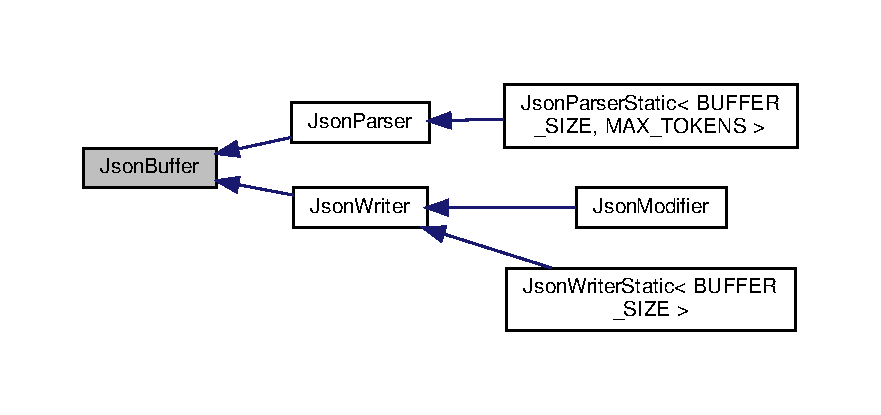
\includegraphics[width=350pt]{class_json_buffer__inherit__graph}
\end{center}
\end{figure}
\subsection*{Public Member Functions}
\begin{DoxyCompactItemize}
\item 
\hyperlink{class_json_buffer_a7198fe2dc430c6ebbc2374698c86f932}{Json\+Buffer} ()
\begin{DoxyCompactList}\small\item\em Construct a \hyperlink{class_json_buffer}{Json\+Buffer} object with no external buffer specified. \end{DoxyCompactList}\item 
virtual \hyperlink{class_json_buffer_a634ecf551d2d738b7a80b513e2c5a468}{$\sim$\+Json\+Buffer} ()
\begin{DoxyCompactList}\small\item\em Destructor. Destroying the object does not delete any underlying buffer! \end{DoxyCompactList}\item 
\hyperlink{class_json_buffer_a645819ad48ee172c01a482bef9c1f765}{Json\+Buffer} (char $\ast$\hyperlink{class_json_buffer_aaee27fe51d12d68bd6031df3bc78b6b5}{buffer}, size\+\_\+t \hyperlink{class_json_buffer_af06130f43f71623ea6afe049c846e52b}{buffer\+Len})
\begin{DoxyCompactList}\small\item\em Construct a \hyperlink{class_json_buffer}{Json\+Buffer} with an external buffer of a given size. \end{DoxyCompactList}\item 
void \hyperlink{class_json_buffer_a6721ab2b50d9b0bfc64d51c84c295230}{set\+Buffer} (char $\ast$\hyperlink{class_json_buffer_aaee27fe51d12d68bd6031df3bc78b6b5}{buffer}, size\+\_\+t \hyperlink{class_json_buffer_af06130f43f71623ea6afe049c846e52b}{buffer\+Len})
\begin{DoxyCompactList}\small\item\em Sets the buffers to the specified buffer and length. \end{DoxyCompactList}\item 
bool \hyperlink{class_json_buffer_a1eb9d0cae3ef9a9ac56b8580bc70fe2e}{allocate} (size\+\_\+t len)
\begin{DoxyCompactList}\small\item\em Allocate the buffer using malloc/realloc. \end{DoxyCompactList}\item 
bool \hyperlink{class_json_buffer_a61bf30ac6e1bd460f1e809d02a7d5ba4}{add\+String} (const char $\ast$data)
\begin{DoxyCompactList}\small\item\em Add a c-\/string to the end of the buffer. \end{DoxyCompactList}\item 
bool \hyperlink{class_json_buffer_a760cb5be42ed2d2ca9306b1109e76af3}{add\+Data} (const char $\ast$data, size\+\_\+t data\+Len)
\begin{DoxyCompactList}\small\item\em Add a string to the end of the buffer. \end{DoxyCompactList}\item 
char $\ast$ \hyperlink{class_json_buffer_af8ca5014e0275487273f94c6b9223acf}{get\+Buffer} () const
\begin{DoxyCompactList}\small\item\em Gets a pointer to the internal buffer. \end{DoxyCompactList}\item 
size\+\_\+t \hyperlink{class_json_buffer_adedc049fc02ef5bad2b3f8e7a1ba17b6}{get\+Offset} () const
\begin{DoxyCompactList}\small\item\em Gets the current offset for writing. \end{DoxyCompactList}\item 
void \hyperlink{class_json_buffer_a0043413c56e23d83f3b4dbe508a35315}{set\+Offset} (size\+\_\+t \hyperlink{class_json_buffer_aeb1ab3291108f351834f2e8c6784538c}{offset})
\begin{DoxyCompactList}\small\item\em swets the current offset for writing \end{DoxyCompactList}\item 
size\+\_\+t \hyperlink{class_json_buffer_a486352be5658e94b9b9bd13563801e68}{get\+Buffer\+Len} () const
\begin{DoxyCompactList}\small\item\em Gets the current length of the buffer. \end{DoxyCompactList}\item 
void \hyperlink{class_json_buffer_a70969847d857815a9ded6450378e0e53}{clear} ()
\begin{DoxyCompactList}\small\item\em Clears the current buffer for writing. \end{DoxyCompactList}\item 
void \hyperlink{class_json_buffer_a9f649ceeed76bb798c0bf9792b56d743}{null\+Terminate} ()
\begin{DoxyCompactList}\small\item\em Null terminates the buffer. \end{DoxyCompactList}\end{DoxyCompactItemize}
\subsection*{Protected Attributes}
\begin{DoxyCompactItemize}
\item 
char $\ast$ \hyperlink{class_json_buffer_aaee27fe51d12d68bd6031df3bc78b6b5}{buffer}
\begin{DoxyCompactList}\small\item\em The buffer to to read from or write to. This is not null-\/terminated. \end{DoxyCompactList}\item 
size\+\_\+t \hyperlink{class_json_buffer_af06130f43f71623ea6afe049c846e52b}{buffer\+Len}
\begin{DoxyCompactList}\small\item\em The length of the buffer in bytes,. \end{DoxyCompactList}\item 
size\+\_\+t \hyperlink{class_json_buffer_aeb1ab3291108f351834f2e8c6784538c}{offset}
\begin{DoxyCompactList}\small\item\em The read or write offset. \end{DoxyCompactList}\item 
bool \hyperlink{class_json_buffer_a729845e25c624d1dcb1da9712afbcdf7}{static\+Buffers}
\begin{DoxyCompactList}\small\item\em True if the buffers were passed in and should not freed or reallocated. \end{DoxyCompactList}\end{DoxyCompactItemize}


\subsection{Detailed Description}
Base class for managing a static or dynamic buffer, used by both \hyperlink{class_json_parser}{Json\+Parser} and \hyperlink{class_json_writer}{Json\+Writer}. 

Definition at line 146 of file Json\+Parser\+Generator\+R\+K.\+h.



\subsection{Constructor \& Destructor Documentation}
\mbox{\Hypertarget{class_json_buffer_a7198fe2dc430c6ebbc2374698c86f932}\label{class_json_buffer_a7198fe2dc430c6ebbc2374698c86f932}} 
\index{Json\+Buffer@{Json\+Buffer}!Json\+Buffer@{Json\+Buffer}}
\index{Json\+Buffer@{Json\+Buffer}!Json\+Buffer@{Json\+Buffer}}
\subsubsection{\texorpdfstring{Json\+Buffer()}{JsonBuffer()}\hspace{0.1cm}{\footnotesize\ttfamily [1/2]}}
{\footnotesize\ttfamily Json\+Buffer\+::\+Json\+Buffer (\begin{DoxyParamCaption}{ }\end{DoxyParamCaption})}



Construct a \hyperlink{class_json_buffer}{Json\+Buffer} object with no external buffer specified. 



Definition at line 6 of file Json\+Parser\+Generator\+R\+K.\+cpp.



References buffer, buffer\+Len, offset, and static\+Buffers.



Referenced by Json\+Parser\+::\+Json\+Parser(), and Json\+Writer\+::\+Json\+Writer().

\mbox{\Hypertarget{class_json_buffer_a634ecf551d2d738b7a80b513e2c5a468}\label{class_json_buffer_a634ecf551d2d738b7a80b513e2c5a468}} 
\index{Json\+Buffer@{Json\+Buffer}!````~Json\+Buffer@{$\sim$\+Json\+Buffer}}
\index{````~Json\+Buffer@{$\sim$\+Json\+Buffer}!Json\+Buffer@{Json\+Buffer}}
\subsubsection{\texorpdfstring{$\sim$\+Json\+Buffer()}{~JsonBuffer()}}
{\footnotesize\ttfamily Json\+Buffer\+::$\sim$\+Json\+Buffer (\begin{DoxyParamCaption}{ }\end{DoxyParamCaption})\hspace{0.3cm}{\ttfamily [virtual]}}



Destructor. Destroying the object does not delete any underlying buffer! 



Definition at line 9 of file Json\+Parser\+Generator\+R\+K.\+cpp.



References buffer, and static\+Buffers.

\mbox{\Hypertarget{class_json_buffer_a645819ad48ee172c01a482bef9c1f765}\label{class_json_buffer_a645819ad48ee172c01a482bef9c1f765}} 
\index{Json\+Buffer@{Json\+Buffer}!Json\+Buffer@{Json\+Buffer}}
\index{Json\+Buffer@{Json\+Buffer}!Json\+Buffer@{Json\+Buffer}}
\subsubsection{\texorpdfstring{Json\+Buffer()}{JsonBuffer()}\hspace{0.1cm}{\footnotesize\ttfamily [2/2]}}
{\footnotesize\ttfamily Json\+Buffer\+::\+Json\+Buffer (\begin{DoxyParamCaption}\item[{char $\ast$}]{buffer,  }\item[{size\+\_\+t}]{buffer\+Len }\end{DoxyParamCaption})}



Construct a \hyperlink{class_json_buffer}{Json\+Buffer} with an external buffer of a given size. 


\begin{DoxyParams}{Parameters}
{\em buffer} & Pointer to the buffer\\
\hline
{\em buffer\+Len} & The length of the buffer\\
\hline
\end{DoxyParams}
This buffer will not be deleted when the object is destructed. 

Definition at line 15 of file Json\+Parser\+Generator\+R\+K.\+cpp.



References buffer, buffer\+Len, offset, and static\+Buffers.



Referenced by Json\+Parser\+::\+Json\+Parser(), and Json\+Writer\+::\+Json\+Writer().



\subsection{Member Function Documentation}
\mbox{\Hypertarget{class_json_buffer_a760cb5be42ed2d2ca9306b1109e76af3}\label{class_json_buffer_a760cb5be42ed2d2ca9306b1109e76af3}} 
\index{Json\+Buffer@{Json\+Buffer}!add\+Data@{add\+Data}}
\index{add\+Data@{add\+Data}!Json\+Buffer@{Json\+Buffer}}
\subsubsection{\texorpdfstring{add\+Data()}{addData()}}
{\footnotesize\ttfamily bool Json\+Buffer\+::add\+Data (\begin{DoxyParamCaption}\item[{const char $\ast$}]{data,  }\item[{size\+\_\+t}]{data\+Len }\end{DoxyParamCaption})}



Add a string to the end of the buffer. 


\begin{DoxyParams}{Parameters}
{\em data} & Pointer to the string bytes. Does not need to be null-\/terminated\\
\hline
{\em data\+Len} & Length of the data in bytes. For U\+T\+F-\/8, this is the number of bytes, not characters! \\
\hline
\end{DoxyParams}


Definition at line 48 of file Json\+Parser\+Generator\+R\+K.\+cpp.



References allocate(), buffer, buffer\+Len, and offset.



Referenced by add\+String(), and main().

\mbox{\Hypertarget{class_json_buffer_a61bf30ac6e1bd460f1e809d02a7d5ba4}\label{class_json_buffer_a61bf30ac6e1bd460f1e809d02a7d5ba4}} 
\index{Json\+Buffer@{Json\+Buffer}!add\+String@{add\+String}}
\index{add\+String@{add\+String}!Json\+Buffer@{Json\+Buffer}}
\subsubsection{\texorpdfstring{add\+String()}{addString()}}
{\footnotesize\ttfamily bool Json\+Buffer\+::add\+String (\begin{DoxyParamCaption}\item[{const char $\ast$}]{data }\end{DoxyParamCaption})\hspace{0.3cm}{\ttfamily [inline]}}



Add a c-\/string to the end of the buffer. 


\begin{DoxyParams}{Parameters}
{\em data} & Pointer to a c-\/string (null terminated). \\
\hline
\end{DoxyParams}


Definition at line 197 of file Json\+Parser\+Generator\+R\+K.\+h.



References add\+Data().



Referenced by main(), run\+Test(), and subscription\+Handler().

\mbox{\Hypertarget{class_json_buffer_a1eb9d0cae3ef9a9ac56b8580bc70fe2e}\label{class_json_buffer_a1eb9d0cae3ef9a9ac56b8580bc70fe2e}} 
\index{Json\+Buffer@{Json\+Buffer}!allocate@{allocate}}
\index{allocate@{allocate}!Json\+Buffer@{Json\+Buffer}}
\subsubsection{\texorpdfstring{allocate()}{allocate()}}
{\footnotesize\ttfamily bool Json\+Buffer\+::allocate (\begin{DoxyParamCaption}\item[{size\+\_\+t}]{len }\end{DoxyParamCaption})}



Allocate the buffer using malloc/realloc. 


\begin{DoxyParams}{Parameters}
{\em len} & The length of the buffer in bytes\\
\hline
\end{DoxyParams}
\begin{DoxyReturn}{Returns}
true if the allocation/reallocation was successful or false if there was not enough free memory.
\end{DoxyReturn}
There\textquotesingle{}s also a version that takes a pointer and length to use a static buffer instead of a dynamically allocated one. 

Definition at line 25 of file Json\+Parser\+Generator\+R\+K.\+cpp.



References buffer, buffer\+Len, and static\+Buffers.



Referenced by add\+Data(), and main().

\mbox{\Hypertarget{class_json_buffer_a70969847d857815a9ded6450378e0e53}\label{class_json_buffer_a70969847d857815a9ded6450378e0e53}} 
\index{Json\+Buffer@{Json\+Buffer}!clear@{clear}}
\index{clear@{clear}!Json\+Buffer@{Json\+Buffer}}
\subsubsection{\texorpdfstring{clear()}{clear()}}
{\footnotesize\ttfamily void Json\+Buffer\+::clear (\begin{DoxyParamCaption}{ }\end{DoxyParamCaption})}



Clears the current buffer for writing. 

This only sets the offset to 0, it does not clear the bytes. 

Definition at line 62 of file Json\+Parser\+Generator\+R\+K.\+cpp.



References offset.



Referenced by get\+Measure\+\_\+callback(), run\+Test(), and subscription\+Handler().

\mbox{\Hypertarget{class_json_buffer_af8ca5014e0275487273f94c6b9223acf}\label{class_json_buffer_af8ca5014e0275487273f94c6b9223acf}} 
\index{Json\+Buffer@{Json\+Buffer}!get\+Buffer@{get\+Buffer}}
\index{get\+Buffer@{get\+Buffer}!Json\+Buffer@{Json\+Buffer}}
\subsubsection{\texorpdfstring{get\+Buffer()}{getBuffer()}}
{\footnotesize\ttfamily char$\ast$ Json\+Buffer\+::get\+Buffer (\begin{DoxyParamCaption}{ }\end{DoxyParamCaption}) const\hspace{0.3cm}{\ttfamily [inline]}}



Gets a pointer to the internal buffer. 

Note\+: The internal buffer is not null-\/terminated! 

Definition at line 213 of file Json\+Parser\+Generator\+R\+K.\+h.



References buffer.



Referenced by \+\_\+assert\+Json\+Parser\+Buffer(), \+\_\+assert\+Json\+Writer\+Buffer(), Json\+Modifier\+::find\+Left\+Comma(), Json\+Modifier\+::find\+Right\+Comma(), Json\+Modifier\+::finish(), print\+Json\+Inner(), print\+Token(), Json\+Modifier\+::remove\+Array\+Index(), Json\+Modifier\+::remove\+Key\+Value(), run\+Test(), Json\+Modifier\+::start\+Append(), and Json\+Modifier\+::start\+Modify().

\mbox{\Hypertarget{class_json_buffer_a486352be5658e94b9b9bd13563801e68}\label{class_json_buffer_a486352be5658e94b9b9bd13563801e68}} 
\index{Json\+Buffer@{Json\+Buffer}!get\+Buffer\+Len@{get\+Buffer\+Len}}
\index{get\+Buffer\+Len@{get\+Buffer\+Len}!Json\+Buffer@{Json\+Buffer}}
\subsubsection{\texorpdfstring{get\+Buffer\+Len()}{getBufferLen()}}
{\footnotesize\ttfamily size\+\_\+t Json\+Buffer\+::get\+Buffer\+Len (\begin{DoxyParamCaption}{ }\end{DoxyParamCaption}) const\hspace{0.3cm}{\ttfamily [inline]}}



Gets the current length of the buffer. 

The buffer length is either the buffer\+Len passed to the constructor that takes a buffer and buffer\+Len or the length allocated using allocate(len). 

Definition at line 231 of file Json\+Parser\+Generator\+R\+K.\+h.



References buffer\+Len.



Referenced by Json\+Modifier\+::start\+Append(), and Json\+Modifier\+::start\+Modify().

\mbox{\Hypertarget{class_json_buffer_adedc049fc02ef5bad2b3f8e7a1ba17b6}\label{class_json_buffer_adedc049fc02ef5bad2b3f8e7a1ba17b6}} 
\index{Json\+Buffer@{Json\+Buffer}!get\+Offset@{get\+Offset}}
\index{get\+Offset@{get\+Offset}!Json\+Buffer@{Json\+Buffer}}
\subsubsection{\texorpdfstring{get\+Offset()}{getOffset()}}
{\footnotesize\ttfamily size\+\_\+t Json\+Buffer\+::get\+Offset (\begin{DoxyParamCaption}{ }\end{DoxyParamCaption}) const\hspace{0.3cm}{\ttfamily [inline]}}



Gets the current offset for writing. 



Definition at line 218 of file Json\+Parser\+Generator\+R\+K.\+h.



References offset.



Referenced by \+\_\+assert\+Json\+Parser\+Buffer(), \+\_\+assert\+Json\+Writer\+Buffer(), Json\+Modifier\+::find\+Right\+Comma(), Json\+Modifier\+::finish(), Json\+Modifier\+::remove\+Array\+Index(), Json\+Modifier\+::remove\+Key\+Value(), Json\+Modifier\+::start\+Append(), and Json\+Modifier\+::start\+Modify().

\mbox{\Hypertarget{class_json_buffer_a9f649ceeed76bb798c0bf9792b56d743}\label{class_json_buffer_a9f649ceeed76bb798c0bf9792b56d743}} 
\index{Json\+Buffer@{Json\+Buffer}!null\+Terminate@{null\+Terminate}}
\index{null\+Terminate@{null\+Terminate}!Json\+Buffer@{Json\+Buffer}}
\subsubsection{\texorpdfstring{null\+Terminate()}{nullTerminate()}}
{\footnotesize\ttfamily void Json\+Buffer\+::null\+Terminate (\begin{DoxyParamCaption}{ }\end{DoxyParamCaption})}



Null terminates the buffer. 



Definition at line 66 of file Json\+Parser\+Generator\+R\+K.\+cpp.



References buffer, buffer\+Len, and offset.

\mbox{\Hypertarget{class_json_buffer_a6721ab2b50d9b0bfc64d51c84c295230}\label{class_json_buffer_a6721ab2b50d9b0bfc64d51c84c295230}} 
\index{Json\+Buffer@{Json\+Buffer}!set\+Buffer@{set\+Buffer}}
\index{set\+Buffer@{set\+Buffer}!Json\+Buffer@{Json\+Buffer}}
\subsubsection{\texorpdfstring{set\+Buffer()}{setBuffer()}}
{\footnotesize\ttfamily void Json\+Buffer\+::set\+Buffer (\begin{DoxyParamCaption}\item[{char $\ast$}]{buffer,  }\item[{size\+\_\+t}]{buffer\+Len }\end{DoxyParamCaption})}



Sets the buffers to the specified buffer and length. 


\begin{DoxyParams}{Parameters}
{\em buffer} & Pointer to the buffer\\
\hline
{\em buffer\+Len} & The length of the buffer\\
\hline
\end{DoxyParams}
This buffer will not be deleted when the object is destructed. 

Definition at line 19 of file Json\+Parser\+Generator\+R\+K.\+cpp.



References buffer, buffer\+Len, and static\+Buffers.



Referenced by Json\+Modifier\+::start\+Append(), and Json\+Modifier\+::start\+Modify().

\mbox{\Hypertarget{class_json_buffer_a0043413c56e23d83f3b4dbe508a35315}\label{class_json_buffer_a0043413c56e23d83f3b4dbe508a35315}} 
\index{Json\+Buffer@{Json\+Buffer}!set\+Offset@{set\+Offset}}
\index{set\+Offset@{set\+Offset}!Json\+Buffer@{Json\+Buffer}}
\subsubsection{\texorpdfstring{set\+Offset()}{setOffset()}}
{\footnotesize\ttfamily void Json\+Buffer\+::set\+Offset (\begin{DoxyParamCaption}\item[{size\+\_\+t}]{offset }\end{DoxyParamCaption})\hspace{0.3cm}{\ttfamily [inline]}}



swets the current offset for writing 



Definition at line 223 of file Json\+Parser\+Generator\+R\+K.\+h.



References offset.



Referenced by Json\+Modifier\+::finish(), Json\+Modifier\+::remove\+Array\+Index(), and Json\+Modifier\+::remove\+Key\+Value().



\subsection{Member Data Documentation}
\mbox{\Hypertarget{class_json_buffer_aaee27fe51d12d68bd6031df3bc78b6b5}\label{class_json_buffer_aaee27fe51d12d68bd6031df3bc78b6b5}} 
\index{Json\+Buffer@{Json\+Buffer}!buffer@{buffer}}
\index{buffer@{buffer}!Json\+Buffer@{Json\+Buffer}}
\subsubsection{\texorpdfstring{buffer}{buffer}}
{\footnotesize\ttfamily char$\ast$ Json\+Buffer\+::buffer\hspace{0.3cm}{\ttfamily [protected]}}



The buffer to to read from or write to. This is not null-\/terminated. 



Definition at line 246 of file Json\+Parser\+Generator\+R\+K.\+h.



Referenced by add\+Data(), allocate(), Json\+Parser\+::allocate\+Tokens(), Json\+Parser\+::copy\+Token\+Value(), Json\+Writer\+::finish\+Object\+Or\+Array(), get\+Buffer(), Json\+Parser\+::get\+Token\+Json\+String(), Json\+Parser\+::get\+Token\+Value(), Json\+Writer\+::insert\+Char(), Json\+Writer\+::insertvsprintf(), Json\+Buffer(), null\+Terminate(), Json\+Parser\+::parse(), set\+Buffer(), and $\sim$\+Json\+Buffer().

\mbox{\Hypertarget{class_json_buffer_af06130f43f71623ea6afe049c846e52b}\label{class_json_buffer_af06130f43f71623ea6afe049c846e52b}} 
\index{Json\+Buffer@{Json\+Buffer}!buffer\+Len@{buffer\+Len}}
\index{buffer\+Len@{buffer\+Len}!Json\+Buffer@{Json\+Buffer}}
\subsubsection{\texorpdfstring{buffer\+Len}{bufferLen}}
{\footnotesize\ttfamily size\+\_\+t Json\+Buffer\+::buffer\+Len\hspace{0.3cm}{\ttfamily [protected]}}



The length of the buffer in bytes,. 



Definition at line 247 of file Json\+Parser\+Generator\+R\+K.\+h.



Referenced by add\+Data(), allocate(), Json\+Writer\+::finish\+Object\+Or\+Array(), get\+Buffer\+Len(), Json\+Writer\+::insert\+Char(), Json\+Writer\+::insert\+String(), Json\+Writer\+::insertvsprintf(), Json\+Buffer(), null\+Terminate(), and set\+Buffer().

\mbox{\Hypertarget{class_json_buffer_aeb1ab3291108f351834f2e8c6784538c}\label{class_json_buffer_aeb1ab3291108f351834f2e8c6784538c}} 
\index{Json\+Buffer@{Json\+Buffer}!offset@{offset}}
\index{offset@{offset}!Json\+Buffer@{Json\+Buffer}}
\subsubsection{\texorpdfstring{offset}{offset}}
{\footnotesize\ttfamily size\+\_\+t Json\+Buffer\+::offset\hspace{0.3cm}{\ttfamily [protected]}}



The read or write offset. 



Definition at line 248 of file Json\+Parser\+Generator\+R\+K.\+h.



Referenced by add\+Data(), clear(), Json\+Writer\+::finish\+Object\+Or\+Array(), get\+Offset(), Json\+Writer\+::init(), Json\+Writer\+::insert\+Char(), Json\+Writer\+::insert\+String(), Json\+Writer\+::insertvsprintf(), Json\+Buffer(), null\+Terminate(), Json\+Parser\+::parse(), and set\+Offset().

\mbox{\Hypertarget{class_json_buffer_a729845e25c624d1dcb1da9712afbcdf7}\label{class_json_buffer_a729845e25c624d1dcb1da9712afbcdf7}} 
\index{Json\+Buffer@{Json\+Buffer}!static\+Buffers@{static\+Buffers}}
\index{static\+Buffers@{static\+Buffers}!Json\+Buffer@{Json\+Buffer}}
\subsubsection{\texorpdfstring{static\+Buffers}{staticBuffers}}
{\footnotesize\ttfamily bool Json\+Buffer\+::static\+Buffers\hspace{0.3cm}{\ttfamily [protected]}}



True if the buffers were passed in and should not freed or reallocated. 



Definition at line 249 of file Json\+Parser\+Generator\+R\+K.\+h.



Referenced by allocate(), Json\+Parser\+::allocate\+Tokens(), Json\+Buffer(), Json\+Parser\+::parse(), set\+Buffer(), $\sim$\+Json\+Buffer(), and Json\+Parser\+::$\sim$\+Json\+Parser().



The documentation for this class was generated from the following files\+:\begin{DoxyCompactItemize}
\item 
lib/\+Json\+Parser\+Generator\+R\+K/src/\hyperlink{_json_parser_generator_r_k_8h}{Json\+Parser\+Generator\+R\+K.\+h}\item 
lib/\+Json\+Parser\+Generator\+R\+K/src/\hyperlink{_json_parser_generator_r_k_8cpp}{Json\+Parser\+Generator\+R\+K.\+cpp}\end{DoxyCompactItemize}

\hypertarget{class_json_modifier}{}\section{Json\+Modifier Class Reference}
\label{class_json_modifier}\index{Json\+Modifier@{Json\+Modifier}}


Class for modifying a J\+S\+ON object in place, without needing to make a copy of it.  




{\ttfamily \#include $<$Json\+Parser\+Generator\+R\+K.\+h$>$}



Inheritance diagram for Json\+Modifier\+:
\nopagebreak
\begin{figure}[H]
\begin{center}
\leavevmode
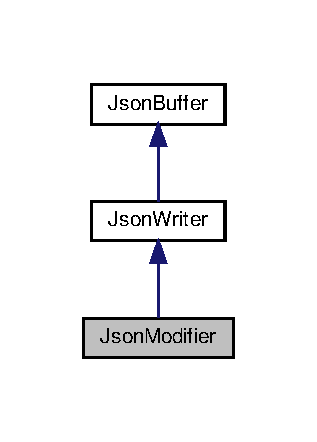
\includegraphics[width=152pt]{class_json_modifier__inherit__graph}
\end{center}
\end{figure}


Collaboration diagram for Json\+Modifier\+:
\nopagebreak
\begin{figure}[H]
\begin{center}
\leavevmode
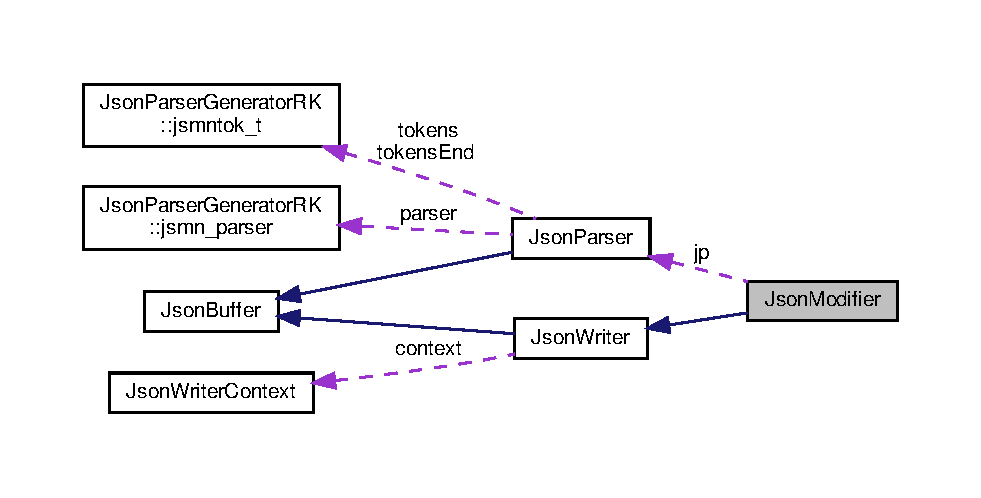
\includegraphics[width=350pt]{class_json_modifier__coll__graph}
\end{center}
\end{figure}
\subsection*{Public Member Functions}
\begin{DoxyCompactItemize}
\item 
\hyperlink{class_json_modifier_ac3d52284d9348720d59273bbbe228edf}{Json\+Modifier} (\hyperlink{class_json_parser}{Json\+Parser} \&\hyperlink{class_json_modifier_ab78d43036cea562e37640ae12e20b706}{jp})
\item 
virtual \hyperlink{class_json_modifier_a68e9b6a5b88ad4316fd1cb443cc0b11e}{$\sim$\+Json\+Modifier} ()
\item 
{\footnotesize template$<$class T $>$ }\\void \hyperlink{class_json_modifier_acca6028c0ec31489950f43e86c574229}{insert\+Or\+Update\+Key\+Value} (const \hyperlink{struct_json_parser_generator_r_k_1_1jsmntok__t}{Json\+Parser\+Generator\+R\+K\+::jsmntok\+\_\+t} $\ast$container, const char $\ast$key, T value)
\begin{DoxyCompactList}\small\item\em Inserts or updates a key/value pair into an object. \end{DoxyCompactList}\item 
{\footnotesize template$<$class T $>$ }\\void \hyperlink{class_json_modifier_ac492f5945ef4e4bc003fea5af5b9c504}{append\+Array\+Value} (const \hyperlink{struct_json_parser_generator_r_k_1_1jsmntok__t}{Json\+Parser\+Generator\+R\+K\+::jsmntok\+\_\+t} $\ast$array\+Token, T value)
\begin{DoxyCompactList}\small\item\em Appends a value to an array. \end{DoxyCompactList}\item 
bool \hyperlink{class_json_modifier_aadf76d2cef6b1a6ffe7868031cfb0e11}{remove\+Key\+Value} (const \hyperlink{struct_json_parser_generator_r_k_1_1jsmntok__t}{Json\+Parser\+Generator\+R\+K\+::jsmntok\+\_\+t} $\ast$container, const char $\ast$key)
\begin{DoxyCompactList}\small\item\em Removes a key and value from an object. \end{DoxyCompactList}\item 
bool \hyperlink{class_json_modifier_aba45c4fe467fa70b837f190986cf190b}{remove\+Array\+Index} (const \hyperlink{struct_json_parser_generator_r_k_1_1jsmntok__t}{Json\+Parser\+Generator\+R\+K\+::jsmntok\+\_\+t} $\ast$container, size\+\_\+t index)
\begin{DoxyCompactList}\small\item\em Removes an entry from an array. \end{DoxyCompactList}\item 
bool \hyperlink{class_json_modifier_aa53d66feb3cd13165f3a2eac012a123b}{start\+Modify} (const \hyperlink{struct_json_parser_generator_r_k_1_1jsmntok__t}{Json\+Parser\+Generator\+R\+K\+::jsmntok\+\_\+t} $\ast$token)
\begin{DoxyCompactList}\small\item\em Low level function to modify a token in place. \end{DoxyCompactList}\item 
bool \hyperlink{class_json_modifier_ab5bf356377a71120588413a4be998607}{start\+Append} (const \hyperlink{struct_json_parser_generator_r_k_1_1jsmntok__t}{Json\+Parser\+Generator\+R\+K\+::jsmntok\+\_\+t} $\ast$array\+Or\+Object\+Token)
\begin{DoxyCompactList}\small\item\em Low level function to append to an object or array. \end{DoxyCompactList}\item 
void \hyperlink{class_json_modifier_ae531232fa98f72eea8ea6ba07c065497}{finish} ()
\begin{DoxyCompactList}\small\item\em Finish modifying the object. \end{DoxyCompactList}\item 
\hyperlink{struct_json_parser_generator_r_k_1_1jsmntok__t}{Json\+Parser\+Generator\+R\+K\+::jsmntok\+\_\+t} \hyperlink{class_json_modifier_a5e685480ff2e978480cdc215b340e3a7}{token\+With\+Quotes} (const \hyperlink{struct_json_parser_generator_r_k_1_1jsmntok__t}{Json\+Parser\+Generator\+R\+K\+::jsmntok\+\_\+t} $\ast$tok) const
\begin{DoxyCompactList}\small\item\em Return a copy of tok, but moving so start and end include the double quotes for strings. \end{DoxyCompactList}\item 
int \hyperlink{class_json_modifier_a5b67ce1041b0e40e467639de1eeeca1e}{find\+Left\+Comma} (const \hyperlink{struct_json_parser_generator_r_k_1_1jsmntok__t}{Json\+Parser\+Generator\+R\+K\+::jsmntok\+\_\+t} $\ast$tok) const
\begin{DoxyCompactList}\small\item\em Find the offset of the comma to the left of the token, or -\/1 if there isn\textquotesingle{}t one. \end{DoxyCompactList}\item 
int \hyperlink{class_json_modifier_a24fac4c2257f932aff41792214de35ca}{find\+Right\+Comma} (const \hyperlink{struct_json_parser_generator_r_k_1_1jsmntok__t}{Json\+Parser\+Generator\+R\+K\+::jsmntok\+\_\+t} $\ast$tok) const
\begin{DoxyCompactList}\small\item\em Find the offset of the comma to the left of the token, or -\/1 if there isn\textquotesingle{}t one. \end{DoxyCompactList}\end{DoxyCompactItemize}
\subsection*{Protected Attributes}
\begin{DoxyCompactItemize}
\item 
\hyperlink{class_json_parser}{Json\+Parser} \& \hyperlink{class_json_modifier_ab78d43036cea562e37640ae12e20b706}{jp}
\begin{DoxyCompactList}\small\item\em The \hyperlink{class_json_parser}{Json\+Parser} object passed to the constructor. \end{DoxyCompactList}\item 
int \hyperlink{class_json_modifier_abd83b67763dc4ce55562bbdd5cea1e20}{start} = -\/1
\begin{DoxyCompactList}\small\item\em Start offset in the buffer. Set to -\/1 when \hyperlink{class_json_modifier_aa53d66feb3cd13165f3a2eac012a123b}{start\+Modify()} or \hyperlink{class_json_modifier_ab5bf356377a71120588413a4be998607}{start\+Append()} is not in progress. \end{DoxyCompactList}\item 
int \hyperlink{class_json_modifier_aec8c0683c15ad68dc1cb8180321bf902}{orig\+After} = 0
\begin{DoxyCompactList}\small\item\em Number of bytes after the insertion position, saved at save\+Loc when start is in progress. \end{DoxyCompactList}\item 
int \hyperlink{class_json_modifier_a7ea53418d660ce7cdec0964cca76015b}{save\+Loc} = 0
\begin{DoxyCompactList}\small\item\em Location where data is temporarily saved until \hyperlink{class_json_modifier_ae531232fa98f72eea8ea6ba07c065497}{finish()} is called. \end{DoxyCompactList}\end{DoxyCompactItemize}
\subsection*{Additional Inherited Members}


\subsection{Detailed Description}
Class for modifying a J\+S\+ON object in place, without needing to make a copy of it. 

Make sure the underlying \hyperlink{class_json_parser}{Json\+Parser} is big enough to hold the modified object. If you use Json\+Parser\+Static$<$$>$ make sure you have enough bytes and tokens.

The most commonly used method is \hyperlink{class_json_modifier_acca6028c0ec31489950f43e86c574229}{insert\+Or\+Update\+Key\+Value()}. This inserts or updates a key in an array. Another is \hyperlink{class_json_modifier_ac492f5945ef4e4bc003fea5af5b9c504}{append\+Array\+Value()} which appends a value to an array. Both methods are templated so you can use them with any valid type supported by \hyperlink{class_json_writer_ac58734c238ba7be066838591b0cc7743}{insert\+Value()} in \hyperlink{class_json_writer}{Json\+Writer}\+: bool, int, float, double, const char $\ast$.

This class is a subclass of \hyperlink{class_json_writer}{Json\+Writer}, so you can also use the low-\/level functions and \hyperlink{class_json_writer}{Json\+Writer} methods to do unusual object manipulations.

You can also use \hyperlink{class_json_modifier_aadf76d2cef6b1a6ffe7868031cfb0e11}{remove\+Key\+Value()} and \hyperlink{class_json_modifier_aba45c4fe467fa70b837f190986cf190b}{remove\+Array\+Index()} to remove keys or array entries. 

Definition at line 1323 of file Json\+Parser\+Generator\+R\+K.\+h.



\subsection{Constructor \& Destructor Documentation}
\mbox{\Hypertarget{class_json_modifier_ac3d52284d9348720d59273bbbe228edf}\label{class_json_modifier_ac3d52284d9348720d59273bbbe228edf}} 
\index{Json\+Modifier@{Json\+Modifier}!Json\+Modifier@{Json\+Modifier}}
\index{Json\+Modifier@{Json\+Modifier}!Json\+Modifier@{Json\+Modifier}}
\subsubsection{\texorpdfstring{Json\+Modifier()}{JsonModifier()}}
{\footnotesize\ttfamily Json\+Modifier\+::\+Json\+Modifier (\begin{DoxyParamCaption}\item[{\hyperlink{class_json_parser}{Json\+Parser} \&}]{jp }\end{DoxyParamCaption})}



Definition at line 881 of file Json\+Parser\+Generator\+R\+K.\+cpp.



References jp.

\mbox{\Hypertarget{class_json_modifier_a68e9b6a5b88ad4316fd1cb443cc0b11e}\label{class_json_modifier_a68e9b6a5b88ad4316fd1cb443cc0b11e}} 
\index{Json\+Modifier@{Json\+Modifier}!````~Json\+Modifier@{$\sim$\+Json\+Modifier}}
\index{````~Json\+Modifier@{$\sim$\+Json\+Modifier}!Json\+Modifier@{Json\+Modifier}}
\subsubsection{\texorpdfstring{$\sim$\+Json\+Modifier()}{~JsonModifier()}}
{\footnotesize\ttfamily Json\+Modifier\+::$\sim$\+Json\+Modifier (\begin{DoxyParamCaption}{ }\end{DoxyParamCaption})\hspace{0.3cm}{\ttfamily [virtual]}}



Definition at line 885 of file Json\+Parser\+Generator\+R\+K.\+cpp.



\subsection{Member Function Documentation}
\mbox{\Hypertarget{class_json_modifier_ac492f5945ef4e4bc003fea5af5b9c504}\label{class_json_modifier_ac492f5945ef4e4bc003fea5af5b9c504}} 
\index{Json\+Modifier@{Json\+Modifier}!append\+Array\+Value@{append\+Array\+Value}}
\index{append\+Array\+Value@{append\+Array\+Value}!Json\+Modifier@{Json\+Modifier}}
\subsubsection{\texorpdfstring{append\+Array\+Value()}{appendArrayValue()}}
{\footnotesize\ttfamily template$<$class T $>$ \\
void Json\+Modifier\+::append\+Array\+Value (\begin{DoxyParamCaption}\item[{const \hyperlink{struct_json_parser_generator_r_k_1_1jsmntok__t}{Json\+Parser\+Generator\+R\+K\+::jsmntok\+\_\+t} $\ast$}]{array\+Token,  }\item[{T}]{value }\end{DoxyParamCaption})\hspace{0.3cm}{\ttfamily [inline]}}



Appends a value to an array. 

Uses templates so you can pass any type object that\textquotesingle{}s supported by \hyperlink{class_json_writer_ac58734c238ba7be066838591b0cc7743}{insert\+Value()} overloads, for example\+: bool, int, float, double, const char $\ast$.

To modify the outermost array, use jp.\+get\+Outer\+Array() for the array\+Token. You can also modify arrays in an object using get\+Value\+Token\+By\+Key().

Note\+: This method call jp.\+parse() so any jsmntok\+\_\+t may be changed by this method. If you\textquotesingle{}ve fetched one, such as by using get\+Value\+Token\+By\+Key() be sure to fetch it again to be safe. 

Definition at line 1363 of file Json\+Parser\+Generator\+R\+K.\+h.



References finish(), and start\+Append().

\mbox{\Hypertarget{class_json_modifier_a5b67ce1041b0e40e467639de1eeeca1e}\label{class_json_modifier_a5b67ce1041b0e40e467639de1eeeca1e}} 
\index{Json\+Modifier@{Json\+Modifier}!find\+Left\+Comma@{find\+Left\+Comma}}
\index{find\+Left\+Comma@{find\+Left\+Comma}!Json\+Modifier@{Json\+Modifier}}
\subsubsection{\texorpdfstring{find\+Left\+Comma()}{findLeftComma()}}
{\footnotesize\ttfamily int Json\+Modifier\+::find\+Left\+Comma (\begin{DoxyParamCaption}\item[{const \hyperlink{struct_json_parser_generator_r_k_1_1jsmntok__t}{Json\+Parser\+Generator\+R\+K\+::jsmntok\+\_\+t} $\ast$}]{tok }\end{DoxyParamCaption}) const}



Find the offset of the comma to the left of the token, or -\/1 if there isn\textquotesingle{}t one. 

Used internally, you probably won\textquotesingle{}t need to use this. 

Definition at line 1058 of file Json\+Parser\+Generator\+R\+K.\+cpp.



References Json\+Buffer\+::get\+Buffer(), jp, Json\+Parser\+Generator\+R\+K\+::jsmntok\+\_\+t\+::start, and token\+With\+Quotes().



Referenced by remove\+Array\+Index(), and remove\+Key\+Value().

\mbox{\Hypertarget{class_json_modifier_a24fac4c2257f932aff41792214de35ca}\label{class_json_modifier_a24fac4c2257f932aff41792214de35ca}} 
\index{Json\+Modifier@{Json\+Modifier}!find\+Right\+Comma@{find\+Right\+Comma}}
\index{find\+Right\+Comma@{find\+Right\+Comma}!Json\+Modifier@{Json\+Modifier}}
\subsubsection{\texorpdfstring{find\+Right\+Comma()}{findRightComma()}}
{\footnotesize\ttfamily int Json\+Modifier\+::find\+Right\+Comma (\begin{DoxyParamCaption}\item[{const \hyperlink{struct_json_parser_generator_r_k_1_1jsmntok__t}{Json\+Parser\+Generator\+R\+K\+::jsmntok\+\_\+t} $\ast$}]{tok }\end{DoxyParamCaption}) const}



Find the offset of the comma to the left of the token, or -\/1 if there isn\textquotesingle{}t one. 

Used internally, you probably won\textquotesingle{}t need to use this. 

Definition at line 1077 of file Json\+Parser\+Generator\+R\+K.\+cpp.



References Json\+Parser\+Generator\+R\+K\+::jsmntok\+\_\+t\+::end, Json\+Buffer\+::get\+Buffer(), Json\+Buffer\+::get\+Offset(), jp, and token\+With\+Quotes().



Referenced by remove\+Array\+Index(), and remove\+Key\+Value().

\mbox{\Hypertarget{class_json_modifier_ae531232fa98f72eea8ea6ba07c065497}\label{class_json_modifier_ae531232fa98f72eea8ea6ba07c065497}} 
\index{Json\+Modifier@{Json\+Modifier}!finish@{finish}}
\index{finish@{finish}!Json\+Modifier@{Json\+Modifier}}
\subsubsection{\texorpdfstring{finish()}{finish()}}
{\footnotesize\ttfamily void Json\+Modifier\+::finish (\begin{DoxyParamCaption}{ }\end{DoxyParamCaption})}



Finish modifying the object. 

Finish must be called after start\+Modify or start\+Append otherwise the object will be corrupted.

Note\+: This method call jp.\+parse() so any jsmntok\+\_\+t may be changed by this method. If you\textquotesingle{}ve fetched one, such as by using get\+Value\+Token\+By\+Key() be sure to fetch it again to be safe.

The high level function like insert\+Or\+Update\+Key\+Value, append\+Array\+Value, remove\+Key\+Value, and remove\+Array\+Index internally call finish so you should not call it again with those methods. 

Definition at line 1033 of file Json\+Parser\+Generator\+R\+K.\+cpp.



References Json\+Buffer\+::get\+Offset(), jp, orig\+After, Json\+Parser\+::parse(), Json\+Buffer\+::set\+Offset(), and start.



Referenced by append\+Array\+Value(), insert\+Or\+Update\+Key\+Value(), and main().

\mbox{\Hypertarget{class_json_modifier_acca6028c0ec31489950f43e86c574229}\label{class_json_modifier_acca6028c0ec31489950f43e86c574229}} 
\index{Json\+Modifier@{Json\+Modifier}!insert\+Or\+Update\+Key\+Value@{insert\+Or\+Update\+Key\+Value}}
\index{insert\+Or\+Update\+Key\+Value@{insert\+Or\+Update\+Key\+Value}!Json\+Modifier@{Json\+Modifier}}
\subsubsection{\texorpdfstring{insert\+Or\+Update\+Key\+Value()}{insertOrUpdateKeyValue()}}
{\footnotesize\ttfamily template$<$class T $>$ \\
void Json\+Modifier\+::insert\+Or\+Update\+Key\+Value (\begin{DoxyParamCaption}\item[{const \hyperlink{struct_json_parser_generator_r_k_1_1jsmntok__t}{Json\+Parser\+Generator\+R\+K\+::jsmntok\+\_\+t} $\ast$}]{container,  }\item[{const char $\ast$}]{key,  }\item[{T}]{value }\end{DoxyParamCaption})\hspace{0.3cm}{\ttfamily [inline]}}



Inserts or updates a key/value pair into an object. 

Uses templates so you can pass any type object that\textquotesingle{}s supported by \hyperlink{class_json_writer_ac58734c238ba7be066838591b0cc7743}{insert\+Value()} overloads, for example\+: bool, int, float, double, const char $\ast$.

To modify the outermost object, use jp.\+get\+Outer\+Object() for the container.

Note\+: This method call jp.\+parse() so any jsmntok\+\_\+t may be changed by this method. If you\textquotesingle{}ve fetched one, such as by using get\+Value\+Token\+By\+Key() be sure to fetch it again to be safe. 

Definition at line 1340 of file Json\+Parser\+Generator\+R\+K.\+h.



References finish(), remove\+Key\+Value(), and start\+Append().

\mbox{\Hypertarget{class_json_modifier_aba45c4fe467fa70b837f190986cf190b}\label{class_json_modifier_aba45c4fe467fa70b837f190986cf190b}} 
\index{Json\+Modifier@{Json\+Modifier}!remove\+Array\+Index@{remove\+Array\+Index}}
\index{remove\+Array\+Index@{remove\+Array\+Index}!Json\+Modifier@{Json\+Modifier}}
\subsubsection{\texorpdfstring{remove\+Array\+Index()}{removeArrayIndex()}}
{\footnotesize\ttfamily bool Json\+Modifier\+::remove\+Array\+Index (\begin{DoxyParamCaption}\item[{const \hyperlink{struct_json_parser_generator_r_k_1_1jsmntok__t}{Json\+Parser\+Generator\+R\+K\+::jsmntok\+\_\+t} $\ast$}]{container,  }\item[{size\+\_\+t}]{index }\end{DoxyParamCaption})}



Removes an entry from an array. 

Note\+: This method call jp.\+parse() so any jsmntok\+\_\+t may be changed by this method. If you\textquotesingle{}ve fetched one, such as by using get\+Value\+Token\+By\+Key() be sure to fetch it again to be safe. 

Definition at line 944 of file Json\+Parser\+Generator\+R\+K.\+cpp.



References Json\+Parser\+Generator\+R\+K\+::jsmntok\+\_\+t\+::end, find\+Left\+Comma(), find\+Right\+Comma(), Json\+Buffer\+::get\+Offset(), Json\+Parser\+::get\+Token\+By\+Index(), jp, orig\+After, Json\+Parser\+::parse(), Json\+Buffer\+::set\+Offset(), Json\+Parser\+Generator\+R\+K\+::jsmntok\+\_\+t\+::start, and token\+With\+Quotes().



Referenced by main().

\mbox{\Hypertarget{class_json_modifier_aadf76d2cef6b1a6ffe7868031cfb0e11}\label{class_json_modifier_aadf76d2cef6b1a6ffe7868031cfb0e11}} 
\index{Json\+Modifier@{Json\+Modifier}!remove\+Key\+Value@{remove\+Key\+Value}}
\index{remove\+Key\+Value@{remove\+Key\+Value}!Json\+Modifier@{Json\+Modifier}}
\subsubsection{\texorpdfstring{remove\+Key\+Value()}{removeKeyValue()}}
{\footnotesize\ttfamily bool Json\+Modifier\+::remove\+Key\+Value (\begin{DoxyParamCaption}\item[{const \hyperlink{struct_json_parser_generator_r_k_1_1jsmntok__t}{Json\+Parser\+Generator\+R\+K\+::jsmntok\+\_\+t} $\ast$}]{container,  }\item[{const char $\ast$}]{key }\end{DoxyParamCaption})}



Removes a key and value from an object. 

Note\+: This method call jp.\+parse() so any jsmntok\+\_\+t may be changed by this method. If you\textquotesingle{}ve fetched one, such as by using get\+Value\+Token\+By\+Key() be sure to fetch it again to be safe. 

Definition at line 890 of file Json\+Parser\+Generator\+R\+K.\+cpp.



References Json\+Parser\+Generator\+R\+K\+::jsmntok\+\_\+t\+::end, find\+Left\+Comma(), find\+Right\+Comma(), Json\+Buffer\+::get\+Offset(), Json\+Parser\+::get\+Value\+Token\+By\+Key(), jp, orig\+After, Json\+Parser\+::parse(), Json\+Buffer\+::set\+Offset(), Json\+Parser\+Generator\+R\+K\+::jsmntok\+\_\+t\+::start, and token\+With\+Quotes().



Referenced by insert\+Or\+Update\+Key\+Value().

\mbox{\Hypertarget{class_json_modifier_ab5bf356377a71120588413a4be998607}\label{class_json_modifier_ab5bf356377a71120588413a4be998607}} 
\index{Json\+Modifier@{Json\+Modifier}!start\+Append@{start\+Append}}
\index{start\+Append@{start\+Append}!Json\+Modifier@{Json\+Modifier}}
\subsubsection{\texorpdfstring{start\+Append()}{startAppend()}}
{\footnotesize\ttfamily bool Json\+Modifier\+::start\+Append (\begin{DoxyParamCaption}\item[{const \hyperlink{struct_json_parser_generator_r_k_1_1jsmntok__t}{Json\+Parser\+Generator\+R\+K\+::jsmntok\+\_\+t} $\ast$}]{array\+Or\+Object\+Token }\end{DoxyParamCaption})}



Low level function to append to an object or array. 


\begin{DoxyParams}{Parameters}
{\em array\+Or\+Object\+Token} & the jsmntok\+\_\+t to append to. This must be an object or array token.\\
\hline
\end{DoxyParams}
You must call \hyperlink{class_json_modifier_ae531232fa98f72eea8ea6ba07c065497}{finish()} after modification is done to restore the object to a valid state. 

Definition at line 1009 of file Json\+Parser\+Generator\+R\+K.\+cpp.



References Json\+Parser\+Generator\+R\+K\+::jsmntok\+\_\+t\+::end, Json\+Buffer\+::get\+Buffer(), Json\+Buffer\+::get\+Buffer\+Len(), Json\+Buffer\+::get\+Offset(), Json\+Writer\+::init(), jp, orig\+After, save\+Loc, Json\+Buffer\+::set\+Buffer(), Json\+Writer\+::set\+Is\+First(), Json\+Parser\+Generator\+R\+K\+::jsmntok\+\_\+t\+::size, and start.



Referenced by append\+Array\+Value(), insert\+Or\+Update\+Key\+Value(), and main().

\mbox{\Hypertarget{class_json_modifier_aa53d66feb3cd13165f3a2eac012a123b}\label{class_json_modifier_aa53d66feb3cd13165f3a2eac012a123b}} 
\index{Json\+Modifier@{Json\+Modifier}!start\+Modify@{start\+Modify}}
\index{start\+Modify@{start\+Modify}!Json\+Modifier@{Json\+Modifier}}
\subsubsection{\texorpdfstring{start\+Modify()}{startModify()}}
{\footnotesize\ttfamily bool Json\+Modifier\+::start\+Modify (\begin{DoxyParamCaption}\item[{const \hyperlink{struct_json_parser_generator_r_k_1_1jsmntok__t}{Json\+Parser\+Generator\+R\+K\+::jsmntok\+\_\+t} $\ast$}]{token }\end{DoxyParamCaption})}



Low level function to modify a token in place. 


\begin{DoxyParams}{Parameters}
{\em token} & the jsmntok\+\_\+t to modify\\
\hline
\end{DoxyParams}
You must call \hyperlink{class_json_modifier_ae531232fa98f72eea8ea6ba07c065497}{finish()} after modification is done to restore the object to a valid state!

Note\+: \hyperlink{class_json_modifier_acca6028c0ec31489950f43e86c574229}{insert\+Or\+Update\+Key\+Value()} does not use this. Instead it removes then appends the new value. The reason is that start\+Modify does not work if you change the type of the data to or from a string. This is tricky to deal with correctly, so it\textquotesingle{}s easier to just remove and add the item again. 

Definition at line 988 of file Json\+Parser\+Generator\+R\+K.\+cpp.



References Json\+Parser\+Generator\+R\+K\+::jsmntok\+\_\+t\+::end, Json\+Buffer\+::get\+Buffer(), Json\+Buffer\+::get\+Buffer\+Len(), Json\+Buffer\+::get\+Offset(), Json\+Writer\+::init(), jp, orig\+After, save\+Loc, Json\+Buffer\+::set\+Buffer(), Json\+Parser\+Generator\+R\+K\+::jsmntok\+\_\+t\+::start, and start.



Referenced by main().

\mbox{\Hypertarget{class_json_modifier_a5e685480ff2e978480cdc215b340e3a7}\label{class_json_modifier_a5e685480ff2e978480cdc215b340e3a7}} 
\index{Json\+Modifier@{Json\+Modifier}!token\+With\+Quotes@{token\+With\+Quotes}}
\index{token\+With\+Quotes@{token\+With\+Quotes}!Json\+Modifier@{Json\+Modifier}}
\subsubsection{\texorpdfstring{token\+With\+Quotes()}{tokenWithQuotes()}}
{\footnotesize\ttfamily \hyperlink{struct_json_parser_generator_r_k_1_1jsmntok__t}{Json\+Parser\+Generator\+R\+K\+::jsmntok\+\_\+t} Json\+Modifier\+::token\+With\+Quotes (\begin{DoxyParamCaption}\item[{const \hyperlink{struct_json_parser_generator_r_k_1_1jsmntok__t}{Json\+Parser\+Generator\+R\+K\+::jsmntok\+\_\+t} $\ast$}]{tok }\end{DoxyParamCaption}) const}



Return a copy of tok, but moving so start and end include the double quotes for strings. 

Used internally, you probably won\textquotesingle{}t need to use this. 

Definition at line 1048 of file Json\+Parser\+Generator\+R\+K.\+cpp.



References Json\+Parser\+Generator\+R\+K\+::jsmntok\+\_\+t\+::end, Json\+Parser\+Generator\+R\+K\+::\+J\+S\+M\+N\+\_\+\+S\+T\+R\+I\+NG, Json\+Parser\+Generator\+R\+K\+::jsmntok\+\_\+t\+::start, and Json\+Parser\+Generator\+R\+K\+::jsmntok\+\_\+t\+::type.



Referenced by find\+Left\+Comma(), find\+Right\+Comma(), remove\+Array\+Index(), and remove\+Key\+Value().



\subsection{Member Data Documentation}
\mbox{\Hypertarget{class_json_modifier_ab78d43036cea562e37640ae12e20b706}\label{class_json_modifier_ab78d43036cea562e37640ae12e20b706}} 
\index{Json\+Modifier@{Json\+Modifier}!jp@{jp}}
\index{jp@{jp}!Json\+Modifier@{Json\+Modifier}}
\subsubsection{\texorpdfstring{jp}{jp}}
{\footnotesize\ttfamily \hyperlink{class_json_parser}{Json\+Parser}\& Json\+Modifier\+::jp\hspace{0.3cm}{\ttfamily [protected]}}



The \hyperlink{class_json_parser}{Json\+Parser} object passed to the constructor. 



Definition at line 1447 of file Json\+Parser\+Generator\+R\+K.\+h.



Referenced by find\+Left\+Comma(), find\+Right\+Comma(), finish(), Json\+Modifier(), remove\+Array\+Index(), remove\+Key\+Value(), start\+Append(), and start\+Modify().

\mbox{\Hypertarget{class_json_modifier_aec8c0683c15ad68dc1cb8180321bf902}\label{class_json_modifier_aec8c0683c15ad68dc1cb8180321bf902}} 
\index{Json\+Modifier@{Json\+Modifier}!orig\+After@{orig\+After}}
\index{orig\+After@{orig\+After}!Json\+Modifier@{Json\+Modifier}}
\subsubsection{\texorpdfstring{orig\+After}{origAfter}}
{\footnotesize\ttfamily int Json\+Modifier\+::orig\+After = 0\hspace{0.3cm}{\ttfamily [protected]}}



Number of bytes after the insertion position, saved at save\+Loc when start is in progress. 



Definition at line 1449 of file Json\+Parser\+Generator\+R\+K.\+h.



Referenced by finish(), remove\+Array\+Index(), remove\+Key\+Value(), start\+Append(), and start\+Modify().

\mbox{\Hypertarget{class_json_modifier_a7ea53418d660ce7cdec0964cca76015b}\label{class_json_modifier_a7ea53418d660ce7cdec0964cca76015b}} 
\index{Json\+Modifier@{Json\+Modifier}!save\+Loc@{save\+Loc}}
\index{save\+Loc@{save\+Loc}!Json\+Modifier@{Json\+Modifier}}
\subsubsection{\texorpdfstring{save\+Loc}{saveLoc}}
{\footnotesize\ttfamily int Json\+Modifier\+::save\+Loc = 0\hspace{0.3cm}{\ttfamily [protected]}}



Location where data is temporarily saved until \hyperlink{class_json_modifier_ae531232fa98f72eea8ea6ba07c065497}{finish()} is called. 



Definition at line 1450 of file Json\+Parser\+Generator\+R\+K.\+h.



Referenced by start\+Append(), and start\+Modify().

\mbox{\Hypertarget{class_json_modifier_abd83b67763dc4ce55562bbdd5cea1e20}\label{class_json_modifier_abd83b67763dc4ce55562bbdd5cea1e20}} 
\index{Json\+Modifier@{Json\+Modifier}!start@{start}}
\index{start@{start}!Json\+Modifier@{Json\+Modifier}}
\subsubsection{\texorpdfstring{start}{start}}
{\footnotesize\ttfamily int Json\+Modifier\+::start = -\/1\hspace{0.3cm}{\ttfamily [protected]}}



Start offset in the buffer. Set to -\/1 when \hyperlink{class_json_modifier_aa53d66feb3cd13165f3a2eac012a123b}{start\+Modify()} or \hyperlink{class_json_modifier_ab5bf356377a71120588413a4be998607}{start\+Append()} is not in progress. 



Definition at line 1448 of file Json\+Parser\+Generator\+R\+K.\+h.



Referenced by finish(), start\+Append(), and start\+Modify().



The documentation for this class was generated from the following files\+:\begin{DoxyCompactItemize}
\item 
lib/\+Json\+Parser\+Generator\+R\+K/src/\hyperlink{_json_parser_generator_r_k_8h}{Json\+Parser\+Generator\+R\+K.\+h}\item 
lib/\+Json\+Parser\+Generator\+R\+K/src/\hyperlink{_json_parser_generator_r_k_8cpp}{Json\+Parser\+Generator\+R\+K.\+cpp}\end{DoxyCompactItemize}

\hypertarget{class_json_parser}{}\section{Json\+Parser Class Reference}
\label{class_json_parser}\index{Json\+Parser@{Json\+Parser}}


A\+PI to the \hyperlink{class_json_parser}{Json\+Parser}.  




{\ttfamily \#include $<$Json\+Parser\+Generator\+R\+K.\+h$>$}



Inheritance diagram for Json\+Parser\+:
\nopagebreak
\begin{figure}[H]
\begin{center}
\leavevmode
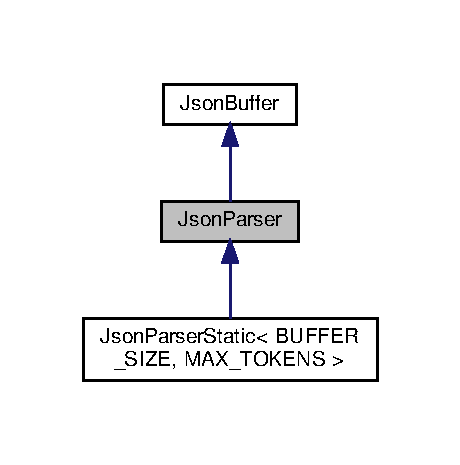
\includegraphics[width=221pt]{class_json_parser__inherit__graph}
\end{center}
\end{figure}


Collaboration diagram for Json\+Parser\+:
\nopagebreak
\begin{figure}[H]
\begin{center}
\leavevmode
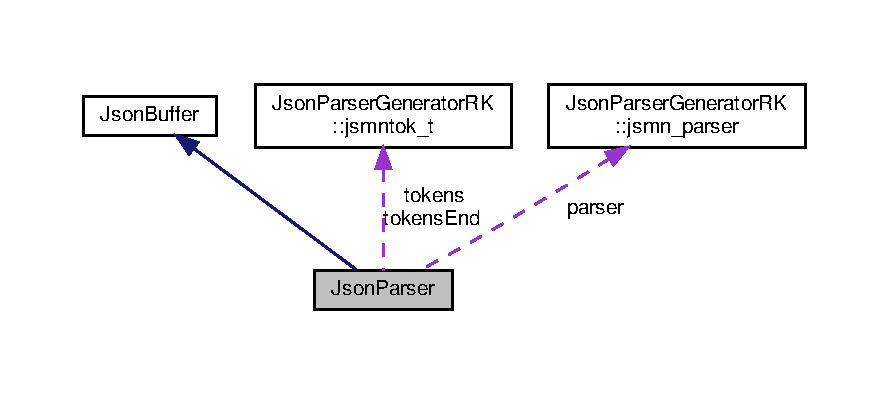
\includegraphics[width=350pt]{class_json_parser__coll__graph}
\end{center}
\end{figure}
\subsection*{Public Member Functions}
\begin{DoxyCompactItemize}
\item 
\hyperlink{class_json_parser_af21abdfb0ceac731e44d897a0285f5d4}{Json\+Parser} ()
\begin{DoxyCompactList}\small\item\em Construct a parser object. \end{DoxyCompactList}\item 
virtual \hyperlink{class_json_parser_a7c0393b54c37f9ff30b6bb59f0ba92ce}{$\sim$\+Json\+Parser} ()
\begin{DoxyCompactList}\small\item\em Destroy a parser object. \end{DoxyCompactList}\item 
\hyperlink{class_json_parser_a394f8fa82e72240ce4ad6e6ca25700b6}{Json\+Parser} (char $\ast$\hyperlink{class_json_buffer_aaee27fe51d12d68bd6031df3bc78b6b5}{buffer}, size\+\_\+t \hyperlink{class_json_buffer_af06130f43f71623ea6afe049c846e52b}{buffer\+Len}, \hyperlink{struct_json_parser_generator_r_k_1_1jsmntok__t}{Json\+Parser\+Generator\+R\+K\+::jsmntok\+\_\+t} $\ast$\hyperlink{class_json_parser_af2a9bba1dc92b0c38d0cab6fdad76216}{tokens}, size\+\_\+t \hyperlink{class_json_parser_a0dfa97de05bac37c5be2e1ee9747b8a2}{max\+Tokens})
\begin{DoxyCompactList}\small\item\em Static buffers constructor. \end{DoxyCompactList}\item 
bool \hyperlink{class_json_parser_a1731e3265d6b2f89587638dcd6d7ff34}{allocate\+Tokens} (size\+\_\+t \hyperlink{class_json_parser_a0dfa97de05bac37c5be2e1ee9747b8a2}{max\+Tokens})
\begin{DoxyCompactList}\small\item\em Preallocates a specific number of tokens. \end{DoxyCompactList}\item 
bool \hyperlink{class_json_parser_ad528213e8600cbad4d85910b62fc033a}{parse} ()
\begin{DoxyCompactList}\small\item\em Parses the data you have added using \hyperlink{class_json_buffer_a760cb5be42ed2d2ca9306b1109e76af3}{add\+Data()} or \hyperlink{class_json_buffer_a61bf30ac6e1bd460f1e809d02a7d5ba4}{add\+String()}. \end{DoxyCompactList}\item 
\hyperlink{class_json_reference}{Json\+Reference} \hyperlink{class_json_parser_a27f639337cff7b364edb05c01f098786}{get\+Reference} () const
\begin{DoxyCompactList}\small\item\em Get a \hyperlink{class_json_reference}{Json\+Reference} object. This is used for fluent-\/style access to the data. \end{DoxyCompactList}\item 
const \hyperlink{struct_json_parser_generator_r_k_1_1jsmntok__t}{Json\+Parser\+Generator\+R\+K\+::jsmntok\+\_\+t} $\ast$ \hyperlink{class_json_parser_a4e694318a7c823d4cca3a5be49907df7}{get\+Outer\+Object} () const
\begin{DoxyCompactList}\small\item\em Gets the outer J\+S\+ON object token. \end{DoxyCompactList}\item 
const \hyperlink{struct_json_parser_generator_r_k_1_1jsmntok__t}{Json\+Parser\+Generator\+R\+K\+::jsmntok\+\_\+t} $\ast$ \hyperlink{class_json_parser_a91ffa7e1c4d2fbc2524533d65c31b605}{get\+Outer\+Array} () const
\begin{DoxyCompactList}\small\item\em Gets the outer J\+S\+ON array token. \end{DoxyCompactList}\item 
const \hyperlink{struct_json_parser_generator_r_k_1_1jsmntok__t}{Json\+Parser\+Generator\+R\+K\+::jsmntok\+\_\+t} $\ast$ \hyperlink{class_json_parser_a3c28b01c0e1fc3c7677e07e1739ea288}{get\+Outer\+Token} () const
\begin{DoxyCompactList}\small\item\em Gets the outer J\+S\+ON object or array token. \end{DoxyCompactList}\item 
size\+\_\+t \hyperlink{class_json_parser_aeb46af21c13fa2396e065543bd8db265}{get\+Array\+Size} (const \hyperlink{struct_json_parser_generator_r_k_1_1jsmntok__t}{Json\+Parser\+Generator\+R\+K\+::jsmntok\+\_\+t} $\ast$array\+Container) const
\begin{DoxyCompactList}\small\item\em Given a token for an J\+S\+ON array in array\+Container, gets the number of elements in the array. \end{DoxyCompactList}\item 
{\footnotesize template$<$class T $>$ }\\bool \hyperlink{class_json_parser_a13abcdcb2341f65ac358bb4d81007d06}{get\+Value\+By\+Key} (const \hyperlink{struct_json_parser_generator_r_k_1_1jsmntok__t}{Json\+Parser\+Generator\+R\+K\+::jsmntok\+\_\+t} $\ast$container, const char $\ast$name, T \&result) const
\begin{DoxyCompactList}\small\item\em Given an object token in container, gets the value with the specified key name. \end{DoxyCompactList}\item 
{\footnotesize template$<$class T $>$ }\\bool \hyperlink{class_json_parser_a38858994342cd2735b716b117bf8afdf}{get\+Outer\+Value\+By\+Key} (const char $\ast$name, T \&result) const
\begin{DoxyCompactList}\small\item\em Gets the value with the specified key name out of the outer object. \end{DoxyCompactList}\item 
{\footnotesize template$<$class T $>$ }\\bool \hyperlink{class_json_parser_a5759f53499dcb4418e07e9c5e1a42442}{get\+Key\+Value\+By\+Index} (const \hyperlink{struct_json_parser_generator_r_k_1_1jsmntok__t}{Json\+Parser\+Generator\+R\+K\+::jsmntok\+\_\+t} $\ast$container, size\+\_\+t index, \hyperlink{class_string}{String} \&key, T \&result) const
\begin{DoxyCompactList}\small\item\em Gets the key/value pair of an object by index. \end{DoxyCompactList}\item 
{\footnotesize template$<$class T $>$ }\\bool \hyperlink{class_json_parser_a4718893bc6350e129a9acbf6cb5a47ad}{get\+Outer\+Key\+Value\+By\+Index} (size\+\_\+t index, \hyperlink{class_string}{String} \&key, T \&result) const
\begin{DoxyCompactList}\small\item\em Gets the key/value pair of the outer object by index (0 = first, 1 = second, ...) \end{DoxyCompactList}\item 
{\footnotesize template$<$class T $>$ }\\bool \hyperlink{class_json_parser_a53bd8a6ebb0d9b246b876653e792368f}{get\+Value\+By\+Index} (const \hyperlink{struct_json_parser_generator_r_k_1_1jsmntok__t}{Json\+Parser\+Generator\+R\+K\+::jsmntok\+\_\+t} $\ast$array\+Container, size\+\_\+t index, T \&result) const
\begin{DoxyCompactList}\small\item\em Given an array token in array\+Container, gets the value with the specified index. \end{DoxyCompactList}\item 
{\footnotesize template$<$class T $>$ }\\bool \hyperlink{class_json_parser_af1f4a3a65b5cc9cd19b129c410aa78e0}{get\+Value\+By\+Col\+Row} (const \hyperlink{struct_json_parser_generator_r_k_1_1jsmntok__t}{Json\+Parser\+Generator\+R\+K\+::jsmntok\+\_\+t} $\ast$array\+Container, size\+\_\+t col, size\+\_\+t row, T \&result) const
\begin{DoxyCompactList}\small\item\em This method is used to extract data from a 2-\/dimensional J\+S\+ON array, an array of arrays of values. \end{DoxyCompactList}\item 
bool \hyperlink{class_json_parser_a39d613e94d0d6beafe908159f86bc067}{get\+Value\+Token\+By\+Key} (const \hyperlink{struct_json_parser_generator_r_k_1_1jsmntok__t}{Json\+Parser\+Generator\+R\+K\+::jsmntok\+\_\+t} $\ast$container, const char $\ast$key, const \hyperlink{struct_json_parser_generator_r_k_1_1jsmntok__t}{Json\+Parser\+Generator\+R\+K\+::jsmntok\+\_\+t} $\ast$\&value) const
\begin{DoxyCompactList}\small\item\em Given an object token in container, gets the token value with the specified key name. \end{DoxyCompactList}\item 
bool \hyperlink{class_json_parser_a680846b3e3e3e1d40c27bbb71e080048}{get\+Value\+Token\+By\+Index} (const \hyperlink{struct_json_parser_generator_r_k_1_1jsmntok__t}{Json\+Parser\+Generator\+R\+K\+::jsmntok\+\_\+t} $\ast$container, size\+\_\+t desired\+Index, const \hyperlink{struct_json_parser_generator_r_k_1_1jsmntok__t}{Json\+Parser\+Generator\+R\+K\+::jsmntok\+\_\+t} $\ast$\&value) const
\begin{DoxyCompactList}\small\item\em Given an array token in container, gets the token value with the specified index. \end{DoxyCompactList}\item 
bool \hyperlink{class_json_parser_a4fc494206dd45eba5959ffc2df444a21}{get\+Value\+Token\+By\+Col\+Row} (const \hyperlink{struct_json_parser_generator_r_k_1_1jsmntok__t}{Json\+Parser\+Generator\+R\+K\+::jsmntok\+\_\+t} $\ast$container, size\+\_\+t col, size\+\_\+t row, const \hyperlink{struct_json_parser_generator_r_k_1_1jsmntok__t}{Json\+Parser\+Generator\+R\+K\+::jsmntok\+\_\+t} $\ast$\&value) const
\begin{DoxyCompactList}\small\item\em This method is used to extract data from a 2-\/dimensional J\+S\+ON array, an array of arrays of values. \end{DoxyCompactList}\item 
const \hyperlink{struct_json_parser_generator_r_k_1_1jsmntok__t}{Json\+Parser\+Generator\+R\+K\+::jsmntok\+\_\+t} $\ast$ \hyperlink{class_json_parser_a588d9c4fcfe9179db67ca42f5ba5229d}{get\+Token\+By\+Index} (const \hyperlink{struct_json_parser_generator_r_k_1_1jsmntok__t}{Json\+Parser\+Generator\+R\+K\+::jsmntok\+\_\+t} $\ast$container, size\+\_\+t desired\+Index) const
\begin{DoxyCompactList}\small\item\em Given a containing object, finds the nth token in the object. Internal use only. \end{DoxyCompactList}\item 
bool \hyperlink{class_json_parser_a946929ab0c54eed7e7c8697e9304d553}{get\+Key\+Value\+Token\+By\+Index} (const \hyperlink{struct_json_parser_generator_r_k_1_1jsmntok__t}{Json\+Parser\+Generator\+R\+K\+::jsmntok\+\_\+t} $\ast$container, const \hyperlink{struct_json_parser_generator_r_k_1_1jsmntok__t}{Json\+Parser\+Generator\+R\+K\+::jsmntok\+\_\+t} $\ast$\&key, const \hyperlink{struct_json_parser_generator_r_k_1_1jsmntok__t}{Json\+Parser\+Generator\+R\+K\+::jsmntok\+\_\+t} $\ast$\&value, size\+\_\+t index) const
\begin{DoxyCompactList}\small\item\em Given a J\+S\+ON object in container, gets the key/value pair specified by index. Internal use only. \end{DoxyCompactList}\item 
bool \hyperlink{class_json_parser_a182ab93b3639f0a99f37f9101eb48361}{skip\+Object} (const \hyperlink{struct_json_parser_generator_r_k_1_1jsmntok__t}{Json\+Parser\+Generator\+R\+K\+::jsmntok\+\_\+t} $\ast$container, const \hyperlink{struct_json_parser_generator_r_k_1_1jsmntok__t}{Json\+Parser\+Generator\+R\+K\+::jsmntok\+\_\+t} $\ast$\&obj) const
\begin{DoxyCompactList}\small\item\em Used internally to skip over the token in obj. \end{DoxyCompactList}\item 
void \hyperlink{class_json_parser_ab7f8a2873dd3a2935cf0a22133a5378f}{copy\+Token\+Value} (const \hyperlink{struct_json_parser_generator_r_k_1_1jsmntok__t}{Json\+Parser\+Generator\+R\+K\+::jsmntok\+\_\+t} $\ast$token, char $\ast$dst, size\+\_\+t dst\+Len) const
\begin{DoxyCompactList}\small\item\em Copies the value of the token into a buffer, making it a null-\/terminated cstring. \end{DoxyCompactList}\item 
bool \hyperlink{class_json_parser_a5f9e5c2453307a99a54fcf26fbd68dd4}{get\+Token\+Value} (const \hyperlink{struct_json_parser_generator_r_k_1_1jsmntok__t}{Json\+Parser\+Generator\+R\+K\+::jsmntok\+\_\+t} $\ast$token, bool \&result) const
\begin{DoxyCompactList}\small\item\em Gets a bool (boolean) value. \end{DoxyCompactList}\item 
bool \hyperlink{class_json_parser_a875e5b4b01c9cd597e09b13e59fe6252}{get\+Token\+Value} (const \hyperlink{struct_json_parser_generator_r_k_1_1jsmntok__t}{Json\+Parser\+Generator\+R\+K\+::jsmntok\+\_\+t} $\ast$token, int \&result) const
\begin{DoxyCompactList}\small\item\em Gets an integer value. \end{DoxyCompactList}\item 
bool \hyperlink{class_json_parser_ad6289b63a2281dc516e4a81aa3660ac7}{get\+Token\+Value} (const \hyperlink{struct_json_parser_generator_r_k_1_1jsmntok__t}{Json\+Parser\+Generator\+R\+K\+::jsmntok\+\_\+t} $\ast$token, unsigned long \&result) const
\begin{DoxyCompactList}\small\item\em Gets an unsigned long value. \end{DoxyCompactList}\item 
bool \hyperlink{class_json_parser_a37a6ad66b9697ceb6b789b4c9abaa3ab}{get\+Token\+Value} (const \hyperlink{struct_json_parser_generator_r_k_1_1jsmntok__t}{Json\+Parser\+Generator\+R\+K\+::jsmntok\+\_\+t} $\ast$token, float \&result) const
\begin{DoxyCompactList}\small\item\em Gets a float (single precision floating point) value. \end{DoxyCompactList}\item 
bool \hyperlink{class_json_parser_af378b1400c3f091ae6ba67dc588ca863}{get\+Token\+Value} (const \hyperlink{struct_json_parser_generator_r_k_1_1jsmntok__t}{Json\+Parser\+Generator\+R\+K\+::jsmntok\+\_\+t} $\ast$token, double \&result) const
\begin{DoxyCompactList}\small\item\em Gets a double (double precision floating point) value. \end{DoxyCompactList}\item 
bool \hyperlink{class_json_parser_a44cff567586e80ba63d39324e5929672}{get\+Token\+Value} (const \hyperlink{struct_json_parser_generator_r_k_1_1jsmntok__t}{Json\+Parser\+Generator\+R\+K\+::jsmntok\+\_\+t} $\ast$token, \hyperlink{class_string}{String} \&result) const
\begin{DoxyCompactList}\small\item\em Gets a \hyperlink{class_string}{String} value into a Wiring \hyperlink{class_string}{String} object. \end{DoxyCompactList}\item 
bool \hyperlink{class_json_parser_aa5c0b33d4ddeae1e0d605e166a2a772c}{get\+Token\+Value} (const \hyperlink{struct_json_parser_generator_r_k_1_1jsmntok__t}{Json\+Parser\+Generator\+R\+K\+::jsmntok\+\_\+t} $\ast$token, char $\ast$str, size\+\_\+t \&str\+Len) const
\begin{DoxyCompactList}\small\item\em Gets a string as a c-\/string into the specified buffer. \end{DoxyCompactList}\item 
bool \hyperlink{class_json_parser_a6942f718b6b73d2ff1611f55aec8569c}{get\+Token\+Value} (const \hyperlink{struct_json_parser_generator_r_k_1_1jsmntok__t}{Json\+Parser\+Generator\+R\+K\+::jsmntok\+\_\+t} $\ast$token, \hyperlink{class_json_parser_string}{Json\+Parser\+String} \&str) const
\begin{DoxyCompactList}\small\item\em Gets a string as a \hyperlink{class_json_parser_string}{Json\+Parser\+String} object. \end{DoxyCompactList}\item 
bool \hyperlink{class_json_parser_a334ccfff663a5d3155a799049896d55c}{get\+Token\+Json\+String} (const \hyperlink{struct_json_parser_generator_r_k_1_1jsmntok__t}{Json\+Parser\+Generator\+R\+K\+::jsmntok\+\_\+t} $\ast$token, \hyperlink{class_string}{String} \&result) const
\begin{DoxyCompactList}\small\item\em Converts a token (object, array, string, or primitive) back into J\+S\+ON in a Wiring \hyperlink{class_string}{String}. \end{DoxyCompactList}\item 
bool \hyperlink{class_json_parser_af235693afede52de81794e3773e5cff4}{get\+Token\+Json\+String} (const \hyperlink{struct_json_parser_generator_r_k_1_1jsmntok__t}{Json\+Parser\+Generator\+R\+K\+::jsmntok\+\_\+t} $\ast$token, char $\ast$str, size\+\_\+t \&str\+Len) const
\begin{DoxyCompactList}\small\item\em Converts a token (object, array, string, or primitive) back into J\+S\+ON in a buffer. \end{DoxyCompactList}\item 
bool \hyperlink{class_json_parser_a4c6d9fc64d49d057dd2b7b3ea63a7d8c}{get\+Token\+Json\+String} (const \hyperlink{struct_json_parser_generator_r_k_1_1jsmntok__t}{Json\+Parser\+Generator\+R\+K\+::jsmntok\+\_\+t} $\ast$token, \hyperlink{class_json_parser_string}{Json\+Parser\+String} \&str) const
\begin{DoxyCompactList}\small\item\em Gets a token as a J\+S\+ON string. \end{DoxyCompactList}\item 
\hyperlink{struct_json_parser_generator_r_k_1_1jsmntok__t}{Json\+Parser\+Generator\+R\+K\+::jsmntok\+\_\+t} $\ast$ \hyperlink{class_json_parser_a1cdeae1e2cf1b45cde47ca8a8f9a84c9}{get\+Tokens} ()
\begin{DoxyCompactList}\small\item\em Used internally in the test suite for printing the token list. \end{DoxyCompactList}\item 
\hyperlink{struct_json_parser_generator_r_k_1_1jsmntok__t}{Json\+Parser\+Generator\+R\+K\+::jsmntok\+\_\+t} $\ast$ \hyperlink{class_json_parser_a8e0503af76c2bc9b8d2231dddb8b1cb3}{get\+Tokens\+End} ()
\begin{DoxyCompactList}\small\item\em Used internally in the test suite for printing the token list. \end{DoxyCompactList}\item 
size\+\_\+t \hyperlink{class_json_parser_a39e91342fbbb72d6fb304dd2f2e7f505}{get\+Max\+Tokens} () const
\begin{DoxyCompactList}\small\item\em Used internally in the test suite for printing the token list. \end{DoxyCompactList}\end{DoxyCompactItemize}
\subsection*{Static Public Member Functions}
\begin{DoxyCompactItemize}
\item 
static void \hyperlink{class_json_parser_a498dcdec7949c88dfc454d052e25ff69}{append\+Utf8} (uint16\+\_\+t unicode, \hyperlink{class_json_parser_string}{Json\+Parser\+String} \&str)
\begin{DoxyCompactList}\small\item\em Given a Unicode U\+T\+F-\/16 code point, converts it to U\+T\+F-\/8 and appends it to str. \end{DoxyCompactList}\end{DoxyCompactItemize}
\subsection*{Protected Attributes}
\begin{DoxyCompactItemize}
\item 
\hyperlink{struct_json_parser_generator_r_k_1_1jsmntok__t}{Json\+Parser\+Generator\+R\+K\+::jsmntok\+\_\+t} $\ast$ \hyperlink{class_json_parser_af2a9bba1dc92b0c38d0cab6fdad76216}{tokens}
\begin{DoxyCompactList}\small\item\em Array of tokens after parsing. \end{DoxyCompactList}\item 
\hyperlink{struct_json_parser_generator_r_k_1_1jsmntok__t}{Json\+Parser\+Generator\+R\+K\+::jsmntok\+\_\+t} $\ast$ \hyperlink{class_json_parser_a6b8c13ce885f8bc7470248d0dc56f157}{tokens\+End}
\begin{DoxyCompactList}\small\item\em Pointer into tokens, points after last used token. \end{DoxyCompactList}\item 
size\+\_\+t \hyperlink{class_json_parser_a0dfa97de05bac37c5be2e1ee9747b8a2}{max\+Tokens}
\begin{DoxyCompactList}\small\item\em Number of tokens that can be stored in tokens. \end{DoxyCompactList}\item 
\hyperlink{struct_json_parser_generator_r_k_1_1jsmn__parser}{Json\+Parser\+Generator\+R\+K\+::jsmn\+\_\+parser} \hyperlink{class_json_parser_ad8d3dc7a971bd6c8e578518ba6c874f9}{parser}
\begin{DoxyCompactList}\small\item\em The J\+S\+MN parser object. \end{DoxyCompactList}\end{DoxyCompactItemize}
\subsection*{Friends}
\begin{DoxyCompactItemize}
\item 
class \hyperlink{class_json_parser_a26df0cdb3650a4a46921ba1793ecfd03}{Json\+Modifier}
\end{DoxyCompactItemize}


\subsection{Detailed Description}
A\+PI to the \hyperlink{class_json_parser}{Json\+Parser}. 

This is a memory-\/efficient J\+S\+ON parser based on jsmn. It only keeps one copy of the data in raw format and an array of tokens. You make calls to read values out. 

Definition at line 262 of file Json\+Parser\+Generator\+R\+K.\+h.



\subsection{Constructor \& Destructor Documentation}
\mbox{\Hypertarget{class_json_parser_af21abdfb0ceac731e44d897a0285f5d4}\label{class_json_parser_af21abdfb0ceac731e44d897a0285f5d4}} 
\index{Json\+Parser@{Json\+Parser}!Json\+Parser@{Json\+Parser}}
\index{Json\+Parser@{Json\+Parser}!Json\+Parser@{Json\+Parser}}
\subsubsection{\texorpdfstring{Json\+Parser()}{JsonParser()}\hspace{0.1cm}{\footnotesize\ttfamily [1/2]}}
{\footnotesize\ttfamily Json\+Parser\+::\+Json\+Parser (\begin{DoxyParamCaption}{ }\end{DoxyParamCaption})}



Construct a parser object. 

This version dynamically allocates the buffer and token storage. If you want to minimize memory allocations you can pass in a static buffer and array of tokens to use instead. 

Definition at line 80 of file Json\+Parser\+Generator\+R\+K.\+cpp.



References Json\+Buffer\+::\+Json\+Buffer(), max\+Tokens, tokens, and tokens\+End.

\mbox{\Hypertarget{class_json_parser_a7c0393b54c37f9ff30b6bb59f0ba92ce}\label{class_json_parser_a7c0393b54c37f9ff30b6bb59f0ba92ce}} 
\index{Json\+Parser@{Json\+Parser}!````~Json\+Parser@{$\sim$\+Json\+Parser}}
\index{````~Json\+Parser@{$\sim$\+Json\+Parser}!Json\+Parser@{Json\+Parser}}
\subsubsection{\texorpdfstring{$\sim$\+Json\+Parser()}{~JsonParser()}}
{\footnotesize\ttfamily Json\+Parser\+::$\sim$\+Json\+Parser (\begin{DoxyParamCaption}{ }\end{DoxyParamCaption})\hspace{0.3cm}{\ttfamily [virtual]}}



Destroy a parser object. 

If the buffer was allocated dynamically it will be deleted. If you passed in a static buffer the static buffer is not deleted. 

Definition at line 89 of file Json\+Parser\+Generator\+R\+K.\+cpp.



References Json\+Buffer\+::static\+Buffers, and tokens.

\mbox{\Hypertarget{class_json_parser_a394f8fa82e72240ce4ad6e6ca25700b6}\label{class_json_parser_a394f8fa82e72240ce4ad6e6ca25700b6}} 
\index{Json\+Parser@{Json\+Parser}!Json\+Parser@{Json\+Parser}}
\index{Json\+Parser@{Json\+Parser}!Json\+Parser@{Json\+Parser}}
\subsubsection{\texorpdfstring{Json\+Parser()}{JsonParser()}\hspace{0.1cm}{\footnotesize\ttfamily [2/2]}}
{\footnotesize\ttfamily Json\+Parser\+::\+Json\+Parser (\begin{DoxyParamCaption}\item[{char $\ast$}]{buffer,  }\item[{size\+\_\+t}]{buffer\+Len,  }\item[{\hyperlink{struct_json_parser_generator_r_k_1_1jsmntok__t}{Json\+Parser\+Generator\+R\+K\+::jsmntok\+\_\+t} $\ast$}]{tokens,  }\item[{size\+\_\+t}]{max\+Tokens }\end{DoxyParamCaption})}



Static buffers constructor. 



Definition at line 83 of file Json\+Parser\+Generator\+R\+K.\+cpp.



References Json\+Buffer\+::\+Json\+Buffer(), max\+Tokens, and tokens.



\subsection{Member Function Documentation}
\mbox{\Hypertarget{class_json_parser_a1731e3265d6b2f89587638dcd6d7ff34}\label{class_json_parser_a1731e3265d6b2f89587638dcd6d7ff34}} 
\index{Json\+Parser@{Json\+Parser}!allocate\+Tokens@{allocate\+Tokens}}
\index{allocate\+Tokens@{allocate\+Tokens}!Json\+Parser@{Json\+Parser}}
\subsubsection{\texorpdfstring{allocate\+Tokens()}{allocateTokens()}}
{\footnotesize\ttfamily bool Json\+Parser\+::allocate\+Tokens (\begin{DoxyParamCaption}\item[{size\+\_\+t}]{max\+Tokens }\end{DoxyParamCaption})}



Preallocates a specific number of tokens. 

Optional\+: You should set this larger than the expected number of tokens for efficiency, but if you are not using the static allocator it will resize the token storage space if it\textquotesingle{}s too small. 

Definition at line 95 of file Json\+Parser\+Generator\+R\+K.\+cpp.



References max\+Tokens, Json\+Buffer\+::static\+Buffers, and tokens.

\mbox{\Hypertarget{class_json_parser_a498dcdec7949c88dfc454d052e25ff69}\label{class_json_parser_a498dcdec7949c88dfc454d052e25ff69}} 
\index{Json\+Parser@{Json\+Parser}!append\+Utf8@{append\+Utf8}}
\index{append\+Utf8@{append\+Utf8}!Json\+Parser@{Json\+Parser}}
\subsubsection{\texorpdfstring{append\+Utf8()}{appendUtf8()}}
{\footnotesize\ttfamily void Json\+Parser\+::append\+Utf8 (\begin{DoxyParamCaption}\item[{uint16\+\_\+t}]{unicode,  }\item[{\hyperlink{class_json_parser_string}{Json\+Parser\+String} \&}]{str }\end{DoxyParamCaption})\hspace{0.3cm}{\ttfamily [static]}}



Given a Unicode U\+T\+F-\/16 code point, converts it to U\+T\+F-\/8 and appends it to str. 



Definition at line 509 of file Json\+Parser\+Generator\+R\+K.\+cpp.



References Json\+Parser\+String\+::append().

\mbox{\Hypertarget{class_json_parser_ab7f8a2873dd3a2935cf0a22133a5378f}\label{class_json_parser_ab7f8a2873dd3a2935cf0a22133a5378f}} 
\index{Json\+Parser@{Json\+Parser}!copy\+Token\+Value@{copy\+Token\+Value}}
\index{copy\+Token\+Value@{copy\+Token\+Value}!Json\+Parser@{Json\+Parser}}
\subsubsection{\texorpdfstring{copy\+Token\+Value()}{copyTokenValue()}}
{\footnotesize\ttfamily void Json\+Parser\+::copy\+Token\+Value (\begin{DoxyParamCaption}\item[{const \hyperlink{struct_json_parser_generator_r_k_1_1jsmntok__t}{Json\+Parser\+Generator\+R\+K\+::jsmntok\+\_\+t} $\ast$}]{token,  }\item[{char $\ast$}]{dst,  }\item[{size\+\_\+t}]{dst\+Len }\end{DoxyParamCaption}) const}



Copies the value of the token into a buffer, making it a null-\/terminated cstring. 

If the string is longer than dst\+Len -\/ 1 bytes, it will be truncated and the result will still be a valid cstring.

This is used internally because the token data is not null-\/terminated, and doing things like sscanf or strtoul on it can read past the end of the buffer. This assures that only null-\/terminated data is passed to these functions. 

Definition at line 327 of file Json\+Parser\+Generator\+R\+K.\+cpp.



References Json\+Buffer\+::buffer, Json\+Parser\+Generator\+R\+K\+::jsmntok\+\_\+t\+::end, and Json\+Parser\+Generator\+R\+K\+::jsmntok\+\_\+t\+::start.



Referenced by get\+Token\+Value().

\mbox{\Hypertarget{class_json_parser_aeb46af21c13fa2396e065543bd8db265}\label{class_json_parser_aeb46af21c13fa2396e065543bd8db265}} 
\index{Json\+Parser@{Json\+Parser}!get\+Array\+Size@{get\+Array\+Size}}
\index{get\+Array\+Size@{get\+Array\+Size}!Json\+Parser@{Json\+Parser}}
\subsubsection{\texorpdfstring{get\+Array\+Size()}{getArraySize()}}
{\footnotesize\ttfamily size\+\_\+t Json\+Parser\+::get\+Array\+Size (\begin{DoxyParamCaption}\item[{const \hyperlink{struct_json_parser_generator_r_k_1_1jsmntok__t}{Json\+Parser\+Generator\+R\+K\+::jsmntok\+\_\+t} $\ast$}]{array\+Container }\end{DoxyParamCaption}) const}



Given a token for an J\+S\+ON array in array\+Container, gets the number of elements in the array. 

0 = no elements, 1 = one element, ...

The index values for \hyperlink{class_json_parser_a53bd8a6ebb0d9b246b876653e792368f}{get\+Value\+By\+Index()}, etc. are 0-\/based, so the last index you pass in is less than \hyperlink{class_json_parser_aeb46af21c13fa2396e065543bd8db265}{get\+Array\+Size()}. 

Definition at line 315 of file Json\+Parser\+Generator\+R\+K.\+cpp.



References Json\+Parser\+Generator\+R\+K\+::jsmntok\+\_\+t\+::end, skip\+Object(), and tokens\+End.



Referenced by Json\+Reference\+::size().

\mbox{\Hypertarget{class_json_parser_a5759f53499dcb4418e07e9c5e1a42442}\label{class_json_parser_a5759f53499dcb4418e07e9c5e1a42442}} 
\index{Json\+Parser@{Json\+Parser}!get\+Key\+Value\+By\+Index@{get\+Key\+Value\+By\+Index}}
\index{get\+Key\+Value\+By\+Index@{get\+Key\+Value\+By\+Index}!Json\+Parser@{Json\+Parser}}
\subsubsection{\texorpdfstring{get\+Key\+Value\+By\+Index()}{getKeyValueByIndex()}}
{\footnotesize\ttfamily template$<$class T $>$ \\
bool Json\+Parser\+::get\+Key\+Value\+By\+Index (\begin{DoxyParamCaption}\item[{const \hyperlink{struct_json_parser_generator_r_k_1_1jsmntok__t}{Json\+Parser\+Generator\+R\+K\+::jsmntok\+\_\+t} $\ast$}]{container,  }\item[{size\+\_\+t}]{index,  }\item[{\hyperlink{class_string}{String} \&}]{key,  }\item[{T \&}]{result }\end{DoxyParamCaption}) const\hspace{0.3cm}{\ttfamily [inline]}}



Gets the key/value pair of an object by index. 


\begin{DoxyParams}{Parameters}
{\em container} & The object to look in (see get\+Outer\+Key\+Value\+By\+Index if you want to the outermost object you parsed)\\
\hline
{\em index} & 0 = first, 1 = second, ...\\
\hline
{\em key} & Filled in with the name of the key\\
\hline
{\em result} & Filled in with the value. The value can be of type\+: bool, int, unsigned long, float, double, \hyperlink{class_string}{String}, or (char $\ast$, size\+\_\+t\&).\\
\hline
\end{DoxyParams}
\begin{DoxyReturn}{Returns}
true if the call succeeded or false if it failed.
\end{DoxyReturn}
Normally you get a value in an object by its key, but if you want to iterate all of the keys you can use this method. Call it until it returns false.

This should only be used for things like string, numbers, booleans, etc.. If you want to get a J\+S\+ON array or object within an object, use \hyperlink{class_json_parser_a39d613e94d0d6beafe908159f86bc067}{get\+Value\+Token\+By\+Key()} instead. 

Definition at line 425 of file Json\+Parser\+Generator\+R\+K.\+h.



References get\+Key\+Value\+Token\+By\+Index().

\mbox{\Hypertarget{class_json_parser_a946929ab0c54eed7e7c8697e9304d553}\label{class_json_parser_a946929ab0c54eed7e7c8697e9304d553}} 
\index{Json\+Parser@{Json\+Parser}!get\+Key\+Value\+Token\+By\+Index@{get\+Key\+Value\+Token\+By\+Index}}
\index{get\+Key\+Value\+Token\+By\+Index@{get\+Key\+Value\+Token\+By\+Index}!Json\+Parser@{Json\+Parser}}
\subsubsection{\texorpdfstring{get\+Key\+Value\+Token\+By\+Index()}{getKeyValueTokenByIndex()}}
{\footnotesize\ttfamily bool Json\+Parser\+::get\+Key\+Value\+Token\+By\+Index (\begin{DoxyParamCaption}\item[{const \hyperlink{struct_json_parser_generator_r_k_1_1jsmntok__t}{Json\+Parser\+Generator\+R\+K\+::jsmntok\+\_\+t} $\ast$}]{container,  }\item[{const \hyperlink{struct_json_parser_generator_r_k_1_1jsmntok__t}{Json\+Parser\+Generator\+R\+K\+::jsmntok\+\_\+t} $\ast$\&}]{key,  }\item[{const \hyperlink{struct_json_parser_generator_r_k_1_1jsmntok__t}{Json\+Parser\+Generator\+R\+K\+::jsmntok\+\_\+t} $\ast$\&}]{value,  }\item[{size\+\_\+t}]{index }\end{DoxyParamCaption}) const}



Given a J\+S\+ON object in container, gets the key/value pair specified by index. Internal use only. 


\begin{DoxyParams}{Parameters}
{\em container} & The array token to look in.\\
\hline
{\em key} & Filled in with the key token for nth key value pair.\\
\hline
{\em value} & Filled in with the value token for then nth key value pair.\\
\hline
{\em index} & The index to retrieve (0 = first, 1 = second, ...).\\
\hline
\end{DoxyParams}
This is a low-\/level function; you will typically use \hyperlink{class_json_parser_a53bd8a6ebb0d9b246b876653e792368f}{get\+Value\+By\+Index()} or \hyperlink{class_json_parser_a13abcdcb2341f65ac358bb4d81007d06}{get\+Value\+By\+Key()} instead. 

Definition at line 250 of file Json\+Parser\+Generator\+R\+K.\+cpp.



References Json\+Parser\+Generator\+R\+K\+::jsmntok\+\_\+t\+::end, skip\+Object(), and tokens\+End.



Referenced by get\+Key\+Value\+By\+Index(), get\+Value\+Token\+By\+Key(), main(), and print\+Json\+Inner().

\mbox{\Hypertarget{class_json_parser_a39e91342fbbb72d6fb304dd2f2e7f505}\label{class_json_parser_a39e91342fbbb72d6fb304dd2f2e7f505}} 
\index{Json\+Parser@{Json\+Parser}!get\+Max\+Tokens@{get\+Max\+Tokens}}
\index{get\+Max\+Tokens@{get\+Max\+Tokens}!Json\+Parser@{Json\+Parser}}
\subsubsection{\texorpdfstring{get\+Max\+Tokens()}{getMaxTokens()}}
{\footnotesize\ttfamily size\+\_\+t Json\+Parser\+::get\+Max\+Tokens (\begin{DoxyParamCaption}{ }\end{DoxyParamCaption}) const\hspace{0.3cm}{\ttfamily [inline]}}



Used internally in the test suite for printing the token list. 



Definition at line 743 of file Json\+Parser\+Generator\+R\+K.\+h.



References max\+Tokens.

\mbox{\Hypertarget{class_json_parser_a91ffa7e1c4d2fbc2524533d65c31b605}\label{class_json_parser_a91ffa7e1c4d2fbc2524533d65c31b605}} 
\index{Json\+Parser@{Json\+Parser}!get\+Outer\+Array@{get\+Outer\+Array}}
\index{get\+Outer\+Array@{get\+Outer\+Array}!Json\+Parser@{Json\+Parser}}
\subsubsection{\texorpdfstring{get\+Outer\+Array()}{getOuterArray()}}
{\footnotesize\ttfamily const \hyperlink{struct_json_parser_generator_r_k_1_1jsmntok__t}{Json\+Parser\+Generator\+R\+K\+::jsmntok\+\_\+t} $\ast$ Json\+Parser\+::get\+Outer\+Array (\begin{DoxyParamCaption}{ }\end{DoxyParamCaption}) const}



Gets the outer J\+S\+ON array token. 

Sometimes the J\+S\+ON will contain an array of values (or objects) instead of starting with an object. This gets the outermost array.

A token (\hyperlink{struct_json_parser_generator_r_k_1_1jsmntok__t}{Json\+Parser\+Generator\+R\+K\+::jsmntok\+\_\+t}) identifies a particular piece of data in the J\+S\+ON data, such as an object, array, or element within an object or array, such as a string, integer, boolean, etc.. 

Definition at line 192 of file Json\+Parser\+Generator\+R\+K.\+cpp.



References Json\+Parser\+Generator\+R\+K\+::\+J\+S\+M\+N\+\_\+\+A\+R\+R\+AY, tokens, tokens\+End, and Json\+Parser\+Generator\+R\+K\+::jsmntok\+\_\+t\+::type.

\mbox{\Hypertarget{class_json_parser_a4718893bc6350e129a9acbf6cb5a47ad}\label{class_json_parser_a4718893bc6350e129a9acbf6cb5a47ad}} 
\index{Json\+Parser@{Json\+Parser}!get\+Outer\+Key\+Value\+By\+Index@{get\+Outer\+Key\+Value\+By\+Index}}
\index{get\+Outer\+Key\+Value\+By\+Index@{get\+Outer\+Key\+Value\+By\+Index}!Json\+Parser@{Json\+Parser}}
\subsubsection{\texorpdfstring{get\+Outer\+Key\+Value\+By\+Index()}{getOuterKeyValueByIndex()}}
{\footnotesize\ttfamily template$<$class T $>$ \\
bool Json\+Parser\+::get\+Outer\+Key\+Value\+By\+Index (\begin{DoxyParamCaption}\item[{size\+\_\+t}]{index,  }\item[{\hyperlink{class_string}{String} \&}]{key,  }\item[{T \&}]{result }\end{DoxyParamCaption}) const\hspace{0.3cm}{\ttfamily [inline]}}



Gets the key/value pair of the outer object by index (0 = first, 1 = second, ...) 

Normally you get a value in an object by its key, but if you want to iterate all of the keys you can use this method.


\begin{DoxyParams}{Parameters}
{\em index} & 0 = first, 1 = second, ...\\
\hline
{\em key} & Filled in with the name of the key\\
\hline
{\em result} & Filled in with the value. The value can be of type\+: bool, int, unsigned long, float, double, \hyperlink{class_string}{String}, or (char $\ast$, size\+\_\+t\&).\\
\hline
\end{DoxyParams}
\begin{DoxyReturn}{Returns}
true if the call succeeded or false if it failed.
\end{DoxyReturn}
This should only be used for things like string, numbers, booleans, etc.. If you want to get a J\+S\+ON array or object within an object, use \hyperlink{class_json_parser_a39d613e94d0d6beafe908159f86bc067}{get\+Value\+Token\+By\+Key()} instead. 

Definition at line 457 of file Json\+Parser\+Generator\+R\+K.\+h.

\mbox{\Hypertarget{class_json_parser_a4e694318a7c823d4cca3a5be49907df7}\label{class_json_parser_a4e694318a7c823d4cca3a5be49907df7}} 
\index{Json\+Parser@{Json\+Parser}!get\+Outer\+Object@{get\+Outer\+Object}}
\index{get\+Outer\+Object@{get\+Outer\+Object}!Json\+Parser@{Json\+Parser}}
\subsubsection{\texorpdfstring{get\+Outer\+Object()}{getOuterObject()}}
{\footnotesize\ttfamily const \hyperlink{struct_json_parser_generator_r_k_1_1jsmntok__t}{Json\+Parser\+Generator\+R\+K\+::jsmntok\+\_\+t} $\ast$ Json\+Parser\+::get\+Outer\+Object (\begin{DoxyParamCaption}{ }\end{DoxyParamCaption}) const}



Gets the outer J\+S\+ON object token. 

Typically J\+S\+ON will contain an object that contains values and possibly other objects. This method gets the token for the outer object.

A token (\hyperlink{struct_json_parser_generator_r_k_1_1jsmntok__t}{Json\+Parser\+Generator\+R\+K\+::jsmntok\+\_\+t}) identifies a particular piece of data in the J\+S\+ON data, such as an object, array, or element within an object or array, such as a string, integer, boolean, etc.. 

Definition at line 218 of file Json\+Parser\+Generator\+R\+K.\+cpp.



References Json\+Parser\+Generator\+R\+K\+::\+J\+S\+M\+N\+\_\+\+O\+B\+J\+E\+CT, tokens, tokens\+End, and Json\+Parser\+Generator\+R\+K\+::jsmntok\+\_\+t\+::type.



Referenced by get\+Outer\+Value\+By\+Key(), and main().

\mbox{\Hypertarget{class_json_parser_a3c28b01c0e1fc3c7677e07e1739ea288}\label{class_json_parser_a3c28b01c0e1fc3c7677e07e1739ea288}} 
\index{Json\+Parser@{Json\+Parser}!get\+Outer\+Token@{get\+Outer\+Token}}
\index{get\+Outer\+Token@{get\+Outer\+Token}!Json\+Parser@{Json\+Parser}}
\subsubsection{\texorpdfstring{get\+Outer\+Token()}{getOuterToken()}}
{\footnotesize\ttfamily const \hyperlink{struct_json_parser_generator_r_k_1_1jsmntok__t}{Json\+Parser\+Generator\+R\+K\+::jsmntok\+\_\+t} $\ast$ Json\+Parser\+::get\+Outer\+Token (\begin{DoxyParamCaption}{ }\end{DoxyParamCaption}) const}



Gets the outer J\+S\+ON object or array token. 

A token (\hyperlink{struct_json_parser_generator_r_k_1_1jsmntok__t}{Json\+Parser\+Generator\+R\+K\+::jsmntok\+\_\+t}) identifies a particular piece of data in the J\+S\+ON data, such as an object, array, or element within an object or array, such as a string, integer, boolean, etc.. 

Definition at line 227 of file Json\+Parser\+Generator\+R\+K.\+cpp.



References Json\+Parser\+Generator\+R\+K\+::\+J\+S\+M\+N\+\_\+\+A\+R\+R\+AY, Json\+Parser\+Generator\+R\+K\+::\+J\+S\+M\+N\+\_\+\+O\+B\+J\+E\+CT, tokens, tokens\+End, and Json\+Parser\+Generator\+R\+K\+::jsmntok\+\_\+t\+::type.



Referenced by main(), and print\+Json().

\mbox{\Hypertarget{class_json_parser_a38858994342cd2735b716b117bf8afdf}\label{class_json_parser_a38858994342cd2735b716b117bf8afdf}} 
\index{Json\+Parser@{Json\+Parser}!get\+Outer\+Value\+By\+Key@{get\+Outer\+Value\+By\+Key}}
\index{get\+Outer\+Value\+By\+Key@{get\+Outer\+Value\+By\+Key}!Json\+Parser@{Json\+Parser}}
\subsubsection{\texorpdfstring{get\+Outer\+Value\+By\+Key()}{getOuterValueByKey()}}
{\footnotesize\ttfamily template$<$class T $>$ \\
bool Json\+Parser\+::get\+Outer\+Value\+By\+Key (\begin{DoxyParamCaption}\item[{const char $\ast$}]{name,  }\item[{T \&}]{result }\end{DoxyParamCaption}) const\hspace{0.3cm}{\ttfamily [inline]}}



Gets the value with the specified key name out of the outer object. 


\begin{DoxyParams}{Parameters}
{\em name} & The name of the key to retrieve\\
\hline
{\em result} & The returned data.\\
\hline
\end{DoxyParams}
\begin{DoxyReturn}{Returns}
true if the data was retrieved successfully, false if not (key not present or incompatible data type).
\end{DoxyReturn}
The outer object must be a J\+S\+ON object, not an array.

This should only be used for things like string, numbers, booleans, etc.. If you want to get a J\+S\+ON array or object within an object, use \hyperlink{class_json_parser_a39d613e94d0d6beafe908159f86bc067}{get\+Value\+Token\+By\+Key()} instead. 

Definition at line 393 of file Json\+Parser\+Generator\+R\+K.\+h.



References get\+Outer\+Object(), and get\+Value\+Token\+By\+Key().

\mbox{\Hypertarget{class_json_parser_a27f639337cff7b364edb05c01f098786}\label{class_json_parser_a27f639337cff7b364edb05c01f098786}} 
\index{Json\+Parser@{Json\+Parser}!get\+Reference@{get\+Reference}}
\index{get\+Reference@{get\+Reference}!Json\+Parser@{Json\+Parser}}
\subsubsection{\texorpdfstring{get\+Reference()}{getReference()}}
{\footnotesize\ttfamily \hyperlink{class_json_reference}{Json\+Reference} Json\+Parser\+::get\+Reference (\begin{DoxyParamCaption}{ }\end{DoxyParamCaption}) const}



Get a \hyperlink{class_json_reference}{Json\+Reference} object. This is used for fluent-\/style access to the data. 



Definition at line 182 of file Json\+Parser\+Generator\+R\+K.\+cpp.



References Json\+Reference\+::\+Json\+Reference(), tokens, and tokens\+End.

\mbox{\Hypertarget{class_json_parser_a588d9c4fcfe9179db67ca42f5ba5229d}\label{class_json_parser_a588d9c4fcfe9179db67ca42f5ba5229d}} 
\index{Json\+Parser@{Json\+Parser}!get\+Token\+By\+Index@{get\+Token\+By\+Index}}
\index{get\+Token\+By\+Index@{get\+Token\+By\+Index}!Json\+Parser@{Json\+Parser}}
\subsubsection{\texorpdfstring{get\+Token\+By\+Index()}{getTokenByIndex()}}
{\footnotesize\ttfamily const \hyperlink{struct_json_parser_generator_r_k_1_1jsmntok__t}{Json\+Parser\+Generator\+R\+K\+::jsmntok\+\_\+t} $\ast$ Json\+Parser\+::get\+Token\+By\+Index (\begin{DoxyParamCaption}\item[{const \hyperlink{struct_json_parser_generator_r_k_1_1jsmntok__t}{Json\+Parser\+Generator\+R\+K\+::jsmntok\+\_\+t} $\ast$}]{container,  }\item[{size\+\_\+t}]{desired\+Index }\end{DoxyParamCaption}) const}



Given a containing object, finds the nth token in the object. Internal use only. 


\begin{DoxyParams}{Parameters}
{\em container} & The array token to look in.\\
\hline
{\em desired\+Index} & The index to retrieve (0 = first, 1 = second, ...).\\
\hline
\end{DoxyParams}
\begin{DoxyReturn}{Returns}
The token
\end{DoxyReturn}
This is used internally. It should not be used to get the nth array value, use get\+Value\+Token\+By\+Index instead. 

Definition at line 201 of file Json\+Parser\+Generator\+R\+K.\+cpp.



References Json\+Parser\+Generator\+R\+K\+::jsmntok\+\_\+t\+::end, skip\+Object(), and tokens\+End.



Referenced by Json\+Modifier\+::remove\+Array\+Index().

\mbox{\Hypertarget{class_json_parser_a334ccfff663a5d3155a799049896d55c}\label{class_json_parser_a334ccfff663a5d3155a799049896d55c}} 
\index{Json\+Parser@{Json\+Parser}!get\+Token\+Json\+String@{get\+Token\+Json\+String}}
\index{get\+Token\+Json\+String@{get\+Token\+Json\+String}!Json\+Parser@{Json\+Parser}}
\subsubsection{\texorpdfstring{get\+Token\+Json\+String()}{getTokenJsonString()}\hspace{0.1cm}{\footnotesize\ttfamily [1/3]}}
{\footnotesize\ttfamily bool Json\+Parser\+::get\+Token\+Json\+String (\begin{DoxyParamCaption}\item[{const \hyperlink{struct_json_parser_generator_r_k_1_1jsmntok__t}{Json\+Parser\+Generator\+R\+K\+::jsmntok\+\_\+t} $\ast$}]{token,  }\item[{\hyperlink{class_string}{String} \&}]{result }\end{DoxyParamCaption}) const}



Converts a token (object, array, string, or primitive) back into J\+S\+ON in a Wiring \hyperlink{class_string}{String}. 


\begin{DoxyParams}{Parameters}
{\em token} & The token to convert back to a string\\
\hline
{\em result} & Filled in with the string. Any previous contents in the string are cleared first. \\
\hline
\end{DoxyParams}


Definition at line 487 of file Json\+Parser\+Generator\+R\+K.\+cpp.



References get\+Token\+Json\+String().

\mbox{\Hypertarget{class_json_parser_af235693afede52de81794e3773e5cff4}\label{class_json_parser_af235693afede52de81794e3773e5cff4}} 
\index{Json\+Parser@{Json\+Parser}!get\+Token\+Json\+String@{get\+Token\+Json\+String}}
\index{get\+Token\+Json\+String@{get\+Token\+Json\+String}!Json\+Parser@{Json\+Parser}}
\subsubsection{\texorpdfstring{get\+Token\+Json\+String()}{getTokenJsonString()}\hspace{0.1cm}{\footnotesize\ttfamily [2/3]}}
{\footnotesize\ttfamily bool Json\+Parser\+::get\+Token\+Json\+String (\begin{DoxyParamCaption}\item[{const \hyperlink{struct_json_parser_generator_r_k_1_1jsmntok__t}{Json\+Parser\+Generator\+R\+K\+::jsmntok\+\_\+t} $\ast$}]{token,  }\item[{char $\ast$}]{str,  }\item[{size\+\_\+t \&}]{str\+Len }\end{DoxyParamCaption}) const}



Converts a token (object, array, string, or primitive) back into J\+S\+ON in a buffer. 


\begin{DoxyParams}{Parameters}
{\em token} & The token to convert back to a string\\
\hline
{\em str} & The buffer to be written to\\
\hline
{\em str\+Len} & The length of the buffer on entry, set to the number of bytes written on exit. \\
\hline
\end{DoxyParams}


Definition at line 495 of file Json\+Parser\+Generator\+R\+K.\+cpp.



References Json\+Parser\+String\+::get\+Length(), get\+Token\+Json\+String(), and Json\+Parser\+String\+::\+Json\+Parser\+String().



Referenced by main().

\mbox{\Hypertarget{class_json_parser_a4c6d9fc64d49d057dd2b7b3ea63a7d8c}\label{class_json_parser_a4c6d9fc64d49d057dd2b7b3ea63a7d8c}} 
\index{Json\+Parser@{Json\+Parser}!get\+Token\+Json\+String@{get\+Token\+Json\+String}}
\index{get\+Token\+Json\+String@{get\+Token\+Json\+String}!Json\+Parser@{Json\+Parser}}
\subsubsection{\texorpdfstring{get\+Token\+Json\+String()}{getTokenJsonString()}\hspace{0.1cm}{\footnotesize\ttfamily [3/3]}}
{\footnotesize\ttfamily bool Json\+Parser\+::get\+Token\+Json\+String (\begin{DoxyParamCaption}\item[{const \hyperlink{struct_json_parser_generator_r_k_1_1jsmntok__t}{Json\+Parser\+Generator\+R\+K\+::jsmntok\+\_\+t} $\ast$}]{token,  }\item[{\hyperlink{class_json_parser_string}{Json\+Parser\+String} \&}]{str }\end{DoxyParamCaption}) const}



Gets a token as a J\+S\+ON string. 


\begin{DoxyParams}{Parameters}
{\em token} & The token to convert back to a string\\
\hline
{\em str} & The \hyperlink{class_json_parser_string}{Json\+Parser\+String} object to write to\\
\hline
\end{DoxyParams}
This overload is typically used internally, normally you\textquotesingle{}d use the version that takes a \hyperlink{class_string}{String}\& or char $\ast$, size\+\_\+t. 

Definition at line 502 of file Json\+Parser\+Generator\+R\+K.\+cpp.



References Json\+Parser\+String\+::append(), Json\+Buffer\+::buffer, Json\+Parser\+Generator\+R\+K\+::jsmntok\+\_\+t\+::end, and Json\+Parser\+Generator\+R\+K\+::jsmntok\+\_\+t\+::start.



Referenced by get\+Token\+Json\+String().

\mbox{\Hypertarget{class_json_parser_a1cdeae1e2cf1b45cde47ca8a8f9a84c9}\label{class_json_parser_a1cdeae1e2cf1b45cde47ca8a8f9a84c9}} 
\index{Json\+Parser@{Json\+Parser}!get\+Tokens@{get\+Tokens}}
\index{get\+Tokens@{get\+Tokens}!Json\+Parser@{Json\+Parser}}
\subsubsection{\texorpdfstring{get\+Tokens()}{getTokens()}}
{\footnotesize\ttfamily \hyperlink{struct_json_parser_generator_r_k_1_1jsmntok__t}{Json\+Parser\+Generator\+R\+K\+::jsmntok\+\_\+t}$\ast$ Json\+Parser\+::get\+Tokens (\begin{DoxyParamCaption}{ }\end{DoxyParamCaption})\hspace{0.3cm}{\ttfamily [inline]}}



Used internally in the test suite for printing the token list. 



Definition at line 733 of file Json\+Parser\+Generator\+R\+K.\+h.



References tokens.



Referenced by print\+Tokens().

\mbox{\Hypertarget{class_json_parser_a8e0503af76c2bc9b8d2231dddb8b1cb3}\label{class_json_parser_a8e0503af76c2bc9b8d2231dddb8b1cb3}} 
\index{Json\+Parser@{Json\+Parser}!get\+Tokens\+End@{get\+Tokens\+End}}
\index{get\+Tokens\+End@{get\+Tokens\+End}!Json\+Parser@{Json\+Parser}}
\subsubsection{\texorpdfstring{get\+Tokens\+End()}{getTokensEnd()}}
{\footnotesize\ttfamily \hyperlink{struct_json_parser_generator_r_k_1_1jsmntok__t}{Json\+Parser\+Generator\+R\+K\+::jsmntok\+\_\+t}$\ast$ Json\+Parser\+::get\+Tokens\+End (\begin{DoxyParamCaption}{ }\end{DoxyParamCaption})\hspace{0.3cm}{\ttfamily [inline]}}



Used internally in the test suite for printing the token list. 



Definition at line 738 of file Json\+Parser\+Generator\+R\+K.\+h.



References tokens\+End.



Referenced by print\+Tokens().

\mbox{\Hypertarget{class_json_parser_a5f9e5c2453307a99a54fcf26fbd68dd4}\label{class_json_parser_a5f9e5c2453307a99a54fcf26fbd68dd4}} 
\index{Json\+Parser@{Json\+Parser}!get\+Token\+Value@{get\+Token\+Value}}
\index{get\+Token\+Value@{get\+Token\+Value}!Json\+Parser@{Json\+Parser}}
\subsubsection{\texorpdfstring{get\+Token\+Value()}{getTokenValue()}\hspace{0.1cm}{\footnotesize\ttfamily [1/8]}}
{\footnotesize\ttfamily bool Json\+Parser\+::get\+Token\+Value (\begin{DoxyParamCaption}\item[{const \hyperlink{struct_json_parser_generator_r_k_1_1jsmntok__t}{Json\+Parser\+Generator\+R\+K\+::jsmntok\+\_\+t} $\ast$}]{token,  }\item[{bool \&}]{result }\end{DoxyParamCaption}) const}



Gets a bool (boolean) value. 

Normally you\textquotesingle{}d use \hyperlink{class_json_parser_a13abcdcb2341f65ac358bb4d81007d06}{get\+Value\+By\+Key()}, \hyperlink{class_json_parser_a53bd8a6ebb0d9b246b876653e792368f}{get\+Value\+By\+Index()} or \hyperlink{class_json_parser_af1f4a3a65b5cc9cd19b129c410aa78e0}{get\+Value\+By\+Col\+Row()} which will automatically use this when the result parameter is a bool variable. 

Definition at line 338 of file Json\+Parser\+Generator\+R\+K.\+cpp.



References Json\+Buffer\+::buffer, Json\+Parser\+Generator\+R\+K\+::jsmntok\+\_\+t\+::end, and Json\+Parser\+Generator\+R\+K\+::jsmntok\+\_\+t\+::start.

\mbox{\Hypertarget{class_json_parser_a875e5b4b01c9cd597e09b13e59fe6252}\label{class_json_parser_a875e5b4b01c9cd597e09b13e59fe6252}} 
\index{Json\+Parser@{Json\+Parser}!get\+Token\+Value@{get\+Token\+Value}}
\index{get\+Token\+Value@{get\+Token\+Value}!Json\+Parser@{Json\+Parser}}
\subsubsection{\texorpdfstring{get\+Token\+Value()}{getTokenValue()}\hspace{0.1cm}{\footnotesize\ttfamily [2/8]}}
{\footnotesize\ttfamily bool Json\+Parser\+::get\+Token\+Value (\begin{DoxyParamCaption}\item[{const \hyperlink{struct_json_parser_generator_r_k_1_1jsmntok__t}{Json\+Parser\+Generator\+R\+K\+::jsmntok\+\_\+t} $\ast$}]{token,  }\item[{int \&}]{result }\end{DoxyParamCaption}) const}



Gets an integer value. 

Normally you\textquotesingle{}d use \hyperlink{class_json_parser_a13abcdcb2341f65ac358bb4d81007d06}{get\+Value\+By\+Key()}, \hyperlink{class_json_parser_a53bd8a6ebb0d9b246b876653e792368f}{get\+Value\+By\+Index()} or \hyperlink{class_json_parser_af1f4a3a65b5cc9cd19b129c410aa78e0}{get\+Value\+By\+Col\+Row()} which will automatically use this when the result parameter is an int variable. 

Definition at line 360 of file Json\+Parser\+Generator\+R\+K.\+cpp.



References copy\+Token\+Value().

\mbox{\Hypertarget{class_json_parser_ad6289b63a2281dc516e4a81aa3660ac7}\label{class_json_parser_ad6289b63a2281dc516e4a81aa3660ac7}} 
\index{Json\+Parser@{Json\+Parser}!get\+Token\+Value@{get\+Token\+Value}}
\index{get\+Token\+Value@{get\+Token\+Value}!Json\+Parser@{Json\+Parser}}
\subsubsection{\texorpdfstring{get\+Token\+Value()}{getTokenValue()}\hspace{0.1cm}{\footnotesize\ttfamily [3/8]}}
{\footnotesize\ttfamily bool Json\+Parser\+::get\+Token\+Value (\begin{DoxyParamCaption}\item[{const \hyperlink{struct_json_parser_generator_r_k_1_1jsmntok__t}{Json\+Parser\+Generator\+R\+K\+::jsmntok\+\_\+t} $\ast$}]{token,  }\item[{unsigned long \&}]{result }\end{DoxyParamCaption}) const}



Gets an unsigned long value. 

Normally you\textquotesingle{}d use \hyperlink{class_json_parser_a13abcdcb2341f65ac358bb4d81007d06}{get\+Value\+By\+Key()}, \hyperlink{class_json_parser_a53bd8a6ebb0d9b246b876653e792368f}{get\+Value\+By\+Index()} or \hyperlink{class_json_parser_af1f4a3a65b5cc9cd19b129c410aa78e0}{get\+Value\+By\+Col\+Row()} which will automatically use this when the result parameter is an unsigned long variable. 

Definition at line 373 of file Json\+Parser\+Generator\+R\+K.\+cpp.



References copy\+Token\+Value().

\mbox{\Hypertarget{class_json_parser_a37a6ad66b9697ceb6b789b4c9abaa3ab}\label{class_json_parser_a37a6ad66b9697ceb6b789b4c9abaa3ab}} 
\index{Json\+Parser@{Json\+Parser}!get\+Token\+Value@{get\+Token\+Value}}
\index{get\+Token\+Value@{get\+Token\+Value}!Json\+Parser@{Json\+Parser}}
\subsubsection{\texorpdfstring{get\+Token\+Value()}{getTokenValue()}\hspace{0.1cm}{\footnotesize\ttfamily [4/8]}}
{\footnotesize\ttfamily bool Json\+Parser\+::get\+Token\+Value (\begin{DoxyParamCaption}\item[{const \hyperlink{struct_json_parser_generator_r_k_1_1jsmntok__t}{Json\+Parser\+Generator\+R\+K\+::jsmntok\+\_\+t} $\ast$}]{token,  }\item[{float \&}]{result }\end{DoxyParamCaption}) const}



Gets a float (single precision floating point) value. 

Normally you\textquotesingle{}d use \hyperlink{class_json_parser_a13abcdcb2341f65ac358bb4d81007d06}{get\+Value\+By\+Key()}, \hyperlink{class_json_parser_a53bd8a6ebb0d9b246b876653e792368f}{get\+Value\+By\+Index()} or \hyperlink{class_json_parser_af1f4a3a65b5cc9cd19b129c410aa78e0}{get\+Value\+By\+Col\+Row()} which will automatically use this when the result parameter is a float variable. 

Definition at line 388 of file Json\+Parser\+Generator\+R\+K.\+cpp.



References copy\+Token\+Value().

\mbox{\Hypertarget{class_json_parser_af378b1400c3f091ae6ba67dc588ca863}\label{class_json_parser_af378b1400c3f091ae6ba67dc588ca863}} 
\index{Json\+Parser@{Json\+Parser}!get\+Token\+Value@{get\+Token\+Value}}
\index{get\+Token\+Value@{get\+Token\+Value}!Json\+Parser@{Json\+Parser}}
\subsubsection{\texorpdfstring{get\+Token\+Value()}{getTokenValue()}\hspace{0.1cm}{\footnotesize\ttfamily [5/8]}}
{\footnotesize\ttfamily bool Json\+Parser\+::get\+Token\+Value (\begin{DoxyParamCaption}\item[{const \hyperlink{struct_json_parser_generator_r_k_1_1jsmntok__t}{Json\+Parser\+Generator\+R\+K\+::jsmntok\+\_\+t} $\ast$}]{token,  }\item[{double \&}]{result }\end{DoxyParamCaption}) const}



Gets a double (double precision floating point) value. 

Normally you\textquotesingle{}d use \hyperlink{class_json_parser_a13abcdcb2341f65ac358bb4d81007d06}{get\+Value\+By\+Key()}, \hyperlink{class_json_parser_a53bd8a6ebb0d9b246b876653e792368f}{get\+Value\+By\+Index()} or \hyperlink{class_json_parser_af1f4a3a65b5cc9cd19b129c410aa78e0}{get\+Value\+By\+Col\+Row()} which will automatically use this when the result parameter is a double variable. 

Definition at line 397 of file Json\+Parser\+Generator\+R\+K.\+cpp.



References copy\+Token\+Value().

\mbox{\Hypertarget{class_json_parser_a44cff567586e80ba63d39324e5929672}\label{class_json_parser_a44cff567586e80ba63d39324e5929672}} 
\index{Json\+Parser@{Json\+Parser}!get\+Token\+Value@{get\+Token\+Value}}
\index{get\+Token\+Value@{get\+Token\+Value}!Json\+Parser@{Json\+Parser}}
\subsubsection{\texorpdfstring{get\+Token\+Value()}{getTokenValue()}\hspace{0.1cm}{\footnotesize\ttfamily [6/8]}}
{\footnotesize\ttfamily bool Json\+Parser\+::get\+Token\+Value (\begin{DoxyParamCaption}\item[{const \hyperlink{struct_json_parser_generator_r_k_1_1jsmntok__t}{Json\+Parser\+Generator\+R\+K\+::jsmntok\+\_\+t} $\ast$}]{token,  }\item[{\hyperlink{class_string}{String} \&}]{result }\end{DoxyParamCaption}) const}



Gets a \hyperlink{class_string}{String} value into a Wiring \hyperlink{class_string}{String} object. 

This will automatically decode Unicode character escapes in the data and the returned \hyperlink{class_string}{String} will contain U\+T\+F-\/8.

Normally you\textquotesingle{}d use \hyperlink{class_json_parser_a13abcdcb2341f65ac358bb4d81007d06}{get\+Value\+By\+Key()}, \hyperlink{class_json_parser_a53bd8a6ebb0d9b246b876653e792368f}{get\+Value\+By\+Index()} or \hyperlink{class_json_parser_af1f4a3a65b5cc9cd19b129c410aa78e0}{get\+Value\+By\+Col\+Row()} which will automatically use this when the result parameter is a \hyperlink{class_string}{String} variable. 

Definition at line 408 of file Json\+Parser\+Generator\+R\+K.\+cpp.



References get\+Token\+Value().



Referenced by main().

\mbox{\Hypertarget{class_json_parser_aa5c0b33d4ddeae1e0d605e166a2a772c}\label{class_json_parser_aa5c0b33d4ddeae1e0d605e166a2a772c}} 
\index{Json\+Parser@{Json\+Parser}!get\+Token\+Value@{get\+Token\+Value}}
\index{get\+Token\+Value@{get\+Token\+Value}!Json\+Parser@{Json\+Parser}}
\subsubsection{\texorpdfstring{get\+Token\+Value()}{getTokenValue()}\hspace{0.1cm}{\footnotesize\ttfamily [7/8]}}
{\footnotesize\ttfamily bool Json\+Parser\+::get\+Token\+Value (\begin{DoxyParamCaption}\item[{const \hyperlink{struct_json_parser_generator_r_k_1_1jsmntok__t}{Json\+Parser\+Generator\+R\+K\+::jsmntok\+\_\+t} $\ast$}]{token,  }\item[{char $\ast$}]{str,  }\item[{size\+\_\+t \&}]{str\+Len }\end{DoxyParamCaption}) const}



Gets a string as a c-\/string into the specified buffer. 

If the token specifies too large of a string it will be truncated. This will automatically decode Unicode character escapes in the data and the returned string will contain U\+T\+F-\/8. 

Definition at line 417 of file Json\+Parser\+Generator\+R\+K.\+cpp.



References Json\+Parser\+String\+::get\+Length(), get\+Token\+Value(), and Json\+Parser\+String\+::\+Json\+Parser\+String().

\mbox{\Hypertarget{class_json_parser_a6942f718b6b73d2ff1611f55aec8569c}\label{class_json_parser_a6942f718b6b73d2ff1611f55aec8569c}} 
\index{Json\+Parser@{Json\+Parser}!get\+Token\+Value@{get\+Token\+Value}}
\index{get\+Token\+Value@{get\+Token\+Value}!Json\+Parser@{Json\+Parser}}
\subsubsection{\texorpdfstring{get\+Token\+Value()}{getTokenValue()}\hspace{0.1cm}{\footnotesize\ttfamily [8/8]}}
{\footnotesize\ttfamily bool Json\+Parser\+::get\+Token\+Value (\begin{DoxyParamCaption}\item[{const \hyperlink{struct_json_parser_generator_r_k_1_1jsmntok__t}{Json\+Parser\+Generator\+R\+K\+::jsmntok\+\_\+t} $\ast$}]{token,  }\item[{\hyperlink{class_json_parser_string}{Json\+Parser\+String} \&}]{str }\end{DoxyParamCaption}) const}



Gets a string as a \hyperlink{class_json_parser_string}{Json\+Parser\+String} object. 

This is used internally by \hyperlink{class_json_parser_a5f9e5c2453307a99a54fcf26fbd68dd4}{get\+Token\+Value()} overloads that take a \hyperlink{class_string}{String} or buffer and length; you will normally not need to use this directly.

This will automatically decode Unicode character escapes in the data and the returned string will contain U\+T\+F-\/8. 

Definition at line 425 of file Json\+Parser\+Generator\+R\+K.\+cpp.



References Json\+Parser\+String\+::append(), Json\+Buffer\+::buffer, Json\+Parser\+Generator\+R\+K\+::jsmntok\+\_\+t\+::end, and Json\+Parser\+Generator\+R\+K\+::jsmntok\+\_\+t\+::start.



Referenced by get\+Token\+Value().

\mbox{\Hypertarget{class_json_parser_af1f4a3a65b5cc9cd19b129c410aa78e0}\label{class_json_parser_af1f4a3a65b5cc9cd19b129c410aa78e0}} 
\index{Json\+Parser@{Json\+Parser}!get\+Value\+By\+Col\+Row@{get\+Value\+By\+Col\+Row}}
\index{get\+Value\+By\+Col\+Row@{get\+Value\+By\+Col\+Row}!Json\+Parser@{Json\+Parser}}
\subsubsection{\texorpdfstring{get\+Value\+By\+Col\+Row()}{getValueByColRow()}}
{\footnotesize\ttfamily template$<$class T $>$ \\
bool Json\+Parser\+::get\+Value\+By\+Col\+Row (\begin{DoxyParamCaption}\item[{const \hyperlink{struct_json_parser_generator_r_k_1_1jsmntok__t}{Json\+Parser\+Generator\+R\+K\+::jsmntok\+\_\+t} $\ast$}]{array\+Container,  }\item[{size\+\_\+t}]{col,  }\item[{size\+\_\+t}]{row,  }\item[{T \&}]{result }\end{DoxyParamCaption}) const\hspace{0.3cm}{\ttfamily [inline]}}



This method is used to extract data from a 2-\/dimensional J\+S\+ON array, an array of arrays of values. 


\begin{DoxyParams}{Parameters}
{\em array\+Container} & A token for an array containing another array\\
\hline
{\em col} & The column (outer array index, 0 = first column, 1 = second column, ...)\\
\hline
{\em row} & The row (inner array index, 0 = first row, 1 = second row, ...)\\
\hline
{\em result} & Filled in with the value. The value can be of type\+: bool, int, unsigned long, float, double, \hyperlink{class_string}{String}, or (char $\ast$, size\+\_\+t\&).\\
\hline
\end{DoxyParams}
\begin{DoxyReturn}{Returns}
true if the call succeeded or false if it failed. You can call this repeatedly until it returns false to iterate the array.
\end{DoxyReturn}
This should only be used for things like string, numbers, booleans, etc.. If you want to get a J\+S\+ON array or object within a two-\/dimensional array, use \hyperlink{class_json_parser_a4fc494206dd45eba5959ffc2df444a21}{get\+Value\+Token\+By\+Col\+Row()} instead. 

Definition at line 509 of file Json\+Parser\+Generator\+R\+K.\+h.



References get\+Value\+Token\+By\+Col\+Row().

\mbox{\Hypertarget{class_json_parser_a53bd8a6ebb0d9b246b876653e792368f}\label{class_json_parser_a53bd8a6ebb0d9b246b876653e792368f}} 
\index{Json\+Parser@{Json\+Parser}!get\+Value\+By\+Index@{get\+Value\+By\+Index}}
\index{get\+Value\+By\+Index@{get\+Value\+By\+Index}!Json\+Parser@{Json\+Parser}}
\subsubsection{\texorpdfstring{get\+Value\+By\+Index()}{getValueByIndex()}}
{\footnotesize\ttfamily template$<$class T $>$ \\
bool Json\+Parser\+::get\+Value\+By\+Index (\begin{DoxyParamCaption}\item[{const \hyperlink{struct_json_parser_generator_r_k_1_1jsmntok__t}{Json\+Parser\+Generator\+R\+K\+::jsmntok\+\_\+t} $\ast$}]{array\+Container,  }\item[{size\+\_\+t}]{index,  }\item[{T \&}]{result }\end{DoxyParamCaption}) const\hspace{0.3cm}{\ttfamily [inline]}}



Given an array token in array\+Container, gets the value with the specified index. 


\begin{DoxyParams}{Parameters}
{\em array\+Container} & A token for an array\\
\hline
{\em index} & The index in the array. 0 = first item, 1 = second item, ...\\
\hline
{\em result} & Filled in with the value. The value can be of type\+: bool, int, unsigned long, float, double, \hyperlink{class_string}{String}, or (char $\ast$, size\+\_\+t\&).\\
\hline
\end{DoxyParams}
\begin{DoxyReturn}{Returns}
true if the call succeeded or false if it failed. You can call this repeatedly until it returns false to iterate the array.
\end{DoxyReturn}
This should only be used for things like string, numbers, booleans, etc.. If you want to get a J\+S\+ON array or object within an array, use \hyperlink{class_json_parser_a680846b3e3e3e1d40c27bbb71e080048}{get\+Value\+Token\+By\+Index()} instead. 

Definition at line 479 of file Json\+Parser\+Generator\+R\+K.\+h.



References get\+Value\+Token\+By\+Index().

\mbox{\Hypertarget{class_json_parser_a13abcdcb2341f65ac358bb4d81007d06}\label{class_json_parser_a13abcdcb2341f65ac358bb4d81007d06}} 
\index{Json\+Parser@{Json\+Parser}!get\+Value\+By\+Key@{get\+Value\+By\+Key}}
\index{get\+Value\+By\+Key@{get\+Value\+By\+Key}!Json\+Parser@{Json\+Parser}}
\subsubsection{\texorpdfstring{get\+Value\+By\+Key()}{getValueByKey()}}
{\footnotesize\ttfamily template$<$class T $>$ \\
bool Json\+Parser\+::get\+Value\+By\+Key (\begin{DoxyParamCaption}\item[{const \hyperlink{struct_json_parser_generator_r_k_1_1jsmntok__t}{Json\+Parser\+Generator\+R\+K\+::jsmntok\+\_\+t} $\ast$}]{container,  }\item[{const char $\ast$}]{name,  }\item[{T \&}]{result }\end{DoxyParamCaption}) const\hspace{0.3cm}{\ttfamily [inline]}}



Given an object token in container, gets the value with the specified key name. 


\begin{DoxyParams}{Parameters}
{\em container} & The token for the object to obtain the data from.\\
\hline
{\em name} & The name of the key to retrieve\\
\hline
{\em result} & The returned data. The value can be of type\+: bool, int, unsigned long, float, double, \hyperlink{class_string}{String}, or (char $\ast$, size\+\_\+t\&).\\
\hline
\end{DoxyParams}
\begin{DoxyReturn}{Returns}
true if the data was retrieved successfully, false if not (key not present or incompatible data type).
\end{DoxyReturn}
This should only be used for things like string, numbers, booleans, etc.. If you want to get a J\+S\+ON array or object within an object, use \hyperlink{class_json_parser_a39d613e94d0d6beafe908159f86bc067}{get\+Value\+Token\+By\+Key()} instead. 

Definition at line 367 of file Json\+Parser\+Generator\+R\+K.\+h.



References get\+Value\+Token\+By\+Key().

\mbox{\Hypertarget{class_json_parser_a4fc494206dd45eba5959ffc2df444a21}\label{class_json_parser_a4fc494206dd45eba5959ffc2df444a21}} 
\index{Json\+Parser@{Json\+Parser}!get\+Value\+Token\+By\+Col\+Row@{get\+Value\+Token\+By\+Col\+Row}}
\index{get\+Value\+Token\+By\+Col\+Row@{get\+Value\+Token\+By\+Col\+Row}!Json\+Parser@{Json\+Parser}}
\subsubsection{\texorpdfstring{get\+Value\+Token\+By\+Col\+Row()}{getValueTokenByColRow()}}
{\footnotesize\ttfamily bool Json\+Parser\+::get\+Value\+Token\+By\+Col\+Row (\begin{DoxyParamCaption}\item[{const \hyperlink{struct_json_parser_generator_r_k_1_1jsmntok__t}{Json\+Parser\+Generator\+R\+K\+::jsmntok\+\_\+t} $\ast$}]{container,  }\item[{size\+\_\+t}]{col,  }\item[{size\+\_\+t}]{row,  }\item[{const \hyperlink{struct_json_parser_generator_r_k_1_1jsmntok__t}{Json\+Parser\+Generator\+R\+K\+::jsmntok\+\_\+t} $\ast$\&}]{value }\end{DoxyParamCaption}) const}



This method is used to extract data from a 2-\/dimensional J\+S\+ON array, an array of arrays of values. 


\begin{DoxyParams}{Parameters}
{\em container} & A token for an array containing another array\\
\hline
{\em col} & The column (outer array index, 0 = first column, 1 = second column, ...)\\
\hline
{\em row} & The row (inner array index, 0 = first row, 1 = second row, ...)\\
\hline
{\em value} & Filled in with the token for the value for key.\\
\hline
\end{DoxyParams}
\begin{DoxyReturn}{Returns}
true if the index row and column are valid or false if either is out of range.
\end{DoxyReturn}
This can be used for 2-\/dimensional arrays whose values are arrays or objects, to get the token for the container. It can also be used for values, but normally you\textquotesingle{}d use \hyperlink{class_json_parser_af1f4a3a65b5cc9cd19b129c410aa78e0}{get\+Value\+By\+Col\+Row()} instead, which is generally more convenient. 

Definition at line 301 of file Json\+Parser\+Generator\+R\+K.\+cpp.



References get\+Value\+Token\+By\+Index().



Referenced by get\+Value\+By\+Col\+Row().

\mbox{\Hypertarget{class_json_parser_a680846b3e3e3e1d40c27bbb71e080048}\label{class_json_parser_a680846b3e3e3e1d40c27bbb71e080048}} 
\index{Json\+Parser@{Json\+Parser}!get\+Value\+Token\+By\+Index@{get\+Value\+Token\+By\+Index}}
\index{get\+Value\+Token\+By\+Index@{get\+Value\+Token\+By\+Index}!Json\+Parser@{Json\+Parser}}
\subsubsection{\texorpdfstring{get\+Value\+Token\+By\+Index()}{getValueTokenByIndex()}}
{\footnotesize\ttfamily bool Json\+Parser\+::get\+Value\+Token\+By\+Index (\begin{DoxyParamCaption}\item[{const \hyperlink{struct_json_parser_generator_r_k_1_1jsmntok__t}{Json\+Parser\+Generator\+R\+K\+::jsmntok\+\_\+t} $\ast$}]{container,  }\item[{size\+\_\+t}]{desired\+Index,  }\item[{const \hyperlink{struct_json_parser_generator_r_k_1_1jsmntok__t}{Json\+Parser\+Generator\+R\+K\+::jsmntok\+\_\+t} $\ast$\&}]{value }\end{DoxyParamCaption}) const}



Given an array token in container, gets the token value with the specified index. 


\begin{DoxyParams}{Parameters}
{\em container} & The array token to look in.\\
\hline
{\em desired\+Index} & The index to retrieve (0 = first, 1 = second, ...).\\
\hline
{\em value} & Filled in with the token for the value for key.\\
\hline
\end{DoxyParams}
\begin{DoxyReturn}{Returns}
true if the index is valid or false if the index exceeds the size of the array.
\end{DoxyReturn}
This can be used for arrays whose values are arrays or objects, to get the token for the container. It can also be used for values, but normally you\textquotesingle{}d use \hyperlink{class_json_parser_a53bd8a6ebb0d9b246b876653e792368f}{get\+Value\+By\+Index()} instead, which is generally more convenient. 

Definition at line 285 of file Json\+Parser\+Generator\+R\+K.\+cpp.



References Json\+Parser\+Generator\+R\+K\+::jsmntok\+\_\+t\+::end, skip\+Object(), and tokens\+End.



Referenced by get\+Value\+By\+Index(), get\+Value\+Token\+By\+Col\+Row(), Json\+Reference\+::index(), and print\+Json\+Inner().

\mbox{\Hypertarget{class_json_parser_a39d613e94d0d6beafe908159f86bc067}\label{class_json_parser_a39d613e94d0d6beafe908159f86bc067}} 
\index{Json\+Parser@{Json\+Parser}!get\+Value\+Token\+By\+Key@{get\+Value\+Token\+By\+Key}}
\index{get\+Value\+Token\+By\+Key@{get\+Value\+Token\+By\+Key}!Json\+Parser@{Json\+Parser}}
\subsubsection{\texorpdfstring{get\+Value\+Token\+By\+Key()}{getValueTokenByKey()}}
{\footnotesize\ttfamily bool Json\+Parser\+::get\+Value\+Token\+By\+Key (\begin{DoxyParamCaption}\item[{const \hyperlink{struct_json_parser_generator_r_k_1_1jsmntok__t}{Json\+Parser\+Generator\+R\+K\+::jsmntok\+\_\+t} $\ast$}]{container,  }\item[{const char $\ast$}]{key,  }\item[{const \hyperlink{struct_json_parser_generator_r_k_1_1jsmntok__t}{Json\+Parser\+Generator\+R\+K\+::jsmntok\+\_\+t} $\ast$\&}]{value }\end{DoxyParamCaption}) const}



Given an object token in container, gets the token value with the specified key name. 


\begin{DoxyParams}{Parameters}
{\em container} & The object token to look in.\\
\hline
{\em key} & The key to look for.\\
\hline
{\em value} & Filled in with the token for the value for key.\\
\hline
\end{DoxyParams}
\begin{DoxyReturn}{Returns}
true if the key is found or false if not.
\end{DoxyReturn}
This can be used for objects whose keys are arrays or objects, to get the token for the container. It can also be used for values, but normally you\textquotesingle{}d use \hyperlink{class_json_parser_a13abcdcb2341f65ac358bb4d81007d06}{get\+Value\+By\+Key()} instead, which is generally more convenient. 

Definition at line 272 of file Json\+Parser\+Generator\+R\+K.\+cpp.



References get\+Key\+Value\+Token\+By\+Index().



Referenced by get\+Outer\+Value\+By\+Key(), get\+Value\+By\+Key(), Json\+Reference\+::key(), main(), and Json\+Modifier\+::remove\+Key\+Value().

\mbox{\Hypertarget{class_json_parser_ad528213e8600cbad4d85910b62fc033a}\label{class_json_parser_ad528213e8600cbad4d85910b62fc033a}} 
\index{Json\+Parser@{Json\+Parser}!parse@{parse}}
\index{parse@{parse}!Json\+Parser@{Json\+Parser}}
\subsubsection{\texorpdfstring{parse()}{parse()}}
{\footnotesize\ttfamily bool Json\+Parser\+::parse (\begin{DoxyParamCaption}{ }\end{DoxyParamCaption})}



Parses the data you have added using \hyperlink{class_json_buffer_a760cb5be42ed2d2ca9306b1109e76af3}{add\+Data()} or \hyperlink{class_json_buffer_a61bf30ac6e1bd460f1e809d02a7d5ba4}{add\+String()}. 

When parsing data split into multiple chunks as a webhook response you can call \hyperlink{class_json_buffer_a61bf30ac6e1bd460f1e809d02a7d5ba4}{add\+String()} in your webhook subscription handler and call parse after each chunk. Only on the last chunk will parse return true, and you\textquotesingle{}ll know the entire reponse has been received. 

Definition at line 118 of file Json\+Parser\+Generator\+R\+K.\+cpp.



References Json\+Buffer\+::buffer, Json\+Parser\+Generator\+R\+K\+::\+J\+S\+M\+N\+\_\+\+E\+R\+R\+O\+R\+\_\+\+N\+O\+M\+EM, Json\+Parser\+Generator\+R\+K\+::jsmn\+\_\+init(), Json\+Parser\+Generator\+R\+K\+::jsmn\+\_\+parse(), max\+Tokens, Json\+Buffer\+::offset, parser, Json\+Buffer\+::static\+Buffers, tokens, and tokens\+End.



Referenced by Json\+Modifier\+::finish(), main(), Json\+Modifier\+::remove\+Array\+Index(), and Json\+Modifier\+::remove\+Key\+Value().

\mbox{\Hypertarget{class_json_parser_a182ab93b3639f0a99f37f9101eb48361}\label{class_json_parser_a182ab93b3639f0a99f37f9101eb48361}} 
\index{Json\+Parser@{Json\+Parser}!skip\+Object@{skip\+Object}}
\index{skip\+Object@{skip\+Object}!Json\+Parser@{Json\+Parser}}
\subsubsection{\texorpdfstring{skip\+Object()}{skipObject()}}
{\footnotesize\ttfamily bool Json\+Parser\+::skip\+Object (\begin{DoxyParamCaption}\item[{const \hyperlink{struct_json_parser_generator_r_k_1_1jsmntok__t}{Json\+Parser\+Generator\+R\+K\+::jsmntok\+\_\+t} $\ast$}]{container,  }\item[{const \hyperlink{struct_json_parser_generator_r_k_1_1jsmntok__t}{Json\+Parser\+Generator\+R\+K\+::jsmntok\+\_\+t} $\ast$\&}]{obj }\end{DoxyParamCaption}) const}



Used internally to skip over the token in obj. 


\begin{DoxyParams}{Parameters}
{\em container} & The array token to look in.\\
\hline
{\em obj} & Object within the token, updated to the next object if true is returned\\
\hline
\end{DoxyParams}
\begin{DoxyReturn}{Returns}
true if there was a next object, false if not.
\end{DoxyReturn}
For simple primitives and strings, this is equivalent to obj++. For objects and arrays, however, this skips over the entire object or array, including any nested objects within them. 

Definition at line 237 of file Json\+Parser\+Generator\+R\+K.\+cpp.



References Json\+Parser\+Generator\+R\+K\+::jsmntok\+\_\+t\+::end, and tokens\+End.



Referenced by get\+Array\+Size(), get\+Key\+Value\+Token\+By\+Index(), get\+Token\+By\+Index(), and get\+Value\+Token\+By\+Index().



\subsection{Friends And Related Function Documentation}
\mbox{\Hypertarget{class_json_parser_a26df0cdb3650a4a46921ba1793ecfd03}\label{class_json_parser_a26df0cdb3650a4a46921ba1793ecfd03}} 
\index{Json\+Parser@{Json\+Parser}!Json\+Modifier@{Json\+Modifier}}
\index{Json\+Modifier@{Json\+Modifier}!Json\+Parser@{Json\+Parser}}
\subsubsection{\texorpdfstring{Json\+Modifier}{JsonModifier}}
{\footnotesize\ttfamily friend class \hyperlink{class_json_modifier}{Json\+Modifier}\hspace{0.3cm}{\ttfamily [friend]}}



Definition at line 756 of file Json\+Parser\+Generator\+R\+K.\+h.



\subsection{Member Data Documentation}
\mbox{\Hypertarget{class_json_parser_a0dfa97de05bac37c5be2e1ee9747b8a2}\label{class_json_parser_a0dfa97de05bac37c5be2e1ee9747b8a2}} 
\index{Json\+Parser@{Json\+Parser}!max\+Tokens@{max\+Tokens}}
\index{max\+Tokens@{max\+Tokens}!Json\+Parser@{Json\+Parser}}
\subsubsection{\texorpdfstring{max\+Tokens}{maxTokens}}
{\footnotesize\ttfamily size\+\_\+t Json\+Parser\+::max\+Tokens\hspace{0.3cm}{\ttfamily [protected]}}



Number of tokens that can be stored in tokens. 



Definition at line 753 of file Json\+Parser\+Generator\+R\+K.\+h.



Referenced by allocate\+Tokens(), get\+Max\+Tokens(), Json\+Parser(), and parse().

\mbox{\Hypertarget{class_json_parser_ad8d3dc7a971bd6c8e578518ba6c874f9}\label{class_json_parser_ad8d3dc7a971bd6c8e578518ba6c874f9}} 
\index{Json\+Parser@{Json\+Parser}!parser@{parser}}
\index{parser@{parser}!Json\+Parser@{Json\+Parser}}
\subsubsection{\texorpdfstring{parser}{parser}}
{\footnotesize\ttfamily \hyperlink{struct_json_parser_generator_r_k_1_1jsmn__parser}{Json\+Parser\+Generator\+R\+K\+::jsmn\+\_\+parser} Json\+Parser\+::parser\hspace{0.3cm}{\ttfamily [protected]}}



The J\+S\+MN parser object. 



Definition at line 754 of file Json\+Parser\+Generator\+R\+K.\+h.



Referenced by parse().

\mbox{\Hypertarget{class_json_parser_af2a9bba1dc92b0c38d0cab6fdad76216}\label{class_json_parser_af2a9bba1dc92b0c38d0cab6fdad76216}} 
\index{Json\+Parser@{Json\+Parser}!tokens@{tokens}}
\index{tokens@{tokens}!Json\+Parser@{Json\+Parser}}
\subsubsection{\texorpdfstring{tokens}{tokens}}
{\footnotesize\ttfamily \hyperlink{struct_json_parser_generator_r_k_1_1jsmntok__t}{Json\+Parser\+Generator\+R\+K\+::jsmntok\+\_\+t}$\ast$ Json\+Parser\+::tokens\hspace{0.3cm}{\ttfamily [protected]}}



Array of tokens after parsing. 



Definition at line 751 of file Json\+Parser\+Generator\+R\+K.\+h.



Referenced by allocate\+Tokens(), get\+Outer\+Array(), get\+Outer\+Object(), get\+Outer\+Token(), get\+Reference(), get\+Tokens(), Json\+Parser(), parse(), and $\sim$\+Json\+Parser().

\mbox{\Hypertarget{class_json_parser_a6b8c13ce885f8bc7470248d0dc56f157}\label{class_json_parser_a6b8c13ce885f8bc7470248d0dc56f157}} 
\index{Json\+Parser@{Json\+Parser}!tokens\+End@{tokens\+End}}
\index{tokens\+End@{tokens\+End}!Json\+Parser@{Json\+Parser}}
\subsubsection{\texorpdfstring{tokens\+End}{tokensEnd}}
{\footnotesize\ttfamily \hyperlink{struct_json_parser_generator_r_k_1_1jsmntok__t}{Json\+Parser\+Generator\+R\+K\+::jsmntok\+\_\+t}$\ast$ Json\+Parser\+::tokens\+End\hspace{0.3cm}{\ttfamily [protected]}}



Pointer into tokens, points after last used token. 



Definition at line 752 of file Json\+Parser\+Generator\+R\+K.\+h.



Referenced by get\+Array\+Size(), get\+Key\+Value\+Token\+By\+Index(), get\+Outer\+Array(), get\+Outer\+Object(), get\+Outer\+Token(), get\+Reference(), get\+Token\+By\+Index(), get\+Tokens\+End(), get\+Value\+Token\+By\+Index(), Json\+Parser(), parse(), and skip\+Object().



The documentation for this class was generated from the following files\+:\begin{DoxyCompactItemize}
\item 
lib/\+Json\+Parser\+Generator\+R\+K/src/\hyperlink{_json_parser_generator_r_k_8h}{Json\+Parser\+Generator\+R\+K.\+h}\item 
lib/\+Json\+Parser\+Generator\+R\+K/src/\hyperlink{_json_parser_generator_r_k_8cpp}{Json\+Parser\+Generator\+R\+K.\+cpp}\end{DoxyCompactItemize}

\hypertarget{class_json_parser_static}{}\section{Json\+Parser\+Static$<$ B\+U\+F\+F\+E\+R\+\_\+\+S\+I\+ZE, M\+A\+X\+\_\+\+T\+O\+K\+E\+NS $>$ Class Template Reference}
\label{class_json_parser_static}\index{Json\+Parser\+Static$<$ B\+U\+F\+F\+E\+R\+\_\+\+S\+I\+Z\+E, M\+A\+X\+\_\+\+T\+O\+K\+E\+N\+S $>$@{Json\+Parser\+Static$<$ B\+U\+F\+F\+E\+R\+\_\+\+S\+I\+Z\+E, M\+A\+X\+\_\+\+T\+O\+K\+E\+N\+S $>$}}


Creates a \hyperlink{class_json_parser}{Json\+Parser} with a static buffer.  




{\ttfamily \#include $<$Json\+Parser\+Generator\+R\+K.\+h$>$}



Inheritance diagram for Json\+Parser\+Static$<$ B\+U\+F\+F\+E\+R\+\_\+\+S\+I\+ZE, M\+A\+X\+\_\+\+T\+O\+K\+E\+NS $>$\+:
\nopagebreak
\begin{figure}[H]
\begin{center}
\leavevmode
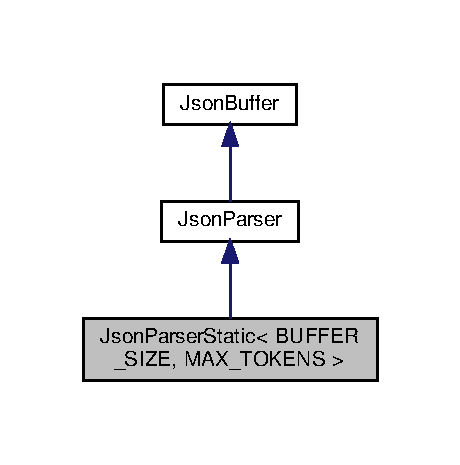
\includegraphics[width=221pt]{class_json_parser_static__inherit__graph}
\end{center}
\end{figure}


Collaboration diagram for Json\+Parser\+Static$<$ B\+U\+F\+F\+E\+R\+\_\+\+S\+I\+ZE, M\+A\+X\+\_\+\+T\+O\+K\+E\+NS $>$\+:
\nopagebreak
\begin{figure}[H]
\begin{center}
\leavevmode
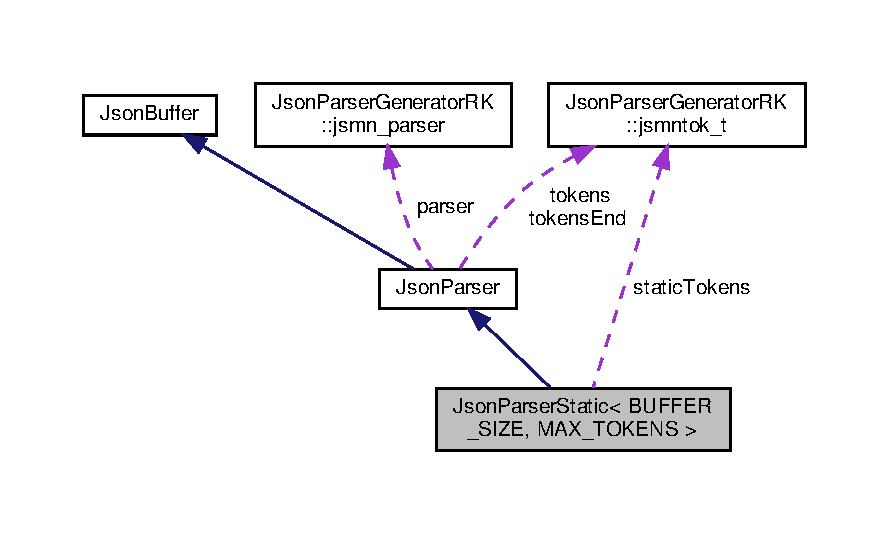
\includegraphics[width=350pt]{class_json_parser_static__coll__graph}
\end{center}
\end{figure}
\subsection*{Public Member Functions}
\begin{DoxyCompactItemize}
\item 
\hyperlink{class_json_parser_static_a6d0aa92ea003e383a1efa1a8533e1e60}{Json\+Parser\+Static} ()
\begin{DoxyCompactList}\small\item\em Construct a \hyperlink{class_json_parser}{Json\+Parser} using a static buffer and static maximum number of tokens. \end{DoxyCompactList}\end{DoxyCompactItemize}
\subsection*{Private Attributes}
\begin{DoxyCompactItemize}
\item 
char \hyperlink{class_json_parser_static_a7098ca786f3e7ecacbe2824e49c4fc23}{static\+Buffer} \mbox{[}B\+U\+F\+F\+E\+R\+\_\+\+S\+I\+ZE\mbox{]}
\begin{DoxyCompactList}\small\item\em The static buffer to hold the data. \end{DoxyCompactList}\item 
\hyperlink{struct_json_parser_generator_r_k_1_1jsmntok__t}{Json\+Parser\+Generator\+R\+K\+::jsmntok\+\_\+t} \hyperlink{class_json_parser_static_a46bd3b4c6e0d3205dfdcb6ef1e5dab8c}{static\+Tokens} \mbox{[}M\+A\+X\+\_\+\+T\+O\+K\+E\+NS\mbox{]}
\begin{DoxyCompactList}\small\item\em The static buffer to hold the tokens. \end{DoxyCompactList}\end{DoxyCompactItemize}
\subsection*{Additional Inherited Members}


\subsection{Detailed Description}
\subsubsection*{template$<$size\+\_\+t B\+U\+F\+F\+E\+R\+\_\+\+S\+I\+ZE, size\+\_\+t M\+A\+X\+\_\+\+T\+O\+K\+E\+NS$>$\newline
class Json\+Parser\+Static$<$ B\+U\+F\+F\+E\+R\+\_\+\+S\+I\+Z\+E, M\+A\+X\+\_\+\+T\+O\+K\+E\+N\+S $>$}

Creates a \hyperlink{class_json_parser}{Json\+Parser} with a static buffer. 

You normally use this when you\textquotesingle{}re creating a parser as a global variable. For small data (under around 256 bytes so) you can also allocate one on the stack.


\begin{DoxyParams}{Parameters}
{\em B\+U\+F\+F\+E\+R\+\_\+\+S\+I\+ZE} & The maximum size of the data to be parsed, in bytes. If you are parsing a webhook response split into parts, this is the total size of all parts.\\
\hline
{\em M\+A\+X\+\_\+\+T\+O\+K\+E\+NS} & The maximum number of tokens you expect. Each object has a token and two for each key/value pair. Each array is a token and one for each element in the array. \\
\hline
\end{DoxyParams}


Definition at line 772 of file Json\+Parser\+Generator\+R\+K.\+h.



\subsection{Constructor \& Destructor Documentation}
\mbox{\Hypertarget{class_json_parser_static_a6d0aa92ea003e383a1efa1a8533e1e60}\label{class_json_parser_static_a6d0aa92ea003e383a1efa1a8533e1e60}} 
\index{Json\+Parser\+Static@{Json\+Parser\+Static}!Json\+Parser\+Static@{Json\+Parser\+Static}}
\index{Json\+Parser\+Static@{Json\+Parser\+Static}!Json\+Parser\+Static@{Json\+Parser\+Static}}
\subsubsection{\texorpdfstring{Json\+Parser\+Static()}{JsonParserStatic()}}
{\footnotesize\ttfamily template$<$size\+\_\+t B\+U\+F\+F\+E\+R\+\_\+\+S\+I\+ZE, size\+\_\+t M\+A\+X\+\_\+\+T\+O\+K\+E\+NS$>$ \\
\hyperlink{class_json_parser_static}{Json\+Parser\+Static}$<$ B\+U\+F\+F\+E\+R\+\_\+\+S\+I\+ZE, M\+A\+X\+\_\+\+T\+O\+K\+E\+NS $>$\+::\hyperlink{class_json_parser_static}{Json\+Parser\+Static} (\begin{DoxyParamCaption}{ }\end{DoxyParamCaption})\hspace{0.3cm}{\ttfamily [inline]}, {\ttfamily [explicit]}}



Construct a \hyperlink{class_json_parser}{Json\+Parser} using a static buffer and static maximum number of tokens. 



Definition at line 777 of file Json\+Parser\+Generator\+R\+K.\+h.



\subsection{Member Data Documentation}
\mbox{\Hypertarget{class_json_parser_static_a7098ca786f3e7ecacbe2824e49c4fc23}\label{class_json_parser_static_a7098ca786f3e7ecacbe2824e49c4fc23}} 
\index{Json\+Parser\+Static@{Json\+Parser\+Static}!static\+Buffer@{static\+Buffer}}
\index{static\+Buffer@{static\+Buffer}!Json\+Parser\+Static@{Json\+Parser\+Static}}
\subsubsection{\texorpdfstring{static\+Buffer}{staticBuffer}}
{\footnotesize\ttfamily template$<$size\+\_\+t B\+U\+F\+F\+E\+R\+\_\+\+S\+I\+ZE, size\+\_\+t M\+A\+X\+\_\+\+T\+O\+K\+E\+NS$>$ \\
char \hyperlink{class_json_parser_static}{Json\+Parser\+Static}$<$ B\+U\+F\+F\+E\+R\+\_\+\+S\+I\+ZE, M\+A\+X\+\_\+\+T\+O\+K\+E\+NS $>$\+::static\+Buffer\mbox{[}B\+U\+F\+F\+E\+R\+\_\+\+S\+I\+ZE\mbox{]}\hspace{0.3cm}{\ttfamily [private]}}



The static buffer to hold the data. 



Definition at line 777 of file Json\+Parser\+Generator\+R\+K.\+h.

\mbox{\Hypertarget{class_json_parser_static_a46bd3b4c6e0d3205dfdcb6ef1e5dab8c}\label{class_json_parser_static_a46bd3b4c6e0d3205dfdcb6ef1e5dab8c}} 
\index{Json\+Parser\+Static@{Json\+Parser\+Static}!static\+Tokens@{static\+Tokens}}
\index{static\+Tokens@{static\+Tokens}!Json\+Parser\+Static@{Json\+Parser\+Static}}
\subsubsection{\texorpdfstring{static\+Tokens}{staticTokens}}
{\footnotesize\ttfamily template$<$size\+\_\+t B\+U\+F\+F\+E\+R\+\_\+\+S\+I\+ZE, size\+\_\+t M\+A\+X\+\_\+\+T\+O\+K\+E\+NS$>$ \\
\hyperlink{struct_json_parser_generator_r_k_1_1jsmntok__t}{Json\+Parser\+Generator\+R\+K\+::jsmntok\+\_\+t} \hyperlink{class_json_parser_static}{Json\+Parser\+Static}$<$ B\+U\+F\+F\+E\+R\+\_\+\+S\+I\+ZE, M\+A\+X\+\_\+\+T\+O\+K\+E\+NS $>$\+::static\+Tokens\mbox{[}M\+A\+X\+\_\+\+T\+O\+K\+E\+NS\mbox{]}\hspace{0.3cm}{\ttfamily [private]}}



The static buffer to hold the tokens. 



Definition at line 781 of file Json\+Parser\+Generator\+R\+K.\+h.



The documentation for this class was generated from the following file\+:\begin{DoxyCompactItemize}
\item 
lib/\+Json\+Parser\+Generator\+R\+K/src/\hyperlink{_json_parser_generator_r_k_8h}{Json\+Parser\+Generator\+R\+K.\+h}\end{DoxyCompactItemize}

\section{Json\+Parser\+String Class Reference}
\label{class_json_parser_string}\index{Json\+Parser\+String@{Json\+Parser\+String}}


Class used internally for writing to strings.  




{\ttfamily \#include $<$Json\+Parser\+Generator\+R\+K.\+h$>$}



Collaboration diagram for Json\+Parser\+String\+:\nopagebreak
\begin{figure}[H]
\begin{center}
\leavevmode
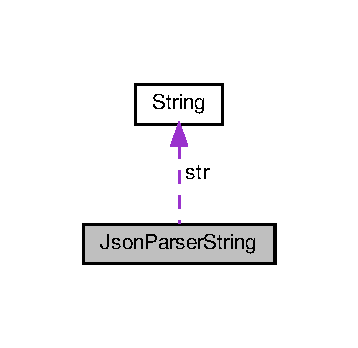
\includegraphics[width=172pt]{class_json_parser_string__coll__graph}
\end{center}
\end{figure}
\subsection*{Public Member Functions}
\begin{DoxyCompactItemize}
\item 
\textbf{ Json\+Parser\+String} (\textbf{ String} $\ast$\textbf{ str})
\begin{DoxyCompactList}\small\item\em Construct a \doxyref{Json\+Parser\+String}{p.}{class_json_parser_string} wrapping a Wiring \doxyref{String}{p.}{class_string}. \end{DoxyCompactList}\item 
\textbf{ Json\+Parser\+String} (char $\ast$\textbf{ buf}, size\+\_\+t \textbf{ buf\+Len})
\begin{DoxyCompactList}\small\item\em Construct a \doxyref{Json\+Parser\+String}{p.}{class_json_parser_string} wrapping a buffer and length. \end{DoxyCompactList}\item 
void \textbf{ append} (char ch)
\begin{DoxyCompactList}\small\item\em Append a single char to the underlying string. \end{DoxyCompactList}\item 
void \textbf{ append} (const char $\ast$\textbf{ str}, size\+\_\+t len)
\begin{DoxyCompactList}\small\item\em Append a buffer and length to the underlying string. \end{DoxyCompactList}\item 
size\+\_\+t \textbf{ get\+Length} () const
\begin{DoxyCompactList}\small\item\em Get the length of the string. \end{DoxyCompactList}\end{DoxyCompactItemize}
\subsection*{Protected Attributes}
\begin{DoxyCompactItemize}
\item 
\textbf{ String} $\ast$ \textbf{ str}
\begin{DoxyCompactList}\small\item\em When writing to a \doxyref{String}{p.}{class_string}, the \doxyref{String}{p.}{class_string} object. \end{DoxyCompactList}\item 
char $\ast$ \textbf{ buf}
\begin{DoxyCompactList}\small\item\em When writing to a buffer, the pointer to the buffer. Not used for \doxyref{String}{p.}{class_string}. \end{DoxyCompactList}\item 
size\+\_\+t \textbf{ buf\+Len}
\begin{DoxyCompactList}\small\item\em When writing to a buffer, the length of the buffer in bytes. Not used for \doxyref{String}{p.}{class_string}. \end{DoxyCompactList}\item 
size\+\_\+t \textbf{ length}
\begin{DoxyCompactList}\small\item\em The current offset being written to. \end{DoxyCompactList}\end{DoxyCompactItemize}


\subsection{Detailed Description}
Class used internally for writing to strings. 

This is a wrapper around either \doxyref{String}{p.}{class_string} (the Wiring version) or a buffer and length. This allows writing to a static buffer with no dynamic memory allocation at all.

One of the things about \doxyref{String}{p.}{class_string} is that while you can pre-\/allocate reserve space for data, you can\textquotesingle{}t get access to the internal length field, so you can\textquotesingle{}t write to raw bytes then resize it to the correct size. This wrapper is that allows appending to either a \doxyref{String}{p.}{class_string} or buffer to get around this limitation of \doxyref{String}{p.}{class_string}.

You can also use it for sizing only by passing N\+U\+LL for buf. 

Definition at line 92 of file Json\+Parser\+Generator\+R\+K.\+h.



\subsection{Constructor \& Destructor Documentation}
\mbox{\label{class_json_parser_string_a3942a87b6920b08e38ce01b4d4a41fc4}} 
\index{Json\+Parser\+String@{Json\+Parser\+String}!Json\+Parser\+String@{Json\+Parser\+String}}
\index{Json\+Parser\+String@{Json\+Parser\+String}!Json\+Parser\+String@{Json\+Parser\+String}}
\subsubsection{Json\+Parser\+String()\hspace{0.1cm}{\footnotesize\ttfamily [1/2]}}
{\footnotesize\ttfamily Json\+Parser\+String\+::\+Json\+Parser\+String (\begin{DoxyParamCaption}\item[{\textbf{ String} $\ast$}]{str }\end{DoxyParamCaption})}



Construct a \doxyref{Json\+Parser\+String}{p.}{class_json_parser_string} wrapping a Wiring \doxyref{String}{p.}{class_string}. 


\begin{DoxyParams}{Parameters}
{\em str} & A pointer Wiring \doxyref{String}{p.}{class_string} object to write to. \\
\hline
\end{DoxyParams}


Definition at line 623 of file Json\+Parser\+Generator\+R\+K.\+cpp.



References buf, buf\+Len, length, and str.



Referenced by Json\+Parser\+::get\+Token\+Json\+String(), and Json\+Parser\+::get\+Token\+Value().


\begin{DoxyCode}
623                                               : str(str), buf(0), bufLen(0), 
      length(0)\{
624 \}
\end{DoxyCode}
\mbox{\label{class_json_parser_string_ae0f9e3309682685ed259ad1370eb448f}} 
\index{Json\+Parser\+String@{Json\+Parser\+String}!Json\+Parser\+String@{Json\+Parser\+String}}
\index{Json\+Parser\+String@{Json\+Parser\+String}!Json\+Parser\+String@{Json\+Parser\+String}}
\subsubsection{Json\+Parser\+String()\hspace{0.1cm}{\footnotesize\ttfamily [2/2]}}
{\footnotesize\ttfamily Json\+Parser\+String\+::\+Json\+Parser\+String (\begin{DoxyParamCaption}\item[{char $\ast$}]{buf,  }\item[{size\+\_\+t}]{buf\+Len }\end{DoxyParamCaption})}



Construct a \doxyref{Json\+Parser\+String}{p.}{class_json_parser_string} wrapping a buffer and length. 


\begin{DoxyParams}{Parameters}
{\em buf} & A pointer to a buffer\\
\hline
{\em buf\+Len} & The length of the buffer in bytes \\
\hline
\end{DoxyParams}


Definition at line 626 of file Json\+Parser\+Generator\+R\+K.\+cpp.



References buf, buf\+Len, length, and str.



Referenced by Json\+Parser\+::get\+Token\+Json\+String(), and Json\+Parser\+::get\+Token\+Value().


\begin{DoxyCode}
626                                                            : str(0), buf(buf), 
      bufLen(bufLen), length(0)\{
627     \textcolor{keywordflow}{if} (buf && bufLen) \{
628         memset(buf, 0, bufLen);
629     \}
630 \}
\end{DoxyCode}


\subsection{Member Function Documentation}
\mbox{\label{class_json_parser_string_a7a8f809096c291c4cd7717df4a6534cf}} 
\index{Json\+Parser\+String@{Json\+Parser\+String}!append@{append}}
\index{append@{append}!Json\+Parser\+String@{Json\+Parser\+String}}
\subsubsection{append()\hspace{0.1cm}{\footnotesize\ttfamily [1/2]}}
{\footnotesize\ttfamily void Json\+Parser\+String\+::append (\begin{DoxyParamCaption}\item[{char}]{ch }\end{DoxyParamCaption})}



Append a single char to the underlying string. 


\begin{DoxyParams}{Parameters}
{\em ch} & The char to append. \\
\hline
\end{DoxyParams}


Definition at line 632 of file Json\+Parser\+Generator\+R\+K.\+cpp.



References buf, buf\+Len, String\+::concat(), length, and str.



Referenced by append(), Json\+Parser\+::append\+Utf8(), and Json\+Parser\+::get\+Token\+Value().


\begin{DoxyCode}
632                                      \{
633     \textcolor{keywordflow}{if} (str) \{
634         str->concat(ch);
635         length++;
636     \}
637     \textcolor{keywordflow}{else} \{
638         \textcolor{keywordflow}{if} (buf && length < (bufLen - 1)) \{
639             buf[length] = ch;
640         \}
641         length++;
642     \}
643 \}
\end{DoxyCode}
\mbox{\label{class_json_parser_string_a28e2858fe1481e20fa8bc40054378c9f}} 
\index{Json\+Parser\+String@{Json\+Parser\+String}!append@{append}}
\index{append@{append}!Json\+Parser\+String@{Json\+Parser\+String}}
\subsubsection{append()\hspace{0.1cm}{\footnotesize\ttfamily [2/2]}}
{\footnotesize\ttfamily void Json\+Parser\+String\+::append (\begin{DoxyParamCaption}\item[{const char $\ast$}]{str,  }\item[{size\+\_\+t}]{len }\end{DoxyParamCaption})}



Append a buffer and length to the underlying string. 


\begin{DoxyParams}{Parameters}
{\em str} & A pointer to the character to add. Does not need to be null-\/terminated.\\
\hline
{\em len} & Length of the string to append in bytes. \\
\hline
\end{DoxyParams}


Definition at line 645 of file Json\+Parser\+Generator\+R\+K.\+cpp.



References append().



Referenced by Json\+Parser\+::get\+Token\+Json\+String().


\begin{DoxyCode}
645                                                          \{
646     \textcolor{keywordflow}{for}(\textcolor{keywordtype}{size\_t} ii = 0; ii < len; ii++) \{
647         append(str[ii]);
648     \}
649 \}
\end{DoxyCode}
\mbox{\label{class_json_parser_string_a3a495e1fb69d2900fda8b0556c93e51c}} 
\index{Json\+Parser\+String@{Json\+Parser\+String}!get\+Length@{get\+Length}}
\index{get\+Length@{get\+Length}!Json\+Parser\+String@{Json\+Parser\+String}}
\subsubsection{get\+Length()}
{\footnotesize\ttfamily size\+\_\+t Json\+Parser\+String\+::get\+Length (\begin{DoxyParamCaption}{ }\end{DoxyParamCaption}) const\hspace{0.3cm}{\ttfamily [inline]}}



Get the length of the string. 

\begin{DoxyReturn}{Returns}
The string length in bytes. If the string contains U\+T\+F-\/8 characters, it will be the number of bytes, not characters.
\end{DoxyReturn}
For buffer and buf\+Lenb, the maximum string length will be buf\+Len -\/ 1 to leave room for the null terminator. 

Definition at line 134 of file Json\+Parser\+Generator\+R\+K.\+h.



References length.



Referenced by Json\+Parser\+::get\+Token\+Json\+String(), and Json\+Parser\+::get\+Token\+Value().


\begin{DoxyCode}
134 \{ \textcolor{keywordflow}{return} length; \}
\end{DoxyCode}


\subsection{Member Data Documentation}
\mbox{\label{class_json_parser_string_a3ffd87df1aff38ff4142fad32e1e3de0}} 
\index{Json\+Parser\+String@{Json\+Parser\+String}!buf@{buf}}
\index{buf@{buf}!Json\+Parser\+String@{Json\+Parser\+String}}
\subsubsection{buf}
{\footnotesize\ttfamily char$\ast$ Json\+Parser\+String\+::buf\hspace{0.3cm}{\ttfamily [protected]}}



When writing to a buffer, the pointer to the buffer. Not used for \doxyref{String}{p.}{class_string}. 



Definition at line 138 of file Json\+Parser\+Generator\+R\+K.\+h.



Referenced by append(), and Json\+Parser\+String().

\mbox{\label{class_json_parser_string_a376957bb37fc229f44d0d85ce74adb4a}} 
\index{Json\+Parser\+String@{Json\+Parser\+String}!buf\+Len@{buf\+Len}}
\index{buf\+Len@{buf\+Len}!Json\+Parser\+String@{Json\+Parser\+String}}
\subsubsection{buf\+Len}
{\footnotesize\ttfamily size\+\_\+t Json\+Parser\+String\+::buf\+Len\hspace{0.3cm}{\ttfamily [protected]}}



When writing to a buffer, the length of the buffer in bytes. Not used for \doxyref{String}{p.}{class_string}. 



Definition at line 139 of file Json\+Parser\+Generator\+R\+K.\+h.



Referenced by append(), and Json\+Parser\+String().

\mbox{\label{class_json_parser_string_a2b3a350599c49f6e7e368fc8b508cf6f}} 
\index{Json\+Parser\+String@{Json\+Parser\+String}!length@{length}}
\index{length@{length}!Json\+Parser\+String@{Json\+Parser\+String}}
\subsubsection{length}
{\footnotesize\ttfamily size\+\_\+t Json\+Parser\+String\+::length\hspace{0.3cm}{\ttfamily [protected]}}



The current offset being written to. 



Definition at line 140 of file Json\+Parser\+Generator\+R\+K.\+h.



Referenced by append(), get\+Length(), and Json\+Parser\+String().

\mbox{\label{class_json_parser_string_ac98659ff5a56537979b6c60d28648224}} 
\index{Json\+Parser\+String@{Json\+Parser\+String}!str@{str}}
\index{str@{str}!Json\+Parser\+String@{Json\+Parser\+String}}
\subsubsection{str}
{\footnotesize\ttfamily \textbf{ String}$\ast$ Json\+Parser\+String\+::str\hspace{0.3cm}{\ttfamily [protected]}}



When writing to a \doxyref{String}{p.}{class_string}, the \doxyref{String}{p.}{class_string} object. 



Definition at line 137 of file Json\+Parser\+Generator\+R\+K.\+h.



Referenced by append(), and Json\+Parser\+String().



The documentation for this class was generated from the following files\+:\begin{DoxyCompactItemize}
\item 
lib/\+Json\+Parser\+Generator\+R\+K/src/\textbf{ Json\+Parser\+Generator\+R\+K.\+h}\item 
lib/\+Json\+Parser\+Generator\+R\+K/src/\textbf{ Json\+Parser\+Generator\+R\+K.\+cpp}\end{DoxyCompactItemize}

\hypertarget{class_json_reference}{}\section{Json\+Reference Class Reference}
\label{class_json_reference}\index{Json\+Reference@{Json\+Reference}}


This class provides a fluent-\/style A\+PI for easily traversing a tree of J\+S\+ON objects to find a value.  




{\ttfamily \#include $<$Json\+Parser\+Generator\+R\+K.\+h$>$}



Collaboration diagram for Json\+Reference\+:\nopagebreak
\begin{figure}[H]
\begin{center}
\leavevmode
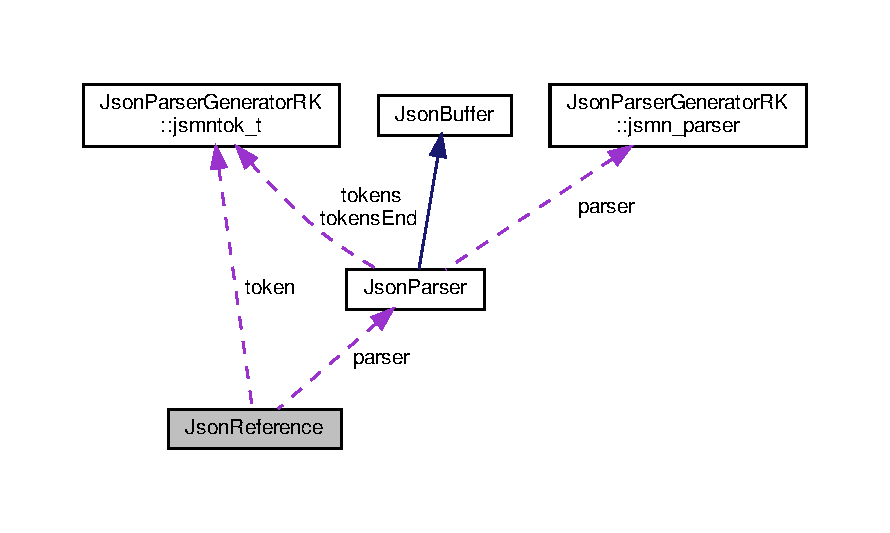
\includegraphics[width=350pt]{class_json_reference__coll__graph}
\end{center}
\end{figure}
\subsection*{Public Member Functions}
\begin{DoxyCompactItemize}
\item 
\hyperlink{class_json_reference_aa4d71b4a5c47270192b92b23b20ca149}{Json\+Reference} (const \hyperlink{class_json_parser}{Json\+Parser} $\ast$\hyperlink{class_json_reference_a37fb436fae63e7e452fc2325eddf3e8b}{parser})
\begin{DoxyCompactList}\small\item\em Constructs an object. Normally you use the \hyperlink{class_json_parser}{Json\+Parser} get\+Reference() method to get one of these instead of constructing one. \end{DoxyCompactList}\item 
virtual \hyperlink{class_json_reference_a4aca0aedf85a69c53d3af71baaee5030}{$\sim$\+Json\+Reference} ()
\begin{DoxyCompactList}\small\item\em Destructor. This does not affect the lifecycle of the \hyperlink{class_json_parser}{Json\+Parser}. \end{DoxyCompactList}\item 
\hyperlink{class_json_reference_a9b1d0b53240a31cd66918b76ffbfac61}{Json\+Reference} (const \hyperlink{class_json_parser}{Json\+Parser} $\ast$\hyperlink{class_json_reference_a37fb436fae63e7e452fc2325eddf3e8b}{parser}, const \hyperlink{struct_json_parser_generator_r_k_1_1jsmntok__t}{Json\+Parser\+Generator\+R\+K\+::jsmntok\+\_\+t} $\ast$\hyperlink{class_json_reference_a895a16fb8f781504fe39efd194ed5232}{token})
\begin{DoxyCompactList}\small\item\em Constructs are \hyperlink{class_json_reference}{Json\+Reference} for a specific token within a \hyperlink{class_json_parser}{Json\+Parser}. \end{DoxyCompactList}\item 
\hyperlink{class_json_reference}{Json\+Reference} \hyperlink{class_json_reference_abb7263eb5a84a137f0ed45631993d171}{key} (const char $\ast$name) const
\begin{DoxyCompactList}\small\item\em For \hyperlink{class_json_reference}{Json\+Reference} that refers to a J\+S\+ON object, gets a new \hyperlink{class_json_reference}{Json\+Reference} to a value with the specified key name. \end{DoxyCompactList}\item 
\hyperlink{class_json_reference}{Json\+Reference} \hyperlink{class_json_reference_aecf18512e22e7efeba7572072576e09e}{index} (size\+\_\+t index) const
\begin{DoxyCompactList}\small\item\em For a \hyperlink{class_json_reference}{Json\+Reference} that refers to a J\+S\+ON array, gets a new \hyperlink{class_json_reference}{Json\+Reference} to a value in the array by index. \end{DoxyCompactList}\item 
size\+\_\+t \hyperlink{class_json_reference_a9a196b64764b2943c425cee334f0b999}{size} () const
\begin{DoxyCompactList}\small\item\em For a \hyperlink{class_json_reference}{Json\+Reference} that refers to a J\+S\+ON array, gets the size of the array. \end{DoxyCompactList}\item 
{\footnotesize template$<$class T $>$ }\\bool \hyperlink{class_json_reference_a9eb0bbb4ed98e7ebceeb41c757e0f15b}{value} (T \&result) const
\begin{DoxyCompactList}\small\item\em Get a value of the specified type for a given value for a specified key, or index for an array. \end{DoxyCompactList}\item 
bool \hyperlink{class_json_reference_a45d8e15942d4f3cf79e6e7d0c9218acf}{value\+Bool} (bool default\+Value=false) const
\begin{DoxyCompactList}\small\item\em Returns a boolean (bool) value for an object value for key, or array index. \end{DoxyCompactList}\item 
int \hyperlink{class_json_reference_afcf4b05a4b789ca1ea938a1adb33cafa}{value\+Int} (int default\+Value=0) const
\begin{DoxyCompactList}\small\item\em Returns a integer (int) value for an object value for key, or array index. \end{DoxyCompactList}\item 
unsigned long \hyperlink{class_json_reference_a081b56c80097d802911610fb17253211}{value\+Unsigned\+Long} (unsigned long default\+Value=0) const
\begin{DoxyCompactList}\small\item\em Returns a unsigned long integer for an object value for key, or array index. \end{DoxyCompactList}\item 
float \hyperlink{class_json_reference_afa346d628f8ecb4ad2b7a67c7634a85c}{value\+Float} (float default\+Value=0.\+0) const
\begin{DoxyCompactList}\small\item\em Returns a float value for an object value for key, or array index. \end{DoxyCompactList}\item 
double \hyperlink{class_json_reference_a670c3313ff8bc1399ce0a6efdad3b0db}{value\+Double} (double default\+Value=0.\+0) const
\begin{DoxyCompactList}\small\item\em Returns a double value for an object value for key, or array index. \end{DoxyCompactList}\item 
\hyperlink{class_string}{String} \hyperlink{class_json_reference_ab9dfec23570193b9ab1d16b07fba6022}{value\+String} () const
\begin{DoxyCompactList}\small\item\em Returns a \hyperlink{class_string}{String} value for an object value for key, or array index. \end{DoxyCompactList}\end{DoxyCompactItemize}
\subsection*{Private Attributes}
\begin{DoxyCompactItemize}
\item 
const \hyperlink{class_json_parser}{Json\+Parser} $\ast$ \hyperlink{class_json_reference_a37fb436fae63e7e452fc2325eddf3e8b}{parser}
\item 
const \hyperlink{struct_json_parser_generator_r_k_1_1jsmntok__t}{Json\+Parser\+Generator\+R\+K\+::jsmntok\+\_\+t} $\ast$ \hyperlink{class_json_reference_a895a16fb8f781504fe39efd194ed5232}{token}
\end{DoxyCompactItemize}


\subsection{Detailed Description}
This class provides a fluent-\/style A\+PI for easily traversing a tree of J\+S\+ON objects to find a value. 

Definition at line 788 of file Json\+Parser\+Generator\+R\+K.\+h.



\subsection{Constructor \& Destructor Documentation}
\mbox{\Hypertarget{class_json_reference_aa4d71b4a5c47270192b92b23b20ca149}\label{class_json_reference_aa4d71b4a5c47270192b92b23b20ca149}} 
\index{Json\+Reference@{Json\+Reference}!Json\+Reference@{Json\+Reference}}
\index{Json\+Reference@{Json\+Reference}!Json\+Reference@{Json\+Reference}}
\subsubsection{\texorpdfstring{Json\+Reference()}{JsonReference()}\hspace{0.1cm}{\footnotesize\ttfamily [1/2]}}
{\footnotesize\ttfamily Json\+Reference\+::\+Json\+Reference (\begin{DoxyParamCaption}\item[{const \hyperlink{class_json_parser}{Json\+Parser} $\ast$}]{parser }\end{DoxyParamCaption})}



Constructs an object. Normally you use the \hyperlink{class_json_parser}{Json\+Parser} get\+Reference() method to get one of these instead of constructing one. 


\begin{DoxyParams}{Parameters}
{\em parser} & The \hyperlink{class_json_parser}{Json\+Parser} object you\textquotesingle{}re traversing \\
\hline
\end{DoxyParams}


Definition at line 546 of file Json\+Parser\+Generator\+R\+K.\+cpp.



References parser, and token.



Referenced by Json\+Parser\+::get\+Reference(), index(), and key().

\mbox{\Hypertarget{class_json_reference_a4aca0aedf85a69c53d3af71baaee5030}\label{class_json_reference_a4aca0aedf85a69c53d3af71baaee5030}} 
\index{Json\+Reference@{Json\+Reference}!````~Json\+Reference@{$\sim$\+Json\+Reference}}
\index{````~Json\+Reference@{$\sim$\+Json\+Reference}!Json\+Reference@{Json\+Reference}}
\subsubsection{\texorpdfstring{$\sim$\+Json\+Reference()}{~JsonReference()}}
{\footnotesize\ttfamily Json\+Reference\+::$\sim$\+Json\+Reference (\begin{DoxyParamCaption}{ }\end{DoxyParamCaption})\hspace{0.3cm}{\ttfamily [virtual]}}



Destructor. This does not affect the lifecycle of the \hyperlink{class_json_parser}{Json\+Parser}. 



Definition at line 550 of file Json\+Parser\+Generator\+R\+K.\+cpp.

\mbox{\Hypertarget{class_json_reference_a9b1d0b53240a31cd66918b76ffbfac61}\label{class_json_reference_a9b1d0b53240a31cd66918b76ffbfac61}} 
\index{Json\+Reference@{Json\+Reference}!Json\+Reference@{Json\+Reference}}
\index{Json\+Reference@{Json\+Reference}!Json\+Reference@{Json\+Reference}}
\subsubsection{\texorpdfstring{Json\+Reference()}{JsonReference()}\hspace{0.1cm}{\footnotesize\ttfamily [2/2]}}
{\footnotesize\ttfamily Json\+Reference\+::\+Json\+Reference (\begin{DoxyParamCaption}\item[{const \hyperlink{class_json_parser}{Json\+Parser} $\ast$}]{parser,  }\item[{const \hyperlink{struct_json_parser_generator_r_k_1_1jsmntok__t}{Json\+Parser\+Generator\+R\+K\+::jsmntok\+\_\+t} $\ast$}]{token }\end{DoxyParamCaption})}



Constructs are \hyperlink{class_json_reference}{Json\+Reference} for a specific token within a \hyperlink{class_json_parser}{Json\+Parser}. 



Definition at line 553 of file Json\+Parser\+Generator\+R\+K.\+cpp.



References parser, and token.



Referenced by Json\+Parser\+::get\+Reference(), index(), and key().



\subsection{Member Function Documentation}
\mbox{\Hypertarget{class_json_reference_aecf18512e22e7efeba7572072576e09e}\label{class_json_reference_aecf18512e22e7efeba7572072576e09e}} 
\index{Json\+Reference@{Json\+Reference}!index@{index}}
\index{index@{index}!Json\+Reference@{Json\+Reference}}
\subsubsection{\texorpdfstring{index()}{index()}}
{\footnotesize\ttfamily \hyperlink{class_json_reference}{Json\+Reference} Json\+Reference\+::index (\begin{DoxyParamCaption}\item[{size\+\_\+t}]{index }\end{DoxyParamCaption}) const}



For a \hyperlink{class_json_reference}{Json\+Reference} that refers to a J\+S\+ON array, gets a new \hyperlink{class_json_reference}{Json\+Reference} to a value in the array by index. 


\begin{DoxyParams}{Parameters}
{\em index} & The index to retrieve (0 = first item, 1 = second item, ...).\\
\hline
\end{DoxyParams}
\begin{DoxyReturn}{Returns}
A \hyperlink{class_json_reference}{Json\+Reference} to the value for this index. 
\end{DoxyReturn}


Definition at line 567 of file Json\+Parser\+Generator\+R\+K.\+cpp.



References Json\+Parser\+::get\+Value\+Token\+By\+Index(), Json\+Reference(), parser, and token.



Referenced by main().

\mbox{\Hypertarget{class_json_reference_abb7263eb5a84a137f0ed45631993d171}\label{class_json_reference_abb7263eb5a84a137f0ed45631993d171}} 
\index{Json\+Reference@{Json\+Reference}!key@{key}}
\index{key@{key}!Json\+Reference@{Json\+Reference}}
\subsubsection{\texorpdfstring{key()}{key()}}
{\footnotesize\ttfamily \hyperlink{class_json_reference}{Json\+Reference} Json\+Reference\+::key (\begin{DoxyParamCaption}\item[{const char $\ast$}]{name }\end{DoxyParamCaption}) const}



For \hyperlink{class_json_reference}{Json\+Reference} that refers to a J\+S\+ON object, gets a new \hyperlink{class_json_reference}{Json\+Reference} to a value with the specified key name. 


\begin{DoxyParams}{Parameters}
{\em name} & of the key to look for.\\
\hline
\end{DoxyParams}
\begin{DoxyReturn}{Returns}
A \hyperlink{class_json_reference}{Json\+Reference} to the value for this key. 
\end{DoxyReturn}


Definition at line 556 of file Json\+Parser\+Generator\+R\+K.\+cpp.



References Json\+Parser\+::get\+Value\+Token\+By\+Key(), Json\+Reference(), parser, and token.



Referenced by main().

\mbox{\Hypertarget{class_json_reference_a9a196b64764b2943c425cee334f0b999}\label{class_json_reference_a9a196b64764b2943c425cee334f0b999}} 
\index{Json\+Reference@{Json\+Reference}!size@{size}}
\index{size@{size}!Json\+Reference@{Json\+Reference}}
\subsubsection{\texorpdfstring{size()}{size()}}
{\footnotesize\ttfamily size\+\_\+t Json\+Reference\+::size (\begin{DoxyParamCaption}{ }\end{DoxyParamCaption}) const}



For a \hyperlink{class_json_reference}{Json\+Reference} that refers to a J\+S\+ON array, gets the size of the array. 

\begin{DoxyReturn}{Returns}
0 = an empty array, 1 = one element, ... 
\end{DoxyReturn}


Definition at line 578 of file Json\+Parser\+Generator\+R\+K.\+cpp.



References Json\+Parser\+::get\+Array\+Size(), parser, and token.



Referenced by main().

\mbox{\Hypertarget{class_json_reference_a9eb0bbb4ed98e7ebceeb41c757e0f15b}\label{class_json_reference_a9eb0bbb4ed98e7ebceeb41c757e0f15b}} 
\index{Json\+Reference@{Json\+Reference}!value@{value}}
\index{value@{value}!Json\+Reference@{Json\+Reference}}
\subsubsection{\texorpdfstring{value()}{value()}}
{\footnotesize\ttfamily template$<$class T $>$ \\
bool Json\+Reference\+::value (\begin{DoxyParamCaption}\item[{T \&}]{result }\end{DoxyParamCaption}) const\hspace{0.3cm}{\ttfamily [inline]}}



Get a value of the specified type for a given value for a specified key, or index for an array. 


\begin{DoxyParams}{Parameters}
{\em result} & Filled in with the value. The value can be of type\+: bool, int, unsigned long, float, double, \hyperlink{class_string}{String}, or (char $\ast$, size\+\_\+t\&).\\
\hline
\end{DoxyParams}
There are also type-\/specific versions like value\+Bool that return the value, instead of having to pass an object to hold the value, as in this call. 

Definition at line 843 of file Json\+Parser\+Generator\+R\+K.\+h.



References parser, and token.



Referenced by value\+Bool(), value\+Double(), value\+Float(), value\+Int(), value\+String(), and value\+Unsigned\+Long().

\mbox{\Hypertarget{class_json_reference_a45d8e15942d4f3cf79e6e7d0c9218acf}\label{class_json_reference_a45d8e15942d4f3cf79e6e7d0c9218acf}} 
\index{Json\+Reference@{Json\+Reference}!value\+Bool@{value\+Bool}}
\index{value\+Bool@{value\+Bool}!Json\+Reference@{Json\+Reference}}
\subsubsection{\texorpdfstring{value\+Bool()}{valueBool()}}
{\footnotesize\ttfamily bool Json\+Reference\+::value\+Bool (\begin{DoxyParamCaption}\item[{bool}]{default\+Value = {\ttfamily false} }\end{DoxyParamCaption}) const}



Returns a boolean (bool) value for an object value for key, or array index. 


\begin{DoxyParams}{Parameters}
{\em default\+Value} & Optional value to use if the key or array index is not found. Default\+: false. \\
\hline
\end{DoxyParams}


Definition at line 587 of file Json\+Parser\+Generator\+R\+K.\+cpp.



References value().

\mbox{\Hypertarget{class_json_reference_a670c3313ff8bc1399ce0a6efdad3b0db}\label{class_json_reference_a670c3313ff8bc1399ce0a6efdad3b0db}} 
\index{Json\+Reference@{Json\+Reference}!value\+Double@{value\+Double}}
\index{value\+Double@{value\+Double}!Json\+Reference@{Json\+Reference}}
\subsubsection{\texorpdfstring{value\+Double()}{valueDouble()}}
{\footnotesize\ttfamily double Json\+Reference\+::value\+Double (\begin{DoxyParamCaption}\item[{double}]{default\+Value = {\ttfamily 0.0} }\end{DoxyParamCaption}) const}



Returns a double value for an object value for key, or array index. 


\begin{DoxyParams}{Parameters}
{\em default\+Value} & Optional value to use if the key or array index is not found. Default\+: 0.\+0. \\
\hline
\end{DoxyParams}


Definition at line 607 of file Json\+Parser\+Generator\+R\+K.\+cpp.



References value().



Referenced by main().

\mbox{\Hypertarget{class_json_reference_afa346d628f8ecb4ad2b7a67c7634a85c}\label{class_json_reference_afa346d628f8ecb4ad2b7a67c7634a85c}} 
\index{Json\+Reference@{Json\+Reference}!value\+Float@{value\+Float}}
\index{value\+Float@{value\+Float}!Json\+Reference@{Json\+Reference}}
\subsubsection{\texorpdfstring{value\+Float()}{valueFloat()}}
{\footnotesize\ttfamily float Json\+Reference\+::value\+Float (\begin{DoxyParamCaption}\item[{float}]{default\+Value = {\ttfamily 0.0} }\end{DoxyParamCaption}) const}



Returns a float value for an object value for key, or array index. 


\begin{DoxyParams}{Parameters}
{\em default\+Value} & Optional value to use if the key or array index is not found. Default\+: 0.\+0. \\
\hline
\end{DoxyParams}


Definition at line 602 of file Json\+Parser\+Generator\+R\+K.\+cpp.



References value().



Referenced by main().

\mbox{\Hypertarget{class_json_reference_afcf4b05a4b789ca1ea938a1adb33cafa}\label{class_json_reference_afcf4b05a4b789ca1ea938a1adb33cafa}} 
\index{Json\+Reference@{Json\+Reference}!value\+Int@{value\+Int}}
\index{value\+Int@{value\+Int}!Json\+Reference@{Json\+Reference}}
\subsubsection{\texorpdfstring{value\+Int()}{valueInt()}}
{\footnotesize\ttfamily int Json\+Reference\+::value\+Int (\begin{DoxyParamCaption}\item[{int}]{default\+Value = {\ttfamily 0} }\end{DoxyParamCaption}) const}



Returns a integer (int) value for an object value for key, or array index. 


\begin{DoxyParams}{Parameters}
{\em default\+Value} & Optional value to use if the key or array index is not found. Default\+: 0. \\
\hline
\end{DoxyParams}


Definition at line 592 of file Json\+Parser\+Generator\+R\+K.\+cpp.



References value().



Referenced by main().

\mbox{\Hypertarget{class_json_reference_ab9dfec23570193b9ab1d16b07fba6022}\label{class_json_reference_ab9dfec23570193b9ab1d16b07fba6022}} 
\index{Json\+Reference@{Json\+Reference}!value\+String@{value\+String}}
\index{value\+String@{value\+String}!Json\+Reference@{Json\+Reference}}
\subsubsection{\texorpdfstring{value\+String()}{valueString()}}
{\footnotesize\ttfamily \hyperlink{class_string}{String} Json\+Reference\+::value\+String (\begin{DoxyParamCaption}{ }\end{DoxyParamCaption}) const}



Returns a \hyperlink{class_string}{String} value for an object value for key, or array index. 

\begin{DoxyReturn}{Returns}
The string value, or an empty string if the key or array index is not found. 
\end{DoxyReturn}


Definition at line 612 of file Json\+Parser\+Generator\+R\+K.\+cpp.



References value().



Referenced by main().

\mbox{\Hypertarget{class_json_reference_a081b56c80097d802911610fb17253211}\label{class_json_reference_a081b56c80097d802911610fb17253211}} 
\index{Json\+Reference@{Json\+Reference}!value\+Unsigned\+Long@{value\+Unsigned\+Long}}
\index{value\+Unsigned\+Long@{value\+Unsigned\+Long}!Json\+Reference@{Json\+Reference}}
\subsubsection{\texorpdfstring{value\+Unsigned\+Long()}{valueUnsignedLong()}}
{\footnotesize\ttfamily unsigned long Json\+Reference\+::value\+Unsigned\+Long (\begin{DoxyParamCaption}\item[{unsigned long}]{default\+Value = {\ttfamily 0} }\end{DoxyParamCaption}) const}



Returns a unsigned long integer for an object value for key, or array index. 


\begin{DoxyParams}{Parameters}
{\em default\+Value} & Optional value to use if the key or array index is not found. Default\+: 0. \\
\hline
\end{DoxyParams}


Definition at line 597 of file Json\+Parser\+Generator\+R\+K.\+cpp.



References value().



Referenced by main().



\subsection{Member Data Documentation}
\mbox{\Hypertarget{class_json_reference_a37fb436fae63e7e452fc2325eddf3e8b}\label{class_json_reference_a37fb436fae63e7e452fc2325eddf3e8b}} 
\index{Json\+Reference@{Json\+Reference}!parser@{parser}}
\index{parser@{parser}!Json\+Reference@{Json\+Reference}}
\subsubsection{\texorpdfstring{parser}{parser}}
{\footnotesize\ttfamily const \hyperlink{class_json_parser}{Json\+Parser}$\ast$ Json\+Reference\+::parser\hspace{0.3cm}{\ttfamily [private]}}



Definition at line 895 of file Json\+Parser\+Generator\+R\+K.\+h.



Referenced by index(), Json\+Reference(), key(), size(), and value().

\mbox{\Hypertarget{class_json_reference_a895a16fb8f781504fe39efd194ed5232}\label{class_json_reference_a895a16fb8f781504fe39efd194ed5232}} 
\index{Json\+Reference@{Json\+Reference}!token@{token}}
\index{token@{token}!Json\+Reference@{Json\+Reference}}
\subsubsection{\texorpdfstring{token}{token}}
{\footnotesize\ttfamily const \hyperlink{struct_json_parser_generator_r_k_1_1jsmntok__t}{Json\+Parser\+Generator\+R\+K\+::jsmntok\+\_\+t}$\ast$ Json\+Reference\+::token\hspace{0.3cm}{\ttfamily [private]}}



Definition at line 896 of file Json\+Parser\+Generator\+R\+K.\+h.



Referenced by index(), Json\+Reference(), key(), size(), and value().



The documentation for this class was generated from the following files\+:\begin{DoxyCompactItemize}
\item 
lib/\+Json\+Parser\+Generator\+R\+K/src/\hyperlink{_json_parser_generator_r_k_8h}{Json\+Parser\+Generator\+R\+K.\+h}\item 
lib/\+Json\+Parser\+Generator\+R\+K/src/\hyperlink{_json_parser_generator_r_k_8cpp}{Json\+Parser\+Generator\+R\+K.\+cpp}\end{DoxyCompactItemize}

\section{Json\+Writer Class Reference}
\label{class_json_writer}\index{Json\+Writer@{Json\+Writer}}


Class for building a J\+S\+ON string.  




{\ttfamily \#include $<$Json\+Parser\+Generator\+R\+K.\+h$>$}



Inheritance diagram for Json\+Writer\+:\nopagebreak
\begin{figure}[H]
\begin{center}
\leavevmode
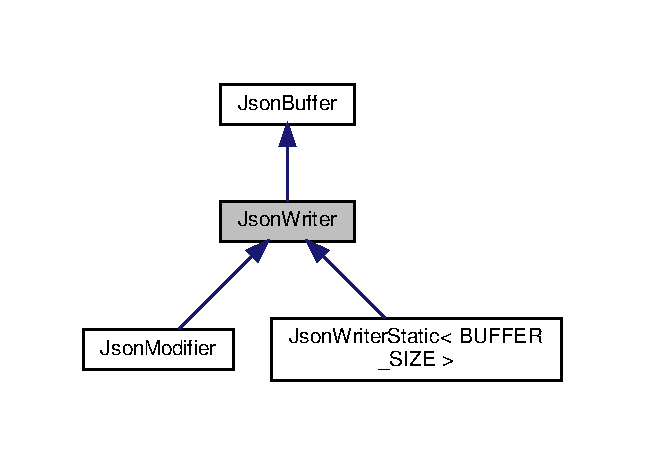
\includegraphics[width=310pt]{class_json_writer__inherit__graph}
\end{center}
\end{figure}


Collaboration diagram for Json\+Writer\+:\nopagebreak
\begin{figure}[H]
\begin{center}
\leavevmode
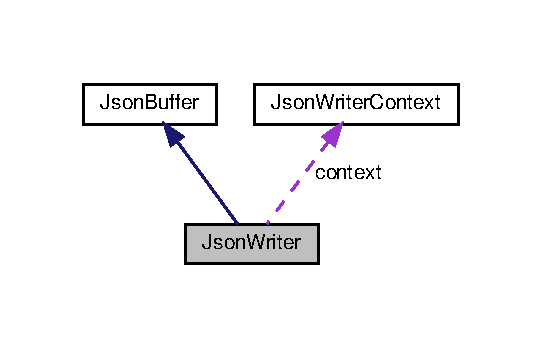
\includegraphics[width=260pt]{class_json_writer__coll__graph}
\end{center}
\end{figure}
\subsection*{Public Member Functions}
\begin{DoxyCompactItemize}
\item 
\textbf{ Json\+Writer} ()
\begin{DoxyCompactList}\small\item\em Construct a \doxyref{Json\+Writer}{p.}{class_json_writer} with a dynamically allocated buffer. \end{DoxyCompactList}\item 
virtual \textbf{ $\sim$\+Json\+Writer} ()
\begin{DoxyCompactList}\small\item\em Destroy the object. If the buffer was dynamically allocated it will be freed. \end{DoxyCompactList}\item 
\textbf{ Json\+Writer} (char $\ast$\textbf{ buffer}, size\+\_\+t \textbf{ buffer\+Len})
\begin{DoxyCompactList}\small\item\em Construct a \doxyref{Json\+Writer}{p.}{class_json_writer} to write to a static buffer. \end{DoxyCompactList}\item 
void \textbf{ init} ()
\begin{DoxyCompactList}\small\item\em Reset the writer, clearing all data. \end{DoxyCompactList}\item 
bool \textbf{ start\+Object} ()
\begin{DoxyCompactList}\small\item\em Start a new J\+S\+ON object. Make sure you finish it with \doxyref{finish\+Object\+Or\+Array()}{p.}{class_json_writer_adbd96b46b0679bea3a066c0e62bd86b0} \end{DoxyCompactList}\item 
bool \textbf{ start\+Array} ()
\begin{DoxyCompactList}\small\item\em Start a new J\+S\+ON array. Make sure you finish it with \doxyref{finish\+Object\+Or\+Array()}{p.}{class_json_writer_adbd96b46b0679bea3a066c0e62bd86b0} \end{DoxyCompactList}\item 
void \textbf{ finish\+Object\+Or\+Array} ()
\begin{DoxyCompactList}\small\item\em Finsh an object or array started with \doxyref{start\+Object()}{p.}{class_json_writer_a43d1a78bf211a2f12cfe9253462717ae} or \doxyref{start\+Array()}{p.}{class_json_writer_a7ccfcbf66a8ed9a2728e6f6ae4b705ec} \end{DoxyCompactList}\item 
void \textbf{ insert\+Value} (bool value)
\begin{DoxyCompactList}\small\item\em Inserts a boolean value (\char`\"{}true\char`\"{} or \char`\"{}false\char`\"{}). \end{DoxyCompactList}\item 
void \textbf{ insert\+Value} (int value)
\begin{DoxyCompactList}\small\item\em Inserts an integer value. \end{DoxyCompactList}\item 
void \textbf{ insert\+Value} (unsigned int value)
\begin{DoxyCompactList}\small\item\em Inserts an unsigned integer value. \end{DoxyCompactList}\item 
void \textbf{ insert\+Value} (long value)
\begin{DoxyCompactList}\small\item\em Inserts a long integer value. \end{DoxyCompactList}\item 
void \textbf{ insert\+Value} (unsigned long value)
\begin{DoxyCompactList}\small\item\em Inserts an unsigned long integer value. \end{DoxyCompactList}\item 
void \textbf{ insert\+Value} (float value)
\begin{DoxyCompactList}\small\item\em Inserts a floating point value. \end{DoxyCompactList}\item 
void \textbf{ insert\+Value} (double value)
\begin{DoxyCompactList}\small\item\em Inserts a floating point double value. \end{DoxyCompactList}\item 
void \textbf{ insert\+Value} (const char $\ast$value)
\begin{DoxyCompactList}\small\item\em Inserts a quoted string value. This escapes special characters and encodes utf-\/8. \end{DoxyCompactList}\item 
void \textbf{ insert\+Value} (const \textbf{ String} \&value)
\begin{DoxyCompactList}\small\item\em Inserts a quoted string value. \end{DoxyCompactList}\item 
void \textbf{ insert\+Key\+Object} (const char $\ast$key)
\begin{DoxyCompactList}\small\item\em Inserts a new key and empty object. You must close the object using \doxyref{finish\+Object\+Or\+Array()}{p.}{class_json_writer_adbd96b46b0679bea3a066c0e62bd86b0}! \end{DoxyCompactList}\item 
void \textbf{ insert\+Key\+Array} (const char $\ast$key)
\begin{DoxyCompactList}\small\item\em Inserts a new key and empty array. You must close the object using \doxyref{finish\+Object\+Or\+Array()}{p.}{class_json_writer_adbd96b46b0679bea3a066c0e62bd86b0}! \end{DoxyCompactList}\item 
{\footnotesize template$<$class T $>$ }\\void \textbf{ insert\+Key\+Value} (const char $\ast$key, T value)
\begin{DoxyCompactList}\small\item\em Inserts a key/value pair into an object. \end{DoxyCompactList}\item 
{\footnotesize template$<$class T $>$ }\\void \textbf{ insert\+Array\+Value} (T value)
\begin{DoxyCompactList}\small\item\em Inserts a value into an array. \end{DoxyCompactList}\item 
{\footnotesize template$<$class T $>$ }\\void \textbf{ insert\+Array} (T $\ast$p\+Array, size\+\_\+t num\+Elem)
\begin{DoxyCompactList}\small\item\em Inserts an array of values into an array. \end{DoxyCompactList}\item 
{\footnotesize template$<$class T $>$ }\\void \textbf{ insert\+Key\+Array} (const char $\ast$key, T $\ast$p\+Array, size\+\_\+t num\+Elem)
\begin{DoxyCompactList}\small\item\em Inserts a new key and vector of values. \end{DoxyCompactList}\item 
{\footnotesize template$<$class T $>$ }\\void \textbf{ insert\+Vector} (std\+::vector$<$ T $>$ vec)
\begin{DoxyCompactList}\small\item\em Inserts an array of values into an array. \end{DoxyCompactList}\item 
{\footnotesize template$<$class T $>$ }\\void \textbf{ insert\+Key\+Vector} (const char $\ast$key, std\+::vector$<$ T $>$ vec)
\begin{DoxyCompactList}\small\item\em Inserts a new key and vector of values. \end{DoxyCompactList}\item 
bool \textbf{ is\+Truncated} () const
\item 
void \textbf{ set\+Float\+Places} (int \textbf{ float\+Places})
\begin{DoxyCompactList}\small\item\em Sets the number of digits for formatting float and double values. \end{DoxyCompactList}\item 
void \textbf{ insert\+Check\+Separator} ()
\begin{DoxyCompactList}\small\item\em Check to see if a separator needs to be inserted. Used internally. \end{DoxyCompactList}\item 
bool \textbf{ start\+Object\+Or\+Array} (char start\+Char, char end\+Char)
\begin{DoxyCompactList}\small\item\em Used internally to start an object or array. \end{DoxyCompactList}\item 
void \textbf{ insert\+Char} (char ch)
\begin{DoxyCompactList}\small\item\em Used internally to insert a character. \end{DoxyCompactList}\item 
void \textbf{ insert\+String} (const char $\ast$s, bool quoted=false)
\begin{DoxyCompactList}\small\item\em Used internally to insert a string, quoted or not. \end{DoxyCompactList}\item 
void \textbf{ insertsprintf} (const char $\ast$fmt,...)
\begin{DoxyCompactList}\small\item\em Used internally to insert using snprintf formatting. \end{DoxyCompactList}\item 
void \textbf{ insertvsprintf} (const char $\ast$fmt, va\+\_\+list ap)
\begin{DoxyCompactList}\small\item\em Used internally to insert using snprintf formatting with a va\+\_\+list. \end{DoxyCompactList}\item 
void \textbf{ set\+Is\+First} (bool is\+First=true)
\begin{DoxyCompactList}\small\item\em Used internally to set the current is\+First flag in the context. \end{DoxyCompactList}\end{DoxyCompactItemize}
\subsection*{Static Public Attributes}
\begin{DoxyCompactItemize}
\item 
static const size\+\_\+t \textbf{ M\+A\+X\+\_\+\+N\+E\+S\+T\+E\+D\+\_\+\+C\+O\+N\+T\+E\+XT} = 9
\end{DoxyCompactItemize}
\subsection*{Protected Attributes}
\begin{DoxyCompactItemize}
\item 
size\+\_\+t \textbf{ context\+Index}
\begin{DoxyCompactList}\small\item\em Index into the context for the current level of nesting. \end{DoxyCompactList}\item 
\textbf{ Json\+Writer\+Context} \textbf{ context} [\textbf{ M\+A\+X\+\_\+\+N\+E\+S\+T\+E\+D\+\_\+\+C\+O\+N\+T\+E\+XT}]
\begin{DoxyCompactList}\small\item\em Structure for managing nested objects. \end{DoxyCompactList}\item 
bool \textbf{ truncated}
\begin{DoxyCompactList}\small\item\em true if data was added that didn\textquotesingle{}t fit and was truncated \end{DoxyCompactList}\item 
int \textbf{ float\+Places}
\begin{DoxyCompactList}\small\item\em default number of places to display for floating point numbers (default is -\/1, the default for sprintf) \end{DoxyCompactList}\end{DoxyCompactItemize}


\subsection{Detailed Description}
Class for building a J\+S\+ON string. 

Definition at line 910 of file Json\+Parser\+Generator\+R\+K.\+h.



\subsection{Constructor \& Destructor Documentation}
\mbox{\label{class_json_writer_ac236bb60b9ae908fd178baff276df0c8}} 
\index{Json\+Writer@{Json\+Writer}!Json\+Writer@{Json\+Writer}}
\index{Json\+Writer@{Json\+Writer}!Json\+Writer@{Json\+Writer}}
\subsubsection{Json\+Writer()\hspace{0.1cm}{\footnotesize\ttfamily [1/2]}}
{\footnotesize\ttfamily Json\+Writer\+::\+Json\+Writer (\begin{DoxyParamCaption}{ }\end{DoxyParamCaption})}



Construct a \doxyref{Json\+Writer}{p.}{class_json_writer} with a dynamically allocated buffer. 

The buffer will be resized as necessary but you can improve efficiency by using the \doxyref{allocate()}{p.}{class_json_buffer_a1eb9d0cae3ef9a9ac56b8580bc70fe2e} method of \doxyref{Json\+Buffer}{p.}{class_json_buffer} to pre-\/allocate space rather than have to incrementally make it bigger as it\textquotesingle{}s written to.

Use \doxyref{get\+Buffer()}{p.}{class_json_buffer_af8ca5014e0275487273f94c6b9223acf} to get the pointer to the buffer and \doxyref{get\+Offset()}{p.}{class_json_buffer_adedc049fc02ef5bad2b3f8e7a1ba17b6} to get the buffer pointer and size. The buffer is not null-\/terminated! 

Definition at line 655 of file Json\+Parser\+Generator\+R\+K.\+cpp.



References float\+Places, init(), and Json\+Buffer\+::\+Json\+Buffer().


\begin{DoxyCode}
655                        : JsonBuffer(), floatPlaces(-1) \{
656     init();
657 \}
\end{DoxyCode}
\mbox{\label{class_json_writer_ac6555dd3dfadc937848046a58bd5f974}} 
\index{Json\+Writer@{Json\+Writer}!````~Json\+Writer@{$\sim$\+Json\+Writer}}
\index{````~Json\+Writer@{$\sim$\+Json\+Writer}!Json\+Writer@{Json\+Writer}}
\subsubsection{$\sim$\+Json\+Writer()}
{\footnotesize\ttfamily Json\+Writer\+::$\sim$\+Json\+Writer (\begin{DoxyParamCaption}{ }\end{DoxyParamCaption})\hspace{0.3cm}{\ttfamily [virtual]}}



Destroy the object. If the buffer was dynamically allocated it will be freed. 

If the buffer was passed in using the buffer, buffer\+Len constructor the buffer is not freed by this call as it\textquotesingle{}s likely statically allocated. 

Definition at line 659 of file Json\+Parser\+Generator\+R\+K.\+cpp.


\begin{DoxyCode}
659                         \{
660 
661 \}
\end{DoxyCode}
\mbox{\label{class_json_writer_ae97b42591255aece772a046eb098fd77}} 
\index{Json\+Writer@{Json\+Writer}!Json\+Writer@{Json\+Writer}}
\index{Json\+Writer@{Json\+Writer}!Json\+Writer@{Json\+Writer}}
\subsubsection{Json\+Writer()\hspace{0.1cm}{\footnotesize\ttfamily [2/2]}}
{\footnotesize\ttfamily Json\+Writer\+::\+Json\+Writer (\begin{DoxyParamCaption}\item[{char $\ast$}]{buffer,  }\item[{size\+\_\+t}]{buffer\+Len }\end{DoxyParamCaption})}



Construct a \doxyref{Json\+Writer}{p.}{class_json_writer} to write to a static buffer. 


\begin{DoxyParams}{Parameters}
{\em buffer} & Pointer to the buffer\\
\hline
{\em buffer\+Len} & Length of the buffer in bytes \\
\hline
\end{DoxyParams}


Definition at line 663 of file Json\+Parser\+Generator\+R\+K.\+cpp.



References float\+Places, init(), and Json\+Buffer\+::\+Json\+Buffer().



Referenced by main().


\begin{DoxyCode}
663                                                      : JsonBuffer(buffer, 
      bufferLen), floatPlaces(-1) \{
664     init();
665 \}
\end{DoxyCode}


\subsection{Member Function Documentation}
\mbox{\label{class_json_writer_adbd96b46b0679bea3a066c0e62bd86b0}} 
\index{Json\+Writer@{Json\+Writer}!finish\+Object\+Or\+Array@{finish\+Object\+Or\+Array}}
\index{finish\+Object\+Or\+Array@{finish\+Object\+Or\+Array}!Json\+Writer@{Json\+Writer}}
\subsubsection{finish\+Object\+Or\+Array()}
{\footnotesize\ttfamily void Json\+Writer\+::finish\+Object\+Or\+Array (\begin{DoxyParamCaption}{ }\end{DoxyParamCaption})}



Finsh an object or array started with \doxyref{start\+Object()}{p.}{class_json_writer_a43d1a78bf211a2f12cfe9253462717ae} or \doxyref{start\+Array()}{p.}{class_json_writer_a7ccfcbf66a8ed9a2728e6f6ae4b705ec} 



Definition at line 695 of file Json\+Parser\+Generator\+R\+K.\+cpp.



References Json\+Buffer\+::buffer, Json\+Buffer\+::buffer\+Len, context, context\+Index, insert\+Char(), Json\+Buffer\+::offset, and Json\+Writer\+Context\+::terminator.



Referenced by insert\+Key\+Array(), insert\+Key\+Vector(), main(), Json\+Writer\+Auto\+Array\+::$\sim$\+Json\+Writer\+Auto\+Array(), and Json\+Writer\+Auto\+Object\+::$\sim$\+Json\+Writer\+Auto\+Object().


\begin{DoxyCode}
695                                      \{
696     \textcolor{keywordflow}{if} (contextIndex > 0) \{
697         \textcolor{keywordflow}{if} (context[contextIndex].terminator != 0) \{
698             insertChar(context[contextIndex].terminator);
699         \}
700         contextIndex--;
701     \}
702     \textcolor{comment}{// Make sure buffer is null terminated}
703     \textcolor{keywordflow}{if} (offset < bufferLen) \{
704         buffer[offset] = 0;
705     \}
706     \textcolor{keywordflow}{else} \{
707         buffer[bufferLen - 1] = 0;
708     \}
709 \}
\end{DoxyCode}
\mbox{\label{class_json_writer_ad7dea044e659a5e1d368ff4628e9eea6}} 
\index{Json\+Writer@{Json\+Writer}!init@{init}}
\index{init@{init}!Json\+Writer@{Json\+Writer}}
\subsubsection{init()}
{\footnotesize\ttfamily void Json\+Writer\+::init (\begin{DoxyParamCaption}{ }\end{DoxyParamCaption})}



Reset the writer, clearing all data. 

You do not need to call \doxyref{init()}{p.}{class_json_writer_ad7dea044e659a5e1d368ff4628e9eea6} as it\textquotesingle{}s called from the two constructors. You can call it again if you want to reset the writer and reuse it, such as when you use \doxyref{Json\+Writer\+Static}{p.}{class_json_writer_static} in a global variable. 

Definition at line 667 of file Json\+Parser\+Generator\+R\+K.\+cpp.



References context, context\+Index, Json\+Writer\+Context\+::is\+First, Json\+Buffer\+::offset, Json\+Writer\+Context\+::terminator, and truncated.



Referenced by Json\+Writer(), Json\+Modifier\+::start\+Append(), and Json\+Modifier\+::start\+Modify().


\begin{DoxyCode}
667                       \{
668     \textcolor{comment}{// Save start of insertion point for later}
669     offset = 0;
670 
671     contextIndex = 0;
672     context[contextIndex].isFirst = \textcolor{keyword}{true};
673     context[contextIndex].terminator = 0;
674 
675     truncated = \textcolor{keyword}{false};
676 
677 \}
\end{DoxyCode}
\mbox{\label{class_json_writer_a25d0c8b482f4a9a9dac6c0f339b3595f}} 
\index{Json\+Writer@{Json\+Writer}!insert\+Array@{insert\+Array}}
\index{insert\+Array@{insert\+Array}!Json\+Writer@{Json\+Writer}}
\subsubsection{insert\+Array()}
{\footnotesize\ttfamily template$<$class T $>$ \\
void Json\+Writer\+::insert\+Array (\begin{DoxyParamCaption}\item[{T $\ast$}]{p\+Array,  }\item[{size\+\_\+t}]{num\+Elem }\end{DoxyParamCaption})\hspace{0.3cm}{\ttfamily [inline]}}



Inserts an array of values into an array. 

Uses templates so you can pass any type object that\textquotesingle{}s supported by \doxyref{insert\+Value()}{p.}{class_json_writer_ac58734c238ba7be066838591b0cc7743} overloads, for example\+: bool, int, float, double, const char $\ast$. 

Definition at line 1091 of file Json\+Parser\+Generator\+R\+K.\+h.


\begin{DoxyCode}
1091                                                 \{
1092         \textcolor{keywordflow}{for}(\textcolor{keywordtype}{size\_t} ii = 0; ii < numElem; ii++) \{
1093             insertArrayValue(pArray[ii]);
1094         \}
1095     \}
\end{DoxyCode}
\mbox{\label{class_json_writer_a8b4dc6726b66b4f277c7674e60c8a057}} 
\index{Json\+Writer@{Json\+Writer}!insert\+Array\+Value@{insert\+Array\+Value}}
\index{insert\+Array\+Value@{insert\+Array\+Value}!Json\+Writer@{Json\+Writer}}
\subsubsection{insert\+Array\+Value()}
{\footnotesize\ttfamily template$<$class T $>$ \\
void Json\+Writer\+::insert\+Array\+Value (\begin{DoxyParamCaption}\item[{T}]{value }\end{DoxyParamCaption})\hspace{0.3cm}{\ttfamily [inline]}}



Inserts a value into an array. 

Uses templates so you can pass any type object that\textquotesingle{}s supported by \doxyref{insert\+Value()}{p.}{class_json_writer_ac58734c238ba7be066838591b0cc7743} overloads, for example\+: bool, int, float, double, const char $\ast$. 

Definition at line 1079 of file Json\+Parser\+Generator\+R\+K.\+h.



References insert\+Check\+Separator().



Referenced by main().


\begin{DoxyCode}
1079                                    \{
1080         insertCheckSeparator();
1081         insertValue(value);
1082     \}
\end{DoxyCode}
\mbox{\label{class_json_writer_ad286fab5e961490da5e17816f277f23c}} 
\index{Json\+Writer@{Json\+Writer}!insert\+Char@{insert\+Char}}
\index{insert\+Char@{insert\+Char}!Json\+Writer@{Json\+Writer}}
\subsubsection{insert\+Char()}
{\footnotesize\ttfamily void Json\+Writer\+::insert\+Char (\begin{DoxyParamCaption}\item[{char}]{ch }\end{DoxyParamCaption})}



Used internally to insert a character. 

Used internally. You should use \doxyref{insert\+Key\+Value()}{p.}{class_json_writer_ac2de627389b59ce2c8ed95e10ea213bf} or \doxyref{insert\+Array\+Value()}{p.}{class_json_writer_a8b4dc6726b66b4f277c7674e60c8a057} with a string instead. 

Definition at line 712 of file Json\+Parser\+Generator\+R\+K.\+cpp.



References Json\+Buffer\+::buffer, Json\+Buffer\+::buffer\+Len, Json\+Buffer\+::offset, and truncated.



Referenced by finish\+Object\+Or\+Array(), insert\+Check\+Separator(), insert\+Key\+Array(), insert\+Key\+Object(), insert\+Key\+Value(), insert\+String(), and start\+Object\+Or\+Array().


\begin{DoxyCode}
712                                    \{
713     \textcolor{keywordflow}{if} (offset < bufferLen) \{
714         buffer[offset++] = ch;
715     \}
716     \textcolor{keywordflow}{else} \{
717         truncated = \textcolor{keyword}{true};
718     \}
719 \}
\end{DoxyCode}
\mbox{\label{class_json_writer_ab773cf0a021f402f2cef3c14694f18da}} 
\index{Json\+Writer@{Json\+Writer}!insert\+Check\+Separator@{insert\+Check\+Separator}}
\index{insert\+Check\+Separator@{insert\+Check\+Separator}!Json\+Writer@{Json\+Writer}}
\subsubsection{insert\+Check\+Separator()}
{\footnotesize\ttfamily void Json\+Writer\+::insert\+Check\+Separator (\begin{DoxyParamCaption}{ }\end{DoxyParamCaption})}



Check to see if a separator needs to be inserted. Used internally. 

You normally don\textquotesingle{}t need to use this as it\textquotesingle{}s called by \doxyref{insert\+Key\+Value()}{p.}{class_json_writer_ac2de627389b59ce2c8ed95e10ea213bf} and \doxyref{insert\+Array\+Value()}{p.}{class_json_writer_a8b4dc6726b66b4f277c7674e60c8a057}. 

Definition at line 823 of file Json\+Parser\+Generator\+R\+K.\+cpp.



References context, context\+Index, insert\+Char(), and Json\+Writer\+Context\+::is\+First.



Referenced by insert\+Array\+Value(), insert\+Key\+Array(), insert\+Key\+Object(), insert\+Key\+Value(), main(), and start\+Object\+Or\+Array().


\begin{DoxyCode}
823                                       \{
824     \textcolor{keywordflow}{if} (context[contextIndex].isFirst) \{
825         context[contextIndex].isFirst = \textcolor{keyword}{false};
826     \}
827     \textcolor{keywordflow}{else} \{
828         insertChar(\textcolor{charliteral}{','});
829     \}
830 \}
\end{DoxyCode}
\mbox{\label{class_json_writer_ab051477eb92a5c565ea943b8d15e1779}} 
\index{Json\+Writer@{Json\+Writer}!insert\+Key\+Array@{insert\+Key\+Array}}
\index{insert\+Key\+Array@{insert\+Key\+Array}!Json\+Writer@{Json\+Writer}}
\subsubsection{insert\+Key\+Array()\hspace{0.1cm}{\footnotesize\ttfamily [1/2]}}
{\footnotesize\ttfamily void Json\+Writer\+::insert\+Key\+Array (\begin{DoxyParamCaption}\item[{const char $\ast$}]{key }\end{DoxyParamCaption})}



Inserts a new key and empty array. You must close the object using \doxyref{finish\+Object\+Or\+Array()}{p.}{class_json_writer_adbd96b46b0679bea3a066c0e62bd86b0}! 


\begin{DoxyParams}{Parameters}
{\em key} & the key name to insert \\
\hline
\end{DoxyParams}


Definition at line 867 of file Json\+Parser\+Generator\+R\+K.\+cpp.



References insert\+Char(), insert\+Check\+Separator(), insert\+Value(), set\+Is\+First(), and start\+Array().



Referenced by insert\+Key\+Array(), insert\+Key\+Vector(), and main().


\begin{DoxyCode}
867                                                \{
868     insertCheckSeparator();
869     insertValue(key);
870     insertChar(\textcolor{charliteral}{':'});
871     setIsFirst();
872     startArray();
873 \}
\end{DoxyCode}
\mbox{\label{class_json_writer_a8e0dbff82335aab801d541583fe6c48c}} 
\index{Json\+Writer@{Json\+Writer}!insert\+Key\+Array@{insert\+Key\+Array}}
\index{insert\+Key\+Array@{insert\+Key\+Array}!Json\+Writer@{Json\+Writer}}
\subsubsection{insert\+Key\+Array()\hspace{0.1cm}{\footnotesize\ttfamily [2/2]}}
{\footnotesize\ttfamily template$<$class T $>$ \\
void Json\+Writer\+::insert\+Key\+Array (\begin{DoxyParamCaption}\item[{const char $\ast$}]{key,  }\item[{T $\ast$}]{p\+Array,  }\item[{size\+\_\+t}]{num\+Elem }\end{DoxyParamCaption})\hspace{0.3cm}{\ttfamily [inline]}}



Inserts a new key and vector of values. 


\begin{DoxyParams}{Parameters}
{\em key} & the key name to insert\\
\hline
{\em vec} & the vector to insert \\
\hline
\end{DoxyParams}


Definition at line 1105 of file Json\+Parser\+Generator\+R\+K.\+h.



References finish\+Object\+Or\+Array(), and insert\+Key\+Array().



Referenced by main().


\begin{DoxyCode}
1105                                                                     \{
1106         insertKeyArray(key);
1107         insertArray(pArray, numElem);
1108         finishObjectOrArray();
1109     \}
\end{DoxyCode}
\mbox{\label{class_json_writer_a338c3e07d0a6a2334da66684c8ae02a3}} 
\index{Json\+Writer@{Json\+Writer}!insert\+Key\+Object@{insert\+Key\+Object}}
\index{insert\+Key\+Object@{insert\+Key\+Object}!Json\+Writer@{Json\+Writer}}
\subsubsection{insert\+Key\+Object()}
{\footnotesize\ttfamily void Json\+Writer\+::insert\+Key\+Object (\begin{DoxyParamCaption}\item[{const char $\ast$}]{key }\end{DoxyParamCaption})}



Inserts a new key and empty object. You must close the object using \doxyref{finish\+Object\+Or\+Array()}{p.}{class_json_writer_adbd96b46b0679bea3a066c0e62bd86b0}! 


\begin{DoxyParams}{Parameters}
{\em key} & the key name to insert \\
\hline
\end{DoxyParams}


Definition at line 859 of file Json\+Parser\+Generator\+R\+K.\+cpp.



References insert\+Char(), insert\+Check\+Separator(), insert\+Value(), set\+Is\+First(), and start\+Object().



Referenced by main().


\begin{DoxyCode}
859                                                 \{
860     insertCheckSeparator();
861     insertValue(key);
862     insertChar(\textcolor{charliteral}{':'});
863     setIsFirst();
864     startObject();
865 \}
\end{DoxyCode}
\mbox{\label{class_json_writer_ac2de627389b59ce2c8ed95e10ea213bf}} 
\index{Json\+Writer@{Json\+Writer}!insert\+Key\+Value@{insert\+Key\+Value}}
\index{insert\+Key\+Value@{insert\+Key\+Value}!Json\+Writer@{Json\+Writer}}
\subsubsection{insert\+Key\+Value()}
{\footnotesize\ttfamily template$<$class T $>$ \\
void Json\+Writer\+::insert\+Key\+Value (\begin{DoxyParamCaption}\item[{const char $\ast$}]{key,  }\item[{T}]{value }\end{DoxyParamCaption})\hspace{0.3cm}{\ttfamily [inline]}}



Inserts a key/value pair into an object. 

Uses templates so you can pass any type object that\textquotesingle{}s supported by \doxyref{insert\+Value()}{p.}{class_json_writer_ac58734c238ba7be066838591b0cc7743} overloads, for example\+: bool, int, float, double, const char $\ast$. 

Definition at line 1065 of file Json\+Parser\+Generator\+R\+K.\+h.



References insert\+Char(), insert\+Check\+Separator(), and insert\+Value().



Referenced by main(), and run\+Test().


\begin{DoxyCode}
1065                                                   \{
1066         insertCheckSeparator();
1067         insertValue(key);
1068         insertChar(\textcolor{charliteral}{':'});
1069         insertValue(value);
1070     \}
\end{DoxyCode}
\mbox{\label{class_json_writer_a14774145a0fa9b1328c1797f76316d82}} 
\index{Json\+Writer@{Json\+Writer}!insert\+Key\+Vector@{insert\+Key\+Vector}}
\index{insert\+Key\+Vector@{insert\+Key\+Vector}!Json\+Writer@{Json\+Writer}}
\subsubsection{insert\+Key\+Vector()}
{\footnotesize\ttfamily template$<$class T $>$ \\
void Json\+Writer\+::insert\+Key\+Vector (\begin{DoxyParamCaption}\item[{const char $\ast$}]{key,  }\item[{std\+::vector$<$ T $>$}]{vec }\end{DoxyParamCaption})\hspace{0.3cm}{\ttfamily [inline]}}



Inserts a new key and vector of values. 


\begin{DoxyParams}{Parameters}
{\em key} & the key name to insert\\
\hline
{\em vec} & the vector to insert \\
\hline
\end{DoxyParams}


Definition at line 1132 of file Json\+Parser\+Generator\+R\+K.\+h.



References finish\+Object\+Or\+Array(), and insert\+Key\+Array().



Referenced by main().


\begin{DoxyCode}
1132                                                             \{
1133         insertKeyArray(key);
1134         insertVector(vec);
1135         finishObjectOrArray();
1136     \}
\end{DoxyCode}
\mbox{\label{class_json_writer_a8a584941a871018cd09315276b8bf7ca}} 
\index{Json\+Writer@{Json\+Writer}!insertsprintf@{insertsprintf}}
\index{insertsprintf@{insertsprintf}!Json\+Writer@{Json\+Writer}}
\subsubsection{insertsprintf()}
{\footnotesize\ttfamily void Json\+Writer\+::insertsprintf (\begin{DoxyParamCaption}\item[{const char $\ast$}]{fmt,  }\item[{}]{... }\end{DoxyParamCaption})}



Used internally to insert using snprintf formatting. 

Used internally. You should use \doxyref{insert\+Key\+Value()}{p.}{class_json_writer_ac2de627389b59ce2c8ed95e10ea213bf} or \doxyref{insert\+Array\+Value()}{p.}{class_json_writer_a8b4dc6726b66b4f277c7674e60c8a057} with a string, float, or double instead.

This method does not quote or escape the string -\/ it\textquotesingle{}s used mainly for formatting numbers. 

Definition at line 802 of file Json\+Parser\+Generator\+R\+K.\+cpp.



References insertvsprintf().



Referenced by insert\+String(), insert\+Value(), and main().


\begin{DoxyCode}
802                                                    \{
803     va\_list ap;
804     va\_start(ap, fmt);
805     insertvsprintf(fmt, ap);
806     va\_end(ap);
807 \}
\end{DoxyCode}
\mbox{\label{class_json_writer_acf5ad9145b651c78873a71abbe372c9b}} 
\index{Json\+Writer@{Json\+Writer}!insert\+String@{insert\+String}}
\index{insert\+String@{insert\+String}!Json\+Writer@{Json\+Writer}}
\subsubsection{insert\+String()}
{\footnotesize\ttfamily void Json\+Writer\+::insert\+String (\begin{DoxyParamCaption}\item[{const char $\ast$}]{s,  }\item[{bool}]{quoted = {\ttfamily false} }\end{DoxyParamCaption})}



Used internally to insert a string, quoted or not. 

Used internally. You should use \doxyref{insert\+Key\+Value()}{p.}{class_json_writer_ac2de627389b59ce2c8ed95e10ea213bf} or \doxyref{insert\+Array\+Value()}{p.}{class_json_writer_a8b4dc6726b66b4f277c7674e60c8a057} with a string instead. 

Definition at line 721 of file Json\+Parser\+Generator\+R\+K.\+cpp.



References Json\+Buffer\+::buffer\+Len, insert\+Char(), insertsprintf(), and Json\+Buffer\+::offset.



Referenced by insert\+Value(), and main().


\begin{DoxyCode}
721                                                         \{
722     \textcolor{comment}{// 0x00000000 - 0x0000007F:}
723 
724     \textcolor{comment}{// 0x00000080 - 0x000007FF:}
725     \textcolor{comment}{// 110xxxxx 10xxxxxx}
726 
727     \textcolor{comment}{// 0x00000800 - 0x0000FFFF:}
728     \textcolor{comment}{// 1110xxxx 10xxxxxx 10xxxxxx}
729 
730     \textcolor{keywordflow}{if} (quoted) \{
731         insertChar(\textcolor{charliteral}{'"'});
732     \}
733 
734     \textcolor{keywordflow}{for}(\textcolor{keywordtype}{size\_t} ii = 0; s[ii] && offset < bufferLen; ii++) \{
735         \textcolor{keywordflow}{if} (s[ii] & 0x80) \{
736             \textcolor{comment}{// High bit set: convert UTF-8 to JSON Unicode escape}
737             \textcolor{keywordflow}{if} (((s[ii] & 0b11110000) == 0b11100000) && ((s[ii+1] & 0b11000000) == 0b10000000) && ((s[ii+2]
       & 0b11000000) == 0b10000000)) \{
738                 \textcolor{comment}{// 3-byte}
739                 uint16\_t utf16 = ((s[ii] & 0b1111) << 12) | ((s[ii+1] & 0b111111) << 6) | (s[ii+2] & 0
      b111111);
740                 insertsprintf(\textcolor{stringliteral}{"\(\backslash\)\(\backslash\)u%04X"}, utf16);
741                 ii += 2; \textcolor{comment}{// plus one more in loop increment}
742             \}
743             \textcolor{keywordflow}{else}
744             \textcolor{keywordflow}{if} (((s[ii] & 0b11100000) == 0b11000000) && ((s[ii+1] & 0b11000000) == 0b10000000)) \{
745                 \textcolor{comment}{// 2-byte}
746                 uint16\_t utf16 = ((s[ii] & 0b11111) << 6) | (s[ii+1] & 0b111111);
747                 insertsprintf(\textcolor{stringliteral}{"\(\backslash\)\(\backslash\)u%04X"}, utf16);
748                 ii++; \textcolor{comment}{// plus one more in loop increment}
749             \}
750             \textcolor{keywordflow}{else} \{
751                 \textcolor{comment}{// Not valid unicode, just pass characters through}
752                 insertChar(s[ii]);
753             \}
754         \}
755         \textcolor{keywordflow}{else} \{
756             \textcolor{keywordflow}{switch}(s[ii]) \{
757             \textcolor{keywordflow}{case} \textcolor{charliteral}{'\(\backslash\)b'}:
758                 insertChar(\textcolor{charliteral}{'\(\backslash\)\(\backslash\)'});
759                 insertChar(\textcolor{charliteral}{'b'});
760                 \textcolor{keywordflow}{break};
761 
762             \textcolor{keywordflow}{case} \textcolor{charliteral}{'\(\backslash\)f'}:
763                 insertChar(\textcolor{charliteral}{'\(\backslash\)\(\backslash\)'});
764                 insertChar(\textcolor{charliteral}{'f'});
765                 \textcolor{keywordflow}{break};
766 
767             \textcolor{keywordflow}{case} \textcolor{charliteral}{'\(\backslash\)n'}:
768                 insertChar(\textcolor{charliteral}{'\(\backslash\)\(\backslash\)'});
769                 insertChar(\textcolor{charliteral}{'n'});
770                 \textcolor{keywordflow}{break};
771 
772             \textcolor{keywordflow}{case} \textcolor{charliteral}{'\(\backslash\)r'}:
773                 insertChar(\textcolor{charliteral}{'\(\backslash\)\(\backslash\)'});
774                 insertChar(\textcolor{charliteral}{'r'});
775                 \textcolor{keywordflow}{break};
776 
777             \textcolor{keywordflow}{case} \textcolor{charliteral}{'\(\backslash\)t'}:
778                 insertChar(\textcolor{charliteral}{'\(\backslash\)\(\backslash\)'});
779                 insertChar(\textcolor{charliteral}{'t'});
780                 \textcolor{keywordflow}{break};
781 
782             \textcolor{keywordflow}{case} \textcolor{charliteral}{'"'}:
783             \textcolor{keywordflow}{case} \textcolor{charliteral}{'\(\backslash\)\(\backslash\)'}:
784                 insertChar(\textcolor{charliteral}{'\(\backslash\)\(\backslash\)'});
785                 insertChar(s[ii]);
786                 \textcolor{keywordflow}{break};
787 
788             \textcolor{keywordflow}{default}:
789                 insertChar(s[ii]);
790                 \textcolor{keywordflow}{break};
791             \}
792         \}
793     \}
794     \textcolor{keywordflow}{if} (quoted) \{
795         insertChar(\textcolor{charliteral}{'"'});
796     \}
797 
798 \}
\end{DoxyCode}
\mbox{\label{class_json_writer_ac58734c238ba7be066838591b0cc7743}} 
\index{Json\+Writer@{Json\+Writer}!insert\+Value@{insert\+Value}}
\index{insert\+Value@{insert\+Value}!Json\+Writer@{Json\+Writer}}
\subsubsection{insert\+Value()\hspace{0.1cm}{\footnotesize\ttfamily [1/9]}}
{\footnotesize\ttfamily void Json\+Writer\+::insert\+Value (\begin{DoxyParamCaption}\item[{bool}]{value }\end{DoxyParamCaption})}



Inserts a boolean value (\char`\"{}true\char`\"{} or \char`\"{}false\char`\"{}). 

You would normally use \doxyref{insert\+Key\+Value()}{p.}{class_json_writer_ac2de627389b59ce2c8ed95e10ea213bf} or \doxyref{insert\+Array\+Value()}{p.}{class_json_writer_a8b4dc6726b66b4f277c7674e60c8a057} instead of calling this directly as those functions take care of inserting the separtators between items. 

Definition at line 832 of file Json\+Parser\+Generator\+R\+K.\+cpp.



References insert\+String().


\begin{DoxyCode}
832                                        \{
833     \textcolor{keywordflow}{if} (value) \{
834         insertString(\textcolor{stringliteral}{"true"});
835     \}
836     \textcolor{keywordflow}{else} \{
837         insertString(\textcolor{stringliteral}{"false"});
838     \}
839 \}
\end{DoxyCode}
\mbox{\label{class_json_writer_a69da120fb595f2820dd73f0c9339e093}} 
\index{Json\+Writer@{Json\+Writer}!insert\+Value@{insert\+Value}}
\index{insert\+Value@{insert\+Value}!Json\+Writer@{Json\+Writer}}
\subsubsection{insert\+Value()\hspace{0.1cm}{\footnotesize\ttfamily [2/9]}}
{\footnotesize\ttfamily void Json\+Writer\+::insert\+Value (\begin{DoxyParamCaption}\item[{int}]{value }\end{DoxyParamCaption})\hspace{0.3cm}{\ttfamily [inline]}}



Inserts an integer value. 

You would normally use \doxyref{insert\+Key\+Value()}{p.}{class_json_writer_ac2de627389b59ce2c8ed95e10ea213bf} or \doxyref{insert\+Array\+Value()}{p.}{class_json_writer_a8b4dc6726b66b4f277c7674e60c8a057} instead of calling this directly as those functions take care of inserting the separators between items. 

Definition at line 979 of file Json\+Parser\+Generator\+R\+K.\+h.



References insertsprintf().



Referenced by main().


\begin{DoxyCode}
979 \{ insertsprintf(\textcolor{stringliteral}{"%d"}, value); \}
\end{DoxyCode}
\mbox{\label{class_json_writer_a296c63529260115c9fa0aced54960903}} 
\index{Json\+Writer@{Json\+Writer}!insert\+Value@{insert\+Value}}
\index{insert\+Value@{insert\+Value}!Json\+Writer@{Json\+Writer}}
\subsubsection{insert\+Value()\hspace{0.1cm}{\footnotesize\ttfamily [3/9]}}
{\footnotesize\ttfamily void Json\+Writer\+::insert\+Value (\begin{DoxyParamCaption}\item[{unsigned int}]{value }\end{DoxyParamCaption})\hspace{0.3cm}{\ttfamily [inline]}}



Inserts an unsigned integer value. 

You would normally use \doxyref{insert\+Key\+Value()}{p.}{class_json_writer_ac2de627389b59ce2c8ed95e10ea213bf} or \doxyref{insert\+Array\+Value()}{p.}{class_json_writer_a8b4dc6726b66b4f277c7674e60c8a057} instead of calling this directly as those functions take care of inserting the separators between items. 

Definition at line 987 of file Json\+Parser\+Generator\+R\+K.\+h.



References insertsprintf().


\begin{DoxyCode}
987 \{ insertsprintf(\textcolor{stringliteral}{"%u"}, value); \}
\end{DoxyCode}
\mbox{\label{class_json_writer_a069e3c244a8a320eaa9dd5625874d98e}} 
\index{Json\+Writer@{Json\+Writer}!insert\+Value@{insert\+Value}}
\index{insert\+Value@{insert\+Value}!Json\+Writer@{Json\+Writer}}
\subsubsection{insert\+Value()\hspace{0.1cm}{\footnotesize\ttfamily [4/9]}}
{\footnotesize\ttfamily void Json\+Writer\+::insert\+Value (\begin{DoxyParamCaption}\item[{long}]{value }\end{DoxyParamCaption})\hspace{0.3cm}{\ttfamily [inline]}}



Inserts a long integer value. 

You would normally use \doxyref{insert\+Key\+Value()}{p.}{class_json_writer_ac2de627389b59ce2c8ed95e10ea213bf} or \doxyref{insert\+Array\+Value()}{p.}{class_json_writer_a8b4dc6726b66b4f277c7674e60c8a057} instead of calling this directly as those functions take care of inserting the separators between items. 

Definition at line 995 of file Json\+Parser\+Generator\+R\+K.\+h.



References insertsprintf().


\begin{DoxyCode}
995 \{ insertsprintf(\textcolor{stringliteral}{"%ld"}, value); \}
\end{DoxyCode}
\mbox{\label{class_json_writer_a69d2d9ed9023105c3f84ce645919502b}} 
\index{Json\+Writer@{Json\+Writer}!insert\+Value@{insert\+Value}}
\index{insert\+Value@{insert\+Value}!Json\+Writer@{Json\+Writer}}
\subsubsection{insert\+Value()\hspace{0.1cm}{\footnotesize\ttfamily [5/9]}}
{\footnotesize\ttfamily void Json\+Writer\+::insert\+Value (\begin{DoxyParamCaption}\item[{unsigned long}]{value }\end{DoxyParamCaption})\hspace{0.3cm}{\ttfamily [inline]}}



Inserts an unsigned long integer value. 

You would normally use \doxyref{insert\+Key\+Value()}{p.}{class_json_writer_ac2de627389b59ce2c8ed95e10ea213bf} or \doxyref{insert\+Array\+Value()}{p.}{class_json_writer_a8b4dc6726b66b4f277c7674e60c8a057} instead of calling this directly as those functions take care of inserting the separators between items. 

Definition at line 1003 of file Json\+Parser\+Generator\+R\+K.\+h.



References insertsprintf().


\begin{DoxyCode}
1003 \{ insertsprintf(\textcolor{stringliteral}{"%lu"}, value); \}
\end{DoxyCode}
\mbox{\label{class_json_writer_a5651b6c191da0397dab40c5ad51af1ec}} 
\index{Json\+Writer@{Json\+Writer}!insert\+Value@{insert\+Value}}
\index{insert\+Value@{insert\+Value}!Json\+Writer@{Json\+Writer}}
\subsubsection{insert\+Value()\hspace{0.1cm}{\footnotesize\ttfamily [6/9]}}
{\footnotesize\ttfamily void Json\+Writer\+::insert\+Value (\begin{DoxyParamCaption}\item[{float}]{value }\end{DoxyParamCaption})}



Inserts a floating point value. 

Use \doxyref{set\+Float\+Places()}{p.}{class_json_writer_aecd4d984a49fe59b0c4d892fe6d1e791} to set the number of decimal places to include.

You would normally use \doxyref{insert\+Key\+Value()}{p.}{class_json_writer_ac2de627389b59ce2c8ed95e10ea213bf} or \doxyref{insert\+Array\+Value()}{p.}{class_json_writer_a8b4dc6726b66b4f277c7674e60c8a057} instead of calling this directly as those functions take care of inserting the separtators between items. 

Definition at line 841 of file Json\+Parser\+Generator\+R\+K.\+cpp.



References float\+Places, and insertsprintf().


\begin{DoxyCode}
841                                         \{
842     \textcolor{keywordflow}{if} (floatPlaces >= 0) \{
843         insertsprintf(\textcolor{stringliteral}{"%.*f"}, floatPlaces, value);
844     \}
845     \textcolor{keywordflow}{else} \{
846         insertsprintf(\textcolor{stringliteral}{"%f"}, value);
847     \}
848 \}
\end{DoxyCode}
\mbox{\label{class_json_writer_a5ccac7627d96f545498118340f7e5f75}} 
\index{Json\+Writer@{Json\+Writer}!insert\+Value@{insert\+Value}}
\index{insert\+Value@{insert\+Value}!Json\+Writer@{Json\+Writer}}
\subsubsection{insert\+Value()\hspace{0.1cm}{\footnotesize\ttfamily [7/9]}}
{\footnotesize\ttfamily void Json\+Writer\+::insert\+Value (\begin{DoxyParamCaption}\item[{double}]{value }\end{DoxyParamCaption})}



Inserts a floating point double value. 

Use \doxyref{set\+Float\+Places()}{p.}{class_json_writer_aecd4d984a49fe59b0c4d892fe6d1e791} to set the number of decimal places to include.

You would normally use \doxyref{insert\+Key\+Value()}{p.}{class_json_writer_ac2de627389b59ce2c8ed95e10ea213bf} or \doxyref{insert\+Array\+Value()}{p.}{class_json_writer_a8b4dc6726b66b4f277c7674e60c8a057} instead of calling this directly as those functions take care of inserting the separtators between items. 

Definition at line 849 of file Json\+Parser\+Generator\+R\+K.\+cpp.



References float\+Places, and insertsprintf().



Referenced by main().


\begin{DoxyCode}
849                                          \{
850     \textcolor{keywordflow}{if} (floatPlaces >= 0) \{
851         insertsprintf(\textcolor{stringliteral}{"%.*lf"}, floatPlaces, value);
852     \}
853     \textcolor{keywordflow}{else} \{
854         insertsprintf(\textcolor{stringliteral}{"%lf"}, value);
855     \}
856 \}
\end{DoxyCode}
\mbox{\label{class_json_writer_aeac7ad2b336bb15c05a6094a59a42126}} 
\index{Json\+Writer@{Json\+Writer}!insert\+Value@{insert\+Value}}
\index{insert\+Value@{insert\+Value}!Json\+Writer@{Json\+Writer}}
\subsubsection{insert\+Value()\hspace{0.1cm}{\footnotesize\ttfamily [8/9]}}
{\footnotesize\ttfamily void Json\+Writer\+::insert\+Value (\begin{DoxyParamCaption}\item[{const char $\ast$}]{value }\end{DoxyParamCaption})\hspace{0.3cm}{\ttfamily [inline]}}



Inserts a quoted string value. This escapes special characters and encodes utf-\/8. 

You would normally use \doxyref{insert\+Key\+Value()}{p.}{class_json_writer_ac2de627389b59ce2c8ed95e10ea213bf} or \doxyref{insert\+Array\+Value()}{p.}{class_json_writer_a8b4dc6726b66b4f277c7674e60c8a057} instead of calling this directly as those functions take care of inserting the separtators between items. 

Definition at line 1031 of file Json\+Parser\+Generator\+R\+K.\+h.



References insert\+String().



Referenced by insert\+Key\+Array(), insert\+Key\+Object(), and insert\+Key\+Value().


\begin{DoxyCode}
1031 \{ insertString(value, \textcolor{keyword}{true}); \}
\end{DoxyCode}
\mbox{\label{class_json_writer_a6f8a280756ada908ab7e643f6dd1faa9}} 
\index{Json\+Writer@{Json\+Writer}!insert\+Value@{insert\+Value}}
\index{insert\+Value@{insert\+Value}!Json\+Writer@{Json\+Writer}}
\subsubsection{insert\+Value()\hspace{0.1cm}{\footnotesize\ttfamily [9/9]}}
{\footnotesize\ttfamily void Json\+Writer\+::insert\+Value (\begin{DoxyParamCaption}\item[{const \textbf{ String} \&}]{value }\end{DoxyParamCaption})\hspace{0.3cm}{\ttfamily [inline]}}



Inserts a quoted string value. 

This escapes special characters and encodes utf-\/8. See also the version that takes a plain const char $\ast$.

You would normally use \doxyref{insert\+Key\+Value()}{p.}{class_json_writer_ac2de627389b59ce2c8ed95e10ea213bf} or \doxyref{insert\+Array\+Value()}{p.}{class_json_writer_a8b4dc6726b66b4f277c7674e60c8a057} instead of calling this directly as those functions take care of inserting the separtators between items. 

Definition at line 1042 of file Json\+Parser\+Generator\+R\+K.\+h.



References String\+::c\+\_\+str(), and insert\+String().


\begin{DoxyCode}
1042 \{ insertString(value.c_str(), \textcolor{keyword}{true}); \}
\end{DoxyCode}
\mbox{\label{class_json_writer_a6c1f223b7ef6538ef9135fe0a8b66aab}} 
\index{Json\+Writer@{Json\+Writer}!insert\+Vector@{insert\+Vector}}
\index{insert\+Vector@{insert\+Vector}!Json\+Writer@{Json\+Writer}}
\subsubsection{insert\+Vector()}
{\footnotesize\ttfamily template$<$class T $>$ \\
void Json\+Writer\+::insert\+Vector (\begin{DoxyParamCaption}\item[{std\+::vector$<$ T $>$}]{vec }\end{DoxyParamCaption})\hspace{0.3cm}{\ttfamily [inline]}}



Inserts an array of values into an array. 

Uses templates so you can pass any type object that\textquotesingle{}s supported by \doxyref{insert\+Value()}{p.}{class_json_writer_ac58734c238ba7be066838591b0cc7743} overloads, for example\+: bool, int, float, double, const char $\ast$. 

Definition at line 1118 of file Json\+Parser\+Generator\+R\+K.\+h.


\begin{DoxyCode}
1118                                         \{
1119         \textcolor{keywordflow}{for} (\textcolor{keyword}{auto} it = vec.begin(); it != vec.end(); ++it) \{
1120             insertArrayValue(*it);
1121         \}
1122     \}
\end{DoxyCode}
\mbox{\label{class_json_writer_ab737d9527845638e08bd71034d419e49}} 
\index{Json\+Writer@{Json\+Writer}!insertvsprintf@{insertvsprintf}}
\index{insertvsprintf@{insertvsprintf}!Json\+Writer@{Json\+Writer}}
\subsubsection{insertvsprintf()}
{\footnotesize\ttfamily void Json\+Writer\+::insertvsprintf (\begin{DoxyParamCaption}\item[{const char $\ast$}]{fmt,  }\item[{va\+\_\+list}]{ap }\end{DoxyParamCaption})}



Used internally to insert using snprintf formatting with a va\+\_\+list. 

Used internally. You should use \doxyref{insert\+Key\+Value()}{p.}{class_json_writer_ac2de627389b59ce2c8ed95e10ea213bf} or \doxyref{insert\+Array\+Value()}{p.}{class_json_writer_a8b4dc6726b66b4f277c7674e60c8a057} with a string, float, or double instead.

This method does not quote or escape the string -\/ it\textquotesingle{}s used mainly for formatting numbers. 

Definition at line 809 of file Json\+Parser\+Generator\+R\+K.\+cpp.



References Json\+Buffer\+::buffer, Json\+Buffer\+::buffer\+Len, Json\+Buffer\+::offset, and truncated.



Referenced by insertsprintf().


\begin{DoxyCode}
809                                                            \{
810     \textcolor{keywordtype}{size\_t} spaceAvailable = bufferLen - offset;
811 
812     \textcolor{keywordtype}{size\_t} count = vsnprintf(&buffer[offset], spaceAvailable, fmt, ap);
813     \textcolor{keywordflow}{if} (count <= spaceAvailable) \{
814         offset += count;
815     \}
816     \textcolor{keywordflow}{else} \{
817         \textcolor{comment}{// Truncated, no more space left}
818         offset = bufferLen;
819         truncated = \textcolor{keyword}{true};
820     \}
821 \}
\end{DoxyCode}
\mbox{\label{class_json_writer_a815f77b2db3315bfd40dfb61f68b0ed4}} 
\index{Json\+Writer@{Json\+Writer}!is\+Truncated@{is\+Truncated}}
\index{is\+Truncated@{is\+Truncated}!Json\+Writer@{Json\+Writer}}
\subsubsection{is\+Truncated()}
{\footnotesize\ttfamily bool Json\+Writer\+::is\+Truncated (\begin{DoxyParamCaption}{ }\end{DoxyParamCaption}) const\hspace{0.3cm}{\ttfamily [inline]}}

If you try to insert more data than will fit in the buffer, the is\+Truncated flag will be set, and the buffer will likely not be valid J\+S\+ON and should not be used. 

Definition at line 1142 of file Json\+Parser\+Generator\+R\+K.\+h.



References truncated.


\begin{DoxyCode}
1142 \{ \textcolor{keywordflow}{return} truncated; \}
\end{DoxyCode}
\mbox{\label{class_json_writer_aecd4d984a49fe59b0c4d892fe6d1e791}} 
\index{Json\+Writer@{Json\+Writer}!set\+Float\+Places@{set\+Float\+Places}}
\index{set\+Float\+Places@{set\+Float\+Places}!Json\+Writer@{Json\+Writer}}
\subsubsection{set\+Float\+Places()}
{\footnotesize\ttfamily void Json\+Writer\+::set\+Float\+Places (\begin{DoxyParamCaption}\item[{int}]{float\+Places }\end{DoxyParamCaption})\hspace{0.3cm}{\ttfamily [inline]}}



Sets the number of digits for formatting float and double values. 


\begin{DoxyParams}{Parameters}
{\em float\+Places} & The number of decimal places for float and double. Set it to -\/1 to use the default for snprintf. -\/1 is the default value if you don\textquotesingle{}t call set\+Float\+Places. \\
\hline
\end{DoxyParams}


Definition at line 1150 of file Json\+Parser\+Generator\+R\+K.\+h.



References float\+Places.



Referenced by main().


\begin{DoxyCode}
1150 \{ this->floatPlaces = floatPlaces; \}
\end{DoxyCode}
\mbox{\label{class_json_writer_afc30ff673c866c7a2366a8c064b5a565}} 
\index{Json\+Writer@{Json\+Writer}!set\+Is\+First@{set\+Is\+First}}
\index{set\+Is\+First@{set\+Is\+First}!Json\+Writer@{Json\+Writer}}
\subsubsection{set\+Is\+First()}
{\footnotesize\ttfamily void Json\+Writer\+::set\+Is\+First (\begin{DoxyParamCaption}\item[{bool}]{is\+First = {\ttfamily true} }\end{DoxyParamCaption})}



Used internally to set the current is\+First flag in the context. 



Definition at line 875 of file Json\+Parser\+Generator\+R\+K.\+cpp.



References context, context\+Index, and Json\+Writer\+Context\+::is\+First.



Referenced by insert\+Key\+Array(), insert\+Key\+Object(), and Json\+Modifier\+::start\+Append().


\begin{DoxyCode}
875                                           \{
876     context[contextIndex].isFirst = isFirst;
877 \}
\end{DoxyCode}
\mbox{\label{class_json_writer_a7ccfcbf66a8ed9a2728e6f6ae4b705ec}} 
\index{Json\+Writer@{Json\+Writer}!start\+Array@{start\+Array}}
\index{start\+Array@{start\+Array}!Json\+Writer@{Json\+Writer}}
\subsubsection{start\+Array()}
{\footnotesize\ttfamily bool Json\+Writer\+::start\+Array (\begin{DoxyParamCaption}{ }\end{DoxyParamCaption})\hspace{0.3cm}{\ttfamily [inline]}}



Start a new J\+S\+ON array. Make sure you finish it with \doxyref{finish\+Object\+Or\+Array()}{p.}{class_json_writer_adbd96b46b0679bea3a066c0e62bd86b0} 



Definition at line 958 of file Json\+Parser\+Generator\+R\+K.\+h.



References start\+Object\+Or\+Array().



Referenced by insert\+Key\+Array(), Json\+Writer\+Auto\+Array\+::\+Json\+Writer\+Auto\+Array(), and main().


\begin{DoxyCode}
958 \{ \textcolor{keywordflow}{return} startObjectOrArray(\textcolor{charliteral}{'['}, \textcolor{charliteral}{']'}); \};
\end{DoxyCode}
\mbox{\label{class_json_writer_a43d1a78bf211a2f12cfe9253462717ae}} 
\index{Json\+Writer@{Json\+Writer}!start\+Object@{start\+Object}}
\index{start\+Object@{start\+Object}!Json\+Writer@{Json\+Writer}}
\subsubsection{start\+Object()}
{\footnotesize\ttfamily bool Json\+Writer\+::start\+Object (\begin{DoxyParamCaption}{ }\end{DoxyParamCaption})\hspace{0.3cm}{\ttfamily [inline]}}



Start a new J\+S\+ON object. Make sure you finish it with \doxyref{finish\+Object\+Or\+Array()}{p.}{class_json_writer_adbd96b46b0679bea3a066c0e62bd86b0} 



Definition at line 953 of file Json\+Parser\+Generator\+R\+K.\+h.



References start\+Object\+Or\+Array().



Referenced by insert\+Key\+Object(), Json\+Writer\+Auto\+Object\+::\+Json\+Writer\+Auto\+Object(), and main().


\begin{DoxyCode}
953 \{ \textcolor{keywordflow}{return} startObjectOrArray(\textcolor{charliteral}{'\{'}, \textcolor{charliteral}{'\}'}); \};
\end{DoxyCode}
\mbox{\label{class_json_writer_a468e6c475bec83a7ec8cd7048cdbb31b}} 
\index{Json\+Writer@{Json\+Writer}!start\+Object\+Or\+Array@{start\+Object\+Or\+Array}}
\index{start\+Object\+Or\+Array@{start\+Object\+Or\+Array}!Json\+Writer@{Json\+Writer}}
\subsubsection{start\+Object\+Or\+Array()}
{\footnotesize\ttfamily bool Json\+Writer\+::start\+Object\+Or\+Array (\begin{DoxyParamCaption}\item[{char}]{start\+Char,  }\item[{char}]{end\+Char }\end{DoxyParamCaption})}



Used internally to start an object or array. 

Used internally; you should use \doxyref{start\+Object()}{p.}{class_json_writer_a43d1a78bf211a2f12cfe9253462717ae} or \doxyref{start\+Array()}{p.}{class_json_writer_a7ccfcbf66a8ed9a2728e6f6ae4b705ec} instead. Make sure you finish any started object or array using \doxyref{finish\+Object\+Or\+Array()}{p.}{class_json_writer_adbd96b46b0679bea3a066c0e62bd86b0}. 

Definition at line 679 of file Json\+Parser\+Generator\+R\+K.\+cpp.



References context, context\+Index, insert\+Char(), insert\+Check\+Separator(), Json\+Writer\+Context\+::is\+First, M\+A\+X\+\_\+\+N\+E\+S\+T\+E\+D\+\_\+\+C\+O\+N\+T\+E\+XT, and Json\+Writer\+Context\+::terminator.



Referenced by start\+Array(), and start\+Object().


\begin{DoxyCode}
679                                                                 \{
680     \textcolor{keywordflow}{if} ((contextIndex + 1) >= MAX_NESTED_CONTEXT) \{
681         \textcolor{keywordflow}{return} \textcolor{keyword}{false};
682     \}
683     insertCheckSeparator();
684 
685     contextIndex++;
686 
687     context[contextIndex].isFirst = \textcolor{keyword}{true};
688     context[contextIndex].terminator = endChar;
689 
690     insertChar(startChar);
691     \textcolor{keywordflow}{return} \textcolor{keyword}{true};
692 \}
\end{DoxyCode}


\subsection{Member Data Documentation}
\mbox{\label{class_json_writer_a2311bf4f11136f55acd23fb13b4b1344}} 
\index{Json\+Writer@{Json\+Writer}!context@{context}}
\index{context@{context}!Json\+Writer@{Json\+Writer}}
\subsubsection{context}
{\footnotesize\ttfamily \textbf{ Json\+Writer\+Context} Json\+Writer\+::context[\textbf{ M\+A\+X\+\_\+\+N\+E\+S\+T\+E\+D\+\_\+\+C\+O\+N\+T\+E\+XT}]\hspace{0.3cm}{\ttfamily [protected]}}



Structure for managing nested objects. 



Definition at line 1217 of file Json\+Parser\+Generator\+R\+K.\+h.



Referenced by finish\+Object\+Or\+Array(), init(), insert\+Check\+Separator(), set\+Is\+First(), and start\+Object\+Or\+Array().

\mbox{\label{class_json_writer_a28554227000e3a49b446e5db77f0505e}} 
\index{Json\+Writer@{Json\+Writer}!context\+Index@{context\+Index}}
\index{context\+Index@{context\+Index}!Json\+Writer@{Json\+Writer}}
\subsubsection{context\+Index}
{\footnotesize\ttfamily size\+\_\+t Json\+Writer\+::context\+Index\hspace{0.3cm}{\ttfamily [protected]}}



Index into the context for the current level of nesting. 



Definition at line 1216 of file Json\+Parser\+Generator\+R\+K.\+h.



Referenced by finish\+Object\+Or\+Array(), init(), insert\+Check\+Separator(), set\+Is\+First(), and start\+Object\+Or\+Array().

\mbox{\label{class_json_writer_ab0c979f74ad01b6e9970ffed5b39cb29}} 
\index{Json\+Writer@{Json\+Writer}!float\+Places@{float\+Places}}
\index{float\+Places@{float\+Places}!Json\+Writer@{Json\+Writer}}
\subsubsection{float\+Places}
{\footnotesize\ttfamily int Json\+Writer\+::float\+Places\hspace{0.3cm}{\ttfamily [protected]}}



default number of places to display for floating point numbers (default is -\/1, the default for sprintf) 



Definition at line 1219 of file Json\+Parser\+Generator\+R\+K.\+h.



Referenced by insert\+Value(), Json\+Writer(), and set\+Float\+Places().

\mbox{\label{class_json_writer_a7d1daa126e962c611373f65d1e83e4ee}} 
\index{Json\+Writer@{Json\+Writer}!M\+A\+X\+\_\+\+N\+E\+S\+T\+E\+D\+\_\+\+C\+O\+N\+T\+E\+XT@{M\+A\+X\+\_\+\+N\+E\+S\+T\+E\+D\+\_\+\+C\+O\+N\+T\+E\+XT}}
\index{M\+A\+X\+\_\+\+N\+E\+S\+T\+E\+D\+\_\+\+C\+O\+N\+T\+E\+XT@{M\+A\+X\+\_\+\+N\+E\+S\+T\+E\+D\+\_\+\+C\+O\+N\+T\+E\+XT}!Json\+Writer@{Json\+Writer}}
\subsubsection{M\+A\+X\+\_\+\+N\+E\+S\+T\+E\+D\+\_\+\+C\+O\+N\+T\+E\+XT}
{\footnotesize\ttfamily const size\+\_\+t Json\+Writer\+::\+M\+A\+X\+\_\+\+N\+E\+S\+T\+E\+D\+\_\+\+C\+O\+N\+T\+E\+XT = 9\hspace{0.3cm}{\ttfamily [static]}}

This constant is the maximum number of nested objects that are supported; the actual number is one less than this so when set to 9 you can have eight objects nested in each other.

Overhead is 8 bytes per nested context, so 9 elements is 72 bytes. 

Definition at line 1213 of file Json\+Parser\+Generator\+R\+K.\+h.



Referenced by start\+Object\+Or\+Array().

\mbox{\label{class_json_writer_a30b9462bee5d300841630e64b660fe43}} 
\index{Json\+Writer@{Json\+Writer}!truncated@{truncated}}
\index{truncated@{truncated}!Json\+Writer@{Json\+Writer}}
\subsubsection{truncated}
{\footnotesize\ttfamily bool Json\+Writer\+::truncated\hspace{0.3cm}{\ttfamily [protected]}}



true if data was added that didn\textquotesingle{}t fit and was truncated 



Definition at line 1218 of file Json\+Parser\+Generator\+R\+K.\+h.



Referenced by init(), insert\+Char(), insertvsprintf(), and is\+Truncated().



The documentation for this class was generated from the following files\+:\begin{DoxyCompactItemize}
\item 
lib/\+Json\+Parser\+Generator\+R\+K/src/\textbf{ Json\+Parser\+Generator\+R\+K.\+h}\item 
lib/\+Json\+Parser\+Generator\+R\+K/src/\textbf{ Json\+Parser\+Generator\+R\+K.\+cpp}\end{DoxyCompactItemize}

\hypertarget{class_json_writer_auto_array}{}\section{Json\+Writer\+Auto\+Array Class Reference}
\label{class_json_writer_auto_array}\index{Json\+Writer\+Auto\+Array@{Json\+Writer\+Auto\+Array}}


Class for creating a J\+S\+ON array with \hyperlink{class_json_writer}{Json\+Writer}.  




{\ttfamily \#include $<$Json\+Parser\+Generator\+R\+K.\+h$>$}



Collaboration diagram for Json\+Writer\+Auto\+Array\+:\nopagebreak
\begin{figure}[H]
\begin{center}
\leavevmode
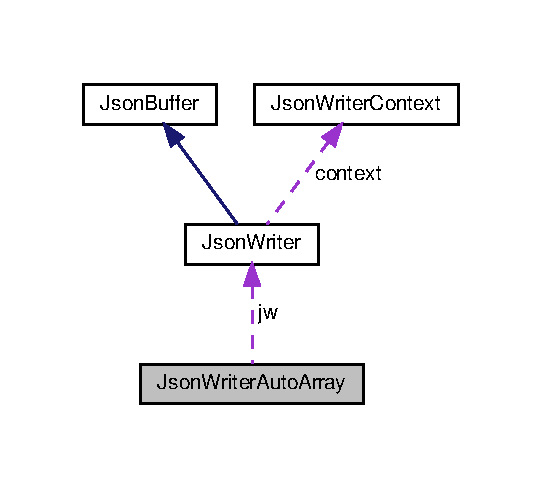
\includegraphics[width=260pt]{class_json_writer_auto_array__coll__graph}
\end{center}
\end{figure}
\subsection*{Public Member Functions}
\begin{DoxyCompactItemize}
\item 
\hyperlink{class_json_writer_auto_array_a6bfd8fc01e5bcdd38cbf4b1c2e91637b}{Json\+Writer\+Auto\+Array} (\hyperlink{class_json_writer}{Json\+Writer} $\ast$\hyperlink{class_json_writer_auto_array_a747001de80facbc7a782a9e14ad2acae}{jw})
\begin{DoxyCompactList}\small\item\em Start a new array. \end{DoxyCompactList}\item 
\hyperlink{class_json_writer_auto_array_a2554fc87e46846becf528e878d043bc0}{$\sim$\+Json\+Writer\+Auto\+Array} ()
\begin{DoxyCompactList}\small\item\em End the array. \end{DoxyCompactList}\end{DoxyCompactItemize}
\subsection*{Protected Attributes}
\begin{DoxyCompactItemize}
\item 
\hyperlink{class_json_writer}{Json\+Writer} $\ast$ \hyperlink{class_json_writer_auto_array_a747001de80facbc7a782a9e14ad2acae}{jw}
\begin{DoxyCompactList}\small\item\em \hyperlink{class_json_writer}{Json\+Writer} to write to. \end{DoxyCompactList}\end{DoxyCompactItemize}


\subsection{Detailed Description}
Class for creating a J\+S\+ON array with \hyperlink{class_json_writer}{Json\+Writer}. 

When you create an object, you must call start\+Array() to start and finish\+Object\+Or\+Array() to complete it.

This class is instantiated on the stack to automatically start and finish for you. 

Definition at line 1285 of file Json\+Parser\+Generator\+R\+K.\+h.



\subsection{Constructor \& Destructor Documentation}
\mbox{\Hypertarget{class_json_writer_auto_array_a6bfd8fc01e5bcdd38cbf4b1c2e91637b}\label{class_json_writer_auto_array_a6bfd8fc01e5bcdd38cbf4b1c2e91637b}} 
\index{Json\+Writer\+Auto\+Array@{Json\+Writer\+Auto\+Array}!Json\+Writer\+Auto\+Array@{Json\+Writer\+Auto\+Array}}
\index{Json\+Writer\+Auto\+Array@{Json\+Writer\+Auto\+Array}!Json\+Writer\+Auto\+Array@{Json\+Writer\+Auto\+Array}}
\subsubsection{\texorpdfstring{Json\+Writer\+Auto\+Array()}{JsonWriterAutoArray()}}
{\footnotesize\ttfamily Json\+Writer\+Auto\+Array\+::\+Json\+Writer\+Auto\+Array (\begin{DoxyParamCaption}\item[{\hyperlink{class_json_writer}{Json\+Writer} $\ast$}]{jw }\end{DoxyParamCaption})\hspace{0.3cm}{\ttfamily [inline]}}



Start a new array. 


\begin{DoxyParams}{Parameters}
{\em jw} & The \hyperlink{class_json_writer}{Json\+Writer} object to insert the array into \\
\hline
\end{DoxyParams}


Definition at line 1292 of file Json\+Parser\+Generator\+R\+K.\+h.



References jw, and Json\+Writer\+::start\+Array().

\mbox{\Hypertarget{class_json_writer_auto_array_a2554fc87e46846becf528e878d043bc0}\label{class_json_writer_auto_array_a2554fc87e46846becf528e878d043bc0}} 
\index{Json\+Writer\+Auto\+Array@{Json\+Writer\+Auto\+Array}!````~Json\+Writer\+Auto\+Array@{$\sim$\+Json\+Writer\+Auto\+Array}}
\index{````~Json\+Writer\+Auto\+Array@{$\sim$\+Json\+Writer\+Auto\+Array}!Json\+Writer\+Auto\+Array@{Json\+Writer\+Auto\+Array}}
\subsubsection{\texorpdfstring{$\sim$\+Json\+Writer\+Auto\+Array()}{~JsonWriterAutoArray()}}
{\footnotesize\ttfamily Json\+Writer\+Auto\+Array\+::$\sim$\+Json\+Writer\+Auto\+Array (\begin{DoxyParamCaption}{ }\end{DoxyParamCaption})\hspace{0.3cm}{\ttfamily [inline]}}



End the array. 



Definition at line 1299 of file Json\+Parser\+Generator\+R\+K.\+h.



References Json\+Writer\+::finish\+Object\+Or\+Array(), and jw.



\subsection{Member Data Documentation}
\mbox{\Hypertarget{class_json_writer_auto_array_a747001de80facbc7a782a9e14ad2acae}\label{class_json_writer_auto_array_a747001de80facbc7a782a9e14ad2acae}} 
\index{Json\+Writer\+Auto\+Array@{Json\+Writer\+Auto\+Array}!jw@{jw}}
\index{jw@{jw}!Json\+Writer\+Auto\+Array@{Json\+Writer\+Auto\+Array}}
\subsubsection{\texorpdfstring{jw}{jw}}
{\footnotesize\ttfamily \hyperlink{class_json_writer}{Json\+Writer}$\ast$ Json\+Writer\+Auto\+Array\+::jw\hspace{0.3cm}{\ttfamily [protected]}}



\hyperlink{class_json_writer}{Json\+Writer} to write to. 



Definition at line 1304 of file Json\+Parser\+Generator\+R\+K.\+h.



Referenced by Json\+Writer\+Auto\+Array(), and $\sim$\+Json\+Writer\+Auto\+Array().



The documentation for this class was generated from the following file\+:\begin{DoxyCompactItemize}
\item 
lib/\+Json\+Parser\+Generator\+R\+K/src/\hyperlink{_json_parser_generator_r_k_8h}{Json\+Parser\+Generator\+R\+K.\+h}\end{DoxyCompactItemize}

\hypertarget{class_json_writer_auto_object}{}\section{Json\+Writer\+Auto\+Object Class Reference}
\label{class_json_writer_auto_object}\index{Json\+Writer\+Auto\+Object@{Json\+Writer\+Auto\+Object}}


Class for creating a J\+S\+ON object with \hyperlink{class_json_writer}{Json\+Writer}.  




{\ttfamily \#include $<$Json\+Parser\+Generator\+R\+K.\+h$>$}



Collaboration diagram for Json\+Writer\+Auto\+Object\+:\nopagebreak
\begin{figure}[H]
\begin{center}
\leavevmode
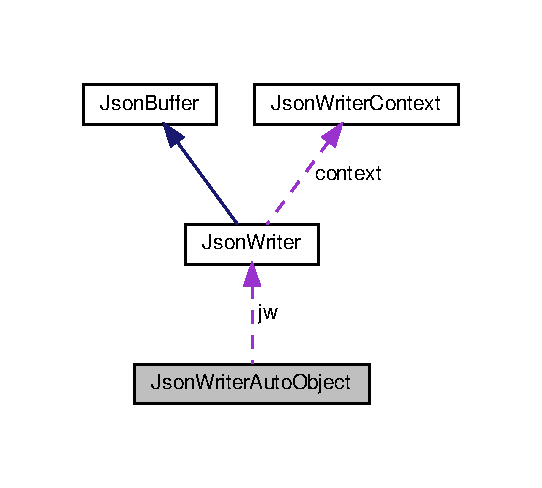
\includegraphics[width=260pt]{class_json_writer_auto_object__coll__graph}
\end{center}
\end{figure}
\subsection*{Public Member Functions}
\begin{DoxyCompactItemize}
\item 
\hyperlink{class_json_writer_auto_object_a92e7cbe4161ff0bd184791e1d666e95f}{Json\+Writer\+Auto\+Object} (\hyperlink{class_json_writer}{Json\+Writer} $\ast$\hyperlink{class_json_writer_auto_object_a4ffea7af57b2ceb87edd5e7ee08aeefb}{jw})
\begin{DoxyCompactList}\small\item\em Start a new object. \end{DoxyCompactList}\item 
\hyperlink{class_json_writer_auto_object_adb79acd280cd69ae5d0d6afea1c187bc}{$\sim$\+Json\+Writer\+Auto\+Object} ()
\begin{DoxyCompactList}\small\item\em End the object. \end{DoxyCompactList}\end{DoxyCompactItemize}
\subsection*{Protected Attributes}
\begin{DoxyCompactItemize}
\item 
\hyperlink{class_json_writer}{Json\+Writer} $\ast$ \hyperlink{class_json_writer_auto_object_a4ffea7af57b2ceb87edd5e7ee08aeefb}{jw}
\begin{DoxyCompactList}\small\item\em \hyperlink{class_json_writer}{Json\+Writer} to write to. \end{DoxyCompactList}\end{DoxyCompactItemize}


\subsection{Detailed Description}
Class for creating a J\+S\+ON object with \hyperlink{class_json_writer}{Json\+Writer}. 

When you create an object, you must call start\+Object() to start and finish\+Object\+Or\+Array() to complete it.

This class is instantiated on the stack to automatically start and finish for you. 

Definition at line 1256 of file Json\+Parser\+Generator\+R\+K.\+h.



\subsection{Constructor \& Destructor Documentation}
\mbox{\Hypertarget{class_json_writer_auto_object_a92e7cbe4161ff0bd184791e1d666e95f}\label{class_json_writer_auto_object_a92e7cbe4161ff0bd184791e1d666e95f}} 
\index{Json\+Writer\+Auto\+Object@{Json\+Writer\+Auto\+Object}!Json\+Writer\+Auto\+Object@{Json\+Writer\+Auto\+Object}}
\index{Json\+Writer\+Auto\+Object@{Json\+Writer\+Auto\+Object}!Json\+Writer\+Auto\+Object@{Json\+Writer\+Auto\+Object}}
\subsubsection{\texorpdfstring{Json\+Writer\+Auto\+Object()}{JsonWriterAutoObject()}}
{\footnotesize\ttfamily Json\+Writer\+Auto\+Object\+::\+Json\+Writer\+Auto\+Object (\begin{DoxyParamCaption}\item[{\hyperlink{class_json_writer}{Json\+Writer} $\ast$}]{jw }\end{DoxyParamCaption})\hspace{0.3cm}{\ttfamily [inline]}}



Start a new object. 


\begin{DoxyParams}{Parameters}
{\em jw} & The \hyperlink{class_json_writer}{Json\+Writer} object to insert the object into \\
\hline
\end{DoxyParams}


Definition at line 1263 of file Json\+Parser\+Generator\+R\+K.\+h.



References jw, and Json\+Writer\+::start\+Object().



Referenced by run\+Test().

\mbox{\Hypertarget{class_json_writer_auto_object_adb79acd280cd69ae5d0d6afea1c187bc}\label{class_json_writer_auto_object_adb79acd280cd69ae5d0d6afea1c187bc}} 
\index{Json\+Writer\+Auto\+Object@{Json\+Writer\+Auto\+Object}!````~Json\+Writer\+Auto\+Object@{$\sim$\+Json\+Writer\+Auto\+Object}}
\index{````~Json\+Writer\+Auto\+Object@{$\sim$\+Json\+Writer\+Auto\+Object}!Json\+Writer\+Auto\+Object@{Json\+Writer\+Auto\+Object}}
\subsubsection{\texorpdfstring{$\sim$\+Json\+Writer\+Auto\+Object()}{~JsonWriterAutoObject()}}
{\footnotesize\ttfamily Json\+Writer\+Auto\+Object\+::$\sim$\+Json\+Writer\+Auto\+Object (\begin{DoxyParamCaption}{ }\end{DoxyParamCaption})\hspace{0.3cm}{\ttfamily [inline]}}



End the object. 



Definition at line 1270 of file Json\+Parser\+Generator\+R\+K.\+h.



References Json\+Writer\+::finish\+Object\+Or\+Array(), and jw.



\subsection{Member Data Documentation}
\mbox{\Hypertarget{class_json_writer_auto_object_a4ffea7af57b2ceb87edd5e7ee08aeefb}\label{class_json_writer_auto_object_a4ffea7af57b2ceb87edd5e7ee08aeefb}} 
\index{Json\+Writer\+Auto\+Object@{Json\+Writer\+Auto\+Object}!jw@{jw}}
\index{jw@{jw}!Json\+Writer\+Auto\+Object@{Json\+Writer\+Auto\+Object}}
\subsubsection{\texorpdfstring{jw}{jw}}
{\footnotesize\ttfamily \hyperlink{class_json_writer}{Json\+Writer}$\ast$ Json\+Writer\+Auto\+Object\+::jw\hspace{0.3cm}{\ttfamily [protected]}}



\hyperlink{class_json_writer}{Json\+Writer} to write to. 



Definition at line 1275 of file Json\+Parser\+Generator\+R\+K.\+h.



Referenced by Json\+Writer\+Auto\+Object(), and $\sim$\+Json\+Writer\+Auto\+Object().



The documentation for this class was generated from the following file\+:\begin{DoxyCompactItemize}
\item 
lib/\+Json\+Parser\+Generator\+R\+K/src/\hyperlink{_json_parser_generator_r_k_8h}{Json\+Parser\+Generator\+R\+K.\+h}\end{DoxyCompactItemize}

\hypertarget{struct_json_writer_context}{}\section{Json\+Writer\+Context Struct Reference}
\label{struct_json_writer_context}\index{Json\+Writer\+Context@{Json\+Writer\+Context}}


Used internally by \hyperlink{class_json_writer}{Json\+Writer}.  




{\ttfamily \#include $<$Json\+Parser\+Generator\+R\+K.\+h$>$}

\subsection*{Public Attributes}
\begin{DoxyCompactItemize}
\item 
bool \hyperlink{struct_json_writer_context_a533afb7eeecfe191549f1db1f596633d}{is\+First}
\begin{DoxyCompactList}\small\item\em True if this the first element in this object or array and doesn\textquotesingle{}t need a comma before it. \end{DoxyCompactList}\item 
char \hyperlink{struct_json_writer_context_ae37822121661863a0d70776b48cc3962}{terminator}
\begin{DoxyCompactList}\small\item\em The character that will terminate the object or array when ended. \end{DoxyCompactList}\end{DoxyCompactItemize}


\subsection{Detailed Description}
Used internally by \hyperlink{class_json_writer}{Json\+Writer}. 

Definition at line 902 of file Json\+Parser\+Generator\+R\+K.\+h.



\subsection{Member Data Documentation}
\mbox{\Hypertarget{struct_json_writer_context_a533afb7eeecfe191549f1db1f596633d}\label{struct_json_writer_context_a533afb7eeecfe191549f1db1f596633d}} 
\index{Json\+Writer\+Context@{Json\+Writer\+Context}!is\+First@{is\+First}}
\index{is\+First@{is\+First}!Json\+Writer\+Context@{Json\+Writer\+Context}}
\subsubsection{\texorpdfstring{is\+First}{isFirst}}
{\footnotesize\ttfamily bool Json\+Writer\+Context\+::is\+First}



True if this the first element in this object or array and doesn\textquotesingle{}t need a comma before it. 



Definition at line 903 of file Json\+Parser\+Generator\+R\+K.\+h.



Referenced by Json\+Writer\+::init(), Json\+Writer\+::insert\+Check\+Separator(), Json\+Writer\+::set\+Is\+First(), and Json\+Writer\+::start\+Object\+Or\+Array().

\mbox{\Hypertarget{struct_json_writer_context_ae37822121661863a0d70776b48cc3962}\label{struct_json_writer_context_ae37822121661863a0d70776b48cc3962}} 
\index{Json\+Writer\+Context@{Json\+Writer\+Context}!terminator@{terminator}}
\index{terminator@{terminator}!Json\+Writer\+Context@{Json\+Writer\+Context}}
\subsubsection{\texorpdfstring{terminator}{terminator}}
{\footnotesize\ttfamily char Json\+Writer\+Context\+::terminator}



The character that will terminate the object or array when ended. 



Definition at line 904 of file Json\+Parser\+Generator\+R\+K.\+h.



Referenced by Json\+Writer\+::finish\+Object\+Or\+Array(), Json\+Writer\+::init(), and Json\+Writer\+::start\+Object\+Or\+Array().



The documentation for this struct was generated from the following file\+:\begin{DoxyCompactItemize}
\item 
lib/\+Json\+Parser\+Generator\+R\+K/src/\hyperlink{_json_parser_generator_r_k_8h}{Json\+Parser\+Generator\+R\+K.\+h}\end{DoxyCompactItemize}

\section{Json\+Writer\+Static$<$ B\+U\+F\+F\+E\+R\+\_\+\+S\+I\+ZE $>$ Class Template Reference}
\label{class_json_writer_static}\index{Json\+Writer\+Static$<$ B\+U\+F\+F\+E\+R\+\_\+\+S\+I\+Z\+E $>$@{Json\+Writer\+Static$<$ B\+U\+F\+F\+E\+R\+\_\+\+S\+I\+Z\+E $>$}}


Creates a \doxyref{Json\+Writer}{p.}{class_json_writer} with a statically allocated buffer.  




{\ttfamily \#include $<$Json\+Parser\+Generator\+R\+K.\+h$>$}



Inheritance diagram for Json\+Writer\+Static$<$ B\+U\+F\+F\+E\+R\+\_\+\+S\+I\+ZE $>$\+:\nopagebreak
\begin{figure}[H]
\begin{center}
\leavevmode
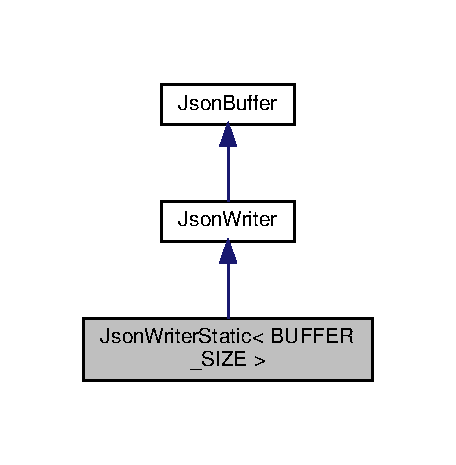
\includegraphics[width=219pt]{class_json_writer_static__inherit__graph}
\end{center}
\end{figure}


Collaboration diagram for Json\+Writer\+Static$<$ B\+U\+F\+F\+E\+R\+\_\+\+S\+I\+ZE $>$\+:\nopagebreak
\begin{figure}[H]
\begin{center}
\leavevmode
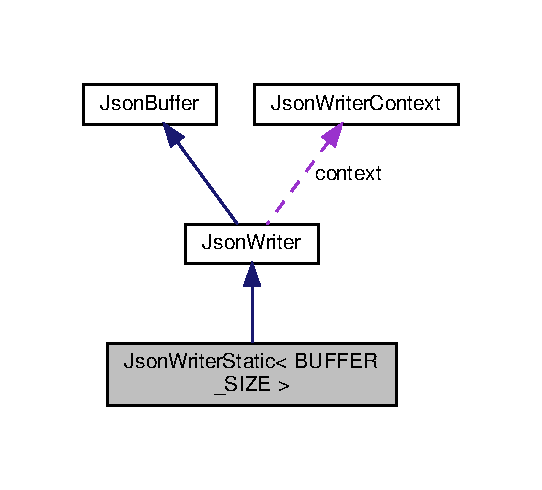
\includegraphics[width=260pt]{class_json_writer_static__coll__graph}
\end{center}
\end{figure}
\subsection*{Public Member Functions}
\begin{DoxyCompactItemize}
\item 
\textbf{ Json\+Writer\+Static} ()
\end{DoxyCompactItemize}
\subsection*{Private Attributes}
\begin{DoxyCompactItemize}
\item 
char \textbf{ static\+Buffer} [B\+U\+F\+F\+E\+R\+\_\+\+S\+I\+ZE]
\begin{DoxyCompactList}\small\item\em static buffer to write to \end{DoxyCompactList}\end{DoxyCompactItemize}
\subsection*{Additional Inherited Members}


\subsection{Detailed Description}
\subsubsection*{template$<$size\+\_\+t B\+U\+F\+F\+E\+R\+\_\+\+S\+I\+ZE$>$\newline
class Json\+Writer\+Static$<$ B\+U\+F\+F\+E\+R\+\_\+\+S\+I\+Z\+E $>$}

Creates a \doxyref{Json\+Writer}{p.}{class_json_writer} with a statically allocated buffer. 

You typically do this when you want to create a buffer as a global variable.

Example\+:


\begin{DoxyCode}
JsonWriterStatic<256> jsonWriter;
\end{DoxyCode}


Creates a 256 byte buffer to write J\+S\+ON to. You\textquotesingle{}d normally do this as a global variable, but for smaller buffers (256 and smaller should be fine) in the loop thread, you can allocate one on the stack as a local variable.


\begin{DoxyParams}{Parameters}
{\em B\+U\+F\+F\+E\+R\+\_\+\+S\+I\+ZE} & The size of the buffer to reserve. \\
\hline
\end{DoxyParams}


Definition at line 1241 of file Json\+Parser\+Generator\+R\+K.\+h.



\subsection{Constructor \& Destructor Documentation}
\mbox{\label{class_json_writer_static_aef07dcd39c03c2f34566c84a3408f922}} 
\index{Json\+Writer\+Static@{Json\+Writer\+Static}!Json\+Writer\+Static@{Json\+Writer\+Static}}
\index{Json\+Writer\+Static@{Json\+Writer\+Static}!Json\+Writer\+Static@{Json\+Writer\+Static}}
\subsubsection{Json\+Writer\+Static()}
{\footnotesize\ttfamily template$<$size\+\_\+t B\+U\+F\+F\+E\+R\+\_\+\+S\+I\+ZE$>$ \\
\textbf{ Json\+Writer\+Static}$<$ B\+U\+F\+F\+E\+R\+\_\+\+S\+I\+ZE $>$\+::\textbf{ Json\+Writer\+Static} (\begin{DoxyParamCaption}{ }\end{DoxyParamCaption})\hspace{0.3cm}{\ttfamily [inline]}, {\ttfamily [explicit]}}



Definition at line 1243 of file Json\+Parser\+Generator\+R\+K.\+h.


\begin{DoxyCode}
1243 : JsonWriter(staticBuffer, BUFFER\_SIZE) \{\};
\end{DoxyCode}


\subsection{Member Data Documentation}
\mbox{\label{class_json_writer_static_af733d279f0980f674ce08c15f71cc358}} 
\index{Json\+Writer\+Static@{Json\+Writer\+Static}!static\+Buffer@{static\+Buffer}}
\index{static\+Buffer@{static\+Buffer}!Json\+Writer\+Static@{Json\+Writer\+Static}}
\subsubsection{static\+Buffer}
{\footnotesize\ttfamily template$<$size\+\_\+t B\+U\+F\+F\+E\+R\+\_\+\+S\+I\+ZE$>$ \\
char \textbf{ Json\+Writer\+Static}$<$ B\+U\+F\+F\+E\+R\+\_\+\+S\+I\+ZE $>$\+::static\+Buffer[B\+U\+F\+F\+E\+R\+\_\+\+S\+I\+ZE]\hspace{0.3cm}{\ttfamily [private]}}



static buffer to write to 



Definition at line 1243 of file Json\+Parser\+Generator\+R\+K.\+h.



The documentation for this class was generated from the following file\+:\begin{DoxyCompactItemize}
\item 
lib/\+Json\+Parser\+Generator\+R\+K/src/\textbf{ Json\+Parser\+Generator\+R\+K.\+h}\end{DoxyCompactItemize}

\hypertarget{class_m_f_r_c522}{}\section{M\+F\+R\+C522 Class Reference}
\label{class_m_f_r_c522}\index{M\+F\+R\+C522@{M\+F\+R\+C522}}


{\ttfamily \#include $<$M\+F\+R\+C522.\+h$>$}



Collaboration diagram for M\+F\+R\+C522\+:\nopagebreak
\begin{figure}[H]
\begin{center}
\leavevmode
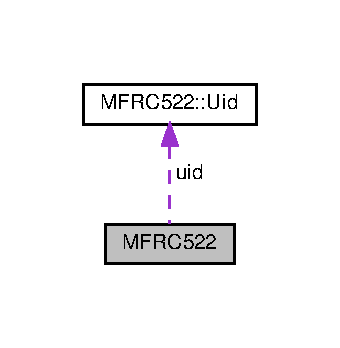
\includegraphics[width=163pt]{class_m_f_r_c522__coll__graph}
\end{center}
\end{figure}
\subsection*{Classes}
\begin{DoxyCompactItemize}
\item 
struct \hyperlink{struct_m_f_r_c522_1_1_m_i_f_a_r_e___key}{M\+I\+F\+A\+R\+E\+\_\+\+Key}
\item 
struct \hyperlink{struct_m_f_r_c522_1_1_uid}{Uid}
\end{DoxyCompactItemize}
\subsection*{Public Types}
\begin{DoxyCompactItemize}
\item 
enum \hyperlink{class_m_f_r_c522_ae3b374c61bf50256289349fdb78fe181}{P\+C\+D\+\_\+\+Register} \{ \newline
\hyperlink{class_m_f_r_c522_ae3b374c61bf50256289349fdb78fe181a0ec37643fa721f476b0cd4359e3c7ef1}{Command\+Reg} = 0x01 $<$$<$ 1, 
\hyperlink{class_m_f_r_c522_ae3b374c61bf50256289349fdb78fe181ad956725472615518dfb99f2d7dccc50e}{Com\+I\+En\+Reg} = 0x02 $<$$<$ 1, 
\hyperlink{class_m_f_r_c522_ae3b374c61bf50256289349fdb78fe181afb4527cc3e364cce3fe3e62cdcde7da0}{Div\+I\+En\+Reg} = 0x03 $<$$<$ 1, 
\hyperlink{class_m_f_r_c522_ae3b374c61bf50256289349fdb78fe181a76b2a615444982e04566784bdb5c9841}{Com\+Irq\+Reg} = 0x04 $<$$<$ 1, 
\newline
\hyperlink{class_m_f_r_c522_ae3b374c61bf50256289349fdb78fe181a95e26d5ece97ae43c34d08797205a356}{Div\+Irq\+Reg} = 0x05 $<$$<$ 1, 
\hyperlink{class_m_f_r_c522_ae3b374c61bf50256289349fdb78fe181a240aa03a1d9542235b89cdef377a5796}{Error\+Reg} = 0x06 $<$$<$ 1, 
\hyperlink{class_m_f_r_c522_ae3b374c61bf50256289349fdb78fe181a9f8b10dda6868e74226ab7ccca8d5be0}{Status1\+Reg} = 0x07 $<$$<$ 1, 
\hyperlink{class_m_f_r_c522_ae3b374c61bf50256289349fdb78fe181a8fb1a8c28b7a860793831566373f172f}{Status2\+Reg} = 0x08 $<$$<$ 1, 
\newline
\hyperlink{class_m_f_r_c522_ae3b374c61bf50256289349fdb78fe181afdbfd2f397b96d1043c808ec26e80328}{F\+I\+F\+O\+Data\+Reg} = 0x09 $<$$<$ 1, 
\hyperlink{class_m_f_r_c522_ae3b374c61bf50256289349fdb78fe181a35e5daf30358a0a271dadf50ba6bb4e7}{F\+I\+F\+O\+Level\+Reg} = 0x0A $<$$<$ 1, 
\hyperlink{class_m_f_r_c522_ae3b374c61bf50256289349fdb78fe181aee5f7c4d0d34d93e5ac67a47e886b224}{Water\+Level\+Reg} = 0x0B $<$$<$ 1, 
\hyperlink{class_m_f_r_c522_ae3b374c61bf50256289349fdb78fe181a9d0df9e03ad6706004b003e20127a76a}{Control\+Reg} = 0x0C $<$$<$ 1, 
\newline
\hyperlink{class_m_f_r_c522_ae3b374c61bf50256289349fdb78fe181aaf8beb5a739cd8bf94b8b5c8d2d109ce}{Bit\+Framing\+Reg} = 0x0D $<$$<$ 1, 
\hyperlink{class_m_f_r_c522_ae3b374c61bf50256289349fdb78fe181afafb7ec88f79c9b1f195195497d0ca07}{Coll\+Reg} = 0x0E $<$$<$ 1, 
\hyperlink{class_m_f_r_c522_ae3b374c61bf50256289349fdb78fe181a2cd647ad1ac1327d2a632115cd9c4477}{Mode\+Reg} = 0x11 $<$$<$ 1, 
\hyperlink{class_m_f_r_c522_ae3b374c61bf50256289349fdb78fe181ad4fe18ad01abc83d4559369226fe7992}{Tx\+Mode\+Reg} = 0x12 $<$$<$ 1, 
\newline
\hyperlink{class_m_f_r_c522_ae3b374c61bf50256289349fdb78fe181a7e0d6ae1fdd25be6d80d1b76b2274764}{Rx\+Mode\+Reg} = 0x13 $<$$<$ 1, 
\hyperlink{class_m_f_r_c522_ae3b374c61bf50256289349fdb78fe181a73dc12b03f05177a400263e5e2bcf0cc}{Tx\+Control\+Reg} = 0x14 $<$$<$ 1, 
\hyperlink{class_m_f_r_c522_ae3b374c61bf50256289349fdb78fe181ac9de33ca066ca9481bd01d5642a0c879}{Tx\+A\+S\+K\+Reg} = 0x15 $<$$<$ 1, 
\hyperlink{class_m_f_r_c522_ae3b374c61bf50256289349fdb78fe181a6cf11e077148648aaec0492317be5177}{Tx\+Sel\+Reg} = 0x16 $<$$<$ 1, 
\newline
\hyperlink{class_m_f_r_c522_ae3b374c61bf50256289349fdb78fe181a669c0c9418d5437566b4b42da326c05f}{Rx\+Sel\+Reg} = 0x17 $<$$<$ 1, 
\hyperlink{class_m_f_r_c522_ae3b374c61bf50256289349fdb78fe181a50d7af7ddc6c606c2b3b9c07df2f22ab}{Rx\+Threshold\+Reg} = 0x18 $<$$<$ 1, 
\hyperlink{class_m_f_r_c522_ae3b374c61bf50256289349fdb78fe181a37b01e93fff19ca62364e8f4f797a5c4}{Demod\+Reg} = 0x19 $<$$<$ 1, 
\hyperlink{class_m_f_r_c522_ae3b374c61bf50256289349fdb78fe181a08eb51f4d08a41ceb4b34189bb712dc7}{Mf\+Tx\+Reg} = 0x1C $<$$<$ 1, 
\newline
\hyperlink{class_m_f_r_c522_ae3b374c61bf50256289349fdb78fe181a92fbf63612de021d242465d4685f1754}{Mf\+Rx\+Reg} = 0x1D $<$$<$ 1, 
\hyperlink{class_m_f_r_c522_ae3b374c61bf50256289349fdb78fe181a23529258de3c3f5655afa2849f547f68}{Serial\+Speed\+Reg} = 0x1F $<$$<$ 1, 
\hyperlink{class_m_f_r_c522_ae3b374c61bf50256289349fdb78fe181a430d34a355d45528d674ad839a187494}{C\+R\+C\+Result\+RegH} = 0x21 $<$$<$ 1, 
\hyperlink{class_m_f_r_c522_ae3b374c61bf50256289349fdb78fe181a4be013336d7bab727dc0e7e150dcd03c}{C\+R\+C\+Result\+RegL} = 0x22 $<$$<$ 1, 
\newline
\hyperlink{class_m_f_r_c522_ae3b374c61bf50256289349fdb78fe181ad69a6a3d883ebfc993fc6fbdbc035508}{Mod\+Width\+Reg} = 0x24 $<$$<$ 1, 
\hyperlink{class_m_f_r_c522_ae3b374c61bf50256289349fdb78fe181a0c99eea491c71e9d2a02bf8a86988adf}{R\+F\+Cfg\+Reg} = 0x26 $<$$<$ 1, 
\hyperlink{class_m_f_r_c522_ae3b374c61bf50256289349fdb78fe181a2f81aa5f433fa51bb4b41cd8955de794}{Gs\+N\+Reg} = 0x27 $<$$<$ 1, 
\hyperlink{class_m_f_r_c522_ae3b374c61bf50256289349fdb78fe181a02925dc7a230fcf039c597bf8cfa113f}{C\+W\+Gs\+P\+Reg} = 0x28 $<$$<$ 1, 
\newline
\hyperlink{class_m_f_r_c522_ae3b374c61bf50256289349fdb78fe181acf6ed89766ba2a4e6483b3209b1aa74e}{Mod\+Gs\+P\+Reg} = 0x29 $<$$<$ 1, 
\hyperlink{class_m_f_r_c522_ae3b374c61bf50256289349fdb78fe181a1ed52e7f88c8bf3fda91bf31bb62afe4}{T\+Mode\+Reg} = 0x2A $<$$<$ 1, 
\hyperlink{class_m_f_r_c522_ae3b374c61bf50256289349fdb78fe181a88c2ad7cdfb7178ea775c157f4ce5213}{T\+Prescaler\+Reg} = 0x2B $<$$<$ 1, 
\hyperlink{class_m_f_r_c522_ae3b374c61bf50256289349fdb78fe181ac9a037a517ada62924c47d5e4b62a14c}{T\+Reload\+RegH} = 0x2C $<$$<$ 1, 
\newline
\hyperlink{class_m_f_r_c522_ae3b374c61bf50256289349fdb78fe181afa3348d82b026de8fecdd18d58e92e2a}{T\+Reload\+RegL} = 0x2D $<$$<$ 1, 
\hyperlink{class_m_f_r_c522_ae3b374c61bf50256289349fdb78fe181ab32cff60c4488866726d4a3930ad8995}{T\+Counter\+Value\+RegH} = 0x2E $<$$<$ 1, 
\hyperlink{class_m_f_r_c522_ae3b374c61bf50256289349fdb78fe181ad70c519d4928690a1d8e7835532ce146}{T\+Counter\+Value\+RegL} = 0x2F $<$$<$ 1, 
\hyperlink{class_m_f_r_c522_ae3b374c61bf50256289349fdb78fe181a3fd81beec1ed6566ff1897aac235890f}{Test\+Sel1\+Reg} = 0x31 $<$$<$ 1, 
\newline
\hyperlink{class_m_f_r_c522_ae3b374c61bf50256289349fdb78fe181ac1053bcb64682eba4a767caaea677807}{Test\+Sel2\+Reg} = 0x32 $<$$<$ 1, 
\hyperlink{class_m_f_r_c522_ae3b374c61bf50256289349fdb78fe181a62a7871c0d3452a8f642bbea0ca7cb34}{Test\+Pin\+En\+Reg} = 0x33 $<$$<$ 1, 
\hyperlink{class_m_f_r_c522_ae3b374c61bf50256289349fdb78fe181aa5bb4445abb525ddf46c6efcb21e8811}{Test\+Pin\+Value\+Reg} = 0x34 $<$$<$ 1, 
\hyperlink{class_m_f_r_c522_ae3b374c61bf50256289349fdb78fe181a37bc0188996dc1ee5332d40961bffb4b}{Test\+Bus\+Reg} = 0x35 $<$$<$ 1, 
\newline
\hyperlink{class_m_f_r_c522_ae3b374c61bf50256289349fdb78fe181a9583618ad17a8a20b7a735c7677c8e56}{Auto\+Test\+Reg} = 0x36 $<$$<$ 1, 
\hyperlink{class_m_f_r_c522_ae3b374c61bf50256289349fdb78fe181a4281c25cf6743163ed2e2f903cf17ba9}{Version\+Reg} = 0x37 $<$$<$ 1, 
\hyperlink{class_m_f_r_c522_ae3b374c61bf50256289349fdb78fe181af1d5966b064c10a672e0064d3ccc55c3}{Analog\+Test\+Reg} = 0x38 $<$$<$ 1, 
\hyperlink{class_m_f_r_c522_ae3b374c61bf50256289349fdb78fe181a25334abb5ff680a530e95e6fb0e48a5b}{Test\+D\+A\+C1\+Reg} = 0x39 $<$$<$ 1, 
\newline
\hyperlink{class_m_f_r_c522_ae3b374c61bf50256289349fdb78fe181a505b75aac860302b2959da7fe607e5eb}{Test\+D\+A\+C2\+Reg} = 0x3A $<$$<$ 1, 
\hyperlink{class_m_f_r_c522_ae3b374c61bf50256289349fdb78fe181a1042587aeb71f82f884975ca54c8854a}{Test\+A\+D\+C\+Reg} = 0x3B $<$$<$ 1
 \}
\item 
enum \hyperlink{class_m_f_r_c522_a973011639bbee6ad7035ae4dd49e2e07}{P\+C\+D\+\_\+\+Command} \{ \newline
\hyperlink{class_m_f_r_c522_a973011639bbee6ad7035ae4dd49e2e07afe5ffdce88fe7544cbc49f8947df9ad9}{P\+C\+D\+\_\+\+Idle} = 0x00, 
\hyperlink{class_m_f_r_c522_a973011639bbee6ad7035ae4dd49e2e07a2f3a9f820c74cb11fabdc00e20c7e2fe}{P\+C\+D\+\_\+\+Mem} = 0x01, 
\hyperlink{class_m_f_r_c522_a973011639bbee6ad7035ae4dd49e2e07a3b9535f3e1eb589c05ca9f22f380647a}{P\+C\+D\+\_\+\+Generate\+Random\+ID} = 0x02, 
\hyperlink{class_m_f_r_c522_a973011639bbee6ad7035ae4dd49e2e07a61d1786d5518a1ad71aac8413941f0ac}{P\+C\+D\+\_\+\+Calc\+C\+RC} = 0x03, 
\newline
\hyperlink{class_m_f_r_c522_a973011639bbee6ad7035ae4dd49e2e07af91e3fb8471c0953d69b83b1baf55ae1}{P\+C\+D\+\_\+\+Transmit} = 0x04, 
\hyperlink{class_m_f_r_c522_a973011639bbee6ad7035ae4dd49e2e07a2d0df8c6384dd59ad6276510b4fe992d}{P\+C\+D\+\_\+\+No\+Cmd\+Change} = 0x07, 
\hyperlink{class_m_f_r_c522_a973011639bbee6ad7035ae4dd49e2e07a2ec760e26c27fff63bebee7e9cf844e7}{P\+C\+D\+\_\+\+Receive} = 0x08, 
\hyperlink{class_m_f_r_c522_a973011639bbee6ad7035ae4dd49e2e07af0b7178e7638038db6f8e7016892fafd}{P\+C\+D\+\_\+\+Transceive} = 0x0C, 
\newline
\hyperlink{class_m_f_r_c522_a973011639bbee6ad7035ae4dd49e2e07a903753278eed75d5d1af2390649ec0c2}{P\+C\+D\+\_\+\+M\+F\+Authent} = 0x0E, 
\hyperlink{class_m_f_r_c522_a973011639bbee6ad7035ae4dd49e2e07a8f54a569867f812163c6a9bc3461d03a}{P\+C\+D\+\_\+\+Soft\+Reset} = 0x0F
 \}
\item 
enum \hyperlink{class_m_f_r_c522_ab7e2bdb063a8ab5f8f29bd05e6867335}{P\+C\+D\+\_\+\+Rx\+Gain} \{ \newline
\hyperlink{class_m_f_r_c522_ab7e2bdb063a8ab5f8f29bd05e6867335a4d5e7f6b74ce3912ffdf3305ea263497}{Rx\+Gain\+\_\+18dB} = 0x00 $<$$<$ 4, 
\hyperlink{class_m_f_r_c522_ab7e2bdb063a8ab5f8f29bd05e6867335aab1ac5ba97a5e07ff487f1996352a8e6}{Rx\+Gain\+\_\+23dB} = 0x01 $<$$<$ 4, 
\hyperlink{class_m_f_r_c522_ab7e2bdb063a8ab5f8f29bd05e6867335ac918bee80fae5c763094684ae08bff82}{Rx\+Gain\+\_\+18d\+B\+\_\+2} = 0x02 $<$$<$ 4, 
\hyperlink{class_m_f_r_c522_ab7e2bdb063a8ab5f8f29bd05e6867335ac3b5b39560b326ac91971a41ad167c15}{Rx\+Gain\+\_\+23d\+B\+\_\+2} = 0x03 $<$$<$ 4, 
\newline
\hyperlink{class_m_f_r_c522_ab7e2bdb063a8ab5f8f29bd05e6867335a721f1c7082ea232324d8660844996158}{Rx\+Gain\+\_\+33dB} = 0x04 $<$$<$ 4, 
\hyperlink{class_m_f_r_c522_ab7e2bdb063a8ab5f8f29bd05e6867335af2f57fe1d71de1d17204933084649368}{Rx\+Gain\+\_\+38dB} = 0x05 $<$$<$ 4, 
\hyperlink{class_m_f_r_c522_ab7e2bdb063a8ab5f8f29bd05e6867335abc9602260b5733a23e0be7e0c03b1ec9}{Rx\+Gain\+\_\+43dB} = 0x06 $<$$<$ 4, 
\hyperlink{class_m_f_r_c522_ab7e2bdb063a8ab5f8f29bd05e6867335a13227ab5e3143489b0888671d284301b}{Rx\+Gain\+\_\+48dB} = 0x07 $<$$<$ 4, 
\newline
\hyperlink{class_m_f_r_c522_ab7e2bdb063a8ab5f8f29bd05e6867335a97ffca230ea898a78b5734ae0dd44506}{Rx\+Gain\+\_\+min} = 0x00 $<$$<$ 4, 
\hyperlink{class_m_f_r_c522_ab7e2bdb063a8ab5f8f29bd05e6867335a2b5b3bd5efdc06adc7c5e190919f5568}{Rx\+Gain\+\_\+avg} = 0x04 $<$$<$ 4, 
\hyperlink{class_m_f_r_c522_ab7e2bdb063a8ab5f8f29bd05e6867335a3c59e553655b4e44c10d7deef54576a0}{Rx\+Gain\+\_\+max} = 0x07 $<$$<$ 4
 \}
\item 
enum \hyperlink{class_m_f_r_c522_a5d46a0e2b34b21f51f40ea95795b5e49}{P\+I\+C\+C\+\_\+\+Command} \{ \newline
\hyperlink{class_m_f_r_c522_a5d46a0e2b34b21f51f40ea95795b5e49aee3203a0a40028d3059861464198b688}{P\+I\+C\+C\+\_\+\+C\+M\+D\+\_\+\+R\+E\+QA} = 0x26, 
\hyperlink{class_m_f_r_c522_a5d46a0e2b34b21f51f40ea95795b5e49a9b8fbd1c87d0a6bbe2ef78d192001b3a}{P\+I\+C\+C\+\_\+\+C\+M\+D\+\_\+\+W\+U\+PA} = 0x52, 
\hyperlink{class_m_f_r_c522_a5d46a0e2b34b21f51f40ea95795b5e49ac532079d67a5325cc5b3505cccf6ac8b}{P\+I\+C\+C\+\_\+\+C\+M\+D\+\_\+\+CT} = 0x88, 
\hyperlink{class_m_f_r_c522_a5d46a0e2b34b21f51f40ea95795b5e49aa9329ee8f72f61f5d73bb893b64c08d0}{P\+I\+C\+C\+\_\+\+C\+M\+D\+\_\+\+S\+E\+L\+\_\+\+C\+L1} = 0x93, 
\newline
\hyperlink{class_m_f_r_c522_a5d46a0e2b34b21f51f40ea95795b5e49ab0399cde7122f0bb6dedb584254455c2}{P\+I\+C\+C\+\_\+\+C\+M\+D\+\_\+\+S\+E\+L\+\_\+\+C\+L2} = 0x95, 
\hyperlink{class_m_f_r_c522_a5d46a0e2b34b21f51f40ea95795b5e49a291c265bc0a7b3f303b361582b95cc85}{P\+I\+C\+C\+\_\+\+C\+M\+D\+\_\+\+S\+E\+L\+\_\+\+C\+L3} = 0x97, 
\hyperlink{class_m_f_r_c522_a5d46a0e2b34b21f51f40ea95795b5e49ad1e0cf89f52ca1b503297e59c600ca57}{P\+I\+C\+C\+\_\+\+C\+M\+D\+\_\+\+H\+L\+TA} = 0x50, 
\hyperlink{class_m_f_r_c522_a5d46a0e2b34b21f51f40ea95795b5e49a7ab2b1b2d0f0d668dfb3ac53ec7f08d6}{P\+I\+C\+C\+\_\+\+C\+M\+D\+\_\+\+M\+F\+\_\+\+A\+U\+T\+H\+\_\+\+K\+E\+Y\+\_\+A} = 0x60, 
\newline
\hyperlink{class_m_f_r_c522_a5d46a0e2b34b21f51f40ea95795b5e49a7b37f0b5fd5406b4cebe306608e5be3f}{P\+I\+C\+C\+\_\+\+C\+M\+D\+\_\+\+M\+F\+\_\+\+A\+U\+T\+H\+\_\+\+K\+E\+Y\+\_\+B} = 0x61, 
\hyperlink{class_m_f_r_c522_a5d46a0e2b34b21f51f40ea95795b5e49a2ea95497e35adbc7acbc32c0cb8a574a}{P\+I\+C\+C\+\_\+\+C\+M\+D\+\_\+\+M\+F\+\_\+\+R\+E\+AD} = 0x30, 
\hyperlink{class_m_f_r_c522_a5d46a0e2b34b21f51f40ea95795b5e49a02ccb020ccc6d49d563f0ed1489d8025}{P\+I\+C\+C\+\_\+\+C\+M\+D\+\_\+\+M\+F\+\_\+\+W\+R\+I\+TE} = 0x\+A0, 
\hyperlink{class_m_f_r_c522_a5d46a0e2b34b21f51f40ea95795b5e49a69b2bb1cd2dc0437d6d1fb11eb2796e7}{P\+I\+C\+C\+\_\+\+C\+M\+D\+\_\+\+M\+F\+\_\+\+D\+E\+C\+R\+E\+M\+E\+NT} = 0x\+C0, 
\newline
\hyperlink{class_m_f_r_c522_a5d46a0e2b34b21f51f40ea95795b5e49a454e12c2c815a861a0450d40273f98ef}{P\+I\+C\+C\+\_\+\+C\+M\+D\+\_\+\+M\+F\+\_\+\+I\+N\+C\+R\+E\+M\+E\+NT} = 0x\+C1, 
\hyperlink{class_m_f_r_c522_a5d46a0e2b34b21f51f40ea95795b5e49ab8ed49cb6ed6228acb0c911d60758486}{P\+I\+C\+C\+\_\+\+C\+M\+D\+\_\+\+M\+F\+\_\+\+R\+E\+S\+T\+O\+RE} = 0x\+C2, 
\hyperlink{class_m_f_r_c522_a5d46a0e2b34b21f51f40ea95795b5e49a5d2309094d9fa17125dc90394e5aeaa0}{P\+I\+C\+C\+\_\+\+C\+M\+D\+\_\+\+M\+F\+\_\+\+T\+R\+A\+N\+S\+F\+ER} = 0x\+B0, 
\hyperlink{class_m_f_r_c522_a5d46a0e2b34b21f51f40ea95795b5e49ae8aeabd1ddb73db2f04259c76eaccd8e}{P\+I\+C\+C\+\_\+\+C\+M\+D\+\_\+\+U\+L\+\_\+\+W\+R\+I\+TE} = 0x\+A2
 \}
\item 
enum \hyperlink{class_m_f_r_c522_a92c17a5b83cc4fde3cc3454c03b8eede}{M\+I\+F\+A\+R\+E\+\_\+\+Misc} \{ \hyperlink{class_m_f_r_c522_a92c17a5b83cc4fde3cc3454c03b8eedea3b5fce9bf15481d218872d4584743a1c}{M\+F\+\_\+\+A\+CK} = 0xA, 
\hyperlink{class_m_f_r_c522_a92c17a5b83cc4fde3cc3454c03b8eedea410c51021b253b680b7ec518ccc818ce}{M\+F\+\_\+\+K\+E\+Y\+\_\+\+S\+I\+ZE} = 6
 \}
\item 
enum \hyperlink{class_m_f_r_c522_a3d8d44527557fe596a9ac486d49239de}{P\+I\+C\+C\+\_\+\+Type} \{ \newline
\hyperlink{class_m_f_r_c522_a3d8d44527557fe596a9ac486d49239deaceba425b4eb6fd85de456a04e1ce1565}{P\+I\+C\+C\+\_\+\+T\+Y\+P\+E\+\_\+\+U\+N\+K\+N\+O\+WN} = 0, 
\hyperlink{class_m_f_r_c522_a3d8d44527557fe596a9ac486d49239dea5c8147b0f3970c9db0a177cb44592bc7}{P\+I\+C\+C\+\_\+\+T\+Y\+P\+E\+\_\+\+I\+S\+O\+\_\+14443\+\_\+4} = 1, 
\hyperlink{class_m_f_r_c522_a3d8d44527557fe596a9ac486d49239dea6d211bf0d6e1bed8f7cdb375e9137360}{P\+I\+C\+C\+\_\+\+T\+Y\+P\+E\+\_\+\+I\+S\+O\+\_\+18092} = 2, 
\hyperlink{class_m_f_r_c522_a3d8d44527557fe596a9ac486d49239dea58d34a16ef064d4679cae921ecc4b505}{P\+I\+C\+C\+\_\+\+T\+Y\+P\+E\+\_\+\+M\+I\+F\+A\+R\+E\+\_\+\+M\+I\+NI} = 3, 
\newline
\hyperlink{class_m_f_r_c522_a3d8d44527557fe596a9ac486d49239dea948d034c12fd457923b65f929b1538fb}{P\+I\+C\+C\+\_\+\+T\+Y\+P\+E\+\_\+\+M\+I\+F\+A\+R\+E\+\_\+1K} = 4, 
\hyperlink{class_m_f_r_c522_a3d8d44527557fe596a9ac486d49239dea7d2d0cfef1abe1c457fb72ebcf81fad4}{P\+I\+C\+C\+\_\+\+T\+Y\+P\+E\+\_\+\+M\+I\+F\+A\+R\+E\+\_\+4K} = 5, 
\hyperlink{class_m_f_r_c522_a3d8d44527557fe596a9ac486d49239dea905f84b972470f7d80ed017817ae300c}{P\+I\+C\+C\+\_\+\+T\+Y\+P\+E\+\_\+\+M\+I\+F\+A\+R\+E\+\_\+\+UL} = 6, 
\hyperlink{class_m_f_r_c522_a3d8d44527557fe596a9ac486d49239dea16d53e0355d6214dbe7faf7e37c99002}{P\+I\+C\+C\+\_\+\+T\+Y\+P\+E\+\_\+\+M\+I\+F\+A\+R\+E\+\_\+\+P\+L\+US} = 7, 
\newline
\hyperlink{class_m_f_r_c522_a3d8d44527557fe596a9ac486d49239dea3efaeaa8963b24323f274bab4c1eaf8f}{P\+I\+C\+C\+\_\+\+T\+Y\+P\+E\+\_\+\+T\+N\+P3\+X\+XX} = 8, 
\hyperlink{class_m_f_r_c522_a3d8d44527557fe596a9ac486d49239dea06fbbb7628bd0c595c58b96547cb8960}{P\+I\+C\+C\+\_\+\+T\+Y\+P\+E\+\_\+\+N\+O\+T\+\_\+\+C\+O\+M\+P\+L\+E\+TE} = 255
 \}
\item 
enum \hyperlink{class_m_f_r_c522_ac0da61f475014ccb8c77205287a09c27}{Status\+Code} \{ \newline
\hyperlink{class_m_f_r_c522_ac0da61f475014ccb8c77205287a09c27a3e34ac777020ad63ef7e346dfb813fe7}{S\+T\+A\+T\+U\+S\+\_\+\+OK} = 1, 
\hyperlink{class_m_f_r_c522_ac0da61f475014ccb8c77205287a09c27aa3b0624b83ba5934292d671c73638a54}{S\+T\+A\+T\+U\+S\+\_\+\+E\+R\+R\+OR} = 2, 
\hyperlink{class_m_f_r_c522_ac0da61f475014ccb8c77205287a09c27a2ad63357ec8c38f712ea6fd811056993}{S\+T\+A\+T\+U\+S\+\_\+\+C\+O\+L\+L\+I\+S\+I\+ON} = 3, 
\hyperlink{class_m_f_r_c522_ac0da61f475014ccb8c77205287a09c27a1db4d2ed757f0a638e5018fb994071ae}{S\+T\+A\+T\+U\+S\+\_\+\+T\+I\+M\+E\+O\+UT} = 4, 
\newline
\hyperlink{class_m_f_r_c522_ac0da61f475014ccb8c77205287a09c27a45ce24f67052f4813df3b0f4efaafea8}{S\+T\+A\+T\+U\+S\+\_\+\+N\+O\+\_\+\+R\+O\+OM} = 5, 
\hyperlink{class_m_f_r_c522_ac0da61f475014ccb8c77205287a09c27a851307266f677fd58db61540ffe76855}{S\+T\+A\+T\+U\+S\+\_\+\+I\+N\+T\+E\+R\+N\+A\+L\+\_\+\+E\+R\+R\+OR} = 6, 
\hyperlink{class_m_f_r_c522_ac0da61f475014ccb8c77205287a09c27a88d450f43a9d22ead5db926808599fb5}{S\+T\+A\+T\+U\+S\+\_\+\+I\+N\+V\+A\+L\+ID} = 7, 
\hyperlink{class_m_f_r_c522_ac0da61f475014ccb8c77205287a09c27ac25a91c2efa2dc7638758321374f7566}{S\+T\+A\+T\+U\+S\+\_\+\+C\+R\+C\+\_\+\+W\+R\+O\+NG} = 8, 
\newline
\hyperlink{class_m_f_r_c522_ac0da61f475014ccb8c77205287a09c27ad14f5e1a33047c90b50fa829cb669109}{S\+T\+A\+T\+U\+S\+\_\+\+M\+I\+F\+A\+R\+E\+\_\+\+N\+A\+CK} = 9
 \}
\end{DoxyCompactItemize}
\subsection*{Public Member Functions}
\begin{DoxyCompactItemize}
\item 
\hyperlink{class_m_f_r_c522_a8b859e244e80970594bf333a0148ade1}{M\+F\+R\+C522} (byte chip\+Select\+Pin, byte reset\+Power\+Down\+Pin)
\item 
void \hyperlink{class_m_f_r_c522_a425d73a02db79e17abd78ff805770fc3}{set\+S\+P\+I\+Config} ()
\item 
void \hyperlink{class_m_f_r_c522_aa97f1faf2a4c82b911d7c3ed2535bb59}{P\+C\+D\+\_\+\+Write\+Register} (byte reg, byte value)
\item 
void \hyperlink{class_m_f_r_c522_a2141779996fc50861aafb89f9d12a163}{P\+C\+D\+\_\+\+Write\+Register} (byte reg, byte count, byte $\ast$values)
\item 
byte \hyperlink{class_m_f_r_c522_a4d81572f8b9ed0ffb1f59270cdffc310}{P\+C\+D\+\_\+\+Read\+Register} (byte reg)
\item 
void \hyperlink{class_m_f_r_c522_ad5960b7bc42a9a3ebfa7ccf390ffc356}{P\+C\+D\+\_\+\+Read\+Register} (byte reg, byte count, byte $\ast$values, byte rx\+Align=0)
\item 
void \hyperlink{class_m_f_r_c522_a5b743b53393d88588e9d878159e89faf}{set\+Bit\+Mask} (unsigned char reg, unsigned char mask)
\item 
void \hyperlink{class_m_f_r_c522_adef7552eb0089496522153e7bad19d63}{P\+C\+D\+\_\+\+Set\+Register\+Bit\+Mask} (byte reg, byte mask)
\item 
void \hyperlink{class_m_f_r_c522_a45d4f1b7cdc9eccd9d394d4f5058c503}{P\+C\+D\+\_\+\+Clear\+Register\+Bit\+Mask} (byte reg, byte mask)
\item 
byte \hyperlink{class_m_f_r_c522_a96adb3a83724709c622cc50d5518cbc3}{P\+C\+D\+\_\+\+Calculate\+C\+RC} (byte $\ast$data, byte length, byte $\ast$result)
\item 
void \hyperlink{class_m_f_r_c522_ad681e424fc68a57941bea5702cee05eb}{P\+C\+D\+\_\+\+Init} ()
\item 
void \hyperlink{class_m_f_r_c522_a9886678ea0a65021bf602cfb110caa15}{P\+C\+D\+\_\+\+Reset} ()
\item 
void \hyperlink{class_m_f_r_c522_a044be037a5f172e9cea7d8ce1dcf32e0}{P\+C\+D\+\_\+\+Antenna\+On} ()
\item 
void \hyperlink{class_m_f_r_c522_a2098ebe85700109b20c5026643f1dad7}{P\+C\+D\+\_\+\+Antenna\+Off} ()
\item 
byte \hyperlink{class_m_f_r_c522_aa02ae994a9ebf146475f46fc538cef28}{P\+C\+D\+\_\+\+Get\+Antenna\+Gain} ()
\item 
void \hyperlink{class_m_f_r_c522_a5ce84dd855f2ae297dd00fafaf62ef78}{P\+C\+D\+\_\+\+Set\+Antenna\+Gain} (byte mask)
\item 
byte \hyperlink{class_m_f_r_c522_a4d967509ca687fca2dbfd0d867b38d8d}{P\+C\+D\+\_\+\+Transceive\+Data} (byte $\ast$send\+Data, byte send\+Len, byte $\ast$back\+Data, byte $\ast$back\+Len, byte $\ast$valid\+Bits=N\+U\+LL, byte rx\+Align=0, bool check\+C\+RC=false)
\item 
byte \hyperlink{class_m_f_r_c522_a731cc27ae35b1bba2d2c9d2af28b5c23}{P\+C\+D\+\_\+\+Communicate\+With\+P\+I\+CC} (byte command, byte wait\+I\+Rq, byte $\ast$send\+Data, byte send\+Len, byte $\ast$back\+Data=N\+U\+LL, byte $\ast$back\+Len=N\+U\+LL, byte $\ast$valid\+Bits=N\+U\+LL, byte rx\+Align=0, bool check\+C\+RC=false)
\item 
byte \hyperlink{class_m_f_r_c522_a6db371f6ca95e8ea22445124c79012cc}{P\+I\+C\+C\+\_\+\+RequestA} (byte $\ast$buffer\+A\+T\+QA, byte $\ast$buffer\+Size)
\item 
byte \hyperlink{class_m_f_r_c522_a009dfa9138c6f999af82d7fc5b17a272}{P\+I\+C\+C\+\_\+\+WakeupA} (byte $\ast$buffer\+A\+T\+QA, byte $\ast$buffer\+Size)
\item 
byte \hyperlink{class_m_f_r_c522_a43d475b7d21f31bd1104e81ea5e3d1c9}{P\+I\+C\+C\+\_\+\+R\+E\+Q\+A\+\_\+or\+\_\+\+W\+U\+PA} (byte command, byte $\ast$buffer\+A\+T\+QA, byte $\ast$buffer\+Size)
\item 
byte \hyperlink{class_m_f_r_c522_ab40449ac80501db28d25889612bb2db0}{P\+I\+C\+C\+\_\+\+Select} (\hyperlink{struct_m_f_r_c522_1_1_uid}{Uid} $\ast$\hyperlink{class_m_f_r_c522_ad456545d41962dd7f8bd4210f5618498}{uid}, byte valid\+Bits=0)
\item 
byte \hyperlink{class_m_f_r_c522_aaa152b63193d852bf2edcfae3044bea4}{P\+I\+C\+C\+\_\+\+HaltA} ()
\item 
byte \hyperlink{class_m_f_r_c522_a26469f6295cd9796e0bb781c48036971}{P\+C\+D\+\_\+\+Authenticate} (byte command, byte block\+Addr, \hyperlink{struct_m_f_r_c522_1_1_m_i_f_a_r_e___key}{M\+I\+F\+A\+R\+E\+\_\+\+Key} $\ast$key, \hyperlink{struct_m_f_r_c522_1_1_uid}{Uid} $\ast$\hyperlink{class_m_f_r_c522_ad456545d41962dd7f8bd4210f5618498}{uid})
\item 
void \hyperlink{class_m_f_r_c522_a24d3ab7b2170fdfa3f0121a7256f12d9}{P\+C\+D\+\_\+\+Stop\+Crypto1} ()
\item 
byte \hyperlink{class_m_f_r_c522_a05cdd51aa162e37de1a9439b75901e28}{M\+I\+F\+A\+R\+E\+\_\+\+Read} (byte block\+Addr, byte $\ast$buffer, byte $\ast$buffer\+Size)
\item 
byte \hyperlink{class_m_f_r_c522_a6f3c1ba843a2484314c72daf2e7734f0}{M\+I\+F\+A\+R\+E\+\_\+\+Write} (byte block\+Addr, byte $\ast$buffer, byte buffer\+Size)
\item 
byte \hyperlink{class_m_f_r_c522_a1b4732c54686bd32e2dd79cf4b5279e6}{M\+I\+F\+A\+R\+E\+\_\+\+Decrement} (byte block\+Addr, long delta)
\item 
byte \hyperlink{class_m_f_r_c522_aa45713c6d2c8dcf949874abd03f72327}{M\+I\+F\+A\+R\+E\+\_\+\+Increment} (byte block\+Addr, long delta)
\item 
byte \hyperlink{class_m_f_r_c522_aa0f6201f92ae7babab4d37786a12d483}{M\+I\+F\+A\+R\+E\+\_\+\+Restore} (byte block\+Addr)
\item 
byte \hyperlink{class_m_f_r_c522_a36299391c708a71c11c48a94c4e3f3c2}{M\+I\+F\+A\+R\+E\+\_\+\+Transfer} (byte block\+Addr)
\item 
byte \hyperlink{class_m_f_r_c522_aba2c50d4660897d136cf839940299e07}{M\+I\+F\+A\+R\+E\+\_\+\+Ultralight\+\_\+\+Write} (byte page, byte $\ast$buffer, byte buffer\+Size)
\item 
byte \hyperlink{class_m_f_r_c522_a1116cb31c5a64c2be71e3b8649d7865b}{M\+I\+F\+A\+R\+E\+\_\+\+Get\+Value} (byte block\+Addr, long $\ast$value)
\item 
byte \hyperlink{class_m_f_r_c522_a9ae3cc71bcfb52455349683d3685a919}{M\+I\+F\+A\+R\+E\+\_\+\+Set\+Value} (byte block\+Addr, long value)
\item 
byte \hyperlink{class_m_f_r_c522_a638bcf89cd6356cfbc755004a2e62b1c}{P\+C\+D\+\_\+\+M\+I\+F\+A\+R\+E\+\_\+\+Transceive} (byte $\ast$send\+Data, byte send\+Len, bool accept\+Timeout=false)
\item 
const char $\ast$ \hyperlink{class_m_f_r_c522_a63e898d6efcce838b17778403f7003a9}{Get\+Status\+Code\+Name} (byte code)
\item 
byte \hyperlink{class_m_f_r_c522_a1217f49a195799e3c55b388f9d378ab3}{P\+I\+C\+C\+\_\+\+Get\+Type} (byte sak)
\item 
const char $\ast$ \hyperlink{class_m_f_r_c522_aca99128b3a8a192473d0b715a48b9f97}{P\+I\+C\+C\+\_\+\+Get\+Type\+Name} (byte type)
\item 
void \hyperlink{class_m_f_r_c522_a6f324d43c6fbbd0e260b171747186037}{P\+I\+C\+C\+\_\+\+Dump\+To\+Serial} (\hyperlink{struct_m_f_r_c522_1_1_uid}{Uid} $\ast$\hyperlink{class_m_f_r_c522_ad456545d41962dd7f8bd4210f5618498}{uid})
\item 
void \hyperlink{class_m_f_r_c522_aa45876e611a99b9b6d8ae2d4117d3976}{P\+I\+C\+C\+\_\+\+Dump\+Mifare\+Classic\+To\+Serial} (\hyperlink{struct_m_f_r_c522_1_1_uid}{Uid} $\ast$\hyperlink{class_m_f_r_c522_ad456545d41962dd7f8bd4210f5618498}{uid}, byte picc\+Type, \hyperlink{struct_m_f_r_c522_1_1_m_i_f_a_r_e___key}{M\+I\+F\+A\+R\+E\+\_\+\+Key} $\ast$key)
\item 
void \hyperlink{class_m_f_r_c522_a20c559f09927a7c5f91295f6158e4342}{P\+I\+C\+C\+\_\+\+Dump\+Mifare\+Classic\+Sector\+To\+Serial} (\hyperlink{struct_m_f_r_c522_1_1_uid}{Uid} $\ast$\hyperlink{class_m_f_r_c522_ad456545d41962dd7f8bd4210f5618498}{uid}, \hyperlink{struct_m_f_r_c522_1_1_m_i_f_a_r_e___key}{M\+I\+F\+A\+R\+E\+\_\+\+Key} $\ast$key, byte sector)
\item 
void \hyperlink{class_m_f_r_c522_ac148d28877dd577606a28e9e7e4b6809}{P\+I\+C\+C\+\_\+\+Dump\+Mifare\+Ultralight\+To\+Serial} ()
\item 
void \hyperlink{class_m_f_r_c522_ab8c712963189654e9bc368be8783e2ab}{M\+I\+F\+A\+R\+E\+\_\+\+Set\+Access\+Bits} (byte $\ast$access\+Bit\+Buffer, byte g0, byte g1, byte g2, byte g3)
\item 
bool \hyperlink{class_m_f_r_c522_a925607adc9382720c222578bd236a9c8}{M\+I\+F\+A\+R\+E\+\_\+\+Open\+Uid\+Backdoor} (bool log\+Errors)
\item 
bool \hyperlink{class_m_f_r_c522_a2bdc18af4952ce99099607c84139b51c}{M\+I\+F\+A\+R\+E\+\_\+\+Set\+Uid} (byte $\ast$new\+Uid, byte uid\+Size, bool log\+Errors)
\item 
bool \hyperlink{class_m_f_r_c522_afcbb15d925cb3bea9f58595111fbca48}{M\+I\+F\+A\+R\+E\+\_\+\+Unbrick\+Uid\+Sector} (bool log\+Errors)
\item 
bool \hyperlink{class_m_f_r_c522_a3adca9d3b455c680ebcde3b74c4e567b}{P\+I\+C\+C\+\_\+\+Is\+New\+Card\+Present} ()
\item 
bool \hyperlink{class_m_f_r_c522_aab1218c71cec9cc17ee3ac8a683df106}{P\+I\+C\+C\+\_\+\+Read\+Card\+Serial} ()
\end{DoxyCompactItemize}
\subsection*{Public Attributes}
\begin{DoxyCompactItemize}
\item 
\hyperlink{struct_m_f_r_c522_1_1_uid}{Uid} \hyperlink{class_m_f_r_c522_ad456545d41962dd7f8bd4210f5618498}{uid}
\end{DoxyCompactItemize}
\subsection*{Static Public Attributes}
\begin{DoxyCompactItemize}
\item 
static const byte \hyperlink{class_m_f_r_c522_a7bdf27d2122006aabd423ad71495e5f1}{F\+I\+F\+O\+\_\+\+S\+I\+ZE} = 64
\end{DoxyCompactItemize}
\subsection*{Private Member Functions}
\begin{DoxyCompactItemize}
\item 
byte \hyperlink{class_m_f_r_c522_a539a88f943326b5941aecf06433d9cac}{M\+I\+F\+A\+R\+E\+\_\+\+Two\+Step\+Helper} (byte command, byte block\+Addr, long data)
\end{DoxyCompactItemize}
\subsection*{Private Attributes}
\begin{DoxyCompactItemize}
\item 
byte \hyperlink{class_m_f_r_c522_affaa7030ec6e5984cce845a8ed6df1b2}{\+\_\+chip\+Select\+Pin}
\item 
byte \hyperlink{class_m_f_r_c522_a3885cb4bb582de0045cff2829d59006f}{\+\_\+reset\+Power\+Down\+Pin}
\end{DoxyCompactItemize}


\subsection{Detailed Description}


Definition at line 86 of file M\+F\+R\+C522.\+h.



\subsection{Member Enumeration Documentation}
\mbox{\Hypertarget{class_m_f_r_c522_a92c17a5b83cc4fde3cc3454c03b8eede}\label{class_m_f_r_c522_a92c17a5b83cc4fde3cc3454c03b8eede}} 
\index{M\+F\+R\+C522@{M\+F\+R\+C522}!M\+I\+F\+A\+R\+E\+\_\+\+Misc@{M\+I\+F\+A\+R\+E\+\_\+\+Misc}}
\index{M\+I\+F\+A\+R\+E\+\_\+\+Misc@{M\+I\+F\+A\+R\+E\+\_\+\+Misc}!M\+F\+R\+C522@{M\+F\+R\+C522}}
\subsubsection{\texorpdfstring{M\+I\+F\+A\+R\+E\+\_\+\+Misc}{MIFARE\_Misc}}
{\footnotesize\ttfamily enum \hyperlink{class_m_f_r_c522_a92c17a5b83cc4fde3cc3454c03b8eede}{M\+F\+R\+C522\+::\+M\+I\+F\+A\+R\+E\+\_\+\+Misc}}

\begin{DoxyEnumFields}{Enumerator}
\raisebox{\heightof{T}}[0pt][0pt]{\index{M\+F\+\_\+\+A\+CK@{M\+F\+\_\+\+A\+CK}!M\+F\+R\+C522@{M\+F\+R\+C522}}\index{M\+F\+R\+C522@{M\+F\+R\+C522}!M\+F\+\_\+\+A\+CK@{M\+F\+\_\+\+A\+CK}}}\mbox{\Hypertarget{class_m_f_r_c522_a92c17a5b83cc4fde3cc3454c03b8eedea3b5fce9bf15481d218872d4584743a1c}\label{class_m_f_r_c522_a92c17a5b83cc4fde3cc3454c03b8eedea3b5fce9bf15481d218872d4584743a1c}} 
M\+F\+\_\+\+A\+CK&\\
\hline

\raisebox{\heightof{T}}[0pt][0pt]{\index{M\+F\+\_\+\+K\+E\+Y\+\_\+\+S\+I\+ZE@{M\+F\+\_\+\+K\+E\+Y\+\_\+\+S\+I\+ZE}!M\+F\+R\+C522@{M\+F\+R\+C522}}\index{M\+F\+R\+C522@{M\+F\+R\+C522}!M\+F\+\_\+\+K\+E\+Y\+\_\+\+S\+I\+ZE@{M\+F\+\_\+\+K\+E\+Y\+\_\+\+S\+I\+ZE}}}\mbox{\Hypertarget{class_m_f_r_c522_a92c17a5b83cc4fde3cc3454c03b8eedea410c51021b253b680b7ec518ccc818ce}\label{class_m_f_r_c522_a92c17a5b83cc4fde3cc3454c03b8eedea410c51021b253b680b7ec518ccc818ce}} 
M\+F\+\_\+\+K\+E\+Y\+\_\+\+S\+I\+ZE&\\
\hline

\end{DoxyEnumFields}


Definition at line 221 of file M\+F\+R\+C522.\+h.

\mbox{\Hypertarget{class_m_f_r_c522_a973011639bbee6ad7035ae4dd49e2e07}\label{class_m_f_r_c522_a973011639bbee6ad7035ae4dd49e2e07}} 
\index{M\+F\+R\+C522@{M\+F\+R\+C522}!P\+C\+D\+\_\+\+Command@{P\+C\+D\+\_\+\+Command}}
\index{P\+C\+D\+\_\+\+Command@{P\+C\+D\+\_\+\+Command}!M\+F\+R\+C522@{M\+F\+R\+C522}}
\subsubsection{\texorpdfstring{P\+C\+D\+\_\+\+Command}{PCD\_Command}}
{\footnotesize\ttfamily enum \hyperlink{class_m_f_r_c522_a973011639bbee6ad7035ae4dd49e2e07}{M\+F\+R\+C522\+::\+P\+C\+D\+\_\+\+Command}}

\begin{DoxyEnumFields}{Enumerator}
\raisebox{\heightof{T}}[0pt][0pt]{\index{P\+C\+D\+\_\+\+Idle@{P\+C\+D\+\_\+\+Idle}!M\+F\+R\+C522@{M\+F\+R\+C522}}\index{M\+F\+R\+C522@{M\+F\+R\+C522}!P\+C\+D\+\_\+\+Idle@{P\+C\+D\+\_\+\+Idle}}}\mbox{\Hypertarget{class_m_f_r_c522_a973011639bbee6ad7035ae4dd49e2e07afe5ffdce88fe7544cbc49f8947df9ad9}\label{class_m_f_r_c522_a973011639bbee6ad7035ae4dd49e2e07afe5ffdce88fe7544cbc49f8947df9ad9}} 
P\+C\+D\+\_\+\+Idle&\\
\hline

\raisebox{\heightof{T}}[0pt][0pt]{\index{P\+C\+D\+\_\+\+Mem@{P\+C\+D\+\_\+\+Mem}!M\+F\+R\+C522@{M\+F\+R\+C522}}\index{M\+F\+R\+C522@{M\+F\+R\+C522}!P\+C\+D\+\_\+\+Mem@{P\+C\+D\+\_\+\+Mem}}}\mbox{\Hypertarget{class_m_f_r_c522_a973011639bbee6ad7035ae4dd49e2e07a2f3a9f820c74cb11fabdc00e20c7e2fe}\label{class_m_f_r_c522_a973011639bbee6ad7035ae4dd49e2e07a2f3a9f820c74cb11fabdc00e20c7e2fe}} 
P\+C\+D\+\_\+\+Mem&\\
\hline

\raisebox{\heightof{T}}[0pt][0pt]{\index{P\+C\+D\+\_\+\+Generate\+Random\+ID@{P\+C\+D\+\_\+\+Generate\+Random\+ID}!M\+F\+R\+C522@{M\+F\+R\+C522}}\index{M\+F\+R\+C522@{M\+F\+R\+C522}!P\+C\+D\+\_\+\+Generate\+Random\+ID@{P\+C\+D\+\_\+\+Generate\+Random\+ID}}}\mbox{\Hypertarget{class_m_f_r_c522_a973011639bbee6ad7035ae4dd49e2e07a3b9535f3e1eb589c05ca9f22f380647a}\label{class_m_f_r_c522_a973011639bbee6ad7035ae4dd49e2e07a3b9535f3e1eb589c05ca9f22f380647a}} 
P\+C\+D\+\_\+\+Generate\+Random\+ID&\\
\hline

\raisebox{\heightof{T}}[0pt][0pt]{\index{P\+C\+D\+\_\+\+Calc\+C\+RC@{P\+C\+D\+\_\+\+Calc\+C\+RC}!M\+F\+R\+C522@{M\+F\+R\+C522}}\index{M\+F\+R\+C522@{M\+F\+R\+C522}!P\+C\+D\+\_\+\+Calc\+C\+RC@{P\+C\+D\+\_\+\+Calc\+C\+RC}}}\mbox{\Hypertarget{class_m_f_r_c522_a973011639bbee6ad7035ae4dd49e2e07a61d1786d5518a1ad71aac8413941f0ac}\label{class_m_f_r_c522_a973011639bbee6ad7035ae4dd49e2e07a61d1786d5518a1ad71aac8413941f0ac}} 
P\+C\+D\+\_\+\+Calc\+C\+RC&\\
\hline

\raisebox{\heightof{T}}[0pt][0pt]{\index{P\+C\+D\+\_\+\+Transmit@{P\+C\+D\+\_\+\+Transmit}!M\+F\+R\+C522@{M\+F\+R\+C522}}\index{M\+F\+R\+C522@{M\+F\+R\+C522}!P\+C\+D\+\_\+\+Transmit@{P\+C\+D\+\_\+\+Transmit}}}\mbox{\Hypertarget{class_m_f_r_c522_a973011639bbee6ad7035ae4dd49e2e07af91e3fb8471c0953d69b83b1baf55ae1}\label{class_m_f_r_c522_a973011639bbee6ad7035ae4dd49e2e07af91e3fb8471c0953d69b83b1baf55ae1}} 
P\+C\+D\+\_\+\+Transmit&\\
\hline

\raisebox{\heightof{T}}[0pt][0pt]{\index{P\+C\+D\+\_\+\+No\+Cmd\+Change@{P\+C\+D\+\_\+\+No\+Cmd\+Change}!M\+F\+R\+C522@{M\+F\+R\+C522}}\index{M\+F\+R\+C522@{M\+F\+R\+C522}!P\+C\+D\+\_\+\+No\+Cmd\+Change@{P\+C\+D\+\_\+\+No\+Cmd\+Change}}}\mbox{\Hypertarget{class_m_f_r_c522_a973011639bbee6ad7035ae4dd49e2e07a2d0df8c6384dd59ad6276510b4fe992d}\label{class_m_f_r_c522_a973011639bbee6ad7035ae4dd49e2e07a2d0df8c6384dd59ad6276510b4fe992d}} 
P\+C\+D\+\_\+\+No\+Cmd\+Change&\\
\hline

\raisebox{\heightof{T}}[0pt][0pt]{\index{P\+C\+D\+\_\+\+Receive@{P\+C\+D\+\_\+\+Receive}!M\+F\+R\+C522@{M\+F\+R\+C522}}\index{M\+F\+R\+C522@{M\+F\+R\+C522}!P\+C\+D\+\_\+\+Receive@{P\+C\+D\+\_\+\+Receive}}}\mbox{\Hypertarget{class_m_f_r_c522_a973011639bbee6ad7035ae4dd49e2e07a2ec760e26c27fff63bebee7e9cf844e7}\label{class_m_f_r_c522_a973011639bbee6ad7035ae4dd49e2e07a2ec760e26c27fff63bebee7e9cf844e7}} 
P\+C\+D\+\_\+\+Receive&\\
\hline

\raisebox{\heightof{T}}[0pt][0pt]{\index{P\+C\+D\+\_\+\+Transceive@{P\+C\+D\+\_\+\+Transceive}!M\+F\+R\+C522@{M\+F\+R\+C522}}\index{M\+F\+R\+C522@{M\+F\+R\+C522}!P\+C\+D\+\_\+\+Transceive@{P\+C\+D\+\_\+\+Transceive}}}\mbox{\Hypertarget{class_m_f_r_c522_a973011639bbee6ad7035ae4dd49e2e07af0b7178e7638038db6f8e7016892fafd}\label{class_m_f_r_c522_a973011639bbee6ad7035ae4dd49e2e07af0b7178e7638038db6f8e7016892fafd}} 
P\+C\+D\+\_\+\+Transceive&\\
\hline

\raisebox{\heightof{T}}[0pt][0pt]{\index{P\+C\+D\+\_\+\+M\+F\+Authent@{P\+C\+D\+\_\+\+M\+F\+Authent}!M\+F\+R\+C522@{M\+F\+R\+C522}}\index{M\+F\+R\+C522@{M\+F\+R\+C522}!P\+C\+D\+\_\+\+M\+F\+Authent@{P\+C\+D\+\_\+\+M\+F\+Authent}}}\mbox{\Hypertarget{class_m_f_r_c522_a973011639bbee6ad7035ae4dd49e2e07a903753278eed75d5d1af2390649ec0c2}\label{class_m_f_r_c522_a973011639bbee6ad7035ae4dd49e2e07a903753278eed75d5d1af2390649ec0c2}} 
P\+C\+D\+\_\+\+M\+F\+Authent&\\
\hline

\raisebox{\heightof{T}}[0pt][0pt]{\index{P\+C\+D\+\_\+\+Soft\+Reset@{P\+C\+D\+\_\+\+Soft\+Reset}!M\+F\+R\+C522@{M\+F\+R\+C522}}\index{M\+F\+R\+C522@{M\+F\+R\+C522}!P\+C\+D\+\_\+\+Soft\+Reset@{P\+C\+D\+\_\+\+Soft\+Reset}}}\mbox{\Hypertarget{class_m_f_r_c522_a973011639bbee6ad7035ae4dd49e2e07a8f54a569867f812163c6a9bc3461d03a}\label{class_m_f_r_c522_a973011639bbee6ad7035ae4dd49e2e07a8f54a569867f812163c6a9bc3461d03a}} 
P\+C\+D\+\_\+\+Soft\+Reset&\\
\hline

\end{DoxyEnumFields}


Definition at line 165 of file M\+F\+R\+C522.\+h.

\mbox{\Hypertarget{class_m_f_r_c522_ae3b374c61bf50256289349fdb78fe181}\label{class_m_f_r_c522_ae3b374c61bf50256289349fdb78fe181}} 
\index{M\+F\+R\+C522@{M\+F\+R\+C522}!P\+C\+D\+\_\+\+Register@{P\+C\+D\+\_\+\+Register}}
\index{P\+C\+D\+\_\+\+Register@{P\+C\+D\+\_\+\+Register}!M\+F\+R\+C522@{M\+F\+R\+C522}}
\subsubsection{\texorpdfstring{P\+C\+D\+\_\+\+Register}{PCD\_Register}}
{\footnotesize\ttfamily enum \hyperlink{class_m_f_r_c522_ae3b374c61bf50256289349fdb78fe181}{M\+F\+R\+C522\+::\+P\+C\+D\+\_\+\+Register}}

\begin{DoxyEnumFields}{Enumerator}
\raisebox{\heightof{T}}[0pt][0pt]{\index{Command\+Reg@{Command\+Reg}!M\+F\+R\+C522@{M\+F\+R\+C522}}\index{M\+F\+R\+C522@{M\+F\+R\+C522}!Command\+Reg@{Command\+Reg}}}\mbox{\Hypertarget{class_m_f_r_c522_ae3b374c61bf50256289349fdb78fe181a0ec37643fa721f476b0cd4359e3c7ef1}\label{class_m_f_r_c522_ae3b374c61bf50256289349fdb78fe181a0ec37643fa721f476b0cd4359e3c7ef1}} 
Command\+Reg&\\
\hline

\raisebox{\heightof{T}}[0pt][0pt]{\index{Com\+I\+En\+Reg@{Com\+I\+En\+Reg}!M\+F\+R\+C522@{M\+F\+R\+C522}}\index{M\+F\+R\+C522@{M\+F\+R\+C522}!Com\+I\+En\+Reg@{Com\+I\+En\+Reg}}}\mbox{\Hypertarget{class_m_f_r_c522_ae3b374c61bf50256289349fdb78fe181ad956725472615518dfb99f2d7dccc50e}\label{class_m_f_r_c522_ae3b374c61bf50256289349fdb78fe181ad956725472615518dfb99f2d7dccc50e}} 
Com\+I\+En\+Reg&\\
\hline

\raisebox{\heightof{T}}[0pt][0pt]{\index{Div\+I\+En\+Reg@{Div\+I\+En\+Reg}!M\+F\+R\+C522@{M\+F\+R\+C522}}\index{M\+F\+R\+C522@{M\+F\+R\+C522}!Div\+I\+En\+Reg@{Div\+I\+En\+Reg}}}\mbox{\Hypertarget{class_m_f_r_c522_ae3b374c61bf50256289349fdb78fe181afb4527cc3e364cce3fe3e62cdcde7da0}\label{class_m_f_r_c522_ae3b374c61bf50256289349fdb78fe181afb4527cc3e364cce3fe3e62cdcde7da0}} 
Div\+I\+En\+Reg&\\
\hline

\raisebox{\heightof{T}}[0pt][0pt]{\index{Com\+Irq\+Reg@{Com\+Irq\+Reg}!M\+F\+R\+C522@{M\+F\+R\+C522}}\index{M\+F\+R\+C522@{M\+F\+R\+C522}!Com\+Irq\+Reg@{Com\+Irq\+Reg}}}\mbox{\Hypertarget{class_m_f_r_c522_ae3b374c61bf50256289349fdb78fe181a76b2a615444982e04566784bdb5c9841}\label{class_m_f_r_c522_ae3b374c61bf50256289349fdb78fe181a76b2a615444982e04566784bdb5c9841}} 
Com\+Irq\+Reg&\\
\hline

\raisebox{\heightof{T}}[0pt][0pt]{\index{Div\+Irq\+Reg@{Div\+Irq\+Reg}!M\+F\+R\+C522@{M\+F\+R\+C522}}\index{M\+F\+R\+C522@{M\+F\+R\+C522}!Div\+Irq\+Reg@{Div\+Irq\+Reg}}}\mbox{\Hypertarget{class_m_f_r_c522_ae3b374c61bf50256289349fdb78fe181a95e26d5ece97ae43c34d08797205a356}\label{class_m_f_r_c522_ae3b374c61bf50256289349fdb78fe181a95e26d5ece97ae43c34d08797205a356}} 
Div\+Irq\+Reg&\\
\hline

\raisebox{\heightof{T}}[0pt][0pt]{\index{Error\+Reg@{Error\+Reg}!M\+F\+R\+C522@{M\+F\+R\+C522}}\index{M\+F\+R\+C522@{M\+F\+R\+C522}!Error\+Reg@{Error\+Reg}}}\mbox{\Hypertarget{class_m_f_r_c522_ae3b374c61bf50256289349fdb78fe181a240aa03a1d9542235b89cdef377a5796}\label{class_m_f_r_c522_ae3b374c61bf50256289349fdb78fe181a240aa03a1d9542235b89cdef377a5796}} 
Error\+Reg&\\
\hline

\raisebox{\heightof{T}}[0pt][0pt]{\index{Status1\+Reg@{Status1\+Reg}!M\+F\+R\+C522@{M\+F\+R\+C522}}\index{M\+F\+R\+C522@{M\+F\+R\+C522}!Status1\+Reg@{Status1\+Reg}}}\mbox{\Hypertarget{class_m_f_r_c522_ae3b374c61bf50256289349fdb78fe181a9f8b10dda6868e74226ab7ccca8d5be0}\label{class_m_f_r_c522_ae3b374c61bf50256289349fdb78fe181a9f8b10dda6868e74226ab7ccca8d5be0}} 
Status1\+Reg&\\
\hline

\raisebox{\heightof{T}}[0pt][0pt]{\index{Status2\+Reg@{Status2\+Reg}!M\+F\+R\+C522@{M\+F\+R\+C522}}\index{M\+F\+R\+C522@{M\+F\+R\+C522}!Status2\+Reg@{Status2\+Reg}}}\mbox{\Hypertarget{class_m_f_r_c522_ae3b374c61bf50256289349fdb78fe181a8fb1a8c28b7a860793831566373f172f}\label{class_m_f_r_c522_ae3b374c61bf50256289349fdb78fe181a8fb1a8c28b7a860793831566373f172f}} 
Status2\+Reg&\\
\hline

\raisebox{\heightof{T}}[0pt][0pt]{\index{F\+I\+F\+O\+Data\+Reg@{F\+I\+F\+O\+Data\+Reg}!M\+F\+R\+C522@{M\+F\+R\+C522}}\index{M\+F\+R\+C522@{M\+F\+R\+C522}!F\+I\+F\+O\+Data\+Reg@{F\+I\+F\+O\+Data\+Reg}}}\mbox{\Hypertarget{class_m_f_r_c522_ae3b374c61bf50256289349fdb78fe181afdbfd2f397b96d1043c808ec26e80328}\label{class_m_f_r_c522_ae3b374c61bf50256289349fdb78fe181afdbfd2f397b96d1043c808ec26e80328}} 
F\+I\+F\+O\+Data\+Reg&\\
\hline

\raisebox{\heightof{T}}[0pt][0pt]{\index{F\+I\+F\+O\+Level\+Reg@{F\+I\+F\+O\+Level\+Reg}!M\+F\+R\+C522@{M\+F\+R\+C522}}\index{M\+F\+R\+C522@{M\+F\+R\+C522}!F\+I\+F\+O\+Level\+Reg@{F\+I\+F\+O\+Level\+Reg}}}\mbox{\Hypertarget{class_m_f_r_c522_ae3b374c61bf50256289349fdb78fe181a35e5daf30358a0a271dadf50ba6bb4e7}\label{class_m_f_r_c522_ae3b374c61bf50256289349fdb78fe181a35e5daf30358a0a271dadf50ba6bb4e7}} 
F\+I\+F\+O\+Level\+Reg&\\
\hline

\raisebox{\heightof{T}}[0pt][0pt]{\index{Water\+Level\+Reg@{Water\+Level\+Reg}!M\+F\+R\+C522@{M\+F\+R\+C522}}\index{M\+F\+R\+C522@{M\+F\+R\+C522}!Water\+Level\+Reg@{Water\+Level\+Reg}}}\mbox{\Hypertarget{class_m_f_r_c522_ae3b374c61bf50256289349fdb78fe181aee5f7c4d0d34d93e5ac67a47e886b224}\label{class_m_f_r_c522_ae3b374c61bf50256289349fdb78fe181aee5f7c4d0d34d93e5ac67a47e886b224}} 
Water\+Level\+Reg&\\
\hline

\raisebox{\heightof{T}}[0pt][0pt]{\index{Control\+Reg@{Control\+Reg}!M\+F\+R\+C522@{M\+F\+R\+C522}}\index{M\+F\+R\+C522@{M\+F\+R\+C522}!Control\+Reg@{Control\+Reg}}}\mbox{\Hypertarget{class_m_f_r_c522_ae3b374c61bf50256289349fdb78fe181a9d0df9e03ad6706004b003e20127a76a}\label{class_m_f_r_c522_ae3b374c61bf50256289349fdb78fe181a9d0df9e03ad6706004b003e20127a76a}} 
Control\+Reg&\\
\hline

\raisebox{\heightof{T}}[0pt][0pt]{\index{Bit\+Framing\+Reg@{Bit\+Framing\+Reg}!M\+F\+R\+C522@{M\+F\+R\+C522}}\index{M\+F\+R\+C522@{M\+F\+R\+C522}!Bit\+Framing\+Reg@{Bit\+Framing\+Reg}}}\mbox{\Hypertarget{class_m_f_r_c522_ae3b374c61bf50256289349fdb78fe181aaf8beb5a739cd8bf94b8b5c8d2d109ce}\label{class_m_f_r_c522_ae3b374c61bf50256289349fdb78fe181aaf8beb5a739cd8bf94b8b5c8d2d109ce}} 
Bit\+Framing\+Reg&\\
\hline

\raisebox{\heightof{T}}[0pt][0pt]{\index{Coll\+Reg@{Coll\+Reg}!M\+F\+R\+C522@{M\+F\+R\+C522}}\index{M\+F\+R\+C522@{M\+F\+R\+C522}!Coll\+Reg@{Coll\+Reg}}}\mbox{\Hypertarget{class_m_f_r_c522_ae3b374c61bf50256289349fdb78fe181afafb7ec88f79c9b1f195195497d0ca07}\label{class_m_f_r_c522_ae3b374c61bf50256289349fdb78fe181afafb7ec88f79c9b1f195195497d0ca07}} 
Coll\+Reg&\\
\hline

\raisebox{\heightof{T}}[0pt][0pt]{\index{Mode\+Reg@{Mode\+Reg}!M\+F\+R\+C522@{M\+F\+R\+C522}}\index{M\+F\+R\+C522@{M\+F\+R\+C522}!Mode\+Reg@{Mode\+Reg}}}\mbox{\Hypertarget{class_m_f_r_c522_ae3b374c61bf50256289349fdb78fe181a2cd647ad1ac1327d2a632115cd9c4477}\label{class_m_f_r_c522_ae3b374c61bf50256289349fdb78fe181a2cd647ad1ac1327d2a632115cd9c4477}} 
Mode\+Reg&\\
\hline

\raisebox{\heightof{T}}[0pt][0pt]{\index{Tx\+Mode\+Reg@{Tx\+Mode\+Reg}!M\+F\+R\+C522@{M\+F\+R\+C522}}\index{M\+F\+R\+C522@{M\+F\+R\+C522}!Tx\+Mode\+Reg@{Tx\+Mode\+Reg}}}\mbox{\Hypertarget{class_m_f_r_c522_ae3b374c61bf50256289349fdb78fe181ad4fe18ad01abc83d4559369226fe7992}\label{class_m_f_r_c522_ae3b374c61bf50256289349fdb78fe181ad4fe18ad01abc83d4559369226fe7992}} 
Tx\+Mode\+Reg&\\
\hline

\raisebox{\heightof{T}}[0pt][0pt]{\index{Rx\+Mode\+Reg@{Rx\+Mode\+Reg}!M\+F\+R\+C522@{M\+F\+R\+C522}}\index{M\+F\+R\+C522@{M\+F\+R\+C522}!Rx\+Mode\+Reg@{Rx\+Mode\+Reg}}}\mbox{\Hypertarget{class_m_f_r_c522_ae3b374c61bf50256289349fdb78fe181a7e0d6ae1fdd25be6d80d1b76b2274764}\label{class_m_f_r_c522_ae3b374c61bf50256289349fdb78fe181a7e0d6ae1fdd25be6d80d1b76b2274764}} 
Rx\+Mode\+Reg&\\
\hline

\raisebox{\heightof{T}}[0pt][0pt]{\index{Tx\+Control\+Reg@{Tx\+Control\+Reg}!M\+F\+R\+C522@{M\+F\+R\+C522}}\index{M\+F\+R\+C522@{M\+F\+R\+C522}!Tx\+Control\+Reg@{Tx\+Control\+Reg}}}\mbox{\Hypertarget{class_m_f_r_c522_ae3b374c61bf50256289349fdb78fe181a73dc12b03f05177a400263e5e2bcf0cc}\label{class_m_f_r_c522_ae3b374c61bf50256289349fdb78fe181a73dc12b03f05177a400263e5e2bcf0cc}} 
Tx\+Control\+Reg&\\
\hline

\raisebox{\heightof{T}}[0pt][0pt]{\index{Tx\+A\+S\+K\+Reg@{Tx\+A\+S\+K\+Reg}!M\+F\+R\+C522@{M\+F\+R\+C522}}\index{M\+F\+R\+C522@{M\+F\+R\+C522}!Tx\+A\+S\+K\+Reg@{Tx\+A\+S\+K\+Reg}}}\mbox{\Hypertarget{class_m_f_r_c522_ae3b374c61bf50256289349fdb78fe181ac9de33ca066ca9481bd01d5642a0c879}\label{class_m_f_r_c522_ae3b374c61bf50256289349fdb78fe181ac9de33ca066ca9481bd01d5642a0c879}} 
Tx\+A\+S\+K\+Reg&\\
\hline

\raisebox{\heightof{T}}[0pt][0pt]{\index{Tx\+Sel\+Reg@{Tx\+Sel\+Reg}!M\+F\+R\+C522@{M\+F\+R\+C522}}\index{M\+F\+R\+C522@{M\+F\+R\+C522}!Tx\+Sel\+Reg@{Tx\+Sel\+Reg}}}\mbox{\Hypertarget{class_m_f_r_c522_ae3b374c61bf50256289349fdb78fe181a6cf11e077148648aaec0492317be5177}\label{class_m_f_r_c522_ae3b374c61bf50256289349fdb78fe181a6cf11e077148648aaec0492317be5177}} 
Tx\+Sel\+Reg&\\
\hline

\raisebox{\heightof{T}}[0pt][0pt]{\index{Rx\+Sel\+Reg@{Rx\+Sel\+Reg}!M\+F\+R\+C522@{M\+F\+R\+C522}}\index{M\+F\+R\+C522@{M\+F\+R\+C522}!Rx\+Sel\+Reg@{Rx\+Sel\+Reg}}}\mbox{\Hypertarget{class_m_f_r_c522_ae3b374c61bf50256289349fdb78fe181a669c0c9418d5437566b4b42da326c05f}\label{class_m_f_r_c522_ae3b374c61bf50256289349fdb78fe181a669c0c9418d5437566b4b42da326c05f}} 
Rx\+Sel\+Reg&\\
\hline

\raisebox{\heightof{T}}[0pt][0pt]{\index{Rx\+Threshold\+Reg@{Rx\+Threshold\+Reg}!M\+F\+R\+C522@{M\+F\+R\+C522}}\index{M\+F\+R\+C522@{M\+F\+R\+C522}!Rx\+Threshold\+Reg@{Rx\+Threshold\+Reg}}}\mbox{\Hypertarget{class_m_f_r_c522_ae3b374c61bf50256289349fdb78fe181a50d7af7ddc6c606c2b3b9c07df2f22ab}\label{class_m_f_r_c522_ae3b374c61bf50256289349fdb78fe181a50d7af7ddc6c606c2b3b9c07df2f22ab}} 
Rx\+Threshold\+Reg&\\
\hline

\raisebox{\heightof{T}}[0pt][0pt]{\index{Demod\+Reg@{Demod\+Reg}!M\+F\+R\+C522@{M\+F\+R\+C522}}\index{M\+F\+R\+C522@{M\+F\+R\+C522}!Demod\+Reg@{Demod\+Reg}}}\mbox{\Hypertarget{class_m_f_r_c522_ae3b374c61bf50256289349fdb78fe181a37b01e93fff19ca62364e8f4f797a5c4}\label{class_m_f_r_c522_ae3b374c61bf50256289349fdb78fe181a37b01e93fff19ca62364e8f4f797a5c4}} 
Demod\+Reg&\\
\hline

\raisebox{\heightof{T}}[0pt][0pt]{\index{Mf\+Tx\+Reg@{Mf\+Tx\+Reg}!M\+F\+R\+C522@{M\+F\+R\+C522}}\index{M\+F\+R\+C522@{M\+F\+R\+C522}!Mf\+Tx\+Reg@{Mf\+Tx\+Reg}}}\mbox{\Hypertarget{class_m_f_r_c522_ae3b374c61bf50256289349fdb78fe181a08eb51f4d08a41ceb4b34189bb712dc7}\label{class_m_f_r_c522_ae3b374c61bf50256289349fdb78fe181a08eb51f4d08a41ceb4b34189bb712dc7}} 
Mf\+Tx\+Reg&\\
\hline

\raisebox{\heightof{T}}[0pt][0pt]{\index{Mf\+Rx\+Reg@{Mf\+Rx\+Reg}!M\+F\+R\+C522@{M\+F\+R\+C522}}\index{M\+F\+R\+C522@{M\+F\+R\+C522}!Mf\+Rx\+Reg@{Mf\+Rx\+Reg}}}\mbox{\Hypertarget{class_m_f_r_c522_ae3b374c61bf50256289349fdb78fe181a92fbf63612de021d242465d4685f1754}\label{class_m_f_r_c522_ae3b374c61bf50256289349fdb78fe181a92fbf63612de021d242465d4685f1754}} 
Mf\+Rx\+Reg&\\
\hline

\raisebox{\heightof{T}}[0pt][0pt]{\index{Serial\+Speed\+Reg@{Serial\+Speed\+Reg}!M\+F\+R\+C522@{M\+F\+R\+C522}}\index{M\+F\+R\+C522@{M\+F\+R\+C522}!Serial\+Speed\+Reg@{Serial\+Speed\+Reg}}}\mbox{\Hypertarget{class_m_f_r_c522_ae3b374c61bf50256289349fdb78fe181a23529258de3c3f5655afa2849f547f68}\label{class_m_f_r_c522_ae3b374c61bf50256289349fdb78fe181a23529258de3c3f5655afa2849f547f68}} 
Serial\+Speed\+Reg&\\
\hline

\raisebox{\heightof{T}}[0pt][0pt]{\index{C\+R\+C\+Result\+RegH@{C\+R\+C\+Result\+RegH}!M\+F\+R\+C522@{M\+F\+R\+C522}}\index{M\+F\+R\+C522@{M\+F\+R\+C522}!C\+R\+C\+Result\+RegH@{C\+R\+C\+Result\+RegH}}}\mbox{\Hypertarget{class_m_f_r_c522_ae3b374c61bf50256289349fdb78fe181a430d34a355d45528d674ad839a187494}\label{class_m_f_r_c522_ae3b374c61bf50256289349fdb78fe181a430d34a355d45528d674ad839a187494}} 
C\+R\+C\+Result\+RegH&\\
\hline

\raisebox{\heightof{T}}[0pt][0pt]{\index{C\+R\+C\+Result\+RegL@{C\+R\+C\+Result\+RegL}!M\+F\+R\+C522@{M\+F\+R\+C522}}\index{M\+F\+R\+C522@{M\+F\+R\+C522}!C\+R\+C\+Result\+RegL@{C\+R\+C\+Result\+RegL}}}\mbox{\Hypertarget{class_m_f_r_c522_ae3b374c61bf50256289349fdb78fe181a4be013336d7bab727dc0e7e150dcd03c}\label{class_m_f_r_c522_ae3b374c61bf50256289349fdb78fe181a4be013336d7bab727dc0e7e150dcd03c}} 
C\+R\+C\+Result\+RegL&\\
\hline

\raisebox{\heightof{T}}[0pt][0pt]{\index{Mod\+Width\+Reg@{Mod\+Width\+Reg}!M\+F\+R\+C522@{M\+F\+R\+C522}}\index{M\+F\+R\+C522@{M\+F\+R\+C522}!Mod\+Width\+Reg@{Mod\+Width\+Reg}}}\mbox{\Hypertarget{class_m_f_r_c522_ae3b374c61bf50256289349fdb78fe181ad69a6a3d883ebfc993fc6fbdbc035508}\label{class_m_f_r_c522_ae3b374c61bf50256289349fdb78fe181ad69a6a3d883ebfc993fc6fbdbc035508}} 
Mod\+Width\+Reg&\\
\hline

\raisebox{\heightof{T}}[0pt][0pt]{\index{R\+F\+Cfg\+Reg@{R\+F\+Cfg\+Reg}!M\+F\+R\+C522@{M\+F\+R\+C522}}\index{M\+F\+R\+C522@{M\+F\+R\+C522}!R\+F\+Cfg\+Reg@{R\+F\+Cfg\+Reg}}}\mbox{\Hypertarget{class_m_f_r_c522_ae3b374c61bf50256289349fdb78fe181a0c99eea491c71e9d2a02bf8a86988adf}\label{class_m_f_r_c522_ae3b374c61bf50256289349fdb78fe181a0c99eea491c71e9d2a02bf8a86988adf}} 
R\+F\+Cfg\+Reg&\\
\hline

\raisebox{\heightof{T}}[0pt][0pt]{\index{Gs\+N\+Reg@{Gs\+N\+Reg}!M\+F\+R\+C522@{M\+F\+R\+C522}}\index{M\+F\+R\+C522@{M\+F\+R\+C522}!Gs\+N\+Reg@{Gs\+N\+Reg}}}\mbox{\Hypertarget{class_m_f_r_c522_ae3b374c61bf50256289349fdb78fe181a2f81aa5f433fa51bb4b41cd8955de794}\label{class_m_f_r_c522_ae3b374c61bf50256289349fdb78fe181a2f81aa5f433fa51bb4b41cd8955de794}} 
Gs\+N\+Reg&\\
\hline

\raisebox{\heightof{T}}[0pt][0pt]{\index{C\+W\+Gs\+P\+Reg@{C\+W\+Gs\+P\+Reg}!M\+F\+R\+C522@{M\+F\+R\+C522}}\index{M\+F\+R\+C522@{M\+F\+R\+C522}!C\+W\+Gs\+P\+Reg@{C\+W\+Gs\+P\+Reg}}}\mbox{\Hypertarget{class_m_f_r_c522_ae3b374c61bf50256289349fdb78fe181a02925dc7a230fcf039c597bf8cfa113f}\label{class_m_f_r_c522_ae3b374c61bf50256289349fdb78fe181a02925dc7a230fcf039c597bf8cfa113f}} 
C\+W\+Gs\+P\+Reg&\\
\hline

\raisebox{\heightof{T}}[0pt][0pt]{\index{Mod\+Gs\+P\+Reg@{Mod\+Gs\+P\+Reg}!M\+F\+R\+C522@{M\+F\+R\+C522}}\index{M\+F\+R\+C522@{M\+F\+R\+C522}!Mod\+Gs\+P\+Reg@{Mod\+Gs\+P\+Reg}}}\mbox{\Hypertarget{class_m_f_r_c522_ae3b374c61bf50256289349fdb78fe181acf6ed89766ba2a4e6483b3209b1aa74e}\label{class_m_f_r_c522_ae3b374c61bf50256289349fdb78fe181acf6ed89766ba2a4e6483b3209b1aa74e}} 
Mod\+Gs\+P\+Reg&\\
\hline

\raisebox{\heightof{T}}[0pt][0pt]{\index{T\+Mode\+Reg@{T\+Mode\+Reg}!M\+F\+R\+C522@{M\+F\+R\+C522}}\index{M\+F\+R\+C522@{M\+F\+R\+C522}!T\+Mode\+Reg@{T\+Mode\+Reg}}}\mbox{\Hypertarget{class_m_f_r_c522_ae3b374c61bf50256289349fdb78fe181a1ed52e7f88c8bf3fda91bf31bb62afe4}\label{class_m_f_r_c522_ae3b374c61bf50256289349fdb78fe181a1ed52e7f88c8bf3fda91bf31bb62afe4}} 
T\+Mode\+Reg&\\
\hline

\raisebox{\heightof{T}}[0pt][0pt]{\index{T\+Prescaler\+Reg@{T\+Prescaler\+Reg}!M\+F\+R\+C522@{M\+F\+R\+C522}}\index{M\+F\+R\+C522@{M\+F\+R\+C522}!T\+Prescaler\+Reg@{T\+Prescaler\+Reg}}}\mbox{\Hypertarget{class_m_f_r_c522_ae3b374c61bf50256289349fdb78fe181a88c2ad7cdfb7178ea775c157f4ce5213}\label{class_m_f_r_c522_ae3b374c61bf50256289349fdb78fe181a88c2ad7cdfb7178ea775c157f4ce5213}} 
T\+Prescaler\+Reg&\\
\hline

\raisebox{\heightof{T}}[0pt][0pt]{\index{T\+Reload\+RegH@{T\+Reload\+RegH}!M\+F\+R\+C522@{M\+F\+R\+C522}}\index{M\+F\+R\+C522@{M\+F\+R\+C522}!T\+Reload\+RegH@{T\+Reload\+RegH}}}\mbox{\Hypertarget{class_m_f_r_c522_ae3b374c61bf50256289349fdb78fe181ac9a037a517ada62924c47d5e4b62a14c}\label{class_m_f_r_c522_ae3b374c61bf50256289349fdb78fe181ac9a037a517ada62924c47d5e4b62a14c}} 
T\+Reload\+RegH&\\
\hline

\raisebox{\heightof{T}}[0pt][0pt]{\index{T\+Reload\+RegL@{T\+Reload\+RegL}!M\+F\+R\+C522@{M\+F\+R\+C522}}\index{M\+F\+R\+C522@{M\+F\+R\+C522}!T\+Reload\+RegL@{T\+Reload\+RegL}}}\mbox{\Hypertarget{class_m_f_r_c522_ae3b374c61bf50256289349fdb78fe181afa3348d82b026de8fecdd18d58e92e2a}\label{class_m_f_r_c522_ae3b374c61bf50256289349fdb78fe181afa3348d82b026de8fecdd18d58e92e2a}} 
T\+Reload\+RegL&\\
\hline

\raisebox{\heightof{T}}[0pt][0pt]{\index{T\+Counter\+Value\+RegH@{T\+Counter\+Value\+RegH}!M\+F\+R\+C522@{M\+F\+R\+C522}}\index{M\+F\+R\+C522@{M\+F\+R\+C522}!T\+Counter\+Value\+RegH@{T\+Counter\+Value\+RegH}}}\mbox{\Hypertarget{class_m_f_r_c522_ae3b374c61bf50256289349fdb78fe181ab32cff60c4488866726d4a3930ad8995}\label{class_m_f_r_c522_ae3b374c61bf50256289349fdb78fe181ab32cff60c4488866726d4a3930ad8995}} 
T\+Counter\+Value\+RegH&\\
\hline

\raisebox{\heightof{T}}[0pt][0pt]{\index{T\+Counter\+Value\+RegL@{T\+Counter\+Value\+RegL}!M\+F\+R\+C522@{M\+F\+R\+C522}}\index{M\+F\+R\+C522@{M\+F\+R\+C522}!T\+Counter\+Value\+RegL@{T\+Counter\+Value\+RegL}}}\mbox{\Hypertarget{class_m_f_r_c522_ae3b374c61bf50256289349fdb78fe181ad70c519d4928690a1d8e7835532ce146}\label{class_m_f_r_c522_ae3b374c61bf50256289349fdb78fe181ad70c519d4928690a1d8e7835532ce146}} 
T\+Counter\+Value\+RegL&\\
\hline

\raisebox{\heightof{T}}[0pt][0pt]{\index{Test\+Sel1\+Reg@{Test\+Sel1\+Reg}!M\+F\+R\+C522@{M\+F\+R\+C522}}\index{M\+F\+R\+C522@{M\+F\+R\+C522}!Test\+Sel1\+Reg@{Test\+Sel1\+Reg}}}\mbox{\Hypertarget{class_m_f_r_c522_ae3b374c61bf50256289349fdb78fe181a3fd81beec1ed6566ff1897aac235890f}\label{class_m_f_r_c522_ae3b374c61bf50256289349fdb78fe181a3fd81beec1ed6566ff1897aac235890f}} 
Test\+Sel1\+Reg&\\
\hline

\raisebox{\heightof{T}}[0pt][0pt]{\index{Test\+Sel2\+Reg@{Test\+Sel2\+Reg}!M\+F\+R\+C522@{M\+F\+R\+C522}}\index{M\+F\+R\+C522@{M\+F\+R\+C522}!Test\+Sel2\+Reg@{Test\+Sel2\+Reg}}}\mbox{\Hypertarget{class_m_f_r_c522_ae3b374c61bf50256289349fdb78fe181ac1053bcb64682eba4a767caaea677807}\label{class_m_f_r_c522_ae3b374c61bf50256289349fdb78fe181ac1053bcb64682eba4a767caaea677807}} 
Test\+Sel2\+Reg&\\
\hline

\raisebox{\heightof{T}}[0pt][0pt]{\index{Test\+Pin\+En\+Reg@{Test\+Pin\+En\+Reg}!M\+F\+R\+C522@{M\+F\+R\+C522}}\index{M\+F\+R\+C522@{M\+F\+R\+C522}!Test\+Pin\+En\+Reg@{Test\+Pin\+En\+Reg}}}\mbox{\Hypertarget{class_m_f_r_c522_ae3b374c61bf50256289349fdb78fe181a62a7871c0d3452a8f642bbea0ca7cb34}\label{class_m_f_r_c522_ae3b374c61bf50256289349fdb78fe181a62a7871c0d3452a8f642bbea0ca7cb34}} 
Test\+Pin\+En\+Reg&\\
\hline

\raisebox{\heightof{T}}[0pt][0pt]{\index{Test\+Pin\+Value\+Reg@{Test\+Pin\+Value\+Reg}!M\+F\+R\+C522@{M\+F\+R\+C522}}\index{M\+F\+R\+C522@{M\+F\+R\+C522}!Test\+Pin\+Value\+Reg@{Test\+Pin\+Value\+Reg}}}\mbox{\Hypertarget{class_m_f_r_c522_ae3b374c61bf50256289349fdb78fe181aa5bb4445abb525ddf46c6efcb21e8811}\label{class_m_f_r_c522_ae3b374c61bf50256289349fdb78fe181aa5bb4445abb525ddf46c6efcb21e8811}} 
Test\+Pin\+Value\+Reg&\\
\hline

\raisebox{\heightof{T}}[0pt][0pt]{\index{Test\+Bus\+Reg@{Test\+Bus\+Reg}!M\+F\+R\+C522@{M\+F\+R\+C522}}\index{M\+F\+R\+C522@{M\+F\+R\+C522}!Test\+Bus\+Reg@{Test\+Bus\+Reg}}}\mbox{\Hypertarget{class_m_f_r_c522_ae3b374c61bf50256289349fdb78fe181a37bc0188996dc1ee5332d40961bffb4b}\label{class_m_f_r_c522_ae3b374c61bf50256289349fdb78fe181a37bc0188996dc1ee5332d40961bffb4b}} 
Test\+Bus\+Reg&\\
\hline

\raisebox{\heightof{T}}[0pt][0pt]{\index{Auto\+Test\+Reg@{Auto\+Test\+Reg}!M\+F\+R\+C522@{M\+F\+R\+C522}}\index{M\+F\+R\+C522@{M\+F\+R\+C522}!Auto\+Test\+Reg@{Auto\+Test\+Reg}}}\mbox{\Hypertarget{class_m_f_r_c522_ae3b374c61bf50256289349fdb78fe181a9583618ad17a8a20b7a735c7677c8e56}\label{class_m_f_r_c522_ae3b374c61bf50256289349fdb78fe181a9583618ad17a8a20b7a735c7677c8e56}} 
Auto\+Test\+Reg&\\
\hline

\raisebox{\heightof{T}}[0pt][0pt]{\index{Version\+Reg@{Version\+Reg}!M\+F\+R\+C522@{M\+F\+R\+C522}}\index{M\+F\+R\+C522@{M\+F\+R\+C522}!Version\+Reg@{Version\+Reg}}}\mbox{\Hypertarget{class_m_f_r_c522_ae3b374c61bf50256289349fdb78fe181a4281c25cf6743163ed2e2f903cf17ba9}\label{class_m_f_r_c522_ae3b374c61bf50256289349fdb78fe181a4281c25cf6743163ed2e2f903cf17ba9}} 
Version\+Reg&\\
\hline

\raisebox{\heightof{T}}[0pt][0pt]{\index{Analog\+Test\+Reg@{Analog\+Test\+Reg}!M\+F\+R\+C522@{M\+F\+R\+C522}}\index{M\+F\+R\+C522@{M\+F\+R\+C522}!Analog\+Test\+Reg@{Analog\+Test\+Reg}}}\mbox{\Hypertarget{class_m_f_r_c522_ae3b374c61bf50256289349fdb78fe181af1d5966b064c10a672e0064d3ccc55c3}\label{class_m_f_r_c522_ae3b374c61bf50256289349fdb78fe181af1d5966b064c10a672e0064d3ccc55c3}} 
Analog\+Test\+Reg&\\
\hline

\raisebox{\heightof{T}}[0pt][0pt]{\index{Test\+D\+A\+C1\+Reg@{Test\+D\+A\+C1\+Reg}!M\+F\+R\+C522@{M\+F\+R\+C522}}\index{M\+F\+R\+C522@{M\+F\+R\+C522}!Test\+D\+A\+C1\+Reg@{Test\+D\+A\+C1\+Reg}}}\mbox{\Hypertarget{class_m_f_r_c522_ae3b374c61bf50256289349fdb78fe181a25334abb5ff680a530e95e6fb0e48a5b}\label{class_m_f_r_c522_ae3b374c61bf50256289349fdb78fe181a25334abb5ff680a530e95e6fb0e48a5b}} 
Test\+D\+A\+C1\+Reg&\\
\hline

\raisebox{\heightof{T}}[0pt][0pt]{\index{Test\+D\+A\+C2\+Reg@{Test\+D\+A\+C2\+Reg}!M\+F\+R\+C522@{M\+F\+R\+C522}}\index{M\+F\+R\+C522@{M\+F\+R\+C522}!Test\+D\+A\+C2\+Reg@{Test\+D\+A\+C2\+Reg}}}\mbox{\Hypertarget{class_m_f_r_c522_ae3b374c61bf50256289349fdb78fe181a505b75aac860302b2959da7fe607e5eb}\label{class_m_f_r_c522_ae3b374c61bf50256289349fdb78fe181a505b75aac860302b2959da7fe607e5eb}} 
Test\+D\+A\+C2\+Reg&\\
\hline

\raisebox{\heightof{T}}[0pt][0pt]{\index{Test\+A\+D\+C\+Reg@{Test\+A\+D\+C\+Reg}!M\+F\+R\+C522@{M\+F\+R\+C522}}\index{M\+F\+R\+C522@{M\+F\+R\+C522}!Test\+A\+D\+C\+Reg@{Test\+A\+D\+C\+Reg}}}\mbox{\Hypertarget{class_m_f_r_c522_ae3b374c61bf50256289349fdb78fe181a1042587aeb71f82f884975ca54c8854a}\label{class_m_f_r_c522_ae3b374c61bf50256289349fdb78fe181a1042587aeb71f82f884975ca54c8854a}} 
Test\+A\+D\+C\+Reg&\\
\hline

\end{DoxyEnumFields}


Definition at line 90 of file M\+F\+R\+C522.\+h.

\mbox{\Hypertarget{class_m_f_r_c522_ab7e2bdb063a8ab5f8f29bd05e6867335}\label{class_m_f_r_c522_ab7e2bdb063a8ab5f8f29bd05e6867335}} 
\index{M\+F\+R\+C522@{M\+F\+R\+C522}!P\+C\+D\+\_\+\+Rx\+Gain@{P\+C\+D\+\_\+\+Rx\+Gain}}
\index{P\+C\+D\+\_\+\+Rx\+Gain@{P\+C\+D\+\_\+\+Rx\+Gain}!M\+F\+R\+C522@{M\+F\+R\+C522}}
\subsubsection{\texorpdfstring{P\+C\+D\+\_\+\+Rx\+Gain}{PCD\_RxGain}}
{\footnotesize\ttfamily enum \hyperlink{class_m_f_r_c522_ab7e2bdb063a8ab5f8f29bd05e6867335}{M\+F\+R\+C522\+::\+P\+C\+D\+\_\+\+Rx\+Gain}}

\begin{DoxyEnumFields}{Enumerator}
\raisebox{\heightof{T}}[0pt][0pt]{\index{Rx\+Gain\+\_\+18dB@{Rx\+Gain\+\_\+18dB}!M\+F\+R\+C522@{M\+F\+R\+C522}}\index{M\+F\+R\+C522@{M\+F\+R\+C522}!Rx\+Gain\+\_\+18dB@{Rx\+Gain\+\_\+18dB}}}\mbox{\Hypertarget{class_m_f_r_c522_ab7e2bdb063a8ab5f8f29bd05e6867335a4d5e7f6b74ce3912ffdf3305ea263497}\label{class_m_f_r_c522_ab7e2bdb063a8ab5f8f29bd05e6867335a4d5e7f6b74ce3912ffdf3305ea263497}} 
Rx\+Gain\+\_\+18dB&\\
\hline

\raisebox{\heightof{T}}[0pt][0pt]{\index{Rx\+Gain\+\_\+23dB@{Rx\+Gain\+\_\+23dB}!M\+F\+R\+C522@{M\+F\+R\+C522}}\index{M\+F\+R\+C522@{M\+F\+R\+C522}!Rx\+Gain\+\_\+23dB@{Rx\+Gain\+\_\+23dB}}}\mbox{\Hypertarget{class_m_f_r_c522_ab7e2bdb063a8ab5f8f29bd05e6867335aab1ac5ba97a5e07ff487f1996352a8e6}\label{class_m_f_r_c522_ab7e2bdb063a8ab5f8f29bd05e6867335aab1ac5ba97a5e07ff487f1996352a8e6}} 
Rx\+Gain\+\_\+23dB&\\
\hline

\raisebox{\heightof{T}}[0pt][0pt]{\index{Rx\+Gain\+\_\+18d\+B\+\_\+2@{Rx\+Gain\+\_\+18d\+B\+\_\+2}!M\+F\+R\+C522@{M\+F\+R\+C522}}\index{M\+F\+R\+C522@{M\+F\+R\+C522}!Rx\+Gain\+\_\+18d\+B\+\_\+2@{Rx\+Gain\+\_\+18d\+B\+\_\+2}}}\mbox{\Hypertarget{class_m_f_r_c522_ab7e2bdb063a8ab5f8f29bd05e6867335ac918bee80fae5c763094684ae08bff82}\label{class_m_f_r_c522_ab7e2bdb063a8ab5f8f29bd05e6867335ac918bee80fae5c763094684ae08bff82}} 
Rx\+Gain\+\_\+18d\+B\+\_\+2&\\
\hline

\raisebox{\heightof{T}}[0pt][0pt]{\index{Rx\+Gain\+\_\+23d\+B\+\_\+2@{Rx\+Gain\+\_\+23d\+B\+\_\+2}!M\+F\+R\+C522@{M\+F\+R\+C522}}\index{M\+F\+R\+C522@{M\+F\+R\+C522}!Rx\+Gain\+\_\+23d\+B\+\_\+2@{Rx\+Gain\+\_\+23d\+B\+\_\+2}}}\mbox{\Hypertarget{class_m_f_r_c522_ab7e2bdb063a8ab5f8f29bd05e6867335ac3b5b39560b326ac91971a41ad167c15}\label{class_m_f_r_c522_ab7e2bdb063a8ab5f8f29bd05e6867335ac3b5b39560b326ac91971a41ad167c15}} 
Rx\+Gain\+\_\+23d\+B\+\_\+2&\\
\hline

\raisebox{\heightof{T}}[0pt][0pt]{\index{Rx\+Gain\+\_\+33dB@{Rx\+Gain\+\_\+33dB}!M\+F\+R\+C522@{M\+F\+R\+C522}}\index{M\+F\+R\+C522@{M\+F\+R\+C522}!Rx\+Gain\+\_\+33dB@{Rx\+Gain\+\_\+33dB}}}\mbox{\Hypertarget{class_m_f_r_c522_ab7e2bdb063a8ab5f8f29bd05e6867335a721f1c7082ea232324d8660844996158}\label{class_m_f_r_c522_ab7e2bdb063a8ab5f8f29bd05e6867335a721f1c7082ea232324d8660844996158}} 
Rx\+Gain\+\_\+33dB&\\
\hline

\raisebox{\heightof{T}}[0pt][0pt]{\index{Rx\+Gain\+\_\+38dB@{Rx\+Gain\+\_\+38dB}!M\+F\+R\+C522@{M\+F\+R\+C522}}\index{M\+F\+R\+C522@{M\+F\+R\+C522}!Rx\+Gain\+\_\+38dB@{Rx\+Gain\+\_\+38dB}}}\mbox{\Hypertarget{class_m_f_r_c522_ab7e2bdb063a8ab5f8f29bd05e6867335af2f57fe1d71de1d17204933084649368}\label{class_m_f_r_c522_ab7e2bdb063a8ab5f8f29bd05e6867335af2f57fe1d71de1d17204933084649368}} 
Rx\+Gain\+\_\+38dB&\\
\hline

\raisebox{\heightof{T}}[0pt][0pt]{\index{Rx\+Gain\+\_\+43dB@{Rx\+Gain\+\_\+43dB}!M\+F\+R\+C522@{M\+F\+R\+C522}}\index{M\+F\+R\+C522@{M\+F\+R\+C522}!Rx\+Gain\+\_\+43dB@{Rx\+Gain\+\_\+43dB}}}\mbox{\Hypertarget{class_m_f_r_c522_ab7e2bdb063a8ab5f8f29bd05e6867335abc9602260b5733a23e0be7e0c03b1ec9}\label{class_m_f_r_c522_ab7e2bdb063a8ab5f8f29bd05e6867335abc9602260b5733a23e0be7e0c03b1ec9}} 
Rx\+Gain\+\_\+43dB&\\
\hline

\raisebox{\heightof{T}}[0pt][0pt]{\index{Rx\+Gain\+\_\+48dB@{Rx\+Gain\+\_\+48dB}!M\+F\+R\+C522@{M\+F\+R\+C522}}\index{M\+F\+R\+C522@{M\+F\+R\+C522}!Rx\+Gain\+\_\+48dB@{Rx\+Gain\+\_\+48dB}}}\mbox{\Hypertarget{class_m_f_r_c522_ab7e2bdb063a8ab5f8f29bd05e6867335a13227ab5e3143489b0888671d284301b}\label{class_m_f_r_c522_ab7e2bdb063a8ab5f8f29bd05e6867335a13227ab5e3143489b0888671d284301b}} 
Rx\+Gain\+\_\+48dB&\\
\hline

\raisebox{\heightof{T}}[0pt][0pt]{\index{Rx\+Gain\+\_\+min@{Rx\+Gain\+\_\+min}!M\+F\+R\+C522@{M\+F\+R\+C522}}\index{M\+F\+R\+C522@{M\+F\+R\+C522}!Rx\+Gain\+\_\+min@{Rx\+Gain\+\_\+min}}}\mbox{\Hypertarget{class_m_f_r_c522_ab7e2bdb063a8ab5f8f29bd05e6867335a97ffca230ea898a78b5734ae0dd44506}\label{class_m_f_r_c522_ab7e2bdb063a8ab5f8f29bd05e6867335a97ffca230ea898a78b5734ae0dd44506}} 
Rx\+Gain\+\_\+min&\\
\hline

\raisebox{\heightof{T}}[0pt][0pt]{\index{Rx\+Gain\+\_\+avg@{Rx\+Gain\+\_\+avg}!M\+F\+R\+C522@{M\+F\+R\+C522}}\index{M\+F\+R\+C522@{M\+F\+R\+C522}!Rx\+Gain\+\_\+avg@{Rx\+Gain\+\_\+avg}}}\mbox{\Hypertarget{class_m_f_r_c522_ab7e2bdb063a8ab5f8f29bd05e6867335a2b5b3bd5efdc06adc7c5e190919f5568}\label{class_m_f_r_c522_ab7e2bdb063a8ab5f8f29bd05e6867335a2b5b3bd5efdc06adc7c5e190919f5568}} 
Rx\+Gain\+\_\+avg&\\
\hline

\raisebox{\heightof{T}}[0pt][0pt]{\index{Rx\+Gain\+\_\+max@{Rx\+Gain\+\_\+max}!M\+F\+R\+C522@{M\+F\+R\+C522}}\index{M\+F\+R\+C522@{M\+F\+R\+C522}!Rx\+Gain\+\_\+max@{Rx\+Gain\+\_\+max}}}\mbox{\Hypertarget{class_m_f_r_c522_ab7e2bdb063a8ab5f8f29bd05e6867335a3c59e553655b4e44c10d7deef54576a0}\label{class_m_f_r_c522_ab7e2bdb063a8ab5f8f29bd05e6867335a3c59e553655b4e44c10d7deef54576a0}} 
Rx\+Gain\+\_\+max&\\
\hline

\end{DoxyEnumFields}


Definition at line 180 of file M\+F\+R\+C522.\+h.

\mbox{\Hypertarget{class_m_f_r_c522_a5d46a0e2b34b21f51f40ea95795b5e49}\label{class_m_f_r_c522_a5d46a0e2b34b21f51f40ea95795b5e49}} 
\index{M\+F\+R\+C522@{M\+F\+R\+C522}!P\+I\+C\+C\+\_\+\+Command@{P\+I\+C\+C\+\_\+\+Command}}
\index{P\+I\+C\+C\+\_\+\+Command@{P\+I\+C\+C\+\_\+\+Command}!M\+F\+R\+C522@{M\+F\+R\+C522}}
\subsubsection{\texorpdfstring{P\+I\+C\+C\+\_\+\+Command}{PICC\_Command}}
{\footnotesize\ttfamily enum \hyperlink{class_m_f_r_c522_a5d46a0e2b34b21f51f40ea95795b5e49}{M\+F\+R\+C522\+::\+P\+I\+C\+C\+\_\+\+Command}}

\begin{DoxyEnumFields}{Enumerator}
\raisebox{\heightof{T}}[0pt][0pt]{\index{P\+I\+C\+C\+\_\+\+C\+M\+D\+\_\+\+R\+E\+QA@{P\+I\+C\+C\+\_\+\+C\+M\+D\+\_\+\+R\+E\+QA}!M\+F\+R\+C522@{M\+F\+R\+C522}}\index{M\+F\+R\+C522@{M\+F\+R\+C522}!P\+I\+C\+C\+\_\+\+C\+M\+D\+\_\+\+R\+E\+QA@{P\+I\+C\+C\+\_\+\+C\+M\+D\+\_\+\+R\+E\+QA}}}\mbox{\Hypertarget{class_m_f_r_c522_a5d46a0e2b34b21f51f40ea95795b5e49aee3203a0a40028d3059861464198b688}\label{class_m_f_r_c522_a5d46a0e2b34b21f51f40ea95795b5e49aee3203a0a40028d3059861464198b688}} 
P\+I\+C\+C\+\_\+\+C\+M\+D\+\_\+\+R\+E\+QA&\\
\hline

\raisebox{\heightof{T}}[0pt][0pt]{\index{P\+I\+C\+C\+\_\+\+C\+M\+D\+\_\+\+W\+U\+PA@{P\+I\+C\+C\+\_\+\+C\+M\+D\+\_\+\+W\+U\+PA}!M\+F\+R\+C522@{M\+F\+R\+C522}}\index{M\+F\+R\+C522@{M\+F\+R\+C522}!P\+I\+C\+C\+\_\+\+C\+M\+D\+\_\+\+W\+U\+PA@{P\+I\+C\+C\+\_\+\+C\+M\+D\+\_\+\+W\+U\+PA}}}\mbox{\Hypertarget{class_m_f_r_c522_a5d46a0e2b34b21f51f40ea95795b5e49a9b8fbd1c87d0a6bbe2ef78d192001b3a}\label{class_m_f_r_c522_a5d46a0e2b34b21f51f40ea95795b5e49a9b8fbd1c87d0a6bbe2ef78d192001b3a}} 
P\+I\+C\+C\+\_\+\+C\+M\+D\+\_\+\+W\+U\+PA&\\
\hline

\raisebox{\heightof{T}}[0pt][0pt]{\index{P\+I\+C\+C\+\_\+\+C\+M\+D\+\_\+\+CT@{P\+I\+C\+C\+\_\+\+C\+M\+D\+\_\+\+CT}!M\+F\+R\+C522@{M\+F\+R\+C522}}\index{M\+F\+R\+C522@{M\+F\+R\+C522}!P\+I\+C\+C\+\_\+\+C\+M\+D\+\_\+\+CT@{P\+I\+C\+C\+\_\+\+C\+M\+D\+\_\+\+CT}}}\mbox{\Hypertarget{class_m_f_r_c522_a5d46a0e2b34b21f51f40ea95795b5e49ac532079d67a5325cc5b3505cccf6ac8b}\label{class_m_f_r_c522_a5d46a0e2b34b21f51f40ea95795b5e49ac532079d67a5325cc5b3505cccf6ac8b}} 
P\+I\+C\+C\+\_\+\+C\+M\+D\+\_\+\+CT&\\
\hline

\raisebox{\heightof{T}}[0pt][0pt]{\index{P\+I\+C\+C\+\_\+\+C\+M\+D\+\_\+\+S\+E\+L\+\_\+\+C\+L1@{P\+I\+C\+C\+\_\+\+C\+M\+D\+\_\+\+S\+E\+L\+\_\+\+C\+L1}!M\+F\+R\+C522@{M\+F\+R\+C522}}\index{M\+F\+R\+C522@{M\+F\+R\+C522}!P\+I\+C\+C\+\_\+\+C\+M\+D\+\_\+\+S\+E\+L\+\_\+\+C\+L1@{P\+I\+C\+C\+\_\+\+C\+M\+D\+\_\+\+S\+E\+L\+\_\+\+C\+L1}}}\mbox{\Hypertarget{class_m_f_r_c522_a5d46a0e2b34b21f51f40ea95795b5e49aa9329ee8f72f61f5d73bb893b64c08d0}\label{class_m_f_r_c522_a5d46a0e2b34b21f51f40ea95795b5e49aa9329ee8f72f61f5d73bb893b64c08d0}} 
P\+I\+C\+C\+\_\+\+C\+M\+D\+\_\+\+S\+E\+L\+\_\+\+C\+L1&\\
\hline

\raisebox{\heightof{T}}[0pt][0pt]{\index{P\+I\+C\+C\+\_\+\+C\+M\+D\+\_\+\+S\+E\+L\+\_\+\+C\+L2@{P\+I\+C\+C\+\_\+\+C\+M\+D\+\_\+\+S\+E\+L\+\_\+\+C\+L2}!M\+F\+R\+C522@{M\+F\+R\+C522}}\index{M\+F\+R\+C522@{M\+F\+R\+C522}!P\+I\+C\+C\+\_\+\+C\+M\+D\+\_\+\+S\+E\+L\+\_\+\+C\+L2@{P\+I\+C\+C\+\_\+\+C\+M\+D\+\_\+\+S\+E\+L\+\_\+\+C\+L2}}}\mbox{\Hypertarget{class_m_f_r_c522_a5d46a0e2b34b21f51f40ea95795b5e49ab0399cde7122f0bb6dedb584254455c2}\label{class_m_f_r_c522_a5d46a0e2b34b21f51f40ea95795b5e49ab0399cde7122f0bb6dedb584254455c2}} 
P\+I\+C\+C\+\_\+\+C\+M\+D\+\_\+\+S\+E\+L\+\_\+\+C\+L2&\\
\hline

\raisebox{\heightof{T}}[0pt][0pt]{\index{P\+I\+C\+C\+\_\+\+C\+M\+D\+\_\+\+S\+E\+L\+\_\+\+C\+L3@{P\+I\+C\+C\+\_\+\+C\+M\+D\+\_\+\+S\+E\+L\+\_\+\+C\+L3}!M\+F\+R\+C522@{M\+F\+R\+C522}}\index{M\+F\+R\+C522@{M\+F\+R\+C522}!P\+I\+C\+C\+\_\+\+C\+M\+D\+\_\+\+S\+E\+L\+\_\+\+C\+L3@{P\+I\+C\+C\+\_\+\+C\+M\+D\+\_\+\+S\+E\+L\+\_\+\+C\+L3}}}\mbox{\Hypertarget{class_m_f_r_c522_a5d46a0e2b34b21f51f40ea95795b5e49a291c265bc0a7b3f303b361582b95cc85}\label{class_m_f_r_c522_a5d46a0e2b34b21f51f40ea95795b5e49a291c265bc0a7b3f303b361582b95cc85}} 
P\+I\+C\+C\+\_\+\+C\+M\+D\+\_\+\+S\+E\+L\+\_\+\+C\+L3&\\
\hline

\raisebox{\heightof{T}}[0pt][0pt]{\index{P\+I\+C\+C\+\_\+\+C\+M\+D\+\_\+\+H\+L\+TA@{P\+I\+C\+C\+\_\+\+C\+M\+D\+\_\+\+H\+L\+TA}!M\+F\+R\+C522@{M\+F\+R\+C522}}\index{M\+F\+R\+C522@{M\+F\+R\+C522}!P\+I\+C\+C\+\_\+\+C\+M\+D\+\_\+\+H\+L\+TA@{P\+I\+C\+C\+\_\+\+C\+M\+D\+\_\+\+H\+L\+TA}}}\mbox{\Hypertarget{class_m_f_r_c522_a5d46a0e2b34b21f51f40ea95795b5e49ad1e0cf89f52ca1b503297e59c600ca57}\label{class_m_f_r_c522_a5d46a0e2b34b21f51f40ea95795b5e49ad1e0cf89f52ca1b503297e59c600ca57}} 
P\+I\+C\+C\+\_\+\+C\+M\+D\+\_\+\+H\+L\+TA&\\
\hline

\raisebox{\heightof{T}}[0pt][0pt]{\index{P\+I\+C\+C\+\_\+\+C\+M\+D\+\_\+\+M\+F\+\_\+\+A\+U\+T\+H\+\_\+\+K\+E\+Y\+\_\+A@{P\+I\+C\+C\+\_\+\+C\+M\+D\+\_\+\+M\+F\+\_\+\+A\+U\+T\+H\+\_\+\+K\+E\+Y\+\_\+A}!M\+F\+R\+C522@{M\+F\+R\+C522}}\index{M\+F\+R\+C522@{M\+F\+R\+C522}!P\+I\+C\+C\+\_\+\+C\+M\+D\+\_\+\+M\+F\+\_\+\+A\+U\+T\+H\+\_\+\+K\+E\+Y\+\_\+A@{P\+I\+C\+C\+\_\+\+C\+M\+D\+\_\+\+M\+F\+\_\+\+A\+U\+T\+H\+\_\+\+K\+E\+Y\+\_\+A}}}\mbox{\Hypertarget{class_m_f_r_c522_a5d46a0e2b34b21f51f40ea95795b5e49a7ab2b1b2d0f0d668dfb3ac53ec7f08d6}\label{class_m_f_r_c522_a5d46a0e2b34b21f51f40ea95795b5e49a7ab2b1b2d0f0d668dfb3ac53ec7f08d6}} 
P\+I\+C\+C\+\_\+\+C\+M\+D\+\_\+\+M\+F\+\_\+\+A\+U\+T\+H\+\_\+\+K\+E\+Y\+\_\+A&\\
\hline

\raisebox{\heightof{T}}[0pt][0pt]{\index{P\+I\+C\+C\+\_\+\+C\+M\+D\+\_\+\+M\+F\+\_\+\+A\+U\+T\+H\+\_\+\+K\+E\+Y\+\_\+B@{P\+I\+C\+C\+\_\+\+C\+M\+D\+\_\+\+M\+F\+\_\+\+A\+U\+T\+H\+\_\+\+K\+E\+Y\+\_\+B}!M\+F\+R\+C522@{M\+F\+R\+C522}}\index{M\+F\+R\+C522@{M\+F\+R\+C522}!P\+I\+C\+C\+\_\+\+C\+M\+D\+\_\+\+M\+F\+\_\+\+A\+U\+T\+H\+\_\+\+K\+E\+Y\+\_\+B@{P\+I\+C\+C\+\_\+\+C\+M\+D\+\_\+\+M\+F\+\_\+\+A\+U\+T\+H\+\_\+\+K\+E\+Y\+\_\+B}}}\mbox{\Hypertarget{class_m_f_r_c522_a5d46a0e2b34b21f51f40ea95795b5e49a7b37f0b5fd5406b4cebe306608e5be3f}\label{class_m_f_r_c522_a5d46a0e2b34b21f51f40ea95795b5e49a7b37f0b5fd5406b4cebe306608e5be3f}} 
P\+I\+C\+C\+\_\+\+C\+M\+D\+\_\+\+M\+F\+\_\+\+A\+U\+T\+H\+\_\+\+K\+E\+Y\+\_\+B&\\
\hline

\raisebox{\heightof{T}}[0pt][0pt]{\index{P\+I\+C\+C\+\_\+\+C\+M\+D\+\_\+\+M\+F\+\_\+\+R\+E\+AD@{P\+I\+C\+C\+\_\+\+C\+M\+D\+\_\+\+M\+F\+\_\+\+R\+E\+AD}!M\+F\+R\+C522@{M\+F\+R\+C522}}\index{M\+F\+R\+C522@{M\+F\+R\+C522}!P\+I\+C\+C\+\_\+\+C\+M\+D\+\_\+\+M\+F\+\_\+\+R\+E\+AD@{P\+I\+C\+C\+\_\+\+C\+M\+D\+\_\+\+M\+F\+\_\+\+R\+E\+AD}}}\mbox{\Hypertarget{class_m_f_r_c522_a5d46a0e2b34b21f51f40ea95795b5e49a2ea95497e35adbc7acbc32c0cb8a574a}\label{class_m_f_r_c522_a5d46a0e2b34b21f51f40ea95795b5e49a2ea95497e35adbc7acbc32c0cb8a574a}} 
P\+I\+C\+C\+\_\+\+C\+M\+D\+\_\+\+M\+F\+\_\+\+R\+E\+AD&\\
\hline

\raisebox{\heightof{T}}[0pt][0pt]{\index{P\+I\+C\+C\+\_\+\+C\+M\+D\+\_\+\+M\+F\+\_\+\+W\+R\+I\+TE@{P\+I\+C\+C\+\_\+\+C\+M\+D\+\_\+\+M\+F\+\_\+\+W\+R\+I\+TE}!M\+F\+R\+C522@{M\+F\+R\+C522}}\index{M\+F\+R\+C522@{M\+F\+R\+C522}!P\+I\+C\+C\+\_\+\+C\+M\+D\+\_\+\+M\+F\+\_\+\+W\+R\+I\+TE@{P\+I\+C\+C\+\_\+\+C\+M\+D\+\_\+\+M\+F\+\_\+\+W\+R\+I\+TE}}}\mbox{\Hypertarget{class_m_f_r_c522_a5d46a0e2b34b21f51f40ea95795b5e49a02ccb020ccc6d49d563f0ed1489d8025}\label{class_m_f_r_c522_a5d46a0e2b34b21f51f40ea95795b5e49a02ccb020ccc6d49d563f0ed1489d8025}} 
P\+I\+C\+C\+\_\+\+C\+M\+D\+\_\+\+M\+F\+\_\+\+W\+R\+I\+TE&\\
\hline

\raisebox{\heightof{T}}[0pt][0pt]{\index{P\+I\+C\+C\+\_\+\+C\+M\+D\+\_\+\+M\+F\+\_\+\+D\+E\+C\+R\+E\+M\+E\+NT@{P\+I\+C\+C\+\_\+\+C\+M\+D\+\_\+\+M\+F\+\_\+\+D\+E\+C\+R\+E\+M\+E\+NT}!M\+F\+R\+C522@{M\+F\+R\+C522}}\index{M\+F\+R\+C522@{M\+F\+R\+C522}!P\+I\+C\+C\+\_\+\+C\+M\+D\+\_\+\+M\+F\+\_\+\+D\+E\+C\+R\+E\+M\+E\+NT@{P\+I\+C\+C\+\_\+\+C\+M\+D\+\_\+\+M\+F\+\_\+\+D\+E\+C\+R\+E\+M\+E\+NT}}}\mbox{\Hypertarget{class_m_f_r_c522_a5d46a0e2b34b21f51f40ea95795b5e49a69b2bb1cd2dc0437d6d1fb11eb2796e7}\label{class_m_f_r_c522_a5d46a0e2b34b21f51f40ea95795b5e49a69b2bb1cd2dc0437d6d1fb11eb2796e7}} 
P\+I\+C\+C\+\_\+\+C\+M\+D\+\_\+\+M\+F\+\_\+\+D\+E\+C\+R\+E\+M\+E\+NT&\\
\hline

\raisebox{\heightof{T}}[0pt][0pt]{\index{P\+I\+C\+C\+\_\+\+C\+M\+D\+\_\+\+M\+F\+\_\+\+I\+N\+C\+R\+E\+M\+E\+NT@{P\+I\+C\+C\+\_\+\+C\+M\+D\+\_\+\+M\+F\+\_\+\+I\+N\+C\+R\+E\+M\+E\+NT}!M\+F\+R\+C522@{M\+F\+R\+C522}}\index{M\+F\+R\+C522@{M\+F\+R\+C522}!P\+I\+C\+C\+\_\+\+C\+M\+D\+\_\+\+M\+F\+\_\+\+I\+N\+C\+R\+E\+M\+E\+NT@{P\+I\+C\+C\+\_\+\+C\+M\+D\+\_\+\+M\+F\+\_\+\+I\+N\+C\+R\+E\+M\+E\+NT}}}\mbox{\Hypertarget{class_m_f_r_c522_a5d46a0e2b34b21f51f40ea95795b5e49a454e12c2c815a861a0450d40273f98ef}\label{class_m_f_r_c522_a5d46a0e2b34b21f51f40ea95795b5e49a454e12c2c815a861a0450d40273f98ef}} 
P\+I\+C\+C\+\_\+\+C\+M\+D\+\_\+\+M\+F\+\_\+\+I\+N\+C\+R\+E\+M\+E\+NT&\\
\hline

\raisebox{\heightof{T}}[0pt][0pt]{\index{P\+I\+C\+C\+\_\+\+C\+M\+D\+\_\+\+M\+F\+\_\+\+R\+E\+S\+T\+O\+RE@{P\+I\+C\+C\+\_\+\+C\+M\+D\+\_\+\+M\+F\+\_\+\+R\+E\+S\+T\+O\+RE}!M\+F\+R\+C522@{M\+F\+R\+C522}}\index{M\+F\+R\+C522@{M\+F\+R\+C522}!P\+I\+C\+C\+\_\+\+C\+M\+D\+\_\+\+M\+F\+\_\+\+R\+E\+S\+T\+O\+RE@{P\+I\+C\+C\+\_\+\+C\+M\+D\+\_\+\+M\+F\+\_\+\+R\+E\+S\+T\+O\+RE}}}\mbox{\Hypertarget{class_m_f_r_c522_a5d46a0e2b34b21f51f40ea95795b5e49ab8ed49cb6ed6228acb0c911d60758486}\label{class_m_f_r_c522_a5d46a0e2b34b21f51f40ea95795b5e49ab8ed49cb6ed6228acb0c911d60758486}} 
P\+I\+C\+C\+\_\+\+C\+M\+D\+\_\+\+M\+F\+\_\+\+R\+E\+S\+T\+O\+RE&\\
\hline

\raisebox{\heightof{T}}[0pt][0pt]{\index{P\+I\+C\+C\+\_\+\+C\+M\+D\+\_\+\+M\+F\+\_\+\+T\+R\+A\+N\+S\+F\+ER@{P\+I\+C\+C\+\_\+\+C\+M\+D\+\_\+\+M\+F\+\_\+\+T\+R\+A\+N\+S\+F\+ER}!M\+F\+R\+C522@{M\+F\+R\+C522}}\index{M\+F\+R\+C522@{M\+F\+R\+C522}!P\+I\+C\+C\+\_\+\+C\+M\+D\+\_\+\+M\+F\+\_\+\+T\+R\+A\+N\+S\+F\+ER@{P\+I\+C\+C\+\_\+\+C\+M\+D\+\_\+\+M\+F\+\_\+\+T\+R\+A\+N\+S\+F\+ER}}}\mbox{\Hypertarget{class_m_f_r_c522_a5d46a0e2b34b21f51f40ea95795b5e49a5d2309094d9fa17125dc90394e5aeaa0}\label{class_m_f_r_c522_a5d46a0e2b34b21f51f40ea95795b5e49a5d2309094d9fa17125dc90394e5aeaa0}} 
P\+I\+C\+C\+\_\+\+C\+M\+D\+\_\+\+M\+F\+\_\+\+T\+R\+A\+N\+S\+F\+ER&\\
\hline

\raisebox{\heightof{T}}[0pt][0pt]{\index{P\+I\+C\+C\+\_\+\+C\+M\+D\+\_\+\+U\+L\+\_\+\+W\+R\+I\+TE@{P\+I\+C\+C\+\_\+\+C\+M\+D\+\_\+\+U\+L\+\_\+\+W\+R\+I\+TE}!M\+F\+R\+C522@{M\+F\+R\+C522}}\index{M\+F\+R\+C522@{M\+F\+R\+C522}!P\+I\+C\+C\+\_\+\+C\+M\+D\+\_\+\+U\+L\+\_\+\+W\+R\+I\+TE@{P\+I\+C\+C\+\_\+\+C\+M\+D\+\_\+\+U\+L\+\_\+\+W\+R\+I\+TE}}}\mbox{\Hypertarget{class_m_f_r_c522_a5d46a0e2b34b21f51f40ea95795b5e49ae8aeabd1ddb73db2f04259c76eaccd8e}\label{class_m_f_r_c522_a5d46a0e2b34b21f51f40ea95795b5e49ae8aeabd1ddb73db2f04259c76eaccd8e}} 
P\+I\+C\+C\+\_\+\+C\+M\+D\+\_\+\+U\+L\+\_\+\+W\+R\+I\+TE&\\
\hline

\end{DoxyEnumFields}


Definition at line 195 of file M\+F\+R\+C522.\+h.

\mbox{\Hypertarget{class_m_f_r_c522_a3d8d44527557fe596a9ac486d49239de}\label{class_m_f_r_c522_a3d8d44527557fe596a9ac486d49239de}} 
\index{M\+F\+R\+C522@{M\+F\+R\+C522}!P\+I\+C\+C\+\_\+\+Type@{P\+I\+C\+C\+\_\+\+Type}}
\index{P\+I\+C\+C\+\_\+\+Type@{P\+I\+C\+C\+\_\+\+Type}!M\+F\+R\+C522@{M\+F\+R\+C522}}
\subsubsection{\texorpdfstring{P\+I\+C\+C\+\_\+\+Type}{PICC\_Type}}
{\footnotesize\ttfamily enum \hyperlink{class_m_f_r_c522_a3d8d44527557fe596a9ac486d49239de}{M\+F\+R\+C522\+::\+P\+I\+C\+C\+\_\+\+Type}}

\begin{DoxyEnumFields}{Enumerator}
\raisebox{\heightof{T}}[0pt][0pt]{\index{P\+I\+C\+C\+\_\+\+T\+Y\+P\+E\+\_\+\+U\+N\+K\+N\+O\+WN@{P\+I\+C\+C\+\_\+\+T\+Y\+P\+E\+\_\+\+U\+N\+K\+N\+O\+WN}!M\+F\+R\+C522@{M\+F\+R\+C522}}\index{M\+F\+R\+C522@{M\+F\+R\+C522}!P\+I\+C\+C\+\_\+\+T\+Y\+P\+E\+\_\+\+U\+N\+K\+N\+O\+WN@{P\+I\+C\+C\+\_\+\+T\+Y\+P\+E\+\_\+\+U\+N\+K\+N\+O\+WN}}}\mbox{\Hypertarget{class_m_f_r_c522_a3d8d44527557fe596a9ac486d49239deaceba425b4eb6fd85de456a04e1ce1565}\label{class_m_f_r_c522_a3d8d44527557fe596a9ac486d49239deaceba425b4eb6fd85de456a04e1ce1565}} 
P\+I\+C\+C\+\_\+\+T\+Y\+P\+E\+\_\+\+U\+N\+K\+N\+O\+WN&\\
\hline

\raisebox{\heightof{T}}[0pt][0pt]{\index{P\+I\+C\+C\+\_\+\+T\+Y\+P\+E\+\_\+\+I\+S\+O\+\_\+14443\+\_\+4@{P\+I\+C\+C\+\_\+\+T\+Y\+P\+E\+\_\+\+I\+S\+O\+\_\+14443\+\_\+4}!M\+F\+R\+C522@{M\+F\+R\+C522}}\index{M\+F\+R\+C522@{M\+F\+R\+C522}!P\+I\+C\+C\+\_\+\+T\+Y\+P\+E\+\_\+\+I\+S\+O\+\_\+14443\+\_\+4@{P\+I\+C\+C\+\_\+\+T\+Y\+P\+E\+\_\+\+I\+S\+O\+\_\+14443\+\_\+4}}}\mbox{\Hypertarget{class_m_f_r_c522_a3d8d44527557fe596a9ac486d49239dea5c8147b0f3970c9db0a177cb44592bc7}\label{class_m_f_r_c522_a3d8d44527557fe596a9ac486d49239dea5c8147b0f3970c9db0a177cb44592bc7}} 
P\+I\+C\+C\+\_\+\+T\+Y\+P\+E\+\_\+\+I\+S\+O\+\_\+14443\+\_\+4&\\
\hline

\raisebox{\heightof{T}}[0pt][0pt]{\index{P\+I\+C\+C\+\_\+\+T\+Y\+P\+E\+\_\+\+I\+S\+O\+\_\+18092@{P\+I\+C\+C\+\_\+\+T\+Y\+P\+E\+\_\+\+I\+S\+O\+\_\+18092}!M\+F\+R\+C522@{M\+F\+R\+C522}}\index{M\+F\+R\+C522@{M\+F\+R\+C522}!P\+I\+C\+C\+\_\+\+T\+Y\+P\+E\+\_\+\+I\+S\+O\+\_\+18092@{P\+I\+C\+C\+\_\+\+T\+Y\+P\+E\+\_\+\+I\+S\+O\+\_\+18092}}}\mbox{\Hypertarget{class_m_f_r_c522_a3d8d44527557fe596a9ac486d49239dea6d211bf0d6e1bed8f7cdb375e9137360}\label{class_m_f_r_c522_a3d8d44527557fe596a9ac486d49239dea6d211bf0d6e1bed8f7cdb375e9137360}} 
P\+I\+C\+C\+\_\+\+T\+Y\+P\+E\+\_\+\+I\+S\+O\+\_\+18092&\\
\hline

\raisebox{\heightof{T}}[0pt][0pt]{\index{P\+I\+C\+C\+\_\+\+T\+Y\+P\+E\+\_\+\+M\+I\+F\+A\+R\+E\+\_\+\+M\+I\+NI@{P\+I\+C\+C\+\_\+\+T\+Y\+P\+E\+\_\+\+M\+I\+F\+A\+R\+E\+\_\+\+M\+I\+NI}!M\+F\+R\+C522@{M\+F\+R\+C522}}\index{M\+F\+R\+C522@{M\+F\+R\+C522}!P\+I\+C\+C\+\_\+\+T\+Y\+P\+E\+\_\+\+M\+I\+F\+A\+R\+E\+\_\+\+M\+I\+NI@{P\+I\+C\+C\+\_\+\+T\+Y\+P\+E\+\_\+\+M\+I\+F\+A\+R\+E\+\_\+\+M\+I\+NI}}}\mbox{\Hypertarget{class_m_f_r_c522_a3d8d44527557fe596a9ac486d49239dea58d34a16ef064d4679cae921ecc4b505}\label{class_m_f_r_c522_a3d8d44527557fe596a9ac486d49239dea58d34a16ef064d4679cae921ecc4b505}} 
P\+I\+C\+C\+\_\+\+T\+Y\+P\+E\+\_\+\+M\+I\+F\+A\+R\+E\+\_\+\+M\+I\+NI&\\
\hline

\raisebox{\heightof{T}}[0pt][0pt]{\index{P\+I\+C\+C\+\_\+\+T\+Y\+P\+E\+\_\+\+M\+I\+F\+A\+R\+E\+\_\+1K@{P\+I\+C\+C\+\_\+\+T\+Y\+P\+E\+\_\+\+M\+I\+F\+A\+R\+E\+\_\+1K}!M\+F\+R\+C522@{M\+F\+R\+C522}}\index{M\+F\+R\+C522@{M\+F\+R\+C522}!P\+I\+C\+C\+\_\+\+T\+Y\+P\+E\+\_\+\+M\+I\+F\+A\+R\+E\+\_\+1K@{P\+I\+C\+C\+\_\+\+T\+Y\+P\+E\+\_\+\+M\+I\+F\+A\+R\+E\+\_\+1K}}}\mbox{\Hypertarget{class_m_f_r_c522_a3d8d44527557fe596a9ac486d49239dea948d034c12fd457923b65f929b1538fb}\label{class_m_f_r_c522_a3d8d44527557fe596a9ac486d49239dea948d034c12fd457923b65f929b1538fb}} 
P\+I\+C\+C\+\_\+\+T\+Y\+P\+E\+\_\+\+M\+I\+F\+A\+R\+E\+\_\+1K&\\
\hline

\raisebox{\heightof{T}}[0pt][0pt]{\index{P\+I\+C\+C\+\_\+\+T\+Y\+P\+E\+\_\+\+M\+I\+F\+A\+R\+E\+\_\+4K@{P\+I\+C\+C\+\_\+\+T\+Y\+P\+E\+\_\+\+M\+I\+F\+A\+R\+E\+\_\+4K}!M\+F\+R\+C522@{M\+F\+R\+C522}}\index{M\+F\+R\+C522@{M\+F\+R\+C522}!P\+I\+C\+C\+\_\+\+T\+Y\+P\+E\+\_\+\+M\+I\+F\+A\+R\+E\+\_\+4K@{P\+I\+C\+C\+\_\+\+T\+Y\+P\+E\+\_\+\+M\+I\+F\+A\+R\+E\+\_\+4K}}}\mbox{\Hypertarget{class_m_f_r_c522_a3d8d44527557fe596a9ac486d49239dea7d2d0cfef1abe1c457fb72ebcf81fad4}\label{class_m_f_r_c522_a3d8d44527557fe596a9ac486d49239dea7d2d0cfef1abe1c457fb72ebcf81fad4}} 
P\+I\+C\+C\+\_\+\+T\+Y\+P\+E\+\_\+\+M\+I\+F\+A\+R\+E\+\_\+4K&\\
\hline

\raisebox{\heightof{T}}[0pt][0pt]{\index{P\+I\+C\+C\+\_\+\+T\+Y\+P\+E\+\_\+\+M\+I\+F\+A\+R\+E\+\_\+\+UL@{P\+I\+C\+C\+\_\+\+T\+Y\+P\+E\+\_\+\+M\+I\+F\+A\+R\+E\+\_\+\+UL}!M\+F\+R\+C522@{M\+F\+R\+C522}}\index{M\+F\+R\+C522@{M\+F\+R\+C522}!P\+I\+C\+C\+\_\+\+T\+Y\+P\+E\+\_\+\+M\+I\+F\+A\+R\+E\+\_\+\+UL@{P\+I\+C\+C\+\_\+\+T\+Y\+P\+E\+\_\+\+M\+I\+F\+A\+R\+E\+\_\+\+UL}}}\mbox{\Hypertarget{class_m_f_r_c522_a3d8d44527557fe596a9ac486d49239dea905f84b972470f7d80ed017817ae300c}\label{class_m_f_r_c522_a3d8d44527557fe596a9ac486d49239dea905f84b972470f7d80ed017817ae300c}} 
P\+I\+C\+C\+\_\+\+T\+Y\+P\+E\+\_\+\+M\+I\+F\+A\+R\+E\+\_\+\+UL&\\
\hline

\raisebox{\heightof{T}}[0pt][0pt]{\index{P\+I\+C\+C\+\_\+\+T\+Y\+P\+E\+\_\+\+M\+I\+F\+A\+R\+E\+\_\+\+P\+L\+US@{P\+I\+C\+C\+\_\+\+T\+Y\+P\+E\+\_\+\+M\+I\+F\+A\+R\+E\+\_\+\+P\+L\+US}!M\+F\+R\+C522@{M\+F\+R\+C522}}\index{M\+F\+R\+C522@{M\+F\+R\+C522}!P\+I\+C\+C\+\_\+\+T\+Y\+P\+E\+\_\+\+M\+I\+F\+A\+R\+E\+\_\+\+P\+L\+US@{P\+I\+C\+C\+\_\+\+T\+Y\+P\+E\+\_\+\+M\+I\+F\+A\+R\+E\+\_\+\+P\+L\+US}}}\mbox{\Hypertarget{class_m_f_r_c522_a3d8d44527557fe596a9ac486d49239dea16d53e0355d6214dbe7faf7e37c99002}\label{class_m_f_r_c522_a3d8d44527557fe596a9ac486d49239dea16d53e0355d6214dbe7faf7e37c99002}} 
P\+I\+C\+C\+\_\+\+T\+Y\+P\+E\+\_\+\+M\+I\+F\+A\+R\+E\+\_\+\+P\+L\+US&\\
\hline

\raisebox{\heightof{T}}[0pt][0pt]{\index{P\+I\+C\+C\+\_\+\+T\+Y\+P\+E\+\_\+\+T\+N\+P3\+X\+XX@{P\+I\+C\+C\+\_\+\+T\+Y\+P\+E\+\_\+\+T\+N\+P3\+X\+XX}!M\+F\+R\+C522@{M\+F\+R\+C522}}\index{M\+F\+R\+C522@{M\+F\+R\+C522}!P\+I\+C\+C\+\_\+\+T\+Y\+P\+E\+\_\+\+T\+N\+P3\+X\+XX@{P\+I\+C\+C\+\_\+\+T\+Y\+P\+E\+\_\+\+T\+N\+P3\+X\+XX}}}\mbox{\Hypertarget{class_m_f_r_c522_a3d8d44527557fe596a9ac486d49239dea3efaeaa8963b24323f274bab4c1eaf8f}\label{class_m_f_r_c522_a3d8d44527557fe596a9ac486d49239dea3efaeaa8963b24323f274bab4c1eaf8f}} 
P\+I\+C\+C\+\_\+\+T\+Y\+P\+E\+\_\+\+T\+N\+P3\+X\+XX&\\
\hline

\raisebox{\heightof{T}}[0pt][0pt]{\index{P\+I\+C\+C\+\_\+\+T\+Y\+P\+E\+\_\+\+N\+O\+T\+\_\+\+C\+O\+M\+P\+L\+E\+TE@{P\+I\+C\+C\+\_\+\+T\+Y\+P\+E\+\_\+\+N\+O\+T\+\_\+\+C\+O\+M\+P\+L\+E\+TE}!M\+F\+R\+C522@{M\+F\+R\+C522}}\index{M\+F\+R\+C522@{M\+F\+R\+C522}!P\+I\+C\+C\+\_\+\+T\+Y\+P\+E\+\_\+\+N\+O\+T\+\_\+\+C\+O\+M\+P\+L\+E\+TE@{P\+I\+C\+C\+\_\+\+T\+Y\+P\+E\+\_\+\+N\+O\+T\+\_\+\+C\+O\+M\+P\+L\+E\+TE}}}\mbox{\Hypertarget{class_m_f_r_c522_a3d8d44527557fe596a9ac486d49239dea06fbbb7628bd0c595c58b96547cb8960}\label{class_m_f_r_c522_a3d8d44527557fe596a9ac486d49239dea06fbbb7628bd0c595c58b96547cb8960}} 
P\+I\+C\+C\+\_\+\+T\+Y\+P\+E\+\_\+\+N\+O\+T\+\_\+\+C\+O\+M\+P\+L\+E\+TE&\\
\hline

\end{DoxyEnumFields}


Definition at line 227 of file M\+F\+R\+C522.\+h.

\mbox{\Hypertarget{class_m_f_r_c522_ac0da61f475014ccb8c77205287a09c27}\label{class_m_f_r_c522_ac0da61f475014ccb8c77205287a09c27}} 
\index{M\+F\+R\+C522@{M\+F\+R\+C522}!Status\+Code@{Status\+Code}}
\index{Status\+Code@{Status\+Code}!M\+F\+R\+C522@{M\+F\+R\+C522}}
\subsubsection{\texorpdfstring{Status\+Code}{StatusCode}}
{\footnotesize\ttfamily enum \hyperlink{class_m_f_r_c522_ac0da61f475014ccb8c77205287a09c27}{M\+F\+R\+C522\+::\+Status\+Code}}

\begin{DoxyEnumFields}{Enumerator}
\raisebox{\heightof{T}}[0pt][0pt]{\index{S\+T\+A\+T\+U\+S\+\_\+\+OK@{S\+T\+A\+T\+U\+S\+\_\+\+OK}!M\+F\+R\+C522@{M\+F\+R\+C522}}\index{M\+F\+R\+C522@{M\+F\+R\+C522}!S\+T\+A\+T\+U\+S\+\_\+\+OK@{S\+T\+A\+T\+U\+S\+\_\+\+OK}}}\mbox{\Hypertarget{class_m_f_r_c522_ac0da61f475014ccb8c77205287a09c27a3e34ac777020ad63ef7e346dfb813fe7}\label{class_m_f_r_c522_ac0da61f475014ccb8c77205287a09c27a3e34ac777020ad63ef7e346dfb813fe7}} 
S\+T\+A\+T\+U\+S\+\_\+\+OK&\\
\hline

\raisebox{\heightof{T}}[0pt][0pt]{\index{S\+T\+A\+T\+U\+S\+\_\+\+E\+R\+R\+OR@{S\+T\+A\+T\+U\+S\+\_\+\+E\+R\+R\+OR}!M\+F\+R\+C522@{M\+F\+R\+C522}}\index{M\+F\+R\+C522@{M\+F\+R\+C522}!S\+T\+A\+T\+U\+S\+\_\+\+E\+R\+R\+OR@{S\+T\+A\+T\+U\+S\+\_\+\+E\+R\+R\+OR}}}\mbox{\Hypertarget{class_m_f_r_c522_ac0da61f475014ccb8c77205287a09c27aa3b0624b83ba5934292d671c73638a54}\label{class_m_f_r_c522_ac0da61f475014ccb8c77205287a09c27aa3b0624b83ba5934292d671c73638a54}} 
S\+T\+A\+T\+U\+S\+\_\+\+E\+R\+R\+OR&\\
\hline

\raisebox{\heightof{T}}[0pt][0pt]{\index{S\+T\+A\+T\+U\+S\+\_\+\+C\+O\+L\+L\+I\+S\+I\+ON@{S\+T\+A\+T\+U\+S\+\_\+\+C\+O\+L\+L\+I\+S\+I\+ON}!M\+F\+R\+C522@{M\+F\+R\+C522}}\index{M\+F\+R\+C522@{M\+F\+R\+C522}!S\+T\+A\+T\+U\+S\+\_\+\+C\+O\+L\+L\+I\+S\+I\+ON@{S\+T\+A\+T\+U\+S\+\_\+\+C\+O\+L\+L\+I\+S\+I\+ON}}}\mbox{\Hypertarget{class_m_f_r_c522_ac0da61f475014ccb8c77205287a09c27a2ad63357ec8c38f712ea6fd811056993}\label{class_m_f_r_c522_ac0da61f475014ccb8c77205287a09c27a2ad63357ec8c38f712ea6fd811056993}} 
S\+T\+A\+T\+U\+S\+\_\+\+C\+O\+L\+L\+I\+S\+I\+ON&\\
\hline

\raisebox{\heightof{T}}[0pt][0pt]{\index{S\+T\+A\+T\+U\+S\+\_\+\+T\+I\+M\+E\+O\+UT@{S\+T\+A\+T\+U\+S\+\_\+\+T\+I\+M\+E\+O\+UT}!M\+F\+R\+C522@{M\+F\+R\+C522}}\index{M\+F\+R\+C522@{M\+F\+R\+C522}!S\+T\+A\+T\+U\+S\+\_\+\+T\+I\+M\+E\+O\+UT@{S\+T\+A\+T\+U\+S\+\_\+\+T\+I\+M\+E\+O\+UT}}}\mbox{\Hypertarget{class_m_f_r_c522_ac0da61f475014ccb8c77205287a09c27a1db4d2ed757f0a638e5018fb994071ae}\label{class_m_f_r_c522_ac0da61f475014ccb8c77205287a09c27a1db4d2ed757f0a638e5018fb994071ae}} 
S\+T\+A\+T\+U\+S\+\_\+\+T\+I\+M\+E\+O\+UT&\\
\hline

\raisebox{\heightof{T}}[0pt][0pt]{\index{S\+T\+A\+T\+U\+S\+\_\+\+N\+O\+\_\+\+R\+O\+OM@{S\+T\+A\+T\+U\+S\+\_\+\+N\+O\+\_\+\+R\+O\+OM}!M\+F\+R\+C522@{M\+F\+R\+C522}}\index{M\+F\+R\+C522@{M\+F\+R\+C522}!S\+T\+A\+T\+U\+S\+\_\+\+N\+O\+\_\+\+R\+O\+OM@{S\+T\+A\+T\+U\+S\+\_\+\+N\+O\+\_\+\+R\+O\+OM}}}\mbox{\Hypertarget{class_m_f_r_c522_ac0da61f475014ccb8c77205287a09c27a45ce24f67052f4813df3b0f4efaafea8}\label{class_m_f_r_c522_ac0da61f475014ccb8c77205287a09c27a45ce24f67052f4813df3b0f4efaafea8}} 
S\+T\+A\+T\+U\+S\+\_\+\+N\+O\+\_\+\+R\+O\+OM&\\
\hline

\raisebox{\heightof{T}}[0pt][0pt]{\index{S\+T\+A\+T\+U\+S\+\_\+\+I\+N\+T\+E\+R\+N\+A\+L\+\_\+\+E\+R\+R\+OR@{S\+T\+A\+T\+U\+S\+\_\+\+I\+N\+T\+E\+R\+N\+A\+L\+\_\+\+E\+R\+R\+OR}!M\+F\+R\+C522@{M\+F\+R\+C522}}\index{M\+F\+R\+C522@{M\+F\+R\+C522}!S\+T\+A\+T\+U\+S\+\_\+\+I\+N\+T\+E\+R\+N\+A\+L\+\_\+\+E\+R\+R\+OR@{S\+T\+A\+T\+U\+S\+\_\+\+I\+N\+T\+E\+R\+N\+A\+L\+\_\+\+E\+R\+R\+OR}}}\mbox{\Hypertarget{class_m_f_r_c522_ac0da61f475014ccb8c77205287a09c27a851307266f677fd58db61540ffe76855}\label{class_m_f_r_c522_ac0da61f475014ccb8c77205287a09c27a851307266f677fd58db61540ffe76855}} 
S\+T\+A\+T\+U\+S\+\_\+\+I\+N\+T\+E\+R\+N\+A\+L\+\_\+\+E\+R\+R\+OR&\\
\hline

\raisebox{\heightof{T}}[0pt][0pt]{\index{S\+T\+A\+T\+U\+S\+\_\+\+I\+N\+V\+A\+L\+ID@{S\+T\+A\+T\+U\+S\+\_\+\+I\+N\+V\+A\+L\+ID}!M\+F\+R\+C522@{M\+F\+R\+C522}}\index{M\+F\+R\+C522@{M\+F\+R\+C522}!S\+T\+A\+T\+U\+S\+\_\+\+I\+N\+V\+A\+L\+ID@{S\+T\+A\+T\+U\+S\+\_\+\+I\+N\+V\+A\+L\+ID}}}\mbox{\Hypertarget{class_m_f_r_c522_ac0da61f475014ccb8c77205287a09c27a88d450f43a9d22ead5db926808599fb5}\label{class_m_f_r_c522_ac0da61f475014ccb8c77205287a09c27a88d450f43a9d22ead5db926808599fb5}} 
S\+T\+A\+T\+U\+S\+\_\+\+I\+N\+V\+A\+L\+ID&\\
\hline

\raisebox{\heightof{T}}[0pt][0pt]{\index{S\+T\+A\+T\+U\+S\+\_\+\+C\+R\+C\+\_\+\+W\+R\+O\+NG@{S\+T\+A\+T\+U\+S\+\_\+\+C\+R\+C\+\_\+\+W\+R\+O\+NG}!M\+F\+R\+C522@{M\+F\+R\+C522}}\index{M\+F\+R\+C522@{M\+F\+R\+C522}!S\+T\+A\+T\+U\+S\+\_\+\+C\+R\+C\+\_\+\+W\+R\+O\+NG@{S\+T\+A\+T\+U\+S\+\_\+\+C\+R\+C\+\_\+\+W\+R\+O\+NG}}}\mbox{\Hypertarget{class_m_f_r_c522_ac0da61f475014ccb8c77205287a09c27ac25a91c2efa2dc7638758321374f7566}\label{class_m_f_r_c522_ac0da61f475014ccb8c77205287a09c27ac25a91c2efa2dc7638758321374f7566}} 
S\+T\+A\+T\+U\+S\+\_\+\+C\+R\+C\+\_\+\+W\+R\+O\+NG&\\
\hline

\raisebox{\heightof{T}}[0pt][0pt]{\index{S\+T\+A\+T\+U\+S\+\_\+\+M\+I\+F\+A\+R\+E\+\_\+\+N\+A\+CK@{S\+T\+A\+T\+U\+S\+\_\+\+M\+I\+F\+A\+R\+E\+\_\+\+N\+A\+CK}!M\+F\+R\+C522@{M\+F\+R\+C522}}\index{M\+F\+R\+C522@{M\+F\+R\+C522}!S\+T\+A\+T\+U\+S\+\_\+\+M\+I\+F\+A\+R\+E\+\_\+\+N\+A\+CK@{S\+T\+A\+T\+U\+S\+\_\+\+M\+I\+F\+A\+R\+E\+\_\+\+N\+A\+CK}}}\mbox{\Hypertarget{class_m_f_r_c522_ac0da61f475014ccb8c77205287a09c27ad14f5e1a33047c90b50fa829cb669109}\label{class_m_f_r_c522_ac0da61f475014ccb8c77205287a09c27ad14f5e1a33047c90b50fa829cb669109}} 
S\+T\+A\+T\+U\+S\+\_\+\+M\+I\+F\+A\+R\+E\+\_\+\+N\+A\+CK&\\
\hline

\end{DoxyEnumFields}


Definition at line 241 of file M\+F\+R\+C522.\+h.



\subsection{Constructor \& Destructor Documentation}
\mbox{\Hypertarget{class_m_f_r_c522_a8b859e244e80970594bf333a0148ade1}\label{class_m_f_r_c522_a8b859e244e80970594bf333a0148ade1}} 
\index{M\+F\+R\+C522@{M\+F\+R\+C522}!M\+F\+R\+C522@{M\+F\+R\+C522}}
\index{M\+F\+R\+C522@{M\+F\+R\+C522}!M\+F\+R\+C522@{M\+F\+R\+C522}}
\subsubsection{\texorpdfstring{M\+F\+R\+C522()}{MFRC522()}}
{\footnotesize\ttfamily M\+F\+R\+C522\+::\+M\+F\+R\+C522 (\begin{DoxyParamCaption}\item[{byte}]{chip\+Select\+Pin,  }\item[{byte}]{reset\+Power\+Down\+Pin }\end{DoxyParamCaption})}

Constructor. Prepares the output pins. 
\begin{DoxyParams}{Parameters}
{\em chip\+Select\+Pin} & Arduino pin connected to \hyperlink{class_m_f_r_c522}{M\+F\+R\+C522}\textquotesingle{}s S\+PI slave select input (Pin 24, N\+SS, active low) \\
\hline
{\em reset\+Power\+Down\+Pin} & Arduino pin connected to \hyperlink{class_m_f_r_c522}{M\+F\+R\+C522}\textquotesingle{}s reset and power down input (Pin 6, N\+R\+S\+T\+PD, active low) \\
\hline
\end{DoxyParams}


Definition at line 18 of file M\+F\+R\+C522.\+cpp.



\subsection{Member Function Documentation}
\mbox{\Hypertarget{class_m_f_r_c522_a63e898d6efcce838b17778403f7003a9}\label{class_m_f_r_c522_a63e898d6efcce838b17778403f7003a9}} 
\index{M\+F\+R\+C522@{M\+F\+R\+C522}!Get\+Status\+Code\+Name@{Get\+Status\+Code\+Name}}
\index{Get\+Status\+Code\+Name@{Get\+Status\+Code\+Name}!M\+F\+R\+C522@{M\+F\+R\+C522}}
\subsubsection{\texorpdfstring{Get\+Status\+Code\+Name()}{GetStatusCodeName()}}
{\footnotesize\ttfamily const char $\ast$ M\+F\+R\+C522\+::\+Get\+Status\+Code\+Name (\begin{DoxyParamCaption}\item[{byte}]{code }\end{DoxyParamCaption})}

Returns a string pointer to a status code name. 
\begin{DoxyParams}{Parameters}
{\em code} & One of the Status\+Code enums. \\
\hline
\end{DoxyParams}


Definition at line 1077 of file M\+F\+R\+C522.\+cpp.

\mbox{\Hypertarget{class_m_f_r_c522_a1b4732c54686bd32e2dd79cf4b5279e6}\label{class_m_f_r_c522_a1b4732c54686bd32e2dd79cf4b5279e6}} 
\index{M\+F\+R\+C522@{M\+F\+R\+C522}!M\+I\+F\+A\+R\+E\+\_\+\+Decrement@{M\+I\+F\+A\+R\+E\+\_\+\+Decrement}}
\index{M\+I\+F\+A\+R\+E\+\_\+\+Decrement@{M\+I\+F\+A\+R\+E\+\_\+\+Decrement}!M\+F\+R\+C522@{M\+F\+R\+C522}}
\subsubsection{\texorpdfstring{M\+I\+F\+A\+R\+E\+\_\+\+Decrement()}{MIFARE\_Decrement()}}
{\footnotesize\ttfamily byte M\+F\+R\+C522\+::\+M\+I\+F\+A\+R\+E\+\_\+\+Decrement (\begin{DoxyParamCaption}\item[{byte}]{block\+Addr,  }\item[{long}]{delta }\end{DoxyParamCaption})}

M\+I\+F\+A\+RE Decrement subtracts the delta from the value of the addressed block, and stores the result in a volatile memory. For M\+I\+F\+A\+RE Classic only. The sector containing the block must be authenticated before calling this function. Only for blocks in \char`\"{}value block\char`\"{} mode, ie with access bits \mbox{[}C1 C2 C3\mbox{]} = \mbox{[}110\mbox{]} or \mbox{[}001\mbox{]}. Use \hyperlink{class_m_f_r_c522_a36299391c708a71c11c48a94c4e3f3c2}{M\+I\+F\+A\+R\+E\+\_\+\+Transfer()} to store the result in a block.

\begin{DoxyReturn}{Returns}
S\+T\+A\+T\+U\+S\+\_\+\+OK on success, S\+T\+A\+T\+U\+S\+\_\+??? otherwise. 
\end{DoxyReturn}

\begin{DoxyParams}{Parameters}
{\em block\+Addr} & The block (0-\/0xff) number. \\
\hline
{\em delta} & This number is subtracted from the value of block block\+Addr. \\
\hline
\end{DoxyParams}


Definition at line 877 of file M\+F\+R\+C522.\+cpp.

\mbox{\Hypertarget{class_m_f_r_c522_a1116cb31c5a64c2be71e3b8649d7865b}\label{class_m_f_r_c522_a1116cb31c5a64c2be71e3b8649d7865b}} 
\index{M\+F\+R\+C522@{M\+F\+R\+C522}!M\+I\+F\+A\+R\+E\+\_\+\+Get\+Value@{M\+I\+F\+A\+R\+E\+\_\+\+Get\+Value}}
\index{M\+I\+F\+A\+R\+E\+\_\+\+Get\+Value@{M\+I\+F\+A\+R\+E\+\_\+\+Get\+Value}!M\+F\+R\+C522@{M\+F\+R\+C522}}
\subsubsection{\texorpdfstring{M\+I\+F\+A\+R\+E\+\_\+\+Get\+Value()}{MIFARE\_GetValue()}}
{\footnotesize\ttfamily byte M\+F\+R\+C522\+::\+M\+I\+F\+A\+R\+E\+\_\+\+Get\+Value (\begin{DoxyParamCaption}\item[{byte}]{block\+Addr,  }\item[{long $\ast$}]{value }\end{DoxyParamCaption})}

Helper routine to read the current value from a Value Block.

Only for M\+I\+F\+A\+RE Classic and only for blocks in \char`\"{}value block\char`\"{} mode, that is\+: with access bits \mbox{[}C1 C2 C3\mbox{]} = \mbox{[}110\mbox{]} or \mbox{[}001\mbox{]}. The sector containing the block must be authenticated before calling this function.


\begin{DoxyParams}[1]{Parameters}
\mbox{\tt in}  & {\em block\+Addr} & The block (0x00-\/0xff) number. \\
\hline
\mbox{\tt out}  & {\em value} & Current value of the Value Block. \\
\hline
\end{DoxyParams}
\begin{DoxyReturn}{Returns}
S\+T\+A\+T\+U\+S\+\_\+\+OK on success, S\+T\+A\+T\+U\+S\+\_\+??? otherwise. 
\end{DoxyReturn}


Definition at line 975 of file M\+F\+R\+C522.\+cpp.

\mbox{\Hypertarget{class_m_f_r_c522_aa45713c6d2c8dcf949874abd03f72327}\label{class_m_f_r_c522_aa45713c6d2c8dcf949874abd03f72327}} 
\index{M\+F\+R\+C522@{M\+F\+R\+C522}!M\+I\+F\+A\+R\+E\+\_\+\+Increment@{M\+I\+F\+A\+R\+E\+\_\+\+Increment}}
\index{M\+I\+F\+A\+R\+E\+\_\+\+Increment@{M\+I\+F\+A\+R\+E\+\_\+\+Increment}!M\+F\+R\+C522@{M\+F\+R\+C522}}
\subsubsection{\texorpdfstring{M\+I\+F\+A\+R\+E\+\_\+\+Increment()}{MIFARE\_Increment()}}
{\footnotesize\ttfamily byte M\+F\+R\+C522\+::\+M\+I\+F\+A\+R\+E\+\_\+\+Increment (\begin{DoxyParamCaption}\item[{byte}]{block\+Addr,  }\item[{long}]{delta }\end{DoxyParamCaption})}

M\+I\+F\+A\+RE Increment adds the delta to the value of the addressed block, and stores the result in a volatile memory. For M\+I\+F\+A\+RE Classic only. The sector containing the block must be authenticated before calling this function. Only for blocks in \char`\"{}value block\char`\"{} mode, ie with access bits \mbox{[}C1 C2 C3\mbox{]} = \mbox{[}110\mbox{]} or \mbox{[}001\mbox{]}. Use \hyperlink{class_m_f_r_c522_a36299391c708a71c11c48a94c4e3f3c2}{M\+I\+F\+A\+R\+E\+\_\+\+Transfer()} to store the result in a block.

\begin{DoxyReturn}{Returns}
S\+T\+A\+T\+U\+S\+\_\+\+OK on success, S\+T\+A\+T\+U\+S\+\_\+??? otherwise. 
\end{DoxyReturn}

\begin{DoxyParams}{Parameters}
{\em block\+Addr} & The block (0-\/0xff) number. \\
\hline
{\em delta} & This number is added to the value of block block\+Addr. \\
\hline
\end{DoxyParams}


Definition at line 891 of file M\+F\+R\+C522.\+cpp.

\mbox{\Hypertarget{class_m_f_r_c522_a925607adc9382720c222578bd236a9c8}\label{class_m_f_r_c522_a925607adc9382720c222578bd236a9c8}} 
\index{M\+F\+R\+C522@{M\+F\+R\+C522}!M\+I\+F\+A\+R\+E\+\_\+\+Open\+Uid\+Backdoor@{M\+I\+F\+A\+R\+E\+\_\+\+Open\+Uid\+Backdoor}}
\index{M\+I\+F\+A\+R\+E\+\_\+\+Open\+Uid\+Backdoor@{M\+I\+F\+A\+R\+E\+\_\+\+Open\+Uid\+Backdoor}!M\+F\+R\+C522@{M\+F\+R\+C522}}
\subsubsection{\texorpdfstring{M\+I\+F\+A\+R\+E\+\_\+\+Open\+Uid\+Backdoor()}{MIFARE\_OpenUidBackdoor()}}
{\footnotesize\ttfamily bool M\+F\+R\+C522\+::\+M\+I\+F\+A\+R\+E\+\_\+\+Open\+Uid\+Backdoor (\begin{DoxyParamCaption}\item[{bool}]{log\+Errors }\end{DoxyParamCaption})}

Performs the \char`\"{}magic sequence\char`\"{} needed to get Chinese U\+ID changeable Mifare cards to allow writing to sector 0, where the card U\+ID is stored.

Note that you do not need to have selected the card through R\+E\+QA or W\+U\+PA, this sequence works immediately when the card is in the reader vicinity. This means you can use this method even on \char`\"{}bricked\char`\"{} cards that your reader does not recognise anymore (see \hyperlink{class_m_f_r_c522_afcbb15d925cb3bea9f58595111fbca48}{M\+F\+R\+C522\+::\+M\+I\+F\+A\+R\+E\+\_\+\+Unbrick\+Uid\+Sector}).

Of course with non-\/bricked devices, you\textquotesingle{}re free to select them before calling this function. 

Definition at line 1445 of file M\+F\+R\+C522.\+cpp.



Referenced by M\+I\+F\+A\+R\+E\+\_\+\+Set\+Uid(), and M\+I\+F\+A\+R\+E\+\_\+\+Unbrick\+Uid\+Sector().

\mbox{\Hypertarget{class_m_f_r_c522_a05cdd51aa162e37de1a9439b75901e28}\label{class_m_f_r_c522_a05cdd51aa162e37de1a9439b75901e28}} 
\index{M\+F\+R\+C522@{M\+F\+R\+C522}!M\+I\+F\+A\+R\+E\+\_\+\+Read@{M\+I\+F\+A\+R\+E\+\_\+\+Read}}
\index{M\+I\+F\+A\+R\+E\+\_\+\+Read@{M\+I\+F\+A\+R\+E\+\_\+\+Read}!M\+F\+R\+C522@{M\+F\+R\+C522}}
\subsubsection{\texorpdfstring{M\+I\+F\+A\+R\+E\+\_\+\+Read()}{MIFARE\_Read()}}
{\footnotesize\ttfamily byte M\+F\+R\+C522\+::\+M\+I\+F\+A\+R\+E\+\_\+\+Read (\begin{DoxyParamCaption}\item[{byte}]{block\+Addr,  }\item[{byte $\ast$}]{buffer,  }\item[{byte $\ast$}]{buffer\+Size }\end{DoxyParamCaption})}

Reads 16 bytes (+ 2 bytes C\+R\+C\+\_\+A) from the active P\+I\+CC.

For M\+I\+F\+A\+RE Classic the sector containing the block must be authenticated before calling this function.

For M\+I\+F\+A\+RE Ultralight only addresses 00h to 0\+Fh are decoded. The M\+F0\+I\+C\+U1 returns a N\+AK for higher addresses. The M\+F0\+I\+C\+U1 responds to the R\+E\+AD command by sending 16 bytes starting from the page address defined by the command argument. For example; if block\+Addr is 03h then pages 03h, 04h, 05h, 06h are returned. A roll-\/back is implemented\+: If block\+Addr is 0\+Eh, then the contents of pages 0\+Eh, 0\+Fh, 00h and 01h are returned.

The buffer must be at least 18 bytes because a C\+R\+C\+\_\+A is also returned. Checks the C\+R\+C\+\_\+A before returning S\+T\+A\+T\+U\+S\+\_\+\+OK.

\begin{DoxyReturn}{Returns}
S\+T\+A\+T\+U\+S\+\_\+\+OK on success, S\+T\+A\+T\+U\+S\+\_\+??? otherwise. 
\end{DoxyReturn}

\begin{DoxyParams}{Parameters}
{\em block\+Addr} & M\+I\+F\+A\+RE Classic\+: The block (0-\/0xff) number. M\+I\+F\+A\+RE Ultralight\+: The first page to return data from. \\
\hline
{\em buffer} & The buffer to store the data in \\
\hline
{\em buffer\+Size} & Buffer size, at least 18 bytes. Also number of bytes returned if S\+T\+A\+T\+U\+S\+\_\+\+OK. \\
\hline
\end{DoxyParams}


Definition at line 774 of file M\+F\+R\+C522.\+cpp.



References S\+T\+A\+T\+U\+S\+\_\+\+N\+O\+\_\+\+R\+O\+OM.

\mbox{\Hypertarget{class_m_f_r_c522_aa0f6201f92ae7babab4d37786a12d483}\label{class_m_f_r_c522_aa0f6201f92ae7babab4d37786a12d483}} 
\index{M\+F\+R\+C522@{M\+F\+R\+C522}!M\+I\+F\+A\+R\+E\+\_\+\+Restore@{M\+I\+F\+A\+R\+E\+\_\+\+Restore}}
\index{M\+I\+F\+A\+R\+E\+\_\+\+Restore@{M\+I\+F\+A\+R\+E\+\_\+\+Restore}!M\+F\+R\+C522@{M\+F\+R\+C522}}
\subsubsection{\texorpdfstring{M\+I\+F\+A\+R\+E\+\_\+\+Restore()}{MIFARE\_Restore()}}
{\footnotesize\ttfamily byte M\+F\+R\+C522\+::\+M\+I\+F\+A\+R\+E\+\_\+\+Restore (\begin{DoxyParamCaption}\item[{byte}]{block\+Addr }\end{DoxyParamCaption})}

M\+I\+F\+A\+RE Restore copies the value of the addressed block into a volatile memory. For M\+I\+F\+A\+RE Classic only. The sector containing the block must be authenticated before calling this function. Only for blocks in \char`\"{}value block\char`\"{} mode, ie with access bits \mbox{[}C1 C2 C3\mbox{]} = \mbox{[}110\mbox{]} or \mbox{[}001\mbox{]}. Use \hyperlink{class_m_f_r_c522_a36299391c708a71c11c48a94c4e3f3c2}{M\+I\+F\+A\+R\+E\+\_\+\+Transfer()} to store the result in a block.

\begin{DoxyReturn}{Returns}
S\+T\+A\+T\+U\+S\+\_\+\+OK on success, S\+T\+A\+T\+U\+S\+\_\+??? otherwise. 
\end{DoxyReturn}

\begin{DoxyParams}{Parameters}
{\em block\+Addr} & The block (0-\/0xff) number. \\
\hline
\end{DoxyParams}


Definition at line 905 of file M\+F\+R\+C522.\+cpp.

\mbox{\Hypertarget{class_m_f_r_c522_ab8c712963189654e9bc368be8783e2ab}\label{class_m_f_r_c522_ab8c712963189654e9bc368be8783e2ab}} 
\index{M\+F\+R\+C522@{M\+F\+R\+C522}!M\+I\+F\+A\+R\+E\+\_\+\+Set\+Access\+Bits@{M\+I\+F\+A\+R\+E\+\_\+\+Set\+Access\+Bits}}
\index{M\+I\+F\+A\+R\+E\+\_\+\+Set\+Access\+Bits@{M\+I\+F\+A\+R\+E\+\_\+\+Set\+Access\+Bits}!M\+F\+R\+C522@{M\+F\+R\+C522}}
\subsubsection{\texorpdfstring{M\+I\+F\+A\+R\+E\+\_\+\+Set\+Access\+Bits()}{MIFARE\_SetAccessBits()}}
{\footnotesize\ttfamily void M\+F\+R\+C522\+::\+M\+I\+F\+A\+R\+E\+\_\+\+Set\+Access\+Bits (\begin{DoxyParamCaption}\item[{byte $\ast$}]{access\+Bit\+Buffer,  }\item[{byte}]{g0,  }\item[{byte}]{g1,  }\item[{byte}]{g2,  }\item[{byte}]{g3 }\end{DoxyParamCaption})}

Calculates the bit pattern needed for the specified access bits. In the \mbox{[}C1 C2 C3\mbox{]} tupples C1 is M\+SB (=4) and C3 is L\+SB (=1). 
\begin{DoxyParams}{Parameters}
{\em access\+Bit\+Buffer} & Pointer to byte 6, 7 and 8 in the sector trailer. Bytes \mbox{[}0..2\mbox{]} will be set. \\
\hline
{\em g0} & Access bits \mbox{[}C1 C2 C3\mbox{]} for block 0 (for sectors 0-\/31) or blocks 0-\/4 (for sectors 32-\/39) \\
\hline
{\em g1} & Access bits C1 C2 C3\mbox{]} for block 1 (for sectors 0-\/31) or blocks 5-\/9 (for sectors 32-\/39) \\
\hline
{\em g2} & Access bits C1 C2 C3\mbox{]} for block 2 (for sectors 0-\/31) or blocks 10-\/14 (for sectors 32-\/39) \\
\hline
{\em g3} & Access bits C1 C2 C3\mbox{]} for the sector trailer, block 3 (for sectors 0-\/31) or block 15 (for sectors 32-\/39) \\
\hline
\end{DoxyParams}


Definition at line 1419 of file M\+F\+R\+C522.\+cpp.

\mbox{\Hypertarget{class_m_f_r_c522_a2bdc18af4952ce99099607c84139b51c}\label{class_m_f_r_c522_a2bdc18af4952ce99099607c84139b51c}} 
\index{M\+F\+R\+C522@{M\+F\+R\+C522}!M\+I\+F\+A\+R\+E\+\_\+\+Set\+Uid@{M\+I\+F\+A\+R\+E\+\_\+\+Set\+Uid}}
\index{M\+I\+F\+A\+R\+E\+\_\+\+Set\+Uid@{M\+I\+F\+A\+R\+E\+\_\+\+Set\+Uid}!M\+F\+R\+C522@{M\+F\+R\+C522}}
\subsubsection{\texorpdfstring{M\+I\+F\+A\+R\+E\+\_\+\+Set\+Uid()}{MIFARE\_SetUid()}}
{\footnotesize\ttfamily bool M\+F\+R\+C522\+::\+M\+I\+F\+A\+R\+E\+\_\+\+Set\+Uid (\begin{DoxyParamCaption}\item[{byte $\ast$}]{new\+Uid,  }\item[{byte}]{uid\+Size,  }\item[{bool}]{log\+Errors }\end{DoxyParamCaption})}

Reads entire block 0, including all manufacturer data, and overwrites that block with the new U\+ID, a freshly calculated B\+CC, and the original manufacturer data.

It assumes a default K\+EY A of 0x\+F\+F\+F\+F\+F\+F\+F\+F\+F\+F\+FF. Make sure to have selected the card before this function is called. 

Definition at line 1515 of file M\+F\+R\+C522.\+cpp.



References M\+I\+F\+A\+R\+E\+\_\+\+Open\+Uid\+Backdoor(), P\+C\+D\+\_\+\+Stop\+Crypto1(), P\+I\+C\+C\+\_\+\+Is\+New\+Card\+Present(), and P\+I\+C\+C\+\_\+\+Read\+Card\+Serial().

\mbox{\Hypertarget{class_m_f_r_c522_a9ae3cc71bcfb52455349683d3685a919}\label{class_m_f_r_c522_a9ae3cc71bcfb52455349683d3685a919}} 
\index{M\+F\+R\+C522@{M\+F\+R\+C522}!M\+I\+F\+A\+R\+E\+\_\+\+Set\+Value@{M\+I\+F\+A\+R\+E\+\_\+\+Set\+Value}}
\index{M\+I\+F\+A\+R\+E\+\_\+\+Set\+Value@{M\+I\+F\+A\+R\+E\+\_\+\+Set\+Value}!M\+F\+R\+C522@{M\+F\+R\+C522}}
\subsubsection{\texorpdfstring{M\+I\+F\+A\+R\+E\+\_\+\+Set\+Value()}{MIFARE\_SetValue()}}
{\footnotesize\ttfamily byte M\+F\+R\+C522\+::\+M\+I\+F\+A\+R\+E\+\_\+\+Set\+Value (\begin{DoxyParamCaption}\item[{byte}]{block\+Addr,  }\item[{long}]{value }\end{DoxyParamCaption})}

Helper routine to write a specific value into a Value Block.

Only for M\+I\+F\+A\+RE Classic and only for blocks in \char`\"{}value block\char`\"{} mode, that is\+: with access bits \mbox{[}C1 C2 C3\mbox{]} = \mbox{[}110\mbox{]} or \mbox{[}001\mbox{]}. The sector containing the block must be authenticated before calling this function.


\begin{DoxyParams}[1]{Parameters}
\mbox{\tt in}  & {\em block\+Addr} & The block (0x00-\/0xff) number. \\
\hline
\mbox{\tt in}  & {\em value} & New value of the Value Block. \\
\hline
\end{DoxyParams}
\begin{DoxyReturn}{Returns}
S\+T\+A\+T\+U\+S\+\_\+\+OK on success, S\+T\+A\+T\+U\+S\+\_\+??? otherwise. 
\end{DoxyReturn}


Definition at line 1000 of file M\+F\+R\+C522.\+cpp.

\mbox{\Hypertarget{class_m_f_r_c522_a36299391c708a71c11c48a94c4e3f3c2}\label{class_m_f_r_c522_a36299391c708a71c11c48a94c4e3f3c2}} 
\index{M\+F\+R\+C522@{M\+F\+R\+C522}!M\+I\+F\+A\+R\+E\+\_\+\+Transfer@{M\+I\+F\+A\+R\+E\+\_\+\+Transfer}}
\index{M\+I\+F\+A\+R\+E\+\_\+\+Transfer@{M\+I\+F\+A\+R\+E\+\_\+\+Transfer}!M\+F\+R\+C522@{M\+F\+R\+C522}}
\subsubsection{\texorpdfstring{M\+I\+F\+A\+R\+E\+\_\+\+Transfer()}{MIFARE\_Transfer()}}
{\footnotesize\ttfamily byte M\+F\+R\+C522\+::\+M\+I\+F\+A\+R\+E\+\_\+\+Transfer (\begin{DoxyParamCaption}\item[{byte}]{block\+Addr }\end{DoxyParamCaption})}

M\+I\+F\+A\+RE Transfer writes the value stored in the volatile memory into one M\+I\+F\+A\+RE Classic block. For M\+I\+F\+A\+RE Classic only. The sector containing the block must be authenticated before calling this function. Only for blocks in \char`\"{}value block\char`\"{} mode, ie with access bits \mbox{[}C1 C2 C3\mbox{]} = \mbox{[}110\mbox{]} or \mbox{[}001\mbox{]}.

\begin{DoxyReturn}{Returns}
S\+T\+A\+T\+U\+S\+\_\+\+OK on success, S\+T\+A\+T\+U\+S\+\_\+??? otherwise. 
\end{DoxyReturn}

\begin{DoxyParams}{Parameters}
{\em block\+Addr} & The block (0-\/0xff) number. \\
\hline
\end{DoxyParams}


Definition at line 948 of file M\+F\+R\+C522.\+cpp.



References S\+T\+A\+T\+U\+S\+\_\+\+OK.

\mbox{\Hypertarget{class_m_f_r_c522_a539a88f943326b5941aecf06433d9cac}\label{class_m_f_r_c522_a539a88f943326b5941aecf06433d9cac}} 
\index{M\+F\+R\+C522@{M\+F\+R\+C522}!M\+I\+F\+A\+R\+E\+\_\+\+Two\+Step\+Helper@{M\+I\+F\+A\+R\+E\+\_\+\+Two\+Step\+Helper}}
\index{M\+I\+F\+A\+R\+E\+\_\+\+Two\+Step\+Helper@{M\+I\+F\+A\+R\+E\+\_\+\+Two\+Step\+Helper}!M\+F\+R\+C522@{M\+F\+R\+C522}}
\subsubsection{\texorpdfstring{M\+I\+F\+A\+R\+E\+\_\+\+Two\+Step\+Helper()}{MIFARE\_TwoStepHelper()}}
{\footnotesize\ttfamily byte M\+F\+R\+C522\+::\+M\+I\+F\+A\+R\+E\+\_\+\+Two\+Step\+Helper (\begin{DoxyParamCaption}\item[{byte}]{command,  }\item[{byte}]{block\+Addr,  }\item[{long}]{data }\end{DoxyParamCaption})\hspace{0.3cm}{\ttfamily [private]}}

Helper function for the two-\/step M\+I\+F\+A\+RE Classic protocol operations Decrement, Increment and Restore.

\begin{DoxyReturn}{Returns}
S\+T\+A\+T\+U\+S\+\_\+\+OK on success, S\+T\+A\+T\+U\+S\+\_\+??? otherwise. 
\end{DoxyReturn}

\begin{DoxyParams}{Parameters}
{\em command} & The command to use \\
\hline
{\em block\+Addr} & The block (0-\/0xff) number. \\
\hline
{\em data} & The data to transfer in step 2 \\
\hline
\end{DoxyParams}


Definition at line 917 of file M\+F\+R\+C522.\+cpp.



References S\+T\+A\+T\+U\+S\+\_\+\+OK.

\mbox{\Hypertarget{class_m_f_r_c522_aba2c50d4660897d136cf839940299e07}\label{class_m_f_r_c522_aba2c50d4660897d136cf839940299e07}} 
\index{M\+F\+R\+C522@{M\+F\+R\+C522}!M\+I\+F\+A\+R\+E\+\_\+\+Ultralight\+\_\+\+Write@{M\+I\+F\+A\+R\+E\+\_\+\+Ultralight\+\_\+\+Write}}
\index{M\+I\+F\+A\+R\+E\+\_\+\+Ultralight\+\_\+\+Write@{M\+I\+F\+A\+R\+E\+\_\+\+Ultralight\+\_\+\+Write}!M\+F\+R\+C522@{M\+F\+R\+C522}}
\subsubsection{\texorpdfstring{M\+I\+F\+A\+R\+E\+\_\+\+Ultralight\+\_\+\+Write()}{MIFARE\_Ultralight\_Write()}}
{\footnotesize\ttfamily byte M\+F\+R\+C522\+::\+M\+I\+F\+A\+R\+E\+\_\+\+Ultralight\+\_\+\+Write (\begin{DoxyParamCaption}\item[{byte}]{page,  }\item[{byte $\ast$}]{buffer,  }\item[{byte}]{buffer\+Size }\end{DoxyParamCaption})}

Writes a 4 byte page to the active M\+I\+F\+A\+RE Ultralight P\+I\+CC.

\begin{DoxyReturn}{Returns}
S\+T\+A\+T\+U\+S\+\_\+\+OK on success, S\+T\+A\+T\+U\+S\+\_\+??? otherwise. 
\end{DoxyReturn}

\begin{DoxyParams}{Parameters}
{\em page} & The page (2-\/15) to write to. \\
\hline
{\em buffer} & The 4 bytes to write to the P\+I\+CC \\
\hline
{\em buffer\+Size} & Buffer size, must be at least 4 bytes. Exactly 4 bytes are written. \\
\hline
\end{DoxyParams}


Definition at line 844 of file M\+F\+R\+C522.\+cpp.



References S\+T\+A\+T\+U\+S\+\_\+\+I\+N\+V\+A\+L\+ID, and S\+T\+A\+T\+U\+S\+\_\+\+OK.

\mbox{\Hypertarget{class_m_f_r_c522_afcbb15d925cb3bea9f58595111fbca48}\label{class_m_f_r_c522_afcbb15d925cb3bea9f58595111fbca48}} 
\index{M\+F\+R\+C522@{M\+F\+R\+C522}!M\+I\+F\+A\+R\+E\+\_\+\+Unbrick\+Uid\+Sector@{M\+I\+F\+A\+R\+E\+\_\+\+Unbrick\+Uid\+Sector}}
\index{M\+I\+F\+A\+R\+E\+\_\+\+Unbrick\+Uid\+Sector@{M\+I\+F\+A\+R\+E\+\_\+\+Unbrick\+Uid\+Sector}!M\+F\+R\+C522@{M\+F\+R\+C522}}
\subsubsection{\texorpdfstring{M\+I\+F\+A\+R\+E\+\_\+\+Unbrick\+Uid\+Sector()}{MIFARE\_UnbrickUidSector()}}
{\footnotesize\ttfamily bool M\+F\+R\+C522\+::\+M\+I\+F\+A\+R\+E\+\_\+\+Unbrick\+Uid\+Sector (\begin{DoxyParamCaption}\item[{bool}]{log\+Errors }\end{DoxyParamCaption})}

Resets entire sector 0 to zeroes, so the card can be read again by readers. 

Definition at line 1617 of file M\+F\+R\+C522.\+cpp.



References M\+I\+F\+A\+R\+E\+\_\+\+Open\+Uid\+Backdoor().

\mbox{\Hypertarget{class_m_f_r_c522_a6f3c1ba843a2484314c72daf2e7734f0}\label{class_m_f_r_c522_a6f3c1ba843a2484314c72daf2e7734f0}} 
\index{M\+F\+R\+C522@{M\+F\+R\+C522}!M\+I\+F\+A\+R\+E\+\_\+\+Write@{M\+I\+F\+A\+R\+E\+\_\+\+Write}}
\index{M\+I\+F\+A\+R\+E\+\_\+\+Write@{M\+I\+F\+A\+R\+E\+\_\+\+Write}!M\+F\+R\+C522@{M\+F\+R\+C522}}
\subsubsection{\texorpdfstring{M\+I\+F\+A\+R\+E\+\_\+\+Write()}{MIFARE\_Write()}}
{\footnotesize\ttfamily byte M\+F\+R\+C522\+::\+M\+I\+F\+A\+R\+E\+\_\+\+Write (\begin{DoxyParamCaption}\item[{byte}]{block\+Addr,  }\item[{byte $\ast$}]{buffer,  }\item[{byte}]{buffer\+Size }\end{DoxyParamCaption})}

Writes 16 bytes to the active P\+I\+CC.

For M\+I\+F\+A\+RE Classic the sector containing the block must be authenticated before calling this function.

For M\+I\+F\+A\+RE Ultralight the opretaion is called \char`\"{}\+C\+O\+M\+P\+A\+T\+I\+B\+I\+L\+I\+T\+Y W\+R\+I\+T\+E\char`\"{}. Even though 16 bytes are transferred to the Ultralight P\+I\+CC, only the least significant 4 bytes (bytes 0 to 3) are written to the specified address. It is recommended to set the remaining bytes 04h to 0\+Fh to all logic 0.
\begin{DoxyItemize}
\item \begin{DoxyReturn}{Returns}
S\+T\+A\+T\+U\+S\+\_\+\+OK on success, S\+T\+A\+T\+U\+S\+\_\+??? otherwise. 
\end{DoxyReturn}

\end{DoxyItemize}
\begin{DoxyParams}{Parameters}
{\em block\+Addr} & M\+I\+F\+A\+RE Classic\+: The block (0-\/0xff) number. M\+I\+F\+A\+RE Ultralight\+: The page (2-\/15) to write to. \\
\hline
{\em buffer} & The 16 bytes to write to the P\+I\+CC \\
\hline
{\em buffer\+Size} & Buffer size, must be at least 16 bytes. Exactly 16 bytes are written. \\
\hline
\end{DoxyParams}


Definition at line 809 of file M\+F\+R\+C522.\+cpp.



References S\+T\+A\+T\+U\+S\+\_\+\+I\+N\+V\+A\+L\+ID, and S\+T\+A\+T\+U\+S\+\_\+\+OK.

\mbox{\Hypertarget{class_m_f_r_c522_a2098ebe85700109b20c5026643f1dad7}\label{class_m_f_r_c522_a2098ebe85700109b20c5026643f1dad7}} 
\index{M\+F\+R\+C522@{M\+F\+R\+C522}!P\+C\+D\+\_\+\+Antenna\+Off@{P\+C\+D\+\_\+\+Antenna\+Off}}
\index{P\+C\+D\+\_\+\+Antenna\+Off@{P\+C\+D\+\_\+\+Antenna\+Off}!M\+F\+R\+C522@{M\+F\+R\+C522}}
\subsubsection{\texorpdfstring{P\+C\+D\+\_\+\+Antenna\+Off()}{PCD\_AntennaOff()}}
{\footnotesize\ttfamily void M\+F\+R\+C522\+::\+P\+C\+D\+\_\+\+Antenna\+Off (\begin{DoxyParamCaption}{ }\end{DoxyParamCaption})}

Turns the antenna off by disabling pins T\+X1 and T\+X2. 

Definition at line 250 of file M\+F\+R\+C522.\+cpp.

\mbox{\Hypertarget{class_m_f_r_c522_a044be037a5f172e9cea7d8ce1dcf32e0}\label{class_m_f_r_c522_a044be037a5f172e9cea7d8ce1dcf32e0}} 
\index{M\+F\+R\+C522@{M\+F\+R\+C522}!P\+C\+D\+\_\+\+Antenna\+On@{P\+C\+D\+\_\+\+Antenna\+On}}
\index{P\+C\+D\+\_\+\+Antenna\+On@{P\+C\+D\+\_\+\+Antenna\+On}!M\+F\+R\+C522@{M\+F\+R\+C522}}
\subsubsection{\texorpdfstring{P\+C\+D\+\_\+\+Antenna\+On()}{PCD\_AntennaOn()}}
{\footnotesize\ttfamily void M\+F\+R\+C522\+::\+P\+C\+D\+\_\+\+Antenna\+On (\begin{DoxyParamCaption}{ }\end{DoxyParamCaption})}

Turns the antenna on by enabling pins T\+X1 and T\+X2. After a reset these pins disabled. 

Definition at line 240 of file M\+F\+R\+C522.\+cpp.



Referenced by P\+C\+D\+\_\+\+Init().

\mbox{\Hypertarget{class_m_f_r_c522_a26469f6295cd9796e0bb781c48036971}\label{class_m_f_r_c522_a26469f6295cd9796e0bb781c48036971}} 
\index{M\+F\+R\+C522@{M\+F\+R\+C522}!P\+C\+D\+\_\+\+Authenticate@{P\+C\+D\+\_\+\+Authenticate}}
\index{P\+C\+D\+\_\+\+Authenticate@{P\+C\+D\+\_\+\+Authenticate}!M\+F\+R\+C522@{M\+F\+R\+C522}}
\subsubsection{\texorpdfstring{P\+C\+D\+\_\+\+Authenticate()}{PCD\_Authenticate()}}
{\footnotesize\ttfamily byte M\+F\+R\+C522\+::\+P\+C\+D\+\_\+\+Authenticate (\begin{DoxyParamCaption}\item[{byte}]{command,  }\item[{byte}]{block\+Addr,  }\item[{\hyperlink{struct_m_f_r_c522_1_1_m_i_f_a_r_e___key}{M\+I\+F\+A\+R\+E\+\_\+\+Key} $\ast$}]{key,  }\item[{\hyperlink{struct_m_f_r_c522_1_1_uid}{Uid} $\ast$}]{uid }\end{DoxyParamCaption})}

Executes the \hyperlink{class_m_f_r_c522}{M\+F\+R\+C522} M\+F\+Authent command. This command manages M\+I\+F\+A\+RE authentication to enable a secure communication to any M\+I\+F\+A\+RE Mini, M\+I\+F\+A\+RE 1K and M\+I\+F\+A\+RE 4K card. The authentication is described in the \hyperlink{class_m_f_r_c522}{M\+F\+R\+C522} datasheet section 10.\+3.\+1.\+9 and \href{http://www.nxp.com/documents/data_sheet/MF1S503x.pdf}{\tt http\+://www.\+nxp.\+com/documents/data\+\_\+sheet/\+M\+F1\+S503x.\+pdf} section 10.\+1. For use with M\+I\+F\+A\+RE Classic P\+I\+C\+Cs. The P\+I\+CC must be selected -\/ ie in state A\+C\+T\+I\+V\+E($\ast$) -\/ before calling this function. Remember to call \hyperlink{class_m_f_r_c522_a24d3ab7b2170fdfa3f0121a7256f12d9}{P\+C\+D\+\_\+\+Stop\+Crypto1()} after communicating with the authenticated P\+I\+CC -\/ otherwise no new communications can start.

All keys are set to F\+F\+F\+F\+F\+F\+F\+F\+F\+F\+F\+Fh at chip delivery.

\begin{DoxyReturn}{Returns}
S\+T\+A\+T\+U\+S\+\_\+\+OK on success, S\+T\+A\+T\+U\+S\+\_\+??? otherwise. Probably S\+T\+A\+T\+U\+S\+\_\+\+T\+I\+M\+E\+O\+UT if you supply the wrong key. 
\end{DoxyReturn}

\begin{DoxyParams}{Parameters}
{\em command} & P\+I\+C\+C\+\_\+\+C\+M\+D\+\_\+\+M\+F\+\_\+\+A\+U\+T\+H\+\_\+\+K\+E\+Y\+\_\+A or P\+I\+C\+C\+\_\+\+C\+M\+D\+\_\+\+M\+F\+\_\+\+A\+U\+T\+H\+\_\+\+K\+E\+Y\+\_\+B \\
\hline
{\em block\+Addr} & The block number. See numbering in the comments in the .h file. \\
\hline
{\em key} & Pointer to the Crypteo1 key to use (6 bytes) \\
\hline
{\em uid} & Pointer to \hyperlink{struct_m_f_r_c522_1_1_uid}{Uid} struct. The first 4 bytes of the U\+ID is used. \\
\hline
\end{DoxyParams}


Definition at line 727 of file M\+F\+R\+C522.\+cpp.

\mbox{\Hypertarget{class_m_f_r_c522_a96adb3a83724709c622cc50d5518cbc3}\label{class_m_f_r_c522_a96adb3a83724709c622cc50d5518cbc3}} 
\index{M\+F\+R\+C522@{M\+F\+R\+C522}!P\+C\+D\+\_\+\+Calculate\+C\+RC@{P\+C\+D\+\_\+\+Calculate\+C\+RC}}
\index{P\+C\+D\+\_\+\+Calculate\+C\+RC@{P\+C\+D\+\_\+\+Calculate\+C\+RC}!M\+F\+R\+C522@{M\+F\+R\+C522}}
\subsubsection{\texorpdfstring{P\+C\+D\+\_\+\+Calculate\+C\+R\+C()}{PCD\_CalculateCRC()}}
{\footnotesize\ttfamily byte M\+F\+R\+C522\+::\+P\+C\+D\+\_\+\+Calculate\+C\+RC (\begin{DoxyParamCaption}\item[{byte $\ast$}]{data,  }\item[{byte}]{length,  }\item[{byte $\ast$}]{result }\end{DoxyParamCaption})}

Use the C\+RC coprocessor in the \hyperlink{class_m_f_r_c522}{M\+F\+R\+C522} to calculate a C\+R\+C\+\_\+A.

\begin{DoxyReturn}{Returns}
S\+T\+A\+T\+U\+S\+\_\+\+OK on success, S\+T\+A\+T\+U\+S\+\_\+??? otherwise. 
\end{DoxyReturn}

\begin{DoxyParams}{Parameters}
{\em data} & In\+: Pointer to the data to transfer to the F\+I\+FO for C\+RC calculation. \\
\hline
{\em length} & In\+: The number of bytes to transfer. \\
\hline
{\em result} & Out\+: Pointer to result buffer. Result is written to result\mbox{[}0..1\mbox{]}, low byte first. \\
\hline
\end{DoxyParams}


Definition at line 160 of file M\+F\+R\+C522.\+cpp.



References S\+T\+A\+T\+U\+S\+\_\+\+OK, and S\+T\+A\+T\+U\+S\+\_\+\+T\+I\+M\+E\+O\+UT.

\mbox{\Hypertarget{class_m_f_r_c522_a45d4f1b7cdc9eccd9d394d4f5058c503}\label{class_m_f_r_c522_a45d4f1b7cdc9eccd9d394d4f5058c503}} 
\index{M\+F\+R\+C522@{M\+F\+R\+C522}!P\+C\+D\+\_\+\+Clear\+Register\+Bit\+Mask@{P\+C\+D\+\_\+\+Clear\+Register\+Bit\+Mask}}
\index{P\+C\+D\+\_\+\+Clear\+Register\+Bit\+Mask@{P\+C\+D\+\_\+\+Clear\+Register\+Bit\+Mask}!M\+F\+R\+C522@{M\+F\+R\+C522}}
\subsubsection{\texorpdfstring{P\+C\+D\+\_\+\+Clear\+Register\+Bit\+Mask()}{PCD\_ClearRegisterBitMask()}}
{\footnotesize\ttfamily void M\+F\+R\+C522\+::\+P\+C\+D\+\_\+\+Clear\+Register\+Bit\+Mask (\begin{DoxyParamCaption}\item[{byte}]{reg,  }\item[{byte}]{mask }\end{DoxyParamCaption})}

Clears the bits given in mask from register reg. 
\begin{DoxyParams}{Parameters}
{\em reg} & The register to update. One of the P\+C\+D\+\_\+\+Register enums. \\
\hline
{\em mask} & The bits to clear. \\
\hline
\end{DoxyParams}


Definition at line 146 of file M\+F\+R\+C522.\+cpp.

\mbox{\Hypertarget{class_m_f_r_c522_a731cc27ae35b1bba2d2c9d2af28b5c23}\label{class_m_f_r_c522_a731cc27ae35b1bba2d2c9d2af28b5c23}} 
\index{M\+F\+R\+C522@{M\+F\+R\+C522}!P\+C\+D\+\_\+\+Communicate\+With\+P\+I\+CC@{P\+C\+D\+\_\+\+Communicate\+With\+P\+I\+CC}}
\index{P\+C\+D\+\_\+\+Communicate\+With\+P\+I\+CC@{P\+C\+D\+\_\+\+Communicate\+With\+P\+I\+CC}!M\+F\+R\+C522@{M\+F\+R\+C522}}
\subsubsection{\texorpdfstring{P\+C\+D\+\_\+\+Communicate\+With\+P\+I\+C\+C()}{PCD\_CommunicateWithPICC()}}
{\footnotesize\ttfamily byte M\+F\+R\+C522\+::\+P\+C\+D\+\_\+\+Communicate\+With\+P\+I\+CC (\begin{DoxyParamCaption}\item[{byte}]{command,  }\item[{byte}]{wait\+I\+Rq,  }\item[{byte $\ast$}]{send\+Data,  }\item[{byte}]{send\+Len,  }\item[{byte $\ast$}]{back\+Data = {\ttfamily NULL},  }\item[{byte $\ast$}]{back\+Len = {\ttfamily NULL},  }\item[{byte $\ast$}]{valid\+Bits = {\ttfamily NULL},  }\item[{byte}]{rx\+Align = {\ttfamily 0},  }\item[{bool}]{check\+C\+RC = {\ttfamily false} }\end{DoxyParamCaption})}

Transfers data to the \hyperlink{class_m_f_r_c522}{M\+F\+R\+C522} F\+I\+FO, executes a commend, waits for completion and transfers data back from the F\+I\+FO. C\+RC validation can only be done if back\+Data and back\+Len are specified.

\begin{DoxyReturn}{Returns}
S\+T\+A\+T\+U\+S\+\_\+\+OK on success, S\+T\+A\+T\+U\+S\+\_\+??? otherwise. 
\end{DoxyReturn}

\begin{DoxyParams}{Parameters}
{\em command} & The command to execute. One of the P\+C\+D\+\_\+\+Command enums. \\
\hline
{\em wait\+I\+Rq} & The bits in the Com\+Irq\+Reg register that signals successful completion of the command. \\
\hline
{\em send\+Data} & Pointer to the data to transfer to the F\+I\+FO. \\
\hline
{\em send\+Len} & Number of bytes to transfer to the F\+I\+FO. \\
\hline
{\em back\+Data} & N\+U\+LL or pointer to buffer if data should be read back after executing the command. \\
\hline
{\em back\+Len} & In\+: Max number of bytes to write to $\ast$back\+Data. Out\+: The number of bytes returned. \\
\hline
{\em valid\+Bits} & In/\+Out\+: The number of valid bits in the last byte. 0 for 8 valid bits. \\
\hline
{\em rx\+Align} & In\+: Defines the bit position in back\+Data\mbox{[}0\mbox{]} for the first bit received. Default 0. \\
\hline
{\em check\+C\+RC} & In\+: True =$>$ The last two bytes of the response is assumed to be a C\+R\+C\+\_\+A that must be validated. \\
\hline
\end{DoxyParams}


Definition at line 305 of file M\+F\+R\+C522.\+cpp.



References S\+T\+A\+T\+U\+S\+\_\+\+C\+O\+L\+L\+I\+S\+I\+ON, S\+T\+A\+T\+U\+S\+\_\+\+C\+R\+C\+\_\+\+W\+R\+O\+NG, S\+T\+A\+T\+U\+S\+\_\+\+E\+R\+R\+OR, S\+T\+A\+T\+U\+S\+\_\+\+M\+I\+F\+A\+R\+E\+\_\+\+N\+A\+CK, S\+T\+A\+T\+U\+S\+\_\+\+N\+O\+\_\+\+R\+O\+OM, S\+T\+A\+T\+U\+S\+\_\+\+OK, and S\+T\+A\+T\+U\+S\+\_\+\+T\+I\+M\+E\+O\+UT.

\mbox{\Hypertarget{class_m_f_r_c522_aa02ae994a9ebf146475f46fc538cef28}\label{class_m_f_r_c522_aa02ae994a9ebf146475f46fc538cef28}} 
\index{M\+F\+R\+C522@{M\+F\+R\+C522}!P\+C\+D\+\_\+\+Get\+Antenna\+Gain@{P\+C\+D\+\_\+\+Get\+Antenna\+Gain}}
\index{P\+C\+D\+\_\+\+Get\+Antenna\+Gain@{P\+C\+D\+\_\+\+Get\+Antenna\+Gain}!M\+F\+R\+C522@{M\+F\+R\+C522}}
\subsubsection{\texorpdfstring{P\+C\+D\+\_\+\+Get\+Antenna\+Gain()}{PCD\_GetAntennaGain()}}
{\footnotesize\ttfamily byte M\+F\+R\+C522\+::\+P\+C\+D\+\_\+\+Get\+Antenna\+Gain (\begin{DoxyParamCaption}{ }\end{DoxyParamCaption})}

Get the current \hyperlink{class_m_f_r_c522}{M\+F\+R\+C522} Receiver Gain (Rx\+Gain\mbox{[}2\+:0\mbox{]}) value. See 9.\+3.\+3.\+6 / table 98 in \href{http://www.nxp.com/documents/data_sheet/MFRC522.pdf}{\tt http\+://www.\+nxp.\+com/documents/data\+\_\+sheet/\+M\+F\+R\+C522.\+pdf} N\+O\+TE\+: Return value scrubbed with (0x07$<$$<$4)=01110000b as R\+C\+Ffg\+Reg may use reserved bits.

\begin{DoxyReturn}{Returns}
Value of the Rx\+Gain, scrubbed to the 3 bits used. 
\end{DoxyReturn}


Definition at line 261 of file M\+F\+R\+C522.\+cpp.

\mbox{\Hypertarget{class_m_f_r_c522_ad681e424fc68a57941bea5702cee05eb}\label{class_m_f_r_c522_ad681e424fc68a57941bea5702cee05eb}} 
\index{M\+F\+R\+C522@{M\+F\+R\+C522}!P\+C\+D\+\_\+\+Init@{P\+C\+D\+\_\+\+Init}}
\index{P\+C\+D\+\_\+\+Init@{P\+C\+D\+\_\+\+Init}!M\+F\+R\+C522@{M\+F\+R\+C522}}
\subsubsection{\texorpdfstring{P\+C\+D\+\_\+\+Init()}{PCD\_Init()}}
{\footnotesize\ttfamily void M\+F\+R\+C522\+::\+P\+C\+D\+\_\+\+Init (\begin{DoxyParamCaption}{ }\end{DoxyParamCaption})}

Initializes the \hyperlink{class_m_f_r_c522}{M\+F\+R\+C522} chip. 

Definition at line 198 of file M\+F\+R\+C522.\+cpp.



References P\+C\+D\+\_\+\+Antenna\+On(), and P\+C\+D\+\_\+\+Reset().

\mbox{\Hypertarget{class_m_f_r_c522_a638bcf89cd6356cfbc755004a2e62b1c}\label{class_m_f_r_c522_a638bcf89cd6356cfbc755004a2e62b1c}} 
\index{M\+F\+R\+C522@{M\+F\+R\+C522}!P\+C\+D\+\_\+\+M\+I\+F\+A\+R\+E\+\_\+\+Transceive@{P\+C\+D\+\_\+\+M\+I\+F\+A\+R\+E\+\_\+\+Transceive}}
\index{P\+C\+D\+\_\+\+M\+I\+F\+A\+R\+E\+\_\+\+Transceive@{P\+C\+D\+\_\+\+M\+I\+F\+A\+R\+E\+\_\+\+Transceive}!M\+F\+R\+C522@{M\+F\+R\+C522}}
\subsubsection{\texorpdfstring{P\+C\+D\+\_\+\+M\+I\+F\+A\+R\+E\+\_\+\+Transceive()}{PCD\_MIFARE\_Transceive()}}
{\footnotesize\ttfamily byte M\+F\+R\+C522\+::\+P\+C\+D\+\_\+\+M\+I\+F\+A\+R\+E\+\_\+\+Transceive (\begin{DoxyParamCaption}\item[{byte $\ast$}]{send\+Data,  }\item[{byte}]{send\+Len,  }\item[{bool}]{accept\+Timeout = {\ttfamily false} }\end{DoxyParamCaption})}

Wrapper for M\+I\+F\+A\+RE protocol communication. Adds C\+R\+C\+\_\+A, executes the Transceive command and checks that the response is M\+F\+\_\+\+A\+CK or a timeout.

\begin{DoxyReturn}{Returns}
S\+T\+A\+T\+U\+S\+\_\+\+OK on success, S\+T\+A\+T\+U\+S\+\_\+??? otherwise. 
\end{DoxyReturn}

\begin{DoxyParams}{Parameters}
{\em send\+Data} & Pointer to the data to transfer to the F\+I\+FO. Do N\+OT include the C\+R\+C\+\_\+A. \\
\hline
{\em send\+Len} & Number of bytes in send\+Data. \\
\hline
{\em accept\+Timeout} & True =$>$ A timeout is also success \\
\hline
\end{DoxyParams}


Definition at line 1032 of file M\+F\+R\+C522.\+cpp.



References S\+T\+A\+T\+U\+S\+\_\+\+E\+R\+R\+OR, S\+T\+A\+T\+U\+S\+\_\+\+I\+N\+V\+A\+L\+ID, S\+T\+A\+T\+U\+S\+\_\+\+M\+I\+F\+A\+R\+E\+\_\+\+N\+A\+CK, and S\+T\+A\+T\+U\+S\+\_\+\+OK.

\mbox{\Hypertarget{class_m_f_r_c522_a4d81572f8b9ed0ffb1f59270cdffc310}\label{class_m_f_r_c522_a4d81572f8b9ed0ffb1f59270cdffc310}} 
\index{M\+F\+R\+C522@{M\+F\+R\+C522}!P\+C\+D\+\_\+\+Read\+Register@{P\+C\+D\+\_\+\+Read\+Register}}
\index{P\+C\+D\+\_\+\+Read\+Register@{P\+C\+D\+\_\+\+Read\+Register}!M\+F\+R\+C522@{M\+F\+R\+C522}}
\subsubsection{\texorpdfstring{P\+C\+D\+\_\+\+Read\+Register()}{PCD\_ReadRegister()}\hspace{0.1cm}{\footnotesize\ttfamily [1/2]}}
{\footnotesize\ttfamily byte M\+F\+R\+C522\+::\+P\+C\+D\+\_\+\+Read\+Register (\begin{DoxyParamCaption}\item[{byte}]{reg }\end{DoxyParamCaption})}

Reads a byte from the specified register in the \hyperlink{class_m_f_r_c522}{M\+F\+R\+C522} chip. The interface is described in the datasheet section 8.\+1.\+2. 
\begin{DoxyParams}{Parameters}
{\em reg} & The register to read from. One of the P\+C\+D\+\_\+\+Register enums. \\
\hline
\end{DoxyParams}


Definition at line 83 of file M\+F\+R\+C522.\+cpp.

\mbox{\Hypertarget{class_m_f_r_c522_ad5960b7bc42a9a3ebfa7ccf390ffc356}\label{class_m_f_r_c522_ad5960b7bc42a9a3ebfa7ccf390ffc356}} 
\index{M\+F\+R\+C522@{M\+F\+R\+C522}!P\+C\+D\+\_\+\+Read\+Register@{P\+C\+D\+\_\+\+Read\+Register}}
\index{P\+C\+D\+\_\+\+Read\+Register@{P\+C\+D\+\_\+\+Read\+Register}!M\+F\+R\+C522@{M\+F\+R\+C522}}
\subsubsection{\texorpdfstring{P\+C\+D\+\_\+\+Read\+Register()}{PCD\_ReadRegister()}\hspace{0.1cm}{\footnotesize\ttfamily [2/2]}}
{\footnotesize\ttfamily void M\+F\+R\+C522\+::\+P\+C\+D\+\_\+\+Read\+Register (\begin{DoxyParamCaption}\item[{byte}]{reg,  }\item[{byte}]{count,  }\item[{byte $\ast$}]{values,  }\item[{byte}]{rx\+Align = {\ttfamily 0} }\end{DoxyParamCaption})}

Reads a number of bytes from the specified register in the \hyperlink{class_m_f_r_c522}{M\+F\+R\+C522} chip. The interface is described in the datasheet section 8.\+1.\+2. 
\begin{DoxyParams}{Parameters}
{\em reg} & The register to read from. One of the P\+C\+D\+\_\+\+Register enums. \\
\hline
{\em count} & The number of bytes to read \\
\hline
{\em values} & Byte array to store the values in. \\
\hline
{\em rx\+Align} & Only bit positions rx\+Align..7 in values\mbox{[}0\mbox{]} are updated. \\
\hline
\end{DoxyParams}


Definition at line 97 of file M\+F\+R\+C522.\+cpp.

\mbox{\Hypertarget{class_m_f_r_c522_a9886678ea0a65021bf602cfb110caa15}\label{class_m_f_r_c522_a9886678ea0a65021bf602cfb110caa15}} 
\index{M\+F\+R\+C522@{M\+F\+R\+C522}!P\+C\+D\+\_\+\+Reset@{P\+C\+D\+\_\+\+Reset}}
\index{P\+C\+D\+\_\+\+Reset@{P\+C\+D\+\_\+\+Reset}!M\+F\+R\+C522@{M\+F\+R\+C522}}
\subsubsection{\texorpdfstring{P\+C\+D\+\_\+\+Reset()}{PCD\_Reset()}}
{\footnotesize\ttfamily void M\+F\+R\+C522\+::\+P\+C\+D\+\_\+\+Reset (\begin{DoxyParamCaption}{ }\end{DoxyParamCaption})}

Performs a soft reset on the \hyperlink{class_m_f_r_c522}{M\+F\+R\+C522} chip and waits for it to be ready again. 

Definition at line 224 of file M\+F\+R\+C522.\+cpp.



Referenced by P\+C\+D\+\_\+\+Init().

\mbox{\Hypertarget{class_m_f_r_c522_a5ce84dd855f2ae297dd00fafaf62ef78}\label{class_m_f_r_c522_a5ce84dd855f2ae297dd00fafaf62ef78}} 
\index{M\+F\+R\+C522@{M\+F\+R\+C522}!P\+C\+D\+\_\+\+Set\+Antenna\+Gain@{P\+C\+D\+\_\+\+Set\+Antenna\+Gain}}
\index{P\+C\+D\+\_\+\+Set\+Antenna\+Gain@{P\+C\+D\+\_\+\+Set\+Antenna\+Gain}!M\+F\+R\+C522@{M\+F\+R\+C522}}
\subsubsection{\texorpdfstring{P\+C\+D\+\_\+\+Set\+Antenna\+Gain()}{PCD\_SetAntennaGain()}}
{\footnotesize\ttfamily void M\+F\+R\+C522\+::\+P\+C\+D\+\_\+\+Set\+Antenna\+Gain (\begin{DoxyParamCaption}\item[{byte}]{mask }\end{DoxyParamCaption})}

Set the \hyperlink{class_m_f_r_c522}{M\+F\+R\+C522} Receiver Gain (Rx\+Gain) to value specified by given mask. See 9.\+3.\+3.\+6 / table 98 in \href{http://www.nxp.com/documents/data_sheet/MFRC522.pdf}{\tt http\+://www.\+nxp.\+com/documents/data\+\_\+sheet/\+M\+F\+R\+C522.\+pdf} N\+O\+TE\+: Given mask is scrubbed with (0x07$<$$<$4)=01110000b as R\+C\+Ffg\+Reg may use reserved bits. 

Definition at line 270 of file M\+F\+R\+C522.\+cpp.

\mbox{\Hypertarget{class_m_f_r_c522_adef7552eb0089496522153e7bad19d63}\label{class_m_f_r_c522_adef7552eb0089496522153e7bad19d63}} 
\index{M\+F\+R\+C522@{M\+F\+R\+C522}!P\+C\+D\+\_\+\+Set\+Register\+Bit\+Mask@{P\+C\+D\+\_\+\+Set\+Register\+Bit\+Mask}}
\index{P\+C\+D\+\_\+\+Set\+Register\+Bit\+Mask@{P\+C\+D\+\_\+\+Set\+Register\+Bit\+Mask}!M\+F\+R\+C522@{M\+F\+R\+C522}}
\subsubsection{\texorpdfstring{P\+C\+D\+\_\+\+Set\+Register\+Bit\+Mask()}{PCD\_SetRegisterBitMask()}}
{\footnotesize\ttfamily void M\+F\+R\+C522\+::\+P\+C\+D\+\_\+\+Set\+Register\+Bit\+Mask (\begin{DoxyParamCaption}\item[{byte}]{reg,  }\item[{byte}]{mask }\end{DoxyParamCaption})}

Sets the bits given in mask in register reg. 
\begin{DoxyParams}{Parameters}
{\em reg} & The register to update. One of the P\+C\+D\+\_\+\+Register enums. \\
\hline
{\em mask} & The bits to set. \\
\hline
\end{DoxyParams}


Definition at line 135 of file M\+F\+R\+C522.\+cpp.

\mbox{\Hypertarget{class_m_f_r_c522_a24d3ab7b2170fdfa3f0121a7256f12d9}\label{class_m_f_r_c522_a24d3ab7b2170fdfa3f0121a7256f12d9}} 
\index{M\+F\+R\+C522@{M\+F\+R\+C522}!P\+C\+D\+\_\+\+Stop\+Crypto1@{P\+C\+D\+\_\+\+Stop\+Crypto1}}
\index{P\+C\+D\+\_\+\+Stop\+Crypto1@{P\+C\+D\+\_\+\+Stop\+Crypto1}!M\+F\+R\+C522@{M\+F\+R\+C522}}
\subsubsection{\texorpdfstring{P\+C\+D\+\_\+\+Stop\+Crypto1()}{PCD\_StopCrypto1()}}
{\footnotesize\ttfamily void M\+F\+R\+C522\+::\+P\+C\+D\+\_\+\+Stop\+Crypto1 (\begin{DoxyParamCaption}{ }\end{DoxyParamCaption})}

Used to exit the P\+CD from its authenticated state. Remember to call this function after communicating with an authenticated P\+I\+CC -\/ otherwise no new communications can start. 

Definition at line 753 of file M\+F\+R\+C522.\+cpp.



Referenced by M\+I\+F\+A\+R\+E\+\_\+\+Set\+Uid(), and P\+I\+C\+C\+\_\+\+Dump\+Mifare\+Classic\+To\+Serial().

\mbox{\Hypertarget{class_m_f_r_c522_a4d967509ca687fca2dbfd0d867b38d8d}\label{class_m_f_r_c522_a4d967509ca687fca2dbfd0d867b38d8d}} 
\index{M\+F\+R\+C522@{M\+F\+R\+C522}!P\+C\+D\+\_\+\+Transceive\+Data@{P\+C\+D\+\_\+\+Transceive\+Data}}
\index{P\+C\+D\+\_\+\+Transceive\+Data@{P\+C\+D\+\_\+\+Transceive\+Data}!M\+F\+R\+C522@{M\+F\+R\+C522}}
\subsubsection{\texorpdfstring{P\+C\+D\+\_\+\+Transceive\+Data()}{PCD\_TransceiveData()}}
{\footnotesize\ttfamily byte M\+F\+R\+C522\+::\+P\+C\+D\+\_\+\+Transceive\+Data (\begin{DoxyParamCaption}\item[{byte $\ast$}]{send\+Data,  }\item[{byte}]{send\+Len,  }\item[{byte $\ast$}]{back\+Data,  }\item[{byte $\ast$}]{back\+Len,  }\item[{byte $\ast$}]{valid\+Bits = {\ttfamily NULL},  }\item[{byte}]{rx\+Align = {\ttfamily 0},  }\item[{bool}]{check\+C\+RC = {\ttfamily false} }\end{DoxyParamCaption})}

Executes the Transceive command. C\+RC validation can only be done if back\+Data and back\+Len are specified.

\begin{DoxyReturn}{Returns}
S\+T\+A\+T\+U\+S\+\_\+\+OK on success, S\+T\+A\+T\+U\+S\+\_\+??? otherwise. 
\end{DoxyReturn}

\begin{DoxyParams}{Parameters}
{\em send\+Data} & Pointer to the data to transfer to the F\+I\+FO. \\
\hline
{\em send\+Len} & Number of bytes to transfer to the F\+I\+FO. \\
\hline
{\em back\+Data} & N\+U\+LL or pointer to buffer if data should be read back after executing the command. \\
\hline
{\em back\+Len} & In\+: Max number of bytes to write to $\ast$back\+Data. Out\+: The number of bytes returned. \\
\hline
{\em valid\+Bits} & In/\+Out\+: The number of valid bits in the last byte. 0 for 8 valid bits. Default N\+U\+LL. \\
\hline
{\em rx\+Align} & In\+: Defines the bit position in back\+Data\mbox{[}0\mbox{]} for the first bit received. Default 0. \\
\hline
{\em check\+C\+RC} & In\+: True =$>$ The last two bytes of the response is assumed to be a C\+R\+C\+\_\+A that must be validated. \\
\hline
\end{DoxyParams}


Definition at line 287 of file M\+F\+R\+C522.\+cpp.

\mbox{\Hypertarget{class_m_f_r_c522_aa97f1faf2a4c82b911d7c3ed2535bb59}\label{class_m_f_r_c522_aa97f1faf2a4c82b911d7c3ed2535bb59}} 
\index{M\+F\+R\+C522@{M\+F\+R\+C522}!P\+C\+D\+\_\+\+Write\+Register@{P\+C\+D\+\_\+\+Write\+Register}}
\index{P\+C\+D\+\_\+\+Write\+Register@{P\+C\+D\+\_\+\+Write\+Register}!M\+F\+R\+C522@{M\+F\+R\+C522}}
\subsubsection{\texorpdfstring{P\+C\+D\+\_\+\+Write\+Register()}{PCD\_WriteRegister()}\hspace{0.1cm}{\footnotesize\ttfamily [1/2]}}
{\footnotesize\ttfamily void M\+F\+R\+C522\+::\+P\+C\+D\+\_\+\+Write\+Register (\begin{DoxyParamCaption}\item[{byte}]{reg,  }\item[{byte}]{value }\end{DoxyParamCaption})}

Writes a byte to the specified register in the \hyperlink{class_m_f_r_c522}{M\+F\+R\+C522} chip. The interface is described in the datasheet section 8.\+1.\+2. 
\begin{DoxyParams}{Parameters}
{\em reg} & The register to write to. One of the P\+C\+D\+\_\+\+Register enums. \\
\hline
{\em value} & The value to write. \\
\hline
\end{DoxyParams}


Definition at line 54 of file M\+F\+R\+C522.\+cpp.

\mbox{\Hypertarget{class_m_f_r_c522_a2141779996fc50861aafb89f9d12a163}\label{class_m_f_r_c522_a2141779996fc50861aafb89f9d12a163}} 
\index{M\+F\+R\+C522@{M\+F\+R\+C522}!P\+C\+D\+\_\+\+Write\+Register@{P\+C\+D\+\_\+\+Write\+Register}}
\index{P\+C\+D\+\_\+\+Write\+Register@{P\+C\+D\+\_\+\+Write\+Register}!M\+F\+R\+C522@{M\+F\+R\+C522}}
\subsubsection{\texorpdfstring{P\+C\+D\+\_\+\+Write\+Register()}{PCD\_WriteRegister()}\hspace{0.1cm}{\footnotesize\ttfamily [2/2]}}
{\footnotesize\ttfamily void M\+F\+R\+C522\+::\+P\+C\+D\+\_\+\+Write\+Register (\begin{DoxyParamCaption}\item[{byte}]{reg,  }\item[{byte}]{count,  }\item[{byte $\ast$}]{values }\end{DoxyParamCaption})}

Writes a number of bytes to the specified register in the \hyperlink{class_m_f_r_c522}{M\+F\+R\+C522} chip. The interface is described in the datasheet section 8.\+1.\+2. 
\begin{DoxyParams}{Parameters}
{\em reg} & The register to write to. One of the P\+C\+D\+\_\+\+Register enums. \\
\hline
{\em count} & The number of bytes to write to the register \\
\hline
{\em values} & The values to write. Byte array. \\
\hline
\end{DoxyParams}


Definition at line 67 of file M\+F\+R\+C522.\+cpp.

\mbox{\Hypertarget{class_m_f_r_c522_a20c559f09927a7c5f91295f6158e4342}\label{class_m_f_r_c522_a20c559f09927a7c5f91295f6158e4342}} 
\index{M\+F\+R\+C522@{M\+F\+R\+C522}!P\+I\+C\+C\+\_\+\+Dump\+Mifare\+Classic\+Sector\+To\+Serial@{P\+I\+C\+C\+\_\+\+Dump\+Mifare\+Classic\+Sector\+To\+Serial}}
\index{P\+I\+C\+C\+\_\+\+Dump\+Mifare\+Classic\+Sector\+To\+Serial@{P\+I\+C\+C\+\_\+\+Dump\+Mifare\+Classic\+Sector\+To\+Serial}!M\+F\+R\+C522@{M\+F\+R\+C522}}
\subsubsection{\texorpdfstring{P\+I\+C\+C\+\_\+\+Dump\+Mifare\+Classic\+Sector\+To\+Serial()}{PICC\_DumpMifareClassicSectorToSerial()}}
{\footnotesize\ttfamily void M\+F\+R\+C522\+::\+P\+I\+C\+C\+\_\+\+Dump\+Mifare\+Classic\+Sector\+To\+Serial (\begin{DoxyParamCaption}\item[{\hyperlink{struct_m_f_r_c522_1_1_uid}{Uid} $\ast$}]{uid,  }\item[{\hyperlink{struct_m_f_r_c522_1_1_m_i_f_a_r_e___key}{M\+I\+F\+A\+R\+E\+\_\+\+Key} $\ast$}]{key,  }\item[{byte}]{sector }\end{DoxyParamCaption})}

Dumps memory contents of a sector of a M\+I\+F\+A\+RE Classic P\+I\+CC. Uses \hyperlink{class_m_f_r_c522_a26469f6295cd9796e0bb781c48036971}{P\+C\+D\+\_\+\+Authenticate()}, \hyperlink{class_m_f_r_c522_a05cdd51aa162e37de1a9439b75901e28}{M\+I\+F\+A\+R\+E\+\_\+\+Read()} and P\+C\+D\+\_\+\+Stop\+Crypto1. Always uses P\+I\+C\+C\+\_\+\+C\+M\+D\+\_\+\+M\+F\+\_\+\+A\+U\+T\+H\+\_\+\+K\+E\+Y\+\_\+A because only Key A can always read the sector trailer access bits. 
\begin{DoxyParams}{Parameters}
{\em uid} & Pointer to \hyperlink{struct_m_f_r_c522_1_1_uid}{Uid} struct returned from a successful \hyperlink{class_m_f_r_c522_ab40449ac80501db28d25889612bb2db0}{P\+I\+C\+C\+\_\+\+Select()}. \\
\hline
{\em key} & Key A for the sector. \\
\hline
{\em sector} & The sector to dump, 0..39. \\
\hline
\end{DoxyParams}


Definition at line 1249 of file M\+F\+R\+C522.\+cpp.

\mbox{\Hypertarget{class_m_f_r_c522_aa45876e611a99b9b6d8ae2d4117d3976}\label{class_m_f_r_c522_aa45876e611a99b9b6d8ae2d4117d3976}} 
\index{M\+F\+R\+C522@{M\+F\+R\+C522}!P\+I\+C\+C\+\_\+\+Dump\+Mifare\+Classic\+To\+Serial@{P\+I\+C\+C\+\_\+\+Dump\+Mifare\+Classic\+To\+Serial}}
\index{P\+I\+C\+C\+\_\+\+Dump\+Mifare\+Classic\+To\+Serial@{P\+I\+C\+C\+\_\+\+Dump\+Mifare\+Classic\+To\+Serial}!M\+F\+R\+C522@{M\+F\+R\+C522}}
\subsubsection{\texorpdfstring{P\+I\+C\+C\+\_\+\+Dump\+Mifare\+Classic\+To\+Serial()}{PICC\_DumpMifareClassicToSerial()}}
{\footnotesize\ttfamily void M\+F\+R\+C522\+::\+P\+I\+C\+C\+\_\+\+Dump\+Mifare\+Classic\+To\+Serial (\begin{DoxyParamCaption}\item[{\hyperlink{struct_m_f_r_c522_1_1_uid}{Uid} $\ast$}]{uid,  }\item[{byte}]{picc\+Type,  }\item[{\hyperlink{struct_m_f_r_c522_1_1_m_i_f_a_r_e___key}{M\+I\+F\+A\+R\+E\+\_\+\+Key} $\ast$}]{key }\end{DoxyParamCaption})}

Dumps memory contents of a M\+I\+F\+A\+RE Classic P\+I\+CC. On success the P\+I\+CC is halted after dumping the data. 
\begin{DoxyParams}{Parameters}
{\em uid} & Pointer to \hyperlink{struct_m_f_r_c522_1_1_uid}{Uid} struct returned from a successful \hyperlink{class_m_f_r_c522_ab40449ac80501db28d25889612bb2db0}{P\+I\+C\+C\+\_\+\+Select()}. \\
\hline
{\em picc\+Type} & One of the P\+I\+C\+C\+\_\+\+Type enums. \\
\hline
{\em key} & Key A used for all sectors. \\
\hline
\end{DoxyParams}


Definition at line 1208 of file M\+F\+R\+C522.\+cpp.



References P\+C\+D\+\_\+\+Stop\+Crypto1().

\mbox{\Hypertarget{class_m_f_r_c522_ac148d28877dd577606a28e9e7e4b6809}\label{class_m_f_r_c522_ac148d28877dd577606a28e9e7e4b6809}} 
\index{M\+F\+R\+C522@{M\+F\+R\+C522}!P\+I\+C\+C\+\_\+\+Dump\+Mifare\+Ultralight\+To\+Serial@{P\+I\+C\+C\+\_\+\+Dump\+Mifare\+Ultralight\+To\+Serial}}
\index{P\+I\+C\+C\+\_\+\+Dump\+Mifare\+Ultralight\+To\+Serial@{P\+I\+C\+C\+\_\+\+Dump\+Mifare\+Ultralight\+To\+Serial}!M\+F\+R\+C522@{M\+F\+R\+C522}}
\subsubsection{\texorpdfstring{P\+I\+C\+C\+\_\+\+Dump\+Mifare\+Ultralight\+To\+Serial()}{PICC\_DumpMifareUltralightToSerial()}}
{\footnotesize\ttfamily void M\+F\+R\+C522\+::\+P\+I\+C\+C\+\_\+\+Dump\+Mifare\+Ultralight\+To\+Serial (\begin{DoxyParamCaption}{ }\end{DoxyParamCaption})}

Dumps memory contents of a M\+I\+F\+A\+RE Ultralight P\+I\+CC. 

Definition at line 1383 of file M\+F\+R\+C522.\+cpp.

\mbox{\Hypertarget{class_m_f_r_c522_a6f324d43c6fbbd0e260b171747186037}\label{class_m_f_r_c522_a6f324d43c6fbbd0e260b171747186037}} 
\index{M\+F\+R\+C522@{M\+F\+R\+C522}!P\+I\+C\+C\+\_\+\+Dump\+To\+Serial@{P\+I\+C\+C\+\_\+\+Dump\+To\+Serial}}
\index{P\+I\+C\+C\+\_\+\+Dump\+To\+Serial@{P\+I\+C\+C\+\_\+\+Dump\+To\+Serial}!M\+F\+R\+C522@{M\+F\+R\+C522}}
\subsubsection{\texorpdfstring{P\+I\+C\+C\+\_\+\+Dump\+To\+Serial()}{PICC\_DumpToSerial()}}
{\footnotesize\ttfamily void M\+F\+R\+C522\+::\+P\+I\+C\+C\+\_\+\+Dump\+To\+Serial (\begin{DoxyParamCaption}\item[{\hyperlink{struct_m_f_r_c522_1_1_uid}{Uid} $\ast$}]{uid }\end{DoxyParamCaption})}

Dumps debug info about the selected P\+I\+CC to Serial. On success the P\+I\+CC is halted after dumping the data. For M\+I\+F\+A\+RE Classic the factory default key of 0x\+F\+F\+F\+F\+F\+F\+F\+F\+F\+F\+FF is tried. 
\begin{DoxyParams}{Parameters}
{\em uid} & Pointer to \hyperlink{struct_m_f_r_c522_1_1_uid}{Uid} struct returned from a successful \hyperlink{class_m_f_r_c522_ab40449ac80501db28d25889612bb2db0}{P\+I\+C\+C\+\_\+\+Select()}. \\
\hline
\end{DoxyParams}


Definition at line 1154 of file M\+F\+R\+C522.\+cpp.

\mbox{\Hypertarget{class_m_f_r_c522_a1217f49a195799e3c55b388f9d378ab3}\label{class_m_f_r_c522_a1217f49a195799e3c55b388f9d378ab3}} 
\index{M\+F\+R\+C522@{M\+F\+R\+C522}!P\+I\+C\+C\+\_\+\+Get\+Type@{P\+I\+C\+C\+\_\+\+Get\+Type}}
\index{P\+I\+C\+C\+\_\+\+Get\+Type@{P\+I\+C\+C\+\_\+\+Get\+Type}!M\+F\+R\+C522@{M\+F\+R\+C522}}
\subsubsection{\texorpdfstring{P\+I\+C\+C\+\_\+\+Get\+Type()}{PICC\_GetType()}}
{\footnotesize\ttfamily byte M\+F\+R\+C522\+::\+P\+I\+C\+C\+\_\+\+Get\+Type (\begin{DoxyParamCaption}\item[{byte}]{sak }\end{DoxyParamCaption})}

Translates the S\+AK (Select Acknowledge) to a P\+I\+CC type.

\begin{DoxyReturn}{Returns}
P\+I\+C\+C\+\_\+\+Type 
\end{DoxyReturn}

\begin{DoxyParams}{Parameters}
{\em sak} & The S\+AK byte returned from \hyperlink{class_m_f_r_c522_ab40449ac80501db28d25889612bb2db0}{P\+I\+C\+C\+\_\+\+Select()}. \\
\hline
\end{DoxyParams}


Definition at line 1100 of file M\+F\+R\+C522.\+cpp.



References P\+I\+C\+C\+\_\+\+T\+Y\+P\+E\+\_\+\+I\+S\+O\+\_\+14443\+\_\+4, P\+I\+C\+C\+\_\+\+T\+Y\+P\+E\+\_\+\+I\+S\+O\+\_\+18092, P\+I\+C\+C\+\_\+\+T\+Y\+P\+E\+\_\+\+N\+O\+T\+\_\+\+C\+O\+M\+P\+L\+E\+TE, and P\+I\+C\+C\+\_\+\+T\+Y\+P\+E\+\_\+\+U\+N\+K\+N\+O\+WN.

\mbox{\Hypertarget{class_m_f_r_c522_aca99128b3a8a192473d0b715a48b9f97}\label{class_m_f_r_c522_aca99128b3a8a192473d0b715a48b9f97}} 
\index{M\+F\+R\+C522@{M\+F\+R\+C522}!P\+I\+C\+C\+\_\+\+Get\+Type\+Name@{P\+I\+C\+C\+\_\+\+Get\+Type\+Name}}
\index{P\+I\+C\+C\+\_\+\+Get\+Type\+Name@{P\+I\+C\+C\+\_\+\+Get\+Type\+Name}!M\+F\+R\+C522@{M\+F\+R\+C522}}
\subsubsection{\texorpdfstring{P\+I\+C\+C\+\_\+\+Get\+Type\+Name()}{PICC\_GetTypeName()}}
{\footnotesize\ttfamily const char $\ast$ M\+F\+R\+C522\+::\+P\+I\+C\+C\+\_\+\+Get\+Type\+Name (\begin{DoxyParamCaption}\item[{byte}]{picc\+Type }\end{DoxyParamCaption})}

Returns a string pointer to the P\+I\+CC type name. 
\begin{DoxyParams}{Parameters}
{\em picc\+Type} & One of the P\+I\+C\+C\+\_\+\+Type enums. \\
\hline
\end{DoxyParams}


Definition at line 1132 of file M\+F\+R\+C522.\+cpp.

\mbox{\Hypertarget{class_m_f_r_c522_aaa152b63193d852bf2edcfae3044bea4}\label{class_m_f_r_c522_aaa152b63193d852bf2edcfae3044bea4}} 
\index{M\+F\+R\+C522@{M\+F\+R\+C522}!P\+I\+C\+C\+\_\+\+HaltA@{P\+I\+C\+C\+\_\+\+HaltA}}
\index{P\+I\+C\+C\+\_\+\+HaltA@{P\+I\+C\+C\+\_\+\+HaltA}!M\+F\+R\+C522@{M\+F\+R\+C522}}
\subsubsection{\texorpdfstring{P\+I\+C\+C\+\_\+\+Halt\+A()}{PICC\_HaltA()}}
{\footnotesize\ttfamily byte M\+F\+R\+C522\+::\+P\+I\+C\+C\+\_\+\+HaltA (\begin{DoxyParamCaption}{ }\end{DoxyParamCaption})}

Instructs a P\+I\+CC in state A\+C\+T\+I\+V\+E($\ast$) to go to state H\+A\+LT.

\begin{DoxyReturn}{Returns}
S\+T\+A\+T\+U\+S\+\_\+\+OK on success, S\+T\+A\+T\+U\+S\+\_\+??? otherwise. 
\end{DoxyReturn}


Definition at line 682 of file M\+F\+R\+C522.\+cpp.



References S\+T\+A\+T\+U\+S\+\_\+\+E\+R\+R\+OR, and S\+T\+A\+T\+U\+S\+\_\+\+OK.

\mbox{\Hypertarget{class_m_f_r_c522_a3adca9d3b455c680ebcde3b74c4e567b}\label{class_m_f_r_c522_a3adca9d3b455c680ebcde3b74c4e567b}} 
\index{M\+F\+R\+C522@{M\+F\+R\+C522}!P\+I\+C\+C\+\_\+\+Is\+New\+Card\+Present@{P\+I\+C\+C\+\_\+\+Is\+New\+Card\+Present}}
\index{P\+I\+C\+C\+\_\+\+Is\+New\+Card\+Present@{P\+I\+C\+C\+\_\+\+Is\+New\+Card\+Present}!M\+F\+R\+C522@{M\+F\+R\+C522}}
\subsubsection{\texorpdfstring{P\+I\+C\+C\+\_\+\+Is\+New\+Card\+Present()}{PICC\_IsNewCardPresent()}}
{\footnotesize\ttfamily bool M\+F\+R\+C522\+::\+P\+I\+C\+C\+\_\+\+Is\+New\+Card\+Present (\begin{DoxyParamCaption}{ }\end{DoxyParamCaption})}

Returns true if a P\+I\+CC responds to P\+I\+C\+C\+\_\+\+C\+M\+D\+\_\+\+R\+E\+QA. Only \char`\"{}new\char`\"{} cards in state I\+D\+LE are invited. Sleeping cards in state H\+A\+LT are ignored.

\begin{DoxyReturn}{Returns}
bool 
\end{DoxyReturn}


Definition at line 1643 of file M\+F\+R\+C522.\+cpp.



Referenced by M\+I\+F\+A\+R\+E\+\_\+\+Set\+Uid().

\mbox{\Hypertarget{class_m_f_r_c522_aab1218c71cec9cc17ee3ac8a683df106}\label{class_m_f_r_c522_aab1218c71cec9cc17ee3ac8a683df106}} 
\index{M\+F\+R\+C522@{M\+F\+R\+C522}!P\+I\+C\+C\+\_\+\+Read\+Card\+Serial@{P\+I\+C\+C\+\_\+\+Read\+Card\+Serial}}
\index{P\+I\+C\+C\+\_\+\+Read\+Card\+Serial@{P\+I\+C\+C\+\_\+\+Read\+Card\+Serial}!M\+F\+R\+C522@{M\+F\+R\+C522}}
\subsubsection{\texorpdfstring{P\+I\+C\+C\+\_\+\+Read\+Card\+Serial()}{PICC\_ReadCardSerial()}}
{\footnotesize\ttfamily bool M\+F\+R\+C522\+::\+P\+I\+C\+C\+\_\+\+Read\+Card\+Serial (\begin{DoxyParamCaption}{ }\end{DoxyParamCaption})}

Simple wrapper around P\+I\+C\+C\+\_\+\+Select. Returns true if a U\+ID could be read. Remember to call \hyperlink{class_m_f_r_c522_a3adca9d3b455c680ebcde3b74c4e567b}{P\+I\+C\+C\+\_\+\+Is\+New\+Card\+Present()}, \hyperlink{class_m_f_r_c522_a6db371f6ca95e8ea22445124c79012cc}{P\+I\+C\+C\+\_\+\+Request\+A()} or \hyperlink{class_m_f_r_c522_a009dfa9138c6f999af82d7fc5b17a272}{P\+I\+C\+C\+\_\+\+Wakeup\+A()} first. The read U\+ID is available in the class variable uid.

\begin{DoxyReturn}{Returns}
bool 
\end{DoxyReturn}


Definition at line 1658 of file M\+F\+R\+C522.\+cpp.



Referenced by M\+I\+F\+A\+R\+E\+\_\+\+Set\+Uid().

\mbox{\Hypertarget{class_m_f_r_c522_a43d475b7d21f31bd1104e81ea5e3d1c9}\label{class_m_f_r_c522_a43d475b7d21f31bd1104e81ea5e3d1c9}} 
\index{M\+F\+R\+C522@{M\+F\+R\+C522}!P\+I\+C\+C\+\_\+\+R\+E\+Q\+A\+\_\+or\+\_\+\+W\+U\+PA@{P\+I\+C\+C\+\_\+\+R\+E\+Q\+A\+\_\+or\+\_\+\+W\+U\+PA}}
\index{P\+I\+C\+C\+\_\+\+R\+E\+Q\+A\+\_\+or\+\_\+\+W\+U\+PA@{P\+I\+C\+C\+\_\+\+R\+E\+Q\+A\+\_\+or\+\_\+\+W\+U\+PA}!M\+F\+R\+C522@{M\+F\+R\+C522}}
\subsubsection{\texorpdfstring{P\+I\+C\+C\+\_\+\+R\+E\+Q\+A\+\_\+or\+\_\+\+W\+U\+P\+A()}{PICC\_REQA\_or\_WUPA()}}
{\footnotesize\ttfamily byte M\+F\+R\+C522\+::\+P\+I\+C\+C\+\_\+\+R\+E\+Q\+A\+\_\+or\+\_\+\+W\+U\+PA (\begin{DoxyParamCaption}\item[{byte}]{command,  }\item[{byte $\ast$}]{buffer\+A\+T\+QA,  }\item[{byte $\ast$}]{buffer\+Size }\end{DoxyParamCaption})}

Transmits R\+E\+QA or W\+U\+PA commands. Beware\+: When two P\+I\+C\+Cs are in the field at the same time I often get S\+T\+A\+T\+U\+S\+\_\+\+T\+I\+M\+E\+O\+UT -\/ probably due do bad antenna design.

\begin{DoxyReturn}{Returns}
S\+T\+A\+T\+U\+S\+\_\+\+OK on success, S\+T\+A\+T\+U\+S\+\_\+??? otherwise. 
\end{DoxyReturn}

\begin{DoxyParams}{Parameters}
{\em command} & The command to send -\/ P\+I\+C\+C\+\_\+\+C\+M\+D\+\_\+\+R\+E\+QA or P\+I\+C\+C\+\_\+\+C\+M\+D\+\_\+\+W\+U\+PA \\
\hline
{\em buffer\+A\+T\+QA} & The buffer to store the A\+T\+QA (Answer to request) in \\
\hline
{\em buffer\+Size} & Buffer size, at least two bytes. Also number of bytes returned if S\+T\+A\+T\+U\+S\+\_\+\+OK. \\
\hline
\end{DoxyParams}


Definition at line 428 of file M\+F\+R\+C522.\+cpp.



References S\+T\+A\+T\+U\+S\+\_\+\+E\+R\+R\+OR, S\+T\+A\+T\+U\+S\+\_\+\+N\+O\+\_\+\+R\+O\+OM, and S\+T\+A\+T\+U\+S\+\_\+\+OK.

\mbox{\Hypertarget{class_m_f_r_c522_a6db371f6ca95e8ea22445124c79012cc}\label{class_m_f_r_c522_a6db371f6ca95e8ea22445124c79012cc}} 
\index{M\+F\+R\+C522@{M\+F\+R\+C522}!P\+I\+C\+C\+\_\+\+RequestA@{P\+I\+C\+C\+\_\+\+RequestA}}
\index{P\+I\+C\+C\+\_\+\+RequestA@{P\+I\+C\+C\+\_\+\+RequestA}!M\+F\+R\+C522@{M\+F\+R\+C522}}
\subsubsection{\texorpdfstring{P\+I\+C\+C\+\_\+\+Request\+A()}{PICC\_RequestA()}}
{\footnotesize\ttfamily byte M\+F\+R\+C522\+::\+P\+I\+C\+C\+\_\+\+RequestA (\begin{DoxyParamCaption}\item[{byte $\ast$}]{buffer\+A\+T\+QA,  }\item[{byte $\ast$}]{buffer\+Size }\end{DoxyParamCaption})}

Transmits a R\+E\+Quest command, Type A. Invites P\+I\+C\+Cs in state I\+D\+LE to go to R\+E\+A\+DY and prepare for anticollision or selection. 7 bit frame. Beware\+: When two P\+I\+C\+Cs are in the field at the same time I often get S\+T\+A\+T\+U\+S\+\_\+\+T\+I\+M\+E\+O\+UT -\/ probably due do bad antenna design.

\begin{DoxyReturn}{Returns}
S\+T\+A\+T\+U\+S\+\_\+\+OK on success, S\+T\+A\+T\+U\+S\+\_\+??? otherwise. 
\end{DoxyReturn}

\begin{DoxyParams}{Parameters}
{\em buffer\+A\+T\+QA} & The buffer to store the A\+T\+QA (Answer to request) in \\
\hline
{\em buffer\+Size} & Buffer size, at least two bytes. Also number of bytes returned if S\+T\+A\+T\+U\+S\+\_\+\+OK. \\
\hline
\end{DoxyParams}


Definition at line 404 of file M\+F\+R\+C522.\+cpp.

\mbox{\Hypertarget{class_m_f_r_c522_ab40449ac80501db28d25889612bb2db0}\label{class_m_f_r_c522_ab40449ac80501db28d25889612bb2db0}} 
\index{M\+F\+R\+C522@{M\+F\+R\+C522}!P\+I\+C\+C\+\_\+\+Select@{P\+I\+C\+C\+\_\+\+Select}}
\index{P\+I\+C\+C\+\_\+\+Select@{P\+I\+C\+C\+\_\+\+Select}!M\+F\+R\+C522@{M\+F\+R\+C522}}
\subsubsection{\texorpdfstring{P\+I\+C\+C\+\_\+\+Select()}{PICC\_Select()}}
{\footnotesize\ttfamily byte M\+F\+R\+C522\+::\+P\+I\+C\+C\+\_\+\+Select (\begin{DoxyParamCaption}\item[{\hyperlink{struct_m_f_r_c522_1_1_uid}{Uid} $\ast$}]{uid,  }\item[{byte}]{valid\+Bits = {\ttfamily 0} }\end{DoxyParamCaption})}

Transmits S\+E\+L\+E\+C\+T/\+A\+N\+T\+I\+C\+O\+L\+L\+I\+S\+I\+ON commands to select a single P\+I\+CC. Before calling this function the P\+I\+C\+Cs must be placed in the R\+E\+A\+D\+Y($\ast$) state by calling \hyperlink{class_m_f_r_c522_a6db371f6ca95e8ea22445124c79012cc}{P\+I\+C\+C\+\_\+\+Request\+A()} or \hyperlink{class_m_f_r_c522_a009dfa9138c6f999af82d7fc5b17a272}{P\+I\+C\+C\+\_\+\+Wakeup\+A()}. On success\+:
\begin{DoxyItemize}
\item The chosen P\+I\+CC is in state A\+C\+T\+I\+V\+E($\ast$) and all other P\+I\+C\+Cs have returned to state I\+D\+L\+E/\+H\+A\+LT. (Figure 7 of the I\+S\+O/\+I\+EC 14443-\/3 draft.)
\item The U\+ID size and value of the chosen P\+I\+CC is returned in $\ast$uid along with the S\+AK.
\end{DoxyItemize}

A P\+I\+CC U\+ID consists of 4, 7 or 10 bytes. Only 4 bytes can be specified in a S\+E\+L\+E\+CT command, so for the longer U\+I\+Ds two or three iterations are used\+: U\+ID size Number of U\+ID bytes Cascade levels Example of P\+I\+CC ======== =================== ============== =============== single 4 1 M\+I\+F\+A\+RE Classic double 7 2 M\+I\+F\+A\+RE Ultralight triple 10 3 Not currently in use?

\begin{DoxyReturn}{Returns}
S\+T\+A\+T\+U\+S\+\_\+\+OK on success, S\+T\+A\+T\+U\+S\+\_\+??? otherwise. 
\end{DoxyReturn}

\begin{DoxyParams}{Parameters}
{\em uid} & Pointer to \hyperlink{struct_m_f_r_c522_1_1_uid}{Uid} struct. Normally output, but can also be used to supply a known U\+ID. \\
\hline
{\em valid\+Bits} & The number of known U\+ID bits supplied in $\ast$uid. Normally 0. If set you must also supply uid-\/$>$size. \\
\hline
\end{DoxyParams}


Definition at line 467 of file M\+F\+R\+C522.\+cpp.



References S\+T\+A\+T\+U\+S\+\_\+\+C\+O\+L\+L\+I\+S\+I\+ON, S\+T\+A\+T\+U\+S\+\_\+\+C\+R\+C\+\_\+\+W\+R\+O\+NG, S\+T\+A\+T\+U\+S\+\_\+\+E\+R\+R\+OR, S\+T\+A\+T\+U\+S\+\_\+\+I\+N\+T\+E\+R\+N\+A\+L\+\_\+\+E\+R\+R\+OR, S\+T\+A\+T\+U\+S\+\_\+\+I\+N\+V\+A\+L\+ID, and S\+T\+A\+T\+U\+S\+\_\+\+OK.

\mbox{\Hypertarget{class_m_f_r_c522_a009dfa9138c6f999af82d7fc5b17a272}\label{class_m_f_r_c522_a009dfa9138c6f999af82d7fc5b17a272}} 
\index{M\+F\+R\+C522@{M\+F\+R\+C522}!P\+I\+C\+C\+\_\+\+WakeupA@{P\+I\+C\+C\+\_\+\+WakeupA}}
\index{P\+I\+C\+C\+\_\+\+WakeupA@{P\+I\+C\+C\+\_\+\+WakeupA}!M\+F\+R\+C522@{M\+F\+R\+C522}}
\subsubsection{\texorpdfstring{P\+I\+C\+C\+\_\+\+Wakeup\+A()}{PICC\_WakeupA()}}
{\footnotesize\ttfamily byte M\+F\+R\+C522\+::\+P\+I\+C\+C\+\_\+\+WakeupA (\begin{DoxyParamCaption}\item[{byte $\ast$}]{buffer\+A\+T\+QA,  }\item[{byte $\ast$}]{buffer\+Size }\end{DoxyParamCaption})}

Transmits a Wake-\/\+UP command, Type A. Invites P\+I\+C\+Cs in state I\+D\+LE and H\+A\+LT to go to R\+E\+A\+D\+Y($\ast$) and prepare for anticollision or selection. 7 bit frame. Beware\+: When two P\+I\+C\+Cs are in the field at the same time I often get S\+T\+A\+T\+U\+S\+\_\+\+T\+I\+M\+E\+O\+UT -\/ probably due do bad antenna design.

\begin{DoxyReturn}{Returns}
S\+T\+A\+T\+U\+S\+\_\+\+OK on success, S\+T\+A\+T\+U\+S\+\_\+??? otherwise. 
\end{DoxyReturn}

\begin{DoxyParams}{Parameters}
{\em buffer\+A\+T\+QA} & The buffer to store the A\+T\+QA (Answer to request) in \\
\hline
{\em buffer\+Size} & Buffer size, at least two bytes. Also number of bytes returned if S\+T\+A\+T\+U\+S\+\_\+\+OK. \\
\hline
\end{DoxyParams}


Definition at line 416 of file M\+F\+R\+C522.\+cpp.

\mbox{\Hypertarget{class_m_f_r_c522_a5b743b53393d88588e9d878159e89faf}\label{class_m_f_r_c522_a5b743b53393d88588e9d878159e89faf}} 
\index{M\+F\+R\+C522@{M\+F\+R\+C522}!set\+Bit\+Mask@{set\+Bit\+Mask}}
\index{set\+Bit\+Mask@{set\+Bit\+Mask}!M\+F\+R\+C522@{M\+F\+R\+C522}}
\subsubsection{\texorpdfstring{set\+Bit\+Mask()}{setBitMask()}}
{\footnotesize\ttfamily void M\+F\+R\+C522\+::set\+Bit\+Mask (\begin{DoxyParamCaption}\item[{unsigned char}]{reg,  }\item[{unsigned char}]{mask }\end{DoxyParamCaption})}

\mbox{\Hypertarget{class_m_f_r_c522_a425d73a02db79e17abd78ff805770fc3}\label{class_m_f_r_c522_a425d73a02db79e17abd78ff805770fc3}} 
\index{M\+F\+R\+C522@{M\+F\+R\+C522}!set\+S\+P\+I\+Config@{set\+S\+P\+I\+Config}}
\index{set\+S\+P\+I\+Config@{set\+S\+P\+I\+Config}!M\+F\+R\+C522@{M\+F\+R\+C522}}
\subsubsection{\texorpdfstring{set\+S\+P\+I\+Config()}{setSPIConfig()}}
{\footnotesize\ttfamily void M\+F\+R\+C522\+::set\+S\+P\+I\+Config (\begin{DoxyParamCaption}{ }\end{DoxyParamCaption})}

Set S\+PI bus to work with \hyperlink{class_m_f_r_c522}{M\+F\+R\+C522} chip. Please call this function if you have changed the S\+PI config since the \hyperlink{class_m_f_r_c522}{M\+F\+R\+C522} constructor was run. 

Definition at line 39 of file M\+F\+R\+C522.\+cpp.



\subsection{Member Data Documentation}
\mbox{\Hypertarget{class_m_f_r_c522_affaa7030ec6e5984cce845a8ed6df1b2}\label{class_m_f_r_c522_affaa7030ec6e5984cce845a8ed6df1b2}} 
\index{M\+F\+R\+C522@{M\+F\+R\+C522}!\+\_\+chip\+Select\+Pin@{\+\_\+chip\+Select\+Pin}}
\index{\+\_\+chip\+Select\+Pin@{\+\_\+chip\+Select\+Pin}!M\+F\+R\+C522@{M\+F\+R\+C522}}
\subsubsection{\texorpdfstring{\+\_\+chip\+Select\+Pin}{\_chipSelectPin}}
{\footnotesize\ttfamily byte M\+F\+R\+C522\+::\+\_\+chip\+Select\+Pin\hspace{0.3cm}{\ttfamily [private]}}



Definition at line 349 of file M\+F\+R\+C522.\+h.

\mbox{\Hypertarget{class_m_f_r_c522_a3885cb4bb582de0045cff2829d59006f}\label{class_m_f_r_c522_a3885cb4bb582de0045cff2829d59006f}} 
\index{M\+F\+R\+C522@{M\+F\+R\+C522}!\+\_\+reset\+Power\+Down\+Pin@{\+\_\+reset\+Power\+Down\+Pin}}
\index{\+\_\+reset\+Power\+Down\+Pin@{\+\_\+reset\+Power\+Down\+Pin}!M\+F\+R\+C522@{M\+F\+R\+C522}}
\subsubsection{\texorpdfstring{\+\_\+reset\+Power\+Down\+Pin}{\_resetPowerDownPin}}
{\footnotesize\ttfamily byte M\+F\+R\+C522\+::\+\_\+reset\+Power\+Down\+Pin\hspace{0.3cm}{\ttfamily [private]}}



Definition at line 350 of file M\+F\+R\+C522.\+h.

\mbox{\Hypertarget{class_m_f_r_c522_a7bdf27d2122006aabd423ad71495e5f1}\label{class_m_f_r_c522_a7bdf27d2122006aabd423ad71495e5f1}} 
\index{M\+F\+R\+C522@{M\+F\+R\+C522}!F\+I\+F\+O\+\_\+\+S\+I\+ZE@{F\+I\+F\+O\+\_\+\+S\+I\+ZE}}
\index{F\+I\+F\+O\+\_\+\+S\+I\+ZE@{F\+I\+F\+O\+\_\+\+S\+I\+ZE}!M\+F\+R\+C522@{M\+F\+R\+C522}}
\subsubsection{\texorpdfstring{F\+I\+F\+O\+\_\+\+S\+I\+ZE}{FIFO\_SIZE}}
{\footnotesize\ttfamily const byte M\+F\+R\+C522\+::\+F\+I\+F\+O\+\_\+\+S\+I\+ZE = 64\hspace{0.3cm}{\ttfamily [static]}}



Definition at line 269 of file M\+F\+R\+C522.\+h.

\mbox{\Hypertarget{class_m_f_r_c522_ad456545d41962dd7f8bd4210f5618498}\label{class_m_f_r_c522_ad456545d41962dd7f8bd4210f5618498}} 
\index{M\+F\+R\+C522@{M\+F\+R\+C522}!uid@{uid}}
\index{uid@{uid}!M\+F\+R\+C522@{M\+F\+R\+C522}}
\subsubsection{\texorpdfstring{uid}{uid}}
{\footnotesize\ttfamily \hyperlink{struct_m_f_r_c522_1_1_uid}{Uid} M\+F\+R\+C522\+::uid}



Definition at line 266 of file M\+F\+R\+C522.\+h.



The documentation for this class was generated from the following files\+:\begin{DoxyCompactItemize}
\item 
lib/\+M\+F\+R\+C522/src/\hyperlink{_m_f_r_c522_8h}{M\+F\+R\+C522.\+h}\item 
lib/\+M\+F\+R\+C522/src/\hyperlink{_m_f_r_c522_8cpp}{M\+F\+R\+C522.\+cpp}\end{DoxyCompactItemize}

\section{M\+F\+R\+C522\+:\+:M\+I\+F\+A\+R\+E\+\_\+\+Key Struct Reference}
\label{struct_m_f_r_c522_1_1_m_i_f_a_r_e___key}\index{M\+F\+R\+C522\+::\+M\+I\+F\+A\+R\+E\+\_\+\+Key@{M\+F\+R\+C522\+::\+M\+I\+F\+A\+R\+E\+\_\+\+Key}}


{\ttfamily \#include $<$M\+F\+R\+C522.\+h$>$}

\subsection*{Public Attributes}
\begin{DoxyCompactItemize}
\item 
byte \textbf{ key\+Byte} [\textbf{ M\+F\+\_\+\+K\+E\+Y\+\_\+\+S\+I\+ZE}]
\end{DoxyCompactItemize}


\subsection{Detailed Description}


Definition at line 261 of file M\+F\+R\+C522.\+h.



\subsection{Member Data Documentation}
\mbox{\label{struct_m_f_r_c522_1_1_m_i_f_a_r_e___key_af4b154f686bfbb46e6ee780ce154cefa}} 
\index{M\+F\+R\+C522\+::\+M\+I\+F\+A\+R\+E\+\_\+\+Key@{M\+F\+R\+C522\+::\+M\+I\+F\+A\+R\+E\+\_\+\+Key}!key\+Byte@{key\+Byte}}
\index{key\+Byte@{key\+Byte}!M\+F\+R\+C522\+::\+M\+I\+F\+A\+R\+E\+\_\+\+Key@{M\+F\+R\+C522\+::\+M\+I\+F\+A\+R\+E\+\_\+\+Key}}
\subsubsection{key\+Byte}
{\footnotesize\ttfamily byte M\+F\+R\+C522\+::\+M\+I\+F\+A\+R\+E\+\_\+\+Key\+::key\+Byte[\textbf{ M\+F\+\_\+\+K\+E\+Y\+\_\+\+S\+I\+ZE}]}



Definition at line 262 of file M\+F\+R\+C522.\+h.



The documentation for this struct was generated from the following file\+:\begin{DoxyCompactItemize}
\item 
lib/\+M\+F\+R\+C522/src/\textbf{ M\+F\+R\+C522.\+h}\end{DoxyCompactItemize}

\section{M\+Q\+TT Class Reference}
\label{class_m_q_t_t}\index{M\+Q\+TT@{M\+Q\+TT}}


{\ttfamily \#include $<$M\+Q\+T\+T.\+h$>$}



Collaboration diagram for M\+Q\+TT\+:\nopagebreak
\begin{figure}[H]
\begin{center}
\leavevmode
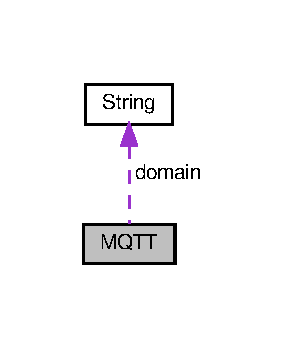
\includegraphics[width=137pt]{class_m_q_t_t__coll__graph}
\end{center}
\end{figure}
\subsection*{Public Types}
\begin{DoxyCompactItemize}
\item 
enum \textbf{ E\+M\+Q\+T\+T\+\_\+\+Q\+OS} \{ \textbf{ Q\+O\+S0} = 0, 
\textbf{ Q\+O\+S1} = 1, 
\textbf{ Q\+O\+S2} = 2
 \}
\item 
enum \textbf{ M\+Q\+T\+T\+\_\+\+V\+E\+R\+S\+I\+ON} \{ \textbf{ M\+Q\+T\+T\+\_\+\+V31} = 3, 
\textbf{ M\+Q\+T\+T\+\_\+\+V311} = 4
 \}
\item 
enum \textbf{ E\+M\+Q\+T\+T\+\_\+\+C\+O\+N\+N\+A\+C\+K\+\_\+\+R\+E\+S\+P\+O\+N\+SE} \{ \newline
\textbf{ C\+O\+N\+N\+\_\+\+A\+C\+C\+E\+PT} = 0, 
\textbf{ C\+O\+N\+N\+\_\+\+U\+N\+A\+C\+C\+E\+P\+T\+A\+B\+L\+E\+\_\+\+P\+R\+O\+C\+O\+T\+OL} = 1, 
\textbf{ C\+O\+N\+N\+\_\+\+I\+D\+\_\+\+R\+E\+J\+E\+CT} = 2, 
\textbf{ C\+O\+N\+N\+\_\+\+S\+E\+R\+V\+E\+R\+\_\+\+U\+N\+A\+V\+A\+I\+L\+A\+LE} = 3, 
\newline
\textbf{ C\+O\+N\+N\+\_\+\+B\+A\+D\+\_\+\+U\+S\+E\+R\+\_\+\+P\+A\+S\+S\+W\+O\+RD} = 4, 
\textbf{ C\+O\+N\+N\+\_\+\+N\+O\+T\+\_\+\+A\+U\+T\+H\+O\+R\+I\+Z\+ED} = 5
 \}
\end{DoxyCompactItemize}
\subsection*{Public Member Functions}
\begin{DoxyCompactItemize}
\item 
\textbf{ M\+Q\+TT} ()
\item 
\textbf{ M\+Q\+TT} (char $\ast$\textbf{ domain}, uint16\+\_\+t \textbf{ port}, void($\ast$\textbf{ callback})(char $\ast$, uint8\+\_\+t $\ast$, unsigned int))
\item 
\textbf{ M\+Q\+TT} (char $\ast$\textbf{ domain}, uint16\+\_\+t \textbf{ port}, void($\ast$\textbf{ callback})(char $\ast$, uint8\+\_\+t $\ast$, unsigned int), int \textbf{ maxpacketsize})
\item 
\textbf{ M\+Q\+TT} (uint8\+\_\+t $\ast$\textbf{ ip}, uint16\+\_\+t \textbf{ port}, void($\ast$\textbf{ callback})(char $\ast$, uint8\+\_\+t $\ast$, unsigned int))
\item 
\textbf{ M\+Q\+TT} (uint8\+\_\+t $\ast$\textbf{ ip}, uint16\+\_\+t \textbf{ port}, void($\ast$\textbf{ callback})(char $\ast$, uint8\+\_\+t $\ast$, unsigned int), int \textbf{ maxpacketsize})
\item 
\textbf{ M\+Q\+TT} (char $\ast$\textbf{ domain}, uint16\+\_\+t \textbf{ port}, int \textbf{ keepalive}, void($\ast$\textbf{ callback})(char $\ast$, uint8\+\_\+t $\ast$, unsigned int))
\item 
\textbf{ M\+Q\+TT} (char $\ast$\textbf{ domain}, uint16\+\_\+t \textbf{ port}, int \textbf{ keepalive}, void($\ast$\textbf{ callback})(char $\ast$, uint8\+\_\+t $\ast$, unsigned int), int \textbf{ maxpacketsize})
\item 
\textbf{ M\+Q\+TT} (uint8\+\_\+t $\ast$\textbf{ ip}, uint16\+\_\+t \textbf{ port}, int \textbf{ keepalive}, void($\ast$\textbf{ callback})(char $\ast$, uint8\+\_\+t $\ast$, unsigned int))
\item 
\textbf{ M\+Q\+TT} (uint8\+\_\+t $\ast$\textbf{ ip}, uint16\+\_\+t \textbf{ port}, int \textbf{ keepalive}, void($\ast$\textbf{ callback})(char $\ast$, uint8\+\_\+t $\ast$, unsigned int), int \textbf{ maxpacketsize})
\item 
\textbf{ $\sim$\+M\+Q\+TT} ()
\item 
void \textbf{ set\+Broker} (char $\ast$\textbf{ domain}, uint16\+\_\+t \textbf{ port})
\item 
void \textbf{ set\+Broker} (uint8\+\_\+t $\ast$\textbf{ ip}, uint16\+\_\+t \textbf{ port})
\item 
bool \textbf{ connect} (const char $\ast$id)
\item 
bool \textbf{ connect} (const char $\ast$id, const char $\ast$user, const char $\ast$pass)
\item 
bool \textbf{ connect} (const char $\ast$id, const char $\ast$user, const char $\ast$pass, const char $\ast$will\+Topic, \textbf{ E\+M\+Q\+T\+T\+\_\+\+Q\+OS} will\+Qos, uint8\+\_\+t will\+Retain, const char $\ast$will\+Message, bool clean\+Session, \textbf{ M\+Q\+T\+T\+\_\+\+V\+E\+R\+S\+I\+ON} version=\textbf{ M\+Q\+T\+T\+\_\+\+V311})
\item 
void \textbf{ disconnect} ()
\item 
void \textbf{ clear} ()
\item 
bool \textbf{ publish} (const char $\ast$topic, const char $\ast$payload)
\item 
bool \textbf{ publish} (const char $\ast$topic, const char $\ast$payload, bool retain)
\item 
bool \textbf{ publish} (const char $\ast$topic, const char $\ast$payload, \textbf{ E\+M\+Q\+T\+T\+\_\+\+Q\+OS} qos, uint16\+\_\+t $\ast$messageid=N\+U\+LL)
\item 
bool \textbf{ publish} (const char $\ast$topic, const char $\ast$payload, \textbf{ E\+M\+Q\+T\+T\+\_\+\+Q\+OS} qos, bool dup, uint16\+\_\+t $\ast$messageid=N\+U\+LL)
\item 
bool \textbf{ publish} (const char $\ast$topic, const uint8\+\_\+t $\ast$pyaload, unsigned int plength)
\item 
bool \textbf{ publish} (const char $\ast$topic, const uint8\+\_\+t $\ast$payload, unsigned int plength, \textbf{ E\+M\+Q\+T\+T\+\_\+\+Q\+OS} qos, uint16\+\_\+t $\ast$messageid=N\+U\+LL)
\item 
bool \textbf{ publish} (const char $\ast$topic, const uint8\+\_\+t $\ast$payload, unsigned int plength, \textbf{ E\+M\+Q\+T\+T\+\_\+\+Q\+OS} qos, bool dup, uint16\+\_\+t $\ast$messageid=N\+U\+LL)
\item 
bool \textbf{ publish} (const char $\ast$topic, const uint8\+\_\+t $\ast$payload, unsigned int plength, bool retain)
\item 
bool \textbf{ publish} (const char $\ast$topic, const uint8\+\_\+t $\ast$payload, unsigned int plength, bool retain, \textbf{ E\+M\+Q\+T\+T\+\_\+\+Q\+OS} qos, uint16\+\_\+t $\ast$messageid=N\+U\+LL)
\item 
bool \textbf{ publish} (const char $\ast$topic, const uint8\+\_\+t $\ast$payload, unsigned int plength, bool retain, \textbf{ E\+M\+Q\+T\+T\+\_\+\+Q\+OS} qos, bool dup, uint16\+\_\+t $\ast$messageid)
\item 
void \textbf{ add\+Qos\+Callback} (void($\ast$\textbf{ qoscallback})(unsigned int))
\item 
bool \textbf{ subscribe} (const char $\ast$topic)
\item 
bool \textbf{ subscribe} (const char $\ast$topic, \textbf{ E\+M\+Q\+T\+T\+\_\+\+Q\+OS})
\item 
bool \textbf{ unsubscribe} (const char $\ast$topic)
\item 
bool \textbf{ loop} ()
\item 
bool \textbf{ is\+Connected} ()
\end{DoxyCompactItemize}
\subsection*{Private Member Functions}
\begin{DoxyCompactItemize}
\item 
uint16\+\_\+t \textbf{ read\+Packet} (uint8\+\_\+t $\ast$)
\item 
uint8\+\_\+t \textbf{ read\+Byte} ()
\item 
bool \textbf{ write} (uint8\+\_\+t header, uint8\+\_\+t $\ast$buf, uint16\+\_\+t length)
\item 
uint16\+\_\+t \textbf{ write\+String} (const char $\ast$string, uint8\+\_\+t $\ast$buf, uint16\+\_\+t pos)
\item 
void \textbf{ initialize} (char $\ast$\textbf{ domain}, uint8\+\_\+t $\ast$\textbf{ ip}, uint16\+\_\+t \textbf{ port}, int \textbf{ keepalive}, void($\ast$\textbf{ callback})(char $\ast$, uint8\+\_\+t $\ast$, unsigned int), int \textbf{ maxpacketsize})
\item 
bool \textbf{ publish\+Release} (uint16\+\_\+t messageid)
\item 
bool \textbf{ publish\+Complete} (uint16\+\_\+t messageid)
\end{DoxyCompactItemize}
\subsection*{Private Attributes}
\begin{DoxyCompactItemize}
\item 
T\+C\+P\+Client \textbf{ \+\_\+client}
\item 
uint8\+\_\+t $\ast$ \textbf{ buffer} = N\+U\+LL
\item 
uint16\+\_\+t \textbf{ next\+Msg\+Id}
\item 
unsigned long \textbf{ last\+Out\+Activity}
\item 
unsigned long \textbf{ last\+In\+Activity}
\item 
bool \textbf{ ping\+Outstanding}
\item 
void($\ast$ \textbf{ callback} )(char $\ast$, uint8\+\_\+t $\ast$, unsigned int)
\item 
void($\ast$ \textbf{ qoscallback} )(unsigned int)
\item 
\textbf{ String} \textbf{ domain}
\item 
uint8\+\_\+t $\ast$ \textbf{ ip} = N\+U\+LL
\item 
uint16\+\_\+t \textbf{ port}
\item 
int \textbf{ keepalive}
\item 
uint16\+\_\+t \textbf{ maxpacketsize}
\end{DoxyCompactItemize}


\subsection{Detailed Description}


Definition at line 105 of file M\+Q\+T\+T.\+h.



\subsection{Member Enumeration Documentation}
\mbox{\label{class_m_q_t_t_a83c67833cdf6dfead0d42e6b48dae8bc}} 
\index{M\+Q\+TT@{M\+Q\+TT}!E\+M\+Q\+T\+T\+\_\+\+C\+O\+N\+N\+A\+C\+K\+\_\+\+R\+E\+S\+P\+O\+N\+SE@{E\+M\+Q\+T\+T\+\_\+\+C\+O\+N\+N\+A\+C\+K\+\_\+\+R\+E\+S\+P\+O\+N\+SE}}
\index{E\+M\+Q\+T\+T\+\_\+\+C\+O\+N\+N\+A\+C\+K\+\_\+\+R\+E\+S\+P\+O\+N\+SE@{E\+M\+Q\+T\+T\+\_\+\+C\+O\+N\+N\+A\+C\+K\+\_\+\+R\+E\+S\+P\+O\+N\+SE}!M\+Q\+TT@{M\+Q\+TT}}
\subsubsection{E\+M\+Q\+T\+T\+\_\+\+C\+O\+N\+N\+A\+C\+K\+\_\+\+R\+E\+S\+P\+O\+N\+SE}
{\footnotesize\ttfamily enum \textbf{ M\+Q\+T\+T\+::\+E\+M\+Q\+T\+T\+\_\+\+C\+O\+N\+N\+A\+C\+K\+\_\+\+R\+E\+S\+P\+O\+N\+SE}}

\begin{DoxyEnumFields}{Enumerator}
\raisebox{\heightof{T}}[0pt][0pt]{\index{C\+O\+N\+N\+\_\+\+A\+C\+C\+E\+PT@{C\+O\+N\+N\+\_\+\+A\+C\+C\+E\+PT}!M\+Q\+TT@{M\+Q\+TT}}\index{M\+Q\+TT@{M\+Q\+TT}!C\+O\+N\+N\+\_\+\+A\+C\+C\+E\+PT@{C\+O\+N\+N\+\_\+\+A\+C\+C\+E\+PT}}}\mbox{\label{class_m_q_t_t_a83c67833cdf6dfead0d42e6b48dae8bca10b54b970868dd657f962f3e0211c51a}} 
C\+O\+N\+N\+\_\+\+A\+C\+C\+E\+PT&\\
\hline

\raisebox{\heightof{T}}[0pt][0pt]{\index{C\+O\+N\+N\+\_\+\+U\+N\+A\+C\+C\+E\+P\+T\+A\+B\+L\+E\+\_\+\+P\+R\+O\+C\+O\+T\+OL@{C\+O\+N\+N\+\_\+\+U\+N\+A\+C\+C\+E\+P\+T\+A\+B\+L\+E\+\_\+\+P\+R\+O\+C\+O\+T\+OL}!M\+Q\+TT@{M\+Q\+TT}}\index{M\+Q\+TT@{M\+Q\+TT}!C\+O\+N\+N\+\_\+\+U\+N\+A\+C\+C\+E\+P\+T\+A\+B\+L\+E\+\_\+\+P\+R\+O\+C\+O\+T\+OL@{C\+O\+N\+N\+\_\+\+U\+N\+A\+C\+C\+E\+P\+T\+A\+B\+L\+E\+\_\+\+P\+R\+O\+C\+O\+T\+OL}}}\mbox{\label{class_m_q_t_t_a83c67833cdf6dfead0d42e6b48dae8bcab926be43cd794bcff8effaca0e3df5a2}} 
C\+O\+N\+N\+\_\+\+U\+N\+A\+C\+C\+E\+P\+T\+A\+B\+L\+E\+\_\+\+P\+R\+O\+C\+O\+T\+OL&\\
\hline

\raisebox{\heightof{T}}[0pt][0pt]{\index{C\+O\+N\+N\+\_\+\+I\+D\+\_\+\+R\+E\+J\+E\+CT@{C\+O\+N\+N\+\_\+\+I\+D\+\_\+\+R\+E\+J\+E\+CT}!M\+Q\+TT@{M\+Q\+TT}}\index{M\+Q\+TT@{M\+Q\+TT}!C\+O\+N\+N\+\_\+\+I\+D\+\_\+\+R\+E\+J\+E\+CT@{C\+O\+N\+N\+\_\+\+I\+D\+\_\+\+R\+E\+J\+E\+CT}}}\mbox{\label{class_m_q_t_t_a83c67833cdf6dfead0d42e6b48dae8bcadfea79ffb19345af8eec727a2fab5ba7}} 
C\+O\+N\+N\+\_\+\+I\+D\+\_\+\+R\+E\+J\+E\+CT&\\
\hline

\raisebox{\heightof{T}}[0pt][0pt]{\index{C\+O\+N\+N\+\_\+\+S\+E\+R\+V\+E\+R\+\_\+\+U\+N\+A\+V\+A\+I\+L\+A\+LE@{C\+O\+N\+N\+\_\+\+S\+E\+R\+V\+E\+R\+\_\+\+U\+N\+A\+V\+A\+I\+L\+A\+LE}!M\+Q\+TT@{M\+Q\+TT}}\index{M\+Q\+TT@{M\+Q\+TT}!C\+O\+N\+N\+\_\+\+S\+E\+R\+V\+E\+R\+\_\+\+U\+N\+A\+V\+A\+I\+L\+A\+LE@{C\+O\+N\+N\+\_\+\+S\+E\+R\+V\+E\+R\+\_\+\+U\+N\+A\+V\+A\+I\+L\+A\+LE}}}\mbox{\label{class_m_q_t_t_a83c67833cdf6dfead0d42e6b48dae8bca3f3bbddc59683ce074489bdba3479314}} 
C\+O\+N\+N\+\_\+\+S\+E\+R\+V\+E\+R\+\_\+\+U\+N\+A\+V\+A\+I\+L\+A\+LE&\\
\hline

\raisebox{\heightof{T}}[0pt][0pt]{\index{C\+O\+N\+N\+\_\+\+B\+A\+D\+\_\+\+U\+S\+E\+R\+\_\+\+P\+A\+S\+S\+W\+O\+RD@{C\+O\+N\+N\+\_\+\+B\+A\+D\+\_\+\+U\+S\+E\+R\+\_\+\+P\+A\+S\+S\+W\+O\+RD}!M\+Q\+TT@{M\+Q\+TT}}\index{M\+Q\+TT@{M\+Q\+TT}!C\+O\+N\+N\+\_\+\+B\+A\+D\+\_\+\+U\+S\+E\+R\+\_\+\+P\+A\+S\+S\+W\+O\+RD@{C\+O\+N\+N\+\_\+\+B\+A\+D\+\_\+\+U\+S\+E\+R\+\_\+\+P\+A\+S\+S\+W\+O\+RD}}}\mbox{\label{class_m_q_t_t_a83c67833cdf6dfead0d42e6b48dae8bcaa51f8337e0cd58337a6d9de028f7ffc5}} 
C\+O\+N\+N\+\_\+\+B\+A\+D\+\_\+\+U\+S\+E\+R\+\_\+\+P\+A\+S\+S\+W\+O\+RD&\\
\hline

\raisebox{\heightof{T}}[0pt][0pt]{\index{C\+O\+N\+N\+\_\+\+N\+O\+T\+\_\+\+A\+U\+T\+H\+O\+R\+I\+Z\+ED@{C\+O\+N\+N\+\_\+\+N\+O\+T\+\_\+\+A\+U\+T\+H\+O\+R\+I\+Z\+ED}!M\+Q\+TT@{M\+Q\+TT}}\index{M\+Q\+TT@{M\+Q\+TT}!C\+O\+N\+N\+\_\+\+N\+O\+T\+\_\+\+A\+U\+T\+H\+O\+R\+I\+Z\+ED@{C\+O\+N\+N\+\_\+\+N\+O\+T\+\_\+\+A\+U\+T\+H\+O\+R\+I\+Z\+ED}}}\mbox{\label{class_m_q_t_t_a83c67833cdf6dfead0d42e6b48dae8bca2a9953af7d955ad4954e9836a03ee4fa}} 
C\+O\+N\+N\+\_\+\+N\+O\+T\+\_\+\+A\+U\+T\+H\+O\+R\+I\+Z\+ED&\\
\hline

\end{DoxyEnumFields}


Definition at line 119 of file M\+Q\+T\+T.\+h.


\begin{DoxyCode}
119              \{
120     CONN_ACCEPT = 0,
121     CONN_UNACCEPTABLE_PROCOTOL = 1,
122     CONN_ID_REJECT = 2,
123     CONN_SERVER_UNAVAILALE = 3,
124     CONN_BAD_USER_PASSWORD = 4,
125     CONN_NOT_AUTHORIZED = 5
126 \} EMQTT_CONNACK_RESPONSE;
\end{DoxyCode}
\mbox{\label{class_m_q_t_t_aff501e08e20ebf26b3272fcc0e7215ff}} 
\index{M\+Q\+TT@{M\+Q\+TT}!E\+M\+Q\+T\+T\+\_\+\+Q\+OS@{E\+M\+Q\+T\+T\+\_\+\+Q\+OS}}
\index{E\+M\+Q\+T\+T\+\_\+\+Q\+OS@{E\+M\+Q\+T\+T\+\_\+\+Q\+OS}!M\+Q\+TT@{M\+Q\+TT}}
\subsubsection{E\+M\+Q\+T\+T\+\_\+\+Q\+OS}
{\footnotesize\ttfamily enum \textbf{ M\+Q\+T\+T\+::\+E\+M\+Q\+T\+T\+\_\+\+Q\+OS}}

types \begin{DoxyEnumFields}{Enumerator}
\raisebox{\heightof{T}}[0pt][0pt]{\index{Q\+O\+S0@{Q\+O\+S0}!M\+Q\+TT@{M\+Q\+TT}}\index{M\+Q\+TT@{M\+Q\+TT}!Q\+O\+S0@{Q\+O\+S0}}}\mbox{\label{class_m_q_t_t_aff501e08e20ebf26b3272fcc0e7215ffa14dc14f3d6013dcbfb6a2d88f9245b81}} 
Q\+O\+S0&\\
\hline

\raisebox{\heightof{T}}[0pt][0pt]{\index{Q\+O\+S1@{Q\+O\+S1}!M\+Q\+TT@{M\+Q\+TT}}\index{M\+Q\+TT@{M\+Q\+TT}!Q\+O\+S1@{Q\+O\+S1}}}\mbox{\label{class_m_q_t_t_aff501e08e20ebf26b3272fcc0e7215ffa67190ba35b18fa3bcdc3b1c34256b8f7}} 
Q\+O\+S1&\\
\hline

\raisebox{\heightof{T}}[0pt][0pt]{\index{Q\+O\+S2@{Q\+O\+S2}!M\+Q\+TT@{M\+Q\+TT}}\index{M\+Q\+TT@{M\+Q\+TT}!Q\+O\+S2@{Q\+O\+S2}}}\mbox{\label{class_m_q_t_t_aff501e08e20ebf26b3272fcc0e7215ffa824da0ec0c31a8d2978980a4ac9f7eb2}} 
Q\+O\+S2&\\
\hline

\end{DoxyEnumFields}


Definition at line 108 of file M\+Q\+T\+T.\+h.


\begin{DoxyCode}
108              \{
109     QOS0 = 0,
110     QOS1 = 1,
111     QOS2 = 2,
112 \} EMQTT_QOS;
\end{DoxyCode}
\mbox{\label{class_m_q_t_t_a49430c9d6f68bbdc4e1bd039a6f5f97e}} 
\index{M\+Q\+TT@{M\+Q\+TT}!M\+Q\+T\+T\+\_\+\+V\+E\+R\+S\+I\+ON@{M\+Q\+T\+T\+\_\+\+V\+E\+R\+S\+I\+ON}}
\index{M\+Q\+T\+T\+\_\+\+V\+E\+R\+S\+I\+ON@{M\+Q\+T\+T\+\_\+\+V\+E\+R\+S\+I\+ON}!M\+Q\+TT@{M\+Q\+TT}}
\subsubsection{M\+Q\+T\+T\+\_\+\+V\+E\+R\+S\+I\+ON}
{\footnotesize\ttfamily enum \textbf{ M\+Q\+T\+T\+::\+M\+Q\+T\+T\+\_\+\+V\+E\+R\+S\+I\+ON}}

\begin{DoxyEnumFields}{Enumerator}
\raisebox{\heightof{T}}[0pt][0pt]{\index{M\+Q\+T\+T\+\_\+\+V31@{M\+Q\+T\+T\+\_\+\+V31}!M\+Q\+TT@{M\+Q\+TT}}\index{M\+Q\+TT@{M\+Q\+TT}!M\+Q\+T\+T\+\_\+\+V31@{M\+Q\+T\+T\+\_\+\+V31}}}\mbox{\label{class_m_q_t_t_a49430c9d6f68bbdc4e1bd039a6f5f97eaf955bab848df0e287c12f20b3af37885}} 
M\+Q\+T\+T\+\_\+\+V31&\\
\hline

\raisebox{\heightof{T}}[0pt][0pt]{\index{M\+Q\+T\+T\+\_\+\+V311@{M\+Q\+T\+T\+\_\+\+V311}!M\+Q\+TT@{M\+Q\+TT}}\index{M\+Q\+TT@{M\+Q\+TT}!M\+Q\+T\+T\+\_\+\+V311@{M\+Q\+T\+T\+\_\+\+V311}}}\mbox{\label{class_m_q_t_t_a49430c9d6f68bbdc4e1bd039a6f5f97eae61f66bbb0b315cf4cb7636684c68602}} 
M\+Q\+T\+T\+\_\+\+V311&\\
\hline

\end{DoxyEnumFields}


Definition at line 114 of file M\+Q\+T\+T.\+h.


\begin{DoxyCode}
114             \{
115     MQTT_V31 = 3,
116     MQTT_V311 = 4
117 \} MQTT_VERSION;
\end{DoxyCode}


\subsection{Constructor \& Destructor Documentation}
\mbox{\label{class_m_q_t_t_a75b5fb0489a6ecc75d75ed2362e60aef}} 
\index{M\+Q\+TT@{M\+Q\+TT}!M\+Q\+TT@{M\+Q\+TT}}
\index{M\+Q\+TT@{M\+Q\+TT}!M\+Q\+TT@{M\+Q\+TT}}
\subsubsection{M\+Q\+T\+T()\hspace{0.1cm}{\footnotesize\ttfamily [1/9]}}
{\footnotesize\ttfamily M\+Q\+T\+T\+::\+M\+Q\+TT (\begin{DoxyParamCaption}{ }\end{DoxyParamCaption})\hspace{0.3cm}{\ttfamily [inline]}}



Definition at line 152 of file M\+Q\+T\+T.\+h.


\begin{DoxyCode}
152 \{\};
\end{DoxyCode}
\mbox{\label{class_m_q_t_t_a2ef4121d54530e1ffc918f2b0e3cbdc4}} 
\index{M\+Q\+TT@{M\+Q\+TT}!M\+Q\+TT@{M\+Q\+TT}}
\index{M\+Q\+TT@{M\+Q\+TT}!M\+Q\+TT@{M\+Q\+TT}}
\subsubsection{M\+Q\+T\+T()\hspace{0.1cm}{\footnotesize\ttfamily [2/9]}}
{\footnotesize\ttfamily M\+Q\+T\+T\+::\+M\+Q\+TT (\begin{DoxyParamCaption}\item[{char $\ast$}]{domain,  }\item[{uint16\+\_\+t}]{port,  }\item[{void($\ast$)(char $\ast$, uint8\+\_\+t $\ast$, unsigned int)}]{callback }\end{DoxyParamCaption})}



Definition at line 12 of file M\+Q\+T\+T.\+cpp.



References initialize().


\begin{DoxyCode}
12                                                                                      \{
13     this->initialize(domain, NULL, port, MQTT_DEFAULT_KEEPALIVE, callback, 
      MQTT_MAX_PACKET_SIZE);
14 \}
\end{DoxyCode}
\mbox{\label{class_m_q_t_t_a95dc3446cd91fd3448c3fe3938a40f72}} 
\index{M\+Q\+TT@{M\+Q\+TT}!M\+Q\+TT@{M\+Q\+TT}}
\index{M\+Q\+TT@{M\+Q\+TT}!M\+Q\+TT@{M\+Q\+TT}}
\subsubsection{M\+Q\+T\+T()\hspace{0.1cm}{\footnotesize\ttfamily [3/9]}}
{\footnotesize\ttfamily M\+Q\+T\+T\+::\+M\+Q\+TT (\begin{DoxyParamCaption}\item[{char $\ast$}]{domain,  }\item[{uint16\+\_\+t}]{port,  }\item[{void($\ast$)(char $\ast$, uint8\+\_\+t $\ast$, unsigned int)}]{callback,  }\item[{int}]{maxpacketsize }\end{DoxyParamCaption})}



Definition at line 16 of file M\+Q\+T\+T.\+cpp.



References initialize().


\begin{DoxyCode}
16                                                                                                         \{
17     this->initialize(domain, NULL, port, MQTT_DEFAULT_KEEPALIVE, callback, 
      maxpacketsize);
18 \}
\end{DoxyCode}
\mbox{\label{class_m_q_t_t_a0e4560eca8b493628aed67f949b45d42}} 
\index{M\+Q\+TT@{M\+Q\+TT}!M\+Q\+TT@{M\+Q\+TT}}
\index{M\+Q\+TT@{M\+Q\+TT}!M\+Q\+TT@{M\+Q\+TT}}
\subsubsection{M\+Q\+T\+T()\hspace{0.1cm}{\footnotesize\ttfamily [4/9]}}
{\footnotesize\ttfamily M\+Q\+T\+T\+::\+M\+Q\+TT (\begin{DoxyParamCaption}\item[{uint8\+\_\+t $\ast$}]{ip,  }\item[{uint16\+\_\+t}]{port,  }\item[{void($\ast$)(char $\ast$, uint8\+\_\+t $\ast$, unsigned int)}]{callback }\end{DoxyParamCaption})}



Definition at line 20 of file M\+Q\+T\+T.\+cpp.



References initialize().


\begin{DoxyCode}
20                                                                                     \{
21     this->initialize(NULL, ip, port, MQTT_DEFAULT_KEEPALIVE, callback, 
      MQTT_MAX_PACKET_SIZE);
22 \}
\end{DoxyCode}
\mbox{\label{class_m_q_t_t_a39e00a946c41fbe9eb504577269569cc}} 
\index{M\+Q\+TT@{M\+Q\+TT}!M\+Q\+TT@{M\+Q\+TT}}
\index{M\+Q\+TT@{M\+Q\+TT}!M\+Q\+TT@{M\+Q\+TT}}
\subsubsection{M\+Q\+T\+T()\hspace{0.1cm}{\footnotesize\ttfamily [5/9]}}
{\footnotesize\ttfamily M\+Q\+T\+T\+::\+M\+Q\+TT (\begin{DoxyParamCaption}\item[{uint8\+\_\+t $\ast$}]{ip,  }\item[{uint16\+\_\+t}]{port,  }\item[{void($\ast$)(char $\ast$, uint8\+\_\+t $\ast$, unsigned int)}]{callback,  }\item[{int}]{maxpacketsize }\end{DoxyParamCaption})}



Definition at line 24 of file M\+Q\+T\+T.\+cpp.



References initialize().


\begin{DoxyCode}
24                                                                                                        \{
25     this->initialize(NULL, ip, port, MQTT_DEFAULT_KEEPALIVE, callback, 
      maxpacketsize);
26 \}
\end{DoxyCode}
\mbox{\label{class_m_q_t_t_a799fede50157a7573f43582ccd429b5e}} 
\index{M\+Q\+TT@{M\+Q\+TT}!M\+Q\+TT@{M\+Q\+TT}}
\index{M\+Q\+TT@{M\+Q\+TT}!M\+Q\+TT@{M\+Q\+TT}}
\subsubsection{M\+Q\+T\+T()\hspace{0.1cm}{\footnotesize\ttfamily [6/9]}}
{\footnotesize\ttfamily M\+Q\+T\+T\+::\+M\+Q\+TT (\begin{DoxyParamCaption}\item[{char $\ast$}]{domain,  }\item[{uint16\+\_\+t}]{port,  }\item[{int}]{keepalive,  }\item[{void($\ast$)(char $\ast$, uint8\+\_\+t $\ast$, unsigned int)}]{callback }\end{DoxyParamCaption})}



Definition at line 28 of file M\+Q\+T\+T.\+cpp.



References initialize().


\begin{DoxyCode}
28                                                                                                     \{
29     this->initialize(domain, NULL, port, keepalive, callback, 
      MQTT_MAX_PACKET_SIZE);
30 \}
\end{DoxyCode}
\mbox{\label{class_m_q_t_t_a418f1aaefd9ebb233358a532d82d2307}} 
\index{M\+Q\+TT@{M\+Q\+TT}!M\+Q\+TT@{M\+Q\+TT}}
\index{M\+Q\+TT@{M\+Q\+TT}!M\+Q\+TT@{M\+Q\+TT}}
\subsubsection{M\+Q\+T\+T()\hspace{0.1cm}{\footnotesize\ttfamily [7/9]}}
{\footnotesize\ttfamily M\+Q\+T\+T\+::\+M\+Q\+TT (\begin{DoxyParamCaption}\item[{char $\ast$}]{domain,  }\item[{uint16\+\_\+t}]{port,  }\item[{int}]{keepalive,  }\item[{void($\ast$)(char $\ast$, uint8\+\_\+t $\ast$, unsigned int)}]{callback,  }\item[{int}]{maxpacketsize }\end{DoxyParamCaption})}



Definition at line 32 of file M\+Q\+T\+T.\+cpp.



References initialize().


\begin{DoxyCode}
32                                                                                                            
                  \{
33     this->initialize(domain, NULL, port, keepalive, callback, maxpacketsize);
34 \}
\end{DoxyCode}
\mbox{\label{class_m_q_t_t_ad68f2a18a197fa8944e8cc8e1950af5a}} 
\index{M\+Q\+TT@{M\+Q\+TT}!M\+Q\+TT@{M\+Q\+TT}}
\index{M\+Q\+TT@{M\+Q\+TT}!M\+Q\+TT@{M\+Q\+TT}}
\subsubsection{M\+Q\+T\+T()\hspace{0.1cm}{\footnotesize\ttfamily [8/9]}}
{\footnotesize\ttfamily M\+Q\+T\+T\+::\+M\+Q\+TT (\begin{DoxyParamCaption}\item[{uint8\+\_\+t $\ast$}]{ip,  }\item[{uint16\+\_\+t}]{port,  }\item[{int}]{keepalive,  }\item[{void($\ast$)(char $\ast$, uint8\+\_\+t $\ast$, unsigned int)}]{callback }\end{DoxyParamCaption})}



Definition at line 36 of file M\+Q\+T\+T.\+cpp.



References initialize().


\begin{DoxyCode}
36                                                                                                    \{
37     this->initialize(NULL, ip, port, keepalive, callback, MQTT_MAX_PACKET_SIZE);
38 \}
\end{DoxyCode}
\mbox{\label{class_m_q_t_t_a86aa31266ec2193bdd166e9fcd8c9d79}} 
\index{M\+Q\+TT@{M\+Q\+TT}!M\+Q\+TT@{M\+Q\+TT}}
\index{M\+Q\+TT@{M\+Q\+TT}!M\+Q\+TT@{M\+Q\+TT}}
\subsubsection{M\+Q\+T\+T()\hspace{0.1cm}{\footnotesize\ttfamily [9/9]}}
{\footnotesize\ttfamily M\+Q\+T\+T\+::\+M\+Q\+TT (\begin{DoxyParamCaption}\item[{uint8\+\_\+t $\ast$}]{ip,  }\item[{uint16\+\_\+t}]{port,  }\item[{int}]{keepalive,  }\item[{void($\ast$)(char $\ast$, uint8\+\_\+t $\ast$, unsigned int)}]{callback,  }\item[{int}]{maxpacketsize }\end{DoxyParamCaption})}



Definition at line 40 of file M\+Q\+T\+T.\+cpp.



References initialize().


\begin{DoxyCode}
40                                                                                                            
                 \{
41     this->initialize(NULL, ip, port, keepalive, callback, maxpacketsize);
42 \}
\end{DoxyCode}
\mbox{\label{class_m_q_t_t_a07b8f99719144b5d3bc8d8d817de3e8e}} 
\index{M\+Q\+TT@{M\+Q\+TT}!````~M\+Q\+TT@{$\sim$\+M\+Q\+TT}}
\index{````~M\+Q\+TT@{$\sim$\+M\+Q\+TT}!M\+Q\+TT@{M\+Q\+TT}}
\subsubsection{$\sim$\+M\+Q\+T\+T()}
{\footnotesize\ttfamily M\+Q\+T\+T\+::$\sim$\+M\+Q\+TT (\begin{DoxyParamCaption}{ }\end{DoxyParamCaption})}



Definition at line 44 of file M\+Q\+T\+T.\+cpp.



References buffer, disconnect(), and is\+Connected().


\begin{DoxyCode}
44             \{
45     \textcolor{keywordflow}{if} (isConnected()) \{
46         disconnect();
47     \}
48 
49     \textcolor{keywordflow}{if} (buffer != NULL)
50       \textcolor{keyword}{delete}[] buffer;
51 \}
\end{DoxyCode}


\subsection{Member Function Documentation}
\mbox{\label{class_m_q_t_t_a324c79ef8a1bfaf03d7b3e73b957283b}} 
\index{M\+Q\+TT@{M\+Q\+TT}!add\+Qos\+Callback@{add\+Qos\+Callback}}
\index{add\+Qos\+Callback@{add\+Qos\+Callback}!M\+Q\+TT@{M\+Q\+TT}}
\subsubsection{add\+Qos\+Callback()}
{\footnotesize\ttfamily void M\+Q\+T\+T\+::add\+Qos\+Callback (\begin{DoxyParamCaption}\item[{void($\ast$)(unsigned int)}]{qoscallback }\end{DoxyParamCaption})}



Definition at line 89 of file M\+Q\+T\+T.\+cpp.



References qoscallback.


\begin{DoxyCode}
89                                                            \{
90     this->qoscallback = qoscallback;
91 \}
\end{DoxyCode}
\mbox{\label{class_m_q_t_t_a510932d1c5fb0c918debcf60cfc267e1}} 
\index{M\+Q\+TT@{M\+Q\+TT}!clear@{clear}}
\index{clear@{clear}!M\+Q\+TT@{M\+Q\+TT}}
\subsubsection{clear()}
{\footnotesize\ttfamily void M\+Q\+T\+T\+::clear (\begin{DoxyParamCaption}{ }\end{DoxyParamCaption})}



Definition at line 534 of file M\+Q\+T\+T.\+cpp.


\begin{DoxyCode}
534                  \{
535   _client.stop();
536   lastInActivity = lastOutActivity = millis();
537 \}
\end{DoxyCode}
\mbox{\label{class_m_q_t_t_ae76d538b01191df33610a950bf4e9717}} 
\index{M\+Q\+TT@{M\+Q\+TT}!connect@{connect}}
\index{connect@{connect}!M\+Q\+TT@{M\+Q\+TT}}
\subsubsection{connect()\hspace{0.1cm}{\footnotesize\ttfamily [1/3]}}
{\footnotesize\ttfamily bool M\+Q\+T\+T\+::connect (\begin{DoxyParamCaption}\item[{const char $\ast$}]{id }\end{DoxyParamCaption})}



Definition at line 94 of file M\+Q\+T\+T.\+cpp.



References connect(), and Q\+O\+S0.


\begin{DoxyCode}
94                                  \{
95     \textcolor{keywordflow}{return} connect(\textcolor{keywordtype}{id}, NULL, NULL, 0, QOS0, 0, 0, \textcolor{keyword}{true});
96 \}
\end{DoxyCode}
\mbox{\label{class_m_q_t_t_a280e592fced51964607c66f7ab450b46}} 
\index{M\+Q\+TT@{M\+Q\+TT}!connect@{connect}}
\index{connect@{connect}!M\+Q\+TT@{M\+Q\+TT}}
\subsubsection{connect()\hspace{0.1cm}{\footnotesize\ttfamily [2/3]}}
{\footnotesize\ttfamily bool M\+Q\+T\+T\+::connect (\begin{DoxyParamCaption}\item[{const char $\ast$}]{id,  }\item[{const char $\ast$}]{user,  }\item[{const char $\ast$}]{pass }\end{DoxyParamCaption})}



Definition at line 98 of file M\+Q\+T\+T.\+cpp.



References connect(), and Q\+O\+S0.


\begin{DoxyCode}
98                                                                      \{
99     \textcolor{keywordflow}{return} connect(\textcolor{keywordtype}{id}, user, pass, 0, QOS0, 0, 0, \textcolor{keyword}{true});
100 \}
\end{DoxyCode}
\mbox{\label{class_m_q_t_t_aa880316318b5bdc133c2f8c6bba1e253}} 
\index{M\+Q\+TT@{M\+Q\+TT}!connect@{connect}}
\index{connect@{connect}!M\+Q\+TT@{M\+Q\+TT}}
\subsubsection{connect()\hspace{0.1cm}{\footnotesize\ttfamily [3/3]}}
{\footnotesize\ttfamily bool M\+Q\+T\+T\+::connect (\begin{DoxyParamCaption}\item[{const char $\ast$}]{id,  }\item[{const char $\ast$}]{user,  }\item[{const char $\ast$}]{pass,  }\item[{const char $\ast$}]{will\+Topic,  }\item[{\textbf{ E\+M\+Q\+T\+T\+\_\+\+Q\+OS}}]{will\+Qos,  }\item[{uint8\+\_\+t}]{will\+Retain,  }\item[{const char $\ast$}]{will\+Message,  }\item[{bool}]{clean\+Session,  }\item[{\textbf{ M\+Q\+T\+T\+\_\+\+V\+E\+R\+S\+I\+ON}}]{version = {\ttfamily \textbf{ M\+Q\+T\+T\+\_\+\+V311}} }\end{DoxyParamCaption})}



Definition at line 102 of file M\+Q\+T\+T.\+cpp.



References buffer, C\+O\+N\+N\+\_\+\+A\+C\+C\+E\+PT, is\+Connected(), keepalive, M\+Q\+T\+T\+\_\+\+V31, M\+Q\+T\+T\+\_\+\+V311, next\+Msg\+Id, ping\+Outstanding, read\+Packet(), write(), and write\+String().



Referenced by connect().


\begin{DoxyCode}
102                                                                                                            
                                                                                                \{
103     \textcolor{keywordflow}{if} (!isConnected()) \{
104         \textcolor{keywordtype}{int} result = 0;
105         \textcolor{keywordflow}{if} (ip == NULL)
106             result = _client.connect(this->domain.c_str(), this->port);
107         \textcolor{keywordflow}{else}
108             result = _client.connect(this->ip, this->port);
109 
110         \textcolor{keywordflow}{if} (result) \{
111             nextMsgId = 1;
112             uint16\_t length = 5;
113 
114             \textcolor{keywordflow}{if} (version == MQTT_V311) \{
115                 \textcolor{keyword}{const} uint8\_t MQTT\_HEADER\_V311[] = \{0x00,0x04,\textcolor{charliteral}{'M'},\textcolor{charliteral}{'Q'},\textcolor{charliteral}{'T'},\textcolor{charliteral}{'T'},
      MQTT_V311\};
116                 memcpy(buffer + length, MQTT\_HEADER\_V311, \textcolor{keyword}{sizeof}(MQTT\_HEADER\_V311));
117                 length+=\textcolor{keyword}{sizeof}(MQTT\_HEADER\_V311);
118             \} \textcolor{keywordflow}{else} \{
119                 \textcolor{keyword}{const} uint8\_t MQTT\_HEADER\_V31[] = \{0x00,0x06,\textcolor{charliteral}{'M'},\textcolor{charliteral}{'Q'},\textcolor{charliteral}{'I'},\textcolor{charliteral}{'s'},\textcolor{charliteral}{'d'},\textcolor{charliteral}{'p'}, 
      MQTT_V31\};
120                 memcpy(buffer + length, MQTT\_HEADER\_V31, \textcolor{keyword}{sizeof}(MQTT\_HEADER\_V31));
121                 length+=\textcolor{keyword}{sizeof}(MQTT\_HEADER\_V31);
122             \}
123 
124             uint8\_t v = 0;
125             \textcolor{keywordflow}{if} (willTopic) \{
126                 v = 0x06|(willQos<<3)|(willRetain<<5);
127             \} \textcolor{keywordflow}{else} \{
128                 v = 0x02;
129             \}
130 
131             \textcolor{keywordflow}{if} (!cleanSession) \{
132               v = v&0xfd;
133             \}
134 
135             \textcolor{keywordflow}{if}(user != NULL) \{
136                 v = v|0x80;
137 
138                 \textcolor{keywordflow}{if}(pass != NULL) \{
139                     v = v|(0x80>>1);
140                 \}
141             \}
142 
143             buffer[length++] = v;
144 
145             buffer[length++] = ((this->keepalive) >> 8);
146             buffer[length++] = ((this->keepalive) & 0xFF);
147             length = writeString(\textcolor{keywordtype}{id}, buffer, length);
148             \textcolor{keywordflow}{if} (willTopic) \{
149                 length = writeString(willTopic, buffer, length);
150                 length = writeString(willMessage, buffer, length);
151             \}
152 
153             \textcolor{keywordflow}{if}(user != NULL) \{
154                 length = writeString(user,buffer,length);
155                 \textcolor{keywordflow}{if}(pass != NULL) \{
156                     length = writeString(pass,buffer,length);
157                 \}
158             \}
159 
160             write(MQTTCONNECT, buffer, length-5);
161             lastInActivity = lastOutActivity = millis();
162 
163             \textcolor{keywordflow}{while} (!_client.available()) \{
164                 \textcolor{keywordtype}{unsigned} \textcolor{keywordtype}{long} t = millis();
165                 \textcolor{keywordflow}{if} (t-lastInActivity > this->keepalive*1000UL) \{
166                     _client.stop();
167                     \textcolor{keywordflow}{return} \textcolor{keyword}{false};
168                 \}
169             \}
170             uint8\_t llen;
171             uint16\_t len = readPacket(&llen);
172 
173             \textcolor{keywordflow}{if} (len == 4) \{
174                 \textcolor{keywordflow}{if} (buffer[3] == CONN_ACCEPT) \{
175                     lastInActivity = millis();
176                     pingOutstanding = \textcolor{keyword}{false};
177                     debug_print(\textcolor{stringliteral}{" Connect success\(\backslash\)n"});
178                     \textcolor{keywordflow}{return} \textcolor{keyword}{true};
179                 \} \textcolor{keywordflow}{else} \{
180                     \textcolor{comment}{// check EMQTT\_CONNACK\_RESPONSE code.}
181                     debug_print(\textcolor{stringliteral}{" Connect fail. code = [%d]\(\backslash\)n"}, buffer[3]);
182                 \}
183             \}
184         \}
185         _client.stop();
186     \}
187     \textcolor{keywordflow}{return} \textcolor{keyword}{false};
188 \}
\end{DoxyCode}
\mbox{\label{class_m_q_t_t_a7d49b425517408d227836c10169f8df8}} 
\index{M\+Q\+TT@{M\+Q\+TT}!disconnect@{disconnect}}
\index{disconnect@{disconnect}!M\+Q\+TT@{M\+Q\+TT}}
\subsubsection{disconnect()}
{\footnotesize\ttfamily void M\+Q\+T\+T\+::disconnect (\begin{DoxyParamCaption}{ }\end{DoxyParamCaption})}



Definition at line 506 of file M\+Q\+T\+T.\+cpp.



References buffer.



Referenced by set\+Broker(), and $\sim$\+M\+Q\+T\+T().


\begin{DoxyCode}
506                       \{
507     buffer[0] = MQTTDISCONNECT;
508     buffer[1] = 0;
509     _client.write(buffer,2);
510     _client.stop();
511     lastInActivity = lastOutActivity = millis();
512 \}
\end{DoxyCode}
\mbox{\label{class_m_q_t_t_a849de76aa2a1f4b89c1b4a8dfb7c3661}} 
\index{M\+Q\+TT@{M\+Q\+TT}!initialize@{initialize}}
\index{initialize@{initialize}!M\+Q\+TT@{M\+Q\+TT}}
\subsubsection{initialize()}
{\footnotesize\ttfamily void M\+Q\+T\+T\+::initialize (\begin{DoxyParamCaption}\item[{char $\ast$}]{domain,  }\item[{uint8\+\_\+t $\ast$}]{ip,  }\item[{uint16\+\_\+t}]{port,  }\item[{int}]{keepalive,  }\item[{void($\ast$)(char $\ast$, uint8\+\_\+t $\ast$, unsigned int)}]{callback,  }\item[{int}]{maxpacketsize }\end{DoxyParamCaption})\hspace{0.3cm}{\ttfamily [private]}}



Definition at line 53 of file M\+Q\+T\+T.\+cpp.



References buffer, callback, domain, ip, keepalive, maxpacketsize, String\+::operator=(), port, and qoscallback.



Referenced by M\+Q\+T\+T().


\begin{DoxyCode}
53                                                                                                            
                                          \{
54     this->callback = callback;
55     this->qoscallback = NULL;
56     \textcolor{keywordflow}{if} (ip != NULL)
57         this->ip = ip;
58     \textcolor{keywordflow}{if} (domain != NULL)
59         this->domain = domain;
60     this->port = port;
61     this->keepalive = keepalive;
62 
63     \textcolor{comment}{// if maxpacketsize is over MQTT\_MAX\_PACKET\_SIZE.}
64     this->maxpacketsize = (maxpacketsize <= MQTT_MAX_PACKET_SIZE ? 
      MQTT_MAX_PACKET_SIZE : maxpacketsize);
65     \textcolor{keywordflow}{if} (buffer != NULL)
66       \textcolor{keyword}{delete}[] buffer;
67     buffer = \textcolor{keyword}{new} uint8\_t[this->maxpacketsize];
68 \}
\end{DoxyCode}
\mbox{\label{class_m_q_t_t_a57a5231fd3205682c56de70e57dd9d62}} 
\index{M\+Q\+TT@{M\+Q\+TT}!is\+Connected@{is\+Connected}}
\index{is\+Connected@{is\+Connected}!M\+Q\+TT@{M\+Q\+TT}}
\subsubsection{is\+Connected()}
{\footnotesize\ttfamily bool M\+Q\+T\+T\+::is\+Connected (\begin{DoxyParamCaption}{ }\end{DoxyParamCaption})}



Definition at line 528 of file M\+Q\+T\+T.\+cpp.



Referenced by connect(), loop(), publish(), publish\+Complete(), publish\+Release(), set\+Broker(), subscribe(), unsubscribe(), and $\sim$\+M\+Q\+T\+T().


\begin{DoxyCode}
528                        \{
529     \textcolor{keywordtype}{bool} rc = (int)_client.connected();
530     \textcolor{keywordflow}{if} (!rc) _client.stop();
531     \textcolor{keywordflow}{return} rc;
532 \}
\end{DoxyCode}
\mbox{\label{class_m_q_t_t_a5f9624e440c99d7ec0fb0a8c1a30d064}} 
\index{M\+Q\+TT@{M\+Q\+TT}!loop@{loop}}
\index{loop@{loop}!M\+Q\+TT@{M\+Q\+TT}}
\subsubsection{loop()}
{\footnotesize\ttfamily bool M\+Q\+T\+T\+::loop (\begin{DoxyParamCaption}{ }\end{DoxyParamCaption})}



Definition at line 240 of file M\+Q\+T\+T.\+cpp.



References buffer, callback, is\+Connected(), keepalive, last\+In\+Activity, last\+Out\+Activity, ping\+Outstanding, publish\+Complete(), publish\+Release(), qoscallback, and read\+Packet().


\begin{DoxyCode}
240                 \{
241     \textcolor{keywordflow}{if} (isConnected()) \{
242         \textcolor{keywordtype}{unsigned} \textcolor{keywordtype}{long} t = millis();
243         \textcolor{keywordflow}{if} ((t - lastInActivity > this->keepalive*1000UL) || (t - 
      lastOutActivity > this->keepalive*1000UL)) \{
244             \textcolor{keywordflow}{if} (pingOutstanding) \{
245                 _client.stop();
246                 \textcolor{keywordflow}{return} \textcolor{keyword}{false};
247             \} \textcolor{keywordflow}{else} \{
248                 buffer[0] = MQTTPINGREQ;
249                 buffer[1] = 0;
250                 _client.write(buffer,2);
251                 lastOutActivity = t;
252                 lastInActivity = t;
253                 pingOutstanding = \textcolor{keyword}{true};
254             \}
255         \}
256         \textcolor{keywordflow}{if} (_client.available()) \{
257             uint8\_t llen;
258             uint16\_t len = readPacket(&llen);
259             uint16\_t msgId = 0;
260             uint8\_t *payload;
261             \textcolor{keywordflow}{if} (len > 0) \{
262                 lastInActivity = t;
263                 uint8\_t type = buffer[0]&0xF0;
264                 \textcolor{keywordflow}{if} (type == MQTTPUBLISH) \{
265                     \textcolor{keywordflow}{if} (callback) \{
266                         uint16\_t tl = (buffer[llen+1]<<8)+buffer[llen+2]; \textcolor{comment}{// topic length}
267                         \textcolor{keywordtype}{char} topic[tl+1];
268                         \textcolor{keywordflow}{for} (uint16\_t i=0;i<tl;i++) \{
269                             topic[i] = buffer[llen+3+i];
270                         \}
271                         topic[tl] = 0;
272                         \textcolor{comment}{// msgId only present for QOS>0}
273                         \textcolor{keywordflow}{if} ((buffer[0]&0x06) == MQTTQOS1_HEADER_MASK) \{ \textcolor{comment}{// QoS=1}
274                             msgId = (buffer[llen+3+tl]<<8)+buffer[llen+3+tl+1];
275                             payload = buffer+llen+3+tl+2;
276                             callback(topic,payload,len-llen-3-tl-2);
277 
278                             buffer[0] = MQTTPUBACK; \textcolor{comment}{// respond with PUBACK}
279                             buffer[1] = 2;
280                             buffer[2] = (msgId >> 8);
281                             buffer[3] = (msgId & 0xFF);
282                             _client.write(buffer,4);
283                             lastOutActivity = t;
284                                     \} \textcolor{keywordflow}{else} \textcolor{keywordflow}{if} ((buffer[0] & 0x06) == 
      MQTTQOS2_HEADER_MASK) \{ \textcolor{comment}{// QoS=2}
285                                           msgId = (buffer[llen + 3 + tl] << 8) + 
      buffer[llen + 3 + tl + 1];
286                                           payload = buffer + llen + 3 + tl + 2;
287                                           callback(topic, payload, len - llen - 3 - tl - 2);
288 
289                                         buffer[0] = MQTTPUBREC; \textcolor{comment}{// respond with PUBREC}
290                                         buffer[1] = 2;
291                                         buffer[2] = (msgId >> 8);
292                                         buffer[3] = (msgId & 0xFF);
293                                         _client.write(buffer, 4);
294                                         lastOutActivity = t;
295                                     \} \textcolor{keywordflow}{else} \{
296                             payload = buffer+llen+3+tl;
297                             callback(topic,payload,len-llen-3-tl);
298                         \}
299                     \}
300                 \} \textcolor{keywordflow}{else} \textcolor{keywordflow}{if} (type == MQTTPUBREC) \{
301                     \textcolor{comment}{// check for the situation that QoS2 receive PUBREC, should return PUBREL}
302                     msgId = (buffer[2] << 8) + buffer[3];
303                     this->publishRelease(msgId);
304                 \} \textcolor{keywordflow}{else} \textcolor{keywordflow}{if} (type == MQTTPUBACK) \{
305                     \textcolor{keywordflow}{if} (qoscallback) \{
306                         \textcolor{comment}{// this case QOS==1}
307                         \textcolor{keywordflow}{if} (len == 4 && (buffer[0]&0x06) == MQTTQOS0_HEADER_MASK) \{
308                             msgId = (buffer[2]<<8)+buffer[3];
309                             this->qoscallback(msgId);
310                         \}
311                     \}
312                 \} \textcolor{keywordflow}{else} \textcolor{keywordflow}{if} (type == MQTTPUBREL) \{
313                   msgId = (buffer[2] << 8) + buffer[3];
314                   this->publishComplete(msgId);
315                 \} \textcolor{keywordflow}{else} \textcolor{keywordflow}{if} (type == MQTTPUBCOMP) \{
316                   \textcolor{keywordflow}{if} (qoscallback) \{
317                       \textcolor{comment}{// msgId only present for QOS==0}
318                       \textcolor{keywordflow}{if} (len == 4 && (buffer[0]&0x06) == MQTTQOS0_HEADER_MASK) \{
319                           msgId = (buffer[2]<<8)+buffer[3];
320                           this->qoscallback(msgId);
321                       \}
322                   \}
323                 \} \textcolor{keywordflow}{else} \textcolor{keywordflow}{if} (type == MQTTSUBACK) \{
324                     \textcolor{comment}{// if something...}
325                 \} \textcolor{keywordflow}{else} \textcolor{keywordflow}{if} (type == MQTTPINGREQ) \{
326                     buffer[0] = MQTTPINGRESP;
327                     buffer[1] = 0;
328                     _client.write(buffer,2);
329                 \} \textcolor{keywordflow}{else} \textcolor{keywordflow}{if} (type == MQTTPINGRESP) \{
330                     pingOutstanding = \textcolor{keyword}{false};
331                 \}
332             \}
333         \}
334         \textcolor{keywordflow}{return} \textcolor{keyword}{true};
335     \}
336     \textcolor{keywordflow}{return} \textcolor{keyword}{false};
337 \}
\end{DoxyCode}
\mbox{\label{class_m_q_t_t_a0a335a0e6c60ea0e256f76a1969a5137}} 
\index{M\+Q\+TT@{M\+Q\+TT}!publish@{publish}}
\index{publish@{publish}!M\+Q\+TT@{M\+Q\+TT}}
\subsubsection{publish()\hspace{0.1cm}{\footnotesize\ttfamily [1/10]}}
{\footnotesize\ttfamily bool M\+Q\+T\+T\+::publish (\begin{DoxyParamCaption}\item[{const char $\ast$}]{topic,  }\item[{const char $\ast$}]{payload }\end{DoxyParamCaption})}



Definition at line 339 of file M\+Q\+T\+T.\+cpp.



References publish(), and Q\+O\+S0.


\begin{DoxyCode}
339                                                          \{
340     \textcolor{keywordflow}{return} publish(topic, (uint8\_t*)payload, strlen(payload), \textcolor{keyword}{false}, QOS0, NULL);
341 \}
\end{DoxyCode}
\mbox{\label{class_m_q_t_t_a802136b5419b3a694ea88be27bdb9043}} 
\index{M\+Q\+TT@{M\+Q\+TT}!publish@{publish}}
\index{publish@{publish}!M\+Q\+TT@{M\+Q\+TT}}
\subsubsection{publish()\hspace{0.1cm}{\footnotesize\ttfamily [2/10]}}
{\footnotesize\ttfamily bool M\+Q\+T\+T\+::publish (\begin{DoxyParamCaption}\item[{const char $\ast$}]{topic,  }\item[{const char $\ast$}]{payload,  }\item[{bool}]{retain }\end{DoxyParamCaption})}



Definition at line 343 of file M\+Q\+T\+T.\+cpp.



References publish(), and Q\+O\+S0.


\begin{DoxyCode}
343                                                                       \{
344     \textcolor{keywordflow}{return} publish(topic, (uint8\_t*)payload, strlen(payload), retain, QOS0, NULL);
345 \}
\end{DoxyCode}
\mbox{\label{class_m_q_t_t_ae9321f0f8b365eaf32c87706273cb473}} 
\index{M\+Q\+TT@{M\+Q\+TT}!publish@{publish}}
\index{publish@{publish}!M\+Q\+TT@{M\+Q\+TT}}
\subsubsection{publish()\hspace{0.1cm}{\footnotesize\ttfamily [3/10]}}
{\footnotesize\ttfamily bool M\+Q\+T\+T\+::publish (\begin{DoxyParamCaption}\item[{const char $\ast$}]{topic,  }\item[{const char $\ast$}]{payload,  }\item[{\textbf{ E\+M\+Q\+T\+T\+\_\+\+Q\+OS}}]{qos,  }\item[{uint16\+\_\+t $\ast$}]{messageid = {\ttfamily NULL} }\end{DoxyParamCaption})}



Definition at line 351 of file M\+Q\+T\+T.\+cpp.



References publish().


\begin{DoxyCode}
351                                                                                               \{
352     \textcolor{keywordflow}{return} publish(topic, (uint8\_t*)payload, strlen(payload), \textcolor{keyword}{false}, qos, messageid);
353 \}
\end{DoxyCode}
\mbox{\label{class_m_q_t_t_abd5a453777652cd30ae3cfc4df4aa376}} 
\index{M\+Q\+TT@{M\+Q\+TT}!publish@{publish}}
\index{publish@{publish}!M\+Q\+TT@{M\+Q\+TT}}
\subsubsection{publish()\hspace{0.1cm}{\footnotesize\ttfamily [4/10]}}
{\footnotesize\ttfamily bool M\+Q\+T\+T\+::publish (\begin{DoxyParamCaption}\item[{const char $\ast$}]{topic,  }\item[{const char $\ast$}]{payload,  }\item[{\textbf{ E\+M\+Q\+T\+T\+\_\+\+Q\+OS}}]{qos,  }\item[{bool}]{dup,  }\item[{uint16\+\_\+t $\ast$}]{messageid = {\ttfamily NULL} }\end{DoxyParamCaption})}



Definition at line 347 of file M\+Q\+T\+T.\+cpp.



References publish().


\begin{DoxyCode}
347                                                                                                         \{
348     \textcolor{keywordflow}{return} publish(topic, (uint8\_t*)payload, strlen(payload), \textcolor{keyword}{false}, qos, dup, messageid);
349 \}
\end{DoxyCode}
\mbox{\label{class_m_q_t_t_a6a5dd9b7c19f2892802a222ec5d610b5}} 
\index{M\+Q\+TT@{M\+Q\+TT}!publish@{publish}}
\index{publish@{publish}!M\+Q\+TT@{M\+Q\+TT}}
\subsubsection{publish()\hspace{0.1cm}{\footnotesize\ttfamily [5/10]}}
{\footnotesize\ttfamily bool M\+Q\+T\+T\+::publish (\begin{DoxyParamCaption}\item[{const char $\ast$}]{topic,  }\item[{const uint8\+\_\+t $\ast$}]{pyaload,  }\item[{unsigned int}]{plength }\end{DoxyParamCaption})}



Definition at line 355 of file M\+Q\+T\+T.\+cpp.



References publish(), and Q\+O\+S0.


\begin{DoxyCode}
355                                                                                   \{
356     \textcolor{keywordflow}{return} publish(topic, payload, plength, \textcolor{keyword}{false}, QOS0, NULL);
357 \}
\end{DoxyCode}
\mbox{\label{class_m_q_t_t_ae9ea303a55434b8a6bba3147938aa9a9}} 
\index{M\+Q\+TT@{M\+Q\+TT}!publish@{publish}}
\index{publish@{publish}!M\+Q\+TT@{M\+Q\+TT}}
\subsubsection{publish()\hspace{0.1cm}{\footnotesize\ttfamily [6/10]}}
{\footnotesize\ttfamily bool M\+Q\+T\+T\+::publish (\begin{DoxyParamCaption}\item[{const char $\ast$}]{topic,  }\item[{const uint8\+\_\+t $\ast$}]{payload,  }\item[{unsigned int}]{plength,  }\item[{\textbf{ E\+M\+Q\+T\+T\+\_\+\+Q\+OS}}]{qos,  }\item[{uint16\+\_\+t $\ast$}]{messageid = {\ttfamily NULL} }\end{DoxyParamCaption})}



Definition at line 363 of file M\+Q\+T\+T.\+cpp.



References publish().


\begin{DoxyCode}
363                                                                                                            
                 \{
364     \textcolor{keywordflow}{return} publish(topic, payload, plength, \textcolor{keyword}{false}, qos, messageid);
365 \}
\end{DoxyCode}
\mbox{\label{class_m_q_t_t_a5e7738081e77b6c381f71737e8841869}} 
\index{M\+Q\+TT@{M\+Q\+TT}!publish@{publish}}
\index{publish@{publish}!M\+Q\+TT@{M\+Q\+TT}}
\subsubsection{publish()\hspace{0.1cm}{\footnotesize\ttfamily [7/10]}}
{\footnotesize\ttfamily bool M\+Q\+T\+T\+::publish (\begin{DoxyParamCaption}\item[{const char $\ast$}]{topic,  }\item[{const uint8\+\_\+t $\ast$}]{payload,  }\item[{unsigned int}]{plength,  }\item[{\textbf{ E\+M\+Q\+T\+T\+\_\+\+Q\+OS}}]{qos,  }\item[{bool}]{dup,  }\item[{uint16\+\_\+t $\ast$}]{messageid = {\ttfamily NULL} }\end{DoxyParamCaption})}



Definition at line 359 of file M\+Q\+T\+T.\+cpp.



References publish().


\begin{DoxyCode}
359                                                                                                            
                           \{
360     \textcolor{keywordflow}{return} publish(topic, payload, plength, \textcolor{keyword}{false}, qos, dup, messageid);
361 \}
\end{DoxyCode}
\mbox{\label{class_m_q_t_t_ac827a753cde9ed29783dc60092990072}} 
\index{M\+Q\+TT@{M\+Q\+TT}!publish@{publish}}
\index{publish@{publish}!M\+Q\+TT@{M\+Q\+TT}}
\subsubsection{publish()\hspace{0.1cm}{\footnotesize\ttfamily [8/10]}}
{\footnotesize\ttfamily bool M\+Q\+T\+T\+::publish (\begin{DoxyParamCaption}\item[{const char $\ast$}]{topic,  }\item[{const uint8\+\_\+t $\ast$}]{payload,  }\item[{unsigned int}]{plength,  }\item[{bool}]{retain }\end{DoxyParamCaption})}



Definition at line 367 of file M\+Q\+T\+T.\+cpp.



References publish(), and Q\+O\+S0.


\begin{DoxyCode}
367                                                                                                \{
368     \textcolor{keywordflow}{return} publish(topic, payload, plength, retain, QOS0, NULL);
369 \}
\end{DoxyCode}
\mbox{\label{class_m_q_t_t_a12d6e2ff5b2aadb36e2fd7abed4fa46b}} 
\index{M\+Q\+TT@{M\+Q\+TT}!publish@{publish}}
\index{publish@{publish}!M\+Q\+TT@{M\+Q\+TT}}
\subsubsection{publish()\hspace{0.1cm}{\footnotesize\ttfamily [9/10]}}
{\footnotesize\ttfamily bool M\+Q\+T\+T\+::publish (\begin{DoxyParamCaption}\item[{const char $\ast$}]{topic,  }\item[{const uint8\+\_\+t $\ast$}]{payload,  }\item[{unsigned int}]{plength,  }\item[{bool}]{retain,  }\item[{\textbf{ E\+M\+Q\+T\+T\+\_\+\+Q\+OS}}]{qos,  }\item[{uint16\+\_\+t $\ast$}]{messageid = {\ttfamily NULL} }\end{DoxyParamCaption})}



Definition at line 371 of file M\+Q\+T\+T.\+cpp.



References publish().



Referenced by publish().


\begin{DoxyCode}
371                                                                                                            
                              \{
372     \textcolor{keywordflow}{return} publish(topic, payload, plength, retain, qos, \textcolor{keyword}{false}, messageid);
373 \}
\end{DoxyCode}
\mbox{\label{class_m_q_t_t_a11b8368945d62d46acf4e7d41c57e3c3}} 
\index{M\+Q\+TT@{M\+Q\+TT}!publish@{publish}}
\index{publish@{publish}!M\+Q\+TT@{M\+Q\+TT}}
\subsubsection{publish()\hspace{0.1cm}{\footnotesize\ttfamily [10/10]}}
{\footnotesize\ttfamily bool M\+Q\+T\+T\+::publish (\begin{DoxyParamCaption}\item[{const char $\ast$}]{topic,  }\item[{const uint8\+\_\+t $\ast$}]{payload,  }\item[{unsigned int}]{plength,  }\item[{bool}]{retain,  }\item[{\textbf{ E\+M\+Q\+T\+T\+\_\+\+Q\+OS}}]{qos,  }\item[{bool}]{dup,  }\item[{uint16\+\_\+t $\ast$}]{messageid }\end{DoxyParamCaption})}



Definition at line 375 of file M\+Q\+T\+T.\+cpp.



References buffer, is\+Connected(), maxpacketsize, next\+Msg\+Id, Q\+O\+S1, Q\+O\+S2, write(), and write\+String().



Referenced by publish().


\begin{DoxyCode}
375                                                                                                            
                                        \{
376     \textcolor{keywordflow}{if} (isConnected()) \{
377         \textcolor{comment}{// Leave room in the buffer for header and variable length field}
378         uint16\_t length = 5;
379         memset(buffer, 0, this->maxpacketsize);
380 
381         length = writeString(topic, buffer, length);
382 
383         \textcolor{keywordflow}{if} (qos == QOS2 || qos == QOS1) \{
384             nextMsgId += 1;
385             buffer[length++] = (nextMsgId >> 8);
386             buffer[length++] = (nextMsgId & 0xFF);
387             \textcolor{keywordflow}{if} (messageid != NULL)
388                 *messageid = nextMsgId++;
389         \}
390 
391         \textcolor{keywordflow}{for} (uint16\_t i=0; i < plength && length < this->maxpacketsize; i++) \{
392             buffer[length++] = payload[i];
393         \}
394 
395         uint8\_t header = MQTTPUBLISH;
396         \textcolor{keywordflow}{if} (retain) \{
397             header |= 1;
398         \}
399 
400         \textcolor{keywordflow}{if} (dup) \{
401             header |= DUP_FLAG_ON_MASK;
402         \}
403 
404         \textcolor{keywordflow}{if} (qos == QOS2)
405             header |= MQTTQOS2_HEADER_MASK;
406         \textcolor{keywordflow}{else} \textcolor{keywordflow}{if} (qos == QOS1)
407             header |= MQTTQOS1_HEADER_MASK;
408         \textcolor{keywordflow}{else}
409             header |= MQTTQOS0_HEADER_MASK;
410 
411         \textcolor{keywordflow}{return} write(header, buffer, length-5);
412     \}
413     \textcolor{keywordflow}{return} \textcolor{keyword}{false};
414 \}
\end{DoxyCode}
\mbox{\label{class_m_q_t_t_a98364d0b5900925a0466b64b84396b18}} 
\index{M\+Q\+TT@{M\+Q\+TT}!publish\+Complete@{publish\+Complete}}
\index{publish\+Complete@{publish\+Complete}!M\+Q\+TT@{M\+Q\+TT}}
\subsubsection{publish\+Complete()}
{\footnotesize\ttfamily bool M\+Q\+T\+T\+::publish\+Complete (\begin{DoxyParamCaption}\item[{uint16\+\_\+t}]{messageid }\end{DoxyParamCaption})\hspace{0.3cm}{\ttfamily [private]}}



Definition at line 429 of file M\+Q\+T\+T.\+cpp.



References buffer, and is\+Connected().



Referenced by loop().


\begin{DoxyCode}
429                                              \{
430     \textcolor{keywordflow}{if} (isConnected()) \{
431         uint16\_t length = 0;
432         \textcolor{comment}{// reserved bits in MQTT v3.1.1}
433         buffer[length++] = MQTTPUBCOMP | MQTTQOS1_HEADER_MASK;
434         buffer[length++] = 2;
435         buffer[length++] = (messageid >> 8);
436         buffer[length++] = (messageid & 0xFF);
437         \textcolor{keywordflow}{return} _client.write(buffer, length);
438     \}
439     \textcolor{keywordflow}{return} \textcolor{keyword}{false};
440 \}
\end{DoxyCode}
\mbox{\label{class_m_q_t_t_a3ec02b7dbe1fbea9f48ee3fc7cb3a9b8}} 
\index{M\+Q\+TT@{M\+Q\+TT}!publish\+Release@{publish\+Release}}
\index{publish\+Release@{publish\+Release}!M\+Q\+TT@{M\+Q\+TT}}
\subsubsection{publish\+Release()}
{\footnotesize\ttfamily bool M\+Q\+T\+T\+::publish\+Release (\begin{DoxyParamCaption}\item[{uint16\+\_\+t}]{messageid }\end{DoxyParamCaption})\hspace{0.3cm}{\ttfamily [private]}}



Definition at line 416 of file M\+Q\+T\+T.\+cpp.



References buffer, and is\+Connected().



Referenced by loop().


\begin{DoxyCode}
416                                             \{
417     \textcolor{keywordflow}{if} (isConnected()) \{
418         uint16\_t length = 0;
419         \textcolor{comment}{// reserved bits in MQTT v3.1.1}
420         buffer[length++] = MQTTPUBREL | MQTTQOS1_HEADER_MASK;
421         buffer[length++] = 2;
422         buffer[length++] = (messageid >> 8);
423         buffer[length++] = (messageid & 0xFF);
424         \textcolor{keywordflow}{return} _client.write(buffer, length);
425     \}
426     \textcolor{keywordflow}{return} \textcolor{keyword}{false};
427 \}
\end{DoxyCode}
\mbox{\label{class_m_q_t_t_aad0854b6a156344e03926ab53f15adbd}} 
\index{M\+Q\+TT@{M\+Q\+TT}!read\+Byte@{read\+Byte}}
\index{read\+Byte@{read\+Byte}!M\+Q\+TT@{M\+Q\+TT}}
\subsubsection{read\+Byte()}
{\footnotesize\ttfamily uint8\+\_\+t M\+Q\+T\+T\+::read\+Byte (\begin{DoxyParamCaption}{ }\end{DoxyParamCaption})\hspace{0.3cm}{\ttfamily [private]}}



Definition at line 190 of file M\+Q\+T\+T.\+cpp.



Referenced by read\+Packet().


\begin{DoxyCode}
190                        \{
191     \textcolor{keywordflow}{while}(!_client.available()) \{\}
192     \textcolor{keywordflow}{return} _client.read();
193 \}
\end{DoxyCode}
\mbox{\label{class_m_q_t_t_a78d0e70a566c983f13b002b88c467267}} 
\index{M\+Q\+TT@{M\+Q\+TT}!read\+Packet@{read\+Packet}}
\index{read\+Packet@{read\+Packet}!M\+Q\+TT@{M\+Q\+TT}}
\subsubsection{read\+Packet()}
{\footnotesize\ttfamily uint16\+\_\+t M\+Q\+T\+T\+::read\+Packet (\begin{DoxyParamCaption}\item[{uint8\+\_\+t $\ast$}]{length\+Length }\end{DoxyParamCaption})\hspace{0.3cm}{\ttfamily [private]}}



Definition at line 195 of file M\+Q\+T\+T.\+cpp.



References buffer, maxpacketsize, and read\+Byte().



Referenced by connect(), and loop().


\begin{DoxyCode}
195                                                \{
196     uint16\_t len = 0;
197     buffer[len++] = readByte();
198     \textcolor{keywordtype}{bool} isPublish = (buffer[0]&0xF0) == MQTTPUBLISH;
199     uint32\_t multiplier = 1;
200     uint16\_t length = 0;
201     uint8\_t digit = 0;
202     uint16\_t skip = 0;
203     uint8\_t start = 0;
204 
205     \textcolor{keywordflow}{do} \{
206         digit = readByte();
207         buffer[len++] = digit;
208         length += (digit & 127) * multiplier;
209         multiplier *= 128;
210     \} \textcolor{keywordflow}{while} ((digit & 128) != 0);
211     *lengthLength = len-1;
212 
213     \textcolor{keywordflow}{if} (isPublish) \{
214         \textcolor{comment}{// Read in topic length to calculate bytes to skip over for Stream writing}
215         buffer[len++] = readByte();
216         buffer[len++] = readByte();
217         skip = (buffer[*lengthLength+1]<<8)+buffer[*lengthLength+2];
218         start = 2;
219         \textcolor{keywordflow}{if} (buffer[0] & MQTTQOS1_HEADER_MASK) \{
220             \textcolor{comment}{// skip message id}
221             skip += 2;
222         \}
223     \}
224 
225     \textcolor{keywordflow}{for} (uint16\_t i = start;i<length;i++) \{
226         digit = readByte();
227         \textcolor{keywordflow}{if} (len < this->maxpacketsize) \{
228             buffer[len] = digit;
229         \}
230         len++;
231     \}
232 
233     \textcolor{keywordflow}{if} (len > this->maxpacketsize) \{
234         len = 0; \textcolor{comment}{// This will cause the packet to be ignored.}
235     \}
236 
237     \textcolor{keywordflow}{return} len;
238 \}
\end{DoxyCode}
\mbox{\label{class_m_q_t_t_a07b3b97bcf999a2d0a292bca4f29bbc7}} 
\index{M\+Q\+TT@{M\+Q\+TT}!set\+Broker@{set\+Broker}}
\index{set\+Broker@{set\+Broker}!M\+Q\+TT@{M\+Q\+TT}}
\subsubsection{set\+Broker()\hspace{0.1cm}{\footnotesize\ttfamily [1/2]}}
{\footnotesize\ttfamily void M\+Q\+T\+T\+::set\+Broker (\begin{DoxyParamCaption}\item[{char $\ast$}]{domain,  }\item[{uint16\+\_\+t}]{port }\end{DoxyParamCaption})}



Definition at line 70 of file M\+Q\+T\+T.\+cpp.



References disconnect(), domain, ip, is\+Connected(), String\+::operator=(), and port.


\begin{DoxyCode}
70                                                 \{
71     \textcolor{keywordflow}{if}(isConnected()) \{
72         disconnect();
73     \}
74     this->domain = domain;
75     this->ip = NULL;
76     this->port = port;
77 \}
\end{DoxyCode}
\mbox{\label{class_m_q_t_t_ad17765f1a34eacf2f0a3b384181a7129}} 
\index{M\+Q\+TT@{M\+Q\+TT}!set\+Broker@{set\+Broker}}
\index{set\+Broker@{set\+Broker}!M\+Q\+TT@{M\+Q\+TT}}
\subsubsection{set\+Broker()\hspace{0.1cm}{\footnotesize\ttfamily [2/2]}}
{\footnotesize\ttfamily void M\+Q\+T\+T\+::set\+Broker (\begin{DoxyParamCaption}\item[{uint8\+\_\+t $\ast$}]{ip,  }\item[{uint16\+\_\+t}]{port }\end{DoxyParamCaption})}



Definition at line 79 of file M\+Q\+T\+T.\+cpp.



References disconnect(), domain, ip, is\+Connected(), String\+::operator=(), and port.


\begin{DoxyCode}
79                                                \{
80     \textcolor{keywordflow}{if}(isConnected()) \{
81         disconnect();
82     \}
83     this->domain = \textcolor{stringliteral}{""};
84     this->ip = ip;
85     this->port = port;
86 \}
\end{DoxyCode}
\mbox{\label{class_m_q_t_t_aad37921199d922122e1d390883ab6591}} 
\index{M\+Q\+TT@{M\+Q\+TT}!subscribe@{subscribe}}
\index{subscribe@{subscribe}!M\+Q\+TT@{M\+Q\+TT}}
\subsubsection{subscribe()\hspace{0.1cm}{\footnotesize\ttfamily [1/2]}}
{\footnotesize\ttfamily bool M\+Q\+T\+T\+::subscribe (\begin{DoxyParamCaption}\item[{const char $\ast$}]{topic }\end{DoxyParamCaption})}



Definition at line 469 of file M\+Q\+T\+T.\+cpp.



References Q\+O\+S0, and subscribe().


\begin{DoxyCode}
469                                       \{
470     \textcolor{keywordflow}{return} subscribe(topic, QOS0);
471 \}
\end{DoxyCode}
\mbox{\label{class_m_q_t_t_ac619e73524dcc0aa2c70ae160d7b6689}} 
\index{M\+Q\+TT@{M\+Q\+TT}!subscribe@{subscribe}}
\index{subscribe@{subscribe}!M\+Q\+TT@{M\+Q\+TT}}
\subsubsection{subscribe()\hspace{0.1cm}{\footnotesize\ttfamily [2/2]}}
{\footnotesize\ttfamily bool M\+Q\+T\+T\+::subscribe (\begin{DoxyParamCaption}\item[{const char $\ast$}]{topic,  }\item[{\textbf{ E\+M\+Q\+T\+T\+\_\+\+Q\+OS}}]{qos }\end{DoxyParamCaption})}



Definition at line 473 of file M\+Q\+T\+T.\+cpp.



References buffer, is\+Connected(), next\+Msg\+Id, write(), and write\+String().



Referenced by subscribe().


\begin{DoxyCode}
473                                                      \{
474 
475     \textcolor{keywordflow}{if} (isConnected()) \{
476         \textcolor{comment}{// Leave room in the buffer for header and variable length field}
477         uint16\_t length = 5;
478         nextMsgId++;
479         \textcolor{keywordflow}{if} (nextMsgId == 0) \{
480             nextMsgId = 1;
481         \}
482         buffer[length++] = (nextMsgId >> 8);
483         buffer[length++] = (nextMsgId & 0xFF);
484         length = writeString(topic, buffer,length);
485         buffer[length++] = qos;
486         \textcolor{keywordflow}{return} write(MQTTSUBSCRIBE | MQTTQOS1_HEADER_MASK,buffer,length-5);
487     \}
488     \textcolor{keywordflow}{return} \textcolor{keyword}{false};
489 \}
\end{DoxyCode}
\mbox{\label{class_m_q_t_t_a70bfce6554c3d08f7a0e174d23a8b642}} 
\index{M\+Q\+TT@{M\+Q\+TT}!unsubscribe@{unsubscribe}}
\index{unsubscribe@{unsubscribe}!M\+Q\+TT@{M\+Q\+TT}}
\subsubsection{unsubscribe()}
{\footnotesize\ttfamily bool M\+Q\+T\+T\+::unsubscribe (\begin{DoxyParamCaption}\item[{const char $\ast$}]{topic }\end{DoxyParamCaption})}



Definition at line 491 of file M\+Q\+T\+T.\+cpp.



References buffer, is\+Connected(), next\+Msg\+Id, write(), and write\+String().


\begin{DoxyCode}
491                                         \{
492     \textcolor{keywordflow}{if} (isConnected()) \{
493         uint16\_t length = 5;
494         nextMsgId++;
495         \textcolor{keywordflow}{if} (nextMsgId == 0) \{
496             nextMsgId = 1;
497         \}
498         buffer[length++] = (nextMsgId >> 8);
499         buffer[length++] = (nextMsgId & 0xFF);
500         length = writeString(topic, buffer,length);
501         \textcolor{keywordflow}{return} write(MQTTUNSUBSCRIBE | MQTTQOS1_HEADER_MASK,buffer,length-5);
502     \}
503     \textcolor{keywordflow}{return} \textcolor{keyword}{false};
504 \}
\end{DoxyCode}
\mbox{\label{class_m_q_t_t_a19b7d1a9fae7e5176469c167a6919060}} 
\index{M\+Q\+TT@{M\+Q\+TT}!write@{write}}
\index{write@{write}!M\+Q\+TT@{M\+Q\+TT}}
\subsubsection{write()}
{\footnotesize\ttfamily bool M\+Q\+T\+T\+::write (\begin{DoxyParamCaption}\item[{uint8\+\_\+t}]{header,  }\item[{uint8\+\_\+t $\ast$}]{buf,  }\item[{uint16\+\_\+t}]{length }\end{DoxyParamCaption})\hspace{0.3cm}{\ttfamily [private]}}



Definition at line 442 of file M\+Q\+T\+T.\+cpp.



Referenced by connect(), publish(), subscribe(), and unsubscribe().


\begin{DoxyCode}
442                                                               \{
443     uint8\_t lenBuf[4];
444     uint8\_t llen = 0;
445     uint8\_t digit;
446     uint8\_t pos = 0;
447     uint16\_t rc;
448     uint16\_t len = length;
449     \textcolor{keywordflow}{do} \{
450         digit = len % 128;
451         len = len / 128;
452         \textcolor{keywordflow}{if} (len > 0) \{
453             digit |= 0x80;
454         \}
455         lenBuf[pos++] = digit;
456         llen++;
457     \} \textcolor{keywordflow}{while}(len > 0);
458 
459     buf[4-llen] = header;
460     \textcolor{keywordflow}{for} (\textcolor{keywordtype}{int} i = 0; i < llen; i++) \{
461         buf[5-llen+i] = lenBuf[i];
462     \}
463     rc = _client.write(buf+(4-llen), length+1+llen);
464 
465     lastOutActivity = millis();
466     \textcolor{keywordflow}{return} (rc == 1+llen+length);
467 \}
\end{DoxyCode}
\mbox{\label{class_m_q_t_t_ae75a977549b28466d0a40cdf90e49c01}} 
\index{M\+Q\+TT@{M\+Q\+TT}!write\+String@{write\+String}}
\index{write\+String@{write\+String}!M\+Q\+TT@{M\+Q\+TT}}
\subsubsection{write\+String()}
{\footnotesize\ttfamily uint16\+\_\+t M\+Q\+T\+T\+::write\+String (\begin{DoxyParamCaption}\item[{const char $\ast$}]{string,  }\item[{uint8\+\_\+t $\ast$}]{buf,  }\item[{uint16\+\_\+t}]{pos }\end{DoxyParamCaption})\hspace{0.3cm}{\ttfamily [private]}}



Definition at line 514 of file M\+Q\+T\+T.\+cpp.



References maxpacketsize.



Referenced by connect(), publish(), subscribe(), and unsubscribe().


\begin{DoxyCode}
514                                                                          \{
515     \textcolor{keyword}{const} \textcolor{keywordtype}{char}* idp = string;
516     uint16\_t i = 0;
517     pos += 2;
518     \textcolor{keywordflow}{while} (*idp && pos < this->maxpacketsize) \{
519         buf[pos++] = *idp++;
520         i++;
521     \}
522     buf[pos-i-2] = (i >> 8);
523     buf[pos-i-1] = (i & 0xFF);
524     \textcolor{keywordflow}{return} pos;
525 \}
\end{DoxyCode}


\subsection{Member Data Documentation}
\mbox{\label{class_m_q_t_t_a0180f906b9bbff0f2845900df0e5475d}} 
\index{M\+Q\+TT@{M\+Q\+TT}!\+\_\+client@{\+\_\+client}}
\index{\+\_\+client@{\+\_\+client}!M\+Q\+TT@{M\+Q\+TT}}
\subsubsection{\+\_\+client}
{\footnotesize\ttfamily T\+C\+P\+Client M\+Q\+T\+T\+::\+\_\+client\hspace{0.3cm}{\ttfamily [private]}}



Definition at line 129 of file M\+Q\+T\+T.\+h.

\mbox{\label{class_m_q_t_t_a1d884782e6eec91dabe49b0bb4360a39}} 
\index{M\+Q\+TT@{M\+Q\+TT}!buffer@{buffer}}
\index{buffer@{buffer}!M\+Q\+TT@{M\+Q\+TT}}
\subsubsection{buffer}
{\footnotesize\ttfamily uint8\+\_\+t$\ast$ M\+Q\+T\+T\+::buffer = N\+U\+LL\hspace{0.3cm}{\ttfamily [private]}}



Definition at line 130 of file M\+Q\+T\+T.\+h.



Referenced by connect(), disconnect(), initialize(), loop(), publish(), publish\+Complete(), publish\+Release(), read\+Packet(), subscribe(), unsubscribe(), and $\sim$\+M\+Q\+T\+T().

\mbox{\label{class_m_q_t_t_ad40d1645b7ec6c7b969883825f0c0469}} 
\index{M\+Q\+TT@{M\+Q\+TT}!callback@{callback}}
\index{callback@{callback}!M\+Q\+TT@{M\+Q\+TT}}
\subsubsection{callback}
{\footnotesize\ttfamily void($\ast$ M\+Q\+T\+T\+::callback) (char $\ast$, uint8\+\_\+t $\ast$, unsigned int)\hspace{0.3cm}{\ttfamily [private]}}



Definition at line 135 of file M\+Q\+T\+T.\+h.



Referenced by initialize(), and loop().

\mbox{\label{class_m_q_t_t_a36cef0e2c168c4ce68dda653df6e3be1}} 
\index{M\+Q\+TT@{M\+Q\+TT}!domain@{domain}}
\index{domain@{domain}!M\+Q\+TT@{M\+Q\+TT}}
\subsubsection{domain}
{\footnotesize\ttfamily \textbf{ String} M\+Q\+T\+T\+::domain\hspace{0.3cm}{\ttfamily [private]}}



Definition at line 141 of file M\+Q\+T\+T.\+h.



Referenced by initialize(), and set\+Broker().

\mbox{\label{class_m_q_t_t_a70618323bb75b467ed054dd191397b37}} 
\index{M\+Q\+TT@{M\+Q\+TT}!ip@{ip}}
\index{ip@{ip}!M\+Q\+TT@{M\+Q\+TT}}
\subsubsection{ip}
{\footnotesize\ttfamily uint8\+\_\+t$\ast$ M\+Q\+T\+T\+::ip = N\+U\+LL\hspace{0.3cm}{\ttfamily [private]}}



Definition at line 142 of file M\+Q\+T\+T.\+h.



Referenced by initialize(), and set\+Broker().

\mbox{\label{class_m_q_t_t_af93aeb459130c36b2a8d894011f10492}} 
\index{M\+Q\+TT@{M\+Q\+TT}!keepalive@{keepalive}}
\index{keepalive@{keepalive}!M\+Q\+TT@{M\+Q\+TT}}
\subsubsection{keepalive}
{\footnotesize\ttfamily int M\+Q\+T\+T\+::keepalive\hspace{0.3cm}{\ttfamily [private]}}



Definition at line 144 of file M\+Q\+T\+T.\+h.



Referenced by connect(), initialize(), and loop().

\mbox{\label{class_m_q_t_t_a0a5d8f29e0e75772e0a85b109fa77a04}} 
\index{M\+Q\+TT@{M\+Q\+TT}!last\+In\+Activity@{last\+In\+Activity}}
\index{last\+In\+Activity@{last\+In\+Activity}!M\+Q\+TT@{M\+Q\+TT}}
\subsubsection{last\+In\+Activity}
{\footnotesize\ttfamily unsigned long M\+Q\+T\+T\+::last\+In\+Activity\hspace{0.3cm}{\ttfamily [private]}}



Definition at line 133 of file M\+Q\+T\+T.\+h.



Referenced by loop().

\mbox{\label{class_m_q_t_t_a58a1c0a26b1de2522b79627b224bf1f6}} 
\index{M\+Q\+TT@{M\+Q\+TT}!last\+Out\+Activity@{last\+Out\+Activity}}
\index{last\+Out\+Activity@{last\+Out\+Activity}!M\+Q\+TT@{M\+Q\+TT}}
\subsubsection{last\+Out\+Activity}
{\footnotesize\ttfamily unsigned long M\+Q\+T\+T\+::last\+Out\+Activity\hspace{0.3cm}{\ttfamily [private]}}



Definition at line 132 of file M\+Q\+T\+T.\+h.



Referenced by loop().

\mbox{\label{class_m_q_t_t_aac8cf32807b542ce45a9060d9769f35e}} 
\index{M\+Q\+TT@{M\+Q\+TT}!maxpacketsize@{maxpacketsize}}
\index{maxpacketsize@{maxpacketsize}!M\+Q\+TT@{M\+Q\+TT}}
\subsubsection{maxpacketsize}
{\footnotesize\ttfamily uint16\+\_\+t M\+Q\+T\+T\+::maxpacketsize\hspace{0.3cm}{\ttfamily [private]}}



Definition at line 145 of file M\+Q\+T\+T.\+h.



Referenced by initialize(), publish(), read\+Packet(), and write\+String().

\mbox{\label{class_m_q_t_t_ade1e9fc252b7ca59f30be31439ff84ab}} 
\index{M\+Q\+TT@{M\+Q\+TT}!next\+Msg\+Id@{next\+Msg\+Id}}
\index{next\+Msg\+Id@{next\+Msg\+Id}!M\+Q\+TT@{M\+Q\+TT}}
\subsubsection{next\+Msg\+Id}
{\footnotesize\ttfamily uint16\+\_\+t M\+Q\+T\+T\+::next\+Msg\+Id\hspace{0.3cm}{\ttfamily [private]}}



Definition at line 131 of file M\+Q\+T\+T.\+h.



Referenced by connect(), publish(), subscribe(), and unsubscribe().

\mbox{\label{class_m_q_t_t_ac02a4988506ab78812a1a9cc91be9007}} 
\index{M\+Q\+TT@{M\+Q\+TT}!ping\+Outstanding@{ping\+Outstanding}}
\index{ping\+Outstanding@{ping\+Outstanding}!M\+Q\+TT@{M\+Q\+TT}}
\subsubsection{ping\+Outstanding}
{\footnotesize\ttfamily bool M\+Q\+T\+T\+::ping\+Outstanding\hspace{0.3cm}{\ttfamily [private]}}



Definition at line 134 of file M\+Q\+T\+T.\+h.



Referenced by connect(), and loop().

\mbox{\label{class_m_q_t_t_a27559174e21256b6235ff281ba605fe8}} 
\index{M\+Q\+TT@{M\+Q\+TT}!port@{port}}
\index{port@{port}!M\+Q\+TT@{M\+Q\+TT}}
\subsubsection{port}
{\footnotesize\ttfamily uint16\+\_\+t M\+Q\+T\+T\+::port\hspace{0.3cm}{\ttfamily [private]}}



Definition at line 143 of file M\+Q\+T\+T.\+h.



Referenced by initialize(), and set\+Broker().

\mbox{\label{class_m_q_t_t_a3b5999625aa19e5198896195b5b5149c}} 
\index{M\+Q\+TT@{M\+Q\+TT}!qoscallback@{qoscallback}}
\index{qoscallback@{qoscallback}!M\+Q\+TT@{M\+Q\+TT}}
\subsubsection{qoscallback}
{\footnotesize\ttfamily void($\ast$ M\+Q\+T\+T\+::qoscallback) (unsigned int)\hspace{0.3cm}{\ttfamily [private]}}



Definition at line 136 of file M\+Q\+T\+T.\+h.



Referenced by add\+Qos\+Callback(), initialize(), and loop().



The documentation for this class was generated from the following files\+:\begin{DoxyCompactItemize}
\item 
lib/\+M\+Q\+T\+T/src/\textbf{ M\+Q\+T\+T.\+h}\item 
lib/\+M\+Q\+T\+T/src/\textbf{ M\+Q\+T\+T.\+cpp}\end{DoxyCompactItemize}

\section{Print Class Reference}
\label{class_print}\index{Print@{Print}}


Class for printing to a stream or file.  




{\ttfamily \#include $<$spark\+\_\+wiring\+\_\+print.\+h$>$}



Inheritance diagram for Print\+:\nopagebreak
\begin{figure}[H]
\begin{center}
\leavevmode
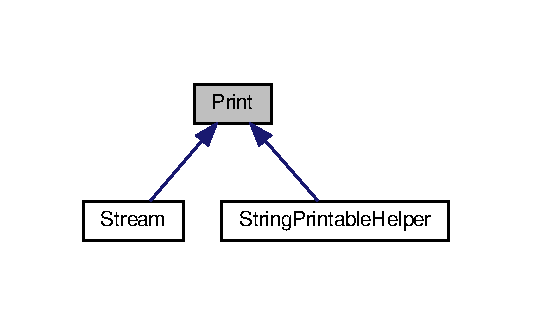
\includegraphics[width=256pt]{class_print__inherit__graph}
\end{center}
\end{figure}
\subsection*{Public Member Functions}
\begin{DoxyCompactItemize}
\item 
\textbf{ Print} ()
\item 
virtual \textbf{ $\sim$\+Print} ()
\item 
int \textbf{ get\+Write\+Error} ()
\item 
void \textbf{ clear\+Write\+Error} ()
\item 
virtual size\+\_\+t \textbf{ write} (uint8\+\_\+t)=0
\item 
size\+\_\+t \textbf{ write} (const char $\ast$str)
\item 
virtual size\+\_\+t \textbf{ write} (const uint8\+\_\+t $\ast$buffer, size\+\_\+t size)
\item 
size\+\_\+t \textbf{ print} (const char[$\,$])
\item 
size\+\_\+t \textbf{ print} (char)
\item 
size\+\_\+t \textbf{ print} (unsigned char, int=\textbf{ D\+EC})
\item 
size\+\_\+t \textbf{ print} (int, int=\textbf{ D\+EC})
\item 
size\+\_\+t \textbf{ print} (unsigned int, int=\textbf{ D\+EC})
\item 
size\+\_\+t \textbf{ print} (long, int=\textbf{ D\+EC})
\item 
size\+\_\+t \textbf{ print} (unsigned long, int=\textbf{ D\+EC})
\item 
size\+\_\+t \textbf{ print} (double, int=2)
\item 
size\+\_\+t \textbf{ print} (const \textbf{ Printable} \&)
\item 
size\+\_\+t \textbf{ println} (const char[$\,$])
\item 
size\+\_\+t \textbf{ println} (char)
\item 
size\+\_\+t \textbf{ println} (unsigned char, int=\textbf{ D\+EC})
\item 
size\+\_\+t \textbf{ println} (int, int=\textbf{ D\+EC})
\item 
size\+\_\+t \textbf{ println} (unsigned int, int=\textbf{ D\+EC})
\item 
size\+\_\+t \textbf{ println} (long, int=\textbf{ D\+EC})
\item 
size\+\_\+t \textbf{ println} (unsigned long, int=\textbf{ D\+EC})
\item 
size\+\_\+t \textbf{ println} (double, int=2)
\item 
size\+\_\+t \textbf{ println} (const \textbf{ Printable} \&)
\item 
size\+\_\+t \textbf{ println} (void)
\item 
{\footnotesize template$<$typename... Args$>$ }\\size\+\_\+t \textbf{ printf} (const char $\ast$format, Args... args)
\item 
{\footnotesize template$<$typename... Args$>$ }\\size\+\_\+t \textbf{ printlnf} (const char $\ast$format, Args... args)
\item 
\textbf{ Print} ()
\item 
virtual \textbf{ $\sim$\+Print} ()
\item 
int \textbf{ get\+Write\+Error} ()
\begin{DoxyCompactList}\small\item\em Return the last error code. 0 means no error. \end{DoxyCompactList}\item 
void \textbf{ clear\+Write\+Error} ()
\begin{DoxyCompactList}\small\item\em Clear the last error code to 0. \end{DoxyCompactList}\item 
virtual size\+\_\+t \textbf{ write} (uint8\+\_\+t c)=0
\begin{DoxyCompactList}\small\item\em Write a single byte to the stream or file. \end{DoxyCompactList}\item 
size\+\_\+t \textbf{ write} (const char $\ast$str)
\begin{DoxyCompactList}\small\item\em Write a null-\/terminated c-\/string the stream or file. \end{DoxyCompactList}\item 
virtual size\+\_\+t \textbf{ write} (const uint8\+\_\+t $\ast$buffer, size\+\_\+t size)
\begin{DoxyCompactList}\small\item\em Write a bytes specified by a buffer and length to the stream or file. \end{DoxyCompactList}\item 
size\+\_\+t \textbf{ print} (const char[$\,$])
\begin{DoxyCompactList}\small\item\em \doxyref{Print}{p.}{class_print} a null-\/terminated array of char variables (a c-\/string) to the stream or file. \end{DoxyCompactList}\item 
size\+\_\+t \textbf{ print} (char)
\begin{DoxyCompactList}\small\item\em \doxyref{Print}{p.}{class_print} a single character to the stream or file. \end{DoxyCompactList}\item 
size\+\_\+t \textbf{ print} (unsigned char value, int base=\textbf{ D\+EC})
\begin{DoxyCompactList}\small\item\em \doxyref{Print}{p.}{class_print} an unsigned char (byte value, 8 bits) in the specified base to the stream or file. \end{DoxyCompactList}\item 
size\+\_\+t \textbf{ print} (int value, int base=\textbf{ D\+EC})
\begin{DoxyCompactList}\small\item\em \doxyref{Print}{p.}{class_print} an int (32 bit integer) the specified base to the stream or file. \end{DoxyCompactList}\item 
size\+\_\+t \textbf{ print} (unsigned int value, int base=\textbf{ D\+EC})
\begin{DoxyCompactList}\small\item\em \doxyref{Print}{p.}{class_print} an unsigned int (32 bit unsigned integer) the specified base to the stream or file. \end{DoxyCompactList}\item 
size\+\_\+t \textbf{ print} (long value, int base=\textbf{ D\+EC})
\begin{DoxyCompactList}\small\item\em \doxyref{Print}{p.}{class_print} a long (32 bit integer) the specified base to the stream or file. \end{DoxyCompactList}\item 
size\+\_\+t \textbf{ print} (unsigned long value, int base=\textbf{ D\+EC})
\begin{DoxyCompactList}\small\item\em \doxyref{Print}{p.}{class_print} a unsigned long (32 bit unsigned integer) the specified base to the stream or file. \end{DoxyCompactList}\item 
size\+\_\+t \textbf{ print} (double value, int dec=2)
\begin{DoxyCompactList}\small\item\em \doxyref{Print}{p.}{class_print} a double floating point value to the stream or file. \end{DoxyCompactList}\item 
size\+\_\+t \textbf{ print} (const \textbf{ Printable} \&)
\begin{DoxyCompactList}\small\item\em \doxyref{Print}{p.}{class_print} an object derived from \doxyref{Printable}{p.}{class_printable} to the stream or file. \end{DoxyCompactList}\item 
size\+\_\+t \textbf{ print} (const \+\_\+\+\_\+\+Flash\+String\+Helper $\ast$)
\item 
size\+\_\+t \textbf{ println} (const char[$\,$])
\begin{DoxyCompactList}\small\item\em \doxyref{Print}{p.}{class_print} a null-\/terminated array of char variables (a c-\/string) plus a C\+R\+LF end-\/of-\/line terminator to the stream or file. \end{DoxyCompactList}\item 
size\+\_\+t \textbf{ println} (char value)
\begin{DoxyCompactList}\small\item\em \doxyref{Print}{p.}{class_print} a single character plus a C\+R\+LF end-\/of-\/line terminator to the stream or file. \end{DoxyCompactList}\item 
size\+\_\+t \textbf{ println} (unsigned char value, int base=\textbf{ D\+EC})
\begin{DoxyCompactList}\small\item\em \doxyref{Print}{p.}{class_print} an unsigned char (byte value. 8 bits) in the specified base plus a C\+R\+LF end-\/of-\/line terminator to the stream or file. \end{DoxyCompactList}\item 
size\+\_\+t \textbf{ println} (int value, int base=\textbf{ D\+EC})
\begin{DoxyCompactList}\small\item\em \doxyref{Print}{p.}{class_print} an int (32 bit integer) the specified base to plus a C\+R\+LF end-\/of-\/line terminator the stream or file. \end{DoxyCompactList}\item 
size\+\_\+t \textbf{ println} (unsigned int value, int base=\textbf{ D\+EC})
\begin{DoxyCompactList}\small\item\em \doxyref{Print}{p.}{class_print} an unsigned int (32 bit unsigned integer) the specified base plus a C\+R\+LF end-\/of-\/line terminator to the stream or file. \end{DoxyCompactList}\item 
size\+\_\+t \textbf{ println} (long value, int base=\textbf{ D\+EC})
\begin{DoxyCompactList}\small\item\em \doxyref{Print}{p.}{class_print} a long (32 bit signed integer) the specified base plus a C\+R\+LF end-\/of-\/line terminator to the stream or file. \end{DoxyCompactList}\item 
size\+\_\+t \textbf{ println} (unsigned long value, int base=\textbf{ D\+EC})
\begin{DoxyCompactList}\small\item\em \doxyref{Print}{p.}{class_print} a unsigned long (32 bit unsigned integer) the specified base plus a C\+R\+LF end-\/of-\/line terminator to the stream or file. \end{DoxyCompactList}\item 
size\+\_\+t \textbf{ println} (double value, int dec=2)
\begin{DoxyCompactList}\small\item\em \doxyref{Print}{p.}{class_print} a double floating point value plus a C\+R\+LF end-\/of-\/line terminator to the stream or file. \end{DoxyCompactList}\item 
size\+\_\+t \textbf{ println} (const \textbf{ Printable} \&)
\begin{DoxyCompactList}\small\item\em \doxyref{Print}{p.}{class_print} an object derived from \doxyref{Printable}{p.}{class_printable} plus a C\+R\+LF end-\/of-\/line terminator to the stream or file. \end{DoxyCompactList}\item 
size\+\_\+t \textbf{ println} (void)
\begin{DoxyCompactList}\small\item\em \doxyref{Print}{p.}{class_print} a C\+R\+LF end-\/of-\/line terminator to the stream or file. \end{DoxyCompactList}\item 
size\+\_\+t \textbf{ println} (const \+\_\+\+\_\+\+Flash\+String\+Helper $\ast$)
\item 
{\footnotesize template$<$typename... Args$>$ }\\size\+\_\+t \textbf{ printf} (const char $\ast$format, Args... args)
\begin{DoxyCompactList}\small\item\em \doxyref{Print}{p.}{class_print} using printf-\/style formatting to the stream or file. \end{DoxyCompactList}\item 
{\footnotesize template$<$typename... Args$>$ }\\size\+\_\+t \textbf{ printlnf} (const char $\ast$format, Args... args)
\begin{DoxyCompactList}\small\item\em \doxyref{Print}{p.}{class_print} using printf-\/style formatting plus a C\+R\+LF end-\/of-\/line terminator to the stream or file. \end{DoxyCompactList}\end{DoxyCompactItemize}
\subsection*{Protected Member Functions}
\begin{DoxyCompactItemize}
\item 
void \textbf{ set\+Write\+Error} (int err=1)
\item 
size\+\_\+t \textbf{ printf\+\_\+impl} (bool newline, const char $\ast$format,...)
\item 
void \textbf{ set\+Write\+Error} (int err=1)
\item 
size\+\_\+t \textbf{ printf\+\_\+impl} (bool newline, const char $\ast$format,...)
\end{DoxyCompactItemize}
\subsection*{Private Member Functions}
\begin{DoxyCompactItemize}
\item 
size\+\_\+t \textbf{ print\+Number} (unsigned long, uint8\+\_\+t)
\item 
size\+\_\+t \textbf{ print\+Float} (double, uint8\+\_\+t)
\item 
size\+\_\+t \textbf{ print\+Number} (unsigned long, uint8\+\_\+t)
\item 
size\+\_\+t \textbf{ print\+Float} (double, uint8\+\_\+t)
\end{DoxyCompactItemize}
\subsection*{Private Attributes}
\begin{DoxyCompactItemize}
\item 
int \textbf{ write\+\_\+error}
\end{DoxyCompactItemize}


\subsection{Detailed Description}
Class for printing to a stream or file. 

Various classes include serial, T\+CP network streams, and files inherit from this and can use these methods. 

Definition at line 44 of file spark\+\_\+wiring\+\_\+print.\+h.



\subsection{Constructor \& Destructor Documentation}
\mbox{\label{class_print_a1b9fe938883bb7b4bce8fba012dab112}} 
\index{Print@{Print}!Print@{Print}}
\index{Print@{Print}!Print@{Print}}
\subsubsection{Print()\hspace{0.1cm}{\footnotesize\ttfamily [1/2]}}
{\footnotesize\ttfamily Print\+::\+Print (\begin{DoxyParamCaption}{ }\end{DoxyParamCaption})\hspace{0.3cm}{\ttfamily [inline]}}



Definition at line 55 of file spark\+\_\+wiring\+\_\+print.\+h.



References write\+\_\+error.


\begin{DoxyCode}
55 : write_error(0) \{\}
\end{DoxyCode}
\mbox{\label{class_print_abc6ea5fd3d477d9465a57421ccd00ba4}} 
\index{Print@{Print}!````~Print@{$\sim$\+Print}}
\index{````~Print@{$\sim$\+Print}!Print@{Print}}
\subsubsection{$\sim$\+Print()\hspace{0.1cm}{\footnotesize\ttfamily [1/2]}}
{\footnotesize\ttfamily virtual Print\+::$\sim$\+Print (\begin{DoxyParamCaption}{ }\end{DoxyParamCaption})\hspace{0.3cm}{\ttfamily [inline]}, {\ttfamily [virtual]}}



Definition at line 56 of file spark\+\_\+wiring\+\_\+print.\+h.


\begin{DoxyCode}
56 \{\}
\end{DoxyCode}
\mbox{\label{class_print_a1b9fe938883bb7b4bce8fba012dab112}} 
\index{Print@{Print}!Print@{Print}}
\index{Print@{Print}!Print@{Print}}
\subsubsection{Print()\hspace{0.1cm}{\footnotesize\ttfamily [2/2]}}
{\footnotesize\ttfamily Print\+::\+Print (\begin{DoxyParamCaption}{ }\end{DoxyParamCaption})\hspace{0.3cm}{\ttfamily [inline]}}



Definition at line 64 of file spark\+\_\+wiring\+\_\+print.\+h.


\begin{DoxyCode}
64 : write_error(0) \{\}
\end{DoxyCode}
\mbox{\label{class_print_abc6ea5fd3d477d9465a57421ccd00ba4}} 
\index{Print@{Print}!````~Print@{$\sim$\+Print}}
\index{````~Print@{$\sim$\+Print}!Print@{Print}}
\subsubsection{$\sim$\+Print()\hspace{0.1cm}{\footnotesize\ttfamily [2/2]}}
{\footnotesize\ttfamily virtual Print\+::$\sim$\+Print (\begin{DoxyParamCaption}{ }\end{DoxyParamCaption})\hspace{0.3cm}{\ttfamily [inline]}, {\ttfamily [virtual]}}



Definition at line 66 of file spark\+\_\+wiring\+\_\+print.\+h.


\begin{DoxyCode}
66 \{\}
\end{DoxyCode}


\subsection{Member Function Documentation}
\mbox{\label{class_print_aec9ecf84cc6d9087a650def3cefc459e}} 
\index{Print@{Print}!clear\+Write\+Error@{clear\+Write\+Error}}
\index{clear\+Write\+Error@{clear\+Write\+Error}!Print@{Print}}
\subsubsection{clear\+Write\+Error()\hspace{0.1cm}{\footnotesize\ttfamily [1/2]}}
{\footnotesize\ttfamily void Print\+::clear\+Write\+Error (\begin{DoxyParamCaption}{ }\end{DoxyParamCaption})\hspace{0.3cm}{\ttfamily [inline]}}



Definition at line 59 of file spark\+\_\+wiring\+\_\+print.\+h.



References set\+Write\+Error().


\begin{DoxyCode}
59 \{ setWriteError(0); \}
\end{DoxyCode}
\mbox{\label{class_print_aec9ecf84cc6d9087a650def3cefc459e}} 
\index{Print@{Print}!clear\+Write\+Error@{clear\+Write\+Error}}
\index{clear\+Write\+Error@{clear\+Write\+Error}!Print@{Print}}
\subsubsection{clear\+Write\+Error()\hspace{0.1cm}{\footnotesize\ttfamily [2/2]}}
{\footnotesize\ttfamily void Print\+::clear\+Write\+Error (\begin{DoxyParamCaption}{ }\end{DoxyParamCaption})\hspace{0.3cm}{\ttfamily [inline]}}



Clear the last error code to 0. 



Definition at line 76 of file spark\+\_\+wiring\+\_\+print.\+h.


\begin{DoxyCode}
76 \{ setWriteError(0); \}
\end{DoxyCode}
\mbox{\label{class_print_a88a4a829fb5d589efb43955ad0cbddcc}} 
\index{Print@{Print}!get\+Write\+Error@{get\+Write\+Error}}
\index{get\+Write\+Error@{get\+Write\+Error}!Print@{Print}}
\subsubsection{get\+Write\+Error()\hspace{0.1cm}{\footnotesize\ttfamily [1/2]}}
{\footnotesize\ttfamily int Print\+::get\+Write\+Error (\begin{DoxyParamCaption}{ }\end{DoxyParamCaption})\hspace{0.3cm}{\ttfamily [inline]}}



Definition at line 58 of file spark\+\_\+wiring\+\_\+print.\+h.



References write\+\_\+error.


\begin{DoxyCode}
58 \{ \textcolor{keywordflow}{return} write_error; \}
\end{DoxyCode}
\mbox{\label{class_print_a88a4a829fb5d589efb43955ad0cbddcc}} 
\index{Print@{Print}!get\+Write\+Error@{get\+Write\+Error}}
\index{get\+Write\+Error@{get\+Write\+Error}!Print@{Print}}
\subsubsection{get\+Write\+Error()\hspace{0.1cm}{\footnotesize\ttfamily [2/2]}}
{\footnotesize\ttfamily int Print\+::get\+Write\+Error (\begin{DoxyParamCaption}{ }\end{DoxyParamCaption})\hspace{0.3cm}{\ttfamily [inline]}}



Return the last error code. 0 means no error. 



Definition at line 71 of file spark\+\_\+wiring\+\_\+print.\+h.


\begin{DoxyCode}
71 \{ \textcolor{keywordflow}{return} write_error; \}
\end{DoxyCode}
\mbox{\label{class_print_acfe80773011eb17dfb52c2fba517a093}} 
\index{Print@{Print}!print@{print}}
\index{print@{print}!Print@{Print}}
\subsubsection{print()\hspace{0.1cm}{\footnotesize\ttfamily [1/19]}}
{\footnotesize\ttfamily size\+\_\+t Print\+::print (\begin{DoxyParamCaption}\item[{const char}]{str[$\,$] }\end{DoxyParamCaption})}



Definition at line 53 of file spark\+\_\+wiring\+\_\+print.\+cpp.



References write().



Referenced by printf\+\_\+impl(), print\+Float(), and println().


\begin{DoxyCode}
54 \{
55   \textcolor{keywordflow}{return} write(str);
56 \}
\end{DoxyCode}
\mbox{\label{class_print_a1e411d07a8ffec5faf7ce485bac0f029}} 
\index{Print@{Print}!print@{print}}
\index{print@{print}!Print@{Print}}
\subsubsection{print()\hspace{0.1cm}{\footnotesize\ttfamily [2/19]}}
{\footnotesize\ttfamily size\+\_\+t Print\+::print (\begin{DoxyParamCaption}\item[{char}]{c }\end{DoxyParamCaption})}



Definition at line 58 of file spark\+\_\+wiring\+\_\+print.\+cpp.



References write().



Referenced by print(), print\+Float(), and println().


\begin{DoxyCode}
59 \{
60   \textcolor{keywordflow}{return} write(c);
61 \}
\end{DoxyCode}
\mbox{\label{class_print_a97bd44df9222fa4a51a1266fab8d3bc1}} 
\index{Print@{Print}!print@{print}}
\index{print@{print}!Print@{Print}}
\subsubsection{print()\hspace{0.1cm}{\footnotesize\ttfamily [3/19]}}
{\footnotesize\ttfamily size\+\_\+t Print\+::print (\begin{DoxyParamCaption}\item[{unsigned char}]{b,  }\item[{int}]{base = {\ttfamily \textbf{ D\+EC}} }\end{DoxyParamCaption})}



Definition at line 63 of file spark\+\_\+wiring\+\_\+print.\+cpp.



References print().



Referenced by println().


\begin{DoxyCode}
64 \{
65   \textcolor{keywordflow}{return} print((\textcolor{keywordtype}{unsigned} \textcolor{keywordtype}{long}) b, base);
66 \}
\end{DoxyCode}
\mbox{\label{class_print_a32cb3cf32d701c797b2b2d1080052dfe}} 
\index{Print@{Print}!print@{print}}
\index{print@{print}!Print@{Print}}
\subsubsection{print()\hspace{0.1cm}{\footnotesize\ttfamily [4/19]}}
{\footnotesize\ttfamily size\+\_\+t Print\+::print (\begin{DoxyParamCaption}\item[{int}]{n,  }\item[{int}]{base = {\ttfamily \textbf{ D\+EC}} }\end{DoxyParamCaption})}



Definition at line 68 of file spark\+\_\+wiring\+\_\+print.\+cpp.



References print().



Referenced by print\+Float(), and println().


\begin{DoxyCode}
69 \{
70   \textcolor{keywordflow}{return} print((\textcolor{keywordtype}{long}) n, base);
71 \}
\end{DoxyCode}
\mbox{\label{class_print_a87275de35583868a370f43ce1c887750}} 
\index{Print@{Print}!print@{print}}
\index{print@{print}!Print@{Print}}
\subsubsection{print()\hspace{0.1cm}{\footnotesize\ttfamily [5/19]}}
{\footnotesize\ttfamily size\+\_\+t Print\+::print (\begin{DoxyParamCaption}\item[{unsigned int}]{n,  }\item[{int}]{base = {\ttfamily \textbf{ D\+EC}} }\end{DoxyParamCaption})}



Definition at line 73 of file spark\+\_\+wiring\+\_\+print.\+cpp.



References print().



Referenced by println().


\begin{DoxyCode}
74 \{
75   \textcolor{keywordflow}{return} print((\textcolor{keywordtype}{unsigned} \textcolor{keywordtype}{long}) n, base);
76 \}
\end{DoxyCode}
\mbox{\label{class_print_ab1fb2a2384c7b9f628943f5046e7d1c1}} 
\index{Print@{Print}!print@{print}}
\index{print@{print}!Print@{Print}}
\subsubsection{print()\hspace{0.1cm}{\footnotesize\ttfamily [6/19]}}
{\footnotesize\ttfamily size\+\_\+t Print\+::print (\begin{DoxyParamCaption}\item[{long}]{n,  }\item[{int}]{base = {\ttfamily \textbf{ D\+EC}} }\end{DoxyParamCaption})}



Definition at line 78 of file spark\+\_\+wiring\+\_\+print.\+cpp.



References print(), print\+Number(), and write().



Referenced by print(), and println().


\begin{DoxyCode}
79 \{
80   \textcolor{keywordflow}{if} (base == 0) \{
81     \textcolor{keywordflow}{return} write(n);
82   \} \textcolor{keywordflow}{else} \textcolor{keywordflow}{if} (base == 10) \{
83     \textcolor{keywordflow}{if} (n < 0) \{
84       \textcolor{keywordtype}{int} t = print(\textcolor{charliteral}{'-'});
85       n = -n;
86       \textcolor{keywordflow}{return} printNumber(n, 10) + t;
87     \}
88     \textcolor{keywordflow}{return} printNumber(n, 10);
89   \} \textcolor{keywordflow}{else} \{
90     \textcolor{keywordflow}{return} printNumber(n, base);
91   \}
92 \}
\end{DoxyCode}
\mbox{\label{class_print_a26a40be7a557c0bc391a15dce9f06954}} 
\index{Print@{Print}!print@{print}}
\index{print@{print}!Print@{Print}}
\subsubsection{print()\hspace{0.1cm}{\footnotesize\ttfamily [7/19]}}
{\footnotesize\ttfamily size\+\_\+t Print\+::print (\begin{DoxyParamCaption}\item[{unsigned long}]{n,  }\item[{int}]{base = {\ttfamily \textbf{ D\+EC}} }\end{DoxyParamCaption})}



Definition at line 94 of file spark\+\_\+wiring\+\_\+print.\+cpp.



References print\+Number(), and write().



Referenced by print(), print\+Float(), and println().


\begin{DoxyCode}
95 \{
96   \textcolor{keywordflow}{if} (base == 0) \textcolor{keywordflow}{return} write(n);
97   \textcolor{keywordflow}{else} \textcolor{keywordflow}{return} printNumber(n, base);
98 \}
\end{DoxyCode}
\mbox{\label{class_print_ae8b4c025786c820afe0a90aeea01c9c5}} 
\index{Print@{Print}!print@{print}}
\index{print@{print}!Print@{Print}}
\subsubsection{print()\hspace{0.1cm}{\footnotesize\ttfamily [8/19]}}
{\footnotesize\ttfamily size\+\_\+t Print\+::print (\begin{DoxyParamCaption}\item[{double}]{n,  }\item[{int}]{digits = {\ttfamily 2} }\end{DoxyParamCaption})}



Definition at line 100 of file spark\+\_\+wiring\+\_\+print.\+cpp.



References print\+Float().



Referenced by println().


\begin{DoxyCode}
101 \{
102   \textcolor{keywordflow}{return} printFloat(n, digits);
103 \}
\end{DoxyCode}
\mbox{\label{class_print_a901b0f06ae34aab31b8fbb4298f0596e}} 
\index{Print@{Print}!print@{print}}
\index{print@{print}!Print@{Print}}
\subsubsection{print()\hspace{0.1cm}{\footnotesize\ttfamily [9/19]}}
{\footnotesize\ttfamily size\+\_\+t Print\+::print (\begin{DoxyParamCaption}\item[{const \textbf{ Printable} \&}]{x }\end{DoxyParamCaption})}



Definition at line 105 of file spark\+\_\+wiring\+\_\+print.\+cpp.



References Printable\+::print\+To().



Referenced by println().


\begin{DoxyCode}
106  \{
107    \textcolor{keywordflow}{return} x.printTo(*\textcolor{keyword}{this});
108  \}
\end{DoxyCode}
\mbox{\label{class_print_acfe80773011eb17dfb52c2fba517a093}} 
\index{Print@{Print}!print@{print}}
\index{print@{print}!Print@{Print}}
\subsubsection{print()\hspace{0.1cm}{\footnotesize\ttfamily [10/19]}}
{\footnotesize\ttfamily size\+\_\+t Print\+::print (\begin{DoxyParamCaption}\item[{const char}]{[$\,$] }\end{DoxyParamCaption})}



\doxyref{Print}{p.}{class_print} a null-\/terminated array of char variables (a c-\/string) to the stream or file. 

\mbox{\label{class_print_a1e411d07a8ffec5faf7ce485bac0f029}} 
\index{Print@{Print}!print@{print}}
\index{print@{print}!Print@{Print}}
\subsubsection{print()\hspace{0.1cm}{\footnotesize\ttfamily [11/19]}}
{\footnotesize\ttfamily size\+\_\+t Print\+::print (\begin{DoxyParamCaption}\item[{char}]{ }\end{DoxyParamCaption})}



\doxyref{Print}{p.}{class_print} a single character to the stream or file. 

\mbox{\label{class_print_ae35481e77567618140cd58d8b96d3747}} 
\index{Print@{Print}!print@{print}}
\index{print@{print}!Print@{Print}}
\subsubsection{print()\hspace{0.1cm}{\footnotesize\ttfamily [12/19]}}
{\footnotesize\ttfamily size\+\_\+t Print\+::print (\begin{DoxyParamCaption}\item[{unsigned char}]{value,  }\item[{int}]{base = {\ttfamily \textbf{ D\+EC}} }\end{DoxyParamCaption})}



\doxyref{Print}{p.}{class_print} an unsigned char (byte value, 8 bits) in the specified base to the stream or file. 


\begin{DoxyParams}{Parameters}
{\em value} & The value to print. \\
\hline
{\em base} & The base to print. Default is D\+EC (decimal). Other values are H\+EX (hexadecimal), O\+CT (octal), and B\+IN (binary). \\
\hline
\end{DoxyParams}
\mbox{\label{class_print_aa28ddbde83b14df73b41c919ecc4478f}} 
\index{Print@{Print}!print@{print}}
\index{print@{print}!Print@{Print}}
\subsubsection{print()\hspace{0.1cm}{\footnotesize\ttfamily [13/19]}}
{\footnotesize\ttfamily size\+\_\+t Print\+::print (\begin{DoxyParamCaption}\item[{int}]{value,  }\item[{int}]{base = {\ttfamily \textbf{ D\+EC}} }\end{DoxyParamCaption})}



\doxyref{Print}{p.}{class_print} an int (32 bit integer) the specified base to the stream or file. 


\begin{DoxyParams}{Parameters}
{\em value} & The value to print. \\
\hline
{\em base} & The base to print. Default is D\+EC (decimal). Other values are H\+EX (hexadecimal), O\+CT (octal), and B\+IN (binary). \\
\hline
\end{DoxyParams}
\mbox{\label{class_print_afcd7d3a184df961a502643e4fb638c52}} 
\index{Print@{Print}!print@{print}}
\index{print@{print}!Print@{Print}}
\subsubsection{print()\hspace{0.1cm}{\footnotesize\ttfamily [14/19]}}
{\footnotesize\ttfamily size\+\_\+t Print\+::print (\begin{DoxyParamCaption}\item[{unsigned int}]{value,  }\item[{int}]{base = {\ttfamily \textbf{ D\+EC}} }\end{DoxyParamCaption})}



\doxyref{Print}{p.}{class_print} an unsigned int (32 bit unsigned integer) the specified base to the stream or file. 


\begin{DoxyParams}{Parameters}
{\em value} & The value to print. \\
\hline
{\em base} & The base to print. Default is D\+EC (decimal). Other values are H\+EX (hexadecimal), O\+CT (octal), and B\+IN (binary). \\
\hline
\end{DoxyParams}
\mbox{\label{class_print_a0c663ac015ebc037ea044ba2e2cf2947}} 
\index{Print@{Print}!print@{print}}
\index{print@{print}!Print@{Print}}
\subsubsection{print()\hspace{0.1cm}{\footnotesize\ttfamily [15/19]}}
{\footnotesize\ttfamily size\+\_\+t Print\+::print (\begin{DoxyParamCaption}\item[{long}]{value,  }\item[{int}]{base = {\ttfamily \textbf{ D\+EC}} }\end{DoxyParamCaption})}



\doxyref{Print}{p.}{class_print} a long (32 bit integer) the specified base to the stream or file. 


\begin{DoxyParams}{Parameters}
{\em value} & The value to print. \\
\hline
{\em base} & The base to print. Default is D\+EC (decimal). Other values are H\+EX (hexadecimal), O\+CT (octal), and B\+IN (binary). \\
\hline
\end{DoxyParams}
\mbox{\label{class_print_acb8c6dcd4339b024436002aa9a6f4be2}} 
\index{Print@{Print}!print@{print}}
\index{print@{print}!Print@{Print}}
\subsubsection{print()\hspace{0.1cm}{\footnotesize\ttfamily [16/19]}}
{\footnotesize\ttfamily size\+\_\+t Print\+::print (\begin{DoxyParamCaption}\item[{unsigned long}]{value,  }\item[{int}]{base = {\ttfamily \textbf{ D\+EC}} }\end{DoxyParamCaption})}



\doxyref{Print}{p.}{class_print} a unsigned long (32 bit unsigned integer) the specified base to the stream or file. 


\begin{DoxyParams}{Parameters}
{\em value} & The value to print. \\
\hline
{\em base} & The base to print. Default is D\+EC (decimal). Other values are H\+EX (hexadecimal), O\+CT (octal), and B\+IN (binary). \\
\hline
\end{DoxyParams}
\mbox{\label{class_print_ad89472bdb6539423a42d350beec02ff4}} 
\index{Print@{Print}!print@{print}}
\index{print@{print}!Print@{Print}}
\subsubsection{print()\hspace{0.1cm}{\footnotesize\ttfamily [17/19]}}
{\footnotesize\ttfamily size\+\_\+t Print\+::print (\begin{DoxyParamCaption}\item[{double}]{value,  }\item[{int}]{dec = {\ttfamily 2} }\end{DoxyParamCaption})}



\doxyref{Print}{p.}{class_print} a double floating point value to the stream or file. 


\begin{DoxyParams}{Parameters}
{\em value} & The value to print. \\
\hline
{\em dec} & The number of decimal places to include for the fractional part. Default\+: 2 \\
\hline
\end{DoxyParams}
\mbox{\label{class_print_a901b0f06ae34aab31b8fbb4298f0596e}} 
\index{Print@{Print}!print@{print}}
\index{print@{print}!Print@{Print}}
\subsubsection{print()\hspace{0.1cm}{\footnotesize\ttfamily [18/19]}}
{\footnotesize\ttfamily size\+\_\+t Print\+::print (\begin{DoxyParamCaption}\item[{const \textbf{ Printable} \&}]{ }\end{DoxyParamCaption})}



\doxyref{Print}{p.}{class_print} an object derived from \doxyref{Printable}{p.}{class_printable} to the stream or file. 

\mbox{\label{class_print_aa4158dd94bc1741f92d99c427261d7c0}} 
\index{Print@{Print}!print@{print}}
\index{print@{print}!Print@{Print}}
\subsubsection{print()\hspace{0.1cm}{\footnotesize\ttfamily [19/19]}}
{\footnotesize\ttfamily size\+\_\+t Print\+::print (\begin{DoxyParamCaption}\item[{const \+\_\+\+\_\+\+Flash\+String\+Helper $\ast$}]{ }\end{DoxyParamCaption})}

\mbox{\label{class_print_a08a461c9fee5fd8f5795d6e9f61e3d5b}} 
\index{Print@{Print}!printf@{printf}}
\index{printf@{printf}!Print@{Print}}
\subsubsection{printf()\hspace{0.1cm}{\footnotesize\ttfamily [1/2]}}
{\footnotesize\ttfamily template$<$typename... Args$>$ \\
size\+\_\+t Print\+::printf (\begin{DoxyParamCaption}\item[{const char $\ast$}]{format,  }\item[{Args...}]{args }\end{DoxyParamCaption})\hspace{0.3cm}{\ttfamily [inline]}}



Definition at line 90 of file spark\+\_\+wiring\+\_\+print.\+h.



References printf\+\_\+impl().


\begin{DoxyCode}
91     \{
92         \textcolor{keywordflow}{return} this->printf_impl(\textcolor{keyword}{false}, format, args...);
93     \}
\end{DoxyCode}
\mbox{\label{class_print_a08a461c9fee5fd8f5795d6e9f61e3d5b}} 
\index{Print@{Print}!printf@{printf}}
\index{printf@{printf}!Print@{Print}}
\subsubsection{printf()\hspace{0.1cm}{\footnotesize\ttfamily [2/2]}}
{\footnotesize\ttfamily template$<$typename... Args$>$ \\
size\+\_\+t Print\+::printf (\begin{DoxyParamCaption}\item[{const char $\ast$}]{format,  }\item[{Args...}]{args }\end{DoxyParamCaption})\hspace{0.3cm}{\ttfamily [inline]}}



\doxyref{Print}{p.}{class_print} using printf-\/style formatting to the stream or file. 


\begin{DoxyParams}{Parameters}
{\em format} & printf-\/style formatting string\\
\hline
{\em args} & variable arguments \\
\hline
\end{DoxyParams}


Definition at line 256 of file spark\+\_\+wiring\+\_\+print.\+h.


\begin{DoxyCode}
257     \{
258         \textcolor{keywordflow}{return} this->printf_impl(\textcolor{keyword}{false}, format, args...);
259     \}
\end{DoxyCode}
\mbox{\label{class_print_af887fd768601c2ee2b18d1deb20b151d}} 
\index{Print@{Print}!printf\+\_\+impl@{printf\+\_\+impl}}
\index{printf\+\_\+impl@{printf\+\_\+impl}!Print@{Print}}
\subsubsection{printf\+\_\+impl()\hspace{0.1cm}{\footnotesize\ttfamily [1/2]}}
{\footnotesize\ttfamily size\+\_\+t Print\+::printf\+\_\+impl (\begin{DoxyParamCaption}\item[{bool}]{newline,  }\item[{const char $\ast$}]{format,  }\item[{}]{... }\end{DoxyParamCaption})\hspace{0.3cm}{\ttfamily [protected]}}



Definition at line 246 of file spark\+\_\+wiring\+\_\+print.\+cpp.



References print(), and println().



Referenced by printf(), and printlnf().


\begin{DoxyCode}
247 \{
248     \textcolor{keyword}{const} \textcolor{keywordtype}{int} bufsize = 20;
249     \textcolor{keywordtype}{char} test[bufsize];
250     va\_list marker;
251     va\_start(marker, format);
252     \textcolor{keywordtype}{size\_t} n = vsnprintf(test, bufsize, format, marker);
253     va\_end(marker);
254 
255     \textcolor{keywordflow}{if} (n<bufsize)
256     \{
257         n = print(test);
258     \}
259     \textcolor{keywordflow}{else}
260     \{
261         \textcolor{keywordtype}{char} bigger[n+1];
262         va\_start(marker, format);
263         n = vsnprintf(bigger, n+1, format, marker);
264         va\_end(marker);
265         n = print(bigger);
266     \}
267     \textcolor{keywordflow}{if} (newline)
268         n += println();
269     \textcolor{keywordflow}{return} n;
270 \}
\end{DoxyCode}
\mbox{\label{class_print_af887fd768601c2ee2b18d1deb20b151d}} 
\index{Print@{Print}!printf\+\_\+impl@{printf\+\_\+impl}}
\index{printf\+\_\+impl@{printf\+\_\+impl}!Print@{Print}}
\subsubsection{printf\+\_\+impl()\hspace{0.1cm}{\footnotesize\ttfamily [2/2]}}
{\footnotesize\ttfamily size\+\_\+t Print\+::printf\+\_\+impl (\begin{DoxyParamCaption}\item[{bool}]{newline,  }\item[{const char $\ast$}]{format,  }\item[{}]{... }\end{DoxyParamCaption})\hspace{0.3cm}{\ttfamily [protected]}}

\mbox{\label{class_print_a449fd5f2ab1fb43c3e3b10f53d18b1e8}} 
\index{Print@{Print}!print\+Float@{print\+Float}}
\index{print\+Float@{print\+Float}!Print@{Print}}
\subsubsection{print\+Float()\hspace{0.1cm}{\footnotesize\ttfamily [1/2]}}
{\footnotesize\ttfamily size\+\_\+t Print\+::print\+Float (\begin{DoxyParamCaption}\item[{double}]{number,  }\item[{uint8\+\_\+t}]{digits }\end{DoxyParamCaption})\hspace{0.3cm}{\ttfamily [private]}}



Definition at line 201 of file spark\+\_\+wiring\+\_\+print.\+cpp.



References print().



Referenced by print().


\begin{DoxyCode}
202 \{
203   \textcolor{keywordtype}{size\_t} n = 0;
204 
205   \textcolor{keywordflow}{if} (isnan(number)) \textcolor{keywordflow}{return} print(\textcolor{stringliteral}{"nan"});
206   \textcolor{keywordflow}{if} (isinf(number)) \textcolor{keywordflow}{return} print(\textcolor{stringliteral}{"inf"});
207   \textcolor{keywordflow}{if} (number > 4294967040.0) \textcolor{keywordflow}{return} print (\textcolor{stringliteral}{"ovf"});  \textcolor{comment}{// constant determined empirically}
208   \textcolor{keywordflow}{if} (number <-4294967040.0) \textcolor{keywordflow}{return} print (\textcolor{stringliteral}{"ovf"});  \textcolor{comment}{// constant determined empirically}
209 
210   \textcolor{comment}{// Handle negative numbers}
211   \textcolor{keywordflow}{if} (number < 0.0)
212   \{
213      n += print(\textcolor{charliteral}{'-'});
214      number = -number;
215   \}
216 
217   \textcolor{comment}{// Round correctly so that print(1.999, 2) prints as "2.00"}
218   \textcolor{keywordtype}{double} rounding = 0.5;
219   \textcolor{keywordflow}{for} (uint8\_t i=0; i<digits; ++i)
220     rounding /= 10.0;
221 
222   number += rounding;
223 
224   \textcolor{comment}{// Extract the integer part of the number and print it}
225   \textcolor{keywordtype}{unsigned} \textcolor{keywordtype}{long} int\_part = (\textcolor{keywordtype}{unsigned} long)number;
226   \textcolor{keywordtype}{double} remainder = number - (double)int\_part;
227   n += print(int\_part);
228 
229   \textcolor{comment}{// Print the decimal point, but only if there are digits beyond}
230   \textcolor{keywordflow}{if} (digits > 0) \{
231     n += print(\textcolor{stringliteral}{"."});
232   \}
233 
234   \textcolor{comment}{// Extract digits from the remainder one at a time}
235   \textcolor{keywordflow}{while} (digits-- > 0)
236   \{
237     remainder *= 10.0;
238     \textcolor{keywordtype}{int} toPrint = int(remainder);
239     n += print(toPrint);
240     remainder -= toPrint;
241   \}
242 
243   \textcolor{keywordflow}{return} n;
244 \}
\end{DoxyCode}
\mbox{\label{class_print_a449fd5f2ab1fb43c3e3b10f53d18b1e8}} 
\index{Print@{Print}!print\+Float@{print\+Float}}
\index{print\+Float@{print\+Float}!Print@{Print}}
\subsubsection{print\+Float()\hspace{0.1cm}{\footnotesize\ttfamily [2/2]}}
{\footnotesize\ttfamily size\+\_\+t Print\+::print\+Float (\begin{DoxyParamCaption}\item[{double}]{,  }\item[{uint8\+\_\+t}]{ }\end{DoxyParamCaption})\hspace{0.3cm}{\ttfamily [private]}}

\mbox{\label{class_print_ad337ce3f7977411b7d34d47a51e5737e}} 
\index{Print@{Print}!println@{println}}
\index{println@{println}!Print@{Print}}
\subsubsection{println()\hspace{0.1cm}{\footnotesize\ttfamily [1/21]}}
{\footnotesize\ttfamily size\+\_\+t Print\+::println (\begin{DoxyParamCaption}\item[{const char}]{c[$\,$] }\end{DoxyParamCaption})}



Definition at line 117 of file spark\+\_\+wiring\+\_\+print.\+cpp.



References print(), and println().


\begin{DoxyCode}
118 \{
119   \textcolor{keywordtype}{size\_t} n = print(c);
120   n += println();
121   \textcolor{keywordflow}{return} n;
122 \}
\end{DoxyCode}
\mbox{\label{class_print_a554896a71162f967b5794401239d7a01}} 
\index{Print@{Print}!println@{println}}
\index{println@{println}!Print@{Print}}
\subsubsection{println()\hspace{0.1cm}{\footnotesize\ttfamily [2/21]}}
{\footnotesize\ttfamily size\+\_\+t Print\+::println (\begin{DoxyParamCaption}\item[{char}]{c }\end{DoxyParamCaption})}



Definition at line 124 of file spark\+\_\+wiring\+\_\+print.\+cpp.



References print(), and println().


\begin{DoxyCode}
125 \{
126   \textcolor{keywordtype}{size\_t} n = print(c);
127   n += println();
128   \textcolor{keywordflow}{return} n;
129 \}
\end{DoxyCode}
\mbox{\label{class_print_ac9afe80f50f0118d735295aec7727e50}} 
\index{Print@{Print}!println@{println}}
\index{println@{println}!Print@{Print}}
\subsubsection{println()\hspace{0.1cm}{\footnotesize\ttfamily [3/21]}}
{\footnotesize\ttfamily size\+\_\+t Print\+::println (\begin{DoxyParamCaption}\item[{unsigned char}]{b,  }\item[{int}]{base = {\ttfamily \textbf{ D\+EC}} }\end{DoxyParamCaption})}



Definition at line 131 of file spark\+\_\+wiring\+\_\+print.\+cpp.



References print(), and println().


\begin{DoxyCode}
132 \{
133   \textcolor{keywordtype}{size\_t} n = print(b, base);
134   n += println();
135   \textcolor{keywordflow}{return} n;
136 \}
\end{DoxyCode}
\mbox{\label{class_print_a738c88471cfb8eac7c8a804699971413}} 
\index{Print@{Print}!println@{println}}
\index{println@{println}!Print@{Print}}
\subsubsection{println()\hspace{0.1cm}{\footnotesize\ttfamily [4/21]}}
{\footnotesize\ttfamily size\+\_\+t Print\+::println (\begin{DoxyParamCaption}\item[{int}]{num,  }\item[{int}]{base = {\ttfamily \textbf{ D\+EC}} }\end{DoxyParamCaption})}



Definition at line 138 of file spark\+\_\+wiring\+\_\+print.\+cpp.



References print(), and println().


\begin{DoxyCode}
139 \{
140   \textcolor{keywordtype}{size\_t} n = print(num, base);
141   n += println();
142   \textcolor{keywordflow}{return} n;
143 \}
\end{DoxyCode}
\mbox{\label{class_print_ac87eed1fcb78641169ba2244278c899e}} 
\index{Print@{Print}!println@{println}}
\index{println@{println}!Print@{Print}}
\subsubsection{println()\hspace{0.1cm}{\footnotesize\ttfamily [5/21]}}
{\footnotesize\ttfamily size\+\_\+t Print\+::println (\begin{DoxyParamCaption}\item[{unsigned int}]{num,  }\item[{int}]{base = {\ttfamily \textbf{ D\+EC}} }\end{DoxyParamCaption})}



Definition at line 145 of file spark\+\_\+wiring\+\_\+print.\+cpp.



References print(), and println().


\begin{DoxyCode}
146 \{
147   \textcolor{keywordtype}{size\_t} n = print(num, base);
148   n += println();
149   \textcolor{keywordflow}{return} n;
150 \}
\end{DoxyCode}
\mbox{\label{class_print_a833fbec3ceba92e3ec95f51e026e4569}} 
\index{Print@{Print}!println@{println}}
\index{println@{println}!Print@{Print}}
\subsubsection{println()\hspace{0.1cm}{\footnotesize\ttfamily [6/21]}}
{\footnotesize\ttfamily size\+\_\+t Print\+::println (\begin{DoxyParamCaption}\item[{long}]{num,  }\item[{int}]{base = {\ttfamily \textbf{ D\+EC}} }\end{DoxyParamCaption})}



Definition at line 152 of file spark\+\_\+wiring\+\_\+print.\+cpp.



References print(), and println().


\begin{DoxyCode}
153 \{
154   \textcolor{keywordtype}{size\_t} n = print(num, base);
155   n += println();
156   \textcolor{keywordflow}{return} n;
157 \}
\end{DoxyCode}
\mbox{\label{class_print_aebee3c33ee5d8f10b6f378d5273742d0}} 
\index{Print@{Print}!println@{println}}
\index{println@{println}!Print@{Print}}
\subsubsection{println()\hspace{0.1cm}{\footnotesize\ttfamily [7/21]}}
{\footnotesize\ttfamily size\+\_\+t Print\+::println (\begin{DoxyParamCaption}\item[{unsigned long}]{num,  }\item[{int}]{base = {\ttfamily \textbf{ D\+EC}} }\end{DoxyParamCaption})}



Definition at line 159 of file spark\+\_\+wiring\+\_\+print.\+cpp.



References print(), and println().


\begin{DoxyCode}
160 \{
161   \textcolor{keywordtype}{size\_t} n = print(num, base);
162   n += println();
163   \textcolor{keywordflow}{return} n;
164 \}
\end{DoxyCode}
\mbox{\label{class_print_a56e976b079361b6021ef7c2bedb397a2}} 
\index{Print@{Print}!println@{println}}
\index{println@{println}!Print@{Print}}
\subsubsection{println()\hspace{0.1cm}{\footnotesize\ttfamily [8/21]}}
{\footnotesize\ttfamily size\+\_\+t Print\+::println (\begin{DoxyParamCaption}\item[{double}]{num,  }\item[{int}]{digits = {\ttfamily 2} }\end{DoxyParamCaption})}



Definition at line 166 of file spark\+\_\+wiring\+\_\+print.\+cpp.



References print(), and println().


\begin{DoxyCode}
167 \{
168   \textcolor{keywordtype}{size\_t} n = print(num, digits);
169   n += println();
170   \textcolor{keywordflow}{return} n;
171 \}
\end{DoxyCode}
\mbox{\label{class_print_a20f9e104153b62e720c9b4c348b44f00}} 
\index{Print@{Print}!println@{println}}
\index{println@{println}!Print@{Print}}
\subsubsection{println()\hspace{0.1cm}{\footnotesize\ttfamily [9/21]}}
{\footnotesize\ttfamily size\+\_\+t Print\+::println (\begin{DoxyParamCaption}\item[{const \textbf{ Printable} \&}]{x }\end{DoxyParamCaption})}



Definition at line 173 of file spark\+\_\+wiring\+\_\+print.\+cpp.



References print(), and println().


\begin{DoxyCode}
174  \{
175    \textcolor{keywordtype}{size\_t} n = print(x);
176    n += println();
177    \textcolor{keywordflow}{return} n;
178  \}
\end{DoxyCode}
\mbox{\label{class_print_a169b128f9e22f0c15883768f580541a2}} 
\index{Print@{Print}!println@{println}}
\index{println@{println}!Print@{Print}}
\subsubsection{println()\hspace{0.1cm}{\footnotesize\ttfamily [10/21]}}
{\footnotesize\ttfamily size\+\_\+t Print\+::println (\begin{DoxyParamCaption}\item[{void}]{ }\end{DoxyParamCaption})}



Definition at line 110 of file spark\+\_\+wiring\+\_\+print.\+cpp.



References print().



Referenced by printf\+\_\+impl(), and println().


\begin{DoxyCode}
111 \{
112   \textcolor{keywordtype}{size\_t} n = print(\textcolor{charliteral}{'\(\backslash\)r'});
113   n += print(\textcolor{charliteral}{'\(\backslash\)n'});
114   \textcolor{keywordflow}{return} n;
115 \}
\end{DoxyCode}
\mbox{\label{class_print_ad337ce3f7977411b7d34d47a51e5737e}} 
\index{Print@{Print}!println@{println}}
\index{println@{println}!Print@{Print}}
\subsubsection{println()\hspace{0.1cm}{\footnotesize\ttfamily [11/21]}}
{\footnotesize\ttfamily size\+\_\+t Print\+::println (\begin{DoxyParamCaption}\item[{const char}]{[$\,$] }\end{DoxyParamCaption})}



\doxyref{Print}{p.}{class_print} a null-\/terminated array of char variables (a c-\/string) plus a C\+R\+LF end-\/of-\/line terminator to the stream or file. 

\mbox{\label{class_print_a80fdd92db4b396062586bcb3e08d3835}} 
\index{Print@{Print}!println@{println}}
\index{println@{println}!Print@{Print}}
\subsubsection{println()\hspace{0.1cm}{\footnotesize\ttfamily [12/21]}}
{\footnotesize\ttfamily size\+\_\+t Print\+::println (\begin{DoxyParamCaption}\item[{char}]{value }\end{DoxyParamCaption})}



\doxyref{Print}{p.}{class_print} a single character plus a C\+R\+LF end-\/of-\/line terminator to the stream or file. 

\mbox{\label{class_print_a000b3fd5b723cb6c7db0d3231a9ef2f8}} 
\index{Print@{Print}!println@{println}}
\index{println@{println}!Print@{Print}}
\subsubsection{println()\hspace{0.1cm}{\footnotesize\ttfamily [13/21]}}
{\footnotesize\ttfamily size\+\_\+t Print\+::println (\begin{DoxyParamCaption}\item[{unsigned char}]{value,  }\item[{int}]{base = {\ttfamily \textbf{ D\+EC}} }\end{DoxyParamCaption})}



\doxyref{Print}{p.}{class_print} an unsigned char (byte value. 8 bits) in the specified base plus a C\+R\+LF end-\/of-\/line terminator to the stream or file. 


\begin{DoxyParams}{Parameters}
{\em value} & The value to print. \\
\hline
{\em base} & The base to print. Default is D\+EC (decimal). Other values are H\+EX (hexadecimal), O\+CT (octal), and B\+IN (binary). \\
\hline
\end{DoxyParams}
\mbox{\label{class_print_a82aa91bbd859f28a0a3b4869e5bfcadd}} 
\index{Print@{Print}!println@{println}}
\index{println@{println}!Print@{Print}}
\subsubsection{println()\hspace{0.1cm}{\footnotesize\ttfamily [14/21]}}
{\footnotesize\ttfamily size\+\_\+t Print\+::println (\begin{DoxyParamCaption}\item[{int}]{value,  }\item[{int}]{base = {\ttfamily \textbf{ D\+EC}} }\end{DoxyParamCaption})}



\doxyref{Print}{p.}{class_print} an int (32 bit integer) the specified base to plus a C\+R\+LF end-\/of-\/line terminator the stream or file. 


\begin{DoxyParams}{Parameters}
{\em value} & The value to print \\
\hline
{\em base} & The base to print. Default is D\+EC (decimal). Other values are H\+EX (hexadecimal), O\+CT (octal), and B\+IN (binary). \\
\hline
\end{DoxyParams}
\mbox{\label{class_print_a2608232c1f10f654111ff447de16d60b}} 
\index{Print@{Print}!println@{println}}
\index{println@{println}!Print@{Print}}
\subsubsection{println()\hspace{0.1cm}{\footnotesize\ttfamily [15/21]}}
{\footnotesize\ttfamily size\+\_\+t Print\+::println (\begin{DoxyParamCaption}\item[{unsigned int}]{value,  }\item[{int}]{base = {\ttfamily \textbf{ D\+EC}} }\end{DoxyParamCaption})}



\doxyref{Print}{p.}{class_print} an unsigned int (32 bit unsigned integer) the specified base plus a C\+R\+LF end-\/of-\/line terminator to the stream or file. 


\begin{DoxyParams}{Parameters}
{\em value} & The value to print \\
\hline
{\em base} & The base to print. Default is D\+EC (decimal). Other values are H\+EX (hexadecimal), O\+CT (octal), and B\+IN (binary). \\
\hline
\end{DoxyParams}
\mbox{\label{class_print_a82bbe59b28440c29e55ff3597eb45376}} 
\index{Print@{Print}!println@{println}}
\index{println@{println}!Print@{Print}}
\subsubsection{println()\hspace{0.1cm}{\footnotesize\ttfamily [16/21]}}
{\footnotesize\ttfamily size\+\_\+t Print\+::println (\begin{DoxyParamCaption}\item[{long}]{value,  }\item[{int}]{base = {\ttfamily \textbf{ D\+EC}} }\end{DoxyParamCaption})}



\doxyref{Print}{p.}{class_print} a long (32 bit signed integer) the specified base plus a C\+R\+LF end-\/of-\/line terminator to the stream or file. 


\begin{DoxyParams}{Parameters}
{\em value} & The value to print \\
\hline
{\em base} & The base to print. Default is D\+EC (decimal). Other values are H\+EX (hexadecimal), O\+CT (octal), and B\+IN (binary). \\
\hline
\end{DoxyParams}
\mbox{\label{class_print_afa936d7e8dd329d9162f2cd28f42681e}} 
\index{Print@{Print}!println@{println}}
\index{println@{println}!Print@{Print}}
\subsubsection{println()\hspace{0.1cm}{\footnotesize\ttfamily [17/21]}}
{\footnotesize\ttfamily size\+\_\+t Print\+::println (\begin{DoxyParamCaption}\item[{unsigned long}]{value,  }\item[{int}]{base = {\ttfamily \textbf{ D\+EC}} }\end{DoxyParamCaption})}



\doxyref{Print}{p.}{class_print} a unsigned long (32 bit unsigned integer) the specified base plus a C\+R\+LF end-\/of-\/line terminator to the stream or file. 


\begin{DoxyParams}{Parameters}
{\em value} & The value to print. \\
\hline
{\em base} & The base to print. Default is D\+EC (decimal). Other values are H\+EX (hexadecimal), O\+CT (octal), and B\+IN (binary). \\
\hline
\end{DoxyParams}
\mbox{\label{class_print_a178b90baf9f74f0945f5c64aafec59ea}} 
\index{Print@{Print}!println@{println}}
\index{println@{println}!Print@{Print}}
\subsubsection{println()\hspace{0.1cm}{\footnotesize\ttfamily [18/21]}}
{\footnotesize\ttfamily size\+\_\+t Print\+::println (\begin{DoxyParamCaption}\item[{double}]{value,  }\item[{int}]{dec = {\ttfamily 2} }\end{DoxyParamCaption})}



\doxyref{Print}{p.}{class_print} a double floating point value plus a C\+R\+LF end-\/of-\/line terminator to the stream or file. 


\begin{DoxyParams}{Parameters}
{\em value} & The value to print. \\
\hline
{\em dec} & The number of decimal places to include for the fractional part. Default\+: 2 \\
\hline
\end{DoxyParams}
\mbox{\label{class_print_a20f9e104153b62e720c9b4c348b44f00}} 
\index{Print@{Print}!println@{println}}
\index{println@{println}!Print@{Print}}
\subsubsection{println()\hspace{0.1cm}{\footnotesize\ttfamily [19/21]}}
{\footnotesize\ttfamily size\+\_\+t Print\+::println (\begin{DoxyParamCaption}\item[{const \textbf{ Printable} \&}]{ }\end{DoxyParamCaption})}



\doxyref{Print}{p.}{class_print} an object derived from \doxyref{Printable}{p.}{class_printable} plus a C\+R\+LF end-\/of-\/line terminator to the stream or file. 

\mbox{\label{class_print_a169b128f9e22f0c15883768f580541a2}} 
\index{Print@{Print}!println@{println}}
\index{println@{println}!Print@{Print}}
\subsubsection{println()\hspace{0.1cm}{\footnotesize\ttfamily [20/21]}}
{\footnotesize\ttfamily size\+\_\+t Print\+::println (\begin{DoxyParamCaption}\item[{void}]{ }\end{DoxyParamCaption})}



\doxyref{Print}{p.}{class_print} a C\+R\+LF end-\/of-\/line terminator to the stream or file. 

\mbox{\label{class_print_a4fd286b325d3b1a786cfa35072a8ef52}} 
\index{Print@{Print}!println@{println}}
\index{println@{println}!Print@{Print}}
\subsubsection{println()\hspace{0.1cm}{\footnotesize\ttfamily [21/21]}}
{\footnotesize\ttfamily size\+\_\+t Print\+::println (\begin{DoxyParamCaption}\item[{const \+\_\+\+\_\+\+Flash\+String\+Helper $\ast$}]{ }\end{DoxyParamCaption})}

\mbox{\label{class_print_afa41aa5211c54b7b4d79b9286880c337}} 
\index{Print@{Print}!printlnf@{printlnf}}
\index{printlnf@{printlnf}!Print@{Print}}
\subsubsection{printlnf()\hspace{0.1cm}{\footnotesize\ttfamily [1/2]}}
{\footnotesize\ttfamily template$<$typename... Args$>$ \\
size\+\_\+t Print\+::printlnf (\begin{DoxyParamCaption}\item[{const char $\ast$}]{format,  }\item[{Args...}]{args }\end{DoxyParamCaption})\hspace{0.3cm}{\ttfamily [inline]}}



Definition at line 96 of file spark\+\_\+wiring\+\_\+print.\+h.



References printf\+\_\+impl().


\begin{DoxyCode}
97     \{
98         \textcolor{keywordflow}{return} this->printf_impl(\textcolor{keyword}{true}, format, args...);
99     \}
\end{DoxyCode}
\mbox{\label{class_print_afa41aa5211c54b7b4d79b9286880c337}} 
\index{Print@{Print}!printlnf@{printlnf}}
\index{printlnf@{printlnf}!Print@{Print}}
\subsubsection{printlnf()\hspace{0.1cm}{\footnotesize\ttfamily [2/2]}}
{\footnotesize\ttfamily template$<$typename... Args$>$ \\
size\+\_\+t Print\+::printlnf (\begin{DoxyParamCaption}\item[{const char $\ast$}]{format,  }\item[{Args...}]{args }\end{DoxyParamCaption})\hspace{0.3cm}{\ttfamily [inline]}}



\doxyref{Print}{p.}{class_print} using printf-\/style formatting plus a C\+R\+LF end-\/of-\/line terminator to the stream or file. 


\begin{DoxyParams}{Parameters}
{\em format} & printf-\/style formatting string\\
\hline
{\em args} & variable arguments \\
\hline
\end{DoxyParams}


Definition at line 269 of file spark\+\_\+wiring\+\_\+print.\+h.


\begin{DoxyCode}
270     \{
271         \textcolor{keywordflow}{return} this->printf_impl(\textcolor{keyword}{true}, format, args...);
272     \}
\end{DoxyCode}
\mbox{\label{class_print_abe7ee1c0946399820a61e1ec39419ee2}} 
\index{Print@{Print}!print\+Number@{print\+Number}}
\index{print\+Number@{print\+Number}!Print@{Print}}
\subsubsection{print\+Number()\hspace{0.1cm}{\footnotesize\ttfamily [1/2]}}
{\footnotesize\ttfamily size\+\_\+t Print\+::print\+Number (\begin{DoxyParamCaption}\item[{unsigned long}]{n,  }\item[{uint8\+\_\+t}]{base }\end{DoxyParamCaption})\hspace{0.3cm}{\ttfamily [private]}}



Definition at line 182 of file spark\+\_\+wiring\+\_\+print.\+cpp.



References write().



Referenced by print().


\begin{DoxyCode}
182                                                        \{
183   \textcolor{keywordtype}{char} buf[8 * \textcolor{keyword}{sizeof}(long) + 1]; \textcolor{comment}{// Assumes 8-bit chars plus zero byte.}
184   \textcolor{keywordtype}{char} *str = &buf[\textcolor{keyword}{sizeof}(buf) - 1];
185 
186   *str = \textcolor{charliteral}{'\(\backslash\)0'};
187 
188   \textcolor{comment}{// prevent crash if called with base == 1}
189   \textcolor{keywordflow}{if} (base < 2) base = 10;
190 
191   \textcolor{keywordflow}{do} \{
192     \textcolor{keywordtype}{unsigned} \textcolor{keywordtype}{long} m = n;
193     n /= base;
194     \textcolor{keywordtype}{char} c = m - base * n;
195     *--str = c < 10 ? c + \textcolor{charliteral}{'0'} : c + \textcolor{charliteral}{'A'} - 10;
196   \} \textcolor{keywordflow}{while}(n);
197 
198   \textcolor{keywordflow}{return} write(str);
199 \}
\end{DoxyCode}
\mbox{\label{class_print_abe7ee1c0946399820a61e1ec39419ee2}} 
\index{Print@{Print}!print\+Number@{print\+Number}}
\index{print\+Number@{print\+Number}!Print@{Print}}
\subsubsection{print\+Number()\hspace{0.1cm}{\footnotesize\ttfamily [2/2]}}
{\footnotesize\ttfamily size\+\_\+t Print\+::print\+Number (\begin{DoxyParamCaption}\item[{unsigned}]{long,  }\item[{uint8\+\_\+t}]{ }\end{DoxyParamCaption})\hspace{0.3cm}{\ttfamily [private]}}

\mbox{\label{class_print_a46656410e23c0ec14d7a01b38b3b6f00}} 
\index{Print@{Print}!set\+Write\+Error@{set\+Write\+Error}}
\index{set\+Write\+Error@{set\+Write\+Error}!Print@{Print}}
\subsubsection{set\+Write\+Error()\hspace{0.1cm}{\footnotesize\ttfamily [1/2]}}
{\footnotesize\ttfamily void Print\+::set\+Write\+Error (\begin{DoxyParamCaption}\item[{int}]{err = {\ttfamily 1} }\end{DoxyParamCaption})\hspace{0.3cm}{\ttfamily [inline]}, {\ttfamily [protected]}}



Definition at line 51 of file spark\+\_\+wiring\+\_\+print.\+h.



References write\+\_\+error.



Referenced by clear\+Write\+Error().


\begin{DoxyCode}
51 \{ write_error = err; \}
\end{DoxyCode}
\mbox{\label{class_print_a46656410e23c0ec14d7a01b38b3b6f00}} 
\index{Print@{Print}!set\+Write\+Error@{set\+Write\+Error}}
\index{set\+Write\+Error@{set\+Write\+Error}!Print@{Print}}
\subsubsection{set\+Write\+Error()\hspace{0.1cm}{\footnotesize\ttfamily [2/2]}}
{\footnotesize\ttfamily void Print\+::set\+Write\+Error (\begin{DoxyParamCaption}\item[{int}]{err = {\ttfamily 1} }\end{DoxyParamCaption})\hspace{0.3cm}{\ttfamily [inline]}, {\ttfamily [protected]}}



Definition at line 58 of file spark\+\_\+wiring\+\_\+print.\+h.


\begin{DoxyCode}
58 \{ write_error = err; \}
\end{DoxyCode}
\mbox{\label{class_print_a5be30d49adae2406a270c29ba9a3e0a3}} 
\index{Print@{Print}!write@{write}}
\index{write@{write}!Print@{Print}}
\subsubsection{write()\hspace{0.1cm}{\footnotesize\ttfamily [1/6]}}
{\footnotesize\ttfamily virtual size\+\_\+t Print\+::write (\begin{DoxyParamCaption}\item[{uint8\+\_\+t}]{ }\end{DoxyParamCaption})\hspace{0.3cm}{\ttfamily [pure virtual]}}



Implemented in \textbf{ String\+Printable\+Helper} \doxyref{}{p.}{class_string_printable_helper_adc5aab11289f917cefa1225b59afde2a}.



Referenced by print(), and write().

\mbox{\label{class_print_a5b40e0e9cab1f2fe5bb0cb22ffe5adda}} 
\index{Print@{Print}!write@{write}}
\index{write@{write}!Print@{Print}}
\subsubsection{write()\hspace{0.1cm}{\footnotesize\ttfamily [2/6]}}
{\footnotesize\ttfamily size\+\_\+t Print\+::write (\begin{DoxyParamCaption}\item[{const char $\ast$}]{str }\end{DoxyParamCaption})\hspace{0.3cm}{\ttfamily [inline]}}



Definition at line 62 of file spark\+\_\+wiring\+\_\+print.\+h.



References write().



Referenced by print(), and print\+Number().


\begin{DoxyCode}
62                                   \{
63       \textcolor{keywordflow}{if} (str == NULL) \textcolor{keywordflow}{return} 0;
64       \textcolor{keywordflow}{return} write((\textcolor{keyword}{const} uint8\_t *)str, strlen(str));
65     \}
\end{DoxyCode}
\mbox{\label{class_print_ad98d820df11e2697be1e4b1ea30b4a23}} 
\index{Print@{Print}!write@{write}}
\index{write@{write}!Print@{Print}}
\subsubsection{write()\hspace{0.1cm}{\footnotesize\ttfamily [3/6]}}
{\footnotesize\ttfamily size\+\_\+t Print\+::write (\begin{DoxyParamCaption}\item[{const uint8\+\_\+t $\ast$}]{buffer,  }\item[{size\+\_\+t}]{size }\end{DoxyParamCaption})\hspace{0.3cm}{\ttfamily [virtual]}}



Reimplemented in \textbf{ String\+Printable\+Helper} \doxyref{}{p.}{class_string_printable_helper_a8098bfb565b518cec0cf9e6fbc68eed8}.



Definition at line 37 of file spark\+\_\+wiring\+\_\+print.\+cpp.



References write().



Referenced by write().


\begin{DoxyCode}
38 \{
39   \textcolor{keywordtype}{size\_t} n = 0;
40   \textcolor{keywordflow}{while} (size--) \{
41      \textcolor{keywordtype}{int} chunk = write(*buffer++);
42      \textcolor{keywordflow}{if} (chunk>=0)
43          n += chunk;
44      \textcolor{keywordflow}{else} \{
45          \textcolor{keywordflow}{if} (n==0)
46              n = chunk;
47          \textcolor{keywordflow}{break};
48      \}
49   \}
50   \textcolor{keywordflow}{return} n;
51 \}
\end{DoxyCode}
\mbox{\label{class_print_ab9195b97274029f693aaddce6c7a0021}} 
\index{Print@{Print}!write@{write}}
\index{write@{write}!Print@{Print}}
\subsubsection{write()\hspace{0.1cm}{\footnotesize\ttfamily [4/6]}}
{\footnotesize\ttfamily virtual size\+\_\+t Print\+::write (\begin{DoxyParamCaption}\item[{uint8\+\_\+t}]{c }\end{DoxyParamCaption})\hspace{0.3cm}{\ttfamily [pure virtual]}}



Write a single byte to the stream or file. 


\begin{DoxyParams}{Parameters}
{\em c} & The byte to write. All values 0 -\/ 255 are allowed. \\
\hline
\end{DoxyParams}


Implemented in \textbf{ String\+Printable\+Helper} \doxyref{}{p.}{class_string_printable_helper_adc5aab11289f917cefa1225b59afde2a}.

\mbox{\label{class_print_a5b40e0e9cab1f2fe5bb0cb22ffe5adda}} 
\index{Print@{Print}!write@{write}}
\index{write@{write}!Print@{Print}}
\subsubsection{write()\hspace{0.1cm}{\footnotesize\ttfamily [5/6]}}
{\footnotesize\ttfamily size\+\_\+t Print\+::write (\begin{DoxyParamCaption}\item[{const char $\ast$}]{str }\end{DoxyParamCaption})\hspace{0.3cm}{\ttfamily [inline]}}



Write a null-\/terminated c-\/string the stream or file. 


\begin{DoxyParams}{Parameters}
{\em str} & point to a null-\/terminated c-\/string. \\
\hline
\end{DoxyParams}


Definition at line 90 of file spark\+\_\+wiring\+\_\+print.\+h.


\begin{DoxyCode}
90                                   \{
91       \textcolor{keywordflow}{if} (str == NULL) \textcolor{keywordflow}{return} 0;
92       \textcolor{keywordflow}{return} write((\textcolor{keyword}{const} uint8\_t *)str, strlen(str));
93     \}
\end{DoxyCode}
\mbox{\label{class_print_a88864e109589a5be9b0f5ba1327f8421}} 
\index{Print@{Print}!write@{write}}
\index{write@{write}!Print@{Print}}
\subsubsection{write()\hspace{0.1cm}{\footnotesize\ttfamily [6/6]}}
{\footnotesize\ttfamily virtual size\+\_\+t Print\+::write (\begin{DoxyParamCaption}\item[{const uint8\+\_\+t $\ast$}]{buffer,  }\item[{size\+\_\+t}]{size }\end{DoxyParamCaption})\hspace{0.3cm}{\ttfamily [virtual]}}



Write a bytes specified by a buffer and length to the stream or file. 


\begin{DoxyParams}{Parameters}
{\em buffer} & pointer to the buffer. The data does not need to be null-\/terminated. \\
\hline
{\em size} & size in bytes \\
\hline
\end{DoxyParams}


Reimplemented in \textbf{ String\+Printable\+Helper} \doxyref{}{p.}{class_string_printable_helper_a8098bfb565b518cec0cf9e6fbc68eed8}.



\subsection{Member Data Documentation}
\mbox{\label{class_print_ae922182b62afa3b8434397b7a54e70c4}} 
\index{Print@{Print}!write\+\_\+error@{write\+\_\+error}}
\index{write\+\_\+error@{write\+\_\+error}!Print@{Print}}
\subsubsection{write\+\_\+error}
{\footnotesize\ttfamily int Print\+::write\+\_\+error\hspace{0.3cm}{\ttfamily [private]}}



Definition at line 47 of file spark\+\_\+wiring\+\_\+print.\+h.



Referenced by get\+Write\+Error(), Print(), and set\+Write\+Error().



The documentation for this class was generated from the following files\+:\begin{DoxyCompactItemize}
\item 
lib/\+Json\+Parser\+Generator\+R\+K/test/gcclib/\textbf{ spark\+\_\+wiring\+\_\+print.\+h}\item 
lib/\+Json\+Parser\+Generator\+R\+K/test/gcclib/\textbf{ spark\+\_\+wiring\+\_\+print.\+cpp}\end{DoxyCompactItemize}

\hypertarget{class_printable}{}\section{Printable Class Reference}
\label{class_printable}\index{Printable@{Printable}}


The \hyperlink{class_printable}{Printable} class provides a way for new classes to allow themselves to be printed.  




{\ttfamily \#include $<$spark\+\_\+wiring\+\_\+printable.\+h$>$}

\subsection*{Public Member Functions}
\begin{DoxyCompactItemize}
\item 
virtual size\+\_\+t \hyperlink{class_printable_a2c5776bc55c0a3a5675bba9d4d8e3681}{print\+To} (\hyperlink{class_print}{Print} \&p) const =0
\item 
virtual size\+\_\+t \hyperlink{class_printable_a2c5776bc55c0a3a5675bba9d4d8e3681}{print\+To} (\hyperlink{class_print}{Print} \&p) const =0
\begin{DoxyCompactList}\small\item\em \hyperlink{class_print}{Print} a textual representation of the class to a \hyperlink{class_print}{Print} object. \end{DoxyCompactList}\end{DoxyCompactItemize}


\subsection{Detailed Description}
The \hyperlink{class_printable}{Printable} class provides a way for new classes to allow themselves to be printed. 

The \hyperlink{class_printable}{Printable} class provides a way for new classes to allow themselves to be printed. By deriving from \hyperlink{class_printable}{Printable} and implementing the print\+To method, it will then be possible for users to print out instances of this class by passing them into the usual \hyperlink{class_print_acfe80773011eb17dfb52c2fba517a093}{Print\+::print} and \hyperlink{class_print_ad337ce3f7977411b7d34d47a51e5737e}{Print\+::println} methods.

By deriving from \hyperlink{class_printable}{Printable} and implementing the print\+To method, it will then be possible for users to print out instances of this class by passing them into the usual \hyperlink{class_print_acfe80773011eb17dfb52c2fba517a093}{Print\+::print} and \hyperlink{class_print_ad337ce3f7977411b7d34d47a51e5737e}{Print\+::println} methods. 

Definition at line 40 of file spark\+\_\+wiring\+\_\+printable.\+h.



\subsection{Member Function Documentation}
\mbox{\Hypertarget{class_printable_a2c5776bc55c0a3a5675bba9d4d8e3681}\label{class_printable_a2c5776bc55c0a3a5675bba9d4d8e3681}} 
\index{Printable@{Printable}!print\+To@{print\+To}}
\index{print\+To@{print\+To}!Printable@{Printable}}
\subsubsection{\texorpdfstring{print\+To()}{printTo()}\hspace{0.1cm}{\footnotesize\ttfamily [1/2]}}
{\footnotesize\ttfamily virtual size\+\_\+t Printable\+::print\+To (\begin{DoxyParamCaption}\item[{\hyperlink{class_print}{Print} \&}]{p }\end{DoxyParamCaption}) const\hspace{0.3cm}{\ttfamily [pure virtual]}}

\mbox{\Hypertarget{class_printable_a2c5776bc55c0a3a5675bba9d4d8e3681}\label{class_printable_a2c5776bc55c0a3a5675bba9d4d8e3681}} 
\index{Printable@{Printable}!print\+To@{print\+To}}
\index{print\+To@{print\+To}!Printable@{Printable}}
\subsubsection{\texorpdfstring{print\+To()}{printTo()}\hspace{0.1cm}{\footnotesize\ttfamily [2/2]}}
{\footnotesize\ttfamily virtual size\+\_\+t Printable\+::print\+To (\begin{DoxyParamCaption}\item[{\hyperlink{class_print}{Print} \&}]{p }\end{DoxyParamCaption}) const\hspace{0.3cm}{\ttfamily [pure virtual]}}



\hyperlink{class_print}{Print} a textual representation of the class to a \hyperlink{class_print}{Print} object. 


\begin{DoxyParams}{Parameters}
{\em p} & The \hyperlink{class_print}{Print} object to print to \\
\hline
\end{DoxyParams}


Referenced by Print\+::print(), and String\+::\+String().



The documentation for this class was generated from the following file\+:\begin{DoxyCompactItemize}
\item 
lib/\+Json\+Parser\+Generator\+R\+K/test/gcclib/\hyperlink{test_2gcclib_2spark__wiring__printable_8h}{spark\+\_\+wiring\+\_\+printable.\+h}\end{DoxyCompactItemize}

\section{Stream Class Reference}
\label{class_stream}\index{Stream@{Stream}}


{\ttfamily \#include $<$Particle.\+h$>$}



Inheritance diagram for Stream\+:\nopagebreak
\begin{figure}[H]
\begin{center}
\leavevmode
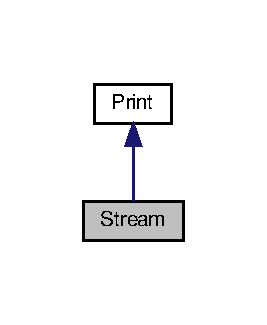
\includegraphics[width=128pt]{class_stream__inherit__graph}
\end{center}
\end{figure}


Collaboration diagram for Stream\+:\nopagebreak
\begin{figure}[H]
\begin{center}
\leavevmode
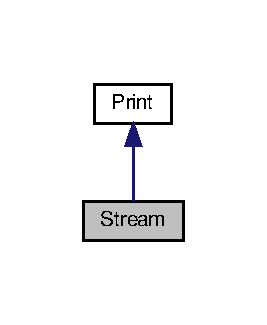
\includegraphics[width=128pt]{class_stream__coll__graph}
\end{center}
\end{figure}
\subsection*{Public Member Functions}
\begin{DoxyCompactItemize}
\item 
int \textbf{ available} ()
\item 
int \textbf{ read} ()
\item 
virtual int \textbf{ available} ()=0
\item 
virtual int \textbf{ read} ()=0
\item 
virtual int \textbf{ peek} ()=0
\item 
virtual void \textbf{ flush} ()=0
\item 
\textbf{ Stream} ()
\item 
void \textbf{ set\+Timeout} (\textbf{ system\+\_\+tick\+\_\+t} timeout)
\item 
bool \textbf{ find} (char $\ast$target)
\item 
bool \textbf{ find} (char $\ast$target, size\+\_\+t length)
\item 
bool \textbf{ find\+Until} (char $\ast$target, char $\ast$terminator)
\item 
bool \textbf{ find\+Until} (char $\ast$target, size\+\_\+t target\+Len, char $\ast$terminate, size\+\_\+t term\+Len)
\item 
long \textbf{ parse\+Int} ()
\item 
float \textbf{ parse\+Float} ()
\item 
size\+\_\+t \textbf{ read\+Bytes} (char $\ast$buffer, size\+\_\+t length)
\item 
size\+\_\+t \textbf{ read\+Bytes\+Until} (char terminator, char $\ast$buffer, size\+\_\+t length)
\item 
\textbf{ String} \textbf{ read\+String} ()
\item 
\textbf{ String} \textbf{ read\+String\+Until} (char terminator)
\end{DoxyCompactItemize}
\subsection*{Protected Member Functions}
\begin{DoxyCompactItemize}
\item 
int \textbf{ timed\+Read} ()
\item 
int \textbf{ timed\+Peek} ()
\item 
int \textbf{ peek\+Next\+Digit} ()
\item 
long \textbf{ parse\+Int} (char skip\+Char)
\item 
float \textbf{ parse\+Float} (char skip\+Char)
\end{DoxyCompactItemize}
\subsection*{Protected Attributes}
\begin{DoxyCompactItemize}
\item 
\textbf{ system\+\_\+tick\+\_\+t} \textbf{ \+\_\+timeout}
\item 
\textbf{ system\+\_\+tick\+\_\+t} \textbf{ \+\_\+start\+Millis}
\end{DoxyCompactItemize}


\subsection{Detailed Description}


Definition at line 15 of file Particle.\+h.



\subsection{Constructor \& Destructor Documentation}
\mbox{\label{class_stream_a8c3f05bd00361ec92627fa41f330a39b}} 
\index{Stream@{Stream}!Stream@{Stream}}
\index{Stream@{Stream}!Stream@{Stream}}
\subsubsection{Stream()}
{\footnotesize\ttfamily Stream\+::\+Stream (\begin{DoxyParamCaption}{ }\end{DoxyParamCaption})\hspace{0.3cm}{\ttfamily [inline]}}



Definition at line 59 of file spark\+\_\+wiring\+\_\+stream.\+h.



References \+\_\+timeout.


\begin{DoxyCode}
59 \{_timeout=1000;\}
\end{DoxyCode}


\subsection{Member Function Documentation}
\mbox{\label{class_stream_a747aa1d8db334a7b735a48dbc135478c}} 
\index{Stream@{Stream}!available@{available}}
\index{available@{available}!Stream@{Stream}}
\subsubsection{available()\hspace{0.1cm}{\footnotesize\ttfamily [1/2]}}
{\footnotesize\ttfamily int Stream\+::available (\begin{DoxyParamCaption}{ }\end{DoxyParamCaption})\hspace{0.3cm}{\ttfamily [inline]}}



Definition at line 17 of file Particle.\+h.


\begin{DoxyCode}
17 \{ \textcolor{keywordflow}{return} 0; \}
\end{DoxyCode}
\mbox{\label{class_stream_a9c98a763395005c08ce95afb2f06c7b1}} 
\index{Stream@{Stream}!available@{available}}
\index{available@{available}!Stream@{Stream}}
\subsubsection{available()\hspace{0.1cm}{\footnotesize\ttfamily [2/2]}}
{\footnotesize\ttfamily virtual int Stream\+::available (\begin{DoxyParamCaption}{ }\end{DoxyParamCaption})\hspace{0.3cm}{\ttfamily [pure virtual]}}

\mbox{\label{class_stream_a4bab30ccd324efd461dee46a2339f673}} 
\index{Stream@{Stream}!find@{find}}
\index{find@{find}!Stream@{Stream}}
\subsubsection{find()\hspace{0.1cm}{\footnotesize\ttfamily [1/2]}}
{\footnotesize\ttfamily bool Stream\+::find (\begin{DoxyParamCaption}\item[{char $\ast$}]{target }\end{DoxyParamCaption})}

\mbox{\label{class_stream_ad851401f2318cdb1de05707e021b81d9}} 
\index{Stream@{Stream}!find@{find}}
\index{find@{find}!Stream@{Stream}}
\subsubsection{find()\hspace{0.1cm}{\footnotesize\ttfamily [2/2]}}
{\footnotesize\ttfamily bool Stream\+::find (\begin{DoxyParamCaption}\item[{char $\ast$}]{target,  }\item[{size\+\_\+t}]{length }\end{DoxyParamCaption})}

\mbox{\label{class_stream_ad1f5f6600832396fb38a897baf4de35b}} 
\index{Stream@{Stream}!find\+Until@{find\+Until}}
\index{find\+Until@{find\+Until}!Stream@{Stream}}
\subsubsection{find\+Until()\hspace{0.1cm}{\footnotesize\ttfamily [1/2]}}
{\footnotesize\ttfamily bool Stream\+::find\+Until (\begin{DoxyParamCaption}\item[{char $\ast$}]{target,  }\item[{char $\ast$}]{terminator }\end{DoxyParamCaption})}

\mbox{\label{class_stream_a3a9497de614792103ab8cb4759e01a69}} 
\index{Stream@{Stream}!find\+Until@{find\+Until}}
\index{find\+Until@{find\+Until}!Stream@{Stream}}
\subsubsection{find\+Until()\hspace{0.1cm}{\footnotesize\ttfamily [2/2]}}
{\footnotesize\ttfamily bool Stream\+::find\+Until (\begin{DoxyParamCaption}\item[{char $\ast$}]{target,  }\item[{size\+\_\+t}]{target\+Len,  }\item[{char $\ast$}]{terminate,  }\item[{size\+\_\+t}]{term\+Len }\end{DoxyParamCaption})}

\mbox{\label{class_stream_aa3ef2c34f152a0b2ea8de9139b9461da}} 
\index{Stream@{Stream}!flush@{flush}}
\index{flush@{flush}!Stream@{Stream}}
\subsubsection{flush()}
{\footnotesize\ttfamily virtual void Stream\+::flush (\begin{DoxyParamCaption}{ }\end{DoxyParamCaption})\hspace{0.3cm}{\ttfamily [pure virtual]}}

\mbox{\label{class_stream_a5e5a0cc11eb586d89dcb7fa8e53a87e8}} 
\index{Stream@{Stream}!parse\+Float@{parse\+Float}}
\index{parse\+Float@{parse\+Float}!Stream@{Stream}}
\subsubsection{parse\+Float()\hspace{0.1cm}{\footnotesize\ttfamily [1/2]}}
{\footnotesize\ttfamily float Stream\+::parse\+Float (\begin{DoxyParamCaption}{ }\end{DoxyParamCaption})}

\mbox{\label{class_stream_a14a98cdbb166008f25dd044d836b1864}} 
\index{Stream@{Stream}!parse\+Float@{parse\+Float}}
\index{parse\+Float@{parse\+Float}!Stream@{Stream}}
\subsubsection{parse\+Float()\hspace{0.1cm}{\footnotesize\ttfamily [2/2]}}
{\footnotesize\ttfamily float Stream\+::parse\+Float (\begin{DoxyParamCaption}\item[{char}]{skip\+Char }\end{DoxyParamCaption})\hspace{0.3cm}{\ttfamily [protected]}}

\mbox{\label{class_stream_a497ffcbcb4d5bb889a8fde487bcc1b98}} 
\index{Stream@{Stream}!parse\+Int@{parse\+Int}}
\index{parse\+Int@{parse\+Int}!Stream@{Stream}}
\subsubsection{parse\+Int()\hspace{0.1cm}{\footnotesize\ttfamily [1/2]}}
{\footnotesize\ttfamily long Stream\+::parse\+Int (\begin{DoxyParamCaption}{ }\end{DoxyParamCaption})}

\mbox{\label{class_stream_a4578615defade6c4ce7daeb6578bb62d}} 
\index{Stream@{Stream}!parse\+Int@{parse\+Int}}
\index{parse\+Int@{parse\+Int}!Stream@{Stream}}
\subsubsection{parse\+Int()\hspace{0.1cm}{\footnotesize\ttfamily [2/2]}}
{\footnotesize\ttfamily long Stream\+::parse\+Int (\begin{DoxyParamCaption}\item[{char}]{skip\+Char }\end{DoxyParamCaption})\hspace{0.3cm}{\ttfamily [protected]}}

\mbox{\label{class_stream_a30c3c212ec6ea67277a708c5ea2501a5}} 
\index{Stream@{Stream}!peek@{peek}}
\index{peek@{peek}!Stream@{Stream}}
\subsubsection{peek()}
{\footnotesize\ttfamily virtual int Stream\+::peek (\begin{DoxyParamCaption}{ }\end{DoxyParamCaption})\hspace{0.3cm}{\ttfamily [pure virtual]}}

\mbox{\label{class_stream_ab31c533ddc422c8d8df07986e5920534}} 
\index{Stream@{Stream}!peek\+Next\+Digit@{peek\+Next\+Digit}}
\index{peek\+Next\+Digit@{peek\+Next\+Digit}!Stream@{Stream}}
\subsubsection{peek\+Next\+Digit()}
{\footnotesize\ttfamily int Stream\+::peek\+Next\+Digit (\begin{DoxyParamCaption}{ }\end{DoxyParamCaption})\hspace{0.3cm}{\ttfamily [protected]}}

\mbox{\label{class_stream_a654017caec3e3feeba5feb346d83c7bb}} 
\index{Stream@{Stream}!read@{read}}
\index{read@{read}!Stream@{Stream}}
\subsubsection{read()\hspace{0.1cm}{\footnotesize\ttfamily [1/2]}}
{\footnotesize\ttfamily int Stream\+::read (\begin{DoxyParamCaption}{ }\end{DoxyParamCaption})\hspace{0.3cm}{\ttfamily [inline]}}



Definition at line 18 of file Particle.\+h.


\begin{DoxyCode}
18 \{ \textcolor{keywordflow}{return} 0; \}
\end{DoxyCode}
\mbox{\label{class_stream_aea5dee9fcb038148515b7c9212d38dc0}} 
\index{Stream@{Stream}!read@{read}}
\index{read@{read}!Stream@{Stream}}
\subsubsection{read()\hspace{0.1cm}{\footnotesize\ttfamily [2/2]}}
{\footnotesize\ttfamily virtual int Stream\+::read (\begin{DoxyParamCaption}{ }\end{DoxyParamCaption})\hspace{0.3cm}{\ttfamily [pure virtual]}}

\mbox{\label{class_stream_a45fd1336a323ea83b16e8507055f44ea}} 
\index{Stream@{Stream}!read\+Bytes@{read\+Bytes}}
\index{read\+Bytes@{read\+Bytes}!Stream@{Stream}}
\subsubsection{read\+Bytes()}
{\footnotesize\ttfamily size\+\_\+t Stream\+::read\+Bytes (\begin{DoxyParamCaption}\item[{char $\ast$}]{buffer,  }\item[{size\+\_\+t}]{length }\end{DoxyParamCaption})}

\mbox{\label{class_stream_af84672a4fb2620466958d3118d4fea00}} 
\index{Stream@{Stream}!read\+Bytes\+Until@{read\+Bytes\+Until}}
\index{read\+Bytes\+Until@{read\+Bytes\+Until}!Stream@{Stream}}
\subsubsection{read\+Bytes\+Until()}
{\footnotesize\ttfamily size\+\_\+t Stream\+::read\+Bytes\+Until (\begin{DoxyParamCaption}\item[{char}]{terminator,  }\item[{char $\ast$}]{buffer,  }\item[{size\+\_\+t}]{length }\end{DoxyParamCaption})}

\mbox{\label{class_stream_a1c60bdda2b65d78e5a1362d51b856c5a}} 
\index{Stream@{Stream}!read\+String@{read\+String}}
\index{read\+String@{read\+String}!Stream@{Stream}}
\subsubsection{read\+String()}
{\footnotesize\ttfamily \textbf{ String} Stream\+::read\+String (\begin{DoxyParamCaption}{ }\end{DoxyParamCaption})}

\mbox{\label{class_stream_a6a409da87c552909260d8cc428c5ca70}} 
\index{Stream@{Stream}!read\+String\+Until@{read\+String\+Until}}
\index{read\+String\+Until@{read\+String\+Until}!Stream@{Stream}}
\subsubsection{read\+String\+Until()}
{\footnotesize\ttfamily \textbf{ String} Stream\+::read\+String\+Until (\begin{DoxyParamCaption}\item[{char}]{terminator }\end{DoxyParamCaption})}

\mbox{\label{class_stream_abaa50647d6dbb3baf7697a2691a06177}} 
\index{Stream@{Stream}!set\+Timeout@{set\+Timeout}}
\index{set\+Timeout@{set\+Timeout}!Stream@{Stream}}
\subsubsection{set\+Timeout()}
{\footnotesize\ttfamily void Stream\+::set\+Timeout (\begin{DoxyParamCaption}\item[{\textbf{ system\+\_\+tick\+\_\+t}}]{timeout }\end{DoxyParamCaption})}

\mbox{\label{class_stream_ae326bf60a3c5276836526710871046fe}} 
\index{Stream@{Stream}!timed\+Peek@{timed\+Peek}}
\index{timed\+Peek@{timed\+Peek}!Stream@{Stream}}
\subsubsection{timed\+Peek()}
{\footnotesize\ttfamily int Stream\+::timed\+Peek (\begin{DoxyParamCaption}{ }\end{DoxyParamCaption})\hspace{0.3cm}{\ttfamily [protected]}}

\mbox{\label{class_stream_a416a0ada5ed3c9d27f1e72c7d73f0aa1}} 
\index{Stream@{Stream}!timed\+Read@{timed\+Read}}
\index{timed\+Read@{timed\+Read}!Stream@{Stream}}
\subsubsection{timed\+Read()}
{\footnotesize\ttfamily int Stream\+::timed\+Read (\begin{DoxyParamCaption}{ }\end{DoxyParamCaption})\hspace{0.3cm}{\ttfamily [protected]}}



\subsection{Member Data Documentation}
\mbox{\label{class_stream_abbead2dae5b725a965860b65fb7f6b34}} 
\index{Stream@{Stream}!\+\_\+start\+Millis@{\+\_\+start\+Millis}}
\index{\+\_\+start\+Millis@{\+\_\+start\+Millis}!Stream@{Stream}}
\subsubsection{\+\_\+start\+Millis}
{\footnotesize\ttfamily \textbf{ system\+\_\+tick\+\_\+t} Stream\+::\+\_\+start\+Millis\hspace{0.3cm}{\ttfamily [protected]}}



Definition at line 48 of file spark\+\_\+wiring\+\_\+stream.\+h.

\mbox{\label{class_stream_ae1fc2b43124fc405406ce18b7e22d48c}} 
\index{Stream@{Stream}!\+\_\+timeout@{\+\_\+timeout}}
\index{\+\_\+timeout@{\+\_\+timeout}!Stream@{Stream}}
\subsubsection{\+\_\+timeout}
{\footnotesize\ttfamily \textbf{ system\+\_\+tick\+\_\+t} Stream\+::\+\_\+timeout\hspace{0.3cm}{\ttfamily [protected]}}



Definition at line 47 of file spark\+\_\+wiring\+\_\+stream.\+h.



Referenced by Stream().



The documentation for this class was generated from the following files\+:\begin{DoxyCompactItemize}
\item 
lib/\+Json\+Parser\+Generator\+R\+K/test/gcclib/\textbf{ Particle.\+h}\item 
lib/\+Json\+Parser\+Generator\+R\+K/test/gcclib/\textbf{ spark\+\_\+wiring\+\_\+stream.\+h}\end{DoxyCompactItemize}

\section{String Class Reference}
\label{class_string}\index{String@{String}}


Wiring \doxyref{String}{p.}{class_string}\+: A class to hold and manipulate a dynamically allocated string.  




{\ttfamily \#include $<$spark\+\_\+wiring\+\_\+string.\+h$>$}



Inheritance diagram for String\+:\nopagebreak
\begin{figure}[H]
\begin{center}
\leavevmode
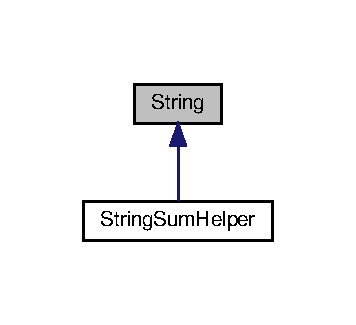
\includegraphics[width=171pt]{class_string__inherit__graph}
\end{center}
\end{figure}
\subsection*{Public Member Functions}
\begin{DoxyCompactItemize}
\item 
\textbf{ String} (const char $\ast$cstr=\char`\"{}\char`\"{})
\begin{DoxyCompactList}\small\item\em Construct a \doxyref{String}{p.}{class_string} object from a c-\/string (null-\/terminated) \end{DoxyCompactList}\item 
\textbf{ String} (const char $\ast$cstr, unsigned int \textbf{ length})
\begin{DoxyCompactList}\small\item\em Construct a \doxyref{String}{p.}{class_string} object from a pointer and length. \end{DoxyCompactList}\item 
\textbf{ String} (const \textbf{ String} \&str)
\begin{DoxyCompactList}\small\item\em Construct a \doxyref{String}{p.}{class_string} object as a copy of another string. \end{DoxyCompactList}\item 
\textbf{ String} (const \+\_\+\+\_\+\+Flash\+String\+Helper $\ast$pstr)
\item 
\textbf{ String} (const \textbf{ Printable} \&printable)
\begin{DoxyCompactList}\small\item\em Construct a \doxyref{String}{p.}{class_string} object from any \doxyref{Printable}{p.}{class_printable} object. \end{DoxyCompactList}\item 
\textbf{ String} (char c)
\begin{DoxyCompactList}\small\item\em Construct a \doxyref{String}{p.}{class_string} containing a single character. \end{DoxyCompactList}\item 
\textbf{ String} (unsigned char b, unsigned char base=10)
\begin{DoxyCompactList}\small\item\em Construct a \doxyref{String}{p.}{class_string} from a unsigned char (uint8\+\_\+t) value, expressed as a number. \end{DoxyCompactList}\item 
\textbf{ String} (int value, unsigned char base=10)
\begin{DoxyCompactList}\small\item\em Construct a \doxyref{String}{p.}{class_string} from a int (32 bit signed integer) value, expressed as a number. \end{DoxyCompactList}\item 
\textbf{ String} (unsigned int value, unsigned char base=10)
\begin{DoxyCompactList}\small\item\em Construct a \doxyref{String}{p.}{class_string} from a unsigned int (32 bit unsigned integer) value, expressed as a number. \end{DoxyCompactList}\item 
\textbf{ String} (long value, unsigned char base=10)
\begin{DoxyCompactList}\small\item\em Construct a \doxyref{String}{p.}{class_string} from a long (32 bit signed integer) value, expressed as a number. \end{DoxyCompactList}\item 
\textbf{ String} (unsigned long value, unsigned char base=10)
\begin{DoxyCompactList}\small\item\em Construct a \doxyref{String}{p.}{class_string} from a unsigned long (32 bit unsigned integer) value, expressed as a number. \end{DoxyCompactList}\item 
\textbf{ String} (float value, int decimal\+Places=6)
\begin{DoxyCompactList}\small\item\em Construct a \doxyref{String}{p.}{class_string} from a float (32 bit single precision floating point) value, expressed as a number. \end{DoxyCompactList}\item 
\textbf{ String} (double value, int decimal\+Places=6)
\begin{DoxyCompactList}\small\item\em Construct a \doxyref{String}{p.}{class_string} from a double (64 bit double precision floating point) value, expressed as a number. \end{DoxyCompactList}\item 
\textbf{ $\sim$\+String} (void)
\begin{DoxyCompactList}\small\item\em Destructor. Also deletes the underlying dynamically allocated string. \end{DoxyCompactList}\item 
unsigned char \textbf{ reserve} (unsigned int size)
\begin{DoxyCompactList}\small\item\em Reserves a buffer of size. \end{DoxyCompactList}\item 
unsigned int \textbf{ length} (void) const
\begin{DoxyCompactList}\small\item\em Returns the length of the string in bytes. \end{DoxyCompactList}\item 
\textbf{ String} \& \textbf{ operator=} (const \textbf{ String} \&rhs)
\begin{DoxyCompactList}\small\item\em Assigns this string to have a copy of \doxyref{String}{p.}{class_string} rhs. \end{DoxyCompactList}\item 
\textbf{ String} \& \textbf{ operator=} (const char $\ast$cstr)
\begin{DoxyCompactList}\small\item\em Assigns this string to have a copy of c-\/string (null-\/terminated) cstr. \end{DoxyCompactList}\item 
\textbf{ String} \& \textbf{ operator=} (const \+\_\+\+\_\+\+Flash\+String\+Helper $\ast$pstr)
\item 
\textbf{ operator const char $\ast$} () const
\begin{DoxyCompactList}\small\item\em Returns the contents this \doxyref{String}{p.}{class_string} as a c-\/string (null-\/terminated) \end{DoxyCompactList}\item 
unsigned char \textbf{ concat} (const \textbf{ String} \&str)
\begin{DoxyCompactList}\small\item\em Append (concatenate) a \doxyref{String}{p.}{class_string} object to the end of this \doxyref{String}{p.}{class_string}, modifying this string in place. \end{DoxyCompactList}\item 
unsigned char \textbf{ concat} (const char $\ast$cstr)
\begin{DoxyCompactList}\small\item\em Append (concatenate) a c-\/string (null-\/terminated) to the end of this \doxyref{String}{p.}{class_string}, modifying this string in place. \end{DoxyCompactList}\item 
unsigned char \textbf{ concat} (const \+\_\+\+\_\+\+Flash\+String\+Helper $\ast$str)
\item 
unsigned char \textbf{ concat} (char c)
\begin{DoxyCompactList}\small\item\em Append (concatenate) a single character to the end of this \doxyref{String}{p.}{class_string}, modifying this string in place. \end{DoxyCompactList}\item 
unsigned char \textbf{ concat} (unsigned char c)
\begin{DoxyCompactList}\small\item\em Append (concatenate) the byte value c to the end of this \doxyref{String}{p.}{class_string} as a decimal number 0 -\/ 255, modifying this string in place. \end{DoxyCompactList}\item 
unsigned char \textbf{ concat} (int num)
\begin{DoxyCompactList}\small\item\em Append (concatenate) the integer value num to the end of this \doxyref{String}{p.}{class_string} as a signed decimal number (base 10), modifying this string in place. \end{DoxyCompactList}\item 
unsigned char \textbf{ concat} (unsigned int num)
\begin{DoxyCompactList}\small\item\em Append (concatenate) the unsigned integer value num to the end of this \doxyref{String}{p.}{class_string} as a unsigned decimal number (base 10), modifying this string in place. \end{DoxyCompactList}\item 
unsigned char \textbf{ concat} (long num)
\begin{DoxyCompactList}\small\item\em Append (concatenate) the long integer value num to the end of this \doxyref{String}{p.}{class_string} as a signed decimal number (base 10), modifying this string in place. \end{DoxyCompactList}\item 
unsigned char \textbf{ concat} (unsigned long num)
\begin{DoxyCompactList}\small\item\em Append (concatenate) the unsigned long value num to the end of this \doxyref{String}{p.}{class_string} as a unsigned decimal number (base 10), modifying this string in place. \end{DoxyCompactList}\item 
unsigned char \textbf{ concat} (float num)
\begin{DoxyCompactList}\small\item\em Append (concatenate) the float n to the end of this \doxyref{String}{p.}{class_string} as a decimal number (base 10), modifying this string in place. \end{DoxyCompactList}\item 
unsigned char \textbf{ concat} (double num)
\begin{DoxyCompactList}\small\item\em Append (concatenate) the double precision float n to the end of this \doxyref{String}{p.}{class_string} as a decimal number (base 10), modifying this string in place. \end{DoxyCompactList}\item 
\textbf{ String} \& \textbf{ operator+=} (const \textbf{ String} \&rhs)
\begin{DoxyCompactList}\small\item\em Appends (concatenate) a \doxyref{String}{p.}{class_string} object to the end of this \doxyref{String}{p.}{class_string}, modifying this string in place. \end{DoxyCompactList}\item 
\textbf{ String} \& \textbf{ operator+=} (const char $\ast$cstr)
\begin{DoxyCompactList}\small\item\em Appends (concatenate) a c-\/string (null-\/terminated) to the end of this \doxyref{String}{p.}{class_string}, modifying this string in place. \end{DoxyCompactList}\item 
\textbf{ String} \& \textbf{ operator+=} (char c)
\begin{DoxyCompactList}\small\item\em Appends (concatenate) a single character to the end of this \doxyref{String}{p.}{class_string}, modifying this string in place. \end{DoxyCompactList}\item 
\textbf{ String} \& \textbf{ operator+=} (unsigned char num)
\begin{DoxyCompactList}\small\item\em Append (concatenate) the byte value num to the end of this \doxyref{String}{p.}{class_string} as a decimal number 0 -\/ 255, modifying this string in place. \end{DoxyCompactList}\item 
\textbf{ String} \& \textbf{ operator+=} (int num)
\begin{DoxyCompactList}\small\item\em Append (concatenate) the integer value num to the end of this \doxyref{String}{p.}{class_string} as a signed decimal number (base 10), modifying this string in place. \end{DoxyCompactList}\item 
\textbf{ String} \& \textbf{ operator+=} (unsigned int num)
\begin{DoxyCompactList}\small\item\em Append (concatenate) the unsigned integer value num to the end of this \doxyref{String}{p.}{class_string} as a unsigned decimal number (base 10), modifying this string in place. \end{DoxyCompactList}\item 
\textbf{ String} \& \textbf{ operator+=} (long num)
\begin{DoxyCompactList}\small\item\em Append (concatenate) the long integer value num to the end of this \doxyref{String}{p.}{class_string} as a signed decimal number (base 10), modifying this string in place. \end{DoxyCompactList}\item 
\textbf{ String} \& \textbf{ operator+=} (unsigned long num)
\begin{DoxyCompactList}\small\item\em Append (concatenate) the unsigned long value num to the end of this \doxyref{String}{p.}{class_string} as a unsigned decimal number (base 10), modifying this string in place. \end{DoxyCompactList}\item 
\textbf{ operator String\+If\+Helper\+Type} () const
\item 
int \textbf{ compare\+To} (const \textbf{ String} \&s) const
\begin{DoxyCompactList}\small\item\em Compares this string to another string using strcmp (case-\/sensitive) \end{DoxyCompactList}\item 
unsigned char \textbf{ equals} (const \textbf{ String} \&s) const
\begin{DoxyCompactList}\small\item\em Returns true if this string is equal to another string (case-\/sensitive) \end{DoxyCompactList}\item 
unsigned char \textbf{ equals} (const char $\ast$cstr) const
\begin{DoxyCompactList}\small\item\em Returns true if this string equal to another string (case-\/sensitive) \end{DoxyCompactList}\item 
unsigned char \textbf{ operator==} (const \textbf{ String} \&rhs) const
\begin{DoxyCompactList}\small\item\em Returns true if this string is equal to another string (case-\/sensitive) \end{DoxyCompactList}\item 
unsigned char \textbf{ operator==} (const char $\ast$cstr) const
\begin{DoxyCompactList}\small\item\em Returns true if this string equal to another string (case-\/sensitive) \end{DoxyCompactList}\item 
unsigned char \textbf{ operator!=} (const \textbf{ String} \&rhs) const
\begin{DoxyCompactList}\small\item\em Returns true if this string is greater than to another string (case-\/sensitive) \end{DoxyCompactList}\item 
unsigned char \textbf{ operator!=} (const char $\ast$cstr) const
\begin{DoxyCompactList}\small\item\em Returns true if this string not equal to another string (case-\/sensitive) \end{DoxyCompactList}\item 
unsigned char \textbf{ operator$<$} (const \textbf{ String} \&rhs) const
\begin{DoxyCompactList}\small\item\em Returns true if this string is less than to another string (case-\/sensitive) \end{DoxyCompactList}\item 
unsigned char \textbf{ operator$>$} (const \textbf{ String} \&rhs) const
\begin{DoxyCompactList}\small\item\em Returns true if this string is greater than to another string (case-\/sensitive) \end{DoxyCompactList}\item 
unsigned char \textbf{ operator$<$=} (const \textbf{ String} \&rhs) const
\begin{DoxyCompactList}\small\item\em Returns true if this string is less than or equal to another string (case-\/sensitive) \end{DoxyCompactList}\item 
unsigned char \textbf{ operator$>$=} (const \textbf{ String} \&rhs) const
\begin{DoxyCompactList}\small\item\em Returns true if this string is greater than or equal to another string (case-\/sensitive) \end{DoxyCompactList}\item 
unsigned char \textbf{ equals\+Ignore\+Case} (const \textbf{ String} \&s) const
\begin{DoxyCompactList}\small\item\em Returns true if this string equals another string (case-\/insensitive) \end{DoxyCompactList}\item 
unsigned char \textbf{ starts\+With} (const \textbf{ String} \&prefix) const
\begin{DoxyCompactList}\small\item\em Returns true if this string starts with prefix (case-\/sensitive) \end{DoxyCompactList}\item 
unsigned char \textbf{ starts\+With} (const \textbf{ String} \&prefix, unsigned int offset) const
\begin{DoxyCompactList}\small\item\em Returns true if this string contains prefix at specified offset (case-\/sensitive) \end{DoxyCompactList}\item 
unsigned char \textbf{ ends\+With} (const \textbf{ String} \&suffix) const
\begin{DoxyCompactList}\small\item\em Returns true if this string ends with suffix (case-\/sensitive) \end{DoxyCompactList}\item 
char \textbf{ char\+At} (unsigned int index) const
\begin{DoxyCompactList}\small\item\em Gets the character at offset index. \end{DoxyCompactList}\item 
void \textbf{ set\+Char\+At} (unsigned int index, char c)
\begin{DoxyCompactList}\small\item\em Set the character at offset index. \end{DoxyCompactList}\item 
char \textbf{ operator[$\,$]} (unsigned int index) const
\begin{DoxyCompactList}\small\item\em Gets the character at offset index. \end{DoxyCompactList}\item 
char \& \textbf{ operator[$\,$]} (unsigned int index)
\begin{DoxyCompactList}\small\item\em Set the character at offset index. \end{DoxyCompactList}\item 
void \textbf{ get\+Bytes} (unsigned char $\ast$buf, unsigned int bufsize, unsigned int index=0) const
\begin{DoxyCompactList}\small\item\em Copy the data out of this \doxyref{String}{p.}{class_string} into another buffer. \end{DoxyCompactList}\item 
void \textbf{ to\+Char\+Array} (char $\ast$buf, unsigned int bufsize, unsigned int index=0) const
\begin{DoxyCompactList}\small\item\em Copy the data out of this \doxyref{String}{p.}{class_string} into another buffer. \end{DoxyCompactList}\item 
const char $\ast$ \textbf{ c\+\_\+str} () const
\begin{DoxyCompactList}\small\item\em Returns a c-\/string (null-\/terminated) \end{DoxyCompactList}\item 
int \textbf{ index\+Of} (char ch) const
\begin{DoxyCompactList}\small\item\em Search this string for a given character. \end{DoxyCompactList}\item 
int \textbf{ index\+Of} (char ch, unsigned int from\+Index) const
\begin{DoxyCompactList}\small\item\em Search this string for a given character starting at an offset. \end{DoxyCompactList}\item 
int \textbf{ index\+Of} (const \textbf{ String} \&str) const
\begin{DoxyCompactList}\small\item\em Search this string for a given \doxyref{String}{p.}{class_string}. \end{DoxyCompactList}\item 
int \textbf{ index\+Of} (const \textbf{ String} \&str, unsigned int from\+Index) const
\begin{DoxyCompactList}\small\item\em Search this string for a given \doxyref{String}{p.}{class_string} starting at an offset. \end{DoxyCompactList}\item 
int \textbf{ last\+Index\+Of} (char ch) const
\begin{DoxyCompactList}\small\item\em Search this string for a given character, starting at the end. \end{DoxyCompactList}\item 
int \textbf{ last\+Index\+Of} (char ch, unsigned int from\+Index) const
\begin{DoxyCompactList}\small\item\em Search this string for a given character, starting at the from\+Index and going toward the beginning. \end{DoxyCompactList}\item 
int \textbf{ last\+Index\+Of} (const \textbf{ String} \&str) const
\begin{DoxyCompactList}\small\item\em Search this string for a last occurrence of str. \end{DoxyCompactList}\item 
int \textbf{ last\+Index\+Of} (const \textbf{ String} \&str, unsigned int from\+Index) const
\begin{DoxyCompactList}\small\item\em Search this string for a last occurrence of str starting at from\+Index. \end{DoxyCompactList}\item 
\textbf{ String} \textbf{ substring} (unsigned int begin\+Index) const
\begin{DoxyCompactList}\small\item\em Returns a \doxyref{String}{p.}{class_string} object with a copy of the characters starting at begin\+Index through the end of the string. \end{DoxyCompactList}\item 
\textbf{ String} \textbf{ substring} (unsigned int begin\+Index, unsigned int end\+Index) const
\begin{DoxyCompactList}\small\item\em Returns a \doxyref{String}{p.}{class_string} object with a copy of the characters in the specified range. \end{DoxyCompactList}\item 
\textbf{ String} \& \textbf{ replace} (char find, char replace)
\begin{DoxyCompactList}\small\item\em Replaces every occurrence of a character in the string with another character, modifying it in place. \end{DoxyCompactList}\item 
\textbf{ String} \& \textbf{ replace} (const \textbf{ String} \&find, const \textbf{ String} \&replace)
\begin{DoxyCompactList}\small\item\em Replaces every occurrence of a \doxyref{String}{p.}{class_string} with another \doxyref{String}{p.}{class_string}, modifying it in place. \end{DoxyCompactList}\item 
\textbf{ String} \& \textbf{ remove} (unsigned int index)
\begin{DoxyCompactList}\small\item\em Removes characters from the \doxyref{String}{p.}{class_string}, modifying it in place. \end{DoxyCompactList}\item 
\textbf{ String} \& \textbf{ remove} (unsigned int index, unsigned int count)
\begin{DoxyCompactList}\small\item\em Removes characters from the \doxyref{String}{p.}{class_string}, modifying it in place. \end{DoxyCompactList}\item 
\textbf{ String} \& \textbf{ to\+Lower\+Case} (void)
\begin{DoxyCompactList}\small\item\em Converts this \doxyref{String}{p.}{class_string} to lower case, modifying it in place. \end{DoxyCompactList}\item 
\textbf{ String} \& \textbf{ to\+Upper\+Case} (void)
\begin{DoxyCompactList}\small\item\em Converts this \doxyref{String}{p.}{class_string} to upper case, modifying it in place. \end{DoxyCompactList}\item 
\textbf{ String} \& \textbf{ trim} (void)
\begin{DoxyCompactList}\small\item\em Removes leading an trailing white spaces from this string, modifying it in place. \end{DoxyCompactList}\item 
long \textbf{ to\+Int} (void) const
\begin{DoxyCompactList}\small\item\em Converts this string to a signed integer (32-\/bit) \end{DoxyCompactList}\item 
float \textbf{ to\+Float} (void) const
\begin{DoxyCompactList}\small\item\em Converts this string to a float (single precision floating point value) \end{DoxyCompactList}\end{DoxyCompactItemize}
\subsection*{Static Public Member Functions}
\begin{DoxyCompactItemize}
\item 
static \textbf{ String} \textbf{ format} (const char $\ast$format,...)
\begin{DoxyCompactList}\small\item\em Uses sprintf-\/style formatting to build a \doxyref{String}{p.}{class_string} object [static]. \end{DoxyCompactList}\end{DoxyCompactItemize}
\subsection*{Protected Member Functions}
\begin{DoxyCompactItemize}
\item 
void \textbf{ init} (void)
\item 
void \textbf{ invalidate} (void)
\item 
unsigned char \textbf{ change\+Buffer} (unsigned int max\+Str\+Len)
\item 
unsigned char \textbf{ concat} (const char $\ast$cstr, unsigned int \textbf{ length})
\item 
\textbf{ String} \& \textbf{ copy} (const char $\ast$cstr, unsigned int \textbf{ length})
\item 
\textbf{ String} \& \textbf{ copy} (const \+\_\+\+\_\+\+Flash\+String\+Helper $\ast$pstr, unsigned int \textbf{ length})
\end{DoxyCompactItemize}
\subsection*{Protected Attributes}
\begin{DoxyCompactItemize}
\item 
char $\ast$ \textbf{ buffer}
\begin{DoxyCompactList}\small\item\em The buffer containing the data. It is always null-\/terminated. \end{DoxyCompactList}\item 
unsigned int \textbf{ capacity}
\begin{DoxyCompactList}\small\item\em The capacity of the buffer. The longest string is one byte less than this. \end{DoxyCompactList}\item 
unsigned int \textbf{ len}
\begin{DoxyCompactList}\small\item\em The \doxyref{String}{p.}{class_string} length (not counting the null terminator). \end{DoxyCompactList}\item 
unsigned char \textbf{ flags}
\begin{DoxyCompactList}\small\item\em Unused, for future features. \end{DoxyCompactList}\end{DoxyCompactItemize}
\subsection*{Private Types}
\begin{DoxyCompactItemize}
\item 
typedef void(String\+::$\ast$ \textbf{ String\+If\+Helper\+Type}) () const
\end{DoxyCompactItemize}
\subsection*{Private Member Functions}
\begin{DoxyCompactItemize}
\item 
void \textbf{ String\+If\+Helper} () const
\end{DoxyCompactItemize}
\subsection*{Friends}
\begin{DoxyCompactItemize}
\item 
class \textbf{ String\+Printable\+Helper}
\item 
\textbf{ String\+Sum\+Helper} \& \textbf{ operator+} (const \textbf{ String\+Sum\+Helper} \&lhs, const \textbf{ String} \&rhs)
\begin{DoxyCompactList}\small\item\em Append (concatenate) a \doxyref{String}{p.}{class_string} to the end of lhs. \end{DoxyCompactList}\item 
\textbf{ String\+Sum\+Helper} \& \textbf{ operator+} (const \textbf{ String\+Sum\+Helper} \&lhs, const char $\ast$cstr)
\begin{DoxyCompactList}\small\item\em Append (concatenate) a c-\/string (null-\/terminated) to the end of lhs. \end{DoxyCompactList}\item 
\textbf{ String\+Sum\+Helper} \& \textbf{ operator+} (const \textbf{ String\+Sum\+Helper} \&lhs, char c)
\begin{DoxyCompactList}\small\item\em Append (concatenate) the character c the end of lhs a. \end{DoxyCompactList}\item 
\textbf{ String\+Sum\+Helper} \& \textbf{ operator+} (const \textbf{ String\+Sum\+Helper} \&lhs, unsigned char num)
\begin{DoxyCompactList}\small\item\em Append (concatenate) the unsigned char num to the end of lhs as a decimal number (base 10) \end{DoxyCompactList}\item 
\textbf{ String\+Sum\+Helper} \& \textbf{ operator+} (const \textbf{ String\+Sum\+Helper} \&lhs, int num)
\begin{DoxyCompactList}\small\item\em Append (concatenate) the signed int num to the end of lhs as a decimal number (base 10) \end{DoxyCompactList}\item 
\textbf{ String\+Sum\+Helper} \& \textbf{ operator+} (const \textbf{ String\+Sum\+Helper} \&lhs, unsigned int num)
\begin{DoxyCompactList}\small\item\em Append (concatenate) the unsigned int num to the end of lhs as a decimal number (base 10) \end{DoxyCompactList}\item 
\textbf{ String\+Sum\+Helper} \& \textbf{ operator+} (const \textbf{ String\+Sum\+Helper} \&lhs, long num)
\begin{DoxyCompactList}\small\item\em Append (concatenate) the long integer num to the end of lhs as a decimal number (base 10) \end{DoxyCompactList}\item 
\textbf{ String\+Sum\+Helper} \& \textbf{ operator+} (const \textbf{ String\+Sum\+Helper} \&lhs, unsigned long num)
\begin{DoxyCompactList}\small\item\em Append (concatenate) the unsigned long integer to the end of lhs as a decimal number (base 10) \end{DoxyCompactList}\item 
\textbf{ String\+Sum\+Helper} \& \textbf{ operator+} (const \textbf{ String\+Sum\+Helper} \&lhs, float num)
\begin{DoxyCompactList}\small\item\em Append (concatenate) the float num to the end of lhs as a decimal number (base 10) \end{DoxyCompactList}\item 
\textbf{ String\+Sum\+Helper} \& \textbf{ operator+} (const \textbf{ String\+Sum\+Helper} \&lhs, double num)
\begin{DoxyCompactList}\small\item\em Append (concatenate) the double precision float num to the end of lhs as a decimal number (base 10) \end{DoxyCompactList}\end{DoxyCompactItemize}


\subsection{Detailed Description}
Wiring \doxyref{String}{p.}{class_string}\+: A class to hold and manipulate a dynamically allocated string. 

Definition at line 54 of file spark\+\_\+wiring\+\_\+string.\+h.



\subsection{Member Typedef Documentation}
\mbox{\label{class_string_a2f31c4cd9dab650141b50a8350a1ffd4}} 
\index{String@{String}!String\+If\+Helper\+Type@{String\+If\+Helper\+Type}}
\index{String\+If\+Helper\+Type@{String\+If\+Helper\+Type}!String@{String}}
\subsubsection{String\+If\+Helper\+Type}
{\footnotesize\ttfamily typedef void(String\+::$\ast$ String\+::\+String\+If\+Helper\+Type) () const\hspace{0.3cm}{\ttfamily [private]}}



Definition at line 59 of file spark\+\_\+wiring\+\_\+string.\+h.



\subsection{Constructor \& Destructor Documentation}
\mbox{\label{class_string_a9c6238ddd5e2dca198ead5227fc7b858}} 
\index{String@{String}!String@{String}}
\index{String@{String}!String@{String}}
\subsubsection{String()\hspace{0.1cm}{\footnotesize\ttfamily [1/13]}}
{\footnotesize\ttfamily String\+::\+String (\begin{DoxyParamCaption}\item[{const char $\ast$}]{cstr = {\ttfamily \char`\"{}\char`\"{}} }\end{DoxyParamCaption})}



Construct a \doxyref{String}{p.}{class_string} object from a c-\/string (null-\/terminated) 


\begin{DoxyParams}{Parameters}
{\em cstr} & The string to copy, optional. If not specified, starts with an empty string \\
\hline
\end{DoxyParams}


Definition at line 69 of file spark\+\_\+wiring\+\_\+string.\+cpp.



References copy(), and init().



Referenced by String\+Sum\+Helper\+::\+String\+Sum\+Helper().


\begin{DoxyCode}
70 \{
71     init();
72     \textcolor{keywordflow}{if} (cstr) copy(cstr, strlen(cstr));
73 \}
\end{DoxyCode}
\mbox{\label{class_string_a20cfefac6f5b37f40dcb35826b563a5a}} 
\index{String@{String}!String@{String}}
\index{String@{String}!String@{String}}
\subsubsection{String()\hspace{0.1cm}{\footnotesize\ttfamily [2/13]}}
{\footnotesize\ttfamily String\+::\+String (\begin{DoxyParamCaption}\item[{const char $\ast$}]{cstr,  }\item[{unsigned int}]{length }\end{DoxyParamCaption})}



Construct a \doxyref{String}{p.}{class_string} object from a pointer and length. 


\begin{DoxyParams}{Parameters}
{\em cstr} & Pointer to a bytes, typically A\+S\+C\+II or U\+T\+F-\/8. Does not need to be null-\/terminated.\\
\hline
{\em length} & Length in bytes of the string. \\
\hline
\end{DoxyParams}
\mbox{\label{class_string_a5774bcd4a4c232a8aec5a3ec6d01a157}} 
\index{String@{String}!String@{String}}
\index{String@{String}!String@{String}}
\subsubsection{String()\hspace{0.1cm}{\footnotesize\ttfamily [3/13]}}
{\footnotesize\ttfamily String\+::\+String (\begin{DoxyParamCaption}\item[{const \textbf{ String} \&}]{str }\end{DoxyParamCaption})}



Construct a \doxyref{String}{p.}{class_string} object as a copy of another string. 


\begin{DoxyParams}{Parameters}
{\em str} & The string to copy. Changes made to str in the future won\textquotesingle{}t be reflected in this copy. \\
\hline
\end{DoxyParams}


Definition at line 75 of file spark\+\_\+wiring\+\_\+string.\+cpp.



References init(), and operator=().



Referenced by String\+Sum\+Helper\+::\+String\+Sum\+Helper().


\begin{DoxyCode}
76 \{
77     init();
78     *\textcolor{keyword}{this} = value;
79 \}
\end{DoxyCode}
\mbox{\label{class_string_a8c89c89e3cb69407bf55443c3d9dce0c}} 
\index{String@{String}!String@{String}}
\index{String@{String}!String@{String}}
\subsubsection{String()\hspace{0.1cm}{\footnotesize\ttfamily [4/13]}}
{\footnotesize\ttfamily String\+::\+String (\begin{DoxyParamCaption}\item[{const \+\_\+\+\_\+\+Flash\+String\+Helper $\ast$}]{pstr }\end{DoxyParamCaption})}

\mbox{\label{class_string_ad61d0ac2a1ff6e81fc7da8097be3c4dd}} 
\index{String@{String}!String@{String}}
\index{String@{String}!String@{String}}
\subsubsection{String()\hspace{0.1cm}{\footnotesize\ttfamily [5/13]}}
{\footnotesize\ttfamily String\+::\+String (\begin{DoxyParamCaption}\item[{const \textbf{ Printable} \&}]{printable }\end{DoxyParamCaption})}



Construct a \doxyref{String}{p.}{class_string} object from any \doxyref{Printable}{p.}{class_printable} object. 


\begin{DoxyParams}{Parameters}
{\em printable} & The \doxyref{Printable}{p.}{class_printable} object. The to\+Print() method will be called on it to print to this \doxyref{String}{p.}{class_string} the textual representation of the object.\\
\hline
\end{DoxyParams}
For example, I\+P\+Address is printable, so you can pass an I\+P\+Address to this constructor and this string will contain a textual representation of the I\+P\+Address (dotted quad). 

Definition at line 780 of file spark\+\_\+wiring\+\_\+string.\+cpp.



References init(), Printable\+::print\+To(), and String\+Printable\+Helper\+::\+String\+Printable\+Helper().


\begin{DoxyCode}
781 \{
782     init();
783     StringPrintableHelper help(*\textcolor{keyword}{this});
784     printable.printTo(help);
785 \}
\end{DoxyCode}
\mbox{\label{class_string_a1fdfe981d2c5e0075c1669dd94553082}} 
\index{String@{String}!String@{String}}
\index{String@{String}!String@{String}}
\subsubsection{String()\hspace{0.1cm}{\footnotesize\ttfamily [6/13]}}
{\footnotesize\ttfamily String\+::\+String (\begin{DoxyParamCaption}\item[{char}]{c }\end{DoxyParamCaption})\hspace{0.3cm}{\ttfamily [explicit]}}



Construct a \doxyref{String}{p.}{class_string} containing a single character. 


\begin{DoxyParams}{Parameters}
{\em c} & The character to set the \doxyref{String}{p.}{class_string} to \\
\hline
\end{DoxyParams}


Definition at line 94 of file spark\+\_\+wiring\+\_\+string.\+cpp.



References init(), and operator=().



Referenced by String\+Sum\+Helper\+::\+String\+Sum\+Helper().


\begin{DoxyCode}
95 \{
96     init();
97     \textcolor{keywordtype}{char} buf[2];
98     buf[0] = c;
99     buf[1] = 0;
100     *\textcolor{keyword}{this} = buf;
101 \}
\end{DoxyCode}
\mbox{\label{class_string_adb05525482f5991815322239e5504539}} 
\index{String@{String}!String@{String}}
\index{String@{String}!String@{String}}
\subsubsection{String()\hspace{0.1cm}{\footnotesize\ttfamily [7/13]}}
{\footnotesize\ttfamily String\+::\+String (\begin{DoxyParamCaption}\item[{unsigned char}]{b,  }\item[{unsigned char}]{base = {\ttfamily 10} }\end{DoxyParamCaption})\hspace{0.3cm}{\ttfamily [explicit]}}



Construct a \doxyref{String}{p.}{class_string} from a unsigned char (uint8\+\_\+t) value, expressed as a number. 


\begin{DoxyParams}{Parameters}
{\em b} & The value.\\
\hline
{\em base} & The number base, default is 10 (decimal). Other values include 8 (octal) and 16 (hexadecimal). \\
\hline
\end{DoxyParams}


Definition at line 103 of file spark\+\_\+wiring\+\_\+string.\+cpp.



References init(), operator=(), and utoa().



Referenced by String\+Sum\+Helper\+::\+String\+Sum\+Helper().


\begin{DoxyCode}
104 \{
105     init();
106     \textcolor{keywordtype}{char} buf[9];
107     utoa(value, buf, base);
108     *\textcolor{keyword}{this} = buf;
109 \}
\end{DoxyCode}
\mbox{\label{class_string_a5528e1c6d322a9ee21f155c291ea67d1}} 
\index{String@{String}!String@{String}}
\index{String@{String}!String@{String}}
\subsubsection{String()\hspace{0.1cm}{\footnotesize\ttfamily [8/13]}}
{\footnotesize\ttfamily String\+::\+String (\begin{DoxyParamCaption}\item[{int}]{value,  }\item[{unsigned char}]{base = {\ttfamily 10} }\end{DoxyParamCaption})\hspace{0.3cm}{\ttfamily [explicit]}}



Construct a \doxyref{String}{p.}{class_string} from a int (32 bit signed integer) value, expressed as a number. 


\begin{DoxyParams}{Parameters}
{\em value} & The value.\\
\hline
{\em base} & The number base, default is 10 (decimal). Other values include 8 (octal) and 16 (hexadecimal). \\
\hline
\end{DoxyParams}


Definition at line 111 of file spark\+\_\+wiring\+\_\+string.\+cpp.



References init(), itoa(), and operator=().



Referenced by String\+Sum\+Helper\+::\+String\+Sum\+Helper().


\begin{DoxyCode}
112 \{
113     init();
114     \textcolor{keywordtype}{char} buf[34];
115     itoa(value, buf, base);
116     *\textcolor{keyword}{this} = buf;
117 \}
\end{DoxyCode}
\mbox{\label{class_string_a53134e2b38eb0d114f886e807a3753ae}} 
\index{String@{String}!String@{String}}
\index{String@{String}!String@{String}}
\subsubsection{String()\hspace{0.1cm}{\footnotesize\ttfamily [9/13]}}
{\footnotesize\ttfamily String\+::\+String (\begin{DoxyParamCaption}\item[{unsigned int}]{value,  }\item[{unsigned char}]{base = {\ttfamily 10} }\end{DoxyParamCaption})\hspace{0.3cm}{\ttfamily [explicit]}}



Construct a \doxyref{String}{p.}{class_string} from a unsigned int (32 bit unsigned integer) value, expressed as a number. 


\begin{DoxyParams}{Parameters}
{\em value} & The value.\\
\hline
{\em base} & The number base, default is 10 (decimal). Other values include 8 (octal) and 16 (hexadecimal). \\
\hline
\end{DoxyParams}


Definition at line 119 of file spark\+\_\+wiring\+\_\+string.\+cpp.



References init(), operator=(), and utoa().



Referenced by max\+Current\+C1\+\_\+test(), max\+Current\+C2\+\_\+test(), and String\+Sum\+Helper\+::\+String\+Sum\+Helper().


\begin{DoxyCode}
120 \{
121     init();
122     \textcolor{keywordtype}{char} buf[33];
123     utoa(value, buf, base);
124     *\textcolor{keyword}{this} = buf;
125 \}
\end{DoxyCode}
\mbox{\label{class_string_a868687056546919b7109c0801d75ec83}} 
\index{String@{String}!String@{String}}
\index{String@{String}!String@{String}}
\subsubsection{String()\hspace{0.1cm}{\footnotesize\ttfamily [10/13]}}
{\footnotesize\ttfamily String\+::\+String (\begin{DoxyParamCaption}\item[{long}]{value,  }\item[{unsigned char}]{base = {\ttfamily 10} }\end{DoxyParamCaption})\hspace{0.3cm}{\ttfamily [explicit]}}



Construct a \doxyref{String}{p.}{class_string} from a long (32 bit signed integer) value, expressed as a number. 


\begin{DoxyParams}{Parameters}
{\em value} & The value.\\
\hline
{\em base} & The number base, default is 10 (decimal). Other values include 8 (octal) and 16 (hexadecimal). \\
\hline
\end{DoxyParams}


Definition at line 127 of file spark\+\_\+wiring\+\_\+string.\+cpp.



References init(), ltoa(), and operator=().



Referenced by String\+Sum\+Helper\+::\+String\+Sum\+Helper().


\begin{DoxyCode}
128 \{
129     init();
130     \textcolor{keywordtype}{char} buf[34];
131     ltoa(value, buf, base);
132     *\textcolor{keyword}{this} = buf;
133 \}
\end{DoxyCode}
\mbox{\label{class_string_abdad234c756b44cce55c75db24fddecf}} 
\index{String@{String}!String@{String}}
\index{String@{String}!String@{String}}
\subsubsection{String()\hspace{0.1cm}{\footnotesize\ttfamily [11/13]}}
{\footnotesize\ttfamily String\+::\+String (\begin{DoxyParamCaption}\item[{unsigned long}]{value,  }\item[{unsigned char}]{base = {\ttfamily 10} }\end{DoxyParamCaption})\hspace{0.3cm}{\ttfamily [explicit]}}



Construct a \doxyref{String}{p.}{class_string} from a unsigned long (32 bit unsigned integer) value, expressed as a number. 


\begin{DoxyParams}{Parameters}
{\em value} & The value.\\
\hline
{\em base} & The number base, default is 10 (decimal). Other values include 8 (octal) and 16 (hexadecimal). \\
\hline
\end{DoxyParams}


Definition at line 135 of file spark\+\_\+wiring\+\_\+string.\+cpp.



References init(), operator=(), and ultoa().



Referenced by String\+Sum\+Helper\+::\+String\+Sum\+Helper().


\begin{DoxyCode}
136 \{
137     init();
138     \textcolor{keywordtype}{char} buf[33];
139     ultoa(value, buf, base);
140     *\textcolor{keyword}{this} = buf;
141 \}
\end{DoxyCode}
\mbox{\label{class_string_adef4f199739444a78803c4043ad3e228}} 
\index{String@{String}!String@{String}}
\index{String@{String}!String@{String}}
\subsubsection{String()\hspace{0.1cm}{\footnotesize\ttfamily [12/13]}}
{\footnotesize\ttfamily String\+::\+String (\begin{DoxyParamCaption}\item[{float}]{value,  }\item[{int}]{decimal\+Places = {\ttfamily 6} }\end{DoxyParamCaption})\hspace{0.3cm}{\ttfamily [explicit]}}



Construct a \doxyref{String}{p.}{class_string} from a float (32 bit single precision floating point) value, expressed as a number. 


\begin{DoxyParams}{Parameters}
{\em value} & The value.\\
\hline
{\em decimal\+Places} & The number of decimal places to show. Default = 6. \\
\hline
\end{DoxyParams}


Definition at line 143 of file spark\+\_\+wiring\+\_\+string.\+cpp.



References dtoa(), init(), and operator=().


\begin{DoxyCode}
144 \{
145     init();
146     \textcolor{keywordtype}{char} buf[33];
147     dtoa(value, decimalPlaces, buf);
148         *\textcolor{keyword}{this} = buf;
149 \}
\end{DoxyCode}
\mbox{\label{class_string_a46e13b4608fbe763b4fc5bf22362078e}} 
\index{String@{String}!String@{String}}
\index{String@{String}!String@{String}}
\subsubsection{String()\hspace{0.1cm}{\footnotesize\ttfamily [13/13]}}
{\footnotesize\ttfamily String\+::\+String (\begin{DoxyParamCaption}\item[{double}]{value,  }\item[{int}]{decimal\+Places = {\ttfamily 6} }\end{DoxyParamCaption})\hspace{0.3cm}{\ttfamily [explicit]}}



Construct a \doxyref{String}{p.}{class_string} from a double (64 bit double precision floating point) value, expressed as a number. 


\begin{DoxyParams}{Parameters}
{\em value} & The value.\\
\hline
{\em decimal\+Places} & The number of decimal places to show. Default = 6. \\
\hline
\end{DoxyParams}


Definition at line 151 of file spark\+\_\+wiring\+\_\+string.\+cpp.



References dtoa(), init(), and operator=().


\begin{DoxyCode}
152 \{
153     init();
154     \textcolor{keywordtype}{char} buf[33];
155     dtoa(value, decimalPlaces, buf);
156         *\textcolor{keyword}{this} = buf;
157 \}
\end{DoxyCode}
\mbox{\label{class_string_ab4027f1abc8f8c0134f6098126de71e5}} 
\index{String@{String}!````~String@{$\sim$\+String}}
\index{````~String@{$\sim$\+String}!String@{String}}
\subsubsection{$\sim$\+String()}
{\footnotesize\ttfamily String\+::$\sim$\+String (\begin{DoxyParamCaption}\item[{void}]{ }\end{DoxyParamCaption})}



Destructor. Also deletes the underlying dynamically allocated string. 



Definition at line 158 of file spark\+\_\+wiring\+\_\+string.\+cpp.



References buffer.


\begin{DoxyCode}
159 \{
160     free(buffer);
161 \}
\end{DoxyCode}


\subsection{Member Function Documentation}
\mbox{\label{class_string_a0274f3e61533d15086816fb7f47ccb54}} 
\index{String@{String}!c\+\_\+str@{c\+\_\+str}}
\index{c\+\_\+str@{c\+\_\+str}!String@{String}}
\subsubsection{c\+\_\+str()}
{\footnotesize\ttfamily const char$\ast$ String\+::c\+\_\+str (\begin{DoxyParamCaption}{ }\end{DoxyParamCaption}) const\hspace{0.3cm}{\ttfamily [inline]}}



Returns a c-\/string (null-\/terminated) 

This allows the \doxyref{String}{p.}{class_string} object to be passed to anything that requires a c-\/string. See also operator const char $\ast$.

One place where you need to explicitly use \doxyref{c\+\_\+str()}{p.}{class_string_a0274f3e61533d15086816fb7f47ccb54} or cast is when passing a \doxyref{String}{p.}{class_string} as a variable argument to sprintf\+:


\begin{DoxyCode}
String str;
snprintf(buf, \textcolor{keyword}{sizeof}(buf), \textcolor{stringliteral}{"string=%s"}, str.c_str());
\end{DoxyCode}


If you leave off the \doxyref{c\+\_\+str()}{p.}{class_string_a0274f3e61533d15086816fb7f47ccb54} the value won\textquotesingle{}t be printed as string. This also applies to things that use sprintf internally, like Log\+:


\begin{DoxyCode}
Log.info(\textcolor{stringliteral}{"string=%s"}, str.c_str());
\end{DoxyCode}


This method returns a pointer to the internal buffer. If the underlying string is reallocated because the string is appended to, this pointer will be invalid. 

Definition at line 819 of file spark\+\_\+wiring\+\_\+string.\+h.



References buffer.



Referenced by Json\+Writer\+::insert\+Value(), main(), operator const char $\ast$(), and operator$<$$<$().


\begin{DoxyCode}
819 \{ \textcolor{keywordflow}{return} buffer; \}
\end{DoxyCode}
\mbox{\label{class_string_aea30ddc42b0dd5434d23606c39580e5d}} 
\index{String@{String}!change\+Buffer@{change\+Buffer}}
\index{change\+Buffer@{change\+Buffer}!String@{String}}
\subsubsection{change\+Buffer()}
{\footnotesize\ttfamily unsigned char String\+::change\+Buffer (\begin{DoxyParamCaption}\item[{unsigned int}]{max\+Str\+Len }\end{DoxyParamCaption})\hspace{0.3cm}{\ttfamily [protected]}}



Definition at line 192 of file spark\+\_\+wiring\+\_\+string.\+cpp.



References buffer, and capacity.



Referenced by replace(), and reserve().


\begin{DoxyCode}
193 \{
194     \textcolor{keywordtype}{char} *newbuffer = (\textcolor{keywordtype}{char} *)realloc(buffer, maxStrLen + 1);
195     \textcolor{keywordflow}{if} (newbuffer) \{
196         buffer = newbuffer;
197         capacity = maxStrLen;
198         \textcolor{keywordflow}{return} 1;
199     \}
200     \textcolor{keywordflow}{return} 0;
201 \}
\end{DoxyCode}
\mbox{\label{class_string_aee512943b0a68596e1f946fcfda757af}} 
\index{String@{String}!char\+At@{char\+At}}
\index{char\+At@{char\+At}!String@{String}}
\subsubsection{char\+At()}
{\footnotesize\ttfamily char String\+::char\+At (\begin{DoxyParamCaption}\item[{unsigned int}]{index }\end{DoxyParamCaption}) const}



Gets the character at offset index. 


\begin{DoxyParams}{Parameters}
{\em index} & The index to set (0 = first character)\\
\hline
\end{DoxyParams}
\begin{DoxyReturn}{Returns}
The character is 0 if the index is larger than the length of the string. 
\end{DoxyReturn}


Definition at line 509 of file spark\+\_\+wiring\+\_\+string.\+cpp.



References operator[$\,$]().


\begin{DoxyCode}
510 \{
511     \textcolor{keywordflow}{return} operator[](loc);
512 \}
\end{DoxyCode}
\mbox{\label{class_string_ab95c64acc3d5105efdc9709a4cc31e76}} 
\index{String@{String}!compare\+To@{compare\+To}}
\index{compare\+To@{compare\+To}!String@{String}}
\subsubsection{compare\+To()}
{\footnotesize\ttfamily int String\+::compare\+To (\begin{DoxyParamCaption}\item[{const \textbf{ String} \&}]{s }\end{DoxyParamCaption}) const}



Compares this string to another string using strcmp (case-\/sensitive) 


\begin{DoxyParams}{Parameters}
{\em s} & the string to compare to\\
\hline
\end{DoxyParams}
\begin{DoxyReturn}{Returns}
$<$ 0 if s is less than this, == 0 is s equals this, or $>$ 0 if s is greater than this
\end{DoxyReturn}
Uses the C standard library function strcmp which is case-\/sensitive and does not correctly compare U\+T\+F-\/8 characters. 

Definition at line 432 of file spark\+\_\+wiring\+\_\+string.\+cpp.



References buffer, and len.



Referenced by equals(), operator$<$(), operator$<$=(), operator$>$(), and operator$>$=().


\begin{DoxyCode}
433 \{
434     \textcolor{keywordflow}{if} (!buffer || !s.buffer) \{
435         \textcolor{keywordflow}{if} (s.buffer && s.len > 0) \textcolor{keywordflow}{return} 0 - *(\textcolor{keywordtype}{unsigned} \textcolor{keywordtype}{char} *)s.buffer;
436         if (buffer && len > 0) \textcolor{keywordflow}{return} *(\textcolor{keywordtype}{unsigned} \textcolor{keywordtype}{char} *)buffer;
437         \textcolor{keywordflow}{return} 0;
438     \}
439     \textcolor{keywordflow}{return} strcmp(buffer, s.buffer);
440 \}
\end{DoxyCode}
\mbox{\label{class_string_a63f64f8a3da37d4570ce7b2ceec5bd2b}} 
\index{String@{String}!concat@{concat}}
\index{concat@{concat}!String@{String}}
\subsubsection{concat()\hspace{0.1cm}{\footnotesize\ttfamily [1/12]}}
{\footnotesize\ttfamily unsigned char String\+::concat (\begin{DoxyParamCaption}\item[{const \textbf{ String} \&}]{str }\end{DoxyParamCaption})}



Append (concatenate) a \doxyref{String}{p.}{class_string} object to the end of this \doxyref{String}{p.}{class_string}, modifying this string in place. 


\begin{DoxyParams}{Parameters}
{\em str} & The string to copy from. It is not modified.\\
\hline
\end{DoxyParams}
\begin{DoxyReturn}{Returns}
true if the append succeeded or false if there was not enough memory or the parameter was invalid. 
\end{DoxyReturn}


Definition at line 276 of file spark\+\_\+wiring\+\_\+string.\+cpp.



References buffer, concat(), and len.



Referenced by operator+=().


\begin{DoxyCode}
277 \{
278     \textcolor{keywordflow}{return} concat(s.buffer, s.len);
279 \}
\end{DoxyCode}
\mbox{\label{class_string_a5477edc378d55f57bb6572217e562c7a}} 
\index{String@{String}!concat@{concat}}
\index{concat@{concat}!String@{String}}
\subsubsection{concat()\hspace{0.1cm}{\footnotesize\ttfamily [2/12]}}
{\footnotesize\ttfamily unsigned char String\+::concat (\begin{DoxyParamCaption}\item[{const char $\ast$}]{cstr }\end{DoxyParamCaption})}



Append (concatenate) a c-\/string (null-\/terminated) to the end of this \doxyref{String}{p.}{class_string}, modifying this string in place. 


\begin{DoxyParams}{Parameters}
{\em cstr} & The string to copy from. It is not modified.\\
\hline
\end{DoxyParams}
\begin{DoxyReturn}{Returns}
true if the append succeeded or false if there was not enough memory or the parameter was invalid. 
\end{DoxyReturn}


Definition at line 292 of file spark\+\_\+wiring\+\_\+string.\+cpp.



References concat().



Referenced by operator+=().


\begin{DoxyCode}
293 \{
294     \textcolor{keywordflow}{if} (!cstr) \textcolor{keywordflow}{return} 0;
295     \textcolor{keywordflow}{return} concat(cstr, strlen(cstr));
296 \}
\end{DoxyCode}
\mbox{\label{class_string_a09dd174078f7d0b1552b249949cfd96c}} 
\index{String@{String}!concat@{concat}}
\index{concat@{concat}!String@{String}}
\subsubsection{concat()\hspace{0.1cm}{\footnotesize\ttfamily [3/12]}}
{\footnotesize\ttfamily unsigned char String\+::concat (\begin{DoxyParamCaption}\item[{const \+\_\+\+\_\+\+Flash\+String\+Helper $\ast$}]{str }\end{DoxyParamCaption})}

\mbox{\label{class_string_a5f3e286a1a7b65a154e3e3dd19d4b707}} 
\index{String@{String}!concat@{concat}}
\index{concat@{concat}!String@{String}}
\subsubsection{concat()\hspace{0.1cm}{\footnotesize\ttfamily [4/12]}}
{\footnotesize\ttfamily unsigned char String\+::concat (\begin{DoxyParamCaption}\item[{char}]{c }\end{DoxyParamCaption})}



Append (concatenate) a single character to the end of this \doxyref{String}{p.}{class_string}, modifying this string in place. 


\begin{DoxyParams}{Parameters}
{\em c} & The character to append.\\
\hline
\end{DoxyParams}
\begin{DoxyReturn}{Returns}
true if the append succeeded or false if there was not enough memory. 
\end{DoxyReturn}


Definition at line 298 of file spark\+\_\+wiring\+\_\+string.\+cpp.



References concat().



Referenced by Json\+Parser\+String\+::append(), operator+(), operator+=(), and String\+Printable\+Helper\+::write().


\begin{DoxyCode}
299 \{
300     \textcolor{keywordtype}{char} buf[2];
301     buf[0] = c;
302     buf[1] = 0;
303     \textcolor{keywordflow}{return} concat(buf, 1);
304 \}
\end{DoxyCode}
\mbox{\label{class_string_a1c02b2de34a3245d16c5430951789f7d}} 
\index{String@{String}!concat@{concat}}
\index{concat@{concat}!String@{String}}
\subsubsection{concat()\hspace{0.1cm}{\footnotesize\ttfamily [5/12]}}
{\footnotesize\ttfamily unsigned char String\+::concat (\begin{DoxyParamCaption}\item[{unsigned char}]{c }\end{DoxyParamCaption})}



Append (concatenate) the byte value c to the end of this \doxyref{String}{p.}{class_string} as a decimal number 0 -\/ 255, modifying this string in place. 


\begin{DoxyParams}{Parameters}
{\em c} & The value to append.\\
\hline
\end{DoxyParams}
\begin{DoxyReturn}{Returns}
true if the append succeeded or false if there was not enough memory. 
\end{DoxyReturn}


Definition at line 306 of file spark\+\_\+wiring\+\_\+string.\+cpp.



References concat(), and itoa().



Referenced by operator+(), and operator+=().


\begin{DoxyCode}
307 \{
308     \textcolor{keywordtype}{char} buf[4];
309     itoa(num, buf, 10);
310     \textcolor{keywordflow}{return} concat(buf, strlen(buf));
311 \}
\end{DoxyCode}
\mbox{\label{class_string_a6d437a7312b591848b5457705fee5549}} 
\index{String@{String}!concat@{concat}}
\index{concat@{concat}!String@{String}}
\subsubsection{concat()\hspace{0.1cm}{\footnotesize\ttfamily [6/12]}}
{\footnotesize\ttfamily unsigned char String\+::concat (\begin{DoxyParamCaption}\item[{int}]{num }\end{DoxyParamCaption})}



Append (concatenate) the integer value num to the end of this \doxyref{String}{p.}{class_string} as a signed decimal number (base 10), modifying this string in place. 


\begin{DoxyParams}{Parameters}
{\em num} & The value to append.\\
\hline
\end{DoxyParams}
\begin{DoxyReturn}{Returns}
true if the append succeeded or false if there was not enough memory. 
\end{DoxyReturn}


Definition at line 313 of file spark\+\_\+wiring\+\_\+string.\+cpp.



References concat(), and itoa().



Referenced by allow\+User\+\_\+callback(), max\+Current\+C1\+\_\+test(), max\+Current\+C2\+\_\+test(), operator+(), and operator+=().


\begin{DoxyCode}
314 \{
315     \textcolor{keywordtype}{char} buf[7];
316     itoa(num, buf, 10);
317     \textcolor{keywordflow}{return} concat(buf, strlen(buf));
318 \}
\end{DoxyCode}
\mbox{\label{class_string_af9c20f944d8a4687808017388047d155}} 
\index{String@{String}!concat@{concat}}
\index{concat@{concat}!String@{String}}
\subsubsection{concat()\hspace{0.1cm}{\footnotesize\ttfamily [7/12]}}
{\footnotesize\ttfamily unsigned char String\+::concat (\begin{DoxyParamCaption}\item[{unsigned int}]{num }\end{DoxyParamCaption})}



Append (concatenate) the unsigned integer value num to the end of this \doxyref{String}{p.}{class_string} as a unsigned decimal number (base 10), modifying this string in place. 


\begin{DoxyParams}{Parameters}
{\em num} & The value to append.\\
\hline
\end{DoxyParams}
\begin{DoxyReturn}{Returns}
true if the append succeeded or false if there was not enough memory. 
\end{DoxyReturn}


Definition at line 320 of file spark\+\_\+wiring\+\_\+string.\+cpp.



References concat(), and utoa().



Referenced by operator+(), and operator+=().


\begin{DoxyCode}
321 \{
322     \textcolor{keywordtype}{char} buf[6];
323     utoa(num, buf, 10);
324     \textcolor{keywordflow}{return} concat(buf, strlen(buf));
325 \}
\end{DoxyCode}
\mbox{\label{class_string_a92a456f8679a19d2221ec43841238ead}} 
\index{String@{String}!concat@{concat}}
\index{concat@{concat}!String@{String}}
\subsubsection{concat()\hspace{0.1cm}{\footnotesize\ttfamily [8/12]}}
{\footnotesize\ttfamily unsigned char String\+::concat (\begin{DoxyParamCaption}\item[{long}]{num }\end{DoxyParamCaption})}



Append (concatenate) the long integer value num to the end of this \doxyref{String}{p.}{class_string} as a signed decimal number (base 10), modifying this string in place. 


\begin{DoxyParams}{Parameters}
{\em num} & The value to append.\\
\hline
\end{DoxyParams}
\begin{DoxyReturn}{Returns}
true if the append succeeded or false if there was not enough memory. 
\end{DoxyReturn}


Definition at line 327 of file spark\+\_\+wiring\+\_\+string.\+cpp.



References concat(), and ltoa().



Referenced by operator+(), and operator+=().


\begin{DoxyCode}
328 \{
329     \textcolor{keywordtype}{char} buf[12];
330     ltoa(num, buf, 10);
331     \textcolor{keywordflow}{return} concat(buf, strlen(buf));
332 \}
\end{DoxyCode}
\mbox{\label{class_string_ad502777b7549182fe9b1a14879acf307}} 
\index{String@{String}!concat@{concat}}
\index{concat@{concat}!String@{String}}
\subsubsection{concat()\hspace{0.1cm}{\footnotesize\ttfamily [9/12]}}
{\footnotesize\ttfamily unsigned char String\+::concat (\begin{DoxyParamCaption}\item[{unsigned long}]{num }\end{DoxyParamCaption})}



Append (concatenate) the unsigned long value num to the end of this \doxyref{String}{p.}{class_string} as a unsigned decimal number (base 10), modifying this string in place. 


\begin{DoxyParams}{Parameters}
{\em num} & The value to append.\\
\hline
\end{DoxyParams}
\begin{DoxyReturn}{Returns}
true if the append succeeded or false if there was not enough memory. 
\end{DoxyReturn}


Definition at line 334 of file spark\+\_\+wiring\+\_\+string.\+cpp.



References concat(), D\+EC, and ultoa().



Referenced by operator+(), and operator+=().


\begin{DoxyCode}
335 \{
336     \textcolor{keywordtype}{char} buf[11];
337     ultoa(num, buf, DEC);
338     \textcolor{keywordflow}{return} concat(buf, strlen(buf));
339 \}
\end{DoxyCode}
\mbox{\label{class_string_af6029b556adb9a23d82d1f276ce4f8ee}} 
\index{String@{String}!concat@{concat}}
\index{concat@{concat}!String@{String}}
\subsubsection{concat()\hspace{0.1cm}{\footnotesize\ttfamily [10/12]}}
{\footnotesize\ttfamily unsigned char String\+::concat (\begin{DoxyParamCaption}\item[{float}]{num }\end{DoxyParamCaption})}



Append (concatenate) the float n to the end of this \doxyref{String}{p.}{class_string} as a decimal number (base 10), modifying this string in place. 


\begin{DoxyParams}{Parameters}
{\em num} & The value to append.\\
\hline
\end{DoxyParams}
\begin{DoxyReturn}{Returns}
true if the append succeeded or false if there was not enough memory. 
\end{DoxyReturn}


Definition at line 341 of file spark\+\_\+wiring\+\_\+string.\+cpp.



References concat(), and dtoa().



Referenced by operator+().


\begin{DoxyCode}
342 \{
343     \textcolor{keywordtype}{char} buf[20];
344     dtoa(num, 6, buf);
345     \textcolor{keywordflow}{return} concat(buf, strlen(buf));
346 \}
\end{DoxyCode}
\mbox{\label{class_string_ab1e52143c6057122a71db07ed1c7fb0e}} 
\index{String@{String}!concat@{concat}}
\index{concat@{concat}!String@{String}}
\subsubsection{concat()\hspace{0.1cm}{\footnotesize\ttfamily [11/12]}}
{\footnotesize\ttfamily unsigned char String\+::concat (\begin{DoxyParamCaption}\item[{double}]{num }\end{DoxyParamCaption})}



Append (concatenate) the double precision float n to the end of this \doxyref{String}{p.}{class_string} as a decimal number (base 10), modifying this string in place. 


\begin{DoxyParams}{Parameters}
{\em num} & The value to append.\\
\hline
\end{DoxyParams}
\begin{DoxyReturn}{Returns}
true if the append succeeded or false if there was not enough memory. 
\end{DoxyReturn}


Definition at line 348 of file spark\+\_\+wiring\+\_\+string.\+cpp.



References concat(), and dtoa().



Referenced by operator+().


\begin{DoxyCode}
349 \{
350     \textcolor{keywordtype}{char} buf[20];
351     dtoa(num, 6, buf);
352     \textcolor{keywordflow}{return} concat(buf, strlen(buf));
353 \}
\end{DoxyCode}
\mbox{\label{class_string_aba57d3370c8e6abc90b359d62ecb6be6}} 
\index{String@{String}!concat@{concat}}
\index{concat@{concat}!String@{String}}
\subsubsection{concat()\hspace{0.1cm}{\footnotesize\ttfamily [12/12]}}
{\footnotesize\ttfamily unsigned char String\+::concat (\begin{DoxyParamCaption}\item[{const char $\ast$}]{cstr,  }\item[{unsigned int}]{length }\end{DoxyParamCaption})\hspace{0.3cm}{\ttfamily [protected]}}



Definition at line 281 of file spark\+\_\+wiring\+\_\+string.\+cpp.



References buffer, len, and reserve().



Referenced by concat(), operator+(), and String\+Printable\+Helper\+::write().


\begin{DoxyCode}
282 \{
283     \textcolor{keywordtype}{unsigned} \textcolor{keywordtype}{int} newlen = len + length;
284     \textcolor{keywordflow}{if} (!cstr) \textcolor{keywordflow}{return} 0;
285     \textcolor{keywordflow}{if} (length == 0) \textcolor{keywordflow}{return} 1;
286     \textcolor{keywordflow}{if} (!reserve(newlen)) \textcolor{keywordflow}{return} 0;
287     strcpy(buffer + len, cstr);
288     len = newlen;
289     \textcolor{keywordflow}{return} 1;
290 \}
\end{DoxyCode}
\mbox{\label{class_string_af425a88dd132c147a97d8eca4df2be35}} 
\index{String@{String}!copy@{copy}}
\index{copy@{copy}!String@{String}}
\subsubsection{copy()\hspace{0.1cm}{\footnotesize\ttfamily [1/2]}}
{\footnotesize\ttfamily \textbf{ String} \& String\+::copy (\begin{DoxyParamCaption}\item[{const char $\ast$}]{cstr,  }\item[{unsigned int}]{length }\end{DoxyParamCaption})\hspace{0.3cm}{\ttfamily [protected]}}



Definition at line 207 of file spark\+\_\+wiring\+\_\+string.\+cpp.



References buffer, invalidate(), len, and reserve().



Referenced by operator=(), and String().


\begin{DoxyCode}
208 \{
209     \textcolor{keywordflow}{if} (!reserve(length)) \{
210         invalidate();
211         \textcolor{keywordflow}{return} *\textcolor{keyword}{this};
212     \}
213     len = length;
214     strcpy(buffer, cstr);
215     \textcolor{keywordflow}{return} *\textcolor{keyword}{this};
216 \}
\end{DoxyCode}
\mbox{\label{class_string_a8d349a2f3cf3c8cde32f8665660aec20}} 
\index{String@{String}!copy@{copy}}
\index{copy@{copy}!String@{String}}
\subsubsection{copy()\hspace{0.1cm}{\footnotesize\ttfamily [2/2]}}
{\footnotesize\ttfamily \textbf{ String}\& String\+::copy (\begin{DoxyParamCaption}\item[{const \+\_\+\+\_\+\+Flash\+String\+Helper $\ast$}]{pstr,  }\item[{unsigned int}]{length }\end{DoxyParamCaption})\hspace{0.3cm}{\ttfamily [protected]}}

\mbox{\label{class_string_af96a205cd68121b2fbdf01f5e9b9bb31}} 
\index{String@{String}!ends\+With@{ends\+With}}
\index{ends\+With@{ends\+With}!String@{String}}
\subsubsection{ends\+With()}
{\footnotesize\ttfamily unsigned char String\+::ends\+With (\begin{DoxyParamCaption}\item[{const \textbf{ String} \&}]{suffix }\end{DoxyParamCaption}) const}



Returns true if this string ends with suffix (case-\/sensitive) 


\begin{DoxyParams}{Parameters}
{\em suffix} & the string containing the suffix to test\\
\hline
\end{DoxyParams}
Uses the C standard library function strcmp which is case-\/sensitive and may not work properly with U\+T\+F-\/8 characters. 

Definition at line 499 of file spark\+\_\+wiring\+\_\+string.\+cpp.



References buffer, and len.


\begin{DoxyCode}
500 \{
501     \textcolor{keywordflow}{if} ( len < s2.len || !buffer || !s2.buffer) \textcolor{keywordflow}{return} 0;
502     \textcolor{keywordflow}{return} strcmp(&buffer[len - s2.len], s2.buffer) == 0;
503 \}
\end{DoxyCode}
\mbox{\label{class_string_a1f8b83b7dfd47de4062abc3d57e4c351}} 
\index{String@{String}!equals@{equals}}
\index{equals@{equals}!String@{String}}
\subsubsection{equals()\hspace{0.1cm}{\footnotesize\ttfamily [1/2]}}
{\footnotesize\ttfamily unsigned char String\+::equals (\begin{DoxyParamCaption}\item[{const \textbf{ String} \&}]{s }\end{DoxyParamCaption}) const}



Returns true if this string is equal to another string (case-\/sensitive) 


\begin{DoxyParams}{Parameters}
{\em s} & the string to compare to\\
\hline
\end{DoxyParams}
\begin{DoxyReturn}{Returns}
true if the other string is equal to this string.
\end{DoxyReturn}
Uses the C standard library function strcmp which is case-\/sensitive and does not correctly compare U\+T\+F-\/8 characters. 

Definition at line 442 of file spark\+\_\+wiring\+\_\+string.\+cpp.



References compare\+To(), and len.



Referenced by operator!=(), and operator==().


\begin{DoxyCode}
443 \{
444     \textcolor{keywordflow}{return} (len == s2.len && compareTo(s2) == 0);
445 \}
\end{DoxyCode}
\mbox{\label{class_string_add7c8de5fdbebf0fba593d97535228c2}} 
\index{String@{String}!equals@{equals}}
\index{equals@{equals}!String@{String}}
\subsubsection{equals()\hspace{0.1cm}{\footnotesize\ttfamily [2/2]}}
{\footnotesize\ttfamily unsigned char String\+::equals (\begin{DoxyParamCaption}\item[{const char $\ast$}]{cstr }\end{DoxyParamCaption}) const}



Returns true if this string equal to another string (case-\/sensitive) 


\begin{DoxyParams}{Parameters}
{\em cstr} & the c-\/string (null-\/terminated) to compare to\\
\hline
\end{DoxyParams}
\begin{DoxyReturn}{Returns}
true if the other string is equal to this string.
\end{DoxyReturn}
Uses the C standard library function strcmp which is case-\/sensitive and does not correctly compare U\+T\+F-\/8 characters. 

Definition at line 447 of file spark\+\_\+wiring\+\_\+string.\+cpp.



References buffer, and len.



Referenced by operator!=(), and operator==().


\begin{DoxyCode}
448 \{
449     \textcolor{keywordflow}{if} (len == 0) \textcolor{keywordflow}{return} (cstr == NULL || *cstr == 0);
450     \textcolor{keywordflow}{if} (cstr == NULL) \textcolor{keywordflow}{return} buffer[0] == 0;
451     \textcolor{keywordflow}{return} strcmp(buffer, cstr) == 0;
452 \}
\end{DoxyCode}
\mbox{\label{class_string_a3b8832687edda189ae43632d70157b94}} 
\index{String@{String}!equals\+Ignore\+Case@{equals\+Ignore\+Case}}
\index{equals\+Ignore\+Case@{equals\+Ignore\+Case}!String@{String}}
\subsubsection{equals\+Ignore\+Case()}
{\footnotesize\ttfamily unsigned char String\+::equals\+Ignore\+Case (\begin{DoxyParamCaption}\item[{const \textbf{ String} \&}]{s }\end{DoxyParamCaption}) const}



Returns true if this string equals another string (case-\/insensitive) 


\begin{DoxyParams}{Parameters}
{\em s} & the string to compare to\\
\hline
\end{DoxyParams}
\begin{DoxyReturn}{Returns}
true if equal, false if not
\end{DoxyReturn}
Uses the C standard library function strcmp which is case-\/sensitive and does not correctly compare U\+T\+F-\/8 characters. 

Definition at line 474 of file spark\+\_\+wiring\+\_\+string.\+cpp.



References buffer, and len.


\begin{DoxyCode}
475 \{
476     \textcolor{keywordflow}{if} (\textcolor{keyword}{this} == &s2) \textcolor{keywordflow}{return} 1;
477     \textcolor{keywordflow}{if} (len != s2.len) \textcolor{keywordflow}{return} 0;
478     \textcolor{keywordflow}{if} (len == 0) \textcolor{keywordflow}{return} 1;
479     \textcolor{keyword}{const} \textcolor{keywordtype}{char} *p1 = buffer;
480     \textcolor{keyword}{const} \textcolor{keywordtype}{char} *p2 = s2.buffer;
481     \textcolor{keywordflow}{while} (*p1) \{
482         \textcolor{keywordflow}{if} (tolower(*p1++) != tolower(*p2++)) \textcolor{keywordflow}{return} 0;
483     \}
484     \textcolor{keywordflow}{return} 1;
485 \}
\end{DoxyCode}
\mbox{\label{class_string_a0d717afd6f0ea29cc70175886b56fbd8}} 
\index{String@{String}!format@{format}}
\index{format@{format}!String@{String}}
\subsubsection{format()}
{\footnotesize\ttfamily \textbf{ String} String\+::format (\begin{DoxyParamCaption}\item[{const char $\ast$}]{format,  }\item[{}]{... }\end{DoxyParamCaption})\hspace{0.3cm}{\ttfamily [static]}}



Uses sprintf-\/style formatting to build a \doxyref{String}{p.}{class_string} object [static]. 


\begin{DoxyParams}{Parameters}
{\em format} & The formatting string\\
\hline
{\em ...} & Variable arguments corresponding to the formatting string\\
\hline
\end{DoxyParams}
\begin{DoxyReturn}{Returns}
Returns a \doxyref{String}{p.}{class_string} object formatted as specified 
\end{DoxyReturn}


Definition at line 787 of file spark\+\_\+wiring\+\_\+string.\+cpp.



References buffer, len, and reserve().


\begin{DoxyCode}
788 \{
789     va\_list marker;
790     va\_start(marker, fmt);
791     \textcolor{keyword}{const} \textcolor{keywordtype}{int} bufsize = 5;
792     \textcolor{keywordtype}{char} test[bufsize];
793     \textcolor{keywordtype}{size\_t} n = vsnprintf(test, bufsize, fmt, marker);
794     va\_end(marker);
795 
796     String result;
797     result.reserve(n);  \textcolor{comment}{// internally adds +1 for null terminator}
798     \textcolor{keywordflow}{if} (result.buffer) \{
799         va\_start(marker, fmt);
800         n = vsnprintf(result.buffer, n+1, fmt, marker);
801         va\_end(marker);
802         result.len = n;
803     \}
804     \textcolor{keywordflow}{return} result;
805 \}
\end{DoxyCode}
\mbox{\label{class_string_a507250e2de463e60e8df8fb5089f8dae}} 
\index{String@{String}!get\+Bytes@{get\+Bytes}}
\index{get\+Bytes@{get\+Bytes}!String@{String}}
\subsubsection{get\+Bytes()}
{\footnotesize\ttfamily void String\+::get\+Bytes (\begin{DoxyParamCaption}\item[{unsigned char $\ast$}]{buf,  }\item[{unsigned int}]{bufsize,  }\item[{unsigned int}]{index = {\ttfamily 0} }\end{DoxyParamCaption}) const}



Copy the data out of this \doxyref{String}{p.}{class_string} into another buffer. 


\begin{DoxyParams}{Parameters}
{\em buf} & The buffer to copy into\\
\hline
{\em bufsize} & The size of the buffer. The buffer will contain a null-\/terminted string so the maximum string length is bufsize -\/ 1.\\
\hline
{\em index} & The index to start copying from (0 = first character). Optional. Default is from 0, the start of the string.\\
\hline
\end{DoxyParams}
If bufsize is smaller than the string the string will be truncated and still null-\/terminated. If the string is truncated and U\+T\+F-\/8, it may break a multi-\/byte character sequence in the middle, resulting in invalid U\+T\+F-\/8. 

Definition at line 535 of file spark\+\_\+wiring\+\_\+string.\+cpp.



References buffer, and len.



Referenced by to\+Char\+Array().


\begin{DoxyCode}
536 \{
537     \textcolor{keywordflow}{if} (!bufsize || !buf) \textcolor{keywordflow}{return};
538     \textcolor{keywordflow}{if} (index >= len) \{
539         buf[0] = 0;
540         \textcolor{keywordflow}{return};
541     \}
542     \textcolor{keywordtype}{unsigned} \textcolor{keywordtype}{int} n = bufsize - 1;
543     \textcolor{keywordflow}{if} (n > len - index) n = len - index;
544     strncpy((\textcolor{keywordtype}{char} *)buf, buffer + index, n);
545     buf[n] = 0;
546 \}
\end{DoxyCode}
\mbox{\label{class_string_aaf945bda436edaba02fccffbdf3936c1}} 
\index{String@{String}!index\+Of@{index\+Of}}
\index{index\+Of@{index\+Of}!String@{String}}
\subsubsection{index\+Of()\hspace{0.1cm}{\footnotesize\ttfamily [1/4]}}
{\footnotesize\ttfamily int String\+::index\+Of (\begin{DoxyParamCaption}\item[{char}]{ch }\end{DoxyParamCaption}) const}



Search this string for a given character. 


\begin{DoxyParams}{Parameters}
{\em ch} & The A\+S\+C\+II character to search for\\
\hline
\end{DoxyParams}
\begin{DoxyReturn}{Returns}
index of the character or -\/1 if not found. 0 = the first character.
\end{DoxyReturn}
This uses the C standard library function strchr and is only compatible with A\+S\+C\+II characters. It can return invalid results for U\+T\+F-\/8 strings. 

Definition at line 552 of file spark\+\_\+wiring\+\_\+string.\+cpp.



References index\+Of().


\begin{DoxyCode}
553 \{
554     \textcolor{keywordflow}{return} indexOf(c, 0);
555 \}
\end{DoxyCode}
\mbox{\label{class_string_a0a9cb3d76e6e9b7cd1d8666cc84149ea}} 
\index{String@{String}!index\+Of@{index\+Of}}
\index{index\+Of@{index\+Of}!String@{String}}
\subsubsection{index\+Of()\hspace{0.1cm}{\footnotesize\ttfamily [2/4]}}
{\footnotesize\ttfamily int String\+::index\+Of (\begin{DoxyParamCaption}\item[{char}]{ch,  }\item[{unsigned int}]{from\+Index }\end{DoxyParamCaption}) const}



Search this string for a given character starting at an offset. 


\begin{DoxyParams}{Parameters}
{\em ch} & The A\+S\+C\+II character to t search for\\
\hline
{\em from\+Index} & The index to start from (0 = first character)\\
\hline
\end{DoxyParams}
\begin{DoxyReturn}{Returns}
index of the character or -\/1 if not found. 0 = the first character.
\end{DoxyReturn}
This uses the C standard library function strchr and is only compatible with A\+S\+C\+II characters. It can return invalid results for U\+T\+F-\/8 strings. 

Definition at line 557 of file spark\+\_\+wiring\+\_\+string.\+cpp.



References buffer, and len.



Referenced by index\+Of().


\begin{DoxyCode}
558 \{
559     \textcolor{keywordflow}{if} (fromIndex >= len) \textcolor{keywordflow}{return} -1;
560     \textcolor{keyword}{const} \textcolor{keywordtype}{char}* temp = strchr(buffer + fromIndex, ch);
561     \textcolor{keywordflow}{if} (temp == NULL) \textcolor{keywordflow}{return} -1;
562     \textcolor{keywordflow}{return} temp - buffer;
563 \}
\end{DoxyCode}
\mbox{\label{class_string_ab2fac51c5e56215d0b92a70cce39d966}} 
\index{String@{String}!index\+Of@{index\+Of}}
\index{index\+Of@{index\+Of}!String@{String}}
\subsubsection{index\+Of()\hspace{0.1cm}{\footnotesize\ttfamily [3/4]}}
{\footnotesize\ttfamily int String\+::index\+Of (\begin{DoxyParamCaption}\item[{const \textbf{ String} \&}]{str }\end{DoxyParamCaption}) const}



Search this string for a given \doxyref{String}{p.}{class_string}. 


\begin{DoxyParams}{Parameters}
{\em str} & The string to search for\\
\hline
\end{DoxyParams}
\begin{DoxyReturn}{Returns}
index of the string or -\/1 if not found. 0 = the first character.
\end{DoxyReturn}
This uses the C standard library function strstr and is only compatible with A\+S\+C\+II characters. It can return invalid results for U\+T\+F-\/8 strings. It is case-\/sensitive. 

Definition at line 565 of file spark\+\_\+wiring\+\_\+string.\+cpp.



References index\+Of().


\begin{DoxyCode}
566 \{
567     \textcolor{keywordflow}{return} indexOf(s2, 0);
568 \}
\end{DoxyCode}
\mbox{\label{class_string_aecbe2471a60329e53d31bd85c24c38a9}} 
\index{String@{String}!index\+Of@{index\+Of}}
\index{index\+Of@{index\+Of}!String@{String}}
\subsubsection{index\+Of()\hspace{0.1cm}{\footnotesize\ttfamily [4/4]}}
{\footnotesize\ttfamily int String\+::index\+Of (\begin{DoxyParamCaption}\item[{const \textbf{ String} \&}]{str,  }\item[{unsigned int}]{from\+Index }\end{DoxyParamCaption}) const}



Search this string for a given \doxyref{String}{p.}{class_string} starting at an offset. 


\begin{DoxyParams}{Parameters}
{\em str} & The string to search for\\
\hline
{\em from\+Index} & The index to start from (0 = first character)\\
\hline
\end{DoxyParams}
\begin{DoxyReturn}{Returns}
index of the string or -\/1 if not found. 0 = the first character.
\end{DoxyReturn}
This uses the C standard library function strstr and is only compatible with A\+S\+C\+II characters. It can return invalid results for U\+T\+F-\/8 strings. It is case-\/sensitive. 

Definition at line 570 of file spark\+\_\+wiring\+\_\+string.\+cpp.



References buffer, and len.



Referenced by index\+Of().


\begin{DoxyCode}
571 \{
572     \textcolor{keywordflow}{if} (fromIndex >= len) \textcolor{keywordflow}{return} -1;
573     \textcolor{keyword}{const} \textcolor{keywordtype}{char} *found = strstr(buffer + fromIndex, s2.buffer);
574     \textcolor{keywordflow}{if} (found == NULL) \textcolor{keywordflow}{return} -1;
575     \textcolor{keywordflow}{return} found - buffer;
576 \}
\end{DoxyCode}
\mbox{\label{class_string_af597f6dc5a6a96d14d5409b48254b8fb}} 
\index{String@{String}!init@{init}}
\index{init@{init}!String@{String}}
\subsubsection{init()}
{\footnotesize\ttfamily void String\+::init (\begin{DoxyParamCaption}\item[{void}]{ }\end{DoxyParamCaption})\hspace{0.3cm}{\ttfamily [inline]}, {\ttfamily [protected]}}



Definition at line 167 of file spark\+\_\+wiring\+\_\+string.\+cpp.



References buffer, capacity, flags, and len.



Referenced by String().


\begin{DoxyCode}
168 \{
169     buffer = NULL;
170     capacity = 0;
171     len = 0;
172     flags = 0;
173 \}
\end{DoxyCode}
\mbox{\label{class_string_a9bee9137075d66b2af742969cb7549d9}} 
\index{String@{String}!invalidate@{invalidate}}
\index{invalidate@{invalidate}!String@{String}}
\subsubsection{invalidate()}
{\footnotesize\ttfamily void String\+::invalidate (\begin{DoxyParamCaption}\item[{void}]{ }\end{DoxyParamCaption})\hspace{0.3cm}{\ttfamily [protected]}}



Definition at line 175 of file spark\+\_\+wiring\+\_\+string.\+cpp.



References buffer, capacity, and len.



Referenced by copy(), operator+(), and operator=().


\begin{DoxyCode}
176 \{
177     \textcolor{keywordflow}{if} (buffer) free(buffer);
178     buffer = NULL;
179     capacity = len = 0;
180 \}
\end{DoxyCode}
\mbox{\label{class_string_a63a465c7d1e67129b04cf4693b756e5b}} 
\index{String@{String}!last\+Index\+Of@{last\+Index\+Of}}
\index{last\+Index\+Of@{last\+Index\+Of}!String@{String}}
\subsubsection{last\+Index\+Of()\hspace{0.1cm}{\footnotesize\ttfamily [1/4]}}
{\footnotesize\ttfamily int String\+::last\+Index\+Of (\begin{DoxyParamCaption}\item[{char}]{ch }\end{DoxyParamCaption}) const}



Search this string for a given character, starting at the end. 


\begin{DoxyParams}{Parameters}
{\em ch} & The A\+S\+C\+II character to search for\\
\hline
\end{DoxyParams}
\begin{DoxyReturn}{Returns}
index of the character or -\/1 if not found. 0 = the first character.
\end{DoxyReturn}
This uses the C standard library function strrchr and is only compatible with A\+S\+C\+II characters. It can return invalid results for U\+T\+F-\/8 strings. 

Definition at line 578 of file spark\+\_\+wiring\+\_\+string.\+cpp.



References last\+Index\+Of(), and len.


\begin{DoxyCode}
579 \{
580     \textcolor{keywordflow}{return} lastIndexOf(theChar, len - 1);
581 \}
\end{DoxyCode}
\mbox{\label{class_string_af9b32bb5cf68844c04792b4368f69883}} 
\index{String@{String}!last\+Index\+Of@{last\+Index\+Of}}
\index{last\+Index\+Of@{last\+Index\+Of}!String@{String}}
\subsubsection{last\+Index\+Of()\hspace{0.1cm}{\footnotesize\ttfamily [2/4]}}
{\footnotesize\ttfamily int String\+::last\+Index\+Of (\begin{DoxyParamCaption}\item[{char}]{ch,  }\item[{unsigned int}]{from\+Index }\end{DoxyParamCaption}) const}



Search this string for a given character, starting at the from\+Index and going toward the beginning. 


\begin{DoxyParams}{Parameters}
{\em ch} & The A\+S\+C\+II character to search for\\
\hline
{\em from\+Index} & The index to start from (0 = first character)\\
\hline
\end{DoxyParams}
\begin{DoxyReturn}{Returns}
index of the character or -\/1 if not found. 0 = the first character.
\end{DoxyReturn}
This uses the C standard library function strrchr and is only compatible with A\+S\+C\+II characters. It can return invalid results for U\+T\+F-\/8 strings. 

Definition at line 583 of file spark\+\_\+wiring\+\_\+string.\+cpp.



References buffer, and len.



Referenced by last\+Index\+Of().


\begin{DoxyCode}
584 \{
585     \textcolor{keywordflow}{if} (fromIndex >= len) \textcolor{keywordflow}{return} -1;
586     \textcolor{keywordtype}{char} tempchar = buffer[fromIndex + 1];
587     buffer[fromIndex + 1] = \textcolor{charliteral}{'\(\backslash\)0'};
588     \textcolor{keywordtype}{char}* temp = strrchr( buffer, ch );
589     buffer[fromIndex + 1] = tempchar;
590     \textcolor{keywordflow}{if} (temp == NULL) \textcolor{keywordflow}{return} -1;
591     \textcolor{keywordflow}{return} temp - buffer;
592 \}
\end{DoxyCode}
\mbox{\label{class_string_aa696010f90d06e0caceeb847ab3ce689}} 
\index{String@{String}!last\+Index\+Of@{last\+Index\+Of}}
\index{last\+Index\+Of@{last\+Index\+Of}!String@{String}}
\subsubsection{last\+Index\+Of()\hspace{0.1cm}{\footnotesize\ttfamily [3/4]}}
{\footnotesize\ttfamily int String\+::last\+Index\+Of (\begin{DoxyParamCaption}\item[{const \textbf{ String} \&}]{str }\end{DoxyParamCaption}) const}



Search this string for a last occurrence of str. 


\begin{DoxyParams}{Parameters}
{\em str} & The string to search for\\
\hline
\end{DoxyParams}
\begin{DoxyReturn}{Returns}
index of the start of the string or -\/1 if not found. 0 = the first character.
\end{DoxyReturn}
This uses the C standard library function strstr and is only compatible with A\+S\+C\+II characters. It can return invalid results for U\+T\+F-\/8 strings. It is case-\/sensitive. 

Definition at line 594 of file spark\+\_\+wiring\+\_\+string.\+cpp.



References last\+Index\+Of(), and len.


\begin{DoxyCode}
595 \{
596     \textcolor{keywordflow}{return} lastIndexOf(s2, len - s2.len);
597 \}
\end{DoxyCode}
\mbox{\label{class_string_a08e7c60202cc42fe4731b52c0c5cd80f}} 
\index{String@{String}!last\+Index\+Of@{last\+Index\+Of}}
\index{last\+Index\+Of@{last\+Index\+Of}!String@{String}}
\subsubsection{last\+Index\+Of()\hspace{0.1cm}{\footnotesize\ttfamily [4/4]}}
{\footnotesize\ttfamily int String\+::last\+Index\+Of (\begin{DoxyParamCaption}\item[{const \textbf{ String} \&}]{str,  }\item[{unsigned int}]{from\+Index }\end{DoxyParamCaption}) const}



Search this string for a last occurrence of str starting at from\+Index. 


\begin{DoxyParams}{Parameters}
{\em str} & The string to search for\\
\hline
{\em from\+Index} & The index to start from (0 = first character)\\
\hline
\end{DoxyParams}
\begin{DoxyReturn}{Returns}
index of the start of the string or -\/1 if not found. 0 = the first character.
\end{DoxyReturn}
This uses the C standard library function strstr and is only compatible with A\+S\+C\+II characters. It can return invalid results for U\+T\+F-\/8 strings. It is case-\/sensitive. 

Definition at line 599 of file spark\+\_\+wiring\+\_\+string.\+cpp.



References buffer, and len.



Referenced by last\+Index\+Of(), and replace().


\begin{DoxyCode}
600 \{
601     \textcolor{keywordflow}{if} (s2.len == 0 || len == 0 || s2.len > len) \textcolor{keywordflow}{return} -1;
602     \textcolor{keywordflow}{if} (fromIndex >= len) fromIndex = len - 1;
603     \textcolor{keywordtype}{int} found = -1;
604     \textcolor{keywordflow}{for} (\textcolor{keywordtype}{char} *p = buffer; p <= buffer + fromIndex; p++) \{
605         p = strstr(p, s2.buffer);
606         \textcolor{keywordflow}{if} (!p) \textcolor{keywordflow}{break};
607         \textcolor{keywordflow}{if} ((\textcolor{keywordtype}{unsigned} \textcolor{keywordtype}{int})(p - buffer) <= fromIndex) found = p - buffer;
608     \}
609     \textcolor{keywordflow}{return} found;
610 \}
\end{DoxyCode}
\mbox{\label{class_string_a21691d4bac5ec852977018fef6fb9c8a}} 
\index{String@{String}!length@{length}}
\index{length@{length}!String@{String}}
\subsubsection{length()}
{\footnotesize\ttfamily unsigned int String\+::length (\begin{DoxyParamCaption}\item[{void}]{ }\end{DoxyParamCaption}) const\hspace{0.3cm}{\ttfamily [inline]}}



Returns the length of the string in bytes. 

Note that for U\+T\+F-\/8 strings, this is the number of bytes, not characters. 

Definition at line 208 of file spark\+\_\+wiring\+\_\+string.\+h.



References len.



Referenced by String\+Printable\+Helper\+::write().


\begin{DoxyCode}
208 \{\textcolor{keywordflow}{return} len;\}
\end{DoxyCode}
\mbox{\label{class_string_a9a12caedc885ac44c86d104a8cb60f82}} 
\index{String@{String}!operator const char $\ast$@{operator const char $\ast$}}
\index{operator const char $\ast$@{operator const char $\ast$}!String@{String}}
\subsubsection{operator const char $\ast$()}
{\footnotesize\ttfamily String\+::operator const char $\ast$ (\begin{DoxyParamCaption}{ }\end{DoxyParamCaption}) const\hspace{0.3cm}{\ttfamily [inline]}}



Returns the contents this \doxyref{String}{p.}{class_string} as a c-\/string (null-\/terminated) 

See also \doxyref{c\+\_\+str()}{p.}{class_string_a0274f3e61533d15086816fb7f47ccb54} which is another way to do this. 

Definition at line 241 of file spark\+\_\+wiring\+\_\+string.\+h.



References c\+\_\+str().


\begin{DoxyCode}
241 \{ \textcolor{keywordflow}{return} c_str(); \}
\end{DoxyCode}
\mbox{\label{class_string_aa15ca61ec96c4068e07c23fea25625fa}} 
\index{String@{String}!operator String\+If\+Helper\+Type@{operator String\+If\+Helper\+Type}}
\index{operator String\+If\+Helper\+Type@{operator String\+If\+Helper\+Type}!String@{String}}
\subsubsection{operator String\+If\+Helper\+Type()}
{\footnotesize\ttfamily String\+::operator \textbf{ String\+If\+Helper\+Type} (\begin{DoxyParamCaption}{ }\end{DoxyParamCaption}) const\hspace{0.3cm}{\ttfamily [inline]}}



Definition at line 536 of file spark\+\_\+wiring\+\_\+string.\+h.



References buffer, and String\+If\+Helper().


\begin{DoxyCode}
536 \{ \textcolor{keywordflow}{return} buffer ? &String::StringIfHelper : 0; \}
\end{DoxyCode}
\mbox{\label{class_string_a4eda494a17ada57b9e8975c5b44b5227}} 
\index{String@{String}!operator"!=@{operator"!=}}
\index{operator"!=@{operator"!=}!String@{String}}
\subsubsection{operator"!=()\hspace{0.1cm}{\footnotesize\ttfamily [1/2]}}
{\footnotesize\ttfamily unsigned char String\+::operator!= (\begin{DoxyParamCaption}\item[{const \textbf{ String} \&}]{rhs }\end{DoxyParamCaption}) const\hspace{0.3cm}{\ttfamily [inline]}}



Returns true if this string is greater than to another string (case-\/sensitive) 


\begin{DoxyParams}{Parameters}
{\em rhs} & the string to compare to\\
\hline
\end{DoxyParams}
\begin{DoxyReturn}{Returns}
true if the other string is greater than this string.
\end{DoxyReturn}
Uses the C standard library function strcmp which is case-\/sensitive and does not correctly compare U\+T\+F-\/8 characters. 

Definition at line 610 of file spark\+\_\+wiring\+\_\+string.\+h.



References equals().


\begin{DoxyCode}
610 \{\textcolor{keywordflow}{return} !equals(rhs);\}
\end{DoxyCode}
\mbox{\label{class_string_aa3bec091af9c137939b348138ae06e93}} 
\index{String@{String}!operator"!=@{operator"!=}}
\index{operator"!=@{operator"!=}!String@{String}}
\subsubsection{operator"!=()\hspace{0.1cm}{\footnotesize\ttfamily [2/2]}}
{\footnotesize\ttfamily unsigned char String\+::operator!= (\begin{DoxyParamCaption}\item[{const char $\ast$}]{cstr }\end{DoxyParamCaption}) const\hspace{0.3cm}{\ttfamily [inline]}}



Returns true if this string not equal to another string (case-\/sensitive) 


\begin{DoxyParams}{Parameters}
{\em cstr} & the c-\/string (null-\/terminated) to compare to\\
\hline
\end{DoxyParams}
\begin{DoxyReturn}{Returns}
true if the other string is not equal to this string.
\end{DoxyReturn}
Uses the C standard library function strcmp which is case-\/sensitive and does not correctly compare U\+T\+F-\/8 characters. 

Definition at line 622 of file spark\+\_\+wiring\+\_\+string.\+h.



References equals().



Referenced by run\+Test().


\begin{DoxyCode}
622 \{\textcolor{keywordflow}{return} !equals(cstr);\}
\end{DoxyCode}
\mbox{\label{class_string_a5a3f29c49cc46fb598fc41767a83dabc}} 
\index{String@{String}!operator+=@{operator+=}}
\index{operator+=@{operator+=}!String@{String}}
\subsubsection{operator+=()\hspace{0.1cm}{\footnotesize\ttfamily [1/8]}}
{\footnotesize\ttfamily \textbf{ String}\& String\+::operator+= (\begin{DoxyParamCaption}\item[{const \textbf{ String} \&}]{rhs }\end{DoxyParamCaption})\hspace{0.3cm}{\ttfamily [inline]}}



Appends (concatenate) a \doxyref{String}{p.}{class_string} object to the end of this \doxyref{String}{p.}{class_string}, modifying this string in place. 


\begin{DoxyParams}{Parameters}
{\em rhs} & The string to copy from. It is not modified.\\
\hline
\end{DoxyParams}
\begin{DoxyReturn}{Returns}
This string to you can chain operations together. If there was not enough memory or other error occurs, this \doxyref{String}{p.}{class_string} will be left unmodified. 
\end{DoxyReturn}


Definition at line 352 of file spark\+\_\+wiring\+\_\+string.\+h.



References concat().


\begin{DoxyCode}
352 \{concat(rhs); \textcolor{keywordflow}{return} (*\textcolor{keyword}{this});\}
\end{DoxyCode}
\mbox{\label{class_string_ab41e81fc0c337cab456509994d12f097}} 
\index{String@{String}!operator+=@{operator+=}}
\index{operator+=@{operator+=}!String@{String}}
\subsubsection{operator+=()\hspace{0.1cm}{\footnotesize\ttfamily [2/8]}}
{\footnotesize\ttfamily \textbf{ String}\& String\+::operator+= (\begin{DoxyParamCaption}\item[{const char $\ast$}]{cstr }\end{DoxyParamCaption})\hspace{0.3cm}{\ttfamily [inline]}}



Appends (concatenate) a c-\/string (null-\/terminated) to the end of this \doxyref{String}{p.}{class_string}, modifying this string in place. 


\begin{DoxyParams}{Parameters}
{\em cstr} & The string to copy from. It is not modified.\\
\hline
\end{DoxyParams}
\begin{DoxyReturn}{Returns}
This string to you can chain operations together. If there was not enough memory or other error occurs, this \doxyref{String}{p.}{class_string} will be left unmodified. 
\end{DoxyReturn}


Definition at line 362 of file spark\+\_\+wiring\+\_\+string.\+h.



References concat().


\begin{DoxyCode}
362 \{concat(cstr); \textcolor{keywordflow}{return} (*\textcolor{keyword}{this});\}
\end{DoxyCode}
\mbox{\label{class_string_aea2e862c41c9995a7cb2201cd92c2851}} 
\index{String@{String}!operator+=@{operator+=}}
\index{operator+=@{operator+=}!String@{String}}
\subsubsection{operator+=()\hspace{0.1cm}{\footnotesize\ttfamily [3/8]}}
{\footnotesize\ttfamily \textbf{ String}\& String\+::operator+= (\begin{DoxyParamCaption}\item[{char}]{c }\end{DoxyParamCaption})\hspace{0.3cm}{\ttfamily [inline]}}



Appends (concatenate) a single character to the end of this \doxyref{String}{p.}{class_string}, modifying this string in place. 


\begin{DoxyParams}{Parameters}
{\em c} & The character to append.\\
\hline
\end{DoxyParams}
\begin{DoxyReturn}{Returns}
This string to you can chain operations together. If there was not enough memory or other error occurs, this \doxyref{String}{p.}{class_string} will be left unmodified. 
\end{DoxyReturn}


Definition at line 372 of file spark\+\_\+wiring\+\_\+string.\+h.



References concat().


\begin{DoxyCode}
372 \{concat(c); \textcolor{keywordflow}{return} (*\textcolor{keyword}{this});\}
\end{DoxyCode}
\mbox{\label{class_string_a26be7d08426b6cf307f1eb2e9bff095a}} 
\index{String@{String}!operator+=@{operator+=}}
\index{operator+=@{operator+=}!String@{String}}
\subsubsection{operator+=()\hspace{0.1cm}{\footnotesize\ttfamily [4/8]}}
{\footnotesize\ttfamily \textbf{ String}\& String\+::operator+= (\begin{DoxyParamCaption}\item[{unsigned char}]{num }\end{DoxyParamCaption})\hspace{0.3cm}{\ttfamily [inline]}}



Append (concatenate) the byte value num to the end of this \doxyref{String}{p.}{class_string} as a decimal number 0 -\/ 255, modifying this string in place. 


\begin{DoxyParams}{Parameters}
{\em num} & The value to append.\\
\hline
\end{DoxyParams}
\begin{DoxyReturn}{Returns}
This string to you can chain operations together. If there was not enough memory or other error occurs, this \doxyref{String}{p.}{class_string} will be left unmodified. 
\end{DoxyReturn}


Definition at line 382 of file spark\+\_\+wiring\+\_\+string.\+h.



References concat().


\begin{DoxyCode}
382 \{concat(num); \textcolor{keywordflow}{return} (*\textcolor{keyword}{this});\}
\end{DoxyCode}
\mbox{\label{class_string_acc979c8832f66d8d953aaa7d81d305c1}} 
\index{String@{String}!operator+=@{operator+=}}
\index{operator+=@{operator+=}!String@{String}}
\subsubsection{operator+=()\hspace{0.1cm}{\footnotesize\ttfamily [5/8]}}
{\footnotesize\ttfamily \textbf{ String}\& String\+::operator+= (\begin{DoxyParamCaption}\item[{int}]{num }\end{DoxyParamCaption})\hspace{0.3cm}{\ttfamily [inline]}}



Append (concatenate) the integer value num to the end of this \doxyref{String}{p.}{class_string} as a signed decimal number (base 10), modifying this string in place. 


\begin{DoxyParams}{Parameters}
{\em num} & The value to append.\\
\hline
\end{DoxyParams}
\begin{DoxyReturn}{Returns}
This string to you can chain operations together. If there was not enough memory or other error occurs, this \doxyref{String}{p.}{class_string} will be left unmodified. 
\end{DoxyReturn}


Definition at line 392 of file spark\+\_\+wiring\+\_\+string.\+h.



References concat().


\begin{DoxyCode}
392 \{concat(num); \textcolor{keywordflow}{return} (*\textcolor{keyword}{this});\}
\end{DoxyCode}
\mbox{\label{class_string_aca854f6e679697e98e940b8d2b51956e}} 
\index{String@{String}!operator+=@{operator+=}}
\index{operator+=@{operator+=}!String@{String}}
\subsubsection{operator+=()\hspace{0.1cm}{\footnotesize\ttfamily [6/8]}}
{\footnotesize\ttfamily \textbf{ String}\& String\+::operator+= (\begin{DoxyParamCaption}\item[{unsigned int}]{num }\end{DoxyParamCaption})\hspace{0.3cm}{\ttfamily [inline]}}



Append (concatenate) the unsigned integer value num to the end of this \doxyref{String}{p.}{class_string} as a unsigned decimal number (base 10), modifying this string in place. 


\begin{DoxyParams}{Parameters}
{\em num} & The value to append.\\
\hline
\end{DoxyParams}
\begin{DoxyReturn}{Returns}
This string to you can chain operations together. If there was not enough memory or other error occurs, this \doxyref{String}{p.}{class_string} will be left unmodified. 
\end{DoxyReturn}


Definition at line 402 of file spark\+\_\+wiring\+\_\+string.\+h.



References concat().


\begin{DoxyCode}
402 \{concat(num); \textcolor{keywordflow}{return} (*\textcolor{keyword}{this});\}
\end{DoxyCode}
\mbox{\label{class_string_a2638de5d162cb9395bd2837458cef124}} 
\index{String@{String}!operator+=@{operator+=}}
\index{operator+=@{operator+=}!String@{String}}
\subsubsection{operator+=()\hspace{0.1cm}{\footnotesize\ttfamily [7/8]}}
{\footnotesize\ttfamily \textbf{ String}\& String\+::operator+= (\begin{DoxyParamCaption}\item[{long}]{num }\end{DoxyParamCaption})\hspace{0.3cm}{\ttfamily [inline]}}



Append (concatenate) the long integer value num to the end of this \doxyref{String}{p.}{class_string} as a signed decimal number (base 10), modifying this string in place. 


\begin{DoxyParams}{Parameters}
{\em num} & The value to append.\\
\hline
\end{DoxyParams}
\begin{DoxyReturn}{Returns}
This string to you can chain operations together. If there was not enough memory or other error occurs, this \doxyref{String}{p.}{class_string} will be left unmodified. 
\end{DoxyReturn}


Definition at line 412 of file spark\+\_\+wiring\+\_\+string.\+h.



References concat().


\begin{DoxyCode}
412 \{concat(num); \textcolor{keywordflow}{return} (*\textcolor{keyword}{this});\}
\end{DoxyCode}
\mbox{\label{class_string_aeaf915e3c8fa71652b2fae59f201a5a2}} 
\index{String@{String}!operator+=@{operator+=}}
\index{operator+=@{operator+=}!String@{String}}
\subsubsection{operator+=()\hspace{0.1cm}{\footnotesize\ttfamily [8/8]}}
{\footnotesize\ttfamily \textbf{ String}\& String\+::operator+= (\begin{DoxyParamCaption}\item[{unsigned long}]{num }\end{DoxyParamCaption})\hspace{0.3cm}{\ttfamily [inline]}}



Append (concatenate) the unsigned long value num to the end of this \doxyref{String}{p.}{class_string} as a unsigned decimal number (base 10), modifying this string in place. 


\begin{DoxyParams}{Parameters}
{\em num} & The value to append.\\
\hline
\end{DoxyParams}
\begin{DoxyReturn}{Returns}
This string to you can chain operations together. If there was not enough memory or other error occurs, this \doxyref{String}{p.}{class_string} will be left unmodified. 
\end{DoxyReturn}


Definition at line 422 of file spark\+\_\+wiring\+\_\+string.\+h.



References concat().


\begin{DoxyCode}
422 \{concat(num); \textcolor{keywordflow}{return} (*\textcolor{keyword}{this});\}
\end{DoxyCode}
\mbox{\label{class_string_ae536c93957c3e2369a94bbdf99037681}} 
\index{String@{String}!operator$<$@{operator$<$}}
\index{operator$<$@{operator$<$}!String@{String}}
\subsubsection{operator$<$()}
{\footnotesize\ttfamily unsigned char String\+::operator$<$ (\begin{DoxyParamCaption}\item[{const \textbf{ String} \&}]{rhs }\end{DoxyParamCaption}) const}



Returns true if this string is less than to another string (case-\/sensitive) 


\begin{DoxyParams}{Parameters}
{\em rhs} & the string to compare to\\
\hline
\end{DoxyParams}
\begin{DoxyReturn}{Returns}
true if the other string is less than this string.
\end{DoxyReturn}
Uses the C standard library function strcmp which is case-\/sensitive and does not correctly compare U\+T\+F-\/8 characters. 

Definition at line 454 of file spark\+\_\+wiring\+\_\+string.\+cpp.



References compare\+To().


\begin{DoxyCode}
455 \{
456     \textcolor{keywordflow}{return} compareTo(rhs) < 0;
457 \}
\end{DoxyCode}
\mbox{\label{class_string_a111fa1bc3ab1c20223cc8940cd122278}} 
\index{String@{String}!operator$<$=@{operator$<$=}}
\index{operator$<$=@{operator$<$=}!String@{String}}
\subsubsection{operator$<$=()}
{\footnotesize\ttfamily unsigned char String\+::operator$<$= (\begin{DoxyParamCaption}\item[{const \textbf{ String} \&}]{rhs }\end{DoxyParamCaption}) const}



Returns true if this string is less than or equal to another string (case-\/sensitive) 


\begin{DoxyParams}{Parameters}
{\em rhs} & the string to compare to\\
\hline
\end{DoxyParams}
\begin{DoxyReturn}{Returns}
true if the other string is less than or equal to this string.
\end{DoxyReturn}
Uses the C standard library function strcmp which is case-\/sensitive and does not correctly compare U\+T\+F-\/8 characters. 

Definition at line 464 of file spark\+\_\+wiring\+\_\+string.\+cpp.



References compare\+To().


\begin{DoxyCode}
465 \{
466     \textcolor{keywordflow}{return} compareTo(rhs) <= 0;
467 \}
\end{DoxyCode}
\mbox{\label{class_string_a70b3aba8ac7a57e3bb48a52a5d64a88b}} 
\index{String@{String}!operator=@{operator=}}
\index{operator=@{operator=}!String@{String}}
\subsubsection{operator=()\hspace{0.1cm}{\footnotesize\ttfamily [1/3]}}
{\footnotesize\ttfamily \textbf{ String} \& String\+::operator= (\begin{DoxyParamCaption}\item[{const \textbf{ String} \&}]{rhs }\end{DoxyParamCaption})}



Assigns this string to have a copy of \doxyref{String}{p.}{class_string} rhs. 


\begin{DoxyParams}{Parameters}
{\em rhs} & The string to copy from. \\
\hline
\end{DoxyParams}


Definition at line 240 of file spark\+\_\+wiring\+\_\+string.\+cpp.



References buffer, copy(), invalidate(), and len.



Referenced by String().


\begin{DoxyCode}
241 \{
242     \textcolor{keywordflow}{if} (\textcolor{keyword}{this} == &rhs) \textcolor{keywordflow}{return} *\textcolor{keyword}{this};
243 
244     \textcolor{keywordflow}{if} (rhs.buffer) copy(rhs.buffer, rhs.len);
245     \textcolor{keywordflow}{else} invalidate();
246 
247     \textcolor{keywordflow}{return} *\textcolor{keyword}{this};
248 \}
\end{DoxyCode}
\mbox{\label{class_string_a0138caa55ac6d8b5bcd1fa7bb484a831}} 
\index{String@{String}!operator=@{operator=}}
\index{operator=@{operator=}!String@{String}}
\subsubsection{operator=()\hspace{0.1cm}{\footnotesize\ttfamily [2/3]}}
{\footnotesize\ttfamily \textbf{ String} \& String\+::operator= (\begin{DoxyParamCaption}\item[{const char $\ast$}]{cstr }\end{DoxyParamCaption})}



Assigns this string to have a copy of c-\/string (null-\/terminated) cstr. 


\begin{DoxyParams}{Parameters}
{\em cstr} & The string to copy from. \\
\hline
\end{DoxyParams}


Definition at line 264 of file spark\+\_\+wiring\+\_\+string.\+cpp.



References copy(), and invalidate().



Referenced by allow\+User\+\_\+callback(), callback(), char\+To\+String(), Json\+Parser\+::get\+Token\+Json\+String(), Json\+Parser\+::get\+Token\+Value(), M\+Q\+T\+T\+::initialize(), loop(), M\+Q\+T\+T\+::set\+Broker(), String(), and substring().


\begin{DoxyCode}
265 \{
266     \textcolor{keywordflow}{if} (cstr) copy(cstr, strlen(cstr));
267     \textcolor{keywordflow}{else} invalidate();
268 
269     \textcolor{keywordflow}{return} *\textcolor{keyword}{this};
270 \}
\end{DoxyCode}
\mbox{\label{class_string_a965951ee729f850adb40d3c0997922bb}} 
\index{String@{String}!operator=@{operator=}}
\index{operator=@{operator=}!String@{String}}
\subsubsection{operator=()\hspace{0.1cm}{\footnotesize\ttfamily [3/3]}}
{\footnotesize\ttfamily \textbf{ String}\& String\+::operator= (\begin{DoxyParamCaption}\item[{const \+\_\+\+\_\+\+Flash\+String\+Helper $\ast$}]{pstr }\end{DoxyParamCaption})}

\mbox{\label{class_string_a21388f8d52ccecd225db7d6724d3e38f}} 
\index{String@{String}!operator==@{operator==}}
\index{operator==@{operator==}!String@{String}}
\subsubsection{operator==()\hspace{0.1cm}{\footnotesize\ttfamily [1/2]}}
{\footnotesize\ttfamily unsigned char String\+::operator== (\begin{DoxyParamCaption}\item[{const \textbf{ String} \&}]{rhs }\end{DoxyParamCaption}) const\hspace{0.3cm}{\ttfamily [inline]}}



Returns true if this string is equal to another string (case-\/sensitive) 


\begin{DoxyParams}{Parameters}
{\em rhs} & the string to compare to\\
\hline
\end{DoxyParams}
\begin{DoxyReturn}{Returns}
true if the other string is equal to this string.
\end{DoxyReturn}
Uses the C standard library function strcmp which is case-\/sensitive and does not correctly compare U\+T\+F-\/8 characters. 

Definition at line 585 of file spark\+\_\+wiring\+\_\+string.\+h.



References equals().


\begin{DoxyCode}
585 \{\textcolor{keywordflow}{return} equals(rhs);\}
\end{DoxyCode}
\mbox{\label{class_string_ad453b9631caf5d0164ae493bf1aa9680}} 
\index{String@{String}!operator==@{operator==}}
\index{operator==@{operator==}!String@{String}}
\subsubsection{operator==()\hspace{0.1cm}{\footnotesize\ttfamily [2/2]}}
{\footnotesize\ttfamily unsigned char String\+::operator== (\begin{DoxyParamCaption}\item[{const char $\ast$}]{cstr }\end{DoxyParamCaption}) const\hspace{0.3cm}{\ttfamily [inline]}}



Returns true if this string equal to another string (case-\/sensitive) 


\begin{DoxyParams}{Parameters}
{\em cstr} & the c-\/string (null-\/terminated) to compare to\\
\hline
\end{DoxyParams}
\begin{DoxyReturn}{Returns}
true if the other string is equal to this string.
\end{DoxyReturn}
Uses the C standard library function strcmp which is case-\/sensitive and does not correctly compare U\+T\+F-\/8 characters. 

Definition at line 597 of file spark\+\_\+wiring\+\_\+string.\+h.



References equals().



Referenced by Json\+Parser\+::get\+Value\+Token\+By\+Key(), main(), and switch\+Test().


\begin{DoxyCode}
597 \{\textcolor{keywordflow}{return} equals(cstr);\}
\end{DoxyCode}
\mbox{\label{class_string_a25bbbdda663b6b0eb3ed3458e80fc66e}} 
\index{String@{String}!operator$>$@{operator$>$}}
\index{operator$>$@{operator$>$}!String@{String}}
\subsubsection{operator$>$()}
{\footnotesize\ttfamily unsigned char String\+::operator$>$ (\begin{DoxyParamCaption}\item[{const \textbf{ String} \&}]{rhs }\end{DoxyParamCaption}) const}



Returns true if this string is greater than to another string (case-\/sensitive) 


\begin{DoxyParams}{Parameters}
{\em rhs} & the string to compare to\\
\hline
\end{DoxyParams}
\begin{DoxyReturn}{Returns}
true if the other string is greater than this string.
\end{DoxyReturn}
Uses the C standard library function strcmp which is case-\/sensitive and does not correctly compare U\+T\+F-\/8 characters. 

Definition at line 459 of file spark\+\_\+wiring\+\_\+string.\+cpp.



References compare\+To().


\begin{DoxyCode}
460 \{
461     \textcolor{keywordflow}{return} compareTo(rhs) > 0;
462 \}
\end{DoxyCode}
\mbox{\label{class_string_ad55ec344221bba8a7447226bde7b00dc}} 
\index{String@{String}!operator$>$=@{operator$>$=}}
\index{operator$>$=@{operator$>$=}!String@{String}}
\subsubsection{operator$>$=()}
{\footnotesize\ttfamily unsigned char String\+::operator$>$= (\begin{DoxyParamCaption}\item[{const \textbf{ String} \&}]{rhs }\end{DoxyParamCaption}) const}



Returns true if this string is greater than or equal to another string (case-\/sensitive) 


\begin{DoxyParams}{Parameters}
{\em rhs} & the string to compare to\\
\hline
\end{DoxyParams}
\begin{DoxyReturn}{Returns}
true if the other string is greater than or equal to this string.
\end{DoxyReturn}
Uses the C standard library function strcmp which is case-\/sensitive and does not correctly compare U\+T\+F-\/8 characters. 

Definition at line 469 of file spark\+\_\+wiring\+\_\+string.\+cpp.



References compare\+To().


\begin{DoxyCode}
470 \{
471     \textcolor{keywordflow}{return} compareTo(rhs) >= 0;
472 \}
\end{DoxyCode}
\mbox{\label{class_string_a277d6b29f7f152a03c81700b12e43e55}} 
\index{String@{String}!operator[]@{operator[]}}
\index{operator[]@{operator[]}!String@{String}}
\subsubsection{operator[]()\hspace{0.1cm}{\footnotesize\ttfamily [1/2]}}
{\footnotesize\ttfamily char String\+::operator[$\,$] (\begin{DoxyParamCaption}\item[{unsigned int}]{index }\end{DoxyParamCaption}) const}



Gets the character at offset index. 


\begin{DoxyParams}{Parameters}
{\em index} & The index to set (0 = first character)\\
\hline
\end{DoxyParams}
\begin{DoxyReturn}{Returns}
The character is 0 if the index is larger than the length of the string. 
\end{DoxyReturn}


Definition at line 529 of file spark\+\_\+wiring\+\_\+string.\+cpp.



References buffer, and len.



Referenced by char\+At().


\begin{DoxyCode}
530 \{
531     \textcolor{keywordflow}{if} (index >= len || !buffer) \textcolor{keywordflow}{return} 0;
532     \textcolor{keywordflow}{return} buffer[index];
533 \}
\end{DoxyCode}
\mbox{\label{class_string_a92a0681d0031d7e99c12c245cc22367e}} 
\index{String@{String}!operator[]@{operator[]}}
\index{operator[]@{operator[]}!String@{String}}
\subsubsection{operator[]()\hspace{0.1cm}{\footnotesize\ttfamily [2/2]}}
{\footnotesize\ttfamily char \& String\+::operator[$\,$] (\begin{DoxyParamCaption}\item[{unsigned int}]{index }\end{DoxyParamCaption})}



Set the character at offset index. 


\begin{DoxyParams}{Parameters}
{\em index} & The index to set (0 = first character)\\
\hline
\end{DoxyParams}
\begin{DoxyReturn}{Returns}
A reference to set.
\end{DoxyReturn}
If index is greater than the length of the string, a dummy reference is returned instead. This allows operation to execute without error, but also discards the change. In other words, you cannot use this to append to the string, only modify an existing character. 

Definition at line 519 of file spark\+\_\+wiring\+\_\+string.\+cpp.



References buffer, and len.


\begin{DoxyCode}
520 \{
521     \textcolor{keyword}{static} \textcolor{keywordtype}{char} dummy\_writable\_char;
522     \textcolor{keywordflow}{if} (index >= len || !buffer) \{
523         dummy\_writable\_char = 0;
524         \textcolor{keywordflow}{return} dummy\_writable\_char;
525     \}
526     \textcolor{keywordflow}{return} buffer[index];
527 \}
\end{DoxyCode}
\mbox{\label{class_string_a01ab28577facf21ffc183a59983b259e}} 
\index{String@{String}!remove@{remove}}
\index{remove@{remove}!String@{String}}
\subsubsection{remove()\hspace{0.1cm}{\footnotesize\ttfamily [1/2]}}
{\footnotesize\ttfamily \textbf{ String} \& String\+::remove (\begin{DoxyParamCaption}\item[{unsigned int}]{index }\end{DoxyParamCaption})}



Removes characters from the \doxyref{String}{p.}{class_string}, modifying it in place. 


\begin{DoxyParams}{Parameters}
{\em index} & Index to start removing from, inclusive. 0 = first character of the string through the end of the string.\\
\hline
\end{DoxyParams}
\begin{DoxyReturn}{Returns}
this \doxyref{String}{p.}{class_string}, so you can chain multiple operations 
\end{DoxyReturn}


Definition at line 691 of file spark\+\_\+wiring\+\_\+string.\+cpp.



References len, and remove().


\begin{DoxyCode}
691                                         \{
692         \textcolor{keywordtype}{int} count = len - index;
693         \textcolor{keywordflow}{return} \textcolor{keyword}{remove}(index, count);
694 \}
\end{DoxyCode}
\mbox{\label{class_string_a0c7e2c4875de0d99ad462aeac6da7ef9}} 
\index{String@{String}!remove@{remove}}
\index{remove@{remove}!String@{String}}
\subsubsection{remove()\hspace{0.1cm}{\footnotesize\ttfamily [2/2]}}
{\footnotesize\ttfamily \textbf{ String} \& String\+::remove (\begin{DoxyParamCaption}\item[{unsigned int}]{index,  }\item[{unsigned int}]{count }\end{DoxyParamCaption})}



Removes characters from the \doxyref{String}{p.}{class_string}, modifying it in place. 


\begin{DoxyParams}{Parameters}
{\em index} & Index to start removing from, inclusive. 0 = first character of the string.\\
\hline
{\em count} & Number of characters to remove. Typically 1 (remove one character) or more. Removes to the end of the string if count is larger than the size of the string.\\
\hline
\end{DoxyParams}
\begin{DoxyReturn}{Returns}
this \doxyref{String}{p.}{class_string}, so you can chain multiple operations 
\end{DoxyReturn}


Definition at line 696 of file spark\+\_\+wiring\+\_\+string.\+cpp.



References buffer, and len.



Referenced by remove().


\begin{DoxyCode}
696                                                             \{
697     \textcolor{keywordflow}{if} (index >= len) \{ \textcolor{keywordflow}{return} *\textcolor{keyword}{this}; \}
698     \textcolor{keywordflow}{if} (count <= 0) \{ \textcolor{keywordflow}{return} *\textcolor{keyword}{this}; \}
699     \textcolor{keywordflow}{if} (index + count > len) \{ count = len - index; \}
700     \textcolor{keywordtype}{char} *writeTo = buffer + index;
701     len = len - count;
702     strncpy(writeTo, buffer + index + count,len - index);
703     buffer[len] = 0;
704         \textcolor{keywordflow}{return} *\textcolor{keyword}{this};
705 \}
\end{DoxyCode}
\mbox{\label{class_string_a06f5fff85fe14f6369811383d915ca1a}} 
\index{String@{String}!replace@{replace}}
\index{replace@{replace}!String@{String}}
\subsubsection{replace()\hspace{0.1cm}{\footnotesize\ttfamily [1/2]}}
{\footnotesize\ttfamily \textbf{ String} \& String\+::replace (\begin{DoxyParamCaption}\item[{char}]{find,  }\item[{char}]{replace }\end{DoxyParamCaption})}



Replaces every occurrence of a character in the string with another character, modifying it in place. 


\begin{DoxyParams}{Parameters}
{\em find} & the character to look for\\
\hline
{\em replace} & the character to replace it with\\
\hline
\end{DoxyParams}
\begin{DoxyReturn}{Returns}
this \doxyref{String}{p.}{class_string}, so you can chain multiple operations 
\end{DoxyReturn}


Definition at line 638 of file spark\+\_\+wiring\+\_\+string.\+cpp.



References buffer.


\begin{DoxyCode}
639 \{
640     \textcolor{keywordflow}{if} (buffer)
641             \textcolor{keywordflow}{for} (\textcolor{keywordtype}{char} *p = buffer; *p; p++) \{
642                     \textcolor{keywordflow}{if} (*p == find) *p = replace;
643             \}
644         \textcolor{keywordflow}{return} *\textcolor{keyword}{this};
645 \}
\end{DoxyCode}
\mbox{\label{class_string_ad87b4e7c4d06d6fee95c5caa21b6ca83}} 
\index{String@{String}!replace@{replace}}
\index{replace@{replace}!String@{String}}
\subsubsection{replace()\hspace{0.1cm}{\footnotesize\ttfamily [2/2]}}
{\footnotesize\ttfamily \textbf{ String} \& String\+::replace (\begin{DoxyParamCaption}\item[{const \textbf{ String} \&}]{find,  }\item[{const \textbf{ String} \&}]{replace }\end{DoxyParamCaption})}



Replaces every occurrence of a \doxyref{String}{p.}{class_string} with another \doxyref{String}{p.}{class_string}, modifying it in place. 


\begin{DoxyParams}{Parameters}
{\em find} & the string to look for (case-\/sensitive)\\
\hline
{\em replace} & the string to replace it with\\
\hline
\end{DoxyParams}
\begin{DoxyReturn}{Returns}
this \doxyref{String}{p.}{class_string}, so you can chain multiple operations 
\end{DoxyReturn}


Definition at line 647 of file spark\+\_\+wiring\+\_\+string.\+cpp.



References buffer, capacity, change\+Buffer(), last\+Index\+Of(), and len.


\begin{DoxyCode}
648 \{
649     \textcolor{keywordflow}{if} (len == 0 || find.len == 0) \textcolor{keywordflow}{return} *\textcolor{keyword}{this};
650     \textcolor{keywordtype}{int} diff = replace.len - find.len;
651     \textcolor{keywordtype}{char} *readFrom = buffer;
652     \textcolor{keywordtype}{char} *foundAt;
653     \textcolor{keywordflow}{if} (diff == 0) \{
654         \textcolor{keywordflow}{while} ((foundAt = strstr(readFrom, find.buffer)) != NULL) \{
655             memcpy(foundAt, replace.buffer, replace.len);
656             readFrom = foundAt + replace.len;
657         \}
658     \} \textcolor{keywordflow}{else} \textcolor{keywordflow}{if} (diff < 0) \{
659         \textcolor{keywordtype}{char} *writeTo = buffer;
660         \textcolor{keywordflow}{while} ((foundAt = strstr(readFrom, find.buffer)) != NULL) \{
661             \textcolor{keywordtype}{unsigned} \textcolor{keywordtype}{int} n = foundAt - readFrom;
662             memcpy(writeTo, readFrom, n);
663             writeTo += n;
664             memcpy(writeTo, replace.buffer, replace.len);
665             writeTo += replace.len;
666             readFrom = foundAt + find.len;
667             len += diff;
668         \}
669         strcpy(writeTo, readFrom);
670     \} \textcolor{keywordflow}{else} \{
671         \textcolor{keywordtype}{unsigned} \textcolor{keywordtype}{int} size = len; \textcolor{comment}{// compute size needed for result}
672         \textcolor{keywordflow}{while} ((foundAt = strstr(readFrom, find.buffer)) != NULL) \{
673             readFrom = foundAt + find.len;
674             size += diff;
675         \}
676         \textcolor{keywordflow}{if} (size == len) \textcolor{keywordflow}{return} *\textcolor{keyword}{this};;
677         \textcolor{keywordflow}{if} (size > capacity && !changeBuffer(size)) \textcolor{keywordflow}{return} *\textcolor{keyword}{this}; \textcolor{comment}{// XXX: tell user!}
678         \textcolor{keywordtype}{int} index = len - 1;
679         \textcolor{keywordflow}{while} (index >= 0 && (index = lastIndexOf(find, index)) >= 0) \{
680             readFrom = buffer + index + find.len;
681             memmove(readFrom + diff, readFrom, len - (readFrom - buffer));
682             len += diff;
683             buffer[len] = 0;
684             memcpy(buffer + index, replace.buffer, replace.len);
685             index--;
686         \}
687     \}
688         \textcolor{keywordflow}{return} *\textcolor{keyword}{this};
689 \}
\end{DoxyCode}
\mbox{\label{class_string_a138edcc762cb87649d81757d1e4ab419}} 
\index{String@{String}!reserve@{reserve}}
\index{reserve@{reserve}!String@{String}}
\subsubsection{reserve()}
{\footnotesize\ttfamily unsigned char String\+::reserve (\begin{DoxyParamCaption}\item[{unsigned int}]{size }\end{DoxyParamCaption})}



Reserves a buffer of size. 

This can improve the efficiency if you know approximately how big your string will be. Otherwise, the string is made larger in increments, which is much less efficient.

If, for example you reserve 100 bytes in a new empty string, the length will still be 0 until you append characters to it. It just will be able to append 100 bytes until it has to expand the internal dynamically allocated buffer. 

Definition at line 182 of file spark\+\_\+wiring\+\_\+string.\+cpp.



References buffer, capacity, change\+Buffer(), and len.



Referenced by concat(), copy(), format(), Json\+Parser\+::get\+Token\+Json\+String(), Json\+Parser\+::get\+Token\+Value(), and String\+Printable\+Helper\+::\+String\+Printable\+Helper().


\begin{DoxyCode}
183 \{
184     \textcolor{keywordflow}{if} (buffer && capacity >= size) \textcolor{keywordflow}{return} 1;
185     \textcolor{keywordflow}{if} (changeBuffer(size)) \{
186         \textcolor{keywordflow}{if} (len == 0) buffer[0] = 0;
187         \textcolor{keywordflow}{return} 1;
188     \}
189     \textcolor{keywordflow}{return} 0;
190 \}
\end{DoxyCode}
\mbox{\label{class_string_a000b7c7b89bbd326a9b966a79bc838e8}} 
\index{String@{String}!set\+Char\+At@{set\+Char\+At}}
\index{set\+Char\+At@{set\+Char\+At}!String@{String}}
\subsubsection{set\+Char\+At()}
{\footnotesize\ttfamily void String\+::set\+Char\+At (\begin{DoxyParamCaption}\item[{unsigned int}]{index,  }\item[{char}]{c }\end{DoxyParamCaption})}



Set the character at offset index. 


\begin{DoxyParams}{Parameters}
{\em index} & The index to set (0 = first character)\\
\hline
{\em c} & The value to set the character to.\\
\hline
\end{DoxyParams}
If index is greater than the length of the string, nothing is done. In other words, you cannot use this to append to the string, only modify an existing character. 

Definition at line 514 of file spark\+\_\+wiring\+\_\+string.\+cpp.



References buffer, and len.


\begin{DoxyCode}
515 \{
516     \textcolor{keywordflow}{if} (loc < len) buffer[loc] = c;
517 \}
\end{DoxyCode}
\mbox{\label{class_string_aa63267cdf821b619ffb0a103510ae6ff}} 
\index{String@{String}!starts\+With@{starts\+With}}
\index{starts\+With@{starts\+With}!String@{String}}
\subsubsection{starts\+With()\hspace{0.1cm}{\footnotesize\ttfamily [1/2]}}
{\footnotesize\ttfamily unsigned char String\+::starts\+With (\begin{DoxyParamCaption}\item[{const \textbf{ String} \&}]{prefix }\end{DoxyParamCaption}) const}



Returns true if this string starts with prefix (case-\/sensitive) 


\begin{DoxyParams}{Parameters}
{\em prefix} & the string containing the string to test against\\
\hline
\end{DoxyParams}
Uses the C standard library function strcmp which is case-\/sensitive and may not work properly with U\+T\+F-\/8 characters. 

Definition at line 487 of file spark\+\_\+wiring\+\_\+string.\+cpp.



References len, and starts\+With().


\begin{DoxyCode}
488 \{
489     \textcolor{keywordflow}{if} (len < s2.len) \textcolor{keywordflow}{return} 0;
490     \textcolor{keywordflow}{return} startsWith(s2, 0);
491 \}
\end{DoxyCode}
\mbox{\label{class_string_a2ea4d98b45263f59c9eb1f842b04b3af}} 
\index{String@{String}!starts\+With@{starts\+With}}
\index{starts\+With@{starts\+With}!String@{String}}
\subsubsection{starts\+With()\hspace{0.1cm}{\footnotesize\ttfamily [2/2]}}
{\footnotesize\ttfamily unsigned char String\+::starts\+With (\begin{DoxyParamCaption}\item[{const \textbf{ String} \&}]{prefix,  }\item[{unsigned int}]{offset }\end{DoxyParamCaption}) const}



Returns true if this string contains prefix at specified offset (case-\/sensitive) 


\begin{DoxyParams}{Parameters}
{\em prefix} & the string containing the string to test against\\
\hline
{\em offset} & the offset to check at (0 = first characters)\\
\hline
\end{DoxyParams}
Uses the C standard library function strcmp which is case-\/sensitive and may not work properly with U\+T\+F-\/8 characters. 

Definition at line 493 of file spark\+\_\+wiring\+\_\+string.\+cpp.



References buffer, and len.



Referenced by starts\+With().


\begin{DoxyCode}
494 \{
495     \textcolor{keywordflow}{if} (offset > len - s2.len || !buffer || !s2.buffer) \textcolor{keywordflow}{return} 0;
496     \textcolor{keywordflow}{return} strncmp( &buffer[offset], s2.buffer, s2.len ) == 0;
497 \}
\end{DoxyCode}
\mbox{\label{class_string_a7587eade7e0df22dca2c424df32198de}} 
\index{String@{String}!String\+If\+Helper@{String\+If\+Helper}}
\index{String\+If\+Helper@{String\+If\+Helper}!String@{String}}
\subsubsection{String\+If\+Helper()}
{\footnotesize\ttfamily void String\+::\+String\+If\+Helper (\begin{DoxyParamCaption}{ }\end{DoxyParamCaption}) const\hspace{0.3cm}{\ttfamily [inline]}, {\ttfamily [private]}}



Definition at line 60 of file spark\+\_\+wiring\+\_\+string.\+h.



Referenced by operator String\+If\+Helper\+Type().


\begin{DoxyCode}
60 \{\}
\end{DoxyCode}
\mbox{\label{class_string_a36b10b81c1556de6e5c63fd060347f30}} 
\index{String@{String}!substring@{substring}}
\index{substring@{substring}!String@{String}}
\subsubsection{substring()\hspace{0.1cm}{\footnotesize\ttfamily [1/2]}}
{\footnotesize\ttfamily \textbf{ String} String\+::substring (\begin{DoxyParamCaption}\item[{unsigned int}]{begin\+Index }\end{DoxyParamCaption}) const}



Returns a \doxyref{String}{p.}{class_string} object with a copy of the characters starting at begin\+Index through the end of the string. 


\begin{DoxyParams}{Parameters}
{\em begin\+Index} & The index to start copying from, inclusive (0 = first byte, 1 = second byte, ...)\\
\hline
\end{DoxyParams}
\begin{DoxyReturn}{Returns}
A copy of the specified substring
\end{DoxyReturn}
Note\+: If the \doxyref{String}{p.}{class_string} contains U\+T\+F-\/8 characters, begin\+Index and end\+Index are in bytes, not characters! It does not prevent splitting a U\+T\+F-\/8 multi-\/byte sequence. 

Definition at line 612 of file spark\+\_\+wiring\+\_\+string.\+cpp.



References len, and substring().



Referenced by read\+R\+F\+I\+D\+Card().


\begin{DoxyCode}
613 \{
614     \textcolor{keywordflow}{return} substring(left, len);
615 \}
\end{DoxyCode}
\mbox{\label{class_string_ad04cc1c85089951dc3a182b4397a9f40}} 
\index{String@{String}!substring@{substring}}
\index{substring@{substring}!String@{String}}
\subsubsection{substring()\hspace{0.1cm}{\footnotesize\ttfamily [2/2]}}
{\footnotesize\ttfamily \textbf{ String} String\+::substring (\begin{DoxyParamCaption}\item[{unsigned int}]{begin\+Index,  }\item[{unsigned int}]{end\+Index }\end{DoxyParamCaption}) const}



Returns a \doxyref{String}{p.}{class_string} object with a copy of the characters in the specified range. 


\begin{DoxyParams}{Parameters}
{\em begin\+Index} & The index to start copying from, inclusive (0 = first byte, 1 = second byte, ...)\\
\hline
{\em end\+Index} & The index to stop at, exclusive. The last character copied is the one before this one.\\
\hline
\end{DoxyParams}
\begin{DoxyReturn}{Returns}
A copy of the specified substring
\end{DoxyReturn}
Note\+: If the \doxyref{String}{p.}{class_string} contains U\+T\+F-\/8 characters, begin\+Index and end\+Index are in bytes, not characters! It does not prevent splitting a U\+T\+F-\/8 multi-\/byte sequence. 

Definition at line 617 of file spark\+\_\+wiring\+\_\+string.\+cpp.



References buffer, len, and operator=().



Referenced by substring().


\begin{DoxyCode}
618 \{
619     \textcolor{keywordflow}{if} (left > right) \{
620         \textcolor{keywordtype}{unsigned} \textcolor{keywordtype}{int} temp = right;
621         right = left;
622         left = temp;
623     \}
624     String out;
625     \textcolor{keywordflow}{if} (left > len) \textcolor{keywordflow}{return} out;
626     \textcolor{keywordflow}{if} (right > len) right = len;
627     \textcolor{keywordtype}{char} temp = buffer[right];  \textcolor{comment}{// save the replaced character}
628     buffer[right] = \textcolor{charliteral}{'\(\backslash\)0'};
629     out = buffer + left;  \textcolor{comment}{// pointer arithmetic}
630     buffer[right] = temp;  \textcolor{comment}{//restore character}
631     \textcolor{keywordflow}{return} out;
632 \}
\end{DoxyCode}
\mbox{\label{class_string_ac090329c1967d6265d63cc0a5b850e23}} 
\index{String@{String}!to\+Char\+Array@{to\+Char\+Array}}
\index{to\+Char\+Array@{to\+Char\+Array}!String@{String}}
\subsubsection{to\+Char\+Array()}
{\footnotesize\ttfamily void String\+::to\+Char\+Array (\begin{DoxyParamCaption}\item[{char $\ast$}]{buf,  }\item[{unsigned int}]{bufsize,  }\item[{unsigned int}]{index = {\ttfamily 0} }\end{DoxyParamCaption}) const\hspace{0.3cm}{\ttfamily [inline]}}



Copy the data out of this \doxyref{String}{p.}{class_string} into another buffer. 


\begin{DoxyParams}{Parameters}
{\em buf} & The buffer to copy into\\
\hline
{\em bufsize} & The size of the buffer. The buffer will contain a null-\/terminted string so the maximum string length is bufsize -\/ 1.\\
\hline
{\em index} & The index to start copying from (0 = first character). Optional. Default is from 0, the start of the string.\\
\hline
\end{DoxyParams}
If bufsize is smaller than the string the string will be truncated and still null-\/terminated. If the string is truncated and U\+T\+F-\/8, it may break a multi-\/byte character sequence in the middle, resulting in invalid U\+T\+F-\/8. 

Definition at line 792 of file spark\+\_\+wiring\+\_\+string.\+h.



References get\+Bytes().


\begin{DoxyCode}
793         \{getBytes((\textcolor{keywordtype}{unsigned} \textcolor{keywordtype}{char} *)buf, bufsize, index);\}
\end{DoxyCode}
\mbox{\label{class_string_ac501497ce1ba7679e80152eaa71c9986}} 
\index{String@{String}!to\+Float@{to\+Float}}
\index{to\+Float@{to\+Float}!String@{String}}
\subsubsection{to\+Float()}
{\footnotesize\ttfamily float String\+::to\+Float (\begin{DoxyParamCaption}\item[{void}]{ }\end{DoxyParamCaption}) const}



Converts this string to a float (single precision floating point value) 

\begin{DoxyReturn}{Returns}
a float value or 0.\+0 if a parsing error occurs (not a float). 
\end{DoxyReturn}


Definition at line 751 of file spark\+\_\+wiring\+\_\+string.\+cpp.



References buffer.


\begin{DoxyCode}
752 \{
753     \textcolor{keywordflow}{if} (buffer) \textcolor{keywordflow}{return} float(atof(buffer));
754     \textcolor{keywordflow}{return} 0;
755 \}
\end{DoxyCode}
\mbox{\label{class_string_a2dc5a9a787f8ff266d1130594ec65237}} 
\index{String@{String}!to\+Int@{to\+Int}}
\index{to\+Int@{to\+Int}!String@{String}}
\subsubsection{to\+Int()}
{\footnotesize\ttfamily long String\+::to\+Int (\begin{DoxyParamCaption}\item[{void}]{ }\end{DoxyParamCaption}) const}



Converts this string to a signed integer (32-\/bit) 

\begin{DoxyReturn}{Returns}
An integer value or 0 if a parsing error occurs (not an integer). 
\end{DoxyReturn}


Definition at line 744 of file spark\+\_\+wiring\+\_\+string.\+cpp.



References buffer.



Referenced by max\+Current\+C1(), and max\+Current\+C2().


\begin{DoxyCode}
745 \{
746     \textcolor{keywordflow}{if} (buffer) \textcolor{keywordflow}{return} atol(buffer);
747     \textcolor{keywordflow}{return} 0;
748 \}
\end{DoxyCode}
\mbox{\label{class_string_a9754260e421ad64409d2fe5817dc243f}} 
\index{String@{String}!to\+Lower\+Case@{to\+Lower\+Case}}
\index{to\+Lower\+Case@{to\+Lower\+Case}!String@{String}}
\subsubsection{to\+Lower\+Case()}
{\footnotesize\ttfamily \textbf{ String} \& String\+::to\+Lower\+Case (\begin{DoxyParamCaption}\item[{void}]{ }\end{DoxyParamCaption})}



Converts this \doxyref{String}{p.}{class_string} to lower case, modifying it in place. 

\begin{DoxyReturn}{Returns}
this \doxyref{String}{p.}{class_string}, so you can chain multiple operations
\end{DoxyReturn}
This is done using the C standard library function tolower() on each character. It only works with 7-\/bit A\+S\+C\+II characters and will corrupt U\+T\+F-\/8 data. 

Definition at line 707 of file spark\+\_\+wiring\+\_\+string.\+cpp.



References buffer.


\begin{DoxyCode}
708 \{
709     \textcolor{keywordflow}{if} (buffer) \{
710             \textcolor{keywordflow}{for} (\textcolor{keywordtype}{char} *p = buffer; *p; p++) \{
711                     *p = tolower(*p);
712             \}
713         \}
714         \textcolor{keywordflow}{return} *\textcolor{keyword}{this};
715 \}
\end{DoxyCode}
\mbox{\label{class_string_a5384fd869d047a68429cbcc6d26d94fa}} 
\index{String@{String}!to\+Upper\+Case@{to\+Upper\+Case}}
\index{to\+Upper\+Case@{to\+Upper\+Case}!String@{String}}
\subsubsection{to\+Upper\+Case()}
{\footnotesize\ttfamily \textbf{ String} \& String\+::to\+Upper\+Case (\begin{DoxyParamCaption}\item[{void}]{ }\end{DoxyParamCaption})}



Converts this \doxyref{String}{p.}{class_string} to upper case, modifying it in place. 

\begin{DoxyReturn}{Returns}
this \doxyref{String}{p.}{class_string}, so you can chain multiple operations
\end{DoxyReturn}
This is done using the C standard library function toupper() on each character. It only works with 7-\/bit A\+S\+C\+II characters and will corrupt U\+T\+F-\/8 data. 

Definition at line 717 of file spark\+\_\+wiring\+\_\+string.\+cpp.



References buffer.


\begin{DoxyCode}
718 \{
719     \textcolor{keywordflow}{if} (buffer) \{
720             \textcolor{keywordflow}{for} (\textcolor{keywordtype}{char} *p = buffer; *p; p++) \{
721                     *p = toupper(*p);
722             \}
723         \}
724         \textcolor{keywordflow}{return} *\textcolor{keyword}{this};
725 \}
\end{DoxyCode}
\mbox{\label{class_string_a7b9ef1226bef45dac72045042afc16e8}} 
\index{String@{String}!trim@{trim}}
\index{trim@{trim}!String@{String}}
\subsubsection{trim()}
{\footnotesize\ttfamily \textbf{ String} \& String\+::trim (\begin{DoxyParamCaption}\item[{void}]{ }\end{DoxyParamCaption})}



Removes leading an trailing white spaces from this string, modifying it in place. 

\begin{DoxyReturn}{Returns}
this \doxyref{String}{p.}{class_string}, so you can chain multiple operations
\end{DoxyReturn}
Whitespace is determined by the C standard library function isspace(). 

Definition at line 727 of file spark\+\_\+wiring\+\_\+string.\+cpp.



References buffer, and len.


\begin{DoxyCode}
728 \{
729     \textcolor{keywordflow}{if} (!buffer || len == 0) \textcolor{keywordflow}{return} *\textcolor{keyword}{this};
730     \textcolor{keywordtype}{char} *begin = buffer;
731     \textcolor{keywordflow}{while} (isspace(*begin)) begin++;
732     \textcolor{keywordtype}{char} *end = buffer + len - 1;
733     \textcolor{keywordflow}{while} (isspace(*end) && end >= begin) end--;
734     len = end + 1 - begin;
735     \textcolor{keywordflow}{if} (begin > buffer) memcpy(buffer, begin, len);
736     buffer[len] = 0;
737         \textcolor{keywordflow}{return} *\textcolor{keyword}{this};
738 \}
\end{DoxyCode}


\subsection{Friends And Related Function Documentation}
\mbox{\label{class_string_a2fb327465c18d4346465237d8a38938c}} 
\index{String@{String}!operator+@{operator+}}
\index{operator+@{operator+}!String@{String}}
\subsubsection{operator+\hspace{0.1cm}{\footnotesize\ttfamily [1/10]}}
{\footnotesize\ttfamily \textbf{ String\+Sum\+Helper}\& operator+ (\begin{DoxyParamCaption}\item[{const \textbf{ String\+Sum\+Helper} \&}]{lhs,  }\item[{const \textbf{ String} \&}]{rhs }\end{DoxyParamCaption})\hspace{0.3cm}{\ttfamily [friend]}}



Append (concatenate) a \doxyref{String}{p.}{class_string} to the end of lhs. 


\begin{DoxyParams}{Parameters}
{\em lhs} & The string to append to. \doxyref{String}{p.}{class_string} lhs is not modified.\\
\hline
{\em rhs} & The value to append.\\
\hline
\end{DoxyParams}
\begin{DoxyReturn}{Returns}
the combined string 
\end{DoxyReturn}


Definition at line 359 of file spark\+\_\+wiring\+\_\+string.\+cpp.


\begin{DoxyCode}
360 \{
361     StringSumHelper &a = \textcolor{keyword}{const\_cast<}StringSumHelper&\textcolor{keyword}{>}(lhs);
362     \textcolor{keywordflow}{if} (!a.concat(rhs.buffer, rhs.len)) a.invalidate();
363     \textcolor{keywordflow}{return} a;
364 \}
\end{DoxyCode}
\mbox{\label{class_string_aa0fe70fca3cf4c9c3c1e77d2465a9bd9}} 
\index{String@{String}!operator+@{operator+}}
\index{operator+@{operator+}!String@{String}}
\subsubsection{operator+\hspace{0.1cm}{\footnotesize\ttfamily [2/10]}}
{\footnotesize\ttfamily \textbf{ String\+Sum\+Helper}\& operator+ (\begin{DoxyParamCaption}\item[{const \textbf{ String\+Sum\+Helper} \&}]{lhs,  }\item[{const char $\ast$}]{cstr }\end{DoxyParamCaption})\hspace{0.3cm}{\ttfamily [friend]}}



Append (concatenate) a c-\/string (null-\/terminated) to the end of lhs. 


\begin{DoxyParams}{Parameters}
{\em lhs} & The string to append to. \doxyref{String}{p.}{class_string} lhs is not modified.\\
\hline
{\em cstr} & The value to append.\\
\hline
\end{DoxyParams}
\begin{DoxyReturn}{Returns}
the combined string 
\end{DoxyReturn}


Definition at line 366 of file spark\+\_\+wiring\+\_\+string.\+cpp.


\begin{DoxyCode}
367 \{
368     StringSumHelper &a = \textcolor{keyword}{const\_cast<}StringSumHelper&\textcolor{keyword}{>}(lhs);
369     \textcolor{keywordflow}{if} (!cstr || !a.concat(cstr, strlen(cstr))) a.invalidate();
370     \textcolor{keywordflow}{return} a;
371 \}
\end{DoxyCode}
\mbox{\label{class_string_a15c2c0bbe928e2bbf5278c8537bcfda4}} 
\index{String@{String}!operator+@{operator+}}
\index{operator+@{operator+}!String@{String}}
\subsubsection{operator+\hspace{0.1cm}{\footnotesize\ttfamily [3/10]}}
{\footnotesize\ttfamily \textbf{ String\+Sum\+Helper}\& operator+ (\begin{DoxyParamCaption}\item[{const \textbf{ String\+Sum\+Helper} \&}]{lhs,  }\item[{char}]{c }\end{DoxyParamCaption})\hspace{0.3cm}{\ttfamily [friend]}}



Append (concatenate) the character c the end of lhs a. 


\begin{DoxyParams}{Parameters}
{\em lhs} & The string to append to. \doxyref{String}{p.}{class_string} lhs is not modified.\\
\hline
{\em c} & The character to append\\
\hline
\end{DoxyParams}
\begin{DoxyReturn}{Returns}
the combined string 
\end{DoxyReturn}


Definition at line 373 of file spark\+\_\+wiring\+\_\+string.\+cpp.


\begin{DoxyCode}
374 \{
375     StringSumHelper &a = \textcolor{keyword}{const\_cast<}StringSumHelper&\textcolor{keyword}{>}(lhs);
376     \textcolor{keywordflow}{if} (!a.concat(c)) a.invalidate();
377     \textcolor{keywordflow}{return} a;
378 \}
\end{DoxyCode}
\mbox{\label{class_string_a8b0c50963eaaf2366de418e1fba34cf1}} 
\index{String@{String}!operator+@{operator+}}
\index{operator+@{operator+}!String@{String}}
\subsubsection{operator+\hspace{0.1cm}{\footnotesize\ttfamily [4/10]}}
{\footnotesize\ttfamily \textbf{ String\+Sum\+Helper}\& operator+ (\begin{DoxyParamCaption}\item[{const \textbf{ String\+Sum\+Helper} \&}]{lhs,  }\item[{unsigned char}]{num }\end{DoxyParamCaption})\hspace{0.3cm}{\ttfamily [friend]}}



Append (concatenate) the unsigned char num to the end of lhs as a decimal number (base 10) 


\begin{DoxyParams}{Parameters}
{\em lhs} & The string to append to. \doxyref{String}{p.}{class_string} lhs is not modified.\\
\hline
{\em num} & The value to append.\\
\hline
\end{DoxyParams}
\begin{DoxyReturn}{Returns}
the combined string 
\end{DoxyReturn}


Definition at line 380 of file spark\+\_\+wiring\+\_\+string.\+cpp.


\begin{DoxyCode}
381 \{
382     StringSumHelper &a = \textcolor{keyword}{const\_cast<}StringSumHelper&\textcolor{keyword}{>}(lhs);
383     \textcolor{keywordflow}{if} (!a.concat(num)) a.invalidate();
384     \textcolor{keywordflow}{return} a;
385 \}
\end{DoxyCode}
\mbox{\label{class_string_a0c7b23137b894e0e6d7607d8386a9285}} 
\index{String@{String}!operator+@{operator+}}
\index{operator+@{operator+}!String@{String}}
\subsubsection{operator+\hspace{0.1cm}{\footnotesize\ttfamily [5/10]}}
{\footnotesize\ttfamily \textbf{ String\+Sum\+Helper}\& operator+ (\begin{DoxyParamCaption}\item[{const \textbf{ String\+Sum\+Helper} \&}]{lhs,  }\item[{int}]{num }\end{DoxyParamCaption})\hspace{0.3cm}{\ttfamily [friend]}}



Append (concatenate) the signed int num to the end of lhs as a decimal number (base 10) 


\begin{DoxyParams}{Parameters}
{\em lhs} & The string to append to. \doxyref{String}{p.}{class_string} lhs is not modified.\\
\hline
{\em num} & The value to append.\\
\hline
\end{DoxyParams}
\begin{DoxyReturn}{Returns}
the combined string 
\end{DoxyReturn}


Definition at line 387 of file spark\+\_\+wiring\+\_\+string.\+cpp.


\begin{DoxyCode}
388 \{
389     StringSumHelper &a = \textcolor{keyword}{const\_cast<}StringSumHelper&\textcolor{keyword}{>}(lhs);
390     \textcolor{keywordflow}{if} (!a.concat(num)) a.invalidate();
391     \textcolor{keywordflow}{return} a;
392 \}
\end{DoxyCode}
\mbox{\label{class_string_a20c7726a6ea2c053044c19f40e5c91aa}} 
\index{String@{String}!operator+@{operator+}}
\index{operator+@{operator+}!String@{String}}
\subsubsection{operator+\hspace{0.1cm}{\footnotesize\ttfamily [6/10]}}
{\footnotesize\ttfamily \textbf{ String\+Sum\+Helper}\& operator+ (\begin{DoxyParamCaption}\item[{const \textbf{ String\+Sum\+Helper} \&}]{lhs,  }\item[{unsigned int}]{num }\end{DoxyParamCaption})\hspace{0.3cm}{\ttfamily [friend]}}



Append (concatenate) the unsigned int num to the end of lhs as a decimal number (base 10) 


\begin{DoxyParams}{Parameters}
{\em lhs} & The string to append to. \doxyref{String}{p.}{class_string} lhs is not modified.\\
\hline
{\em num} & The value to append.\\
\hline
\end{DoxyParams}
\begin{DoxyReturn}{Returns}
the combined string 
\end{DoxyReturn}


Definition at line 394 of file spark\+\_\+wiring\+\_\+string.\+cpp.


\begin{DoxyCode}
395 \{
396     StringSumHelper &a = \textcolor{keyword}{const\_cast<}StringSumHelper&\textcolor{keyword}{>}(lhs);
397     \textcolor{keywordflow}{if} (!a.concat(num)) a.invalidate();
398     \textcolor{keywordflow}{return} a;
399 \}
\end{DoxyCode}
\mbox{\label{class_string_a50aa43ee66fafd4a7e03c453a62aaac1}} 
\index{String@{String}!operator+@{operator+}}
\index{operator+@{operator+}!String@{String}}
\subsubsection{operator+\hspace{0.1cm}{\footnotesize\ttfamily [7/10]}}
{\footnotesize\ttfamily \textbf{ String\+Sum\+Helper}\& operator+ (\begin{DoxyParamCaption}\item[{const \textbf{ String\+Sum\+Helper} \&}]{lhs,  }\item[{long}]{num }\end{DoxyParamCaption})\hspace{0.3cm}{\ttfamily [friend]}}



Append (concatenate) the long integer num to the end of lhs as a decimal number (base 10) 


\begin{DoxyParams}{Parameters}
{\em lhs} & The string to append to. \doxyref{String}{p.}{class_string} lhs is not modified.\\
\hline
{\em num} & The value to append.\\
\hline
\end{DoxyParams}
\begin{DoxyReturn}{Returns}
the combined string 
\end{DoxyReturn}


Definition at line 401 of file spark\+\_\+wiring\+\_\+string.\+cpp.


\begin{DoxyCode}
402 \{
403     StringSumHelper &a = \textcolor{keyword}{const\_cast<}StringSumHelper&\textcolor{keyword}{>}(lhs);
404     \textcolor{keywordflow}{if} (!a.concat(num)) a.invalidate();
405     \textcolor{keywordflow}{return} a;
406 \}
\end{DoxyCode}
\mbox{\label{class_string_a61625af689cfcbe9206851903b1144a2}} 
\index{String@{String}!operator+@{operator+}}
\index{operator+@{operator+}!String@{String}}
\subsubsection{operator+\hspace{0.1cm}{\footnotesize\ttfamily [8/10]}}
{\footnotesize\ttfamily \textbf{ String\+Sum\+Helper}\& operator+ (\begin{DoxyParamCaption}\item[{const \textbf{ String\+Sum\+Helper} \&}]{lhs,  }\item[{unsigned long}]{num }\end{DoxyParamCaption})\hspace{0.3cm}{\ttfamily [friend]}}



Append (concatenate) the unsigned long integer to the end of lhs as a decimal number (base 10) 


\begin{DoxyParams}{Parameters}
{\em lhs} & The string to append to. \doxyref{String}{p.}{class_string} lhs is not modified.\\
\hline
{\em num} & The value to append.\\
\hline
\end{DoxyParams}
\begin{DoxyReturn}{Returns}
the combined string 
\end{DoxyReturn}


Definition at line 408 of file spark\+\_\+wiring\+\_\+string.\+cpp.


\begin{DoxyCode}
409 \{
410     StringSumHelper &a = \textcolor{keyword}{const\_cast<}StringSumHelper&\textcolor{keyword}{>}(lhs);
411     \textcolor{keywordflow}{if} (!a.concat(num)) a.invalidate();
412     \textcolor{keywordflow}{return} a;
413 \}
\end{DoxyCode}
\mbox{\label{class_string_a9a2cbb5207527b7dabf2ea13c48f9833}} 
\index{String@{String}!operator+@{operator+}}
\index{operator+@{operator+}!String@{String}}
\subsubsection{operator+\hspace{0.1cm}{\footnotesize\ttfamily [9/10]}}
{\footnotesize\ttfamily \textbf{ String\+Sum\+Helper}\& operator+ (\begin{DoxyParamCaption}\item[{const \textbf{ String\+Sum\+Helper} \&}]{lhs,  }\item[{float}]{num }\end{DoxyParamCaption})\hspace{0.3cm}{\ttfamily [friend]}}



Append (concatenate) the float num to the end of lhs as a decimal number (base 10) 


\begin{DoxyParams}{Parameters}
{\em lhs} & The string to append to. \doxyref{String}{p.}{class_string} lhs is not modified.\\
\hline
{\em num} & The value to append.\\
\hline
\end{DoxyParams}
\begin{DoxyReturn}{Returns}
the combined string 
\end{DoxyReturn}


Definition at line 415 of file spark\+\_\+wiring\+\_\+string.\+cpp.


\begin{DoxyCode}
416 \{
417     StringSumHelper &a = \textcolor{keyword}{const\_cast<}StringSumHelper&\textcolor{keyword}{>}(lhs);
418     \textcolor{keywordflow}{if} (!a.concat(num)) a.invalidate();
419     \textcolor{keywordflow}{return} a;
420 \}
\end{DoxyCode}
\mbox{\label{class_string_ad7f8cc6402796f520aa6ddc33953f7fc}} 
\index{String@{String}!operator+@{operator+}}
\index{operator+@{operator+}!String@{String}}
\subsubsection{operator+\hspace{0.1cm}{\footnotesize\ttfamily [10/10]}}
{\footnotesize\ttfamily \textbf{ String\+Sum\+Helper}\& operator+ (\begin{DoxyParamCaption}\item[{const \textbf{ String\+Sum\+Helper} \&}]{lhs,  }\item[{double}]{num }\end{DoxyParamCaption})\hspace{0.3cm}{\ttfamily [friend]}}



Append (concatenate) the double precision float num to the end of lhs as a decimal number (base 10) 


\begin{DoxyParams}{Parameters}
{\em lhs} & The string to append to. \doxyref{String}{p.}{class_string} lhs is not modified.\\
\hline
{\em num} & The value to append.\\
\hline
\end{DoxyParams}
\begin{DoxyReturn}{Returns}
the combined string 
\end{DoxyReturn}


Definition at line 422 of file spark\+\_\+wiring\+\_\+string.\+cpp.


\begin{DoxyCode}
423 \{
424     StringSumHelper &a = \textcolor{keyword}{const\_cast<}StringSumHelper&\textcolor{keyword}{>}(lhs);
425     \textcolor{keywordflow}{if} (!a.concat(num)) a.invalidate();
426     \textcolor{keywordflow}{return} a;
427 \}
\end{DoxyCode}
\mbox{\label{class_string_a5e68bdc5e2e049ec2703293759e6049a}} 
\index{String@{String}!String\+Printable\+Helper@{String\+Printable\+Helper}}
\index{String\+Printable\+Helper@{String\+Printable\+Helper}!String@{String}}
\subsubsection{String\+Printable\+Helper}
{\footnotesize\ttfamily friend class \textbf{ String\+Printable\+Helper}\hspace{0.3cm}{\ttfamily [friend]}}



Definition at line 1078 of file spark\+\_\+wiring\+\_\+string.\+h.



\subsection{Member Data Documentation}
\mbox{\label{class_string_a7892a52a08b6671add931f85a19c1d46}} 
\index{String@{String}!buffer@{buffer}}
\index{buffer@{buffer}!String@{String}}
\subsubsection{buffer}
{\footnotesize\ttfamily char$\ast$ String\+::buffer\hspace{0.3cm}{\ttfamily [protected]}}



The buffer containing the data. It is always null-\/terminated. 



Definition at line 1058 of file spark\+\_\+wiring\+\_\+string.\+h.



Referenced by c\+\_\+str(), change\+Buffer(), compare\+To(), concat(), copy(), ends\+With(), equals(), equals\+Ignore\+Case(), format(), get\+Bytes(), index\+Of(), init(), invalidate(), last\+Index\+Of(), operator String\+If\+Helper\+Type(), operator+(), operator=(), operator[$\,$](), remove(), replace(), reserve(), set\+Char\+At(), starts\+With(), substring(), to\+Float(), to\+Int(), to\+Lower\+Case(), to\+Upper\+Case(), trim(), and $\sim$\+String().

\mbox{\label{class_string_af78d6ba64d194d5571319316ee2c41d4}} 
\index{String@{String}!capacity@{capacity}}
\index{capacity@{capacity}!String@{String}}
\subsubsection{capacity}
{\footnotesize\ttfamily unsigned int String\+::capacity\hspace{0.3cm}{\ttfamily [protected]}}



The capacity of the buffer. The longest string is one byte less than this. 



Definition at line 1059 of file spark\+\_\+wiring\+\_\+string.\+h.



Referenced by change\+Buffer(), init(), invalidate(), replace(), and reserve().

\mbox{\label{class_string_a46d9dadfcefa61aa12563806c477657b}} 
\index{String@{String}!flags@{flags}}
\index{flags@{flags}!String@{String}}
\subsubsection{flags}
{\footnotesize\ttfamily unsigned char String\+::flags\hspace{0.3cm}{\ttfamily [protected]}}



Unused, for future features. 



Definition at line 1061 of file spark\+\_\+wiring\+\_\+string.\+h.



Referenced by init().

\mbox{\label{class_string_add7c3370b556b8fd8c669b8c6b40043a}} 
\index{String@{String}!len@{len}}
\index{len@{len}!String@{String}}
\subsubsection{len}
{\footnotesize\ttfamily unsigned int String\+::len\hspace{0.3cm}{\ttfamily [protected]}}



The \doxyref{String}{p.}{class_string} length (not counting the null terminator). 



Definition at line 1060 of file spark\+\_\+wiring\+\_\+string.\+h.



Referenced by compare\+To(), concat(), copy(), ends\+With(), equals(), equals\+Ignore\+Case(), format(), get\+Bytes(), index\+Of(), init(), invalidate(), last\+Index\+Of(), length(), operator+(), operator=(), operator[$\,$](), remove(), replace(), reserve(), set\+Char\+At(), starts\+With(), substring(), and trim().



The documentation for this class was generated from the following files\+:\begin{DoxyCompactItemize}
\item 
lib/\+Json\+Parser\+Generator\+R\+K/docs/src/\textbf{ spark\+\_\+wiring\+\_\+string.\+h}\item 
lib/\+Json\+Parser\+Generator\+R\+K/test/gcclib/\textbf{ spark\+\_\+wiring\+\_\+string.\+cpp}\end{DoxyCompactItemize}

\section{String\+Printable\+Helper Class Reference}
\label{class_string_printable_helper}\index{String\+Printable\+Helper@{String\+Printable\+Helper}}


Inheritance diagram for String\+Printable\+Helper\+:\nopagebreak
\begin{figure}[H]
\begin{center}
\leavevmode
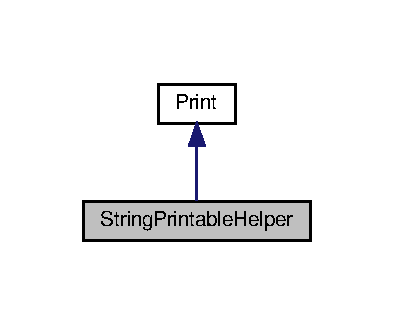
\includegraphics[width=189pt]{class_string_printable_helper__inherit__graph}
\end{center}
\end{figure}


Collaboration diagram for String\+Printable\+Helper\+:\nopagebreak
\begin{figure}[H]
\begin{center}
\leavevmode
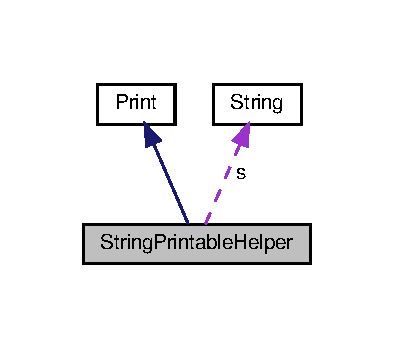
\includegraphics[width=189pt]{class_string_printable_helper__coll__graph}
\end{center}
\end{figure}
\subsection*{Public Member Functions}
\begin{DoxyCompactItemize}
\item 
\textbf{ String\+Printable\+Helper} (\textbf{ String} \&s\+\_\+)
\item 
virtual size\+\_\+t \textbf{ write} (const uint8\+\_\+t $\ast$buffer, size\+\_\+t size) override
\item 
virtual size\+\_\+t \textbf{ write} (uint8\+\_\+t c) override
\end{DoxyCompactItemize}
\subsection*{Private Attributes}
\begin{DoxyCompactItemize}
\item 
\textbf{ String} \& \textbf{ s}
\end{DoxyCompactItemize}
\subsection*{Additional Inherited Members}


\subsection{Detailed Description}


Definition at line 757 of file spark\+\_\+wiring\+\_\+string.\+cpp.



\subsection{Constructor \& Destructor Documentation}
\mbox{\label{class_string_printable_helper_aee189f4d6b8a240ba9c0f69674e94fc7}} 
\index{String\+Printable\+Helper@{String\+Printable\+Helper}!String\+Printable\+Helper@{String\+Printable\+Helper}}
\index{String\+Printable\+Helper@{String\+Printable\+Helper}!String\+Printable\+Helper@{String\+Printable\+Helper}}
\subsubsection{String\+Printable\+Helper()}
{\footnotesize\ttfamily String\+Printable\+Helper\+::\+String\+Printable\+Helper (\begin{DoxyParamCaption}\item[{\textbf{ String} \&}]{s\+\_\+ }\end{DoxyParamCaption})\hspace{0.3cm}{\ttfamily [inline]}}



Definition at line 763 of file spark\+\_\+wiring\+\_\+string.\+cpp.



References String\+::reserve(), and s.



Referenced by String\+::\+String().


\begin{DoxyCode}
763                                       : s(s\_) \{
764         s.reserve(20);
765     \}
\end{DoxyCode}


\subsection{Member Function Documentation}
\mbox{\label{class_string_printable_helper_a8098bfb565b518cec0cf9e6fbc68eed8}} 
\index{String\+Printable\+Helper@{String\+Printable\+Helper}!write@{write}}
\index{write@{write}!String\+Printable\+Helper@{String\+Printable\+Helper}}
\subsubsection{write()\hspace{0.1cm}{\footnotesize\ttfamily [1/2]}}
{\footnotesize\ttfamily virtual size\+\_\+t String\+Printable\+Helper\+::write (\begin{DoxyParamCaption}\item[{const uint8\+\_\+t $\ast$}]{buffer,  }\item[{size\+\_\+t}]{size }\end{DoxyParamCaption})\hspace{0.3cm}{\ttfamily [inline]}, {\ttfamily [override]}, {\ttfamily [virtual]}}



Reimplemented from \textbf{ Print} \doxyref{}{p.}{class_print_ad98d820df11e2697be1e4b1ea30b4a23}.



Definition at line 767 of file spark\+\_\+wiring\+\_\+string.\+cpp.



References String\+::concat(), String\+::length(), and s.


\begin{DoxyCode}
768     \{
769         \textcolor{keywordtype}{unsigned} len = s.length();
770         s.concat((\textcolor{keyword}{const} \textcolor{keywordtype}{char}*)buffer, size);
771         \textcolor{keywordflow}{return} s.length()-len;
772     \}
\end{DoxyCode}
\mbox{\label{class_string_printable_helper_adc5aab11289f917cefa1225b59afde2a}} 
\index{String\+Printable\+Helper@{String\+Printable\+Helper}!write@{write}}
\index{write@{write}!String\+Printable\+Helper@{String\+Printable\+Helper}}
\subsubsection{write()\hspace{0.1cm}{\footnotesize\ttfamily [2/2]}}
{\footnotesize\ttfamily virtual size\+\_\+t String\+Printable\+Helper\+::write (\begin{DoxyParamCaption}\item[{uint8\+\_\+t}]{c }\end{DoxyParamCaption})\hspace{0.3cm}{\ttfamily [inline]}, {\ttfamily [override]}, {\ttfamily [virtual]}}



Implements \textbf{ Print} \doxyref{}{p.}{class_print_a5be30d49adae2406a270c29ba9a3e0a3}.



Definition at line 774 of file spark\+\_\+wiring\+\_\+string.\+cpp.



References String\+::concat(), and s.


\begin{DoxyCode}
775     \{
776         \textcolor{keywordflow}{return} s.concat((\textcolor{keywordtype}{char})c);
777     \}
\end{DoxyCode}


\subsection{Member Data Documentation}
\mbox{\label{class_string_printable_helper_ac8273d5d460215114d9db27d7c7cab2e}} 
\index{String\+Printable\+Helper@{String\+Printable\+Helper}!s@{s}}
\index{s@{s}!String\+Printable\+Helper@{String\+Printable\+Helper}}
\subsubsection{s}
{\footnotesize\ttfamily \textbf{ String}\& String\+Printable\+Helper\+::s\hspace{0.3cm}{\ttfamily [private]}}



Definition at line 759 of file spark\+\_\+wiring\+\_\+string.\+cpp.



Referenced by String\+Printable\+Helper(), and write().



The documentation for this class was generated from the following file\+:\begin{DoxyCompactItemize}
\item 
lib/\+Json\+Parser\+Generator\+R\+K/test/gcclib/\textbf{ spark\+\_\+wiring\+\_\+string.\+cpp}\end{DoxyCompactItemize}

\hypertarget{class_string_sum_helper}{}\section{String\+Sum\+Helper Class Reference}
\label{class_string_sum_helper}\index{String\+Sum\+Helper@{String\+Sum\+Helper}}


Class used when appending mutiple \hyperlink{class_string}{String} and other values using +.  




{\ttfamily \#include $<$spark\+\_\+wiring\+\_\+string.\+h$>$}



Inheritance diagram for String\+Sum\+Helper\+:\nopagebreak
\begin{figure}[H]
\begin{center}
\leavevmode
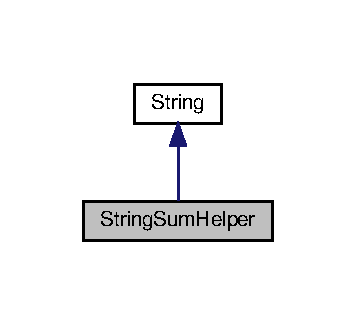
\includegraphics[width=171pt]{class_string_sum_helper__inherit__graph}
\end{center}
\end{figure}


Collaboration diagram for String\+Sum\+Helper\+:\nopagebreak
\begin{figure}[H]
\begin{center}
\leavevmode
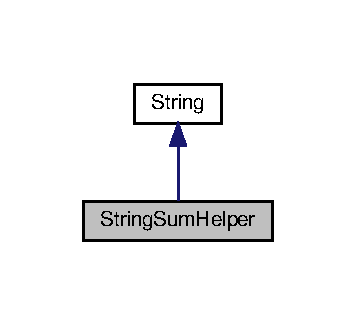
\includegraphics[width=171pt]{class_string_sum_helper__coll__graph}
\end{center}
\end{figure}
\subsection*{Public Member Functions}
\begin{DoxyCompactItemize}
\item 
\hyperlink{class_string_sum_helper_ae7676b662b830bbc8731f8b72f9413bb}{String\+Sum\+Helper} (const \hyperlink{class_string}{String} \&s)
\begin{DoxyCompactList}\small\item\em Append a \hyperlink{class_string}{String} object. \end{DoxyCompactList}\item 
\hyperlink{class_string_sum_helper_a73893e195336a0bcea77b16f4b35b422}{String\+Sum\+Helper} (const char $\ast$p)
\begin{DoxyCompactList}\small\item\em Append a const char $\ast$ (c-\/string, null terminated) \end{DoxyCompactList}\item 
\hyperlink{class_string_sum_helper_a529d5741ae2d4afeaa3068bff4f3b599}{String\+Sum\+Helper} (char c)
\begin{DoxyCompactList}\small\item\em Append a single character. \end{DoxyCompactList}\item 
\hyperlink{class_string_sum_helper_ac8f1e6c222659795a6aca08ad0872bec}{String\+Sum\+Helper} (unsigned char num)
\begin{DoxyCompactList}\small\item\em Append a byte as a decimal number 0 -\/ 255. \end{DoxyCompactList}\item 
\hyperlink{class_string_sum_helper_acb28b89b1f39f1140ab097439c967e22}{String\+Sum\+Helper} (int num)
\begin{DoxyCompactList}\small\item\em Append a 32-\/bit signed integer as a decimal number. \end{DoxyCompactList}\item 
\hyperlink{class_string_sum_helper_a13f4d006d1f67d0d2556152f4d16e4e9}{String\+Sum\+Helper} (unsigned int num)
\begin{DoxyCompactList}\small\item\em Append a 32-\/bit unsigned integer as a decimal number. \end{DoxyCompactList}\item 
\hyperlink{class_string_sum_helper_a6fefb0b3145abdc5632134a41770eaf7}{String\+Sum\+Helper} (long num)
\begin{DoxyCompactList}\small\item\em Append a 32-\/bit long integer as a decimal number. \end{DoxyCompactList}\item 
\hyperlink{class_string_sum_helper_ad05bd49f0b730d78d0a5dcf1b8c512eb}{String\+Sum\+Helper} (unsigned long num)
\begin{DoxyCompactList}\small\item\em Append a 32-\/bit unsigned long as a decimal number. \end{DoxyCompactList}\end{DoxyCompactItemize}
\subsection*{Additional Inherited Members}


\subsection{Detailed Description}
Class used when appending mutiple \hyperlink{class_string}{String} and other values using +. 

Definition at line 1085 of file spark\+\_\+wiring\+\_\+string.\+h.



\subsection{Constructor \& Destructor Documentation}
\mbox{\Hypertarget{class_string_sum_helper_ae7676b662b830bbc8731f8b72f9413bb}\label{class_string_sum_helper_ae7676b662b830bbc8731f8b72f9413bb}} 
\index{String\+Sum\+Helper@{String\+Sum\+Helper}!String\+Sum\+Helper@{String\+Sum\+Helper}}
\index{String\+Sum\+Helper@{String\+Sum\+Helper}!String\+Sum\+Helper@{String\+Sum\+Helper}}
\subsubsection{\texorpdfstring{String\+Sum\+Helper()}{StringSumHelper()}\hspace{0.1cm}{\footnotesize\ttfamily [1/8]}}
{\footnotesize\ttfamily String\+Sum\+Helper\+::\+String\+Sum\+Helper (\begin{DoxyParamCaption}\item[{const \hyperlink{class_string}{String} \&}]{s }\end{DoxyParamCaption})\hspace{0.3cm}{\ttfamily [inline]}}



Append a \hyperlink{class_string}{String} object. 


\begin{DoxyParams}{Parameters}
{\em s} & The string to append.\\
\hline
\end{DoxyParams}
\begin{DoxyReturn}{Returns}
\hyperlink{class_string_sum_helper}{String\+Sum\+Helper} object that encapsulates a copy of that string for appending to another string. 
\end{DoxyReturn}


Definition at line 1095 of file spark\+\_\+wiring\+\_\+string.\+h.



References String\+::\+String().

\mbox{\Hypertarget{class_string_sum_helper_a73893e195336a0bcea77b16f4b35b422}\label{class_string_sum_helper_a73893e195336a0bcea77b16f4b35b422}} 
\index{String\+Sum\+Helper@{String\+Sum\+Helper}!String\+Sum\+Helper@{String\+Sum\+Helper}}
\index{String\+Sum\+Helper@{String\+Sum\+Helper}!String\+Sum\+Helper@{String\+Sum\+Helper}}
\subsubsection{\texorpdfstring{String\+Sum\+Helper()}{StringSumHelper()}\hspace{0.1cm}{\footnotesize\ttfamily [2/8]}}
{\footnotesize\ttfamily String\+Sum\+Helper\+::\+String\+Sum\+Helper (\begin{DoxyParamCaption}\item[{const char $\ast$}]{p }\end{DoxyParamCaption})\hspace{0.3cm}{\ttfamily [inline]}}



Append a const char $\ast$ (c-\/string, null terminated) 


\begin{DoxyParams}{Parameters}
{\em p} & The string to append.\\
\hline
\end{DoxyParams}
\begin{DoxyReturn}{Returns}
\hyperlink{class_string_sum_helper}{String\+Sum\+Helper} object that encapsulates a copy of that string for appending to another string. 
\end{DoxyReturn}


Definition at line 1104 of file spark\+\_\+wiring\+\_\+string.\+h.



References String\+::\+String().

\mbox{\Hypertarget{class_string_sum_helper_a529d5741ae2d4afeaa3068bff4f3b599}\label{class_string_sum_helper_a529d5741ae2d4afeaa3068bff4f3b599}} 
\index{String\+Sum\+Helper@{String\+Sum\+Helper}!String\+Sum\+Helper@{String\+Sum\+Helper}}
\index{String\+Sum\+Helper@{String\+Sum\+Helper}!String\+Sum\+Helper@{String\+Sum\+Helper}}
\subsubsection{\texorpdfstring{String\+Sum\+Helper()}{StringSumHelper()}\hspace{0.1cm}{\footnotesize\ttfamily [3/8]}}
{\footnotesize\ttfamily String\+Sum\+Helper\+::\+String\+Sum\+Helper (\begin{DoxyParamCaption}\item[{char}]{c }\end{DoxyParamCaption})\hspace{0.3cm}{\ttfamily [inline]}}



Append a single character. 


\begin{DoxyParams}{Parameters}
{\em c} & The character to append.\\
\hline
\end{DoxyParams}
\begin{DoxyReturn}{Returns}
\hyperlink{class_string_sum_helper}{String\+Sum\+Helper} object that encapsulates a copy of that character for appending to another string. 
\end{DoxyReturn}


Definition at line 1113 of file spark\+\_\+wiring\+\_\+string.\+h.



References String\+::\+String().

\mbox{\Hypertarget{class_string_sum_helper_ac8f1e6c222659795a6aca08ad0872bec}\label{class_string_sum_helper_ac8f1e6c222659795a6aca08ad0872bec}} 
\index{String\+Sum\+Helper@{String\+Sum\+Helper}!String\+Sum\+Helper@{String\+Sum\+Helper}}
\index{String\+Sum\+Helper@{String\+Sum\+Helper}!String\+Sum\+Helper@{String\+Sum\+Helper}}
\subsubsection{\texorpdfstring{String\+Sum\+Helper()}{StringSumHelper()}\hspace{0.1cm}{\footnotesize\ttfamily [4/8]}}
{\footnotesize\ttfamily String\+Sum\+Helper\+::\+String\+Sum\+Helper (\begin{DoxyParamCaption}\item[{unsigned char}]{num }\end{DoxyParamCaption})\hspace{0.3cm}{\ttfamily [inline]}}



Append a byte as a decimal number 0 -\/ 255. 


\begin{DoxyParams}{Parameters}
{\em num} & The byte value to append.\\
\hline
\end{DoxyParams}
\begin{DoxyReturn}{Returns}
\hyperlink{class_string_sum_helper}{String\+Sum\+Helper} object that encapsulates the textual representation of the number for appending to another string. 
\end{DoxyReturn}


Definition at line 1122 of file spark\+\_\+wiring\+\_\+string.\+h.



References String\+::\+String().

\mbox{\Hypertarget{class_string_sum_helper_acb28b89b1f39f1140ab097439c967e22}\label{class_string_sum_helper_acb28b89b1f39f1140ab097439c967e22}} 
\index{String\+Sum\+Helper@{String\+Sum\+Helper}!String\+Sum\+Helper@{String\+Sum\+Helper}}
\index{String\+Sum\+Helper@{String\+Sum\+Helper}!String\+Sum\+Helper@{String\+Sum\+Helper}}
\subsubsection{\texorpdfstring{String\+Sum\+Helper()}{StringSumHelper()}\hspace{0.1cm}{\footnotesize\ttfamily [5/8]}}
{\footnotesize\ttfamily String\+Sum\+Helper\+::\+String\+Sum\+Helper (\begin{DoxyParamCaption}\item[{int}]{num }\end{DoxyParamCaption})\hspace{0.3cm}{\ttfamily [inline]}}



Append a 32-\/bit signed integer as a decimal number. 


\begin{DoxyParams}{Parameters}
{\em num} & The byte value to append.\\
\hline
\end{DoxyParams}
\begin{DoxyReturn}{Returns}
\hyperlink{class_string_sum_helper}{String\+Sum\+Helper} object that encapsulates the textual representation of the number for appending to another string. 
\end{DoxyReturn}


Definition at line 1131 of file spark\+\_\+wiring\+\_\+string.\+h.



References String\+::\+String().

\mbox{\Hypertarget{class_string_sum_helper_a13f4d006d1f67d0d2556152f4d16e4e9}\label{class_string_sum_helper_a13f4d006d1f67d0d2556152f4d16e4e9}} 
\index{String\+Sum\+Helper@{String\+Sum\+Helper}!String\+Sum\+Helper@{String\+Sum\+Helper}}
\index{String\+Sum\+Helper@{String\+Sum\+Helper}!String\+Sum\+Helper@{String\+Sum\+Helper}}
\subsubsection{\texorpdfstring{String\+Sum\+Helper()}{StringSumHelper()}\hspace{0.1cm}{\footnotesize\ttfamily [6/8]}}
{\footnotesize\ttfamily String\+Sum\+Helper\+::\+String\+Sum\+Helper (\begin{DoxyParamCaption}\item[{unsigned int}]{num }\end{DoxyParamCaption})\hspace{0.3cm}{\ttfamily [inline]}}



Append a 32-\/bit unsigned integer as a decimal number. 


\begin{DoxyParams}{Parameters}
{\em num} & The byte value to append.\\
\hline
\end{DoxyParams}
\begin{DoxyReturn}{Returns}
\hyperlink{class_string_sum_helper}{String\+Sum\+Helper} object that encapsulates the textual representation of the number for appending to another string. 
\end{DoxyReturn}


Definition at line 1140 of file spark\+\_\+wiring\+\_\+string.\+h.



References String\+::\+String().

\mbox{\Hypertarget{class_string_sum_helper_a6fefb0b3145abdc5632134a41770eaf7}\label{class_string_sum_helper_a6fefb0b3145abdc5632134a41770eaf7}} 
\index{String\+Sum\+Helper@{String\+Sum\+Helper}!String\+Sum\+Helper@{String\+Sum\+Helper}}
\index{String\+Sum\+Helper@{String\+Sum\+Helper}!String\+Sum\+Helper@{String\+Sum\+Helper}}
\subsubsection{\texorpdfstring{String\+Sum\+Helper()}{StringSumHelper()}\hspace{0.1cm}{\footnotesize\ttfamily [7/8]}}
{\footnotesize\ttfamily String\+Sum\+Helper\+::\+String\+Sum\+Helper (\begin{DoxyParamCaption}\item[{long}]{num }\end{DoxyParamCaption})\hspace{0.3cm}{\ttfamily [inline]}}



Append a 32-\/bit long integer as a decimal number. 


\begin{DoxyParams}{Parameters}
{\em num} & The byte value to append.\\
\hline
\end{DoxyParams}
\begin{DoxyReturn}{Returns}
\hyperlink{class_string_sum_helper}{String\+Sum\+Helper} object that encapsulates the textual representation of the number for appending to another string. 
\end{DoxyReturn}


Definition at line 1149 of file spark\+\_\+wiring\+\_\+string.\+h.



References String\+::\+String().

\mbox{\Hypertarget{class_string_sum_helper_ad05bd49f0b730d78d0a5dcf1b8c512eb}\label{class_string_sum_helper_ad05bd49f0b730d78d0a5dcf1b8c512eb}} 
\index{String\+Sum\+Helper@{String\+Sum\+Helper}!String\+Sum\+Helper@{String\+Sum\+Helper}}
\index{String\+Sum\+Helper@{String\+Sum\+Helper}!String\+Sum\+Helper@{String\+Sum\+Helper}}
\subsubsection{\texorpdfstring{String\+Sum\+Helper()}{StringSumHelper()}\hspace{0.1cm}{\footnotesize\ttfamily [8/8]}}
{\footnotesize\ttfamily String\+Sum\+Helper\+::\+String\+Sum\+Helper (\begin{DoxyParamCaption}\item[{unsigned long}]{num }\end{DoxyParamCaption})\hspace{0.3cm}{\ttfamily [inline]}}



Append a 32-\/bit unsigned long as a decimal number. 


\begin{DoxyParams}{Parameters}
{\em num} & The byte value to append.\\
\hline
\end{DoxyParams}
\begin{DoxyReturn}{Returns}
\hyperlink{class_string_sum_helper}{String\+Sum\+Helper} object that encapsulates the textual representation of the number for appending to another string. 
\end{DoxyReturn}


Definition at line 1158 of file spark\+\_\+wiring\+\_\+string.\+h.



References String\+::\+String().



The documentation for this class was generated from the following file\+:\begin{DoxyCompactItemize}
\item 
lib/\+Json\+Parser\+Generator\+R\+K/docs/src/\hyperlink{docs_2src_2spark__wiring__string_8h}{spark\+\_\+wiring\+\_\+string.\+h}\end{DoxyCompactItemize}

\section{M\+F\+R\+C522\+:\+:Uid Struct Reference}
\label{struct_m_f_r_c522_1_1_uid}\index{M\+F\+R\+C522\+::\+Uid@{M\+F\+R\+C522\+::\+Uid}}


{\ttfamily \#include $<$M\+F\+R\+C522.\+h$>$}

\subsection*{Public Attributes}
\begin{DoxyCompactItemize}
\item 
byte \textbf{ size}
\item 
byte \textbf{ uid\+Byte} [10]
\item 
byte \textbf{ sak}
\end{DoxyCompactItemize}


\subsection{Detailed Description}


Definition at line 254 of file M\+F\+R\+C522.\+h.



\subsection{Member Data Documentation}
\mbox{\label{struct_m_f_r_c522_1_1_uid_a90aa2fd57a03011252148c2ccdc8875b}} 
\index{M\+F\+R\+C522\+::\+Uid@{M\+F\+R\+C522\+::\+Uid}!sak@{sak}}
\index{sak@{sak}!M\+F\+R\+C522\+::\+Uid@{M\+F\+R\+C522\+::\+Uid}}
\subsubsection{sak}
{\footnotesize\ttfamily byte M\+F\+R\+C522\+::\+Uid\+::sak}



Definition at line 257 of file M\+F\+R\+C522.\+h.

\mbox{\label{struct_m_f_r_c522_1_1_uid_a49c06f93c7748abe00a9ab5899d479b7}} 
\index{M\+F\+R\+C522\+::\+Uid@{M\+F\+R\+C522\+::\+Uid}!size@{size}}
\index{size@{size}!M\+F\+R\+C522\+::\+Uid@{M\+F\+R\+C522\+::\+Uid}}
\subsubsection{size}
{\footnotesize\ttfamily byte M\+F\+R\+C522\+::\+Uid\+::size}



Definition at line 255 of file M\+F\+R\+C522.\+h.

\mbox{\label{struct_m_f_r_c522_1_1_uid_a5581167c1e1c8beb98c44ff86f4fbc52}} 
\index{M\+F\+R\+C522\+::\+Uid@{M\+F\+R\+C522\+::\+Uid}!uid\+Byte@{uid\+Byte}}
\index{uid\+Byte@{uid\+Byte}!M\+F\+R\+C522\+::\+Uid@{M\+F\+R\+C522\+::\+Uid}}
\subsubsection{uid\+Byte}
{\footnotesize\ttfamily byte M\+F\+R\+C522\+::\+Uid\+::uid\+Byte[10]}



Definition at line 256 of file M\+F\+R\+C522.\+h.



The documentation for this struct was generated from the following file\+:\begin{DoxyCompactItemize}
\item 
lib/\+M\+F\+R\+C522/src/\textbf{ M\+F\+R\+C522.\+h}\end{DoxyCompactItemize}

\chapter{File Documentation}
\hypertarget{docs_2src_2spark__wiring__print_8h}{}\section{lib/\+Json\+Parser\+Generator\+R\+K/docs/src/spark\+\_\+wiring\+\_\+print.h File Reference}
\label{docs_2src_2spark__wiring__print_8h}\index{lib/\+Json\+Parser\+Generator\+R\+K/docs/src/spark\+\_\+wiring\+\_\+print.\+h@{lib/\+Json\+Parser\+Generator\+R\+K/docs/src/spark\+\_\+wiring\+\_\+print.\+h}}
{\ttfamily \#include $<$stddef.\+h$>$}\newline
{\ttfamily \#include $<$string.\+h$>$}\newline
{\ttfamily \#include $<$stdint.\+h$>$}\newline
{\ttfamily \#include \char`\"{}spark\+\_\+wiring\+\_\+string.\+h\char`\"{}}\newline
{\ttfamily \#include \char`\"{}spark\+\_\+wiring\+\_\+printable.\+h\char`\"{}}\newline
Include dependency graph for spark\+\_\+wiring\+\_\+print.\+h\+:
\nopagebreak
\begin{figure}[H]
\begin{center}
\leavevmode
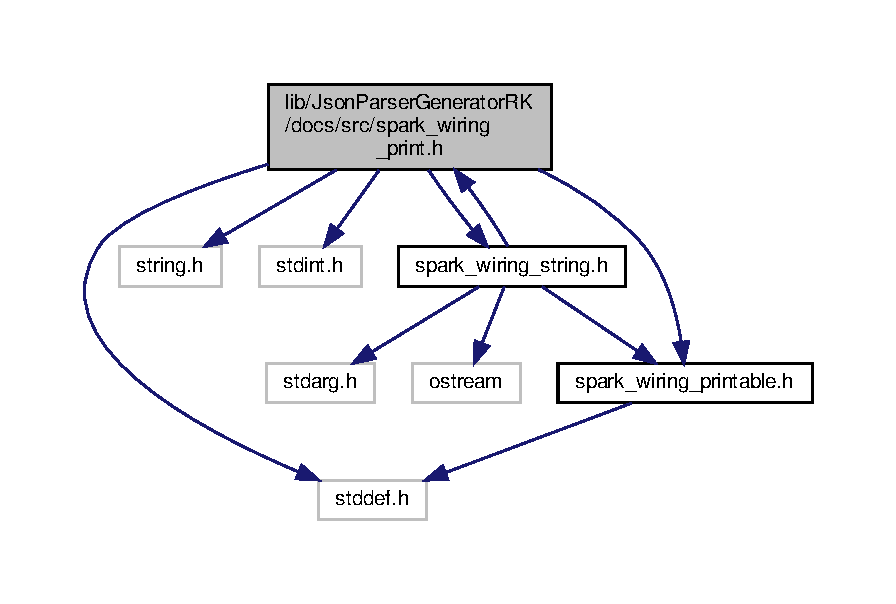
\includegraphics[width=350pt]{docs_2src_2spark__wiring__print_8h__incl}
\end{center}
\end{figure}
This graph shows which files directly or indirectly include this file\+:
\nopagebreak
\begin{figure}[H]
\begin{center}
\leavevmode
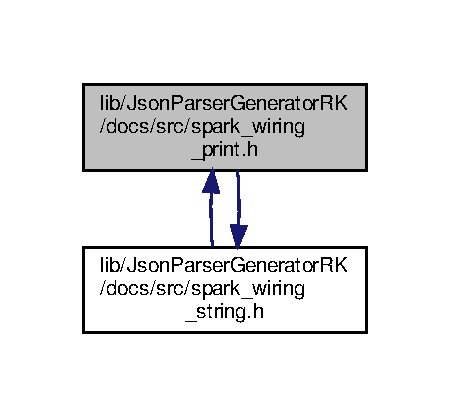
\includegraphics[width=216pt]{docs_2src_2spark__wiring__print_8h__dep__incl}
\end{center}
\end{figure}
\subsection*{Classes}
\begin{DoxyCompactItemize}
\item 
class \hyperlink{class_print}{Print}
\begin{DoxyCompactList}\small\item\em Class for printing to a stream or file. \end{DoxyCompactList}\end{DoxyCompactItemize}
\subsection*{Macros}
\begin{DoxyCompactItemize}
\item 
\#define \hyperlink{docs_2src_2spark__wiring__print_8h_a31cf2682ae26587a3c76b612b6d05337}{\+\_\+\+\_\+\+S\+P\+A\+R\+K\+\_\+\+W\+I\+R\+I\+N\+G\+\_\+\+P\+R\+I\+N\+T\+\_\+}
\end{DoxyCompactItemize}
\subsection*{Variables}
\begin{DoxyCompactItemize}
\item 
const unsigned char \hyperlink{docs_2src_2spark__wiring__print_8h_a26e216c38cffa0a9965fa7933ba558b1}{D\+EC} = 10
\begin{DoxyCompactList}\small\item\em Decimal number format (0-\/9) \end{DoxyCompactList}\item 
const unsigned char \hyperlink{docs_2src_2spark__wiring__print_8h_a777726851dda95dabcc50f606e2dfd8e}{H\+EX} = 16
\begin{DoxyCompactList}\small\item\em Hexadecimal number format (0-\/9, a-\/f) \end{DoxyCompactList}\item 
const unsigned char \hyperlink{docs_2src_2spark__wiring__print_8h_aeea5c9efade0b29d08f3b5b8336425ad}{O\+CT} = 8
\begin{DoxyCompactList}\small\item\em Octal number format (0-\/7) \end{DoxyCompactList}\item 
const unsigned char \hyperlink{docs_2src_2spark__wiring__print_8h_aee179d58d1b76a9b42397af886f2f9a4}{B\+IN} = 2
\begin{DoxyCompactList}\small\item\em Binary number format (0-\/1) \end{DoxyCompactList}\end{DoxyCompactItemize}


\subsection{Macro Definition Documentation}
\mbox{\Hypertarget{docs_2src_2spark__wiring__print_8h_a31cf2682ae26587a3c76b612b6d05337}\label{docs_2src_2spark__wiring__print_8h_a31cf2682ae26587a3c76b612b6d05337}} 
\index{docs/src/spark\+\_\+wiring\+\_\+print.\+h@{docs/src/spark\+\_\+wiring\+\_\+print.\+h}!\+\_\+\+\_\+\+S\+P\+A\+R\+K\+\_\+\+W\+I\+R\+I\+N\+G\+\_\+\+P\+R\+I\+N\+T\+\_\+@{\+\_\+\+\_\+\+S\+P\+A\+R\+K\+\_\+\+W\+I\+R\+I\+N\+G\+\_\+\+P\+R\+I\+N\+T\+\_\+}}
\index{\+\_\+\+\_\+\+S\+P\+A\+R\+K\+\_\+\+W\+I\+R\+I\+N\+G\+\_\+\+P\+R\+I\+N\+T\+\_\+@{\+\_\+\+\_\+\+S\+P\+A\+R\+K\+\_\+\+W\+I\+R\+I\+N\+G\+\_\+\+P\+R\+I\+N\+T\+\_\+}!docs/src/spark\+\_\+wiring\+\_\+print.\+h@{docs/src/spark\+\_\+wiring\+\_\+print.\+h}}
\subsubsection{\texorpdfstring{\+\_\+\+\_\+\+S\+P\+A\+R\+K\+\_\+\+W\+I\+R\+I\+N\+G\+\_\+\+P\+R\+I\+N\+T\+\_\+}{\_\_SPARK\_WIRING\_PRINT\_}}
{\footnotesize\ttfamily \#define \+\_\+\+\_\+\+S\+P\+A\+R\+K\+\_\+\+W\+I\+R\+I\+N\+G\+\_\+\+P\+R\+I\+N\+T\+\_\+}



Definition at line 28 of file spark\+\_\+wiring\+\_\+print.\+h.



\subsection{Variable Documentation}
\mbox{\Hypertarget{docs_2src_2spark__wiring__print_8h_aee179d58d1b76a9b42397af886f2f9a4}\label{docs_2src_2spark__wiring__print_8h_aee179d58d1b76a9b42397af886f2f9a4}} 
\index{docs/src/spark\+\_\+wiring\+\_\+print.\+h@{docs/src/spark\+\_\+wiring\+\_\+print.\+h}!B\+IN@{B\+IN}}
\index{B\+IN@{B\+IN}!docs/src/spark\+\_\+wiring\+\_\+print.\+h@{docs/src/spark\+\_\+wiring\+\_\+print.\+h}}
\subsubsection{\texorpdfstring{B\+IN}{BIN}}
{\footnotesize\ttfamily const unsigned char B\+IN = 2}



Binary number format (0-\/1) 



Definition at line 40 of file spark\+\_\+wiring\+\_\+print.\+h.

\mbox{\Hypertarget{docs_2src_2spark__wiring__print_8h_a26e216c38cffa0a9965fa7933ba558b1}\label{docs_2src_2spark__wiring__print_8h_a26e216c38cffa0a9965fa7933ba558b1}} 
\index{docs/src/spark\+\_\+wiring\+\_\+print.\+h@{docs/src/spark\+\_\+wiring\+\_\+print.\+h}!D\+EC@{D\+EC}}
\index{D\+EC@{D\+EC}!docs/src/spark\+\_\+wiring\+\_\+print.\+h@{docs/src/spark\+\_\+wiring\+\_\+print.\+h}}
\subsubsection{\texorpdfstring{D\+EC}{DEC}}
{\footnotesize\ttfamily const unsigned char D\+EC = 10}



Decimal number format (0-\/9) 



Definition at line 37 of file spark\+\_\+wiring\+\_\+print.\+h.



Referenced by String\+::concat().

\mbox{\Hypertarget{docs_2src_2spark__wiring__print_8h_a777726851dda95dabcc50f606e2dfd8e}\label{docs_2src_2spark__wiring__print_8h_a777726851dda95dabcc50f606e2dfd8e}} 
\index{docs/src/spark\+\_\+wiring\+\_\+print.\+h@{docs/src/spark\+\_\+wiring\+\_\+print.\+h}!H\+EX@{H\+EX}}
\index{H\+EX@{H\+EX}!docs/src/spark\+\_\+wiring\+\_\+print.\+h@{docs/src/spark\+\_\+wiring\+\_\+print.\+h}}
\subsubsection{\texorpdfstring{H\+EX}{HEX}}
{\footnotesize\ttfamily const unsigned char H\+EX = 16}



Hexadecimal number format (0-\/9, a-\/f) 



Definition at line 38 of file spark\+\_\+wiring\+\_\+print.\+h.

\mbox{\Hypertarget{docs_2src_2spark__wiring__print_8h_aeea5c9efade0b29d08f3b5b8336425ad}\label{docs_2src_2spark__wiring__print_8h_aeea5c9efade0b29d08f3b5b8336425ad}} 
\index{docs/src/spark\+\_\+wiring\+\_\+print.\+h@{docs/src/spark\+\_\+wiring\+\_\+print.\+h}!O\+CT@{O\+CT}}
\index{O\+CT@{O\+CT}!docs/src/spark\+\_\+wiring\+\_\+print.\+h@{docs/src/spark\+\_\+wiring\+\_\+print.\+h}}
\subsubsection{\texorpdfstring{O\+CT}{OCT}}
{\footnotesize\ttfamily const unsigned char O\+CT = 8}



Octal number format (0-\/7) 



Definition at line 39 of file spark\+\_\+wiring\+\_\+print.\+h.


\section{lib/\+Json\+Parser\+Generator\+R\+K/test/gcclib/spark\+\_\+wiring\+\_\+print.h File Reference}
\label{test_2gcclib_2spark__wiring__print_8h}\index{lib/\+Json\+Parser\+Generator\+R\+K/test/gcclib/spark\+\_\+wiring\+\_\+print.\+h@{lib/\+Json\+Parser\+Generator\+R\+K/test/gcclib/spark\+\_\+wiring\+\_\+print.\+h}}
{\ttfamily \#include $<$stddef.\+h$>$}\newline
{\ttfamily \#include $<$string.\+h$>$}\newline
{\ttfamily \#include $<$stdint.\+h$>$}\newline
{\ttfamily \#include \char`\"{}spark\+\_\+wiring\+\_\+string.\+h\char`\"{}}\newline
{\ttfamily \#include \char`\"{}spark\+\_\+wiring\+\_\+printable.\+h\char`\"{}}\newline
Include dependency graph for spark\+\_\+wiring\+\_\+print.\+h\+:\nopagebreak
\begin{figure}[H]
\begin{center}
\leavevmode
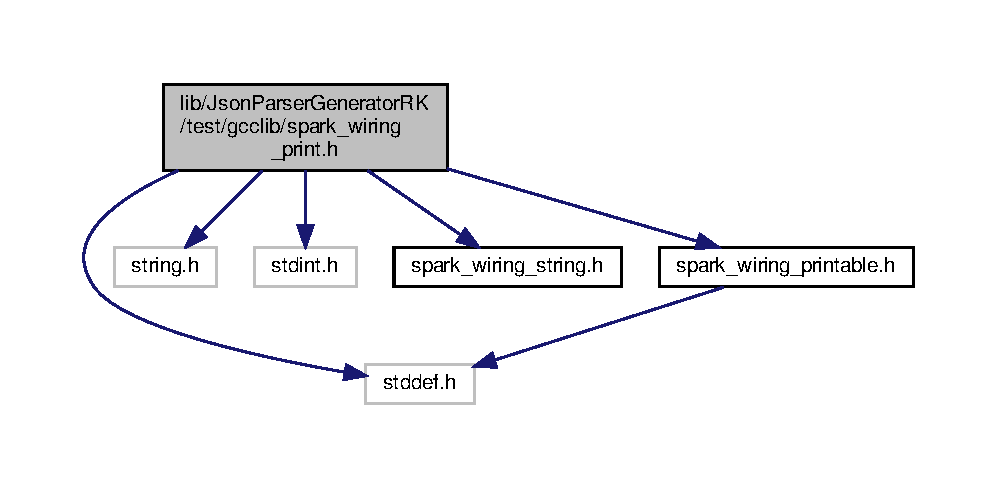
\includegraphics[width=350pt]{test_2gcclib_2spark__wiring__print_8h__incl}
\end{center}
\end{figure}
This graph shows which files directly or indirectly include this file\+:\nopagebreak
\begin{figure}[H]
\begin{center}
\leavevmode
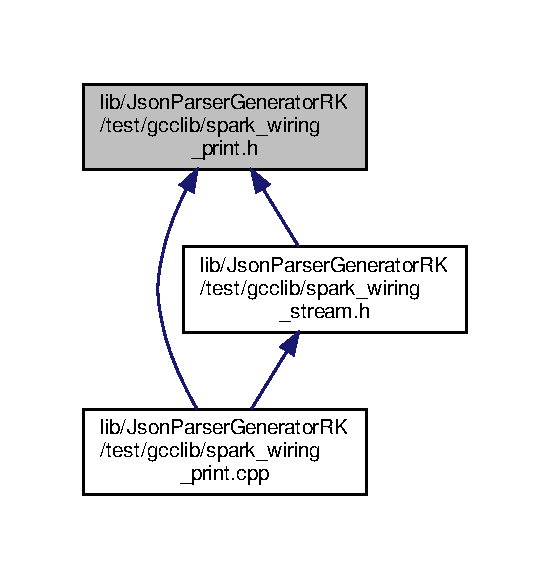
\includegraphics[width=264pt]{test_2gcclib_2spark__wiring__print_8h__dep__incl}
\end{center}
\end{figure}
\subsection*{Classes}
\begin{DoxyCompactItemize}
\item 
class \textbf{ Print}
\begin{DoxyCompactList}\small\item\em Class for printing to a stream or file. \end{DoxyCompactList}\end{DoxyCompactItemize}
\subsection*{Variables}
\begin{DoxyCompactItemize}
\item 
const unsigned char \textbf{ D\+EC} = 10
\item 
const unsigned char \textbf{ H\+EX} = 16
\item 
const unsigned char \textbf{ O\+CT} = 8
\item 
const unsigned char \textbf{ B\+IN} = 2
\end{DoxyCompactItemize}


\subsection{Variable Documentation}
\mbox{\label{test_2gcclib_2spark__wiring__print_8h_aee179d58d1b76a9b42397af886f2f9a4}} 
\index{test/gcclib/spark\+\_\+wiring\+\_\+print.\+h@{test/gcclib/spark\+\_\+wiring\+\_\+print.\+h}!B\+IN@{B\+IN}}
\index{B\+IN@{B\+IN}!test/gcclib/spark\+\_\+wiring\+\_\+print.\+h@{test/gcclib/spark\+\_\+wiring\+\_\+print.\+h}}
\subsubsection{B\+IN}
{\footnotesize\ttfamily const unsigned char B\+IN = 2}



Definition at line 40 of file spark\+\_\+wiring\+\_\+print.\+h.

\mbox{\label{test_2gcclib_2spark__wiring__print_8h_a26e216c38cffa0a9965fa7933ba558b1}} 
\index{test/gcclib/spark\+\_\+wiring\+\_\+print.\+h@{test/gcclib/spark\+\_\+wiring\+\_\+print.\+h}!D\+EC@{D\+EC}}
\index{D\+EC@{D\+EC}!test/gcclib/spark\+\_\+wiring\+\_\+print.\+h@{test/gcclib/spark\+\_\+wiring\+\_\+print.\+h}}
\subsubsection{D\+EC}
{\footnotesize\ttfamily const unsigned char D\+EC = 10}



Definition at line 37 of file spark\+\_\+wiring\+\_\+print.\+h.

\mbox{\label{test_2gcclib_2spark__wiring__print_8h_a777726851dda95dabcc50f606e2dfd8e}} 
\index{test/gcclib/spark\+\_\+wiring\+\_\+print.\+h@{test/gcclib/spark\+\_\+wiring\+\_\+print.\+h}!H\+EX@{H\+EX}}
\index{H\+EX@{H\+EX}!test/gcclib/spark\+\_\+wiring\+\_\+print.\+h@{test/gcclib/spark\+\_\+wiring\+\_\+print.\+h}}
\subsubsection{H\+EX}
{\footnotesize\ttfamily const unsigned char H\+EX = 16}



Definition at line 38 of file spark\+\_\+wiring\+\_\+print.\+h.

\mbox{\label{test_2gcclib_2spark__wiring__print_8h_aeea5c9efade0b29d08f3b5b8336425ad}} 
\index{test/gcclib/spark\+\_\+wiring\+\_\+print.\+h@{test/gcclib/spark\+\_\+wiring\+\_\+print.\+h}!O\+CT@{O\+CT}}
\index{O\+CT@{O\+CT}!test/gcclib/spark\+\_\+wiring\+\_\+print.\+h@{test/gcclib/spark\+\_\+wiring\+\_\+print.\+h}}
\subsubsection{O\+CT}
{\footnotesize\ttfamily const unsigned char O\+CT = 8}



Definition at line 39 of file spark\+\_\+wiring\+\_\+print.\+h.


\section{lib/\+Json\+Parser\+Generator\+R\+K/docs/src/spark\+\_\+wiring\+\_\+printable.h File Reference}
\label{docs_2src_2spark__wiring__printable_8h}\index{lib/\+Json\+Parser\+Generator\+R\+K/docs/src/spark\+\_\+wiring\+\_\+printable.\+h@{lib/\+Json\+Parser\+Generator\+R\+K/docs/src/spark\+\_\+wiring\+\_\+printable.\+h}}
{\ttfamily \#include $<$stddef.\+h$>$}\newline
Include dependency graph for spark\+\_\+wiring\+\_\+printable.\+h\+:\nopagebreak
\begin{figure}[H]
\begin{center}
\leavevmode
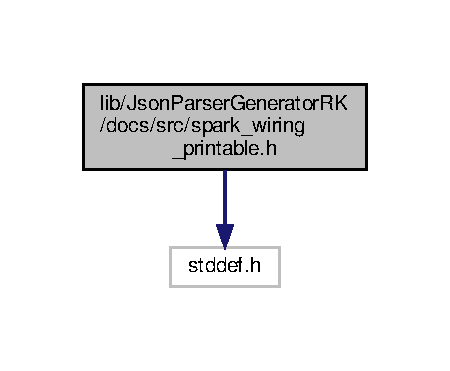
\includegraphics[width=216pt]{docs_2src_2spark__wiring__printable_8h__incl}
\end{center}
\end{figure}
This graph shows which files directly or indirectly include this file\+:\nopagebreak
\begin{figure}[H]
\begin{center}
\leavevmode
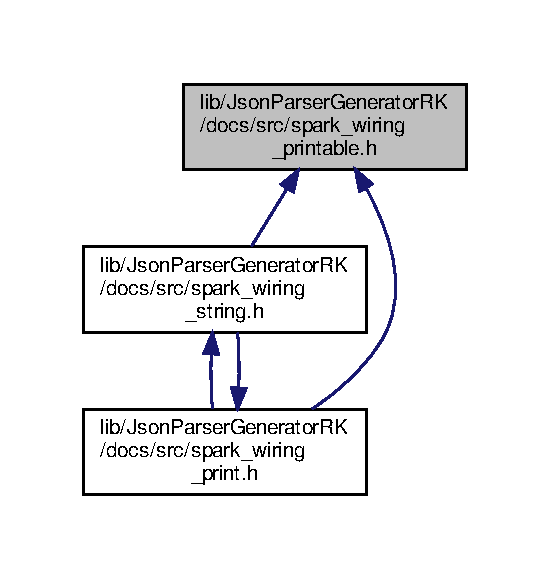
\includegraphics[width=264pt]{docs_2src_2spark__wiring__printable_8h__dep__incl}
\end{center}
\end{figure}
\subsection*{Classes}
\begin{DoxyCompactItemize}
\item 
class \textbf{ Printable}
\begin{DoxyCompactList}\small\item\em The \doxyref{Printable}{p.}{class_printable} class provides a way for new classes to allow themselves to be printed. \end{DoxyCompactList}\end{DoxyCompactItemize}

\hypertarget{test_2gcclib_2spark__wiring__printable_8h}{}\section{lib/\+Json\+Parser\+Generator\+R\+K/test/gcclib/spark\+\_\+wiring\+\_\+printable.h File Reference}
\label{test_2gcclib_2spark__wiring__printable_8h}\index{lib/\+Json\+Parser\+Generator\+R\+K/test/gcclib/spark\+\_\+wiring\+\_\+printable.\+h@{lib/\+Json\+Parser\+Generator\+R\+K/test/gcclib/spark\+\_\+wiring\+\_\+printable.\+h}}
{\ttfamily \#include $<$stddef.\+h$>$}\newline
Include dependency graph for spark\+\_\+wiring\+\_\+printable.\+h\+:
\nopagebreak
\begin{figure}[H]
\begin{center}
\leavevmode
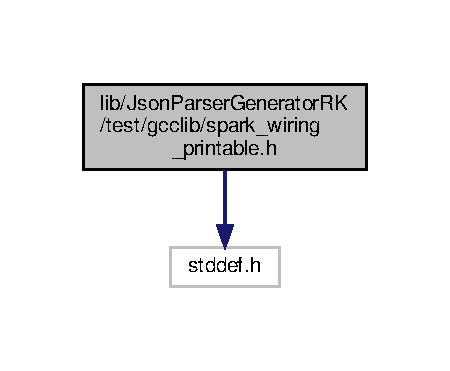
\includegraphics[width=216pt]{test_2gcclib_2spark__wiring__printable_8h__incl}
\end{center}
\end{figure}
This graph shows which files directly or indirectly include this file\+:
\nopagebreak
\begin{figure}[H]
\begin{center}
\leavevmode
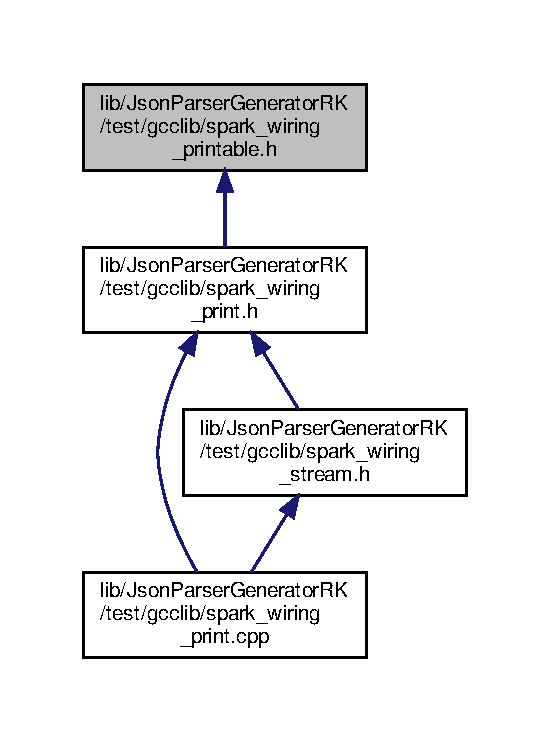
\includegraphics[width=264pt]{test_2gcclib_2spark__wiring__printable_8h__dep__incl}
\end{center}
\end{figure}
\subsection*{Classes}
\begin{DoxyCompactItemize}
\item 
class \hyperlink{class_printable}{Printable}
\begin{DoxyCompactList}\small\item\em The \hyperlink{class_printable}{Printable} class provides a way for new classes to allow themselves to be printed. \end{DoxyCompactList}\end{DoxyCompactItemize}

\section{lib/\+Json\+Parser\+Generator\+R\+K/docs/src/spark\+\_\+wiring\+\_\+string.h File Reference}
\label{docs_2src_2spark__wiring__string_8h}\index{lib/\+Json\+Parser\+Generator\+R\+K/docs/src/spark\+\_\+wiring\+\_\+string.\+h@{lib/\+Json\+Parser\+Generator\+R\+K/docs/src/spark\+\_\+wiring\+\_\+string.\+h}}
{\ttfamily \#include $<$stdarg.\+h$>$}\newline
{\ttfamily \#include \char`\"{}spark\+\_\+wiring\+\_\+print.\+h\char`\"{}}\newline
{\ttfamily \#include \char`\"{}spark\+\_\+wiring\+\_\+printable.\+h\char`\"{}}\newline
{\ttfamily \#include $<$ostream$>$}\newline
Include dependency graph for spark\+\_\+wiring\+\_\+string.\+h\+:\nopagebreak
\begin{figure}[H]
\begin{center}
\leavevmode
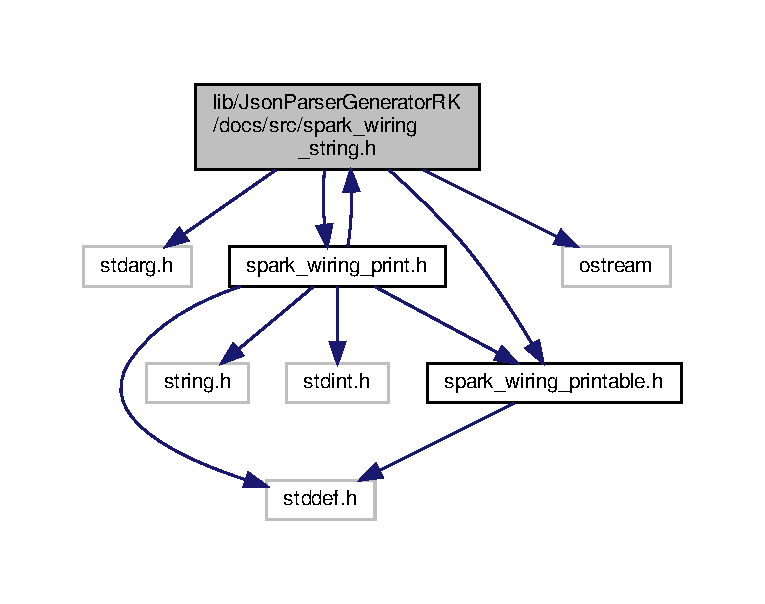
\includegraphics[width=350pt]{docs_2src_2spark__wiring__string_8h__incl}
\end{center}
\end{figure}
This graph shows which files directly or indirectly include this file\+:\nopagebreak
\begin{figure}[H]
\begin{center}
\leavevmode
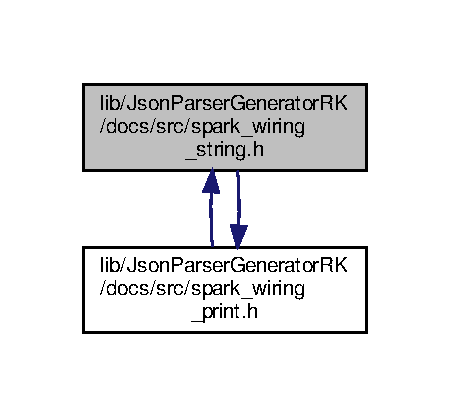
\includegraphics[width=216pt]{docs_2src_2spark__wiring__string_8h__dep__incl}
\end{center}
\end{figure}
\subsection*{Classes}
\begin{DoxyCompactItemize}
\item 
class \textbf{ String}
\begin{DoxyCompactList}\small\item\em Wiring \doxyref{String}{p.}{class_string}\+: A class to hold and manipulate a dynamically allocated string. \end{DoxyCompactList}\item 
class \textbf{ String\+Sum\+Helper}
\begin{DoxyCompactList}\small\item\em Class used when appending mutiple \doxyref{String}{p.}{class_string} and other values using +. \end{DoxyCompactList}\end{DoxyCompactItemize}
\subsection*{Macros}
\begin{DoxyCompactItemize}
\item 
\#define \textbf{ F}(X)~(X)
\end{DoxyCompactItemize}
\subsection*{Functions}
\begin{DoxyCompactItemize}
\item 
std\+::ostream \& \textbf{ operator$<$$<$} (std\+::ostream \&os, const \textbf{ String} \&value)
\end{DoxyCompactItemize}


\subsection{Macro Definition Documentation}
\mbox{\label{docs_2src_2spark__wiring__string_8h_a2ec9e0c82a2cc5b0eb0bc8158cc7d64c}} 
\index{docs/src/spark\+\_\+wiring\+\_\+string.\+h@{docs/src/spark\+\_\+wiring\+\_\+string.\+h}!F@{F}}
\index{F@{F}!docs/src/spark\+\_\+wiring\+\_\+string.\+h@{docs/src/spark\+\_\+wiring\+\_\+string.\+h}}
\subsubsection{F}
{\footnotesize\ttfamily \#define F(\begin{DoxyParamCaption}\item[{}]{X }\end{DoxyParamCaption})~(X)}



Definition at line 44 of file spark\+\_\+wiring\+\_\+string.\+h.



\subsection{Function Documentation}
\mbox{\label{docs_2src_2spark__wiring__string_8h_a75a6c2170b59dd7dc4b91f73f77d8e00}} 
\index{docs/src/spark\+\_\+wiring\+\_\+string.\+h@{docs/src/spark\+\_\+wiring\+\_\+string.\+h}!operator$<$$<$@{operator$<$$<$}}
\index{operator$<$$<$@{operator$<$$<$}!docs/src/spark\+\_\+wiring\+\_\+string.\+h@{docs/src/spark\+\_\+wiring\+\_\+string.\+h}}
\subsubsection{operator$<$$<$()}
{\footnotesize\ttfamily std\+::ostream\& operator$<$$<$ (\begin{DoxyParamCaption}\item[{std\+::ostream \&}]{os,  }\item[{const \textbf{ String} \&}]{value }\end{DoxyParamCaption})}



Definition at line 807 of file spark\+\_\+wiring\+\_\+string.\+cpp.



References String\+::c\+\_\+str().


\begin{DoxyCode}
807                                                                 \{
808     os << \textcolor{charliteral}{'"'} << value.c_str() << \textcolor{charliteral}{'"'};
809     \textcolor{keywordflow}{return} os;
810 \}
\end{DoxyCode}

\section{lib/\+Json\+Parser\+Generator\+R\+K/test/gcclib/spark\+\_\+wiring\+\_\+string.h File Reference}
\label{test_2gcclib_2spark__wiring__string_8h}\index{lib/\+Json\+Parser\+Generator\+R\+K/test/gcclib/spark\+\_\+wiring\+\_\+string.\+h@{lib/\+Json\+Parser\+Generator\+R\+K/test/gcclib/spark\+\_\+wiring\+\_\+string.\+h}}
This graph shows which files directly or indirectly include this file\+:\nopagebreak
\begin{figure}[H]
\begin{center}
\leavevmode
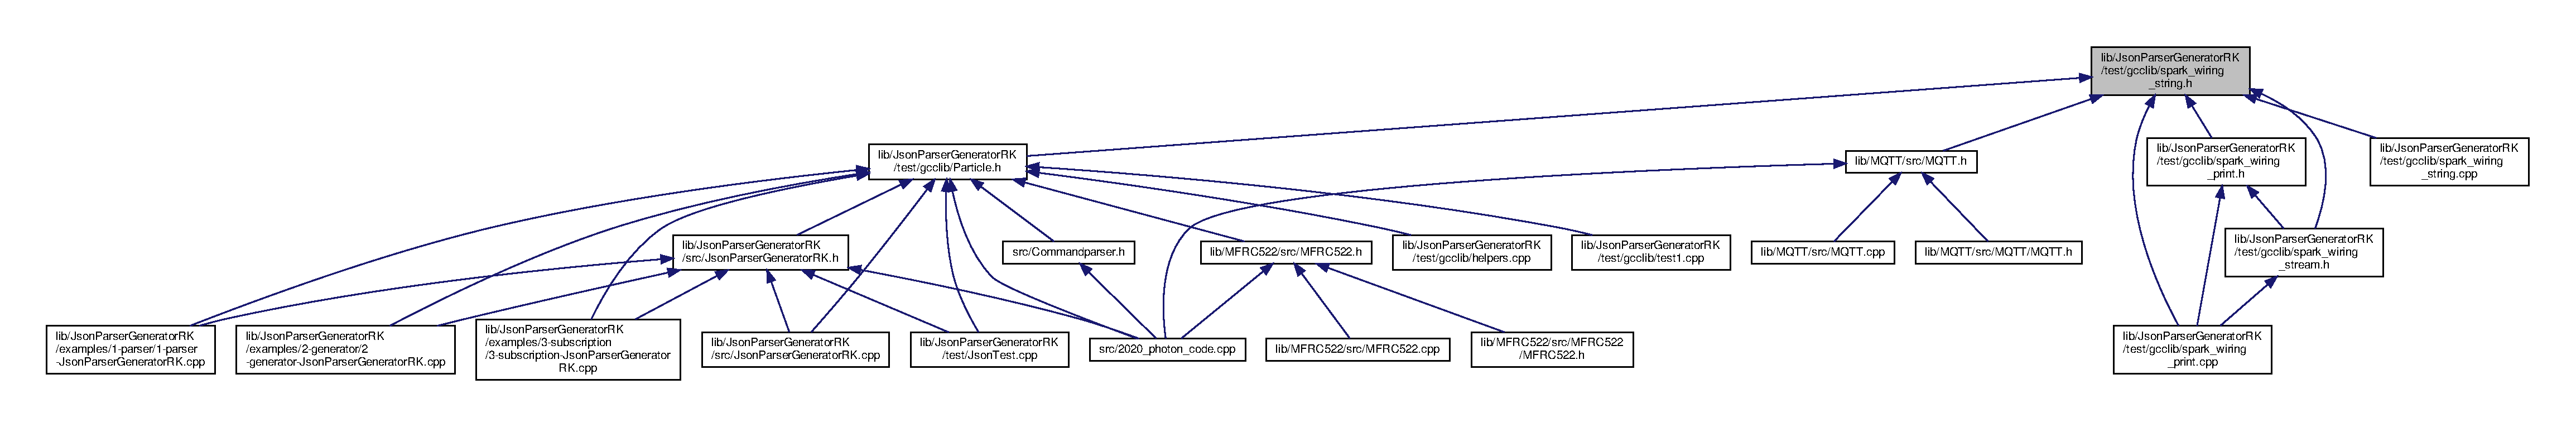
\includegraphics[width=350pt]{test_2gcclib_2spark__wiring__string_8h__dep__incl}
\end{center}
\end{figure}

\section{lib/\+Json\+Parser\+Generator\+R\+K/examples/1-\/parser/1-\/parser-\/\+Json\+Parser\+Generator\+RK.cpp File Reference}
\label{1-parser-_json_parser_generator_r_k_8cpp}\index{lib/\+Json\+Parser\+Generator\+R\+K/examples/1-\/parser/1-\/parser-\/\+Json\+Parser\+Generator\+R\+K.\+cpp@{lib/\+Json\+Parser\+Generator\+R\+K/examples/1-\/parser/1-\/parser-\/\+Json\+Parser\+Generator\+R\+K.\+cpp}}
{\ttfamily \#include \char`\"{}Particle.\+h\char`\"{}}\newline
{\ttfamily \#include \char`\"{}Json\+Parser\+Generator\+R\+K.\+h\char`\"{}}\newline
Include dependency graph for 1-\/parser-\/\+Json\+Parser\+Generator\+RK.cpp\+:\nopagebreak
\begin{figure}[H]
\begin{center}
\leavevmode
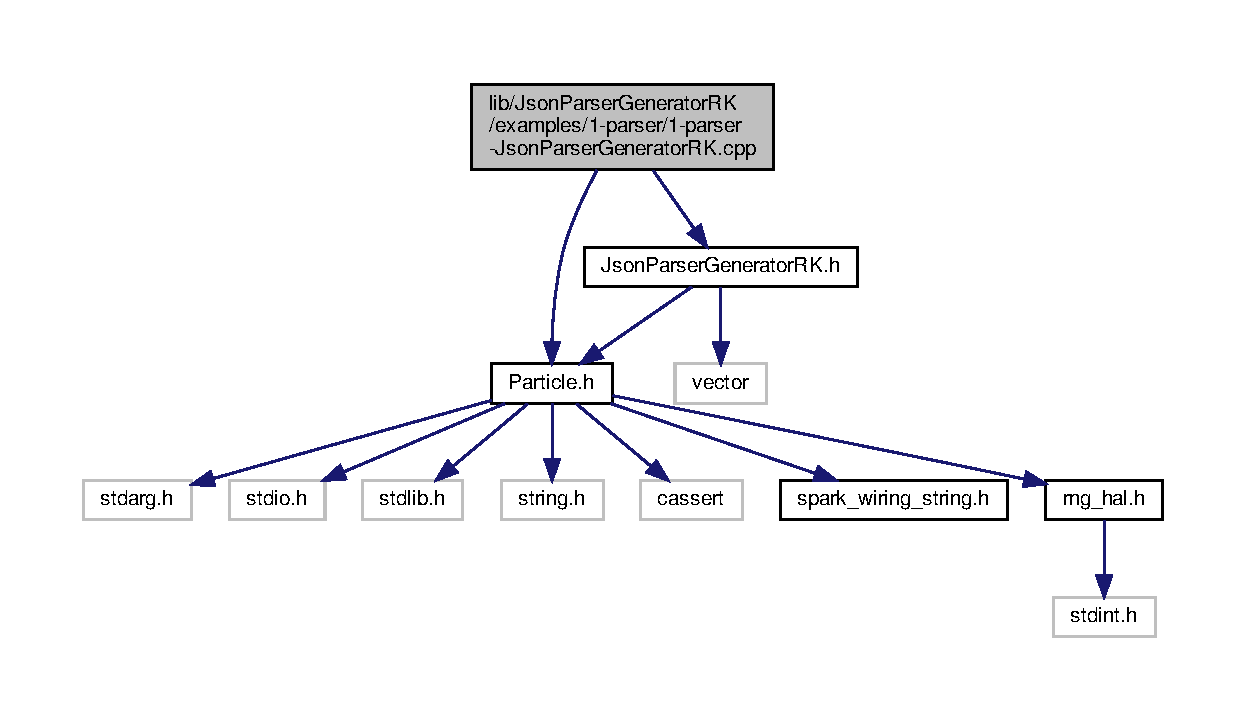
\includegraphics[width=350pt]{1-parser-_json_parser_generator_r_k_8cpp__incl}
\end{center}
\end{figure}
\subsection*{Functions}
\begin{DoxyCompactItemize}
\item 
void \textbf{ run\+Test} ()
\item 
void \textbf{ setup} ()
\begin{DoxyCompactList}\small\item\em Inital setup for pin assignments and serial links start. \end{DoxyCompactList}\item 
void \textbf{ loop} ()
\begin{DoxyCompactList}\small\item\em Main running function that executes all other functions; runs over 5times/second. \end{DoxyCompactList}\end{DoxyCompactItemize}
\subsection*{Variables}
\begin{DoxyCompactItemize}
\item 
const unsigned long \textbf{ T\+E\+S\+T\+\_\+\+R\+U\+N\+\_\+\+P\+E\+R\+I\+O\+D\+\_\+\+MS} = 10000
\item 
unsigned long \textbf{ last\+Run} = 0
\item 
const char $\ast$const \textbf{ test2} = \char`\"{}\{\textbackslash{}\char`\"{}t1\textbackslash{}\char`\"{}\+:\textbackslash{}\char`\"{}abc\textbackslash{}\char`\"{},\textbackslash{}\char`\"{}t2\textbackslash{}\char`\"{}\+:1234,\textbackslash{}\char`\"{}t3\textbackslash{}\char`\"{}\+:1234.\+5,\textbackslash{}\char`\"{}t4\textbackslash{}\char`\"{}\+:true,\textbackslash{}\char`\"{}t5\textbackslash{}\char`\"{}\+:false,\textbackslash{}\char`\"{}t6\textbackslash{}\char`\"{}\+:null, \textbackslash{}\char`\"{}t7\textbackslash{}\char`\"{} \+: \textbackslash{}\char`\"{}\textbackslash{}\textbackslash{}\textbackslash{}\char`\"{}quoted\textbackslash{}\textbackslash{}\textbackslash{}\char`\"{}\textbackslash{}\char`\"{} \} \char`\"{}
\item 
\textbf{ Json\+Parser\+Static}$<$ 256, 20 $>$ \textbf{ parser1}
\end{DoxyCompactItemize}


\subsection{Function Documentation}
\mbox{\label{1-parser-_json_parser_generator_r_k_8cpp_afe461d27b9c48d5921c00d521181f12f}} 
\index{1-\/parser-\/\+Json\+Parser\+Generator\+R\+K.\+cpp@{1-\/parser-\/\+Json\+Parser\+Generator\+R\+K.\+cpp}!loop@{loop}}
\index{loop@{loop}!1-\/parser-\/\+Json\+Parser\+Generator\+R\+K.\+cpp@{1-\/parser-\/\+Json\+Parser\+Generator\+R\+K.\+cpp}}
\subsubsection{loop()}
{\footnotesize\ttfamily void loop (\begin{DoxyParamCaption}{ }\end{DoxyParamCaption})}



Main running function that executes all other functions; runs over 5times/second. 



Definition at line 19 of file 1-\/parser-\/\+Json\+Parser\+Generator\+R\+K.\+cpp.



References run\+Test().


\begin{DoxyCode}
19             \{
20     \textcolor{keywordflow}{if} (millis() - lastRun >= TEST_RUN_PERIOD_MS) \{
21         lastRun = millis();
22         runTest();
23     \}
24 \}
\end{DoxyCode}
\mbox{\label{1-parser-_json_parser_generator_r_k_8cpp_a822f652c6fc2f163c182a6e5fe922c23}} 
\index{1-\/parser-\/\+Json\+Parser\+Generator\+R\+K.\+cpp@{1-\/parser-\/\+Json\+Parser\+Generator\+R\+K.\+cpp}!run\+Test@{run\+Test}}
\index{run\+Test@{run\+Test}!1-\/parser-\/\+Json\+Parser\+Generator\+R\+K.\+cpp@{1-\/parser-\/\+Json\+Parser\+Generator\+R\+K.\+cpp}}
\subsubsection{run\+Test()}
{\footnotesize\ttfamily void run\+Test (\begin{DoxyParamCaption}{ }\end{DoxyParamCaption})}



Definition at line 26 of file 1-\/parser-\/\+Json\+Parser\+Generator\+R\+K.\+cpp.



References Json\+Buffer\+::add\+String(), Json\+Buffer\+::clear(), Json\+Parser\+::get\+Outer\+Key\+Value\+By\+Index(), Json\+Parser\+::get\+Outer\+Value\+By\+Key(), String\+::operator!=(), Json\+Parser\+::parse(), parser1, and test2.


\begin{DoxyCode}
26                \{
27     \textcolor{comment}{// Clear the parser state, add the string test2, and parse it}
28     parser1.clear();
29     parser1.addString(test2);
30     \textcolor{keywordflow}{if} (!parser1.parse()) \{
31         Serial.println(\textcolor{stringliteral}{"parsing failed test2"});
32         \textcolor{keywordflow}{return};
33     \}
34 
35     String strValue;
36     \textcolor{keywordflow}{if} (!parser1.getOuterValueByKey(\textcolor{stringliteral}{"t1"}, strValue)) \{
37         Serial.println(\textcolor{stringliteral}{"failed to get test2 t1"});
38         \textcolor{keywordflow}{return};
39     \}
40     \textcolor{keywordflow}{if} (strValue != \textcolor{stringliteral}{"abc"}) \{
41         Serial.printlnf(\textcolor{stringliteral}{"wrong value test2 t1 was %s"}, strValue.c_str());
42         \textcolor{keywordflow}{return};
43     \}
44 
45     String keyName;
46     \textcolor{keywordflow}{if} (!parser1.getOuterKeyValueByIndex(0, keyName, strValue)) \{
47         Serial.println(\textcolor{stringliteral}{"failed to get test2 t1 by index"});
48         \textcolor{keywordflow}{return};
49     \}
50     \textcolor{keywordflow}{if} (keyName != \textcolor{stringliteral}{"t1"}) \{
51         Serial.printlnf(\textcolor{stringliteral}{"wrong key name test2 t1 was %s by index"}, keyName.c_str());
52         \textcolor{keywordflow}{return};
53     \}
54     \textcolor{keywordflow}{if} (strValue != \textcolor{stringliteral}{"abc"}) \{
55         Serial.printlnf(\textcolor{stringliteral}{"wrong value test2 t1 was %s by index"}, strValue.c_str());
56         \textcolor{keywordflow}{return};
57     \}
58 
59     \textcolor{keywordtype}{int} intValue;
60     \textcolor{keywordflow}{if} (!parser1.getOuterValueByKey(\textcolor{stringliteral}{"t2"}, intValue)) \{
61         Serial.println(\textcolor{stringliteral}{"failed to get test2 t2"});
62         \textcolor{keywordflow}{return};
63     \}
64     \textcolor{keywordflow}{if} (intValue != 1234) \{
65         Serial.printlnf(\textcolor{stringliteral}{"wrong value test2 t2 was %d"}, intValue);
66         \textcolor{keywordflow}{return};
67     \}
68     intValue = -1;
69 
70     \textcolor{keywordflow}{if} (!parser1.getOuterKeyValueByIndex(1, keyName, intValue)) \{
71         Serial.println(\textcolor{stringliteral}{"failed to get test2 t2 by index"});
72         \textcolor{keywordflow}{return};
73     \}
74     \textcolor{keywordflow}{if} (keyName != \textcolor{stringliteral}{"t2"}) \{
75         Serial.printlnf(\textcolor{stringliteral}{"wrong key name test2 t2 was %s by index"}, keyName.c_str());
76         \textcolor{keywordflow}{return};
77     \}
78     \textcolor{keywordflow}{if} (intValue != 1234) \{
79         Serial.printlnf(\textcolor{stringliteral}{"wrong value test2 t2 was %d by index"}, intValue);
80         \textcolor{keywordflow}{return};
81     \}
82 
83 
84     \textcolor{keywordtype}{float} floatValue;
85     \textcolor{keywordflow}{if} (!parser1.getOuterValueByKey(\textcolor{stringliteral}{"t3"}, floatValue)) \{
86         Serial.println(\textcolor{stringliteral}{"failed to get test2 t3"});
87         \textcolor{keywordflow}{return};
88     \}
89     \textcolor{keywordflow}{if} (floatValue != 1234.5) \{
90         Serial.printlnf(\textcolor{stringliteral}{"wrong value test2 t3 was %f"}, floatValue);
91         \textcolor{keywordflow}{return};
92     \}
93 
94     \textcolor{keywordtype}{bool} boolValue;
95     \textcolor{keywordflow}{if} (!parser1.getOuterValueByKey(\textcolor{stringliteral}{"t4"}, boolValue)) \{
96         Serial.println(\textcolor{stringliteral}{"failed to get test2 t4"});
97         \textcolor{keywordflow}{return};
98     \}
99     \textcolor{keywordflow}{if} (boolValue != \textcolor{keyword}{true}) \{
100         Serial.printlnf(\textcolor{stringliteral}{"wrong value test2 t4 was %d"}, boolValue);
101         \textcolor{keywordflow}{return};
102     \}
103 
104     \textcolor{keywordflow}{if} (!parser1.getOuterValueByKey(\textcolor{stringliteral}{"t5"}, boolValue)) \{
105         Serial.println(\textcolor{stringliteral}{"failed to get test2 t5"});
106         \textcolor{keywordflow}{return};
107     \}
108     \textcolor{keywordflow}{if} (boolValue != \textcolor{keyword}{false}) \{
109         Serial.printlnf(\textcolor{stringliteral}{"wrong value test2 t5 was %d"}, boolValue);
110         \textcolor{keywordflow}{return};
111     \}
112 
113 
114     \textcolor{keywordflow}{if} (!parser1.getOuterValueByKey(\textcolor{stringliteral}{"t7"}, strValue)) \{
115         Serial.println(\textcolor{stringliteral}{"failed to get test2 t7"});
116         \textcolor{keywordflow}{return};
117     \}
118     \textcolor{keywordflow}{if} (strValue != \textcolor{stringliteral}{"\(\backslash\)"quoted\(\backslash\)""}) \{
119         Serial.printlnf(\textcolor{stringliteral}{"wrong value test2 75 was %s"}, strValue.c_str());
120         \textcolor{keywordflow}{return};
121     \}
122 
123     Serial.println(\textcolor{stringliteral}{"test passed!"});
124 \}
\end{DoxyCode}
\mbox{\label{1-parser-_json_parser_generator_r_k_8cpp_a4fc01d736fe50cf5b977f755b675f11d}} 
\index{1-\/parser-\/\+Json\+Parser\+Generator\+R\+K.\+cpp@{1-\/parser-\/\+Json\+Parser\+Generator\+R\+K.\+cpp}!setup@{setup}}
\index{setup@{setup}!1-\/parser-\/\+Json\+Parser\+Generator\+R\+K.\+cpp@{1-\/parser-\/\+Json\+Parser\+Generator\+R\+K.\+cpp}}
\subsubsection{setup()}
{\footnotesize\ttfamily void setup (\begin{DoxyParamCaption}{ }\end{DoxyParamCaption})}



Inital setup for pin assignments and serial links start. 



Definition at line 15 of file 1-\/parser-\/\+Json\+Parser\+Generator\+R\+K.\+cpp.


\begin{DoxyCode}
15              \{
16     Serial.begin(9600);
17 \}
\end{DoxyCode}


\subsection{Variable Documentation}
\mbox{\label{1-parser-_json_parser_generator_r_k_8cpp_a5082951a06f690a0623ea99ed4228392}} 
\index{1-\/parser-\/\+Json\+Parser\+Generator\+R\+K.\+cpp@{1-\/parser-\/\+Json\+Parser\+Generator\+R\+K.\+cpp}!last\+Run@{last\+Run}}
\index{last\+Run@{last\+Run}!1-\/parser-\/\+Json\+Parser\+Generator\+R\+K.\+cpp@{1-\/parser-\/\+Json\+Parser\+Generator\+R\+K.\+cpp}}
\subsubsection{last\+Run}
{\footnotesize\ttfamily unsigned long last\+Run = 0}



Definition at line 6 of file 1-\/parser-\/\+Json\+Parser\+Generator\+R\+K.\+cpp.

\mbox{\label{1-parser-_json_parser_generator_r_k_8cpp_aa77335196b9c1b8ba3d649f2f381a009}} 
\index{1-\/parser-\/\+Json\+Parser\+Generator\+R\+K.\+cpp@{1-\/parser-\/\+Json\+Parser\+Generator\+R\+K.\+cpp}!parser1@{parser1}}
\index{parser1@{parser1}!1-\/parser-\/\+Json\+Parser\+Generator\+R\+K.\+cpp@{1-\/parser-\/\+Json\+Parser\+Generator\+R\+K.\+cpp}}
\subsubsection{parser1}
{\footnotesize\ttfamily \textbf{ Json\+Parser\+Static}$<$256, 20$>$ parser1}



Definition at line 13 of file 1-\/parser-\/\+Json\+Parser\+Generator\+R\+K.\+cpp.



Referenced by run\+Test().

\mbox{\label{1-parser-_json_parser_generator_r_k_8cpp_a27c66a6ddd571e937494116d9918691b}} 
\index{1-\/parser-\/\+Json\+Parser\+Generator\+R\+K.\+cpp@{1-\/parser-\/\+Json\+Parser\+Generator\+R\+K.\+cpp}!test2@{test2}}
\index{test2@{test2}!1-\/parser-\/\+Json\+Parser\+Generator\+R\+K.\+cpp@{1-\/parser-\/\+Json\+Parser\+Generator\+R\+K.\+cpp}}
\subsubsection{test2}
{\footnotesize\ttfamily const char$\ast$ const test2 = \char`\"{}\{\textbackslash{}\char`\"{}t1\textbackslash{}\char`\"{}\+:\textbackslash{}\char`\"{}abc\textbackslash{}\char`\"{},\textbackslash{}\char`\"{}t2\textbackslash{}\char`\"{}\+:1234,\textbackslash{}\char`\"{}t3\textbackslash{}\char`\"{}\+:1234.\+5,\textbackslash{}\char`\"{}t4\textbackslash{}\char`\"{}\+:true,\textbackslash{}\char`\"{}t5\textbackslash{}\char`\"{}\+:false,\textbackslash{}\char`\"{}t6\textbackslash{}\char`\"{}\+:null, \textbackslash{}\char`\"{}t7\textbackslash{}\char`\"{} \+: \textbackslash{}\char`\"{}\textbackslash{}\textbackslash{}\textbackslash{}\char`\"{}quoted\textbackslash{}\textbackslash{}\textbackslash{}\char`\"{}\textbackslash{}\char`\"{} \} \char`\"{}}



Definition at line 10 of file 1-\/parser-\/\+Json\+Parser\+Generator\+R\+K.\+cpp.



Referenced by run\+Test().

\mbox{\label{1-parser-_json_parser_generator_r_k_8cpp_a0aa12824a9c1a44e8d9f2499e0ba2698}} 
\index{1-\/parser-\/\+Json\+Parser\+Generator\+R\+K.\+cpp@{1-\/parser-\/\+Json\+Parser\+Generator\+R\+K.\+cpp}!T\+E\+S\+T\+\_\+\+R\+U\+N\+\_\+\+P\+E\+R\+I\+O\+D\+\_\+\+MS@{T\+E\+S\+T\+\_\+\+R\+U\+N\+\_\+\+P\+E\+R\+I\+O\+D\+\_\+\+MS}}
\index{T\+E\+S\+T\+\_\+\+R\+U\+N\+\_\+\+P\+E\+R\+I\+O\+D\+\_\+\+MS@{T\+E\+S\+T\+\_\+\+R\+U\+N\+\_\+\+P\+E\+R\+I\+O\+D\+\_\+\+MS}!1-\/parser-\/\+Json\+Parser\+Generator\+R\+K.\+cpp@{1-\/parser-\/\+Json\+Parser\+Generator\+R\+K.\+cpp}}
\subsubsection{T\+E\+S\+T\+\_\+\+R\+U\+N\+\_\+\+P\+E\+R\+I\+O\+D\+\_\+\+MS}
{\footnotesize\ttfamily const unsigned long T\+E\+S\+T\+\_\+\+R\+U\+N\+\_\+\+P\+E\+R\+I\+O\+D\+\_\+\+MS = 10000}



Definition at line 5 of file 1-\/parser-\/\+Json\+Parser\+Generator\+R\+K.\+cpp.


\hypertarget{2-generator-_json_parser_generator_r_k_8cpp}{}\section{lib/\+Json\+Parser\+Generator\+R\+K/examples/2-\/generator/2-\/generator-\/\+Json\+Parser\+Generator\+RK.cpp File Reference}
\label{2-generator-_json_parser_generator_r_k_8cpp}\index{lib/\+Json\+Parser\+Generator\+R\+K/examples/2-\/generator/2-\/generator-\/\+Json\+Parser\+Generator\+R\+K.\+cpp@{lib/\+Json\+Parser\+Generator\+R\+K/examples/2-\/generator/2-\/generator-\/\+Json\+Parser\+Generator\+R\+K.\+cpp}}
{\ttfamily \#include \char`\"{}Particle.\+h\char`\"{}}\newline
{\ttfamily \#include \char`\"{}Json\+Parser\+Generator\+R\+K.\+h\char`\"{}}\newline
Include dependency graph for 2-\/generator-\/\+Json\+Parser\+Generator\+RK.cpp\+:
\nopagebreak
\begin{figure}[H]
\begin{center}
\leavevmode
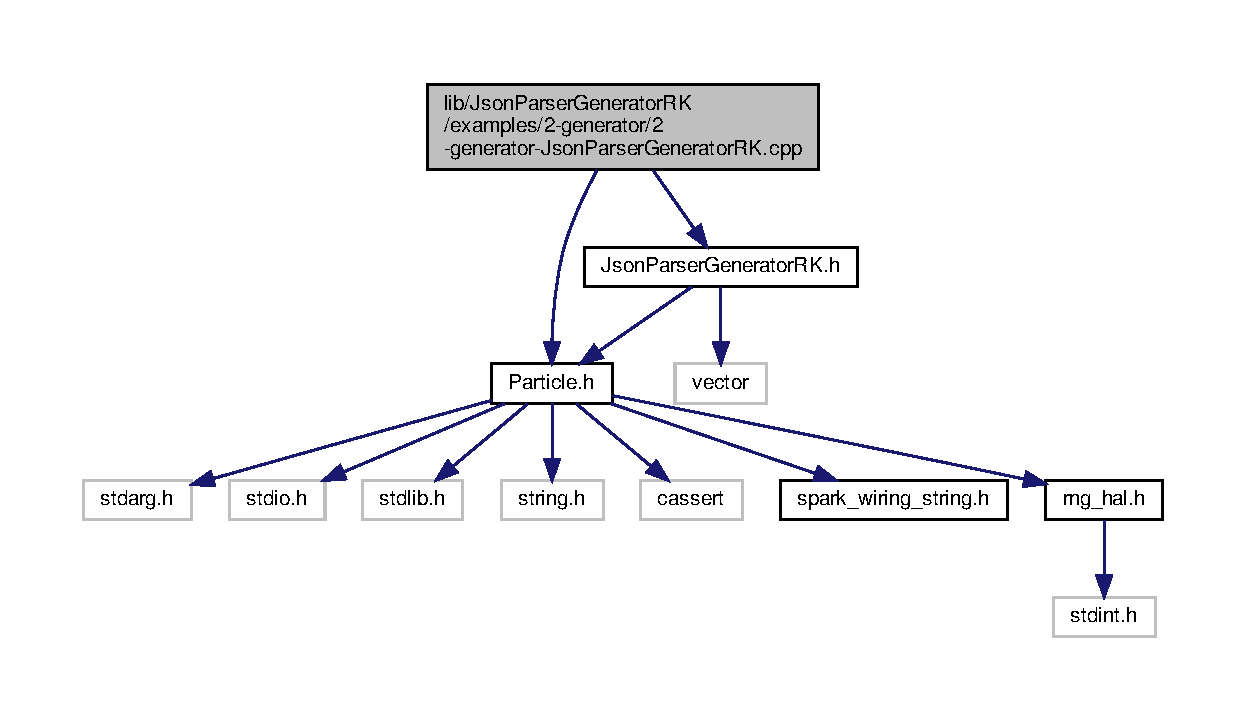
\includegraphics[width=287pt]{2-generator-_json_parser_generator_r_k_8cpp__incl}
\end{center}
\end{figure}
\subsection*{Functions}
\begin{DoxyCompactItemize}
\item 
void \hyperlink{2-generator-_json_parser_generator_r_k_8cpp_a822f652c6fc2f163c182a6e5fe922c23}{run\+Test} ()
\item 
void \hyperlink{2-generator-_json_parser_generator_r_k_8cpp_a4fc01d736fe50cf5b977f755b675f11d}{setup} ()
\item 
void \hyperlink{2-generator-_json_parser_generator_r_k_8cpp_afe461d27b9c48d5921c00d521181f12f}{loop} ()
\end{DoxyCompactItemize}
\subsection*{Variables}
\begin{DoxyCompactItemize}
\item 
const unsigned long \hyperlink{2-generator-_json_parser_generator_r_k_8cpp_a0aa12824a9c1a44e8d9f2499e0ba2698}{T\+E\+S\+T\+\_\+\+R\+U\+N\+\_\+\+P\+E\+R\+I\+O\+D\+\_\+\+MS} = 10000
\item 
unsigned long \hyperlink{2-generator-_json_parser_generator_r_k_8cpp_a5082951a06f690a0623ea99ed4228392}{last\+Run} = 0
\end{DoxyCompactItemize}


\subsection{Function Documentation}
\mbox{\Hypertarget{2-generator-_json_parser_generator_r_k_8cpp_afe461d27b9c48d5921c00d521181f12f}\label{2-generator-_json_parser_generator_r_k_8cpp_afe461d27b9c48d5921c00d521181f12f}} 
\index{2-\/generator-\/\+Json\+Parser\+Generator\+R\+K.\+cpp@{2-\/generator-\/\+Json\+Parser\+Generator\+R\+K.\+cpp}!loop@{loop}}
\index{loop@{loop}!2-\/generator-\/\+Json\+Parser\+Generator\+R\+K.\+cpp@{2-\/generator-\/\+Json\+Parser\+Generator\+R\+K.\+cpp}}
\subsubsection{\texorpdfstring{loop()}{loop()}}
{\footnotesize\ttfamily void loop (\begin{DoxyParamCaption}{ }\end{DoxyParamCaption})}



Definition at line 15 of file 2-\/generator-\/\+Json\+Parser\+Generator\+R\+K.\+cpp.



References run\+Test().

\mbox{\Hypertarget{2-generator-_json_parser_generator_r_k_8cpp_a822f652c6fc2f163c182a6e5fe922c23}\label{2-generator-_json_parser_generator_r_k_8cpp_a822f652c6fc2f163c182a6e5fe922c23}} 
\index{2-\/generator-\/\+Json\+Parser\+Generator\+R\+K.\+cpp@{2-\/generator-\/\+Json\+Parser\+Generator\+R\+K.\+cpp}!run\+Test@{run\+Test}}
\index{run\+Test@{run\+Test}!2-\/generator-\/\+Json\+Parser\+Generator\+R\+K.\+cpp@{2-\/generator-\/\+Json\+Parser\+Generator\+R\+K.\+cpp}}
\subsubsection{\texorpdfstring{run\+Test()}{runTest()}}
{\footnotesize\ttfamily void run\+Test (\begin{DoxyParamCaption}{ }\end{DoxyParamCaption})}



Definition at line 22 of file 2-\/generator-\/\+Json\+Parser\+Generator\+R\+K.\+cpp.



Referenced by loop().

\mbox{\Hypertarget{2-generator-_json_parser_generator_r_k_8cpp_a4fc01d736fe50cf5b977f755b675f11d}\label{2-generator-_json_parser_generator_r_k_8cpp_a4fc01d736fe50cf5b977f755b675f11d}} 
\index{2-\/generator-\/\+Json\+Parser\+Generator\+R\+K.\+cpp@{2-\/generator-\/\+Json\+Parser\+Generator\+R\+K.\+cpp}!setup@{setup}}
\index{setup@{setup}!2-\/generator-\/\+Json\+Parser\+Generator\+R\+K.\+cpp@{2-\/generator-\/\+Json\+Parser\+Generator\+R\+K.\+cpp}}
\subsubsection{\texorpdfstring{setup()}{setup()}}
{\footnotesize\ttfamily void setup (\begin{DoxyParamCaption}{ }\end{DoxyParamCaption})}



Definition at line 11 of file 2-\/generator-\/\+Json\+Parser\+Generator\+R\+K.\+cpp.



\subsection{Variable Documentation}
\mbox{\Hypertarget{2-generator-_json_parser_generator_r_k_8cpp_a5082951a06f690a0623ea99ed4228392}\label{2-generator-_json_parser_generator_r_k_8cpp_a5082951a06f690a0623ea99ed4228392}} 
\index{2-\/generator-\/\+Json\+Parser\+Generator\+R\+K.\+cpp@{2-\/generator-\/\+Json\+Parser\+Generator\+R\+K.\+cpp}!last\+Run@{last\+Run}}
\index{last\+Run@{last\+Run}!2-\/generator-\/\+Json\+Parser\+Generator\+R\+K.\+cpp@{2-\/generator-\/\+Json\+Parser\+Generator\+R\+K.\+cpp}}
\subsubsection{\texorpdfstring{last\+Run}{lastRun}}
{\footnotesize\ttfamily unsigned long last\+Run = 0}



Definition at line 6 of file 2-\/generator-\/\+Json\+Parser\+Generator\+R\+K.\+cpp.

\mbox{\Hypertarget{2-generator-_json_parser_generator_r_k_8cpp_a0aa12824a9c1a44e8d9f2499e0ba2698}\label{2-generator-_json_parser_generator_r_k_8cpp_a0aa12824a9c1a44e8d9f2499e0ba2698}} 
\index{2-\/generator-\/\+Json\+Parser\+Generator\+R\+K.\+cpp@{2-\/generator-\/\+Json\+Parser\+Generator\+R\+K.\+cpp}!T\+E\+S\+T\+\_\+\+R\+U\+N\+\_\+\+P\+E\+R\+I\+O\+D\+\_\+\+MS@{T\+E\+S\+T\+\_\+\+R\+U\+N\+\_\+\+P\+E\+R\+I\+O\+D\+\_\+\+MS}}
\index{T\+E\+S\+T\+\_\+\+R\+U\+N\+\_\+\+P\+E\+R\+I\+O\+D\+\_\+\+MS@{T\+E\+S\+T\+\_\+\+R\+U\+N\+\_\+\+P\+E\+R\+I\+O\+D\+\_\+\+MS}!2-\/generator-\/\+Json\+Parser\+Generator\+R\+K.\+cpp@{2-\/generator-\/\+Json\+Parser\+Generator\+R\+K.\+cpp}}
\subsubsection{\texorpdfstring{T\+E\+S\+T\+\_\+\+R\+U\+N\+\_\+\+P\+E\+R\+I\+O\+D\+\_\+\+MS}{TEST\_RUN\_PERIOD\_MS}}
{\footnotesize\ttfamily const unsigned long T\+E\+S\+T\+\_\+\+R\+U\+N\+\_\+\+P\+E\+R\+I\+O\+D\+\_\+\+MS = 10000}



Definition at line 5 of file 2-\/generator-\/\+Json\+Parser\+Generator\+R\+K.\+cpp.


\hypertarget{3-subscription-_json_parser_generator_r_k_8cpp}{}\section{lib/\+Json\+Parser\+Generator\+R\+K/examples/3-\/subscription/3-\/subscription-\/\+Json\+Parser\+Generator\+RK.cpp File Reference}
\label{3-subscription-_json_parser_generator_r_k_8cpp}\index{lib/\+Json\+Parser\+Generator\+R\+K/examples/3-\/subscription/3-\/subscription-\/\+Json\+Parser\+Generator\+R\+K.\+cpp@{lib/\+Json\+Parser\+Generator\+R\+K/examples/3-\/subscription/3-\/subscription-\/\+Json\+Parser\+Generator\+R\+K.\+cpp}}
{\ttfamily \#include \char`\"{}Particle.\+h\char`\"{}}\newline
{\ttfamily \#include \char`\"{}Json\+Parser\+Generator\+R\+K.\+h\char`\"{}}\newline
Include dependency graph for 3-\/subscription-\/\+Json\+Parser\+Generator\+RK.cpp\+:
\nopagebreak
\begin{figure}[H]
\begin{center}
\leavevmode
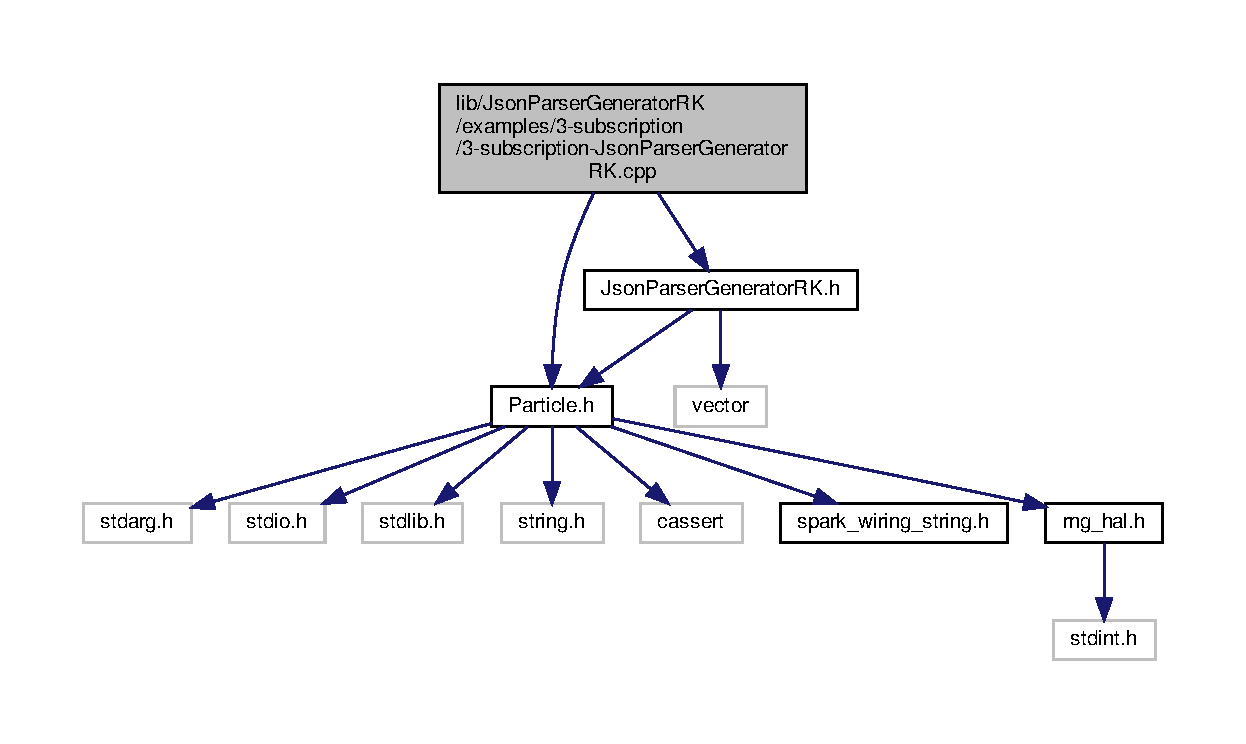
\includegraphics[width=350pt]{3-subscription-_json_parser_generator_r_k_8cpp__incl}
\end{center}
\end{figure}
\subsection*{Functions}
\begin{DoxyCompactItemize}
\item 
void \hyperlink{3-subscription-_json_parser_generator_r_k_8cpp_aa0bcca6652c4f60cb6e9bd893484650b}{subscription\+Handler} (const char $\ast$event, const char $\ast$data)
\item 
void \hyperlink{3-subscription-_json_parser_generator_r_k_8cpp_aa852eb9203676959147483523ec49997}{print\+Json} (\hyperlink{class_json_parser}{Json\+Parser} \&jp)
\item 
void \hyperlink{3-subscription-_json_parser_generator_r_k_8cpp_a4fc01d736fe50cf5b977f755b675f11d}{setup} ()
\item 
void \hyperlink{3-subscription-_json_parser_generator_r_k_8cpp_afe461d27b9c48d5921c00d521181f12f}{loop} ()
\item 
void \hyperlink{3-subscription-_json_parser_generator_r_k_8cpp_ae269cd10672ea800dd6fd6f14e48d0f8}{print\+Indent} (size\+\_\+t indent)
\item 
void \hyperlink{3-subscription-_json_parser_generator_r_k_8cpp_abe6d5621640c26d89a09be56928cd923}{print\+String} (const char $\ast$str)
\item 
void \hyperlink{3-subscription-_json_parser_generator_r_k_8cpp_a7a86f133587ae90abe048be568db828f}{print\+Json\+Inner} (\hyperlink{class_json_parser}{Json\+Parser} \&jp, const \hyperlink{struct_json_parser_generator_r_k_1_1jsmntok__t}{Json\+Parser\+Generator\+R\+K\+::jsmntok\+\_\+t} $\ast$container, size\+\_\+t indent)
\end{DoxyCompactItemize}
\subsection*{Variables}
\begin{DoxyCompactItemize}
\item 
\hyperlink{class_json_parser_static}{Json\+Parser\+Static}$<$ 2048, 100 $>$ \hyperlink{3-subscription-_json_parser_generator_r_k_8cpp_af1c065455ff8e2f533af5dd925c8469d}{json\+Parser}
\end{DoxyCompactItemize}


\subsection{Function Documentation}
\mbox{\Hypertarget{3-subscription-_json_parser_generator_r_k_8cpp_afe461d27b9c48d5921c00d521181f12f}\label{3-subscription-_json_parser_generator_r_k_8cpp_afe461d27b9c48d5921c00d521181f12f}} 
\index{3-\/subscription-\/\+Json\+Parser\+Generator\+R\+K.\+cpp@{3-\/subscription-\/\+Json\+Parser\+Generator\+R\+K.\+cpp}!loop@{loop}}
\index{loop@{loop}!3-\/subscription-\/\+Json\+Parser\+Generator\+R\+K.\+cpp@{3-\/subscription-\/\+Json\+Parser\+Generator\+R\+K.\+cpp}}
\subsubsection{\texorpdfstring{loop()}{loop()}}
{\footnotesize\ttfamily void loop (\begin{DoxyParamCaption}{ }\end{DoxyParamCaption})}



Definition at line 22 of file 3-\/subscription-\/\+Json\+Parser\+Generator\+R\+K.\+cpp.

\mbox{\Hypertarget{3-subscription-_json_parser_generator_r_k_8cpp_ae269cd10672ea800dd6fd6f14e48d0f8}\label{3-subscription-_json_parser_generator_r_k_8cpp_ae269cd10672ea800dd6fd6f14e48d0f8}} 
\index{3-\/subscription-\/\+Json\+Parser\+Generator\+R\+K.\+cpp@{3-\/subscription-\/\+Json\+Parser\+Generator\+R\+K.\+cpp}!print\+Indent@{print\+Indent}}
\index{print\+Indent@{print\+Indent}!3-\/subscription-\/\+Json\+Parser\+Generator\+R\+K.\+cpp@{3-\/subscription-\/\+Json\+Parser\+Generator\+R\+K.\+cpp}}
\subsubsection{\texorpdfstring{print\+Indent()}{printIndent()}}
{\footnotesize\ttfamily void print\+Indent (\begin{DoxyParamCaption}\item[{size\+\_\+t}]{indent }\end{DoxyParamCaption})}



Definition at line 47 of file 3-\/subscription-\/\+Json\+Parser\+Generator\+R\+K.\+cpp.

\mbox{\Hypertarget{3-subscription-_json_parser_generator_r_k_8cpp_aa852eb9203676959147483523ec49997}\label{3-subscription-_json_parser_generator_r_k_8cpp_aa852eb9203676959147483523ec49997}} 
\index{3-\/subscription-\/\+Json\+Parser\+Generator\+R\+K.\+cpp@{3-\/subscription-\/\+Json\+Parser\+Generator\+R\+K.\+cpp}!print\+Json@{print\+Json}}
\index{print\+Json@{print\+Json}!3-\/subscription-\/\+Json\+Parser\+Generator\+R\+K.\+cpp@{3-\/subscription-\/\+Json\+Parser\+Generator\+R\+K.\+cpp}}
\subsubsection{\texorpdfstring{print\+Json()}{printJson()}}
{\footnotesize\ttfamily void print\+Json (\begin{DoxyParamCaption}\item[{\hyperlink{class_json_parser}{Json\+Parser} \&}]{jp }\end{DoxyParamCaption})}



Definition at line 149 of file 3-\/subscription-\/\+Json\+Parser\+Generator\+R\+K.\+cpp.



References Json\+Parser\+::get\+Outer\+Token(), and print\+Json\+Inner().

\mbox{\Hypertarget{3-subscription-_json_parser_generator_r_k_8cpp_a7a86f133587ae90abe048be568db828f}\label{3-subscription-_json_parser_generator_r_k_8cpp_a7a86f133587ae90abe048be568db828f}} 
\index{3-\/subscription-\/\+Json\+Parser\+Generator\+R\+K.\+cpp@{3-\/subscription-\/\+Json\+Parser\+Generator\+R\+K.\+cpp}!print\+Json\+Inner@{print\+Json\+Inner}}
\index{print\+Json\+Inner@{print\+Json\+Inner}!3-\/subscription-\/\+Json\+Parser\+Generator\+R\+K.\+cpp@{3-\/subscription-\/\+Json\+Parser\+Generator\+R\+K.\+cpp}}
\subsubsection{\texorpdfstring{print\+Json\+Inner()}{printJsonInner()}}
{\footnotesize\ttfamily void print\+Json\+Inner (\begin{DoxyParamCaption}\item[{\hyperlink{class_json_parser}{Json\+Parser} \&}]{jp,  }\item[{const \hyperlink{struct_json_parser_generator_r_k_1_1jsmntok__t}{Json\+Parser\+Generator\+R\+K\+::jsmntok\+\_\+t} $\ast$}]{container,  }\item[{size\+\_\+t}]{indent }\end{DoxyParamCaption})}



Definition at line 75 of file 3-\/subscription-\/\+Json\+Parser\+Generator\+R\+K.\+cpp.



References Json\+Parser\+Generator\+R\+K\+::jsmntok\+\_\+t\+::end, Json\+Parser\+::get\+Key\+Value\+Token\+By\+Index(), Json\+Parser\+::get\+Token\+Value(), Json\+Parser\+::get\+Value\+Token\+By\+Index(), Json\+Parser\+Generator\+R\+K\+::\+J\+S\+M\+N\+\_\+\+A\+R\+R\+AY, Json\+Parser\+Generator\+R\+K\+::\+J\+S\+M\+N\+\_\+\+O\+B\+J\+E\+CT, Json\+Parser\+Generator\+R\+K\+::\+J\+S\+M\+N\+\_\+\+P\+R\+I\+M\+I\+T\+I\+VE, Json\+Parser\+Generator\+R\+K\+::\+J\+S\+M\+N\+\_\+\+S\+T\+R\+I\+NG, Json\+Parser\+Generator\+R\+K\+::\+J\+S\+M\+N\+\_\+\+U\+N\+D\+E\+F\+I\+N\+ED, print\+Indent(), print\+Json\+Inner(), print\+String(), Json\+Parser\+Generator\+R\+K\+::jsmntok\+\_\+t\+::start, and Json\+Parser\+Generator\+R\+K\+::jsmntok\+\_\+t\+::type.

\mbox{\Hypertarget{3-subscription-_json_parser_generator_r_k_8cpp_abe6d5621640c26d89a09be56928cd923}\label{3-subscription-_json_parser_generator_r_k_8cpp_abe6d5621640c26d89a09be56928cd923}} 
\index{3-\/subscription-\/\+Json\+Parser\+Generator\+R\+K.\+cpp@{3-\/subscription-\/\+Json\+Parser\+Generator\+R\+K.\+cpp}!print\+String@{print\+String}}
\index{print\+String@{print\+String}!3-\/subscription-\/\+Json\+Parser\+Generator\+R\+K.\+cpp@{3-\/subscription-\/\+Json\+Parser\+Generator\+R\+K.\+cpp}}
\subsubsection{\texorpdfstring{print\+String()}{printString()}}
{\footnotesize\ttfamily void print\+String (\begin{DoxyParamCaption}\item[{const char $\ast$}]{str }\end{DoxyParamCaption})}



Definition at line 53 of file 3-\/subscription-\/\+Json\+Parser\+Generator\+R\+K.\+cpp.

\mbox{\Hypertarget{3-subscription-_json_parser_generator_r_k_8cpp_a4fc01d736fe50cf5b977f755b675f11d}\label{3-subscription-_json_parser_generator_r_k_8cpp_a4fc01d736fe50cf5b977f755b675f11d}} 
\index{3-\/subscription-\/\+Json\+Parser\+Generator\+R\+K.\+cpp@{3-\/subscription-\/\+Json\+Parser\+Generator\+R\+K.\+cpp}!setup@{setup}}
\index{setup@{setup}!3-\/subscription-\/\+Json\+Parser\+Generator\+R\+K.\+cpp@{3-\/subscription-\/\+Json\+Parser\+Generator\+R\+K.\+cpp}}
\subsubsection{\texorpdfstring{setup()}{setup()}}
{\footnotesize\ttfamily void setup (\begin{DoxyParamCaption}{ }\end{DoxyParamCaption})}



Definition at line 17 of file 3-\/subscription-\/\+Json\+Parser\+Generator\+R\+K.\+cpp.

\mbox{\Hypertarget{3-subscription-_json_parser_generator_r_k_8cpp_aa0bcca6652c4f60cb6e9bd893484650b}\label{3-subscription-_json_parser_generator_r_k_8cpp_aa0bcca6652c4f60cb6e9bd893484650b}} 
\index{3-\/subscription-\/\+Json\+Parser\+Generator\+R\+K.\+cpp@{3-\/subscription-\/\+Json\+Parser\+Generator\+R\+K.\+cpp}!subscription\+Handler@{subscription\+Handler}}
\index{subscription\+Handler@{subscription\+Handler}!3-\/subscription-\/\+Json\+Parser\+Generator\+R\+K.\+cpp@{3-\/subscription-\/\+Json\+Parser\+Generator\+R\+K.\+cpp}}
\subsubsection{\texorpdfstring{subscription\+Handler()}{subscriptionHandler()}}
{\footnotesize\ttfamily void subscription\+Handler (\begin{DoxyParamCaption}\item[{const char $\ast$}]{event,  }\item[{const char $\ast$}]{data }\end{DoxyParamCaption})}



Definition at line 25 of file 3-\/subscription-\/\+Json\+Parser\+Generator\+R\+K.\+cpp.



References Json\+Buffer\+::add\+String(), Json\+Buffer\+::clear(), json\+Parser, Json\+Parser\+::parse(), and print\+Json().



\subsection{Variable Documentation}
\mbox{\Hypertarget{3-subscription-_json_parser_generator_r_k_8cpp_af1c065455ff8e2f533af5dd925c8469d}\label{3-subscription-_json_parser_generator_r_k_8cpp_af1c065455ff8e2f533af5dd925c8469d}} 
\index{3-\/subscription-\/\+Json\+Parser\+Generator\+R\+K.\+cpp@{3-\/subscription-\/\+Json\+Parser\+Generator\+R\+K.\+cpp}!json\+Parser@{json\+Parser}}
\index{json\+Parser@{json\+Parser}!3-\/subscription-\/\+Json\+Parser\+Generator\+R\+K.\+cpp@{3-\/subscription-\/\+Json\+Parser\+Generator\+R\+K.\+cpp}}
\subsubsection{\texorpdfstring{json\+Parser}{jsonParser}}
{\footnotesize\ttfamily \hyperlink{class_json_parser_static}{Json\+Parser\+Static}$<$2048, 100$>$ json\+Parser}



Definition at line 9 of file 3-\/subscription-\/\+Json\+Parser\+Generator\+R\+K.\+cpp.



Referenced by subscription\+Handler().


\hypertarget{lib_2_json_parser_generator_r_k_2_r_e_a_d_m_e_8md}{}\section{lib/\+Json\+Parser\+Generator\+R\+K/\+R\+E\+A\+D\+ME.md File Reference}
\label{lib_2_json_parser_generator_r_k_2_r_e_a_d_m_e_8md}\index{lib/\+Json\+Parser\+Generator\+R\+K/\+R\+E\+A\+D\+M\+E.\+md@{lib/\+Json\+Parser\+Generator\+R\+K/\+R\+E\+A\+D\+M\+E.\+md}}

\section{lib/\+M\+F\+R\+C522/\+R\+E\+A\+D\+ME.md File Reference}
\label{lib_2_m_f_r_c522_2_r_e_a_d_m_e_8md}\index{lib/\+M\+F\+R\+C522/\+R\+E\+A\+D\+M\+E.\+md@{lib/\+M\+F\+R\+C522/\+R\+E\+A\+D\+M\+E.\+md}}

\section{lib/\+M\+Q\+T\+T/\+R\+E\+A\+D\+ME.md File Reference}
\label{lib_2_m_q_t_t_2_r_e_a_d_m_e_8md}\index{lib/\+M\+Q\+T\+T/\+R\+E\+A\+D\+M\+E.\+md@{lib/\+M\+Q\+T\+T/\+R\+E\+A\+D\+M\+E.\+md}}

\hypertarget{_r_e_a_d_m_e_8md}{}\section{R\+E\+A\+D\+M\+E.\+md File Reference}
\label{_r_e_a_d_m_e_8md}\index{R\+E\+A\+D\+M\+E.\+md@{R\+E\+A\+D\+M\+E.\+md}}

\section{lib/\+Json\+Parser\+Generator\+R\+K/src/\+Json\+Parser\+Generator\+RK.cpp File Reference}
\label{_json_parser_generator_r_k_8cpp}\index{lib/\+Json\+Parser\+Generator\+R\+K/src/\+Json\+Parser\+Generator\+R\+K.\+cpp@{lib/\+Json\+Parser\+Generator\+R\+K/src/\+Json\+Parser\+Generator\+R\+K.\+cpp}}
{\ttfamily \#include \char`\"{}Particle.\+h\char`\"{}}\newline
{\ttfamily \#include \char`\"{}Json\+Parser\+Generator\+R\+K.\+h\char`\"{}}\newline
Include dependency graph for Json\+Parser\+Generator\+R\+K.\+cpp\+:\nopagebreak
\begin{figure}[H]
\begin{center}
\leavevmode
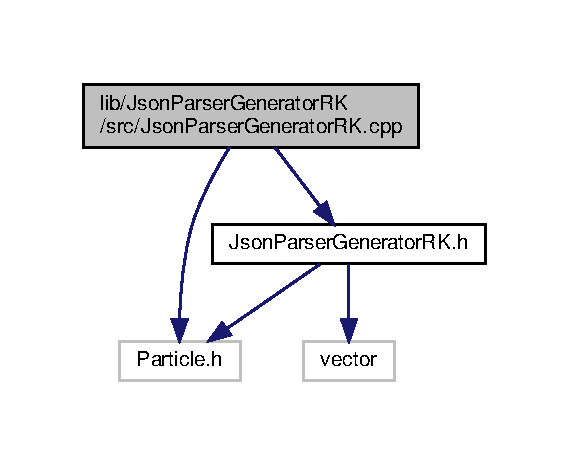
\includegraphics[width=350pt]{_json_parser_generator_r_k_8cpp__incl}
\end{center}
\end{figure}
\subsection*{Namespaces}
\begin{DoxyCompactItemize}
\item 
 \textbf{ Json\+Parser\+Generator\+RK}
\end{DoxyCompactItemize}
\subsection*{Functions}
\begin{DoxyCompactItemize}
\item 
static jsmntok\+\_\+t $\ast$ \textbf{ Json\+Parser\+Generator\+R\+K\+::jsmn\+\_\+alloc\+\_\+token} (jsmn\+\_\+parser $\ast$parser, jsmntok\+\_\+t $\ast$tokens, size\+\_\+t num\+\_\+tokens)
\item 
static void \textbf{ Json\+Parser\+Generator\+R\+K\+::jsmn\+\_\+fill\+\_\+token} (jsmntok\+\_\+t $\ast$token, jsmntype\+\_\+t type, int start, int end)
\item 
static int \textbf{ Json\+Parser\+Generator\+R\+K\+::jsmn\+\_\+parse\+\_\+primitive} (jsmn\+\_\+parser $\ast$parser, const char $\ast$js, size\+\_\+t len, jsmntok\+\_\+t $\ast$tokens, size\+\_\+t num\+\_\+tokens)
\item 
static int \textbf{ Json\+Parser\+Generator\+R\+K\+::jsmn\+\_\+parse\+\_\+string} (jsmn\+\_\+parser $\ast$parser, const char $\ast$js, size\+\_\+t len, jsmntok\+\_\+t $\ast$tokens, size\+\_\+t num\+\_\+tokens)
\item 
int \textbf{ Json\+Parser\+Generator\+R\+K\+::jsmn\+\_\+parse} (jsmn\+\_\+parser $\ast$parser, const char $\ast$js, size\+\_\+t len, jsmntok\+\_\+t $\ast$tokens, unsigned int num\+\_\+tokens)
\begin{DoxyCompactList}\small\item\em Run J\+S\+ON parser. \end{DoxyCompactList}\item 
void \textbf{ Json\+Parser\+Generator\+R\+K\+::jsmn\+\_\+init} (jsmn\+\_\+parser $\ast$parser)
\begin{DoxyCompactList}\small\item\em Create J\+S\+ON parser over an array of tokens. \end{DoxyCompactList}\end{DoxyCompactItemize}

\hypertarget{_json_parser_generator_r_k_8h}{}\section{lib/\+Json\+Parser\+Generator\+R\+K/src/\+Json\+Parser\+Generator\+RK.h File Reference}
\label{_json_parser_generator_r_k_8h}\index{lib/\+Json\+Parser\+Generator\+R\+K/src/\+Json\+Parser\+Generator\+R\+K.\+h@{lib/\+Json\+Parser\+Generator\+R\+K/src/\+Json\+Parser\+Generator\+R\+K.\+h}}
{\ttfamily \#include \char`\"{}Particle.\+h\char`\"{}}\newline
{\ttfamily \#include $<$vector$>$}\newline
Include dependency graph for Json\+Parser\+Generator\+R\+K.\+h\+:
\nopagebreak
\begin{figure}[H]
\begin{center}
\leavevmode
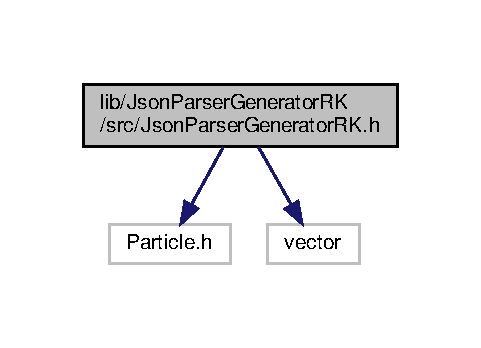
\includegraphics[width=350pt]{_json_parser_generator_r_k_8h__incl}
\end{center}
\end{figure}
This graph shows which files directly or indirectly include this file\+:
\nopagebreak
\begin{figure}[H]
\begin{center}
\leavevmode
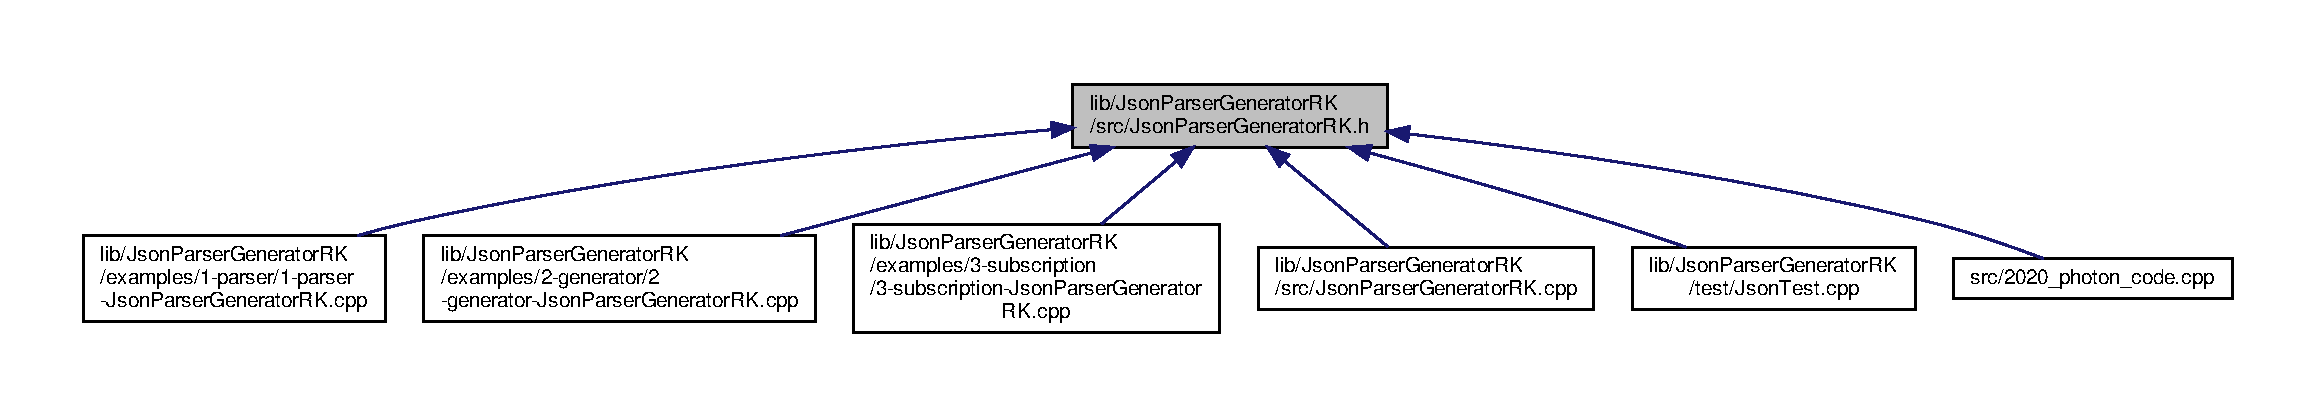
\includegraphics[width=350pt]{_json_parser_generator_r_k_8h__dep__incl}
\end{center}
\end{figure}
\subsection*{Classes}
\begin{DoxyCompactItemize}
\item 
struct \hyperlink{struct_json_parser_generator_r_k_1_1jsmntok__t}{Json\+Parser\+Generator\+R\+K\+::jsmntok\+\_\+t}
\begin{DoxyCompactList}\small\item\em J\+S\+ON token description. \end{DoxyCompactList}\item 
struct \hyperlink{struct_json_parser_generator_r_k_1_1jsmn__parser}{Json\+Parser\+Generator\+R\+K\+::jsmn\+\_\+parser}
\begin{DoxyCompactList}\small\item\em J\+S\+ON parser. \end{DoxyCompactList}\item 
class \hyperlink{class_json_parser_string}{Json\+Parser\+String}
\begin{DoxyCompactList}\small\item\em Class used internally for writing to strings. \end{DoxyCompactList}\item 
class \hyperlink{class_json_buffer}{Json\+Buffer}
\begin{DoxyCompactList}\small\item\em Base class for managing a static or dynamic buffer, used by both \hyperlink{class_json_parser}{Json\+Parser} and \hyperlink{class_json_writer}{Json\+Writer}. \end{DoxyCompactList}\item 
class \hyperlink{class_json_parser}{Json\+Parser}
\begin{DoxyCompactList}\small\item\em A\+PI to the \hyperlink{class_json_parser}{Json\+Parser}. \end{DoxyCompactList}\item 
class \hyperlink{class_json_parser_static}{Json\+Parser\+Static$<$ B\+U\+F\+F\+E\+R\+\_\+\+S\+I\+Z\+E, M\+A\+X\+\_\+\+T\+O\+K\+E\+N\+S $>$}
\begin{DoxyCompactList}\small\item\em Creates a \hyperlink{class_json_parser}{Json\+Parser} with a static buffer. \end{DoxyCompactList}\item 
class \hyperlink{class_json_reference}{Json\+Reference}
\begin{DoxyCompactList}\small\item\em This class provides a fluent-\/style A\+PI for easily traversing a tree of J\+S\+ON objects to find a value. \end{DoxyCompactList}\item 
struct \hyperlink{struct_json_writer_context}{Json\+Writer\+Context}
\begin{DoxyCompactList}\small\item\em Used internally by \hyperlink{class_json_writer}{Json\+Writer}. \end{DoxyCompactList}\item 
class \hyperlink{class_json_writer}{Json\+Writer}
\begin{DoxyCompactList}\small\item\em Class for building a J\+S\+ON string. \end{DoxyCompactList}\item 
class \hyperlink{class_json_writer_static}{Json\+Writer\+Static$<$ B\+U\+F\+F\+E\+R\+\_\+\+S\+I\+Z\+E $>$}
\begin{DoxyCompactList}\small\item\em Creates a \hyperlink{class_json_writer}{Json\+Writer} with a statically allocated buffer. \end{DoxyCompactList}\item 
class \hyperlink{class_json_writer_auto_object}{Json\+Writer\+Auto\+Object}
\begin{DoxyCompactList}\small\item\em Class for creating a J\+S\+ON object with \hyperlink{class_json_writer}{Json\+Writer}. \end{DoxyCompactList}\item 
class \hyperlink{class_json_writer_auto_array}{Json\+Writer\+Auto\+Array}
\begin{DoxyCompactList}\small\item\em Class for creating a J\+S\+ON array with \hyperlink{class_json_writer}{Json\+Writer}. \end{DoxyCompactList}\item 
class \hyperlink{class_json_modifier}{Json\+Modifier}
\begin{DoxyCompactList}\small\item\em Class for modifying a J\+S\+ON object in place, without needing to make a copy of it. \end{DoxyCompactList}\end{DoxyCompactItemize}
\subsection*{Namespaces}
\begin{DoxyCompactItemize}
\item 
 \hyperlink{namespace_json_parser_generator_r_k}{Json\+Parser\+Generator\+RK}
\end{DoxyCompactItemize}
\subsection*{Enumerations}
\begin{DoxyCompactItemize}
\item 
enum \hyperlink{namespace_json_parser_generator_r_k_a45d8af9d310679633d258ed9b2caeeb3}{Json\+Parser\+Generator\+R\+K\+::jsmntype\+\_\+t} \{ \newline
\hyperlink{namespace_json_parser_generator_r_k_a45d8af9d310679633d258ed9b2caeeb3af38a3f5a9af2aaf83f0fd6b38e6d80c5}{Json\+Parser\+Generator\+R\+K\+::\+J\+S\+M\+N\+\_\+\+U\+N\+D\+E\+F\+I\+N\+ED} = 0, 
\hyperlink{namespace_json_parser_generator_r_k_a45d8af9d310679633d258ed9b2caeeb3a821e92d4b14438ba747826d5b889fe48}{Json\+Parser\+Generator\+R\+K\+::\+J\+S\+M\+N\+\_\+\+O\+B\+J\+E\+CT} = 1, 
\hyperlink{namespace_json_parser_generator_r_k_a45d8af9d310679633d258ed9b2caeeb3a4f5a3b6dbf7ce0e6419264e11a7848c0}{Json\+Parser\+Generator\+R\+K\+::\+J\+S\+M\+N\+\_\+\+A\+R\+R\+AY} = 2, 
\hyperlink{namespace_json_parser_generator_r_k_a45d8af9d310679633d258ed9b2caeeb3a672e86ca38a72245272a29ecdbe74a1a}{Json\+Parser\+Generator\+R\+K\+::\+J\+S\+M\+N\+\_\+\+S\+T\+R\+I\+NG} = 3, 
\newline
\hyperlink{namespace_json_parser_generator_r_k_a45d8af9d310679633d258ed9b2caeeb3af36fefddaeac9a91bc69c938c8924568}{Json\+Parser\+Generator\+R\+K\+::\+J\+S\+M\+N\+\_\+\+P\+R\+I\+M\+I\+T\+I\+VE} = 4
 \}\begin{DoxyCompactList}\small\item\em J\+S\+ON type identifier (object, array, string, primitive) \end{DoxyCompactList}
\item 
enum \hyperlink{namespace_json_parser_generator_r_k_ab03a941ba316b9487a16636e6db43edf}{Json\+Parser\+Generator\+R\+K\+::jsmnerr} \{ \hyperlink{namespace_json_parser_generator_r_k_ab03a941ba316b9487a16636e6db43edfa629aaaf36d145f6b4968cb4a9ac9e2b1}{Json\+Parser\+Generator\+R\+K\+::\+J\+S\+M\+N\+\_\+\+E\+R\+R\+O\+R\+\_\+\+N\+O\+M\+EM} = -\/1, 
\hyperlink{namespace_json_parser_generator_r_k_ab03a941ba316b9487a16636e6db43edfa266cf322392ed180b57e6cd7ed6b77a6}{Json\+Parser\+Generator\+R\+K\+::\+J\+S\+M\+N\+\_\+\+E\+R\+R\+O\+R\+\_\+\+I\+N\+V\+AL} = -\/2, 
\hyperlink{namespace_json_parser_generator_r_k_ab03a941ba316b9487a16636e6db43edfafa021fb93449c243135e6158e1effa25}{Json\+Parser\+Generator\+R\+K\+::\+J\+S\+M\+N\+\_\+\+E\+R\+R\+O\+R\+\_\+\+P\+A\+RT} = -\/3
 \}\begin{DoxyCompactList}\small\item\em J\+S\+MN error codes. \end{DoxyCompactList}
\end{DoxyCompactItemize}
\subsection*{Functions}
\begin{DoxyCompactItemize}
\item 
void \hyperlink{namespace_json_parser_generator_r_k_adb1f5ae92d1df7b0b95f5caefbe0d55b}{Json\+Parser\+Generator\+R\+K\+::jsmn\+\_\+init} (jsmn\+\_\+parser $\ast$parser)
\begin{DoxyCompactList}\small\item\em Create J\+S\+ON parser over an array of tokens. \end{DoxyCompactList}\item 
int \hyperlink{namespace_json_parser_generator_r_k_acb71a39877526380a034824e99e59b75}{Json\+Parser\+Generator\+R\+K\+::jsmn\+\_\+parse} (jsmn\+\_\+parser $\ast$parser, const char $\ast$js, size\+\_\+t len, jsmntok\+\_\+t $\ast$tokens, unsigned int num\+\_\+tokens)
\begin{DoxyCompactList}\small\item\em Run J\+S\+ON parser. \end{DoxyCompactList}\end{DoxyCompactItemize}

\section{lib/\+Json\+Parser\+Generator\+R\+K/test/gcclib/helpers.cpp File Reference}
\label{helpers_8cpp}\index{lib/\+Json\+Parser\+Generator\+R\+K/test/gcclib/helpers.\+cpp@{lib/\+Json\+Parser\+Generator\+R\+K/test/gcclib/helpers.\+cpp}}
{\ttfamily \#include \char`\"{}Particle.\+h\char`\"{}}\newline
Include dependency graph for helpers.\+cpp\+:\nopagebreak
\begin{figure}[H]
\begin{center}
\leavevmode
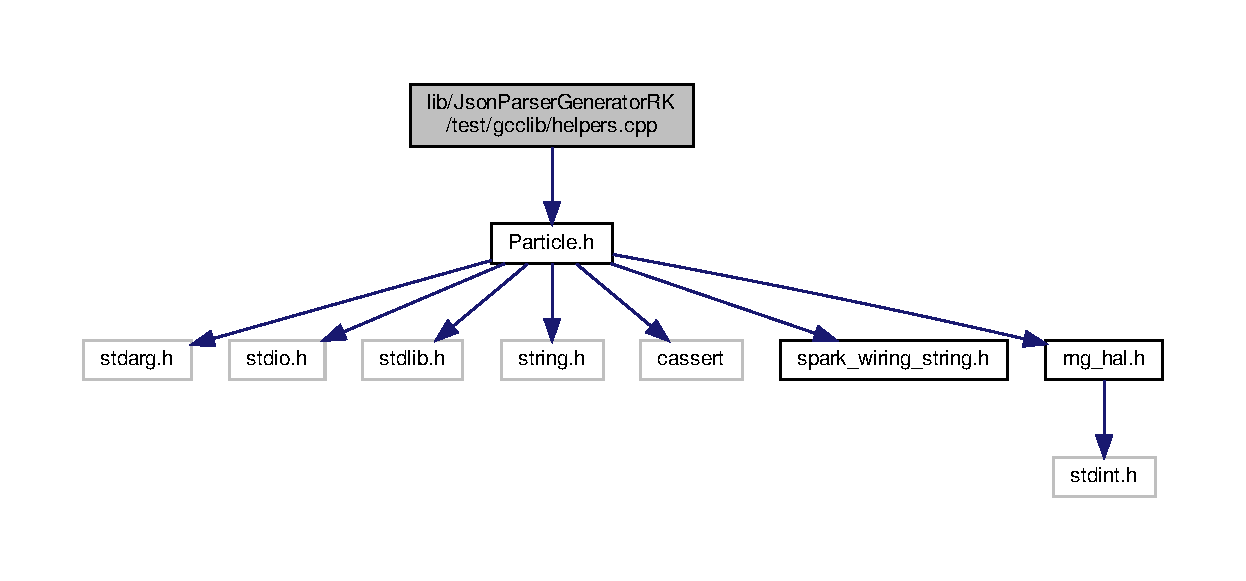
\includegraphics[width=350pt]{helpers_8cpp__incl}
\end{center}
\end{figure}
\subsection*{Functions}
\begin{DoxyCompactItemize}
\item 
char $\ast$ \textbf{ itoa} (int value, char $\ast$str, int base)
\item 
char $\ast$ \textbf{ utoa} (unsigned int value, char $\ast$str, int base)
\item 
char $\ast$ \textbf{ ltoa} (unsigned long value, char $\ast$str, int base)
\item 
char $\ast$ \textbf{ ultoa} (unsigned long value, char $\ast$str, int base)
\item 
uint32\+\_\+t \textbf{ H\+A\+L\+\_\+\+R\+N\+G\+\_\+\+Get\+Random\+Number} (void)
\end{DoxyCompactItemize}


\subsection{Function Documentation}
\mbox{\label{helpers_8cpp_abd7eeb850453afdae1e6ac00ecdae295}} 
\index{helpers.\+cpp@{helpers.\+cpp}!H\+A\+L\+\_\+\+R\+N\+G\+\_\+\+Get\+Random\+Number@{H\+A\+L\+\_\+\+R\+N\+G\+\_\+\+Get\+Random\+Number}}
\index{H\+A\+L\+\_\+\+R\+N\+G\+\_\+\+Get\+Random\+Number@{H\+A\+L\+\_\+\+R\+N\+G\+\_\+\+Get\+Random\+Number}!helpers.\+cpp@{helpers.\+cpp}}
\subsubsection{H\+A\+L\+\_\+\+R\+N\+G\+\_\+\+Get\+Random\+Number()}
{\footnotesize\ttfamily uint32\+\_\+t H\+A\+L\+\_\+\+R\+N\+G\+\_\+\+Get\+Random\+Number (\begin{DoxyParamCaption}\item[{void}]{ }\end{DoxyParamCaption})}



Definition at line 72 of file helpers.\+cpp.


\begin{DoxyCode}
72                                        \{
73     \textcolor{comment}{// This isn't right, there should be a cryptographically sound random number here,}
74     \textcolor{comment}{// but for testing this will be fine.}
75     \textcolor{keywordflow}{return} (uint32\_t) rand();
76 \}
\end{DoxyCode}
\mbox{\label{helpers_8cpp_ab42640268f26e065efd044cfe80591bd}} 
\index{helpers.\+cpp@{helpers.\+cpp}!itoa@{itoa}}
\index{itoa@{itoa}!helpers.\+cpp@{helpers.\+cpp}}
\subsubsection{itoa()}
{\footnotesize\ttfamily char$\ast$ itoa (\begin{DoxyParamCaption}\item[{int}]{value,  }\item[{char $\ast$}]{str,  }\item[{int}]{base }\end{DoxyParamCaption})}



Definition at line 4 of file helpers.\+cpp.



Referenced by String\+::concat(), and String\+::\+String().


\begin{DoxyCode}
4                                                \{
5 
6     \textcolor{keywordflow}{if} (base == 16) \{
7         sprintf(str, \textcolor{stringliteral}{"%x"}, value);
8     \}
9     \textcolor{keywordflow}{else}
10     \textcolor{keywordflow}{if} (base == 8) \{
11         sprintf(str, \textcolor{stringliteral}{"%o"}, value);
12     \}
13     \textcolor{keywordflow}{else} \{
14         sprintf(str, \textcolor{stringliteral}{"%d"}, value);
15     \}
16 
17     \textcolor{keywordflow}{return} str;
18 \}
\end{DoxyCode}
\mbox{\label{helpers_8cpp_a9343d51539e4cabc2457875cf5986aa7}} 
\index{helpers.\+cpp@{helpers.\+cpp}!ltoa@{ltoa}}
\index{ltoa@{ltoa}!helpers.\+cpp@{helpers.\+cpp}}
\subsubsection{ltoa()}
{\footnotesize\ttfamily char$\ast$ ltoa (\begin{DoxyParamCaption}\item[{unsigned long}]{value,  }\item[{char $\ast$}]{str,  }\item[{int}]{base }\end{DoxyParamCaption})}



Definition at line 38 of file helpers.\+cpp.


\begin{DoxyCode}
38                                                         \{
39 
40     \textcolor{keywordflow}{if} (base == 16) \{
41         sprintf(str, \textcolor{stringliteral}{"%lx"}, value);
42     \}
43     \textcolor{keywordflow}{else}
44     \textcolor{keywordflow}{if} (base == 8) \{
45         sprintf(str, \textcolor{stringliteral}{"%lo"}, value);
46     \}
47     \textcolor{keywordflow}{else} \{
48         sprintf(str, \textcolor{stringliteral}{"%ld"}, value);
49     \}
50 
51     \textcolor{keywordflow}{return} str;
52 \}
\end{DoxyCode}
\mbox{\label{helpers_8cpp_abcb262a9b96810d8483a665d6100f813}} 
\index{helpers.\+cpp@{helpers.\+cpp}!ultoa@{ultoa}}
\index{ultoa@{ultoa}!helpers.\+cpp@{helpers.\+cpp}}
\subsubsection{ultoa()}
{\footnotesize\ttfamily char$\ast$ ultoa (\begin{DoxyParamCaption}\item[{unsigned long}]{value,  }\item[{char $\ast$}]{str,  }\item[{int}]{base }\end{DoxyParamCaption})}



Definition at line 55 of file helpers.\+cpp.


\begin{DoxyCode}
55                                                          \{
56 
57     \textcolor{keywordflow}{if} (base == 16) \{
58         sprintf(str, \textcolor{stringliteral}{"%lx"}, value);
59     \}
60     \textcolor{keywordflow}{else}
61     \textcolor{keywordflow}{if} (base == 8) \{
62         sprintf(str, \textcolor{stringliteral}{"%lo"}, value);
63     \}
64     \textcolor{keywordflow}{else} \{
65         sprintf(str, \textcolor{stringliteral}{"%lu"}, value);
66     \}
67 
68     \textcolor{keywordflow}{return} str;
69 \}
\end{DoxyCode}
\mbox{\label{helpers_8cpp_a5a74d28d5863f08790d9457b84994276}} 
\index{helpers.\+cpp@{helpers.\+cpp}!utoa@{utoa}}
\index{utoa@{utoa}!helpers.\+cpp@{helpers.\+cpp}}
\subsubsection{utoa()}
{\footnotesize\ttfamily char$\ast$ utoa (\begin{DoxyParamCaption}\item[{unsigned int}]{value,  }\item[{char $\ast$}]{str,  }\item[{int}]{base }\end{DoxyParamCaption})}



Definition at line 21 of file helpers.\+cpp.


\begin{DoxyCode}
21                                                         \{
22 
23     \textcolor{keywordflow}{if} (base == 16) \{
24         sprintf(str, \textcolor{stringliteral}{"%x"}, value);
25     \}
26     \textcolor{keywordflow}{else}
27     \textcolor{keywordflow}{if} (base == 8) \{
28         sprintf(str, \textcolor{stringliteral}{"%o"}, value);
29     \}
30     \textcolor{keywordflow}{else} \{
31         sprintf(str, \textcolor{stringliteral}{"%u"}, value);
32     \}
33 
34     \textcolor{keywordflow}{return} str;
35 \}
\end{DoxyCode}

\hypertarget{_particle_8h}{}\section{lib/\+Json\+Parser\+Generator\+R\+K/test/gcclib/\+Particle.h File Reference}
\label{_particle_8h}\index{lib/\+Json\+Parser\+Generator\+R\+K/test/gcclib/\+Particle.\+h@{lib/\+Json\+Parser\+Generator\+R\+K/test/gcclib/\+Particle.\+h}}
{\ttfamily \#include $<$stdarg.\+h$>$}\newline
{\ttfamily \#include $<$stdio.\+h$>$}\newline
{\ttfamily \#include $<$stdlib.\+h$>$}\newline
{\ttfamily \#include $<$string.\+h$>$}\newline
{\ttfamily \#include $<$cassert$>$}\newline
{\ttfamily \#include \char`\"{}spark\+\_\+wiring\+\_\+string.\+h\char`\"{}}\newline
{\ttfamily \#include \char`\"{}rng\+\_\+hal.\+h\char`\"{}}\newline
Include dependency graph for Particle.\+h\+:
\nopagebreak
\begin{figure}[H]
\begin{center}
\leavevmode
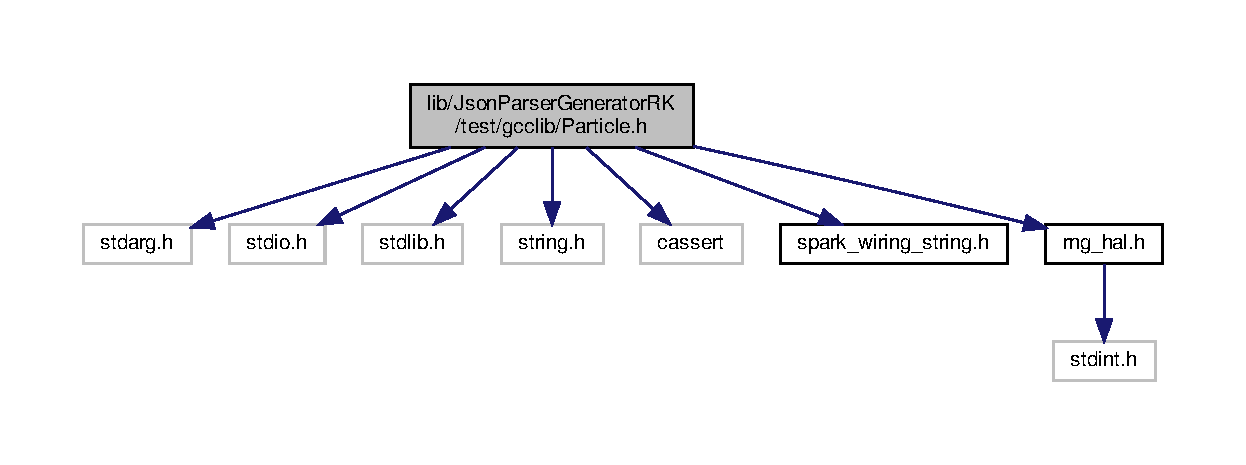
\includegraphics[width=350pt]{_particle_8h__incl}
\end{center}
\end{figure}
This graph shows which files directly or indirectly include this file\+:
\nopagebreak
\begin{figure}[H]
\begin{center}
\leavevmode
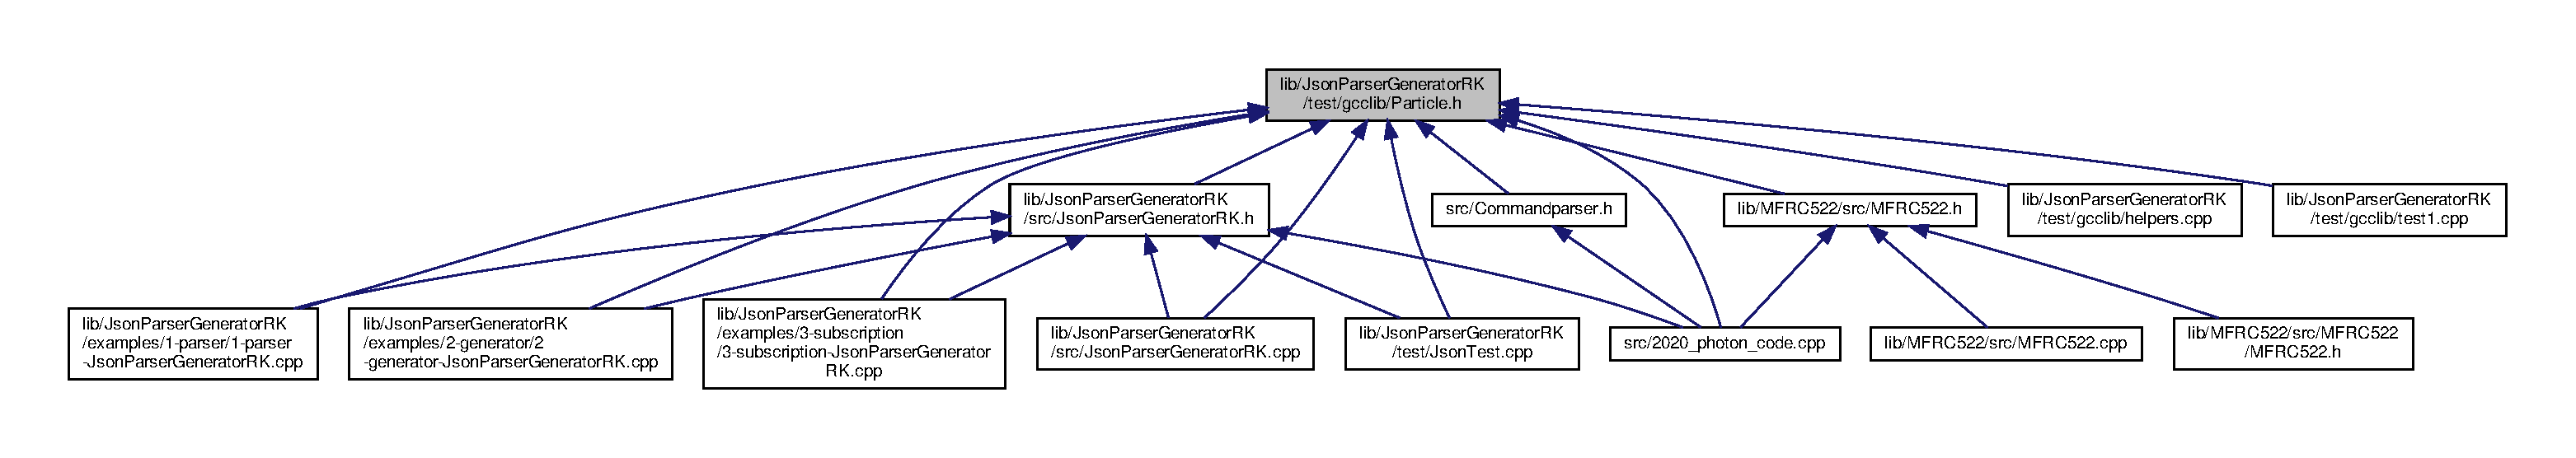
\includegraphics[width=350pt]{_particle_8h__dep__incl}
\end{center}
\end{figure}
\subsection*{Classes}
\begin{DoxyCompactItemize}
\item 
class \hyperlink{class_stream}{Stream}
\end{DoxyCompactItemize}

\hypertarget{rng__hal_8h}{}\section{lib/\+Json\+Parser\+Generator\+R\+K/test/gcclib/rng\+\_\+hal.h File Reference}
\label{rng__hal_8h}\index{lib/\+Json\+Parser\+Generator\+R\+K/test/gcclib/rng\+\_\+hal.\+h@{lib/\+Json\+Parser\+Generator\+R\+K/test/gcclib/rng\+\_\+hal.\+h}}


Copyright (c) 2015 Particle Industries, Inc. All rights reserved.  


{\ttfamily \#include $<$stdint.\+h$>$}\newline
Include dependency graph for rng\+\_\+hal.\+h\+:
\nopagebreak
\begin{figure}[H]
\begin{center}
\leavevmode
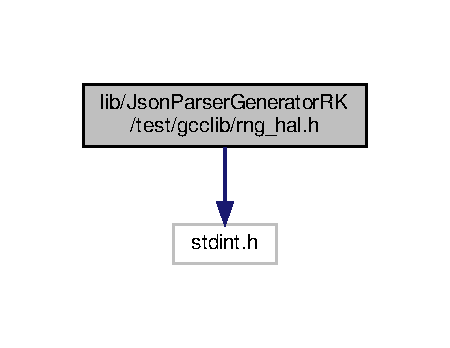
\includegraphics[width=216pt]{rng__hal_8h__incl}
\end{center}
\end{figure}
This graph shows which files directly or indirectly include this file\+:
\nopagebreak
\begin{figure}[H]
\begin{center}
\leavevmode
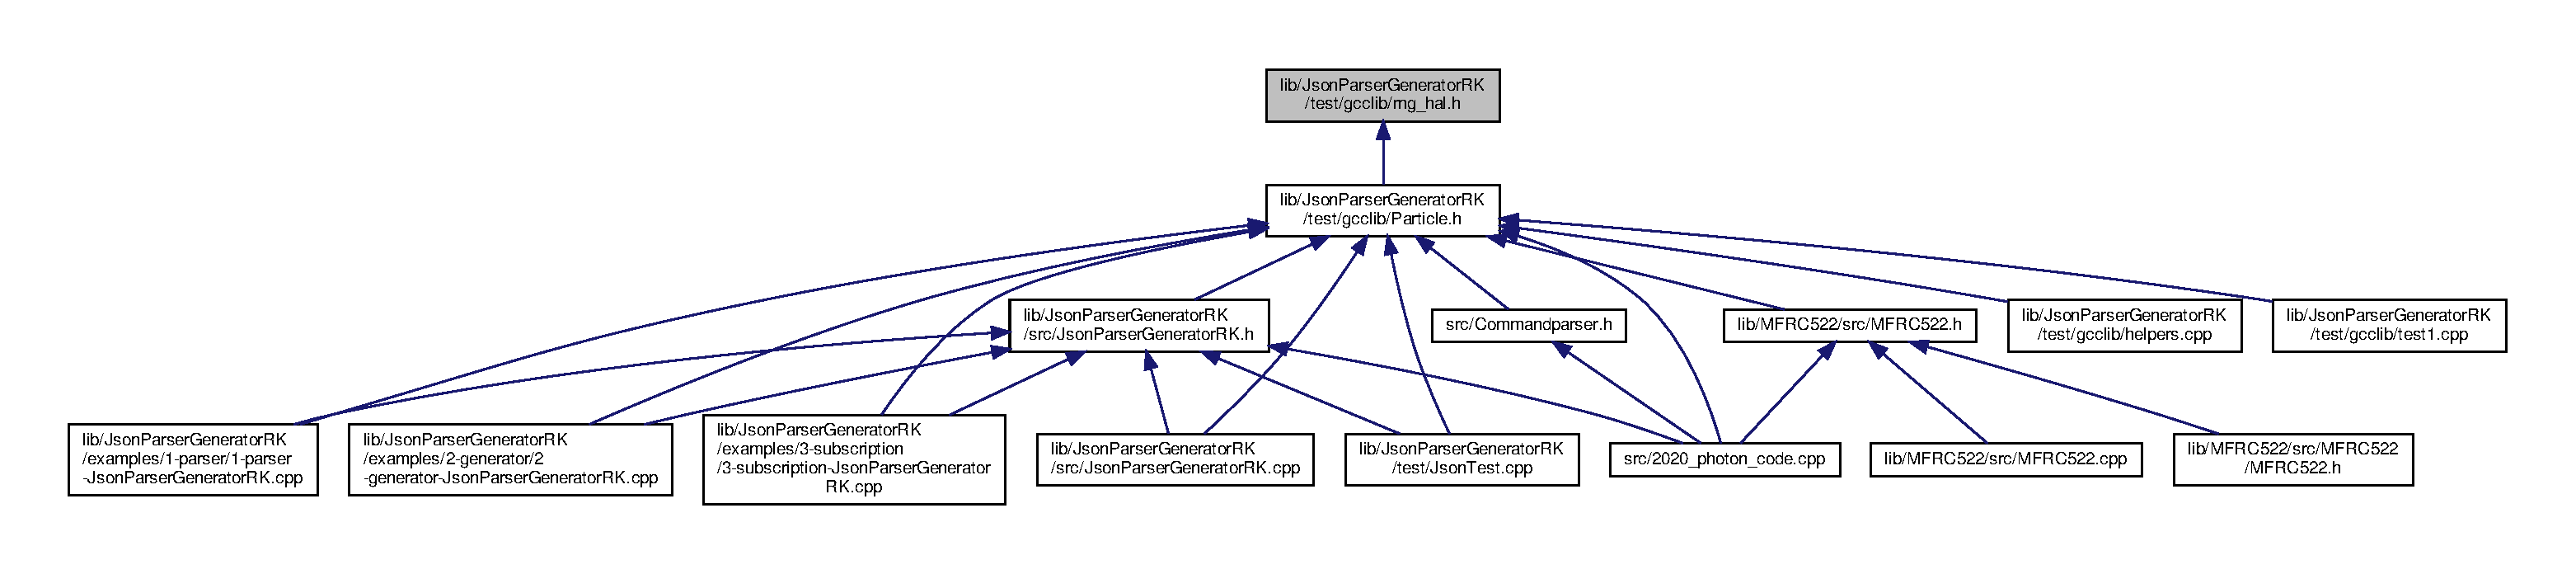
\includegraphics[width=350pt]{rng__hal_8h__dep__incl}
\end{center}
\end{figure}
\subsection*{Functions}
\begin{DoxyCompactItemize}
\item 
void \hyperlink{rng__hal_8h_a5789cde5621c72ba09128cc7f0d84531}{H\+A\+L\+\_\+\+R\+N\+G\+\_\+\+Configuration} (void)
\item 
uint32\+\_\+t \hyperlink{rng__hal_8h_abd7eeb850453afdae1e6ac00ecdae295}{H\+A\+L\+\_\+\+R\+N\+G\+\_\+\+Get\+Random\+Number} (void)
\end{DoxyCompactItemize}


\subsection{Detailed Description}
Copyright (c) 2015 Particle Industries, Inc. All rights reserved. 

\begin{DoxyAuthor}{Author}
Satish Nair 
\end{DoxyAuthor}
\begin{DoxyVersion}{Version}
V1.\+0.\+0 
\end{DoxyVersion}
\begin{DoxyDate}{Date}
13-\/\+Jan-\/2015 This library is free software; you can redistribute it and/or modify it under the terms of the G\+NU Lesser General Public License as published by the Free Software Foundation, either version 3 of the License, or (at your option) any later version.
\end{DoxyDate}
This library is distributed in the hope that it will be useful, but W\+I\+T\+H\+O\+UT A\+NY W\+A\+R\+R\+A\+N\+TY; without even the implied warranty of M\+E\+R\+C\+H\+A\+N\+T\+A\+B\+I\+L\+I\+TY or F\+I\+T\+N\+E\+SS F\+OR A P\+A\+R\+T\+I\+C\+U\+L\+AR P\+U\+R\+P\+O\+SE. See the G\+NU Lesser General Public License for more details.

You should have received a copy of the G\+NU Lesser General Public License along with this library; if not, see \href{http://www.gnu.org/licenses/}{\tt http\+://www.\+gnu.\+org/licenses/}. 

\subsection{Function Documentation}
\mbox{\Hypertarget{rng__hal_8h_a5789cde5621c72ba09128cc7f0d84531}\label{rng__hal_8h_a5789cde5621c72ba09128cc7f0d84531}} 
\index{rng\+\_\+hal.\+h@{rng\+\_\+hal.\+h}!H\+A\+L\+\_\+\+R\+N\+G\+\_\+\+Configuration@{H\+A\+L\+\_\+\+R\+N\+G\+\_\+\+Configuration}}
\index{H\+A\+L\+\_\+\+R\+N\+G\+\_\+\+Configuration@{H\+A\+L\+\_\+\+R\+N\+G\+\_\+\+Configuration}!rng\+\_\+hal.\+h@{rng\+\_\+hal.\+h}}
\subsubsection{\texorpdfstring{H\+A\+L\+\_\+\+R\+N\+G\+\_\+\+Configuration()}{HAL\_RNG\_Configuration()}}
{\footnotesize\ttfamily void H\+A\+L\+\_\+\+R\+N\+G\+\_\+\+Configuration (\begin{DoxyParamCaption}\item[{void}]{ }\end{DoxyParamCaption})}

\mbox{\Hypertarget{rng__hal_8h_abd7eeb850453afdae1e6ac00ecdae295}\label{rng__hal_8h_abd7eeb850453afdae1e6ac00ecdae295}} 
\index{rng\+\_\+hal.\+h@{rng\+\_\+hal.\+h}!H\+A\+L\+\_\+\+R\+N\+G\+\_\+\+Get\+Random\+Number@{H\+A\+L\+\_\+\+R\+N\+G\+\_\+\+Get\+Random\+Number}}
\index{H\+A\+L\+\_\+\+R\+N\+G\+\_\+\+Get\+Random\+Number@{H\+A\+L\+\_\+\+R\+N\+G\+\_\+\+Get\+Random\+Number}!rng\+\_\+hal.\+h@{rng\+\_\+hal.\+h}}
\subsubsection{\texorpdfstring{H\+A\+L\+\_\+\+R\+N\+G\+\_\+\+Get\+Random\+Number()}{HAL\_RNG\_GetRandomNumber()}}
{\footnotesize\ttfamily uint32\+\_\+t H\+A\+L\+\_\+\+R\+N\+G\+\_\+\+Get\+Random\+Number (\begin{DoxyParamCaption}\item[{void}]{ }\end{DoxyParamCaption})}



Definition at line 72 of file helpers.\+cpp.


\hypertarget{spark__wiring__print_8cpp}{}\section{lib/\+Json\+Parser\+Generator\+R\+K/test/gcclib/spark\+\_\+wiring\+\_\+print.cpp File Reference}
\label{spark__wiring__print_8cpp}\index{lib/\+Json\+Parser\+Generator\+R\+K/test/gcclib/spark\+\_\+wiring\+\_\+print.\+cpp@{lib/\+Json\+Parser\+Generator\+R\+K/test/gcclib/spark\+\_\+wiring\+\_\+print.\+cpp}}


Wrapper for wiring print.  


{\ttfamily \#include $<$math.\+h$>$}\newline
{\ttfamily \#include $<$stdarg.\+h$>$}\newline
{\ttfamily \#include $<$stdio.\+h$>$}\newline
{\ttfamily \#include \char`\"{}spark\+\_\+wiring\+\_\+print.\+h\char`\"{}}\newline
{\ttfamily \#include \char`\"{}spark\+\_\+wiring\+\_\+string.\+h\char`\"{}}\newline
{\ttfamily \#include \char`\"{}spark\+\_\+wiring\+\_\+stream.\+h\char`\"{}}\newline
Include dependency graph for spark\+\_\+wiring\+\_\+print.\+cpp\+:
\nopagebreak
\begin{figure}[H]
\begin{center}
\leavevmode
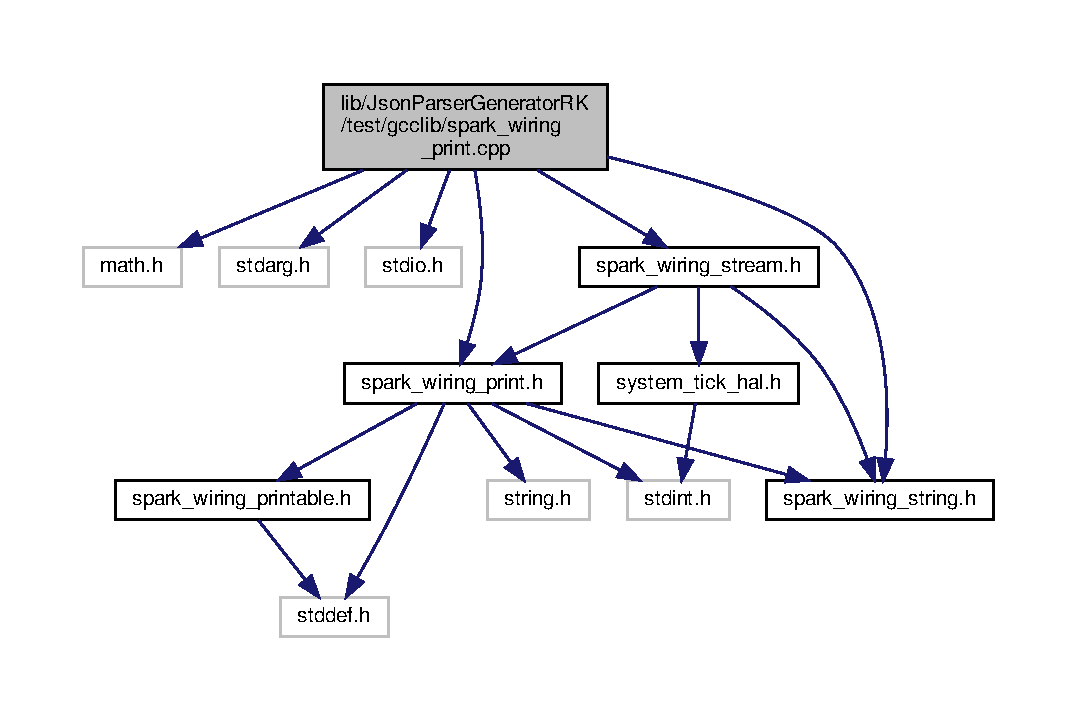
\includegraphics[width=350pt]{spark__wiring__print_8cpp__incl}
\end{center}
\end{figure}


\subsection{Detailed Description}
Wrapper for wiring print. 

\begin{DoxyAuthor}{Author}
Mohit Bhoite 
\end{DoxyAuthor}
\begin{DoxyVersion}{Version}
V1.\+0.\+0 
\end{DoxyVersion}
\begin{DoxyDate}{Date}
13-\/\+March-\/2013 Copyright (c) 2013-\/2015 Particle Industries, Inc. All rights reserved. Copyright (c) 2010 David A. Mellis. All right reserved.
\end{DoxyDate}
This library is free software; you can redistribute it and/or modify it under the terms of the G\+NU Lesser General Public License as published by the Free Software Foundation, either version 3 of the License, or (at your option) any later version.

This library is distributed in the hope that it will be useful, but W\+I\+T\+H\+O\+UT A\+NY W\+A\+R\+R\+A\+N\+TY; without even the implied warranty of M\+E\+R\+C\+H\+A\+N\+T\+A\+B\+I\+L\+I\+TY or F\+I\+T\+N\+E\+SS F\+OR A P\+A\+R\+T\+I\+C\+U\+L\+AR P\+U\+R\+P\+O\+SE. See the G\+NU Lesser General Public License for more details.

You should have received a copy of the G\+NU Lesser General Public License along with this library; if not, see \href{http://www.gnu.org/licenses/}{\tt http\+://www.\+gnu.\+org/licenses/}. 
\hypertarget{spark__wiring__stream_8h}{}\section{lib/\+Json\+Parser\+Generator\+R\+K/test/gcclib/spark\+\_\+wiring\+\_\+stream.h File Reference}
\label{spark__wiring__stream_8h}\index{lib/\+Json\+Parser\+Generator\+R\+K/test/gcclib/spark\+\_\+wiring\+\_\+stream.\+h@{lib/\+Json\+Parser\+Generator\+R\+K/test/gcclib/spark\+\_\+wiring\+\_\+stream.\+h}}


Header for spark\+\_\+wiring\+\_\+stream.\+c module.  


{\ttfamily \#include \char`\"{}spark\+\_\+wiring\+\_\+string.\+h\char`\"{}}\newline
{\ttfamily \#include \char`\"{}spark\+\_\+wiring\+\_\+print.\+h\char`\"{}}\newline
{\ttfamily \#include \char`\"{}system\+\_\+tick\+\_\+hal.\+h\char`\"{}}\newline
Include dependency graph for spark\+\_\+wiring\+\_\+stream.\+h\+:
\nopagebreak
\begin{figure}[H]
\begin{center}
\leavevmode
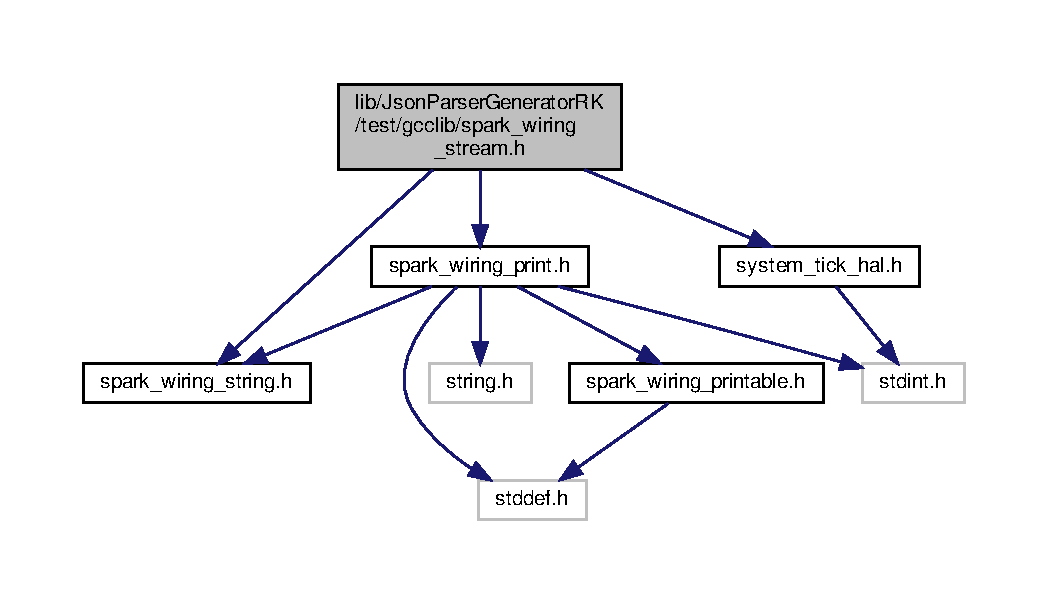
\includegraphics[width=350pt]{spark__wiring__stream_8h__incl}
\end{center}
\end{figure}
This graph shows which files directly or indirectly include this file\+:
\nopagebreak
\begin{figure}[H]
\begin{center}
\leavevmode
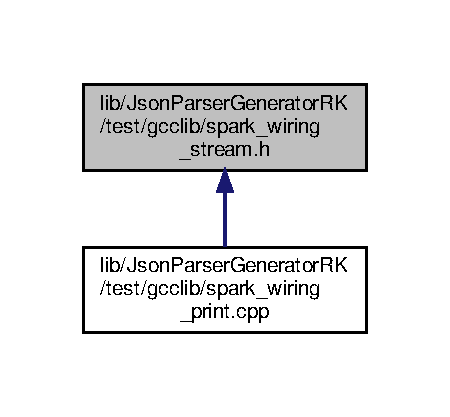
\includegraphics[width=216pt]{spark__wiring__stream_8h__dep__incl}
\end{center}
\end{figure}
\subsection*{Classes}
\begin{DoxyCompactItemize}
\item 
class \hyperlink{class_stream}{Stream}
\end{DoxyCompactItemize}


\subsection{Detailed Description}
Header for spark\+\_\+wiring\+\_\+stream.\+c module. 

\begin{DoxyAuthor}{Author}
Mohit Bhoite 
\end{DoxyAuthor}
\begin{DoxyVersion}{Version}
V1.\+0.\+0 
\end{DoxyVersion}
\begin{DoxyDate}{Date}
13-\/\+March-\/2013 Copyright (c) 2013-\/2015 Particle Industries, Inc. All rights reserved. Copyright (c) 2010 David A. Mellis. All right reserved.
\end{DoxyDate}
This library is free software; you can redistribute it and/or modify it under the terms of the G\+NU Lesser General Public License as published by the Free Software Foundation, either version 3 of the License, or (at your option) any later version.

This library is distributed in the hope that it will be useful, but W\+I\+T\+H\+O\+UT A\+NY W\+A\+R\+R\+A\+N\+TY; without even the implied warranty of M\+E\+R\+C\+H\+A\+N\+T\+A\+B\+I\+L\+I\+TY or F\+I\+T\+N\+E\+SS F\+OR A P\+A\+R\+T\+I\+C\+U\+L\+AR P\+U\+R\+P\+O\+SE. See the G\+NU Lesser General Public License for more details.

You should have received a copy of the G\+NU Lesser General Public License along with this library; if not, see \href{http://www.gnu.org/licenses/}{\tt http\+://www.\+gnu.\+org/licenses/}. 
\hypertarget{spark__wiring__string_8cpp}{}\section{lib/\+Json\+Parser\+Generator\+R\+K/test/gcclib/spark\+\_\+wiring\+\_\+string.cpp File Reference}
\label{spark__wiring__string_8cpp}\index{lib/\+Json\+Parser\+Generator\+R\+K/test/gcclib/spark\+\_\+wiring\+\_\+string.\+cpp@{lib/\+Json\+Parser\+Generator\+R\+K/test/gcclib/spark\+\_\+wiring\+\_\+string.\+cpp}}


Copyright (c) 2013-\/2015 Particle Industries, Inc. All rights reserved. ...mostly rewritten by Paul Stoffregen... Copyright (c) 2009-\/10 Hernando Barragan. All rights reserved. Copyright 2011, Paul Stoffregen, \href{mailto:paul@pjrc.com}{\tt paul@pjrc.\+com}.  


{\ttfamily \#include \char`\"{}spark\+\_\+wiring\+\_\+string.\+h\char`\"{}}\newline
{\ttfamily \#include $<$stdio.\+h$>$}\newline
{\ttfamily \#include $<$limits.\+h$>$}\newline
{\ttfamily \#include $<$ctype.\+h$>$}\newline
{\ttfamily \#include $<$stdlib.\+h$>$}\newline
{\ttfamily \#include \char`\"{}string\+\_\+convert.\+h\char`\"{}}\newline
Include dependency graph for spark\+\_\+wiring\+\_\+string.\+cpp\+:
\nopagebreak
\begin{figure}[H]
\begin{center}
\leavevmode
\includegraphics[width=350pt]{spark__wiring__string_8cpp__incl}
\end{center}
\end{figure}
\subsection*{Classes}
\begin{DoxyCompactItemize}
\item 
class \hyperlink{class_string_printable_helper}{String\+Printable\+Helper}
\end{DoxyCompactItemize}
\subsection*{Functions}
\begin{DoxyCompactItemize}
\item 
void \hyperlink{spark__wiring__string_8cpp_a143de626f1916d247d677e6dc395bd5c}{dtoa} (double val, unsigned char prec, char $\ast$sout)
\item 
\hyperlink{class_string_sum_helper}{String\+Sum\+Helper} \& \hyperlink{spark__wiring__string_8cpp_a2fb327465c18d4346465237d8a38938c}{operator+} (const \hyperlink{class_string_sum_helper}{String\+Sum\+Helper} \&lhs, const \hyperlink{class_string}{String} \&rhs)
\item 
\hyperlink{class_string_sum_helper}{String\+Sum\+Helper} \& \hyperlink{spark__wiring__string_8cpp_aa0fe70fca3cf4c9c3c1e77d2465a9bd9}{operator+} (const \hyperlink{class_string_sum_helper}{String\+Sum\+Helper} \&lhs, const char $\ast$cstr)
\item 
\hyperlink{class_string_sum_helper}{String\+Sum\+Helper} \& \hyperlink{spark__wiring__string_8cpp_a15c2c0bbe928e2bbf5278c8537bcfda4}{operator+} (const \hyperlink{class_string_sum_helper}{String\+Sum\+Helper} \&lhs, char c)
\item 
\hyperlink{class_string_sum_helper}{String\+Sum\+Helper} \& \hyperlink{spark__wiring__string_8cpp_a8b0c50963eaaf2366de418e1fba34cf1}{operator+} (const \hyperlink{class_string_sum_helper}{String\+Sum\+Helper} \&lhs, unsigned char num)
\item 
\hyperlink{class_string_sum_helper}{String\+Sum\+Helper} \& \hyperlink{spark__wiring__string_8cpp_a0c7b23137b894e0e6d7607d8386a9285}{operator+} (const \hyperlink{class_string_sum_helper}{String\+Sum\+Helper} \&lhs, int num)
\item 
\hyperlink{class_string_sum_helper}{String\+Sum\+Helper} \& \hyperlink{spark__wiring__string_8cpp_a20c7726a6ea2c053044c19f40e5c91aa}{operator+} (const \hyperlink{class_string_sum_helper}{String\+Sum\+Helper} \&lhs, unsigned int num)
\item 
\hyperlink{class_string_sum_helper}{String\+Sum\+Helper} \& \hyperlink{spark__wiring__string_8cpp_a50aa43ee66fafd4a7e03c453a62aaac1}{operator+} (const \hyperlink{class_string_sum_helper}{String\+Sum\+Helper} \&lhs, long num)
\item 
\hyperlink{class_string_sum_helper}{String\+Sum\+Helper} \& \hyperlink{spark__wiring__string_8cpp_a61625af689cfcbe9206851903b1144a2}{operator+} (const \hyperlink{class_string_sum_helper}{String\+Sum\+Helper} \&lhs, unsigned long num)
\item 
\hyperlink{class_string_sum_helper}{String\+Sum\+Helper} \& \hyperlink{spark__wiring__string_8cpp_a9a2cbb5207527b7dabf2ea13c48f9833}{operator+} (const \hyperlink{class_string_sum_helper}{String\+Sum\+Helper} \&lhs, float num)
\item 
\hyperlink{class_string_sum_helper}{String\+Sum\+Helper} \& \hyperlink{spark__wiring__string_8cpp_ad7f8cc6402796f520aa6ddc33953f7fc}{operator+} (const \hyperlink{class_string_sum_helper}{String\+Sum\+Helper} \&lhs, double num)
\item 
std\+::ostream \& \hyperlink{spark__wiring__string_8cpp_a75a6c2170b59dd7dc4b91f73f77d8e00}{operator$<$$<$} (std\+::ostream \&os, const \hyperlink{class_string}{String} \&value)
\end{DoxyCompactItemize}


\subsection{Detailed Description}
Copyright (c) 2013-\/2015 Particle Industries, Inc. All rights reserved. ...mostly rewritten by Paul Stoffregen... Copyright (c) 2009-\/10 Hernando Barragan. All rights reserved. Copyright 2011, Paul Stoffregen, \href{mailto:paul@pjrc.com}{\tt paul@pjrc.\+com}. 

\begin{DoxyAuthor}{Author}
Mohit Bhoite 
\end{DoxyAuthor}
\begin{DoxyVersion}{Version}
V1.\+0.\+0 
\end{DoxyVersion}
\begin{DoxyDate}{Date}
13-\/\+March-\/2013 This library is free software; you can redistribute it and/or modify it under the terms of the G\+NU Lesser General Public License as published by the Free Software Foundation, either version 3 of the License, or (at your option) any later version.
\end{DoxyDate}
This library is distributed in the hope that it will be useful, but W\+I\+T\+H\+O\+UT A\+NY W\+A\+R\+R\+A\+N\+TY; without even the implied warranty of M\+E\+R\+C\+H\+A\+N\+T\+A\+B\+I\+L\+I\+TY or F\+I\+T\+N\+E\+SS F\+OR A P\+A\+R\+T\+I\+C\+U\+L\+AR P\+U\+R\+P\+O\+SE. See the G\+NU Lesser General Public License for more details.

You should have received a copy of the G\+NU Lesser General Public License along with this library; if not, see \href{http://www.gnu.org/licenses/}{\tt http\+://www.\+gnu.\+org/licenses/}. 

\subsection{Function Documentation}
\mbox{\Hypertarget{spark__wiring__string_8cpp_a143de626f1916d247d677e6dc395bd5c}\label{spark__wiring__string_8cpp_a143de626f1916d247d677e6dc395bd5c}} 
\index{spark\+\_\+wiring\+\_\+string.\+cpp@{spark\+\_\+wiring\+\_\+string.\+cpp}!dtoa@{dtoa}}
\index{dtoa@{dtoa}!spark\+\_\+wiring\+\_\+string.\+cpp@{spark\+\_\+wiring\+\_\+string.\+cpp}}
\subsubsection{\texorpdfstring{dtoa()}{dtoa()}}
{\footnotesize\ttfamily void dtoa (\begin{DoxyParamCaption}\item[{double}]{val,  }\item[{unsigned char}]{prec,  }\item[{char $\ast$}]{sout }\end{DoxyParamCaption})}



Definition at line 39 of file spark\+\_\+wiring\+\_\+string.\+cpp.



References ultoa().



Referenced by String\+::concat(), and String\+::\+String().

\mbox{\Hypertarget{spark__wiring__string_8cpp_a2fb327465c18d4346465237d8a38938c}\label{spark__wiring__string_8cpp_a2fb327465c18d4346465237d8a38938c}} 
\index{spark\+\_\+wiring\+\_\+string.\+cpp@{spark\+\_\+wiring\+\_\+string.\+cpp}!operator+@{operator+}}
\index{operator+@{operator+}!spark\+\_\+wiring\+\_\+string.\+cpp@{spark\+\_\+wiring\+\_\+string.\+cpp}}
\subsubsection{\texorpdfstring{operator+()}{operator+()}\hspace{0.1cm}{\footnotesize\ttfamily [1/10]}}
{\footnotesize\ttfamily \hyperlink{class_string_sum_helper}{String\+Sum\+Helper}\& operator+ (\begin{DoxyParamCaption}\item[{const \hyperlink{class_string_sum_helper}{String\+Sum\+Helper} \&}]{lhs,  }\item[{const \hyperlink{class_string}{String} \&}]{rhs }\end{DoxyParamCaption})}


\begin{DoxyParams}{Parameters}
{\em lhs} & The string to append to. \hyperlink{class_string}{String} lhs is not modified.\\
\hline
{\em rhs} & The value to append.\\
\hline
\end{DoxyParams}
\begin{DoxyReturn}{Returns}
the combined string 
\end{DoxyReturn}


Definition at line 359 of file spark\+\_\+wiring\+\_\+string.\+cpp.



References String\+::buffer, String\+::concat(), String\+::invalidate(), and String\+::len.

\mbox{\Hypertarget{spark__wiring__string_8cpp_aa0fe70fca3cf4c9c3c1e77d2465a9bd9}\label{spark__wiring__string_8cpp_aa0fe70fca3cf4c9c3c1e77d2465a9bd9}} 
\index{spark\+\_\+wiring\+\_\+string.\+cpp@{spark\+\_\+wiring\+\_\+string.\+cpp}!operator+@{operator+}}
\index{operator+@{operator+}!spark\+\_\+wiring\+\_\+string.\+cpp@{spark\+\_\+wiring\+\_\+string.\+cpp}}
\subsubsection{\texorpdfstring{operator+()}{operator+()}\hspace{0.1cm}{\footnotesize\ttfamily [2/10]}}
{\footnotesize\ttfamily \hyperlink{class_string_sum_helper}{String\+Sum\+Helper}\& operator+ (\begin{DoxyParamCaption}\item[{const \hyperlink{class_string_sum_helper}{String\+Sum\+Helper} \&}]{lhs,  }\item[{const char $\ast$}]{cstr }\end{DoxyParamCaption})}


\begin{DoxyParams}{Parameters}
{\em lhs} & The string to append to. \hyperlink{class_string}{String} lhs is not modified.\\
\hline
{\em cstr} & The value to append.\\
\hline
\end{DoxyParams}
\begin{DoxyReturn}{Returns}
the combined string 
\end{DoxyReturn}


Definition at line 366 of file spark\+\_\+wiring\+\_\+string.\+cpp.



References String\+::concat(), and String\+::invalidate().

\mbox{\Hypertarget{spark__wiring__string_8cpp_a15c2c0bbe928e2bbf5278c8537bcfda4}\label{spark__wiring__string_8cpp_a15c2c0bbe928e2bbf5278c8537bcfda4}} 
\index{spark\+\_\+wiring\+\_\+string.\+cpp@{spark\+\_\+wiring\+\_\+string.\+cpp}!operator+@{operator+}}
\index{operator+@{operator+}!spark\+\_\+wiring\+\_\+string.\+cpp@{spark\+\_\+wiring\+\_\+string.\+cpp}}
\subsubsection{\texorpdfstring{operator+()}{operator+()}\hspace{0.1cm}{\footnotesize\ttfamily [3/10]}}
{\footnotesize\ttfamily \hyperlink{class_string_sum_helper}{String\+Sum\+Helper}\& operator+ (\begin{DoxyParamCaption}\item[{const \hyperlink{class_string_sum_helper}{String\+Sum\+Helper} \&}]{lhs,  }\item[{char}]{c }\end{DoxyParamCaption})}


\begin{DoxyParams}{Parameters}
{\em lhs} & The string to append to. \hyperlink{class_string}{String} lhs is not modified.\\
\hline
{\em c} & The character to append\\
\hline
\end{DoxyParams}
\begin{DoxyReturn}{Returns}
the combined string 
\end{DoxyReturn}


Definition at line 373 of file spark\+\_\+wiring\+\_\+string.\+cpp.



References String\+::concat(), and String\+::invalidate().

\mbox{\Hypertarget{spark__wiring__string_8cpp_a8b0c50963eaaf2366de418e1fba34cf1}\label{spark__wiring__string_8cpp_a8b0c50963eaaf2366de418e1fba34cf1}} 
\index{spark\+\_\+wiring\+\_\+string.\+cpp@{spark\+\_\+wiring\+\_\+string.\+cpp}!operator+@{operator+}}
\index{operator+@{operator+}!spark\+\_\+wiring\+\_\+string.\+cpp@{spark\+\_\+wiring\+\_\+string.\+cpp}}
\subsubsection{\texorpdfstring{operator+()}{operator+()}\hspace{0.1cm}{\footnotesize\ttfamily [4/10]}}
{\footnotesize\ttfamily \hyperlink{class_string_sum_helper}{String\+Sum\+Helper}\& operator+ (\begin{DoxyParamCaption}\item[{const \hyperlink{class_string_sum_helper}{String\+Sum\+Helper} \&}]{lhs,  }\item[{unsigned char}]{num }\end{DoxyParamCaption})}


\begin{DoxyParams}{Parameters}
{\em lhs} & The string to append to. \hyperlink{class_string}{String} lhs is not modified.\\
\hline
{\em num} & The value to append.\\
\hline
\end{DoxyParams}
\begin{DoxyReturn}{Returns}
the combined string 
\end{DoxyReturn}


Definition at line 380 of file spark\+\_\+wiring\+\_\+string.\+cpp.



References String\+::concat(), and String\+::invalidate().

\mbox{\Hypertarget{spark__wiring__string_8cpp_a0c7b23137b894e0e6d7607d8386a9285}\label{spark__wiring__string_8cpp_a0c7b23137b894e0e6d7607d8386a9285}} 
\index{spark\+\_\+wiring\+\_\+string.\+cpp@{spark\+\_\+wiring\+\_\+string.\+cpp}!operator+@{operator+}}
\index{operator+@{operator+}!spark\+\_\+wiring\+\_\+string.\+cpp@{spark\+\_\+wiring\+\_\+string.\+cpp}}
\subsubsection{\texorpdfstring{operator+()}{operator+()}\hspace{0.1cm}{\footnotesize\ttfamily [5/10]}}
{\footnotesize\ttfamily \hyperlink{class_string_sum_helper}{String\+Sum\+Helper}\& operator+ (\begin{DoxyParamCaption}\item[{const \hyperlink{class_string_sum_helper}{String\+Sum\+Helper} \&}]{lhs,  }\item[{int}]{num }\end{DoxyParamCaption})}


\begin{DoxyParams}{Parameters}
{\em lhs} & The string to append to. \hyperlink{class_string}{String} lhs is not modified.\\
\hline
{\em num} & The value to append.\\
\hline
\end{DoxyParams}
\begin{DoxyReturn}{Returns}
the combined string 
\end{DoxyReturn}


Definition at line 387 of file spark\+\_\+wiring\+\_\+string.\+cpp.



References String\+::concat(), and String\+::invalidate().

\mbox{\Hypertarget{spark__wiring__string_8cpp_a20c7726a6ea2c053044c19f40e5c91aa}\label{spark__wiring__string_8cpp_a20c7726a6ea2c053044c19f40e5c91aa}} 
\index{spark\+\_\+wiring\+\_\+string.\+cpp@{spark\+\_\+wiring\+\_\+string.\+cpp}!operator+@{operator+}}
\index{operator+@{operator+}!spark\+\_\+wiring\+\_\+string.\+cpp@{spark\+\_\+wiring\+\_\+string.\+cpp}}
\subsubsection{\texorpdfstring{operator+()}{operator+()}\hspace{0.1cm}{\footnotesize\ttfamily [6/10]}}
{\footnotesize\ttfamily \hyperlink{class_string_sum_helper}{String\+Sum\+Helper}\& operator+ (\begin{DoxyParamCaption}\item[{const \hyperlink{class_string_sum_helper}{String\+Sum\+Helper} \&}]{lhs,  }\item[{unsigned int}]{num }\end{DoxyParamCaption})}


\begin{DoxyParams}{Parameters}
{\em lhs} & The string to append to. \hyperlink{class_string}{String} lhs is not modified.\\
\hline
{\em num} & The value to append.\\
\hline
\end{DoxyParams}
\begin{DoxyReturn}{Returns}
the combined string 
\end{DoxyReturn}


Definition at line 394 of file spark\+\_\+wiring\+\_\+string.\+cpp.



References String\+::concat(), and String\+::invalidate().

\mbox{\Hypertarget{spark__wiring__string_8cpp_a50aa43ee66fafd4a7e03c453a62aaac1}\label{spark__wiring__string_8cpp_a50aa43ee66fafd4a7e03c453a62aaac1}} 
\index{spark\+\_\+wiring\+\_\+string.\+cpp@{spark\+\_\+wiring\+\_\+string.\+cpp}!operator+@{operator+}}
\index{operator+@{operator+}!spark\+\_\+wiring\+\_\+string.\+cpp@{spark\+\_\+wiring\+\_\+string.\+cpp}}
\subsubsection{\texorpdfstring{operator+()}{operator+()}\hspace{0.1cm}{\footnotesize\ttfamily [7/10]}}
{\footnotesize\ttfamily \hyperlink{class_string_sum_helper}{String\+Sum\+Helper}\& operator+ (\begin{DoxyParamCaption}\item[{const \hyperlink{class_string_sum_helper}{String\+Sum\+Helper} \&}]{lhs,  }\item[{long}]{num }\end{DoxyParamCaption})}


\begin{DoxyParams}{Parameters}
{\em lhs} & The string to append to. \hyperlink{class_string}{String} lhs is not modified.\\
\hline
{\em num} & The value to append.\\
\hline
\end{DoxyParams}
\begin{DoxyReturn}{Returns}
the combined string 
\end{DoxyReturn}


Definition at line 401 of file spark\+\_\+wiring\+\_\+string.\+cpp.



References String\+::concat(), and String\+::invalidate().

\mbox{\Hypertarget{spark__wiring__string_8cpp_a61625af689cfcbe9206851903b1144a2}\label{spark__wiring__string_8cpp_a61625af689cfcbe9206851903b1144a2}} 
\index{spark\+\_\+wiring\+\_\+string.\+cpp@{spark\+\_\+wiring\+\_\+string.\+cpp}!operator+@{operator+}}
\index{operator+@{operator+}!spark\+\_\+wiring\+\_\+string.\+cpp@{spark\+\_\+wiring\+\_\+string.\+cpp}}
\subsubsection{\texorpdfstring{operator+()}{operator+()}\hspace{0.1cm}{\footnotesize\ttfamily [8/10]}}
{\footnotesize\ttfamily \hyperlink{class_string_sum_helper}{String\+Sum\+Helper}\& operator+ (\begin{DoxyParamCaption}\item[{const \hyperlink{class_string_sum_helper}{String\+Sum\+Helper} \&}]{lhs,  }\item[{unsigned long}]{num }\end{DoxyParamCaption})}


\begin{DoxyParams}{Parameters}
{\em lhs} & The string to append to. \hyperlink{class_string}{String} lhs is not modified.\\
\hline
{\em num} & The value to append.\\
\hline
\end{DoxyParams}
\begin{DoxyReturn}{Returns}
the combined string 
\end{DoxyReturn}


Definition at line 408 of file spark\+\_\+wiring\+\_\+string.\+cpp.



References String\+::concat(), and String\+::invalidate().

\mbox{\Hypertarget{spark__wiring__string_8cpp_a9a2cbb5207527b7dabf2ea13c48f9833}\label{spark__wiring__string_8cpp_a9a2cbb5207527b7dabf2ea13c48f9833}} 
\index{spark\+\_\+wiring\+\_\+string.\+cpp@{spark\+\_\+wiring\+\_\+string.\+cpp}!operator+@{operator+}}
\index{operator+@{operator+}!spark\+\_\+wiring\+\_\+string.\+cpp@{spark\+\_\+wiring\+\_\+string.\+cpp}}
\subsubsection{\texorpdfstring{operator+()}{operator+()}\hspace{0.1cm}{\footnotesize\ttfamily [9/10]}}
{\footnotesize\ttfamily \hyperlink{class_string_sum_helper}{String\+Sum\+Helper}\& operator+ (\begin{DoxyParamCaption}\item[{const \hyperlink{class_string_sum_helper}{String\+Sum\+Helper} \&}]{lhs,  }\item[{float}]{num }\end{DoxyParamCaption})}


\begin{DoxyParams}{Parameters}
{\em lhs} & The string to append to. \hyperlink{class_string}{String} lhs is not modified.\\
\hline
{\em num} & The value to append.\\
\hline
\end{DoxyParams}
\begin{DoxyReturn}{Returns}
the combined string 
\end{DoxyReturn}


Definition at line 415 of file spark\+\_\+wiring\+\_\+string.\+cpp.



References String\+::concat(), and String\+::invalidate().

\mbox{\Hypertarget{spark__wiring__string_8cpp_ad7f8cc6402796f520aa6ddc33953f7fc}\label{spark__wiring__string_8cpp_ad7f8cc6402796f520aa6ddc33953f7fc}} 
\index{spark\+\_\+wiring\+\_\+string.\+cpp@{spark\+\_\+wiring\+\_\+string.\+cpp}!operator+@{operator+}}
\index{operator+@{operator+}!spark\+\_\+wiring\+\_\+string.\+cpp@{spark\+\_\+wiring\+\_\+string.\+cpp}}
\subsubsection{\texorpdfstring{operator+()}{operator+()}\hspace{0.1cm}{\footnotesize\ttfamily [10/10]}}
{\footnotesize\ttfamily \hyperlink{class_string_sum_helper}{String\+Sum\+Helper}\& operator+ (\begin{DoxyParamCaption}\item[{const \hyperlink{class_string_sum_helper}{String\+Sum\+Helper} \&}]{lhs,  }\item[{double}]{num }\end{DoxyParamCaption})}


\begin{DoxyParams}{Parameters}
{\em lhs} & The string to append to. \hyperlink{class_string}{String} lhs is not modified.\\
\hline
{\em num} & The value to append.\\
\hline
\end{DoxyParams}
\begin{DoxyReturn}{Returns}
the combined string 
\end{DoxyReturn}


Definition at line 422 of file spark\+\_\+wiring\+\_\+string.\+cpp.



References String\+::concat(), and String\+::invalidate().

\mbox{\Hypertarget{spark__wiring__string_8cpp_a75a6c2170b59dd7dc4b91f73f77d8e00}\label{spark__wiring__string_8cpp_a75a6c2170b59dd7dc4b91f73f77d8e00}} 
\index{spark\+\_\+wiring\+\_\+string.\+cpp@{spark\+\_\+wiring\+\_\+string.\+cpp}!operator$<$$<$@{operator$<$$<$}}
\index{operator$<$$<$@{operator$<$$<$}!spark\+\_\+wiring\+\_\+string.\+cpp@{spark\+\_\+wiring\+\_\+string.\+cpp}}
\subsubsection{\texorpdfstring{operator$<$$<$()}{operator<<()}}
{\footnotesize\ttfamily std\+::ostream\& operator$<$$<$ (\begin{DoxyParamCaption}\item[{std\+::ostream \&}]{os,  }\item[{const \hyperlink{class_string}{String} \&}]{value }\end{DoxyParamCaption})}



Definition at line 807 of file spark\+\_\+wiring\+\_\+string.\+cpp.



References String\+::c\+\_\+str().


\hypertarget{string__convert_8h}{}\section{lib/\+Json\+Parser\+Generator\+R\+K/test/gcclib/string\+\_\+convert.h File Reference}
\label{string__convert_8h}\index{lib/\+Json\+Parser\+Generator\+R\+K/test/gcclib/string\+\_\+convert.\+h@{lib/\+Json\+Parser\+Generator\+R\+K/test/gcclib/string\+\_\+convert.\+h}}
This graph shows which files directly or indirectly include this file\+:
\nopagebreak
\begin{figure}[H]
\begin{center}
\leavevmode
\includegraphics[width=217pt]{string__convert_8h__dep__incl}
\end{center}
\end{figure}
\subsection*{Functions}
\begin{DoxyCompactItemize}
\item 
char $\ast$ \hyperlink{string__convert_8h_a90b35fd45fb885e0256018445375b1e8}{ltoa} (long N, char $\ast$str, int base)
\item 
char $\ast$ \hyperlink{string__convert_8h_ae42f000aa4e85d601a2dd871f951f033}{ultoa} (unsigned long a, char $\ast$buffer, int radix, char pad=1)
\item 
char $\ast$ \hyperlink{string__convert_8h_a3c5d4c5b67dda03ab43c5a83d911cf25}{utoa} (unsigned a, char $\ast$buffer, int radix)
\item 
char $\ast$ \hyperlink{string__convert_8h_ad3218503767e4c54f14bfab8de4c1303}{itoa} (int a, char $\ast$buffer, int radix)
\end{DoxyCompactItemize}


\subsection{Function Documentation}
\mbox{\Hypertarget{string__convert_8h_ad3218503767e4c54f14bfab8de4c1303}\label{string__convert_8h_ad3218503767e4c54f14bfab8de4c1303}} 
\index{string\+\_\+convert.\+h@{string\+\_\+convert.\+h}!itoa@{itoa}}
\index{itoa@{itoa}!string\+\_\+convert.\+h@{string\+\_\+convert.\+h}}
\subsubsection{\texorpdfstring{itoa()}{itoa()}}
{\footnotesize\ttfamily char$\ast$ itoa (\begin{DoxyParamCaption}\item[{int}]{a,  }\item[{char $\ast$}]{buffer,  }\item[{int}]{radix }\end{DoxyParamCaption})}



Definition at line 4 of file helpers.\+cpp.



Referenced by String\+::concat(), and String\+::\+String().

\mbox{\Hypertarget{string__convert_8h_a90b35fd45fb885e0256018445375b1e8}\label{string__convert_8h_a90b35fd45fb885e0256018445375b1e8}} 
\index{string\+\_\+convert.\+h@{string\+\_\+convert.\+h}!ltoa@{ltoa}}
\index{ltoa@{ltoa}!string\+\_\+convert.\+h@{string\+\_\+convert.\+h}}
\subsubsection{\texorpdfstring{ltoa()}{ltoa()}}
{\footnotesize\ttfamily char$\ast$ ltoa (\begin{DoxyParamCaption}\item[{long}]{N,  }\item[{char $\ast$}]{str,  }\item[{int}]{base }\end{DoxyParamCaption})}



Referenced by String\+::concat(), and String\+::\+String().

\mbox{\Hypertarget{string__convert_8h_ae42f000aa4e85d601a2dd871f951f033}\label{string__convert_8h_ae42f000aa4e85d601a2dd871f951f033}} 
\index{string\+\_\+convert.\+h@{string\+\_\+convert.\+h}!ultoa@{ultoa}}
\index{ultoa@{ultoa}!string\+\_\+convert.\+h@{string\+\_\+convert.\+h}}
\subsubsection{\texorpdfstring{ultoa()}{ultoa()}}
{\footnotesize\ttfamily char$\ast$ ultoa (\begin{DoxyParamCaption}\item[{unsigned long}]{a,  }\item[{char $\ast$}]{buffer,  }\item[{int}]{radix,  }\item[{char}]{pad = {\ttfamily 1} }\end{DoxyParamCaption})}



Referenced by String\+::concat(), dtoa(), and String\+::\+String().

\mbox{\Hypertarget{string__convert_8h_a3c5d4c5b67dda03ab43c5a83d911cf25}\label{string__convert_8h_a3c5d4c5b67dda03ab43c5a83d911cf25}} 
\index{string\+\_\+convert.\+h@{string\+\_\+convert.\+h}!utoa@{utoa}}
\index{utoa@{utoa}!string\+\_\+convert.\+h@{string\+\_\+convert.\+h}}
\subsubsection{\texorpdfstring{utoa()}{utoa()}}
{\footnotesize\ttfamily char$\ast$ utoa (\begin{DoxyParamCaption}\item[{unsigned}]{a,  }\item[{char $\ast$}]{buffer,  }\item[{int}]{radix }\end{DoxyParamCaption})}



Referenced by String\+::concat(), and String\+::\+String().


\hypertarget{system__tick__hal_8h}{}\section{lib/\+Json\+Parser\+Generator\+R\+K/test/gcclib/system\+\_\+tick\+\_\+hal.h File Reference}
\label{system__tick__hal_8h}\index{lib/\+Json\+Parser\+Generator\+R\+K/test/gcclib/system\+\_\+tick\+\_\+hal.\+h@{lib/\+Json\+Parser\+Generator\+R\+K/test/gcclib/system\+\_\+tick\+\_\+hal.\+h}}


Copyright (c) 2013-\/2015 Particle Industries, Inc. All rights reserved.  


{\ttfamily \#include $<$stdint.\+h$>$}\newline
Include dependency graph for system\+\_\+tick\+\_\+hal.\+h\+:
\nopagebreak
\begin{figure}[H]
\begin{center}
\leavevmode
\includegraphics[width=227pt]{system__tick__hal_8h__incl}
\end{center}
\end{figure}
This graph shows which files directly or indirectly include this file\+:
\nopagebreak
\begin{figure}[H]
\begin{center}
\leavevmode
\includegraphics[width=227pt]{system__tick__hal_8h__dep__incl}
\end{center}
\end{figure}
\subsection*{Typedefs}
\begin{DoxyCompactItemize}
\item 
typedef uint32\+\_\+t \hyperlink{system__tick__hal_8h_a272b267acff35fc07ab6b6011843dd6c}{system\+\_\+tick\+\_\+t}
\end{DoxyCompactItemize}


\subsection{Detailed Description}
Copyright (c) 2013-\/2015 Particle Industries, Inc. All rights reserved. 

\begin{DoxyAuthor}{Author}
Matthew Mc\+Gowan 
\end{DoxyAuthor}
\begin{DoxyVersion}{Version}
V1.\+0.\+0 
\end{DoxyVersion}
\begin{DoxyDate}{Date}
25-\/\+Sept-\/2014 This library is free software; you can redistribute it and/or modify it under the terms of the G\+NU Lesser General Public License as published by the Free Software Foundation, either version 3 of the License, or (at your option) any later version.
\end{DoxyDate}
This library is distributed in the hope that it will be useful, but W\+I\+T\+H\+O\+UT A\+NY W\+A\+R\+R\+A\+N\+TY; without even the implied warranty of M\+E\+R\+C\+H\+A\+N\+T\+A\+B\+I\+L\+I\+TY or F\+I\+T\+N\+E\+SS F\+OR A P\+A\+R\+T\+I\+C\+U\+L\+AR P\+U\+R\+P\+O\+SE. See the G\+NU Lesser General Public License for more details.

You should have received a copy of the G\+NU Lesser General Public License along with this library; if not, see \href{http://www.gnu.org/licenses/}{\tt http\+://www.\+gnu.\+org/licenses/}. 

\subsection{Typedef Documentation}
\mbox{\Hypertarget{system__tick__hal_8h_a272b267acff35fc07ab6b6011843dd6c}\label{system__tick__hal_8h_a272b267acff35fc07ab6b6011843dd6c}} 
\index{system\+\_\+tick\+\_\+hal.\+h@{system\+\_\+tick\+\_\+hal.\+h}!system\+\_\+tick\+\_\+t@{system\+\_\+tick\+\_\+t}}
\index{system\+\_\+tick\+\_\+t@{system\+\_\+tick\+\_\+t}!system\+\_\+tick\+\_\+hal.\+h@{system\+\_\+tick\+\_\+hal.\+h}}
\subsubsection{\texorpdfstring{system\+\_\+tick\+\_\+t}{system\_tick\_t}}
{\footnotesize\ttfamily typedef uint32\+\_\+t \hyperlink{system__tick__hal_8h_a272b267acff35fc07ab6b6011843dd6c}{system\+\_\+tick\+\_\+t}}



Definition at line 32 of file system\+\_\+tick\+\_\+hal.\+h.


\section{lib/\+Json\+Parser\+Generator\+R\+K/test/gcclib/test1.cpp File Reference}
\label{test1_8cpp}\index{lib/\+Json\+Parser\+Generator\+R\+K/test/gcclib/test1.\+cpp@{lib/\+Json\+Parser\+Generator\+R\+K/test/gcclib/test1.\+cpp}}
{\ttfamily \#include \char`\"{}Particle.\+h\char`\"{}}\newline
Include dependency graph for test1.\+cpp\+:\nopagebreak
\begin{figure}[H]
\begin{center}
\leavevmode
\includegraphics[width=350pt]{test1_8cpp__incl}
\end{center}
\end{figure}
\subsection*{Functions}
\begin{DoxyCompactItemize}
\item 
int \textbf{ main} (int argc, char $\ast$argv[$\,$])
\end{DoxyCompactItemize}


\subsection{Function Documentation}
\mbox{\label{test1_8cpp_a0ddf1224851353fc92bfbff6f499fa97}} 
\index{test1.\+cpp@{test1.\+cpp}!main@{main}}
\index{main@{main}!test1.\+cpp@{test1.\+cpp}}
\subsubsection{main()}
{\footnotesize\ttfamily int main (\begin{DoxyParamCaption}\item[{int}]{argc,  }\item[{char $\ast$}]{argv[$\,$] }\end{DoxyParamCaption})}



Definition at line 5 of file test1.\+cpp.



References String\+::c\+\_\+str().


\begin{DoxyCode}
5                                  \{
6     String foo = \textcolor{stringliteral}{"test"};
7     printf(\textcolor{stringliteral}{"%s\(\backslash\)n"}, foo.c_str());
8     \textcolor{keywordflow}{return} 0;
9 \}
\end{DoxyCode}

\hypertarget{_json_test_8cpp}{}\section{lib/\+Json\+Parser\+Generator\+R\+K/test/\+Json\+Test.cpp File Reference}
\label{_json_test_8cpp}\index{lib/\+Json\+Parser\+Generator\+R\+K/test/\+Json\+Test.\+cpp@{lib/\+Json\+Parser\+Generator\+R\+K/test/\+Json\+Test.\+cpp}}
{\ttfamily \#include \char`\"{}Particle.\+h\char`\"{}}\newline
{\ttfamily \#include \char`\"{}Json\+Parser\+Generator\+R\+K.\+h\char`\"{}}\newline
Include dependency graph for Json\+Test.\+cpp\+:
\nopagebreak
\begin{figure}[H]
\begin{center}
\leavevmode
\includegraphics[width=261pt]{_json_test_8cpp__incl}
\end{center}
\end{figure}
\subsection*{Macros}
\begin{DoxyCompactItemize}
\item 
\#define \hyperlink{_json_test_8cpp_a59ef6dccb1baa8810627fc434b441fb8}{assert\+Json\+Parser\+Buffer}(jp,  expected)~\hyperlink{_json_test_8cpp_ab2f1136e7778215387f4a4a5f13834e4}{\+\_\+assert\+Json\+Parser\+Buffer}(jp, expected, \+\_\+\+\_\+\+L\+I\+N\+E\+\_\+\+\_\+)
\item 
\#define \hyperlink{_json_test_8cpp_a576bc9d27a740d45bb60fe2bef06cf97}{assert\+Json\+Writer\+Buffer}(jw,  expected)~\hyperlink{_json_test_8cpp_ab12b58ca94b4b5836ba4bdac65bfe105}{\+\_\+assert\+Json\+Writer\+Buffer}(jw, expected, \+\_\+\+\_\+\+L\+I\+N\+E\+\_\+\+\_\+)
\end{DoxyCompactItemize}
\subsection*{Functions}
\begin{DoxyCompactItemize}
\item 
void \hyperlink{_json_test_8cpp_a3c76ffaf6c0f5a9674b5e0d0011de388}{print\+Tokens} (\hyperlink{class_json_parser}{Json\+Parser} \&jp)
\item 
void \hyperlink{_json_test_8cpp_a7e1fe2b914cc5ce32aed1deeb1c4ddbd}{print\+Token} (\hyperlink{class_json_parser}{Json\+Parser} \&jp, const \hyperlink{struct_json_parser_generator_r_k_1_1jsmntok__t}{Json\+Parser\+Generator\+R\+K\+::jsmntok\+\_\+t} $\ast$tok)
\item 
void \hyperlink{_json_test_8cpp_aa852eb9203676959147483523ec49997}{print\+Json} (\hyperlink{class_json_parser}{Json\+Parser} \&jp)
\item 
char $\ast$ \hyperlink{_json_test_8cpp_a8d4e253ece41d6e85125ce277ed1deea}{read\+Test\+Data} (const char $\ast$filename)
\item 
void \hyperlink{_json_test_8cpp_ab2f1136e7778215387f4a4a5f13834e4}{\+\_\+assert\+Json\+Parser\+Buffer} (\hyperlink{class_json_parser}{Json\+Parser} \&jp, const char $\ast$expected, size\+\_\+t line)
\item 
void \hyperlink{_json_test_8cpp_ab12b58ca94b4b5836ba4bdac65bfe105}{\+\_\+assert\+Json\+Writer\+Buffer} (\hyperlink{class_json_writer}{Json\+Writer} \&jw, const char $\ast$expected, size\+\_\+t line)
\item 
int \hyperlink{_json_test_8cpp_a0ddf1224851353fc92bfbff6f499fa97}{main} (int argc, char $\ast$argv\mbox{[}$\,$\mbox{]})
\item 
void \hyperlink{_json_test_8cpp_ae269cd10672ea800dd6fd6f14e48d0f8}{print\+Indent} (size\+\_\+t indent)
\item 
void \hyperlink{_json_test_8cpp_abe6d5621640c26d89a09be56928cd923}{print\+String} (const char $\ast$str)
\item 
void \hyperlink{_json_test_8cpp_a7a86f133587ae90abe048be568db828f}{print\+Json\+Inner} (\hyperlink{class_json_parser}{Json\+Parser} \&jp, const \hyperlink{struct_json_parser_generator_r_k_1_1jsmntok__t}{Json\+Parser\+Generator\+R\+K\+::jsmntok\+\_\+t} $\ast$container, size\+\_\+t indent)
\end{DoxyCompactItemize}


\subsection{Macro Definition Documentation}
\mbox{\Hypertarget{_json_test_8cpp_a59ef6dccb1baa8810627fc434b441fb8}\label{_json_test_8cpp_a59ef6dccb1baa8810627fc434b441fb8}} 
\index{Json\+Test.\+cpp@{Json\+Test.\+cpp}!assert\+Json\+Parser\+Buffer@{assert\+Json\+Parser\+Buffer}}
\index{assert\+Json\+Parser\+Buffer@{assert\+Json\+Parser\+Buffer}!Json\+Test.\+cpp@{Json\+Test.\+cpp}}
\subsubsection{\texorpdfstring{assert\+Json\+Parser\+Buffer}{assertJsonParserBuffer}}
{\footnotesize\ttfamily \#define assert\+Json\+Parser\+Buffer(\begin{DoxyParamCaption}\item[{}]{jp,  }\item[{}]{expected }\end{DoxyParamCaption})~\hyperlink{_json_test_8cpp_ab2f1136e7778215387f4a4a5f13834e4}{\+\_\+assert\+Json\+Parser\+Buffer}(jp, expected, \+\_\+\+\_\+\+L\+I\+N\+E\+\_\+\+\_\+)}



Definition at line 44 of file Json\+Test.\+cpp.

\mbox{\Hypertarget{_json_test_8cpp_a576bc9d27a740d45bb60fe2bef06cf97}\label{_json_test_8cpp_a576bc9d27a740d45bb60fe2bef06cf97}} 
\index{Json\+Test.\+cpp@{Json\+Test.\+cpp}!assert\+Json\+Writer\+Buffer@{assert\+Json\+Writer\+Buffer}}
\index{assert\+Json\+Writer\+Buffer@{assert\+Json\+Writer\+Buffer}!Json\+Test.\+cpp@{Json\+Test.\+cpp}}
\subsubsection{\texorpdfstring{assert\+Json\+Writer\+Buffer}{assertJsonWriterBuffer}}
{\footnotesize\ttfamily \#define assert\+Json\+Writer\+Buffer(\begin{DoxyParamCaption}\item[{}]{jw,  }\item[{}]{expected }\end{DoxyParamCaption})~\hyperlink{_json_test_8cpp_ab12b58ca94b4b5836ba4bdac65bfe105}{\+\_\+assert\+Json\+Writer\+Buffer}(jw, expected, \+\_\+\+\_\+\+L\+I\+N\+E\+\_\+\+\_\+)}



Definition at line 61 of file Json\+Test.\+cpp.



\subsection{Function Documentation}
\mbox{\Hypertarget{_json_test_8cpp_ab2f1136e7778215387f4a4a5f13834e4}\label{_json_test_8cpp_ab2f1136e7778215387f4a4a5f13834e4}} 
\index{Json\+Test.\+cpp@{Json\+Test.\+cpp}!\+\_\+assert\+Json\+Parser\+Buffer@{\+\_\+assert\+Json\+Parser\+Buffer}}
\index{\+\_\+assert\+Json\+Parser\+Buffer@{\+\_\+assert\+Json\+Parser\+Buffer}!Json\+Test.\+cpp@{Json\+Test.\+cpp}}
\subsubsection{\texorpdfstring{\+\_\+assert\+Json\+Parser\+Buffer()}{\_assertJsonParserBuffer()}}
{\footnotesize\ttfamily void \+\_\+assert\+Json\+Parser\+Buffer (\begin{DoxyParamCaption}\item[{\hyperlink{class_json_parser}{Json\+Parser} \&}]{jp,  }\item[{const char $\ast$}]{expected,  }\item[{size\+\_\+t}]{line }\end{DoxyParamCaption})}



Definition at line 30 of file Json\+Test.\+cpp.



References Json\+Buffer\+::get\+Offset().

\mbox{\Hypertarget{_json_test_8cpp_ab12b58ca94b4b5836ba4bdac65bfe105}\label{_json_test_8cpp_ab12b58ca94b4b5836ba4bdac65bfe105}} 
\index{Json\+Test.\+cpp@{Json\+Test.\+cpp}!\+\_\+assert\+Json\+Writer\+Buffer@{\+\_\+assert\+Json\+Writer\+Buffer}}
\index{\+\_\+assert\+Json\+Writer\+Buffer@{\+\_\+assert\+Json\+Writer\+Buffer}!Json\+Test.\+cpp@{Json\+Test.\+cpp}}
\subsubsection{\texorpdfstring{\+\_\+assert\+Json\+Writer\+Buffer()}{\_assertJsonWriterBuffer()}}
{\footnotesize\ttfamily void \+\_\+assert\+Json\+Writer\+Buffer (\begin{DoxyParamCaption}\item[{\hyperlink{class_json_writer}{Json\+Writer} \&}]{jw,  }\item[{const char $\ast$}]{expected,  }\item[{size\+\_\+t}]{line }\end{DoxyParamCaption})}



Definition at line 47 of file Json\+Test.\+cpp.



References Json\+Buffer\+::get\+Offset().

\mbox{\Hypertarget{_json_test_8cpp_a0ddf1224851353fc92bfbff6f499fa97}\label{_json_test_8cpp_a0ddf1224851353fc92bfbff6f499fa97}} 
\index{Json\+Test.\+cpp@{Json\+Test.\+cpp}!main@{main}}
\index{main@{main}!Json\+Test.\+cpp@{Json\+Test.\+cpp}}
\subsubsection{\texorpdfstring{main()}{main()}}
{\footnotesize\ttfamily int main (\begin{DoxyParamCaption}\item[{int}]{argc,  }\item[{char $\ast$}]{argv\mbox{[}$\,$\mbox{]} }\end{DoxyParamCaption})}



Definition at line 65 of file Json\+Test.\+cpp.



References Json\+Buffer\+::add\+Data(), Json\+Buffer\+::add\+String(), Json\+Buffer\+::allocate(), Json\+Modifier\+::finish(), Json\+Writer\+::finish\+Object\+Or\+Array(), Json\+Parser\+::get\+Key\+Value\+Token\+By\+Index(), Json\+Parser\+::get\+Outer\+Object(), Json\+Parser\+::get\+Outer\+Token(), Json\+Parser\+::get\+Token\+Json\+String(), Json\+Parser\+::get\+Token\+Value(), Json\+Parser\+::get\+Value\+Token\+By\+Key(), Json\+Writer\+::insert\+Check\+Separator(), Json\+Writer\+::insert\+Key\+Array(), Json\+Writer\+::insert\+String(), Json\+Writer\+::insert\+Value(), Json\+Writer\+::\+Json\+Writer(), Json\+Parser\+::parse(), read\+Test\+Data(), Json\+Modifier\+::remove\+Array\+Index(), Json\+Modifier\+::start\+Append(), Json\+Modifier\+::start\+Modify(), and Json\+Writer\+::start\+Object().

\mbox{\Hypertarget{_json_test_8cpp_ae269cd10672ea800dd6fd6f14e48d0f8}\label{_json_test_8cpp_ae269cd10672ea800dd6fd6f14e48d0f8}} 
\index{Json\+Test.\+cpp@{Json\+Test.\+cpp}!print\+Indent@{print\+Indent}}
\index{print\+Indent@{print\+Indent}!Json\+Test.\+cpp@{Json\+Test.\+cpp}}
\subsubsection{\texorpdfstring{print\+Indent()}{printIndent()}}
{\footnotesize\ttfamily void print\+Indent (\begin{DoxyParamCaption}\item[{size\+\_\+t}]{indent }\end{DoxyParamCaption})}



Definition at line 1861 of file Json\+Test.\+cpp.



Referenced by print\+Json\+Inner().

\mbox{\Hypertarget{_json_test_8cpp_aa852eb9203676959147483523ec49997}\label{_json_test_8cpp_aa852eb9203676959147483523ec49997}} 
\index{Json\+Test.\+cpp@{Json\+Test.\+cpp}!print\+Json@{print\+Json}}
\index{print\+Json@{print\+Json}!Json\+Test.\+cpp@{Json\+Test.\+cpp}}
\subsubsection{\texorpdfstring{print\+Json()}{printJson()}}
{\footnotesize\ttfamily void print\+Json (\begin{DoxyParamCaption}\item[{\hyperlink{class_json_parser}{Json\+Parser} \&}]{jp }\end{DoxyParamCaption})}



Definition at line 1963 of file Json\+Test.\+cpp.



References Json\+Parser\+::get\+Outer\+Token(), and print\+Json\+Inner().

\mbox{\Hypertarget{_json_test_8cpp_a7a86f133587ae90abe048be568db828f}\label{_json_test_8cpp_a7a86f133587ae90abe048be568db828f}} 
\index{Json\+Test.\+cpp@{Json\+Test.\+cpp}!print\+Json\+Inner@{print\+Json\+Inner}}
\index{print\+Json\+Inner@{print\+Json\+Inner}!Json\+Test.\+cpp@{Json\+Test.\+cpp}}
\subsubsection{\texorpdfstring{print\+Json\+Inner()}{printJsonInner()}}
{\footnotesize\ttfamily void print\+Json\+Inner (\begin{DoxyParamCaption}\item[{\hyperlink{class_json_parser}{Json\+Parser} \&}]{jp,  }\item[{const \hyperlink{struct_json_parser_generator_r_k_1_1jsmntok__t}{Json\+Parser\+Generator\+R\+K\+::jsmntok\+\_\+t} $\ast$}]{container,  }\item[{size\+\_\+t}]{indent }\end{DoxyParamCaption})}



Definition at line 1889 of file Json\+Test.\+cpp.



References Json\+Parser\+Generator\+R\+K\+::jsmntok\+\_\+t\+::end, Json\+Parser\+::get\+Key\+Value\+Token\+By\+Index(), Json\+Parser\+::get\+Value\+Token\+By\+Index(), Json\+Parser\+Generator\+R\+K\+::\+J\+S\+M\+N\+\_\+\+A\+R\+R\+AY, Json\+Parser\+Generator\+R\+K\+::\+J\+S\+M\+N\+\_\+\+O\+B\+J\+E\+CT, Json\+Parser\+Generator\+R\+K\+::\+J\+S\+M\+N\+\_\+\+P\+R\+I\+M\+I\+T\+I\+VE, Json\+Parser\+Generator\+R\+K\+::\+J\+S\+M\+N\+\_\+\+S\+T\+R\+I\+NG, Json\+Parser\+Generator\+R\+K\+::\+J\+S\+M\+N\+\_\+\+U\+N\+D\+E\+F\+I\+N\+ED, print\+Indent(), print\+Json\+Inner(), Json\+Parser\+Generator\+R\+K\+::jsmntok\+\_\+t\+::start, and Json\+Parser\+Generator\+R\+K\+::jsmntok\+\_\+t\+::type.



Referenced by print\+Json(), and print\+Json\+Inner().

\mbox{\Hypertarget{_json_test_8cpp_abe6d5621640c26d89a09be56928cd923}\label{_json_test_8cpp_abe6d5621640c26d89a09be56928cd923}} 
\index{Json\+Test.\+cpp@{Json\+Test.\+cpp}!print\+String@{print\+String}}
\index{print\+String@{print\+String}!Json\+Test.\+cpp@{Json\+Test.\+cpp}}
\subsubsection{\texorpdfstring{print\+String()}{printString()}}
{\footnotesize\ttfamily void print\+String (\begin{DoxyParamCaption}\item[{const char $\ast$}]{str }\end{DoxyParamCaption})}



Definition at line 1867 of file Json\+Test.\+cpp.

\mbox{\Hypertarget{_json_test_8cpp_a7e1fe2b914cc5ce32aed1deeb1c4ddbd}\label{_json_test_8cpp_a7e1fe2b914cc5ce32aed1deeb1c4ddbd}} 
\index{Json\+Test.\+cpp@{Json\+Test.\+cpp}!print\+Token@{print\+Token}}
\index{print\+Token@{print\+Token}!Json\+Test.\+cpp@{Json\+Test.\+cpp}}
\subsubsection{\texorpdfstring{print\+Token()}{printToken()}}
{\footnotesize\ttfamily void print\+Token (\begin{DoxyParamCaption}\item[{\hyperlink{class_json_parser}{Json\+Parser} \&}]{jp,  }\item[{const \hyperlink{struct_json_parser_generator_r_k_1_1jsmntok__t}{Json\+Parser\+Generator\+R\+K\+::jsmntok\+\_\+t} $\ast$}]{tok }\end{DoxyParamCaption})}



Definition at line 1827 of file Json\+Test.\+cpp.



References Json\+Parser\+Generator\+R\+K\+::jsmntok\+\_\+t\+::end, Json\+Parser\+Generator\+R\+K\+::\+J\+S\+M\+N\+\_\+\+A\+R\+R\+AY, Json\+Parser\+Generator\+R\+K\+::\+J\+S\+M\+N\+\_\+\+O\+B\+J\+E\+CT, Json\+Parser\+Generator\+R\+K\+::\+J\+S\+M\+N\+\_\+\+P\+R\+I\+M\+I\+T\+I\+VE, Json\+Parser\+Generator\+R\+K\+::\+J\+S\+M\+N\+\_\+\+S\+T\+R\+I\+NG, Json\+Parser\+Generator\+R\+K\+::\+J\+S\+M\+N\+\_\+\+U\+N\+D\+E\+F\+I\+N\+ED, Json\+Parser\+Generator\+R\+K\+::jsmntok\+\_\+t\+::start, and Json\+Parser\+Generator\+R\+K\+::jsmntok\+\_\+t\+::type.



Referenced by print\+Tokens().

\mbox{\Hypertarget{_json_test_8cpp_a3c76ffaf6c0f5a9674b5e0d0011de388}\label{_json_test_8cpp_a3c76ffaf6c0f5a9674b5e0d0011de388}} 
\index{Json\+Test.\+cpp@{Json\+Test.\+cpp}!print\+Tokens@{print\+Tokens}}
\index{print\+Tokens@{print\+Tokens}!Json\+Test.\+cpp@{Json\+Test.\+cpp}}
\subsubsection{\texorpdfstring{print\+Tokens()}{printTokens()}}
{\footnotesize\ttfamily void print\+Tokens (\begin{DoxyParamCaption}\item[{\hyperlink{class_json_parser}{Json\+Parser} \&}]{jp }\end{DoxyParamCaption})}



Definition at line 1818 of file Json\+Test.\+cpp.



References Json\+Parser\+::get\+Tokens(), Json\+Parser\+::get\+Tokens\+End(), and print\+Token().

\mbox{\Hypertarget{_json_test_8cpp_a8d4e253ece41d6e85125ce277ed1deea}\label{_json_test_8cpp_a8d4e253ece41d6e85125ce277ed1deea}} 
\index{Json\+Test.\+cpp@{Json\+Test.\+cpp}!read\+Test\+Data@{read\+Test\+Data}}
\index{read\+Test\+Data@{read\+Test\+Data}!Json\+Test.\+cpp@{Json\+Test.\+cpp}}
\subsubsection{\texorpdfstring{read\+Test\+Data()}{readTestData()}}
{\footnotesize\ttfamily char$\ast$ read\+Test\+Data (\begin{DoxyParamCaption}\item[{const char $\ast$}]{filename }\end{DoxyParamCaption})}



Definition at line 8 of file Json\+Test.\+cpp.



Referenced by main().


\section{lib/\+M\+F\+R\+C522/src/\+M\+F\+R\+C522.cpp File Reference}
\label{_m_f_r_c522_8cpp}\index{lib/\+M\+F\+R\+C522/src/\+M\+F\+R\+C522.\+cpp@{lib/\+M\+F\+R\+C522/src/\+M\+F\+R\+C522.\+cpp}}
{\ttfamily \#include \char`\"{}M\+F\+R\+C522.\+h\char`\"{}}\newline
Include dependency graph for M\+F\+R\+C522.\+cpp\+:\nopagebreak
\begin{figure}[H]
\begin{center}
\leavevmode
\includegraphics[width=350pt]{_m_f_r_c522_8cpp__incl}
\end{center}
\end{figure}

\hypertarget{_m_f_r_c522_2_m_f_r_c522_8h}{}\section{lib/\+M\+F\+R\+C522/src/\+M\+F\+R\+C522/\+M\+F\+R\+C522.h File Reference}
\label{_m_f_r_c522_2_m_f_r_c522_8h}\index{lib/\+M\+F\+R\+C522/src/\+M\+F\+R\+C522/\+M\+F\+R\+C522.\+h@{lib/\+M\+F\+R\+C522/src/\+M\+F\+R\+C522/\+M\+F\+R\+C522.\+h}}
{\ttfamily \#include \char`\"{}../\+M\+F\+R\+C522.\+h\char`\"{}}\newline
Include dependency graph for M\+F\+R\+C522.\+h\+:
\nopagebreak
\begin{figure}[H]
\begin{center}
\leavevmode
\includegraphics[width=350pt]{_m_f_r_c522_2_m_f_r_c522_8h__incl}
\end{center}
\end{figure}

\hypertarget{_m_f_r_c522_8h}{}\section{lib/\+M\+F\+R\+C522/src/\+M\+F\+R\+C522.h File Reference}
\label{_m_f_r_c522_8h}\index{lib/\+M\+F\+R\+C522/src/\+M\+F\+R\+C522.\+h@{lib/\+M\+F\+R\+C522/src/\+M\+F\+R\+C522.\+h}}
{\ttfamily \#include \char`\"{}Particle.\+h\char`\"{}}\newline
Include dependency graph for M\+F\+R\+C522.\+h\+:
\nopagebreak
\begin{figure}[H]
\begin{center}
\leavevmode
\includegraphics[width=350pt]{_m_f_r_c522_8h__incl}
\end{center}
\end{figure}
This graph shows which files directly or indirectly include this file\+:
\nopagebreak
\begin{figure}[H]
\begin{center}
\leavevmode
\includegraphics[width=350pt]{_m_f_r_c522_8h__dep__incl}
\end{center}
\end{figure}
\subsection*{Classes}
\begin{DoxyCompactItemize}
\item 
class \hyperlink{class_m_f_r_c522}{M\+F\+R\+C522}
\item 
struct \hyperlink{struct_m_f_r_c522_1_1_uid}{M\+F\+R\+C522\+::\+Uid}
\item 
struct \hyperlink{struct_m_f_r_c522_1_1_m_i_f_a_r_e___key}{M\+F\+R\+C522\+::\+M\+I\+F\+A\+R\+E\+\_\+\+Key}
\end{DoxyCompactItemize}
\subsection*{Typedefs}
\begin{DoxyCompactItemize}
\item 
typedef uint16\+\_\+t \hyperlink{_m_f_r_c522_8h_aacc262b7acb8ef2b1d38df8b855bc0f6}{word}
\end{DoxyCompactItemize}


\subsection{Typedef Documentation}
\mbox{\Hypertarget{_m_f_r_c522_8h_aacc262b7acb8ef2b1d38df8b855bc0f6}\label{_m_f_r_c522_8h_aacc262b7acb8ef2b1d38df8b855bc0f6}} 
\index{M\+F\+R\+C522.\+h@{M\+F\+R\+C522.\+h}!word@{word}}
\index{word@{word}!M\+F\+R\+C522.\+h@{M\+F\+R\+C522.\+h}}
\subsubsection{\texorpdfstring{word}{word}}
{\footnotesize\ttfamily typedef uint16\+\_\+t \hyperlink{_m_f_r_c522_8h_aacc262b7acb8ef2b1d38df8b855bc0f6}{word}}

M\+F\+R\+C522.\+h -\/ Library to use A\+R\+D\+U\+I\+NO R\+F\+ID M\+O\+D\+U\+LE K\+IT 13.\+56 M\+HZ W\+I\+TH T\+A\+GS S\+PI W A\+ND R BY C\+O\+O\+Q\+R\+O\+B\+OT. Based on code Dr.\+Leong ( W\+W\+W.\+B2\+C\+Q\+S\+H\+O\+P.\+C\+OM ) Created by Miguel Balboa (circuitito.\+com), Jan, 2012. Rewritten by Søren Thing Andersen (access.\+thing.\+dk), fall of 2013 (Translation to English, refactored, comments, anti collision, cascade levels.) Released into the public domain.

Please read this file for an overview and then \hyperlink{_m_f_r_c522_8cpp}{M\+F\+R\+C522.\+cpp} for comments on the specific functions. Search for \char`\"{}mf-\/rc522\char`\"{} on ebay.\+com to purchase the M\+F-\/\+R\+C522 board.

There are three hardware components involved\+: 1) The micro controller\+: An Arduino 2) The P\+CD (short for Proximity Coupling Device)\+: N\+XP \hyperlink{class_m_f_r_c522}{M\+F\+R\+C522} Contactless Reader IC 3) The P\+I\+CC (short for Proximity Integrated Circuit Card)\+: A card or tag using the I\+SO 14443A interface, eg Mifare or N\+T\+A\+G203.

The microcontroller and card reader uses S\+PI for communication. The protocol is described in the \hyperlink{class_m_f_r_c522}{M\+F\+R\+C522} datasheet\+: \href{http://www.nxp.com/documents/data_sheet/MFRC522.pdf}{\tt http\+://www.\+nxp.\+com/documents/data\+\_\+sheet/\+M\+F\+R\+C522.\+pdf}

The card reader and the tags communicate using a 13.\+56\+M\+Hz electromagnetic field. The protocol is defined in I\+S\+O/\+I\+EC 14443-\/3 Identification cards -- Contactless integrated circuit cards -- Proximity cards -- Part 3\+: Initialization and anticollision". A free version of the final draft can be found at \href{http://wg8.de/wg8n1496_17n3613_Ballot_FCD14443-3.pdf}{\tt http\+://wg8.\+de/wg8n1496\+\_\+17n3613\+\_\+\+Ballot\+\_\+\+F\+C\+D14443-\/3.\+pdf} Details are found in chapter 6, Type A – Initialization and anticollision.

If only the P\+I\+CC U\+ID is wanted, the above documents has all the needed information. To read and write from M\+I\+F\+A\+RE P\+I\+C\+Cs, the M\+I\+F\+A\+RE protocol is used after the P\+I\+CC has been selected. The M\+I\+F\+A\+RE Classic chips and protocol is described in the datasheets\+: 1K\+: \href{http://www.nxp.com/documents/data_sheet/MF1S503x.pdf}{\tt http\+://www.\+nxp.\+com/documents/data\+\_\+sheet/\+M\+F1\+S503x.\+pdf} 4K\+: \href{http://www.nxp.com/documents/data_sheet/MF1S703x.pdf}{\tt http\+://www.\+nxp.\+com/documents/data\+\_\+sheet/\+M\+F1\+S703x.\+pdf} Mini\+: \href{http://www.idcardmarket.com/download/mifare_S20_datasheet.pdf}{\tt http\+://www.\+idcardmarket.\+com/download/mifare\+\_\+\+S20\+\_\+datasheet.\+pdf} The M\+I\+F\+A\+RE Ultralight chip and protocol is described in the datasheets\+: Ultralight\+: \href{http://www.nxp.com/documents/data_sheet/MF0ICU1.pdf}{\tt http\+://www.\+nxp.\+com/documents/data\+\_\+sheet/\+M\+F0\+I\+C\+U1.\+pdf} Ultralight C\+: \href{http://www.nxp.com/documents/short_data_sheet/MF0ICU2_SDS.pdf}{\tt http\+://www.\+nxp.\+com/documents/short\+\_\+data\+\_\+sheet/\+M\+F0\+I\+C\+U2\+\_\+\+S\+D\+S.\+pdf}

M\+I\+F\+A\+RE Classic 1K (M\+F1\+S503x)\+: Has 16 sectors $\ast$ 4 blocks/sector $\ast$ 16 bytes/block = 1024 bytes. The blocks are numbered 0-\/63. Block 3 in each sector is the Sector Trailer. See \href{http://www.nxp.com/documents/data_sheet/MF1S503x.pdf}{\tt http\+://www.\+nxp.\+com/documents/data\+\_\+sheet/\+M\+F1\+S503x.\+pdf} sections 8.\+6 and 8.\+7\+: Bytes 0-\/5\+: Key A Bytes 6-\/8\+: Access Bits Bytes 9\+: User data Bytes 10-\/15\+: Key B (or user data) Block 0 is read only manufacturer data. To access a block, an authentication using a key from the block\textquotesingle{}s sector must be performed first. Example\+: To read from block 10, first authenticate using a key from sector 3 (blocks 8-\/11). All keys are set to F\+F\+F\+F\+F\+F\+F\+F\+F\+F\+F\+Fh at chip delivery. Warning\+: Please read section 8.\+7 \char`\"{}\+Memory Access\char`\"{}. It includes this text\+: if the P\+I\+CC detects a format violation the whole sector is irreversibly blocked. To use a block in \char`\"{}value block\char`\"{} mode (for Increment/\+Decrement operations) you need to change the sector trailer. Use P\+I\+C\+C\+\_\+\+Set\+Access\+Bits() to calculate the bit patterns. M\+I\+F\+A\+RE Classic 4K (M\+F1\+S703x)\+: Has (32 sectors $\ast$ 4 blocks/sector + 8 sectors $\ast$ 16 blocks/sector) $\ast$ 16 bytes/block = 4096 bytes. The blocks are numbered 0-\/255. The last block in each sector is the Sector Trailer like above. M\+I\+F\+A\+RE Classic Mini (M\+F1 IC S20)\+: Has 5 sectors $\ast$ 4 blocks/sector $\ast$ 16 bytes/block = 320 bytes. The blocks are numbered 0-\/19. The last block in each sector is the Sector Trailer like above.

M\+I\+F\+A\+RE Ultralight (M\+F0\+I\+C\+U1)\+: Has 16 pages of 4 bytes = 64 bytes. Pages 0 + 1 is used for the 7-\/byte U\+ID. Page 2 contains the last chech digit for the U\+ID, one byte manufacturer internal data, and the lock bytes (see \href{http://www.nxp.com/documents/data_sheet/MF0ICU1.pdf}{\tt http\+://www.\+nxp.\+com/documents/data\+\_\+sheet/\+M\+F0\+I\+C\+U1.\+pdf} section 8.\+5.\+2) Page 3 is O\+TP, One Time Programmable bits. Once set to 1 they cannot revert to 0. Pages 4-\/15 are read/write unless blocked by the lock bytes in page 2. M\+I\+F\+A\+RE Ultralight C (M\+F0\+I\+C\+U2)\+: Has 48 pages of 4 bytes = 64 bytes. Pages 0 + 1 is used for the 7-\/byte U\+ID. Page 2 contains the last chech digit for the U\+ID, one byte manufacturer internal data, and the lock bytes (see \href{http://www.nxp.com/documents/data_sheet/MF0ICU1.pdf}{\tt http\+://www.\+nxp.\+com/documents/data\+\_\+sheet/\+M\+F0\+I\+C\+U1.\+pdf} section 8.\+5.\+2) Page 3 is O\+TP, One Time Programmable bits. Once set to 1 they cannot revert to 0. Pages 4-\/39 are read/write unless blocked by the lock bytes in page 2. Page 40 Lock bytes Page 41 16 bit one way counter Pages 42-\/43 Authentication configuration Pages 44-\/47 Authentication key 

Definition at line 83 of file M\+F\+R\+C522.\+h.


\hypertarget{_m_q_t_t_8cpp}{}\section{lib/\+M\+Q\+T\+T/src/\+M\+Q\+TT.cpp File Reference}
\label{_m_q_t_t_8cpp}\index{lib/\+M\+Q\+T\+T/src/\+M\+Q\+T\+T.\+cpp@{lib/\+M\+Q\+T\+T/src/\+M\+Q\+T\+T.\+cpp}}
{\ttfamily \#include \char`\"{}M\+Q\+T\+T.\+h\char`\"{}}\newline
Include dependency graph for M\+Q\+T\+T.\+cpp\+:
\nopagebreak
\begin{figure}[H]
\begin{center}
\leavevmode
\includegraphics[width=350pt]{_m_q_t_t_8cpp__incl}
\end{center}
\end{figure}
\subsection*{Macros}
\begin{DoxyCompactItemize}
\item 
\#define \hyperlink{_m_q_t_t_8cpp_a24a31f60b063af0e662125ea2427b140}{L\+O\+G\+G\+I\+NG}
\item 
\#define \hyperlink{_m_q_t_t_8cpp_a4708db5948097c926189f3dfeec357de}{M\+Q\+T\+T\+Q\+O\+S0\+\_\+\+H\+E\+A\+D\+E\+R\+\_\+\+M\+A\+SK}~(0 $<$$<$ 1)
\item 
\#define \hyperlink{_m_q_t_t_8cpp_a41412ce92e14ea565cb2ddf7c50492ae}{M\+Q\+T\+T\+Q\+O\+S1\+\_\+\+H\+E\+A\+D\+E\+R\+\_\+\+M\+A\+SK}~(1 $<$$<$ 1)
\item 
\#define \hyperlink{_m_q_t_t_8cpp_abed66baa9607fc5a6ea75d8d4da0f3c5}{M\+Q\+T\+T\+Q\+O\+S2\+\_\+\+H\+E\+A\+D\+E\+R\+\_\+\+M\+A\+SK}~(2 $<$$<$ 1)
\item 
\#define \hyperlink{_m_q_t_t_8cpp_ae5b07ea33567ab16bb09545eacef7bf9}{D\+U\+P\+\_\+\+F\+L\+A\+G\+\_\+\+O\+F\+F\+\_\+\+M\+A\+SK}~(0$<$$<$3)
\item 
\#define \hyperlink{_m_q_t_t_8cpp_a5623e3d41e3eff2c0d502755a96a523d}{D\+U\+P\+\_\+\+F\+L\+A\+G\+\_\+\+O\+N\+\_\+\+M\+A\+SK}~(1$<$$<$3)
\end{DoxyCompactItemize}


\subsection{Macro Definition Documentation}
\mbox{\Hypertarget{_m_q_t_t_8cpp_ae5b07ea33567ab16bb09545eacef7bf9}\label{_m_q_t_t_8cpp_ae5b07ea33567ab16bb09545eacef7bf9}} 
\index{M\+Q\+T\+T.\+cpp@{M\+Q\+T\+T.\+cpp}!D\+U\+P\+\_\+\+F\+L\+A\+G\+\_\+\+O\+F\+F\+\_\+\+M\+A\+SK@{D\+U\+P\+\_\+\+F\+L\+A\+G\+\_\+\+O\+F\+F\+\_\+\+M\+A\+SK}}
\index{D\+U\+P\+\_\+\+F\+L\+A\+G\+\_\+\+O\+F\+F\+\_\+\+M\+A\+SK@{D\+U\+P\+\_\+\+F\+L\+A\+G\+\_\+\+O\+F\+F\+\_\+\+M\+A\+SK}!M\+Q\+T\+T.\+cpp@{M\+Q\+T\+T.\+cpp}}
\subsubsection{\texorpdfstring{D\+U\+P\+\_\+\+F\+L\+A\+G\+\_\+\+O\+F\+F\+\_\+\+M\+A\+SK}{DUP\_FLAG\_OFF\_MASK}}
{\footnotesize\ttfamily \#define D\+U\+P\+\_\+\+F\+L\+A\+G\+\_\+\+O\+F\+F\+\_\+\+M\+A\+SK~(0$<$$<$3)}



Definition at line 9 of file M\+Q\+T\+T.\+cpp.

\mbox{\Hypertarget{_m_q_t_t_8cpp_a5623e3d41e3eff2c0d502755a96a523d}\label{_m_q_t_t_8cpp_a5623e3d41e3eff2c0d502755a96a523d}} 
\index{M\+Q\+T\+T.\+cpp@{M\+Q\+T\+T.\+cpp}!D\+U\+P\+\_\+\+F\+L\+A\+G\+\_\+\+O\+N\+\_\+\+M\+A\+SK@{D\+U\+P\+\_\+\+F\+L\+A\+G\+\_\+\+O\+N\+\_\+\+M\+A\+SK}}
\index{D\+U\+P\+\_\+\+F\+L\+A\+G\+\_\+\+O\+N\+\_\+\+M\+A\+SK@{D\+U\+P\+\_\+\+F\+L\+A\+G\+\_\+\+O\+N\+\_\+\+M\+A\+SK}!M\+Q\+T\+T.\+cpp@{M\+Q\+T\+T.\+cpp}}
\subsubsection{\texorpdfstring{D\+U\+P\+\_\+\+F\+L\+A\+G\+\_\+\+O\+N\+\_\+\+M\+A\+SK}{DUP\_FLAG\_ON\_MASK}}
{\footnotesize\ttfamily \#define D\+U\+P\+\_\+\+F\+L\+A\+G\+\_\+\+O\+N\+\_\+\+M\+A\+SK~(1$<$$<$3)}



Definition at line 10 of file M\+Q\+T\+T.\+cpp.

\mbox{\Hypertarget{_m_q_t_t_8cpp_a24a31f60b063af0e662125ea2427b140}\label{_m_q_t_t_8cpp_a24a31f60b063af0e662125ea2427b140}} 
\index{M\+Q\+T\+T.\+cpp@{M\+Q\+T\+T.\+cpp}!L\+O\+G\+G\+I\+NG@{L\+O\+G\+G\+I\+NG}}
\index{L\+O\+G\+G\+I\+NG@{L\+O\+G\+G\+I\+NG}!M\+Q\+T\+T.\+cpp@{M\+Q\+T\+T.\+cpp}}
\subsubsection{\texorpdfstring{L\+O\+G\+G\+I\+NG}{LOGGING}}
{\footnotesize\ttfamily \#define L\+O\+G\+G\+I\+NG}



Definition at line 3 of file M\+Q\+T\+T.\+cpp.

\mbox{\Hypertarget{_m_q_t_t_8cpp_a4708db5948097c926189f3dfeec357de}\label{_m_q_t_t_8cpp_a4708db5948097c926189f3dfeec357de}} 
\index{M\+Q\+T\+T.\+cpp@{M\+Q\+T\+T.\+cpp}!M\+Q\+T\+T\+Q\+O\+S0\+\_\+\+H\+E\+A\+D\+E\+R\+\_\+\+M\+A\+SK@{M\+Q\+T\+T\+Q\+O\+S0\+\_\+\+H\+E\+A\+D\+E\+R\+\_\+\+M\+A\+SK}}
\index{M\+Q\+T\+T\+Q\+O\+S0\+\_\+\+H\+E\+A\+D\+E\+R\+\_\+\+M\+A\+SK@{M\+Q\+T\+T\+Q\+O\+S0\+\_\+\+H\+E\+A\+D\+E\+R\+\_\+\+M\+A\+SK}!M\+Q\+T\+T.\+cpp@{M\+Q\+T\+T.\+cpp}}
\subsubsection{\texorpdfstring{M\+Q\+T\+T\+Q\+O\+S0\+\_\+\+H\+E\+A\+D\+E\+R\+\_\+\+M\+A\+SK}{MQTTQOS0\_HEADER\_MASK}}
{\footnotesize\ttfamily \#define M\+Q\+T\+T\+Q\+O\+S0\+\_\+\+H\+E\+A\+D\+E\+R\+\_\+\+M\+A\+SK~(0 $<$$<$ 1)}



Definition at line 5 of file M\+Q\+T\+T.\+cpp.

\mbox{\Hypertarget{_m_q_t_t_8cpp_a41412ce92e14ea565cb2ddf7c50492ae}\label{_m_q_t_t_8cpp_a41412ce92e14ea565cb2ddf7c50492ae}} 
\index{M\+Q\+T\+T.\+cpp@{M\+Q\+T\+T.\+cpp}!M\+Q\+T\+T\+Q\+O\+S1\+\_\+\+H\+E\+A\+D\+E\+R\+\_\+\+M\+A\+SK@{M\+Q\+T\+T\+Q\+O\+S1\+\_\+\+H\+E\+A\+D\+E\+R\+\_\+\+M\+A\+SK}}
\index{M\+Q\+T\+T\+Q\+O\+S1\+\_\+\+H\+E\+A\+D\+E\+R\+\_\+\+M\+A\+SK@{M\+Q\+T\+T\+Q\+O\+S1\+\_\+\+H\+E\+A\+D\+E\+R\+\_\+\+M\+A\+SK}!M\+Q\+T\+T.\+cpp@{M\+Q\+T\+T.\+cpp}}
\subsubsection{\texorpdfstring{M\+Q\+T\+T\+Q\+O\+S1\+\_\+\+H\+E\+A\+D\+E\+R\+\_\+\+M\+A\+SK}{MQTTQOS1\_HEADER\_MASK}}
{\footnotesize\ttfamily \#define M\+Q\+T\+T\+Q\+O\+S1\+\_\+\+H\+E\+A\+D\+E\+R\+\_\+\+M\+A\+SK~(1 $<$$<$ 1)}



Definition at line 6 of file M\+Q\+T\+T.\+cpp.

\mbox{\Hypertarget{_m_q_t_t_8cpp_abed66baa9607fc5a6ea75d8d4da0f3c5}\label{_m_q_t_t_8cpp_abed66baa9607fc5a6ea75d8d4da0f3c5}} 
\index{M\+Q\+T\+T.\+cpp@{M\+Q\+T\+T.\+cpp}!M\+Q\+T\+T\+Q\+O\+S2\+\_\+\+H\+E\+A\+D\+E\+R\+\_\+\+M\+A\+SK@{M\+Q\+T\+T\+Q\+O\+S2\+\_\+\+H\+E\+A\+D\+E\+R\+\_\+\+M\+A\+SK}}
\index{M\+Q\+T\+T\+Q\+O\+S2\+\_\+\+H\+E\+A\+D\+E\+R\+\_\+\+M\+A\+SK@{M\+Q\+T\+T\+Q\+O\+S2\+\_\+\+H\+E\+A\+D\+E\+R\+\_\+\+M\+A\+SK}!M\+Q\+T\+T.\+cpp@{M\+Q\+T\+T.\+cpp}}
\subsubsection{\texorpdfstring{M\+Q\+T\+T\+Q\+O\+S2\+\_\+\+H\+E\+A\+D\+E\+R\+\_\+\+M\+A\+SK}{MQTTQOS2\_HEADER\_MASK}}
{\footnotesize\ttfamily \#define M\+Q\+T\+T\+Q\+O\+S2\+\_\+\+H\+E\+A\+D\+E\+R\+\_\+\+M\+A\+SK~(2 $<$$<$ 1)}



Definition at line 7 of file M\+Q\+T\+T.\+cpp.


\section{lib/\+M\+Q\+T\+T/src/\+M\+Q\+T\+T/\+M\+Q\+TT.h File Reference}
\label{_m_q_t_t_2_m_q_t_t_8h}\index{lib/\+M\+Q\+T\+T/src/\+M\+Q\+T\+T/\+M\+Q\+T\+T.\+h@{lib/\+M\+Q\+T\+T/src/\+M\+Q\+T\+T/\+M\+Q\+T\+T.\+h}}
{\ttfamily \#include \char`\"{}../\+M\+Q\+T\+T.\+h\char`\"{}}\newline
Include dependency graph for M\+Q\+T\+T.\+h\+:\nopagebreak
\begin{figure}[H]
\begin{center}
\leavevmode
\includegraphics[width=350pt]{_m_q_t_t_2_m_q_t_t_8h__incl}
\end{center}
\end{figure}

\section{lib/\+M\+Q\+T\+T/src/\+M\+Q\+TT.h File Reference}
\label{_m_q_t_t_8h}\index{lib/\+M\+Q\+T\+T/src/\+M\+Q\+T\+T.\+h@{lib/\+M\+Q\+T\+T/src/\+M\+Q\+T\+T.\+h}}
{\ttfamily \#include \char`\"{}application.\+h\char`\"{}}\newline
{\ttfamily \#include \char`\"{}spark\+\_\+wiring\+\_\+string.\+h\char`\"{}}\newline
{\ttfamily \#include \char`\"{}spark\+\_\+wiring\+\_\+tcpclient.\+h\char`\"{}}\newline
{\ttfamily \#include \char`\"{}spark\+\_\+wiring\+\_\+usbserial.\+h\char`\"{}}\newline
Include dependency graph for M\+Q\+T\+T.\+h\+:\nopagebreak
\begin{figure}[H]
\begin{center}
\leavevmode
\includegraphics[width=350pt]{_m_q_t_t_8h__incl}
\end{center}
\end{figure}
This graph shows which files directly or indirectly include this file\+:\nopagebreak
\begin{figure}[H]
\begin{center}
\leavevmode
\includegraphics[width=350pt]{_m_q_t_t_8h__dep__incl}
\end{center}
\end{figure}
\subsection*{Classes}
\begin{DoxyCompactItemize}
\item 
class \textbf{ M\+Q\+TT}
\end{DoxyCompactItemize}
\subsection*{Macros}
\begin{DoxyCompactItemize}
\item 
\#define \textbf{ M\+Q\+T\+T\+\_\+\+M\+A\+X\+\_\+\+P\+A\+C\+K\+E\+T\+\_\+\+S\+I\+ZE}~255
\item 
\#define \textbf{ M\+Q\+T\+T\+\_\+\+D\+E\+F\+A\+U\+L\+T\+\_\+\+K\+E\+E\+P\+A\+L\+I\+VE}~15
\item 
\#define \textbf{ M\+Q\+T\+T\+P\+R\+O\+T\+O\+C\+O\+L\+V\+E\+R\+S\+I\+ON}~3
\item 
\#define \textbf{ M\+Q\+T\+T\+C\+O\+N\+N\+E\+CT}~1 $<$$<$ 4
\item 
\#define \textbf{ M\+Q\+T\+T\+C\+O\+N\+N\+A\+CK}~2 $<$$<$ 4
\item 
\#define \textbf{ M\+Q\+T\+T\+P\+U\+B\+L\+I\+SH}~3 $<$$<$ 4
\item 
\#define \textbf{ M\+Q\+T\+T\+P\+U\+B\+A\+CK}~4 $<$$<$ 4
\item 
\#define \textbf{ M\+Q\+T\+T\+P\+U\+B\+R\+EC}~5 $<$$<$ 4
\item 
\#define \textbf{ M\+Q\+T\+T\+P\+U\+B\+R\+EL}~6 $<$$<$ 4
\item 
\#define \textbf{ M\+Q\+T\+T\+P\+U\+B\+C\+O\+MP}~7 $<$$<$ 4
\item 
\#define \textbf{ M\+Q\+T\+T\+S\+U\+B\+S\+C\+R\+I\+BE}~8 $<$$<$ 4
\item 
\#define \textbf{ M\+Q\+T\+T\+S\+U\+B\+A\+CK}~9 $<$$<$ 4
\item 
\#define \textbf{ M\+Q\+T\+T\+U\+N\+S\+U\+B\+S\+C\+R\+I\+BE}~10 $<$$<$ 4
\item 
\#define \textbf{ M\+Q\+T\+T\+U\+N\+S\+U\+B\+A\+CK}~11 $<$$<$ 4
\item 
\#define \textbf{ M\+Q\+T\+T\+P\+I\+N\+G\+R\+EQ}~12 $<$$<$ 4
\item 
\#define \textbf{ M\+Q\+T\+T\+P\+I\+N\+G\+R\+E\+SP}~13 $<$$<$ 4
\item 
\#define \textbf{ M\+Q\+T\+T\+D\+I\+S\+C\+O\+N\+N\+E\+CT}~14 $<$$<$ 4
\item 
\#define \textbf{ M\+Q\+T\+T\+Reserved}~15 $<$$<$ 4
\item 
\#define \textbf{ debug\+\_\+print}(fmt, ...)~((void)0)
\end{DoxyCompactItemize}


\subsection{Macro Definition Documentation}
\mbox{\label{_m_q_t_t_8h_a7377cc956f5c81538f0fbf0a0492a539}} 
\index{M\+Q\+T\+T.\+h@{M\+Q\+T\+T.\+h}!debug\+\_\+print@{debug\+\_\+print}}
\index{debug\+\_\+print@{debug\+\_\+print}!M\+Q\+T\+T.\+h@{M\+Q\+T\+T.\+h}}
\subsubsection{debug\+\_\+print}
{\footnotesize\ttfamily \#define debug\+\_\+print(\begin{DoxyParamCaption}\item[{}]{fmt,  }\item[{}]{... }\end{DoxyParamCaption})~((void)0)}



Definition at line 101 of file M\+Q\+T\+T.\+h.

\mbox{\label{_m_q_t_t_8h_a4f9ba980ddfd73b1a40c3513d8c5d0dd}} 
\index{M\+Q\+T\+T.\+h@{M\+Q\+T\+T.\+h}!M\+Q\+T\+T\+\_\+\+D\+E\+F\+A\+U\+L\+T\+\_\+\+K\+E\+E\+P\+A\+L\+I\+VE@{M\+Q\+T\+T\+\_\+\+D\+E\+F\+A\+U\+L\+T\+\_\+\+K\+E\+E\+P\+A\+L\+I\+VE}}
\index{M\+Q\+T\+T\+\_\+\+D\+E\+F\+A\+U\+L\+T\+\_\+\+K\+E\+E\+P\+A\+L\+I\+VE@{M\+Q\+T\+T\+\_\+\+D\+E\+F\+A\+U\+L\+T\+\_\+\+K\+E\+E\+P\+A\+L\+I\+VE}!M\+Q\+T\+T.\+h@{M\+Q\+T\+T.\+h}}
\subsubsection{M\+Q\+T\+T\+\_\+\+D\+E\+F\+A\+U\+L\+T\+\_\+\+K\+E\+E\+P\+A\+L\+I\+VE}
{\footnotesize\ttfamily \#define M\+Q\+T\+T\+\_\+\+D\+E\+F\+A\+U\+L\+T\+\_\+\+K\+E\+E\+P\+A\+L\+I\+VE~15}



Definition at line 76 of file M\+Q\+T\+T.\+h.

\mbox{\label{_m_q_t_t_8h_ae09b594688a59f1427c7e45259e039b9}} 
\index{M\+Q\+T\+T.\+h@{M\+Q\+T\+T.\+h}!M\+Q\+T\+T\+\_\+\+M\+A\+X\+\_\+\+P\+A\+C\+K\+E\+T\+\_\+\+S\+I\+ZE@{M\+Q\+T\+T\+\_\+\+M\+A\+X\+\_\+\+P\+A\+C\+K\+E\+T\+\_\+\+S\+I\+ZE}}
\index{M\+Q\+T\+T\+\_\+\+M\+A\+X\+\_\+\+P\+A\+C\+K\+E\+T\+\_\+\+S\+I\+ZE@{M\+Q\+T\+T\+\_\+\+M\+A\+X\+\_\+\+P\+A\+C\+K\+E\+T\+\_\+\+S\+I\+ZE}!M\+Q\+T\+T.\+h@{M\+Q\+T\+T.\+h}}
\subsubsection{M\+Q\+T\+T\+\_\+\+M\+A\+X\+\_\+\+P\+A\+C\+K\+E\+T\+\_\+\+S\+I\+ZE}
{\footnotesize\ttfamily \#define M\+Q\+T\+T\+\_\+\+M\+A\+X\+\_\+\+P\+A\+C\+K\+E\+T\+\_\+\+S\+I\+ZE~255}



Definition at line 73 of file M\+Q\+T\+T.\+h.

\mbox{\label{_m_q_t_t_8h_aab5f09c2492326e40c0c9be6e30f9ac4}} 
\index{M\+Q\+T\+T.\+h@{M\+Q\+T\+T.\+h}!M\+Q\+T\+T\+C\+O\+N\+N\+A\+CK@{M\+Q\+T\+T\+C\+O\+N\+N\+A\+CK}}
\index{M\+Q\+T\+T\+C\+O\+N\+N\+A\+CK@{M\+Q\+T\+T\+C\+O\+N\+N\+A\+CK}!M\+Q\+T\+T.\+h@{M\+Q\+T\+T.\+h}}
\subsubsection{M\+Q\+T\+T\+C\+O\+N\+N\+A\+CK}
{\footnotesize\ttfamily \#define M\+Q\+T\+T\+C\+O\+N\+N\+A\+CK~2 $<$$<$ 4}



Definition at line 80 of file M\+Q\+T\+T.\+h.

\mbox{\label{_m_q_t_t_8h_a54e1cbf1e860b7628d9c73add908c564}} 
\index{M\+Q\+T\+T.\+h@{M\+Q\+T\+T.\+h}!M\+Q\+T\+T\+C\+O\+N\+N\+E\+CT@{M\+Q\+T\+T\+C\+O\+N\+N\+E\+CT}}
\index{M\+Q\+T\+T\+C\+O\+N\+N\+E\+CT@{M\+Q\+T\+T\+C\+O\+N\+N\+E\+CT}!M\+Q\+T\+T.\+h@{M\+Q\+T\+T.\+h}}
\subsubsection{M\+Q\+T\+T\+C\+O\+N\+N\+E\+CT}
{\footnotesize\ttfamily \#define M\+Q\+T\+T\+C\+O\+N\+N\+E\+CT~1 $<$$<$ 4}



Definition at line 79 of file M\+Q\+T\+T.\+h.

\mbox{\label{_m_q_t_t_8h_a4605328c2c5c52f38b6c289bef505f84}} 
\index{M\+Q\+T\+T.\+h@{M\+Q\+T\+T.\+h}!M\+Q\+T\+T\+D\+I\+S\+C\+O\+N\+N\+E\+CT@{M\+Q\+T\+T\+D\+I\+S\+C\+O\+N\+N\+E\+CT}}
\index{M\+Q\+T\+T\+D\+I\+S\+C\+O\+N\+N\+E\+CT@{M\+Q\+T\+T\+D\+I\+S\+C\+O\+N\+N\+E\+CT}!M\+Q\+T\+T.\+h@{M\+Q\+T\+T.\+h}}
\subsubsection{M\+Q\+T\+T\+D\+I\+S\+C\+O\+N\+N\+E\+CT}
{\footnotesize\ttfamily \#define M\+Q\+T\+T\+D\+I\+S\+C\+O\+N\+N\+E\+CT~14 $<$$<$ 4}



Definition at line 92 of file M\+Q\+T\+T.\+h.

\mbox{\label{_m_q_t_t_8h_a41c76538ada72cdb07ec185f01bcd579}} 
\index{M\+Q\+T\+T.\+h@{M\+Q\+T\+T.\+h}!M\+Q\+T\+T\+P\+I\+N\+G\+R\+EQ@{M\+Q\+T\+T\+P\+I\+N\+G\+R\+EQ}}
\index{M\+Q\+T\+T\+P\+I\+N\+G\+R\+EQ@{M\+Q\+T\+T\+P\+I\+N\+G\+R\+EQ}!M\+Q\+T\+T.\+h@{M\+Q\+T\+T.\+h}}
\subsubsection{M\+Q\+T\+T\+P\+I\+N\+G\+R\+EQ}
{\footnotesize\ttfamily \#define M\+Q\+T\+T\+P\+I\+N\+G\+R\+EQ~12 $<$$<$ 4}



Definition at line 90 of file M\+Q\+T\+T.\+h.

\mbox{\label{_m_q_t_t_8h_af59e738a766613861161dc5904604c82}} 
\index{M\+Q\+T\+T.\+h@{M\+Q\+T\+T.\+h}!M\+Q\+T\+T\+P\+I\+N\+G\+R\+E\+SP@{M\+Q\+T\+T\+P\+I\+N\+G\+R\+E\+SP}}
\index{M\+Q\+T\+T\+P\+I\+N\+G\+R\+E\+SP@{M\+Q\+T\+T\+P\+I\+N\+G\+R\+E\+SP}!M\+Q\+T\+T.\+h@{M\+Q\+T\+T.\+h}}
\subsubsection{M\+Q\+T\+T\+P\+I\+N\+G\+R\+E\+SP}
{\footnotesize\ttfamily \#define M\+Q\+T\+T\+P\+I\+N\+G\+R\+E\+SP~13 $<$$<$ 4}



Definition at line 91 of file M\+Q\+T\+T.\+h.

\mbox{\label{_m_q_t_t_8h_a49d491fe53865cae9b10b5fb88e6e8c0}} 
\index{M\+Q\+T\+T.\+h@{M\+Q\+T\+T.\+h}!M\+Q\+T\+T\+P\+R\+O\+T\+O\+C\+O\+L\+V\+E\+R\+S\+I\+ON@{M\+Q\+T\+T\+P\+R\+O\+T\+O\+C\+O\+L\+V\+E\+R\+S\+I\+ON}}
\index{M\+Q\+T\+T\+P\+R\+O\+T\+O\+C\+O\+L\+V\+E\+R\+S\+I\+ON@{M\+Q\+T\+T\+P\+R\+O\+T\+O\+C\+O\+L\+V\+E\+R\+S\+I\+ON}!M\+Q\+T\+T.\+h@{M\+Q\+T\+T.\+h}}
\subsubsection{M\+Q\+T\+T\+P\+R\+O\+T\+O\+C\+O\+L\+V\+E\+R\+S\+I\+ON}
{\footnotesize\ttfamily \#define M\+Q\+T\+T\+P\+R\+O\+T\+O\+C\+O\+L\+V\+E\+R\+S\+I\+ON~3}



Definition at line 78 of file M\+Q\+T\+T.\+h.

\mbox{\label{_m_q_t_t_8h_af05fa79262740fd579ecbb4a67d1b15f}} 
\index{M\+Q\+T\+T.\+h@{M\+Q\+T\+T.\+h}!M\+Q\+T\+T\+P\+U\+B\+A\+CK@{M\+Q\+T\+T\+P\+U\+B\+A\+CK}}
\index{M\+Q\+T\+T\+P\+U\+B\+A\+CK@{M\+Q\+T\+T\+P\+U\+B\+A\+CK}!M\+Q\+T\+T.\+h@{M\+Q\+T\+T.\+h}}
\subsubsection{M\+Q\+T\+T\+P\+U\+B\+A\+CK}
{\footnotesize\ttfamily \#define M\+Q\+T\+T\+P\+U\+B\+A\+CK~4 $<$$<$ 4}



Definition at line 82 of file M\+Q\+T\+T.\+h.

\mbox{\label{_m_q_t_t_8h_ad2236b08e051260c5e7015721034ae0b}} 
\index{M\+Q\+T\+T.\+h@{M\+Q\+T\+T.\+h}!M\+Q\+T\+T\+P\+U\+B\+C\+O\+MP@{M\+Q\+T\+T\+P\+U\+B\+C\+O\+MP}}
\index{M\+Q\+T\+T\+P\+U\+B\+C\+O\+MP@{M\+Q\+T\+T\+P\+U\+B\+C\+O\+MP}!M\+Q\+T\+T.\+h@{M\+Q\+T\+T.\+h}}
\subsubsection{M\+Q\+T\+T\+P\+U\+B\+C\+O\+MP}
{\footnotesize\ttfamily \#define M\+Q\+T\+T\+P\+U\+B\+C\+O\+MP~7 $<$$<$ 4}



Definition at line 85 of file M\+Q\+T\+T.\+h.

\mbox{\label{_m_q_t_t_8h_a673aa9dd952b13bf964449d67d21db85}} 
\index{M\+Q\+T\+T.\+h@{M\+Q\+T\+T.\+h}!M\+Q\+T\+T\+P\+U\+B\+L\+I\+SH@{M\+Q\+T\+T\+P\+U\+B\+L\+I\+SH}}
\index{M\+Q\+T\+T\+P\+U\+B\+L\+I\+SH@{M\+Q\+T\+T\+P\+U\+B\+L\+I\+SH}!M\+Q\+T\+T.\+h@{M\+Q\+T\+T.\+h}}
\subsubsection{M\+Q\+T\+T\+P\+U\+B\+L\+I\+SH}
{\footnotesize\ttfamily \#define M\+Q\+T\+T\+P\+U\+B\+L\+I\+SH~3 $<$$<$ 4}



Definition at line 81 of file M\+Q\+T\+T.\+h.

\mbox{\label{_m_q_t_t_8h_af40a84f5de82816b5b147faca79e5c8d}} 
\index{M\+Q\+T\+T.\+h@{M\+Q\+T\+T.\+h}!M\+Q\+T\+T\+P\+U\+B\+R\+EC@{M\+Q\+T\+T\+P\+U\+B\+R\+EC}}
\index{M\+Q\+T\+T\+P\+U\+B\+R\+EC@{M\+Q\+T\+T\+P\+U\+B\+R\+EC}!M\+Q\+T\+T.\+h@{M\+Q\+T\+T.\+h}}
\subsubsection{M\+Q\+T\+T\+P\+U\+B\+R\+EC}
{\footnotesize\ttfamily \#define M\+Q\+T\+T\+P\+U\+B\+R\+EC~5 $<$$<$ 4}



Definition at line 83 of file M\+Q\+T\+T.\+h.

\mbox{\label{_m_q_t_t_8h_a593dae210c66818290a31ecd64dc0281}} 
\index{M\+Q\+T\+T.\+h@{M\+Q\+T\+T.\+h}!M\+Q\+T\+T\+P\+U\+B\+R\+EL@{M\+Q\+T\+T\+P\+U\+B\+R\+EL}}
\index{M\+Q\+T\+T\+P\+U\+B\+R\+EL@{M\+Q\+T\+T\+P\+U\+B\+R\+EL}!M\+Q\+T\+T.\+h@{M\+Q\+T\+T.\+h}}
\subsubsection{M\+Q\+T\+T\+P\+U\+B\+R\+EL}
{\footnotesize\ttfamily \#define M\+Q\+T\+T\+P\+U\+B\+R\+EL~6 $<$$<$ 4}



Definition at line 84 of file M\+Q\+T\+T.\+h.

\mbox{\label{_m_q_t_t_8h_acde87c18340127809a39abe5fbd73ae7}} 
\index{M\+Q\+T\+T.\+h@{M\+Q\+T\+T.\+h}!M\+Q\+T\+T\+Reserved@{M\+Q\+T\+T\+Reserved}}
\index{M\+Q\+T\+T\+Reserved@{M\+Q\+T\+T\+Reserved}!M\+Q\+T\+T.\+h@{M\+Q\+T\+T.\+h}}
\subsubsection{M\+Q\+T\+T\+Reserved}
{\footnotesize\ttfamily \#define M\+Q\+T\+T\+Reserved~15 $<$$<$ 4}



Definition at line 93 of file M\+Q\+T\+T.\+h.

\mbox{\label{_m_q_t_t_8h_add2cb70f24e21d25fb8dc05ec989fbd0}} 
\index{M\+Q\+T\+T.\+h@{M\+Q\+T\+T.\+h}!M\+Q\+T\+T\+S\+U\+B\+A\+CK@{M\+Q\+T\+T\+S\+U\+B\+A\+CK}}
\index{M\+Q\+T\+T\+S\+U\+B\+A\+CK@{M\+Q\+T\+T\+S\+U\+B\+A\+CK}!M\+Q\+T\+T.\+h@{M\+Q\+T\+T.\+h}}
\subsubsection{M\+Q\+T\+T\+S\+U\+B\+A\+CK}
{\footnotesize\ttfamily \#define M\+Q\+T\+T\+S\+U\+B\+A\+CK~9 $<$$<$ 4}



Definition at line 87 of file M\+Q\+T\+T.\+h.

\mbox{\label{_m_q_t_t_8h_a1f8fd9ffa42a4c4b444d2f3690476ff0}} 
\index{M\+Q\+T\+T.\+h@{M\+Q\+T\+T.\+h}!M\+Q\+T\+T\+S\+U\+B\+S\+C\+R\+I\+BE@{M\+Q\+T\+T\+S\+U\+B\+S\+C\+R\+I\+BE}}
\index{M\+Q\+T\+T\+S\+U\+B\+S\+C\+R\+I\+BE@{M\+Q\+T\+T\+S\+U\+B\+S\+C\+R\+I\+BE}!M\+Q\+T\+T.\+h@{M\+Q\+T\+T.\+h}}
\subsubsection{M\+Q\+T\+T\+S\+U\+B\+S\+C\+R\+I\+BE}
{\footnotesize\ttfamily \#define M\+Q\+T\+T\+S\+U\+B\+S\+C\+R\+I\+BE~8 $<$$<$ 4}



Definition at line 86 of file M\+Q\+T\+T.\+h.

\mbox{\label{_m_q_t_t_8h_ad5c89c83c9c76263f5d2026c35e386cb}} 
\index{M\+Q\+T\+T.\+h@{M\+Q\+T\+T.\+h}!M\+Q\+T\+T\+U\+N\+S\+U\+B\+A\+CK@{M\+Q\+T\+T\+U\+N\+S\+U\+B\+A\+CK}}
\index{M\+Q\+T\+T\+U\+N\+S\+U\+B\+A\+CK@{M\+Q\+T\+T\+U\+N\+S\+U\+B\+A\+CK}!M\+Q\+T\+T.\+h@{M\+Q\+T\+T.\+h}}
\subsubsection{M\+Q\+T\+T\+U\+N\+S\+U\+B\+A\+CK}
{\footnotesize\ttfamily \#define M\+Q\+T\+T\+U\+N\+S\+U\+B\+A\+CK~11 $<$$<$ 4}



Definition at line 89 of file M\+Q\+T\+T.\+h.

\mbox{\label{_m_q_t_t_8h_a23699f4f798fdb9d0fdaca83843c9634}} 
\index{M\+Q\+T\+T.\+h@{M\+Q\+T\+T.\+h}!M\+Q\+T\+T\+U\+N\+S\+U\+B\+S\+C\+R\+I\+BE@{M\+Q\+T\+T\+U\+N\+S\+U\+B\+S\+C\+R\+I\+BE}}
\index{M\+Q\+T\+T\+U\+N\+S\+U\+B\+S\+C\+R\+I\+BE@{M\+Q\+T\+T\+U\+N\+S\+U\+B\+S\+C\+R\+I\+BE}!M\+Q\+T\+T.\+h@{M\+Q\+T\+T.\+h}}
\subsubsection{M\+Q\+T\+T\+U\+N\+S\+U\+B\+S\+C\+R\+I\+BE}
{\footnotesize\ttfamily \#define M\+Q\+T\+T\+U\+N\+S\+U\+B\+S\+C\+R\+I\+BE~10 $<$$<$ 4}



Definition at line 88 of file M\+Q\+T\+T.\+h.


\hypertarget{2020__photon__code_8cpp}{}\section{src/2020\+\_\+photon\+\_\+code.cpp File Reference}
\label{2020__photon__code_8cpp}\index{src/2020\+\_\+photon\+\_\+code.\+cpp@{src/2020\+\_\+photon\+\_\+code.\+cpp}}
{\ttfamily \#include \char`\"{}Particle.\+h\char`\"{}}\newline
{\ttfamily \#include $<$M\+Q\+T\+T.\+h$>$}\newline
{\ttfamily \#include $<$M\+F\+R\+C522.\+h$>$}\newline
{\ttfamily \#include \char`\"{}Commandparser.\+h\char`\"{}}\newline
{\ttfamily \#include $<$Json\+Parser\+Generator\+R\+K.\+h$>$}\newline
Include dependency graph for 2020\+\_\+photon\+\_\+code.cpp\+:
\nopagebreak
\begin{figure}[H]
\begin{center}
\leavevmode
\includegraphics[width=350pt]{2020__photon__code_8cpp__incl}
\end{center}
\end{figure}
\subsection*{Macros}
\begin{DoxyCompactItemize}
\item 
\#define \hyperlink{2020__photon__code_8cpp_aff16429df21a43a886f66fdbc1e850a1}{C\+H\+A\+R\+G\+E\+R\+O\+F\+F\+S\+ET}~0
\begin{DoxyCompactList}\small\item\em constant that sets for which Photon this program is intended \end{DoxyCompactList}\item 
\#define \hyperlink{2020__photon__code_8cpp_acbc24b500df51b97ae92c398a78f2257}{D\+E\+B\+U\+G\+P\+O\+RT}~Serial
\item 
\#define \hyperlink{2020__photon__code_8cpp_aa62b9ad8e9fe9cb8780b8f27c509baaf}{S\+I\+Z\+E\+O\+F\+U\+S\+E\+R\+L\+I\+ST}~2
\item 
\#define \hyperlink{2020__photon__code_8cpp_a1e87c855c31041a5f4bca41f110ecb23}{S\+S\+\_\+\+P\+I\+N\+\_\+\+C\+H\+A\+R\+G\+E\+R1}~A1
\item 
\#define \hyperlink{2020__photon__code_8cpp_a5cb1ec604593003ff86b9e36162aeb1a}{S\+S\+\_\+\+P\+I\+N\+\_\+\+C\+H\+A\+R\+G\+E\+R2}~A2
\item 
\#define \hyperlink{2020__photon__code_8cpp_a36932b0e869e0114f32e255f61306d6b}{R\+S\+T\+\_\+\+P\+IN}~A0
\item 
\#define \hyperlink{2020__photon__code_8cpp_a7466c8664394caedeaf8797c447f296a}{E\+X\+T\+R\+A\+\_\+\+D\+I\+G\+I\+T\+A\+L\+\_\+\+B\+R\+E\+A\+K\+O\+U\+T\+\_\+1}~D0
\item 
\#define \hyperlink{2020__photon__code_8cpp_a9ef1c29e6e7bcbc882a9516aa991450c}{E\+X\+T\+R\+A\+\_\+\+D\+I\+G\+I\+T\+A\+L\+\_\+\+B\+R\+E\+A\+K\+O\+U\+T\+\_\+2}~D1
\item 
\#define \hyperlink{2020__photon__code_8cpp_a43dce6a6e56f62f028f06dffd7731dbd}{E\+X\+T\+R\+A\+\_\+\+D\+I\+G\+I\+T\+A\+L\+\_\+\+B\+R\+E\+A\+K\+O\+U\+T\+\_\+3}~D3
\item 
\#define \hyperlink{2020__photon__code_8cpp_a67e476f839a040379490a06939ebac31}{W\+A\+K\+E\+U\+P\+\_\+\+O\+L\+I\+M\+EX}~D2
\item 
\#define \hyperlink{2020__photon__code_8cpp_ac12b65d6887bad87a0b5a519bba88dbe}{R\+E\+S\+E\+T\+\_\+\+O\+L\+I\+M\+EX}~D4
\item 
\#define \hyperlink{2020__photon__code_8cpp_a17398a9ea4c977d65d45016629ac4b62}{P\+I\+L\+O\+T\+\_\+\+F\+E\+E\+D\+B\+A\+C\+K\+\_\+\+C\+A\+R\+\_\+1}~A6
\item 
\#define \hyperlink{2020__photon__code_8cpp_a5f0a51ff733ab3850f902312bc66e821}{P\+I\+L\+O\+T\+\_\+\+F\+E\+E\+D\+B\+A\+C\+K\+\_\+\+C\+A\+R\+\_\+2}~A7
\item 
\#define \hyperlink{2020__photon__code_8cpp_ad9c4f7d10f64d91b939705d74023b303}{A\+U\+T\+H\+E\+N\+T\+I\+C\+A\+T\+I\+O\+N\+\_\+\+C\+A\+R1}~D5
\item 
\#define \hyperlink{2020__photon__code_8cpp_a2a2d5c06c6e46098cf951476de493799}{A\+U\+T\+H\+E\+N\+T\+I\+C\+A\+T\+I\+O\+N\+\_\+\+C\+A\+R2}~D6
\item 
\#define \hyperlink{2020__photon__code_8cpp_af4d98da13b92f926914c4a759759b393}{E\+X\+T\+RA}~D7
\end{DoxyCompactItemize}
\subsection*{Functions}
\begin{DoxyCompactItemize}
\item 
int \hyperlink{2020__photon__code_8cpp_aea090791790fbe9e0f56d324c8eefa80}{reset\+Olimex} (\hyperlink{class_string}{String} input)
\begin{DoxyCompactList}\small\item\em Sends reset signal to EV charger controller. \end{DoxyCompactList}\item 
int \hyperlink{2020__photon__code_8cpp_adc2cf5dea5b7775d53532f2ccfa10f4c}{Wifi\+Signal} (\hyperlink{class_string}{String} input)
\begin{DoxyCompactList}\small\item\em Return wifi strength. \end{DoxyCompactList}\item 
int \hyperlink{2020__photon__code_8cpp_ad62b79073819df234fbe97fd477a2c83}{reset\+Particle} (\hyperlink{class_string}{String} input)
\begin{DoxyCompactList}\small\item\em Resets Photon. \end{DoxyCompactList}\item 
int \hyperlink{2020__photon__code_8cpp_ad7dc0d6376ca803542168e9adc0dec79}{prog\+Mode\+Olmx} (\hyperlink{class_string}{String} input)
\begin{DoxyCompactList}\small\item\em Sets Olimex into programming mode. \end{DoxyCompactList}\item 
void \hyperlink{2020__photon__code_8cpp_acd7da18abdd273f892ec13cb726810b6}{blink\+R\+F\+I\+Dled} (int charger, int action)
\begin{DoxyCompactList}\small\item\em unused function to blink the Photon L\+ED \end{DoxyCompactList}\item 
int \hyperlink{2020__photon__code_8cpp_a18aecc3313a2e8b7a2a4d49759585f63}{active\+Charger} ()
\begin{DoxyCompactList}\small\item\em Return 1 if socket 1 is used, 2 if socket 2 is used, and 3 if both are in use. \end{DoxyCompactList}\item 
int \hyperlink{2020__photon__code_8cpp_ad0790b5517da1ecc7d9b128f1c5876a5}{switch\+Test} (\hyperlink{class_string}{String} value\+String)
\begin{DoxyCompactList}\small\item\em Switches between renewable mode (-\/input \char`\"{}true\char`\"{}) and manual setpoint mode. \end{DoxyCompactList}\item 
int \hyperlink{2020__photon__code_8cpp_aa95a87dbf10d08c2472e2060115a786d}{max\+Current\+C1} (\hyperlink{class_string}{String} set\+Point\+Str)
\begin{DoxyCompactList}\small\item\em Sets max Current output at socket 1 in manual mode. \end{DoxyCompactList}\item 
int \hyperlink{2020__photon__code_8cpp_a33435c28a8a11141750280aec8f15cbd}{max\+Current\+C2} (\hyperlink{class_string}{String} set\+Point\+Str)
\begin{DoxyCompactList}\small\item\em Sets max Current output at socket 2 in manual mode. \end{DoxyCompactList}\item 
int \hyperlink{2020__photon__code_8cpp_acb83be59c559528f5aff6a05e307aba0}{max\+Current\+C1\+\_\+test} (unsigned int set\+Point)
\begin{DoxyCompactList}\small\item\em Sets max Current output at socket 1/3 in renewable mode and publishes new setpoint at \char`\"{}\+H\+A\+Nevse/photon\+Max\+C1\char`\"{} or C3. \end{DoxyCompactList}\item 
int \hyperlink{2020__photon__code_8cpp_aec0df453c6114acf2314a61fa0879eb7}{max\+Current\+C2\+\_\+test} (unsigned int set\+Point)
\begin{DoxyCompactList}\small\item\em Sets max Current output at socket 2/4 in renewable mode and publishes new setpoint at \char`\"{}\+H\+A\+Nevse/photon\+Max\+C2\char`\"{} or C4. \end{DoxyCompactList}\item 
\hyperlink{class_string}{String} \hyperlink{2020__photon__code_8cpp_a9e8e91d801c5f9812d2862fcc94153b3}{get\+User\+Id\+At\+Socket} (int socket)
\begin{DoxyCompactList}\small\item\em Returns R\+F\+ID tag at the asked socket. \end{DoxyCompactList}\item 
void \hyperlink{2020__photon__code_8cpp_a3019b040c98717baa7b6048ac7a35dd7}{allow\+User\+\_\+callback} (byte $\ast$payload, unsigned int length)
\begin{DoxyCompactList}\small\item\em Callback function to process and execute approval or denial to charge from Pi, then \hyperlink{class_m_q_t_t}{M\+Q\+TT} publish reason to website G\+UI. \end{DoxyCompactList}\item 
int \hyperlink{2020__photon__code_8cpp_abc7cbbf081849eefdbf3b2a2a5b63151}{init\+R\+F\+ID} (\hyperlink{class_string}{String} input)
\begin{DoxyCompactList}\small\item\em Initialises R\+F\+ID reader. \end{DoxyCompactList}\item 
bool \hyperlink{2020__photon__code_8cpp_a1b9d7ee6530be2853b10dee40dc3c02c}{read\+R\+F\+I\+D\+Card} (int Charger)
\begin{DoxyCompactList}\small\item\em Checks and reads R\+F\+ID tag at the asked socket, then \hyperlink{class_m_q_t_t}{M\+Q\+TT} publishes it for Pi. \end{DoxyCompactList}\item 
void \hyperlink{2020__photon__code_8cpp_a4fc01d736fe50cf5b977f755b675f11d}{setup} ()
\begin{DoxyCompactList}\small\item\em Inital setup for pin assignments and serial links start. \end{DoxyCompactList}\item 
void \hyperlink{2020__photon__code_8cpp_afe461d27b9c48d5921c00d521181f12f}{loop} ()
\begin{DoxyCompactList}\small\item\em Main running function that executes all other functions; runs over 5times/second. \end{DoxyCompactList}\item 
int \hyperlink{2020__photon__code_8cpp_a37df00aa4f5618514442945d509f5029}{read\+Serial\+Olimex} ()
\item 
void \hyperlink{2020__photon__code_8cpp_a3b8259e6f263afa75396d3f65d194a92}{reconnect} (void)
\begin{DoxyCompactList}\small\item\em Function to reconnect to \hyperlink{class_m_q_t_t}{M\+Q\+TT} server if not connected and subscribe to needed topics. \end{DoxyCompactList}\item 
void \hyperlink{2020__photon__code_8cpp_ac3a129f66dc859e2b7279565f4e1de78}{callback} (char $\ast$topic, byte $\ast$payload, unsigned int length)
\begin{DoxyCompactList}\small\item\em Main function for \hyperlink{class_m_q_t_t}{M\+Q\+TT} client to check for new messages and execute callback functions. \end{DoxyCompactList}\item 
void \hyperlink{2020__photon__code_8cpp_a4c5d5ea4f6d4b65954431d96e299d9bf}{char\+To\+String} (const char in\mbox{[}$\,$\mbox{]}, \hyperlink{class_string}{String} \&out)
\begin{DoxyCompactList}\small\item\em Deprecated function to convert char to \hyperlink{class_string}{String} -\/ the \hyperlink{class_string}{String} class already has one. \end{DoxyCompactList}\item 
void \hyperlink{2020__photon__code_8cpp_a63ba3c80c4eecc57f8ee73e2045b372f}{get\+Measure\+\_\+callback} (byte $\ast$payload, unsigned int length)
\begin{DoxyCompactList}\small\item\em Callback function to automatically set max Currents from \hyperlink{class_m_q_t_t}{M\+Q\+TT} message if in renewable mode. \end{DoxyCompactList}\item 
\hyperlink{2020__photon__code_8cpp_ad474dc90a6ac368a5be5a4e0d333c8b1}{S\+T\+A\+R\+T\+UP} (Wi\+Fi.\+select\+Antenna(A\+N\+T\+\_\+\+E\+X\+T\+E\+R\+N\+AL))
\item 
void \hyperlink{2020__photon__code_8cpp_aee241410f32d11f903417e0eb68d4bec}{add\+\_\+\+Measurement} (float phase\+Voltage\+L1, float phase\+Voltage\+L2, float phase\+Voltage\+L3, float current\+L1, float current\+L2, float current\+L3, float \hyperlink{_commandparser_8h_ad8ee7ca82dcb110d2d5e32d73116b001}{Frequency}, unsigned long Timestamp, int socket\+Id=0, \hyperlink{class_string}{String} user\+Id=\char`\"{}00\char`\"{})
\begin{DoxyCompactList}\small\item\em Function ran for each socket every 30s in main loop to send measurements through \hyperlink{class_m_q_t_t}{M\+Q\+TT}. \end{DoxyCompactList}\end{DoxyCompactItemize}
\subsection*{Variables}
\begin{DoxyCompactItemize}
\item 
float \hyperlink{2020__photon__code_8cpp_ac7a5502c6bab0b1b7f3e1bd58546eb1e}{Current} \mbox{[}2\mbox{]}\mbox{[}3\mbox{]}
\item 
float \hyperlink{2020__photon__code_8cpp_ae0a1c20c390eb592307c92aa588bd232}{Power} \mbox{[}2\mbox{]}\mbox{[}3\mbox{]}
\item 
float \hyperlink{2020__photon__code_8cpp_a5455bcadf3414330eeedd39d97e8aee2}{Phase\+Voltage} \mbox{[}2\mbox{]}\mbox{[}3\mbox{]}
\item 
float \hyperlink{2020__photon__code_8cpp_a97cf7b62d84c77183146053465157cdc}{Line\+Voltage} \mbox{[}2\mbox{]}\mbox{[}3\mbox{]}
\item 
float \hyperlink{2020__photon__code_8cpp_aee63a73e17fd417c7562f2e5d7c81cb8}{Energy} \mbox{[}2\mbox{]}
\item 
float \hyperlink{2020__photon__code_8cpp_ad8ee7ca82dcb110d2d5e32d73116b001}{Frequency} \mbox{[}2\mbox{]}
\item 
float \hyperlink{2020__photon__code_8cpp_acd950d6d9d76947b74823343a5f4a25d}{Current\+List} \mbox{[}20\mbox{]}
\item 
int \hyperlink{2020__photon__code_8cpp_ab804d1dfcf90d1a4adf1b6417583e014}{number\+Of\+Zero\+Readings} \mbox{[}2\mbox{]}
\item 
\hyperlink{class_string}{String} \hyperlink{2020__photon__code_8cpp_aa30c831d7117c1442287526570a90c20}{latest\+U\+I\+D1} =\char`\"{}No ID\char`\"{}
\begin{DoxyCompactList}\small\item\em var to hold last swiped R\+F\+ID tag at first socket \end{DoxyCompactList}\item 
\hyperlink{class_string}{String} \hyperlink{2020__photon__code_8cpp_a4183b3a07abe46eb609ddd3bbc39ce3c}{latest\+U\+I\+D2} =\char`\"{}No ID\char`\"{}
\begin{DoxyCompactList}\small\item\em var to hold last swiped R\+F\+ID tag at second socket \end{DoxyCompactList}\item 
\hyperlink{class_string}{String} \hyperlink{2020__photon__code_8cpp_ad7696488afa62029edaf7487c0c32979}{U\+I\+Dtag\+Charger1} =\char`\"{}No ID\char`\"{}
\begin{DoxyCompactList}\small\item\em var to hold valid R\+F\+ID tag at first socket (used for Measurements) \end{DoxyCompactList}\item 
\hyperlink{class_string}{String} \hyperlink{2020__photon__code_8cpp_ae42c45149b41b8f8cee744bb45a607ea}{U\+I\+Dtag\+Charger2} =\char`\"{}No ID\char`\"{}
\begin{DoxyCompactList}\small\item\em var to hold valid R\+F\+ID tag at second socket (used for Measurements) \end{DoxyCompactList}\item 
\hyperlink{class_m_q_t_t}{M\+Q\+TT} \hyperlink{2020__photon__code_8cpp_adb31c248dea8d23a099aa0dad886c3a5}{client} (\char`\"{}broker.\+hivemq.\+com\char`\"{}, 1883, M\+Q\+T\+T\+\_\+\+D\+E\+F\+A\+U\+L\+T\+\_\+\+K\+E\+E\+P\+A\+L\+I\+VE, \hyperlink{2020__photon__code_8cpp_ac3a129f66dc859e2b7279565f4e1de78}{callback}, 512)
\begin{DoxyCompactList}\small\item\em \hyperlink{class_m_q_t_t}{M\+Q\+TT} client details; do not set last number to over 512! \end{DoxyCompactList}\item 
\hyperlink{class_string}{String} \hyperlink{2020__photon__code_8cpp_a3f4173fd4828d1d948935a30e1841263}{test} = \char`\"{}0\char`\"{}
\item 
int \hyperlink{2020__photon__code_8cpp_a617a47c70795bcff659815ad0efd2266}{counter} =1
\item 
\hyperlink{class_m_f_r_c522}{M\+F\+R\+C522} \hyperlink{2020__photon__code_8cpp_a1777032818666232368a054cc7cc76f8}{mfrc522\+\_\+\+Charger1} (\hyperlink{2020__photon__code_8cpp_a1e87c855c31041a5f4bca41f110ecb23}{S\+S\+\_\+\+P\+I\+N\+\_\+\+C\+H\+A\+R\+G\+E\+R1}, \hyperlink{2020__photon__code_8cpp_a36932b0e869e0114f32e255f61306d6b}{R\+S\+T\+\_\+\+P\+IN})
\item 
\hyperlink{class_m_f_r_c522}{M\+F\+R\+C522} \hyperlink{2020__photon__code_8cpp_a3dfbf949915a0daa4ff676106f605085}{mfrc522\+\_\+\+Charger2} (\hyperlink{2020__photon__code_8cpp_a5cb1ec604593003ff86b9e36162aeb1a}{S\+S\+\_\+\+P\+I\+N\+\_\+\+C\+H\+A\+R\+G\+E\+R2}, \hyperlink{2020__photon__code_8cpp_a36932b0e869e0114f32e255f61306d6b}{R\+S\+T\+\_\+\+P\+IN})
\item 
unsigned long \hyperlink{2020__photon__code_8cpp_ad9f162f714be8b69815d0a235c95c099}{Latest\+Start\+Time} \mbox{[}2\mbox{]} =\{0,0\}
\begin{DoxyCompactList}\small\item\em Holds latest start of new charge if charger is in use. \end{DoxyCompactList}\item 
bool \hyperlink{2020__photon__code_8cpp_a9e450e39c6f4d83b30ab1c7baf55b308}{handled\+Charger} =0
\begin{DoxyCompactList}\small\item\em Holds last handled socket (0 for first socket) \end{DoxyCompactList}\item 
\hyperlink{class_string}{String} \hyperlink{2020__photon__code_8cpp_abc87df2ac47aa12b30692fd38255d367}{Share\+Var}
\item 
bool \hyperlink{2020__photon__code_8cpp_a570e0c09591b015ae3748de87e467b9f}{T\+E\+S\+T\+C\+A\+SE} = false
\begin{DoxyCompactList}\small\item\em var that holds the charging mode (T\+R\+UE = renewable) \end{DoxyCompactList}\item 
ushort \hyperlink{2020__photon__code_8cpp_a0cb29d1e3bc87d74d13737e494738243}{Pianswer} =0
\begin{DoxyCompactList}\small\item\em var that holds answer from Pi but is unused now \end{DoxyCompactList}\item 
\hyperlink{class_string}{String} \hyperlink{2020__photon__code_8cpp_a3cc9a3f799bf2e4bf1b63ee7367911cb}{current\+Str} =\char`\"{}\char`\"{}
\item 
unsigned int \hyperlink{2020__photon__code_8cpp_a4e589466e8ba636e450e90122ed59185}{next\+Time} \mbox{[}2\mbox{]} = \{30000,30000\}
\begin{DoxyCompactList}\small\item\em Next timestamp to publish measurements in ms. \end{DoxyCompactList}\end{DoxyCompactItemize}


\subsection{Macro Definition Documentation}
\mbox{\Hypertarget{2020__photon__code_8cpp_ad9c4f7d10f64d91b939705d74023b303}\label{2020__photon__code_8cpp_ad9c4f7d10f64d91b939705d74023b303}} 
\index{2020\+\_\+photon\+\_\+code.\+cpp@{2020\+\_\+photon\+\_\+code.\+cpp}!A\+U\+T\+H\+E\+N\+T\+I\+C\+A\+T\+I\+O\+N\+\_\+\+C\+A\+R1@{A\+U\+T\+H\+E\+N\+T\+I\+C\+A\+T\+I\+O\+N\+\_\+\+C\+A\+R1}}
\index{A\+U\+T\+H\+E\+N\+T\+I\+C\+A\+T\+I\+O\+N\+\_\+\+C\+A\+R1@{A\+U\+T\+H\+E\+N\+T\+I\+C\+A\+T\+I\+O\+N\+\_\+\+C\+A\+R1}!2020\+\_\+photon\+\_\+code.\+cpp@{2020\+\_\+photon\+\_\+code.\+cpp}}
\subsubsection{\texorpdfstring{A\+U\+T\+H\+E\+N\+T\+I\+C\+A\+T\+I\+O\+N\+\_\+\+C\+A\+R1}{AUTHENTICATION\_CAR1}}
{\footnotesize\ttfamily \#define A\+U\+T\+H\+E\+N\+T\+I\+C\+A\+T\+I\+O\+N\+\_\+\+C\+A\+R1~D5}



Definition at line 81 of file 2020\+\_\+photon\+\_\+code.\+cpp.

\mbox{\Hypertarget{2020__photon__code_8cpp_a2a2d5c06c6e46098cf951476de493799}\label{2020__photon__code_8cpp_a2a2d5c06c6e46098cf951476de493799}} 
\index{2020\+\_\+photon\+\_\+code.\+cpp@{2020\+\_\+photon\+\_\+code.\+cpp}!A\+U\+T\+H\+E\+N\+T\+I\+C\+A\+T\+I\+O\+N\+\_\+\+C\+A\+R2@{A\+U\+T\+H\+E\+N\+T\+I\+C\+A\+T\+I\+O\+N\+\_\+\+C\+A\+R2}}
\index{A\+U\+T\+H\+E\+N\+T\+I\+C\+A\+T\+I\+O\+N\+\_\+\+C\+A\+R2@{A\+U\+T\+H\+E\+N\+T\+I\+C\+A\+T\+I\+O\+N\+\_\+\+C\+A\+R2}!2020\+\_\+photon\+\_\+code.\+cpp@{2020\+\_\+photon\+\_\+code.\+cpp}}
\subsubsection{\texorpdfstring{A\+U\+T\+H\+E\+N\+T\+I\+C\+A\+T\+I\+O\+N\+\_\+\+C\+A\+R2}{AUTHENTICATION\_CAR2}}
{\footnotesize\ttfamily \#define A\+U\+T\+H\+E\+N\+T\+I\+C\+A\+T\+I\+O\+N\+\_\+\+C\+A\+R2~D6}



Definition at line 82 of file 2020\+\_\+photon\+\_\+code.\+cpp.

\mbox{\Hypertarget{2020__photon__code_8cpp_aff16429df21a43a886f66fdbc1e850a1}\label{2020__photon__code_8cpp_aff16429df21a43a886f66fdbc1e850a1}} 
\index{2020\+\_\+photon\+\_\+code.\+cpp@{2020\+\_\+photon\+\_\+code.\+cpp}!C\+H\+A\+R\+G\+E\+R\+O\+F\+F\+S\+ET@{C\+H\+A\+R\+G\+E\+R\+O\+F\+F\+S\+ET}}
\index{C\+H\+A\+R\+G\+E\+R\+O\+F\+F\+S\+ET@{C\+H\+A\+R\+G\+E\+R\+O\+F\+F\+S\+ET}!2020\+\_\+photon\+\_\+code.\+cpp@{2020\+\_\+photon\+\_\+code.\+cpp}}
\subsubsection{\texorpdfstring{C\+H\+A\+R\+G\+E\+R\+O\+F\+F\+S\+ET}{CHARGEROFFSET}}
{\footnotesize\ttfamily \#define C\+H\+A\+R\+G\+E\+R\+O\+F\+F\+S\+ET~0}



constant that sets for which Photon this program is intended 

For Photon 1 set it to 0, for Photon 2 set to 2. Any more and program would need to be edited. 

Definition at line 64 of file 2020\+\_\+photon\+\_\+code.\+cpp.

\mbox{\Hypertarget{2020__photon__code_8cpp_acbc24b500df51b97ae92c398a78f2257}\label{2020__photon__code_8cpp_acbc24b500df51b97ae92c398a78f2257}} 
\index{2020\+\_\+photon\+\_\+code.\+cpp@{2020\+\_\+photon\+\_\+code.\+cpp}!D\+E\+B\+U\+G\+P\+O\+RT@{D\+E\+B\+U\+G\+P\+O\+RT}}
\index{D\+E\+B\+U\+G\+P\+O\+RT@{D\+E\+B\+U\+G\+P\+O\+RT}!2020\+\_\+photon\+\_\+code.\+cpp@{2020\+\_\+photon\+\_\+code.\+cpp}}
\subsubsection{\texorpdfstring{D\+E\+B\+U\+G\+P\+O\+RT}{DEBUGPORT}}
{\footnotesize\ttfamily \#define D\+E\+B\+U\+G\+P\+O\+RT~Serial}



Definition at line 65 of file 2020\+\_\+photon\+\_\+code.\+cpp.

\mbox{\Hypertarget{2020__photon__code_8cpp_af4d98da13b92f926914c4a759759b393}\label{2020__photon__code_8cpp_af4d98da13b92f926914c4a759759b393}} 
\index{2020\+\_\+photon\+\_\+code.\+cpp@{2020\+\_\+photon\+\_\+code.\+cpp}!E\+X\+T\+RA@{E\+X\+T\+RA}}
\index{E\+X\+T\+RA@{E\+X\+T\+RA}!2020\+\_\+photon\+\_\+code.\+cpp@{2020\+\_\+photon\+\_\+code.\+cpp}}
\subsubsection{\texorpdfstring{E\+X\+T\+RA}{EXTRA}}
{\footnotesize\ttfamily \#define E\+X\+T\+RA~D7}



Definition at line 83 of file 2020\+\_\+photon\+\_\+code.\+cpp.

\mbox{\Hypertarget{2020__photon__code_8cpp_a7466c8664394caedeaf8797c447f296a}\label{2020__photon__code_8cpp_a7466c8664394caedeaf8797c447f296a}} 
\index{2020\+\_\+photon\+\_\+code.\+cpp@{2020\+\_\+photon\+\_\+code.\+cpp}!E\+X\+T\+R\+A\+\_\+\+D\+I\+G\+I\+T\+A\+L\+\_\+\+B\+R\+E\+A\+K\+O\+U\+T\+\_\+1@{E\+X\+T\+R\+A\+\_\+\+D\+I\+G\+I\+T\+A\+L\+\_\+\+B\+R\+E\+A\+K\+O\+U\+T\+\_\+1}}
\index{E\+X\+T\+R\+A\+\_\+\+D\+I\+G\+I\+T\+A\+L\+\_\+\+B\+R\+E\+A\+K\+O\+U\+T\+\_\+1@{E\+X\+T\+R\+A\+\_\+\+D\+I\+G\+I\+T\+A\+L\+\_\+\+B\+R\+E\+A\+K\+O\+U\+T\+\_\+1}!2020\+\_\+photon\+\_\+code.\+cpp@{2020\+\_\+photon\+\_\+code.\+cpp}}
\subsubsection{\texorpdfstring{E\+X\+T\+R\+A\+\_\+\+D\+I\+G\+I\+T\+A\+L\+\_\+\+B\+R\+E\+A\+K\+O\+U\+T\+\_\+1}{EXTRA\_DIGITAL\_BREAKOUT\_1}}
{\footnotesize\ttfamily \#define E\+X\+T\+R\+A\+\_\+\+D\+I\+G\+I\+T\+A\+L\+\_\+\+B\+R\+E\+A\+K\+O\+U\+T\+\_\+1~D0}



Definition at line 74 of file 2020\+\_\+photon\+\_\+code.\+cpp.

\mbox{\Hypertarget{2020__photon__code_8cpp_a9ef1c29e6e7bcbc882a9516aa991450c}\label{2020__photon__code_8cpp_a9ef1c29e6e7bcbc882a9516aa991450c}} 
\index{2020\+\_\+photon\+\_\+code.\+cpp@{2020\+\_\+photon\+\_\+code.\+cpp}!E\+X\+T\+R\+A\+\_\+\+D\+I\+G\+I\+T\+A\+L\+\_\+\+B\+R\+E\+A\+K\+O\+U\+T\+\_\+2@{E\+X\+T\+R\+A\+\_\+\+D\+I\+G\+I\+T\+A\+L\+\_\+\+B\+R\+E\+A\+K\+O\+U\+T\+\_\+2}}
\index{E\+X\+T\+R\+A\+\_\+\+D\+I\+G\+I\+T\+A\+L\+\_\+\+B\+R\+E\+A\+K\+O\+U\+T\+\_\+2@{E\+X\+T\+R\+A\+\_\+\+D\+I\+G\+I\+T\+A\+L\+\_\+\+B\+R\+E\+A\+K\+O\+U\+T\+\_\+2}!2020\+\_\+photon\+\_\+code.\+cpp@{2020\+\_\+photon\+\_\+code.\+cpp}}
\subsubsection{\texorpdfstring{E\+X\+T\+R\+A\+\_\+\+D\+I\+G\+I\+T\+A\+L\+\_\+\+B\+R\+E\+A\+K\+O\+U\+T\+\_\+2}{EXTRA\_DIGITAL\_BREAKOUT\_2}}
{\footnotesize\ttfamily \#define E\+X\+T\+R\+A\+\_\+\+D\+I\+G\+I\+T\+A\+L\+\_\+\+B\+R\+E\+A\+K\+O\+U\+T\+\_\+2~D1}



Definition at line 75 of file 2020\+\_\+photon\+\_\+code.\+cpp.

\mbox{\Hypertarget{2020__photon__code_8cpp_a43dce6a6e56f62f028f06dffd7731dbd}\label{2020__photon__code_8cpp_a43dce6a6e56f62f028f06dffd7731dbd}} 
\index{2020\+\_\+photon\+\_\+code.\+cpp@{2020\+\_\+photon\+\_\+code.\+cpp}!E\+X\+T\+R\+A\+\_\+\+D\+I\+G\+I\+T\+A\+L\+\_\+\+B\+R\+E\+A\+K\+O\+U\+T\+\_\+3@{E\+X\+T\+R\+A\+\_\+\+D\+I\+G\+I\+T\+A\+L\+\_\+\+B\+R\+E\+A\+K\+O\+U\+T\+\_\+3}}
\index{E\+X\+T\+R\+A\+\_\+\+D\+I\+G\+I\+T\+A\+L\+\_\+\+B\+R\+E\+A\+K\+O\+U\+T\+\_\+3@{E\+X\+T\+R\+A\+\_\+\+D\+I\+G\+I\+T\+A\+L\+\_\+\+B\+R\+E\+A\+K\+O\+U\+T\+\_\+3}!2020\+\_\+photon\+\_\+code.\+cpp@{2020\+\_\+photon\+\_\+code.\+cpp}}
\subsubsection{\texorpdfstring{E\+X\+T\+R\+A\+\_\+\+D\+I\+G\+I\+T\+A\+L\+\_\+\+B\+R\+E\+A\+K\+O\+U\+T\+\_\+3}{EXTRA\_DIGITAL\_BREAKOUT\_3}}
{\footnotesize\ttfamily \#define E\+X\+T\+R\+A\+\_\+\+D\+I\+G\+I\+T\+A\+L\+\_\+\+B\+R\+E\+A\+K\+O\+U\+T\+\_\+3~D3}



Definition at line 76 of file 2020\+\_\+photon\+\_\+code.\+cpp.

\mbox{\Hypertarget{2020__photon__code_8cpp_a17398a9ea4c977d65d45016629ac4b62}\label{2020__photon__code_8cpp_a17398a9ea4c977d65d45016629ac4b62}} 
\index{2020\+\_\+photon\+\_\+code.\+cpp@{2020\+\_\+photon\+\_\+code.\+cpp}!P\+I\+L\+O\+T\+\_\+\+F\+E\+E\+D\+B\+A\+C\+K\+\_\+\+C\+A\+R\+\_\+1@{P\+I\+L\+O\+T\+\_\+\+F\+E\+E\+D\+B\+A\+C\+K\+\_\+\+C\+A\+R\+\_\+1}}
\index{P\+I\+L\+O\+T\+\_\+\+F\+E\+E\+D\+B\+A\+C\+K\+\_\+\+C\+A\+R\+\_\+1@{P\+I\+L\+O\+T\+\_\+\+F\+E\+E\+D\+B\+A\+C\+K\+\_\+\+C\+A\+R\+\_\+1}!2020\+\_\+photon\+\_\+code.\+cpp@{2020\+\_\+photon\+\_\+code.\+cpp}}
\subsubsection{\texorpdfstring{P\+I\+L\+O\+T\+\_\+\+F\+E\+E\+D\+B\+A\+C\+K\+\_\+\+C\+A\+R\+\_\+1}{PILOT\_FEEDBACK\_CAR\_1}}
{\footnotesize\ttfamily \#define P\+I\+L\+O\+T\+\_\+\+F\+E\+E\+D\+B\+A\+C\+K\+\_\+\+C\+A\+R\+\_\+1~A6}



Definition at line 79 of file 2020\+\_\+photon\+\_\+code.\+cpp.

\mbox{\Hypertarget{2020__photon__code_8cpp_a5f0a51ff733ab3850f902312bc66e821}\label{2020__photon__code_8cpp_a5f0a51ff733ab3850f902312bc66e821}} 
\index{2020\+\_\+photon\+\_\+code.\+cpp@{2020\+\_\+photon\+\_\+code.\+cpp}!P\+I\+L\+O\+T\+\_\+\+F\+E\+E\+D\+B\+A\+C\+K\+\_\+\+C\+A\+R\+\_\+2@{P\+I\+L\+O\+T\+\_\+\+F\+E\+E\+D\+B\+A\+C\+K\+\_\+\+C\+A\+R\+\_\+2}}
\index{P\+I\+L\+O\+T\+\_\+\+F\+E\+E\+D\+B\+A\+C\+K\+\_\+\+C\+A\+R\+\_\+2@{P\+I\+L\+O\+T\+\_\+\+F\+E\+E\+D\+B\+A\+C\+K\+\_\+\+C\+A\+R\+\_\+2}!2020\+\_\+photon\+\_\+code.\+cpp@{2020\+\_\+photon\+\_\+code.\+cpp}}
\subsubsection{\texorpdfstring{P\+I\+L\+O\+T\+\_\+\+F\+E\+E\+D\+B\+A\+C\+K\+\_\+\+C\+A\+R\+\_\+2}{PILOT\_FEEDBACK\_CAR\_2}}
{\footnotesize\ttfamily \#define P\+I\+L\+O\+T\+\_\+\+F\+E\+E\+D\+B\+A\+C\+K\+\_\+\+C\+A\+R\+\_\+2~A7}



Definition at line 80 of file 2020\+\_\+photon\+\_\+code.\+cpp.

\mbox{\Hypertarget{2020__photon__code_8cpp_ac12b65d6887bad87a0b5a519bba88dbe}\label{2020__photon__code_8cpp_ac12b65d6887bad87a0b5a519bba88dbe}} 
\index{2020\+\_\+photon\+\_\+code.\+cpp@{2020\+\_\+photon\+\_\+code.\+cpp}!R\+E\+S\+E\+T\+\_\+\+O\+L\+I\+M\+EX@{R\+E\+S\+E\+T\+\_\+\+O\+L\+I\+M\+EX}}
\index{R\+E\+S\+E\+T\+\_\+\+O\+L\+I\+M\+EX@{R\+E\+S\+E\+T\+\_\+\+O\+L\+I\+M\+EX}!2020\+\_\+photon\+\_\+code.\+cpp@{2020\+\_\+photon\+\_\+code.\+cpp}}
\subsubsection{\texorpdfstring{R\+E\+S\+E\+T\+\_\+\+O\+L\+I\+M\+EX}{RESET\_OLIMEX}}
{\footnotesize\ttfamily \#define R\+E\+S\+E\+T\+\_\+\+O\+L\+I\+M\+EX~D4}



Definition at line 78 of file 2020\+\_\+photon\+\_\+code.\+cpp.

\mbox{\Hypertarget{2020__photon__code_8cpp_a36932b0e869e0114f32e255f61306d6b}\label{2020__photon__code_8cpp_a36932b0e869e0114f32e255f61306d6b}} 
\index{2020\+\_\+photon\+\_\+code.\+cpp@{2020\+\_\+photon\+\_\+code.\+cpp}!R\+S\+T\+\_\+\+P\+IN@{R\+S\+T\+\_\+\+P\+IN}}
\index{R\+S\+T\+\_\+\+P\+IN@{R\+S\+T\+\_\+\+P\+IN}!2020\+\_\+photon\+\_\+code.\+cpp@{2020\+\_\+photon\+\_\+code.\+cpp}}
\subsubsection{\texorpdfstring{R\+S\+T\+\_\+\+P\+IN}{RST\_PIN}}
{\footnotesize\ttfamily \#define R\+S\+T\+\_\+\+P\+IN~A0}



Definition at line 72 of file 2020\+\_\+photon\+\_\+code.\+cpp.

\mbox{\Hypertarget{2020__photon__code_8cpp_aa62b9ad8e9fe9cb8780b8f27c509baaf}\label{2020__photon__code_8cpp_aa62b9ad8e9fe9cb8780b8f27c509baaf}} 
\index{2020\+\_\+photon\+\_\+code.\+cpp@{2020\+\_\+photon\+\_\+code.\+cpp}!S\+I\+Z\+E\+O\+F\+U\+S\+E\+R\+L\+I\+ST@{S\+I\+Z\+E\+O\+F\+U\+S\+E\+R\+L\+I\+ST}}
\index{S\+I\+Z\+E\+O\+F\+U\+S\+E\+R\+L\+I\+ST@{S\+I\+Z\+E\+O\+F\+U\+S\+E\+R\+L\+I\+ST}!2020\+\_\+photon\+\_\+code.\+cpp@{2020\+\_\+photon\+\_\+code.\+cpp}}
\subsubsection{\texorpdfstring{S\+I\+Z\+E\+O\+F\+U\+S\+E\+R\+L\+I\+ST}{SIZEOFUSERLIST}}
{\footnotesize\ttfamily \#define S\+I\+Z\+E\+O\+F\+U\+S\+E\+R\+L\+I\+ST~2}



Definition at line 66 of file 2020\+\_\+photon\+\_\+code.\+cpp.

\mbox{\Hypertarget{2020__photon__code_8cpp_a1e87c855c31041a5f4bca41f110ecb23}\label{2020__photon__code_8cpp_a1e87c855c31041a5f4bca41f110ecb23}} 
\index{2020\+\_\+photon\+\_\+code.\+cpp@{2020\+\_\+photon\+\_\+code.\+cpp}!S\+S\+\_\+\+P\+I\+N\+\_\+\+C\+H\+A\+R\+G\+E\+R1@{S\+S\+\_\+\+P\+I\+N\+\_\+\+C\+H\+A\+R\+G\+E\+R1}}
\index{S\+S\+\_\+\+P\+I\+N\+\_\+\+C\+H\+A\+R\+G\+E\+R1@{S\+S\+\_\+\+P\+I\+N\+\_\+\+C\+H\+A\+R\+G\+E\+R1}!2020\+\_\+photon\+\_\+code.\+cpp@{2020\+\_\+photon\+\_\+code.\+cpp}}
\subsubsection{\texorpdfstring{S\+S\+\_\+\+P\+I\+N\+\_\+\+C\+H\+A\+R\+G\+E\+R1}{SS\_PIN\_CHARGER1}}
{\footnotesize\ttfamily \#define S\+S\+\_\+\+P\+I\+N\+\_\+\+C\+H\+A\+R\+G\+E\+R1~A1}



Definition at line 70 of file 2020\+\_\+photon\+\_\+code.\+cpp.

\mbox{\Hypertarget{2020__photon__code_8cpp_a5cb1ec604593003ff86b9e36162aeb1a}\label{2020__photon__code_8cpp_a5cb1ec604593003ff86b9e36162aeb1a}} 
\index{2020\+\_\+photon\+\_\+code.\+cpp@{2020\+\_\+photon\+\_\+code.\+cpp}!S\+S\+\_\+\+P\+I\+N\+\_\+\+C\+H\+A\+R\+G\+E\+R2@{S\+S\+\_\+\+P\+I\+N\+\_\+\+C\+H\+A\+R\+G\+E\+R2}}
\index{S\+S\+\_\+\+P\+I\+N\+\_\+\+C\+H\+A\+R\+G\+E\+R2@{S\+S\+\_\+\+P\+I\+N\+\_\+\+C\+H\+A\+R\+G\+E\+R2}!2020\+\_\+photon\+\_\+code.\+cpp@{2020\+\_\+photon\+\_\+code.\+cpp}}
\subsubsection{\texorpdfstring{S\+S\+\_\+\+P\+I\+N\+\_\+\+C\+H\+A\+R\+G\+E\+R2}{SS\_PIN\_CHARGER2}}
{\footnotesize\ttfamily \#define S\+S\+\_\+\+P\+I\+N\+\_\+\+C\+H\+A\+R\+G\+E\+R2~A2}



Definition at line 71 of file 2020\+\_\+photon\+\_\+code.\+cpp.

\mbox{\Hypertarget{2020__photon__code_8cpp_a67e476f839a040379490a06939ebac31}\label{2020__photon__code_8cpp_a67e476f839a040379490a06939ebac31}} 
\index{2020\+\_\+photon\+\_\+code.\+cpp@{2020\+\_\+photon\+\_\+code.\+cpp}!W\+A\+K\+E\+U\+P\+\_\+\+O\+L\+I\+M\+EX@{W\+A\+K\+E\+U\+P\+\_\+\+O\+L\+I\+M\+EX}}
\index{W\+A\+K\+E\+U\+P\+\_\+\+O\+L\+I\+M\+EX@{W\+A\+K\+E\+U\+P\+\_\+\+O\+L\+I\+M\+EX}!2020\+\_\+photon\+\_\+code.\+cpp@{2020\+\_\+photon\+\_\+code.\+cpp}}
\subsubsection{\texorpdfstring{W\+A\+K\+E\+U\+P\+\_\+\+O\+L\+I\+M\+EX}{WAKEUP\_OLIMEX}}
{\footnotesize\ttfamily \#define W\+A\+K\+E\+U\+P\+\_\+\+O\+L\+I\+M\+EX~D2}



Definition at line 77 of file 2020\+\_\+photon\+\_\+code.\+cpp.



\subsection{Function Documentation}
\mbox{\Hypertarget{2020__photon__code_8cpp_a18aecc3313a2e8b7a2a4d49759585f63}\label{2020__photon__code_8cpp_a18aecc3313a2e8b7a2a4d49759585f63}} 
\index{2020\+\_\+photon\+\_\+code.\+cpp@{2020\+\_\+photon\+\_\+code.\+cpp}!active\+Charger@{active\+Charger}}
\index{active\+Charger@{active\+Charger}!2020\+\_\+photon\+\_\+code.\+cpp@{2020\+\_\+photon\+\_\+code.\+cpp}}
\subsubsection{\texorpdfstring{active\+Charger()}{activeCharger()}}
{\footnotesize\ttfamily int active\+Charger (\begin{DoxyParamCaption}{ }\end{DoxyParamCaption})}



Return 1 if socket 1 is used, 2 if socket 2 is used, and 3 if both are in use. 



Definition at line 200 of file 2020\+\_\+photon\+\_\+code.\+cpp.



References Current.

\mbox{\Hypertarget{2020__photon__code_8cpp_aee241410f32d11f903417e0eb68d4bec}\label{2020__photon__code_8cpp_aee241410f32d11f903417e0eb68d4bec}} 
\index{2020\+\_\+photon\+\_\+code.\+cpp@{2020\+\_\+photon\+\_\+code.\+cpp}!add\+\_\+\+Measurement@{add\+\_\+\+Measurement}}
\index{add\+\_\+\+Measurement@{add\+\_\+\+Measurement}!2020\+\_\+photon\+\_\+code.\+cpp@{2020\+\_\+photon\+\_\+code.\+cpp}}
\subsubsection{\texorpdfstring{add\+\_\+\+Measurement()}{add\_Measurement()}}
{\footnotesize\ttfamily void add\+\_\+\+Measurement (\begin{DoxyParamCaption}\item[{float}]{phase\+Voltage\+L1,  }\item[{float}]{phase\+Voltage\+L2,  }\item[{float}]{phase\+Voltage\+L3,  }\item[{float}]{current\+L1,  }\item[{float}]{current\+L2,  }\item[{float}]{current\+L3,  }\item[{float}]{Frequency,  }\item[{unsigned long}]{Timestamp,  }\item[{int}]{socket\+Id = {\ttfamily 0},  }\item[{\hyperlink{class_string}{String}}]{user\+Id = {\ttfamily \char`\"{}00\char`\"{}} }\end{DoxyParamCaption})}



Function ran for each socket every 30s in main loop to send measurements through \hyperlink{class_m_q_t_t}{M\+Q\+TT}. 



Definition at line 519 of file 2020\+\_\+photon\+\_\+code.\+cpp.

\mbox{\Hypertarget{2020__photon__code_8cpp_a3019b040c98717baa7b6048ac7a35dd7}\label{2020__photon__code_8cpp_a3019b040c98717baa7b6048ac7a35dd7}} 
\index{2020\+\_\+photon\+\_\+code.\+cpp@{2020\+\_\+photon\+\_\+code.\+cpp}!allow\+User\+\_\+callback@{allow\+User\+\_\+callback}}
\index{allow\+User\+\_\+callback@{allow\+User\+\_\+callback}!2020\+\_\+photon\+\_\+code.\+cpp@{2020\+\_\+photon\+\_\+code.\+cpp}}
\subsubsection{\texorpdfstring{allow\+User\+\_\+callback()}{allowUser\_callback()}}
{\footnotesize\ttfamily void allow\+User\+\_\+callback (\begin{DoxyParamCaption}\item[{byte $\ast$}]{payload,  }\item[{unsigned int}]{length }\end{DoxyParamCaption})}



Callback function to process and execute approval or denial to charge from Pi, then \hyperlink{class_m_q_t_t}{M\+Q\+TT} publish reason to website G\+UI. 



Definition at line 443 of file 2020\+\_\+photon\+\_\+code.\+cpp.



References client, String\+::concat(), latest\+U\+I\+D1, latest\+U\+I\+D2, String\+::operator=(), Pianswer, U\+I\+Dtag\+Charger1, and U\+I\+Dtag\+Charger2.

\mbox{\Hypertarget{2020__photon__code_8cpp_acd7da18abdd273f892ec13cb726810b6}\label{2020__photon__code_8cpp_acd7da18abdd273f892ec13cb726810b6}} 
\index{2020\+\_\+photon\+\_\+code.\+cpp@{2020\+\_\+photon\+\_\+code.\+cpp}!blink\+R\+F\+I\+Dled@{blink\+R\+F\+I\+Dled}}
\index{blink\+R\+F\+I\+Dled@{blink\+R\+F\+I\+Dled}!2020\+\_\+photon\+\_\+code.\+cpp@{2020\+\_\+photon\+\_\+code.\+cpp}}
\subsubsection{\texorpdfstring{blink\+R\+F\+I\+Dled()}{blinkRFIDled()}}
{\footnotesize\ttfamily void blink\+R\+F\+I\+Dled (\begin{DoxyParamCaption}\item[{int}]{charger,  }\item[{int}]{action }\end{DoxyParamCaption})}



unused function to blink the Photon L\+ED 



Definition at line 184 of file 2020\+\_\+photon\+\_\+code.\+cpp.

\mbox{\Hypertarget{2020__photon__code_8cpp_ac3a129f66dc859e2b7279565f4e1de78}\label{2020__photon__code_8cpp_ac3a129f66dc859e2b7279565f4e1de78}} 
\index{2020\+\_\+photon\+\_\+code.\+cpp@{2020\+\_\+photon\+\_\+code.\+cpp}!callback@{callback}}
\index{callback@{callback}!2020\+\_\+photon\+\_\+code.\+cpp@{2020\+\_\+photon\+\_\+code.\+cpp}}
\subsubsection{\texorpdfstring{callback()}{callback()}}
{\footnotesize\ttfamily void callback (\begin{DoxyParamCaption}\item[{char $\ast$}]{topic,  }\item[{byte $\ast$}]{payload,  }\item[{unsigned int}]{length }\end{DoxyParamCaption})}



Main function for \hyperlink{class_m_q_t_t}{M\+Q\+TT} client to check for new messages and execute callback functions. 



Definition at line 683 of file 2020\+\_\+photon\+\_\+code.\+cpp.



References max\+Current\+C1(), max\+Current\+C2(), String\+::operator=(), reset\+Olimex(), reset\+Particle(), switch\+Test(), test, and T\+E\+S\+T\+C\+A\+SE.

\mbox{\Hypertarget{2020__photon__code_8cpp_a4c5d5ea4f6d4b65954431d96e299d9bf}\label{2020__photon__code_8cpp_a4c5d5ea4f6d4b65954431d96e299d9bf}} 
\index{2020\+\_\+photon\+\_\+code.\+cpp@{2020\+\_\+photon\+\_\+code.\+cpp}!char\+To\+String@{char\+To\+String}}
\index{char\+To\+String@{char\+To\+String}!2020\+\_\+photon\+\_\+code.\+cpp@{2020\+\_\+photon\+\_\+code.\+cpp}}
\subsubsection{\texorpdfstring{char\+To\+String()}{charToString()}}
{\footnotesize\ttfamily void char\+To\+String (\begin{DoxyParamCaption}\item[{const char}]{in\mbox{[}$\,$\mbox{]},  }\item[{\hyperlink{class_string}{String} \&}]{out }\end{DoxyParamCaption})}



Deprecated function to convert char to \hyperlink{class_string}{String} -\/ the \hyperlink{class_string}{String} class already has one. 



Definition at line 145 of file 2020\+\_\+photon\+\_\+code.\+cpp.



References String\+::operator=().

\mbox{\Hypertarget{2020__photon__code_8cpp_a63ba3c80c4eecc57f8ee73e2045b372f}\label{2020__photon__code_8cpp_a63ba3c80c4eecc57f8ee73e2045b372f}} 
\index{2020\+\_\+photon\+\_\+code.\+cpp@{2020\+\_\+photon\+\_\+code.\+cpp}!get\+Measure\+\_\+callback@{get\+Measure\+\_\+callback}}
\index{get\+Measure\+\_\+callback@{get\+Measure\+\_\+callback}!2020\+\_\+photon\+\_\+code.\+cpp@{2020\+\_\+photon\+\_\+code.\+cpp}}
\subsubsection{\texorpdfstring{get\+Measure\+\_\+callback()}{getMeasure\_callback()}}
{\footnotesize\ttfamily void get\+Measure\+\_\+callback (\begin{DoxyParamCaption}\item[{byte $\ast$}]{payload,  }\item[{unsigned int}]{length }\end{DoxyParamCaption})}



Callback function to automatically set max Currents from \hyperlink{class_m_q_t_t}{M\+Q\+TT} message if in renewable mode. 



Definition at line 321 of file 2020\+\_\+photon\+\_\+code.\+cpp.



References Json\+Buffer\+::clear(), max\+Current\+C1\+\_\+test(), max\+Current\+C2\+\_\+test(), and Json\+Parser\+::parse().

\mbox{\Hypertarget{2020__photon__code_8cpp_a9e8e91d801c5f9812d2862fcc94153b3}\label{2020__photon__code_8cpp_a9e8e91d801c5f9812d2862fcc94153b3}} 
\index{2020\+\_\+photon\+\_\+code.\+cpp@{2020\+\_\+photon\+\_\+code.\+cpp}!get\+User\+Id\+At\+Socket@{get\+User\+Id\+At\+Socket}}
\index{get\+User\+Id\+At\+Socket@{get\+User\+Id\+At\+Socket}!2020\+\_\+photon\+\_\+code.\+cpp@{2020\+\_\+photon\+\_\+code.\+cpp}}
\subsubsection{\texorpdfstring{get\+User\+Id\+At\+Socket()}{getUserIdAtSocket()}}
{\footnotesize\ttfamily \hyperlink{class_string}{String} get\+User\+Id\+At\+Socket (\begin{DoxyParamCaption}\item[{int}]{socket }\end{DoxyParamCaption})}



Returns R\+F\+ID tag at the asked socket. 



Definition at line 312 of file 2020\+\_\+photon\+\_\+code.\+cpp.



References U\+I\+Dtag\+Charger1, and U\+I\+Dtag\+Charger2.

\mbox{\Hypertarget{2020__photon__code_8cpp_abc7cbbf081849eefdbf3b2a2a5b63151}\label{2020__photon__code_8cpp_abc7cbbf081849eefdbf3b2a2a5b63151}} 
\index{2020\+\_\+photon\+\_\+code.\+cpp@{2020\+\_\+photon\+\_\+code.\+cpp}!init\+R\+F\+ID@{init\+R\+F\+ID}}
\index{init\+R\+F\+ID@{init\+R\+F\+ID}!2020\+\_\+photon\+\_\+code.\+cpp@{2020\+\_\+photon\+\_\+code.\+cpp}}
\subsubsection{\texorpdfstring{init\+R\+F\+I\+D()}{initRFID()}}
{\footnotesize\ttfamily int init\+R\+F\+ID (\begin{DoxyParamCaption}\item[{\hyperlink{class_string}{String}}]{input }\end{DoxyParamCaption})}



Initialises R\+F\+ID reader. 



Definition at line 567 of file 2020\+\_\+photon\+\_\+code.\+cpp.



Referenced by setup().

\mbox{\Hypertarget{2020__photon__code_8cpp_afe461d27b9c48d5921c00d521181f12f}\label{2020__photon__code_8cpp_afe461d27b9c48d5921c00d521181f12f}} 
\index{2020\+\_\+photon\+\_\+code.\+cpp@{2020\+\_\+photon\+\_\+code.\+cpp}!loop@{loop}}
\index{loop@{loop}!2020\+\_\+photon\+\_\+code.\+cpp@{2020\+\_\+photon\+\_\+code.\+cpp}}
\subsubsection{\texorpdfstring{loop()}{loop()}}
{\footnotesize\ttfamily void loop (\begin{DoxyParamCaption}{ }\end{DoxyParamCaption})}



Main running function that executes all other functions; runs over 5times/second. 



Definition at line 891 of file 2020\+\_\+photon\+\_\+code.\+cpp.



References client, handled\+Charger, Latest\+Start\+Time, String\+::operator!=(), String\+::operator=(), read\+R\+F\+I\+D\+Card(), read\+Serial\+Olimex(), reconnect(), U\+I\+Dtag\+Charger1, and U\+I\+Dtag\+Charger2.

\mbox{\Hypertarget{2020__photon__code_8cpp_aa95a87dbf10d08c2472e2060115a786d}\label{2020__photon__code_8cpp_aa95a87dbf10d08c2472e2060115a786d}} 
\index{2020\+\_\+photon\+\_\+code.\+cpp@{2020\+\_\+photon\+\_\+code.\+cpp}!max\+Current\+C1@{max\+Current\+C1}}
\index{max\+Current\+C1@{max\+Current\+C1}!2020\+\_\+photon\+\_\+code.\+cpp@{2020\+\_\+photon\+\_\+code.\+cpp}}
\subsubsection{\texorpdfstring{max\+Current\+C1()}{maxCurrentC1()}}
{\footnotesize\ttfamily int max\+Current\+C1 (\begin{DoxyParamCaption}\item[{\hyperlink{class_string}{String}}]{set\+Point\+Str }\end{DoxyParamCaption})}



Sets max Current output at socket 1 in manual mode. 



Definition at line 234 of file 2020\+\_\+photon\+\_\+code.\+cpp.



References T\+E\+S\+T\+C\+A\+SE, and String\+::to\+Int().



Referenced by callback(), and switch\+Test().

\mbox{\Hypertarget{2020__photon__code_8cpp_acb83be59c559528f5aff6a05e307aba0}\label{2020__photon__code_8cpp_acb83be59c559528f5aff6a05e307aba0}} 
\index{2020\+\_\+photon\+\_\+code.\+cpp@{2020\+\_\+photon\+\_\+code.\+cpp}!max\+Current\+C1\+\_\+test@{max\+Current\+C1\+\_\+test}}
\index{max\+Current\+C1\+\_\+test@{max\+Current\+C1\+\_\+test}!2020\+\_\+photon\+\_\+code.\+cpp@{2020\+\_\+photon\+\_\+code.\+cpp}}
\subsubsection{\texorpdfstring{max\+Current\+C1\+\_\+test()}{maxCurrentC1\_test()}}
{\footnotesize\ttfamily int max\+Current\+C1\+\_\+test (\begin{DoxyParamCaption}\item[{unsigned int}]{set\+Point }\end{DoxyParamCaption})}



Sets max Current output at socket 1/3 in renewable mode and publishes new setpoint at \char`\"{}\+H\+A\+Nevse/photon\+Max\+C1\char`\"{} or C3. 



Definition at line 262 of file 2020\+\_\+photon\+\_\+code.\+cpp.



References client, String\+::concat(), String\+::\+String(), and T\+E\+S\+T\+C\+A\+SE.



Referenced by get\+Measure\+\_\+callback().

\mbox{\Hypertarget{2020__photon__code_8cpp_a33435c28a8a11141750280aec8f15cbd}\label{2020__photon__code_8cpp_a33435c28a8a11141750280aec8f15cbd}} 
\index{2020\+\_\+photon\+\_\+code.\+cpp@{2020\+\_\+photon\+\_\+code.\+cpp}!max\+Current\+C2@{max\+Current\+C2}}
\index{max\+Current\+C2@{max\+Current\+C2}!2020\+\_\+photon\+\_\+code.\+cpp@{2020\+\_\+photon\+\_\+code.\+cpp}}
\subsubsection{\texorpdfstring{max\+Current\+C2()}{maxCurrentC2()}}
{\footnotesize\ttfamily int max\+Current\+C2 (\begin{DoxyParamCaption}\item[{\hyperlink{class_string}{String}}]{set\+Point\+Str }\end{DoxyParamCaption})}



Sets max Current output at socket 2 in manual mode. 



Definition at line 248 of file 2020\+\_\+photon\+\_\+code.\+cpp.



References T\+E\+S\+T\+C\+A\+SE, and String\+::to\+Int().



Referenced by callback(), and switch\+Test().

\mbox{\Hypertarget{2020__photon__code_8cpp_aec0df453c6114acf2314a61fa0879eb7}\label{2020__photon__code_8cpp_aec0df453c6114acf2314a61fa0879eb7}} 
\index{2020\+\_\+photon\+\_\+code.\+cpp@{2020\+\_\+photon\+\_\+code.\+cpp}!max\+Current\+C2\+\_\+test@{max\+Current\+C2\+\_\+test}}
\index{max\+Current\+C2\+\_\+test@{max\+Current\+C2\+\_\+test}!2020\+\_\+photon\+\_\+code.\+cpp@{2020\+\_\+photon\+\_\+code.\+cpp}}
\subsubsection{\texorpdfstring{max\+Current\+C2\+\_\+test()}{maxCurrentC2\_test()}}
{\footnotesize\ttfamily int max\+Current\+C2\+\_\+test (\begin{DoxyParamCaption}\item[{unsigned int}]{set\+Point }\end{DoxyParamCaption})}



Sets max Current output at socket 2/4 in renewable mode and publishes new setpoint at \char`\"{}\+H\+A\+Nevse/photon\+Max\+C2\char`\"{} or C4. 



Definition at line 278 of file 2020\+\_\+photon\+\_\+code.\+cpp.



References client, String\+::concat(), String\+::\+String(), and T\+E\+S\+T\+C\+A\+SE.



Referenced by get\+Measure\+\_\+callback().

\mbox{\Hypertarget{2020__photon__code_8cpp_ad7dc0d6376ca803542168e9adc0dec79}\label{2020__photon__code_8cpp_ad7dc0d6376ca803542168e9adc0dec79}} 
\index{2020\+\_\+photon\+\_\+code.\+cpp@{2020\+\_\+photon\+\_\+code.\+cpp}!prog\+Mode\+Olmx@{prog\+Mode\+Olmx}}
\index{prog\+Mode\+Olmx@{prog\+Mode\+Olmx}!2020\+\_\+photon\+\_\+code.\+cpp@{2020\+\_\+photon\+\_\+code.\+cpp}}
\subsubsection{\texorpdfstring{prog\+Mode\+Olmx()}{progModeOlmx()}}
{\footnotesize\ttfamily int prog\+Mode\+Olmx (\begin{DoxyParamCaption}\item[{\hyperlink{class_string}{String}}]{input }\end{DoxyParamCaption})}



Sets Olimex into programming mode. 



Definition at line 174 of file 2020\+\_\+photon\+\_\+code.\+cpp.



References reset\+Olimex().

\mbox{\Hypertarget{2020__photon__code_8cpp_a1b9d7ee6530be2853b10dee40dc3c02c}\label{2020__photon__code_8cpp_a1b9d7ee6530be2853b10dee40dc3c02c}} 
\index{2020\+\_\+photon\+\_\+code.\+cpp@{2020\+\_\+photon\+\_\+code.\+cpp}!read\+R\+F\+I\+D\+Card@{read\+R\+F\+I\+D\+Card}}
\index{read\+R\+F\+I\+D\+Card@{read\+R\+F\+I\+D\+Card}!2020\+\_\+photon\+\_\+code.\+cpp@{2020\+\_\+photon\+\_\+code.\+cpp}}
\subsubsection{\texorpdfstring{read\+R\+F\+I\+D\+Card()}{readRFIDCard()}}
{\footnotesize\ttfamily bool read\+R\+F\+I\+D\+Card (\begin{DoxyParamCaption}\item[{int}]{Charger }\end{DoxyParamCaption})}



Checks and reads R\+F\+ID tag at the asked socket, then \hyperlink{class_m_q_t_t}{M\+Q\+TT} publishes it for Pi. 



Definition at line 590 of file 2020\+\_\+photon\+\_\+code.\+cpp.



References latest\+U\+I\+D1, latest\+U\+I\+D2, Pianswer, and String\+::substring().



Referenced by loop().

\mbox{\Hypertarget{2020__photon__code_8cpp_a37df00aa4f5618514442945d509f5029}\label{2020__photon__code_8cpp_a37df00aa4f5618514442945d509f5029}} 
\index{2020\+\_\+photon\+\_\+code.\+cpp@{2020\+\_\+photon\+\_\+code.\+cpp}!read\+Serial\+Olimex@{read\+Serial\+Olimex}}
\index{read\+Serial\+Olimex@{read\+Serial\+Olimex}!2020\+\_\+photon\+\_\+code.\+cpp@{2020\+\_\+photon\+\_\+code.\+cpp}}
\subsubsection{\texorpdfstring{read\+Serial\+Olimex()}{readSerialOlimex()}}
{\footnotesize\ttfamily int read\+Serial\+Olimex (\begin{DoxyParamCaption}{ }\end{DoxyParamCaption})}

Function to read from Olimex serial port and run \hyperlink{_commandparser_8h_a5f5ebe01157b79c2f4383d42a3787168}{string\+Parse()} Returns the last charger socket it received data from. 

Definition at line 273 of file Commandparser.\+h.



References buff, bufpos, and string\+Parse().



Referenced by loop().

\mbox{\Hypertarget{2020__photon__code_8cpp_a3b8259e6f263afa75396d3f65d194a92}\label{2020__photon__code_8cpp_a3b8259e6f263afa75396d3f65d194a92}} 
\index{2020\+\_\+photon\+\_\+code.\+cpp@{2020\+\_\+photon\+\_\+code.\+cpp}!reconnect@{reconnect}}
\index{reconnect@{reconnect}!2020\+\_\+photon\+\_\+code.\+cpp@{2020\+\_\+photon\+\_\+code.\+cpp}}
\subsubsection{\texorpdfstring{reconnect()}{reconnect()}}
{\footnotesize\ttfamily void reconnect (\begin{DoxyParamCaption}\item[{void}]{ }\end{DoxyParamCaption})}



Function to reconnect to \hyperlink{class_m_q_t_t}{M\+Q\+TT} server if not connected and subscribe to needed topics. 



Definition at line 797 of file 2020\+\_\+photon\+\_\+code.\+cpp.



References client.



Referenced by loop().

\mbox{\Hypertarget{2020__photon__code_8cpp_aea090791790fbe9e0f56d324c8eefa80}\label{2020__photon__code_8cpp_aea090791790fbe9e0f56d324c8eefa80}} 
\index{2020\+\_\+photon\+\_\+code.\+cpp@{2020\+\_\+photon\+\_\+code.\+cpp}!reset\+Olimex@{reset\+Olimex}}
\index{reset\+Olimex@{reset\+Olimex}!2020\+\_\+photon\+\_\+code.\+cpp@{2020\+\_\+photon\+\_\+code.\+cpp}}
\subsubsection{\texorpdfstring{reset\+Olimex()}{resetOlimex()}}
{\footnotesize\ttfamily int reset\+Olimex (\begin{DoxyParamCaption}\item[{\hyperlink{class_string}{String}}]{input }\end{DoxyParamCaption})}



Sends reset signal to EV charger controller. 



Definition at line 156 of file 2020\+\_\+photon\+\_\+code.\+cpp.



Referenced by callback(), and prog\+Mode\+Olmx().

\mbox{\Hypertarget{2020__photon__code_8cpp_ad62b79073819df234fbe97fd477a2c83}\label{2020__photon__code_8cpp_ad62b79073819df234fbe97fd477a2c83}} 
\index{2020\+\_\+photon\+\_\+code.\+cpp@{2020\+\_\+photon\+\_\+code.\+cpp}!reset\+Particle@{reset\+Particle}}
\index{reset\+Particle@{reset\+Particle}!2020\+\_\+photon\+\_\+code.\+cpp@{2020\+\_\+photon\+\_\+code.\+cpp}}
\subsubsection{\texorpdfstring{reset\+Particle()}{resetParticle()}}
{\footnotesize\ttfamily int reset\+Particle (\begin{DoxyParamCaption}\item[{\hyperlink{class_string}{String}}]{input }\end{DoxyParamCaption})}



Resets Photon. 



Definition at line 169 of file 2020\+\_\+photon\+\_\+code.\+cpp.



Referenced by callback().

\mbox{\Hypertarget{2020__photon__code_8cpp_a4fc01d736fe50cf5b977f755b675f11d}\label{2020__photon__code_8cpp_a4fc01d736fe50cf5b977f755b675f11d}} 
\index{2020\+\_\+photon\+\_\+code.\+cpp@{2020\+\_\+photon\+\_\+code.\+cpp}!setup@{setup}}
\index{setup@{setup}!2020\+\_\+photon\+\_\+code.\+cpp@{2020\+\_\+photon\+\_\+code.\+cpp}}
\subsubsection{\texorpdfstring{setup()}{setup()}}
{\footnotesize\ttfamily void setup (\begin{DoxyParamCaption}{ }\end{DoxyParamCaption})}



Inital setup for pin assignments and serial links start. 



Definition at line 842 of file 2020\+\_\+photon\+\_\+code.\+cpp.



References init\+R\+F\+I\+D().

\mbox{\Hypertarget{2020__photon__code_8cpp_ad474dc90a6ac368a5be5a4e0d333c8b1}\label{2020__photon__code_8cpp_ad474dc90a6ac368a5be5a4e0d333c8b1}} 
\index{2020\+\_\+photon\+\_\+code.\+cpp@{2020\+\_\+photon\+\_\+code.\+cpp}!S\+T\+A\+R\+T\+UP@{S\+T\+A\+R\+T\+UP}}
\index{S\+T\+A\+R\+T\+UP@{S\+T\+A\+R\+T\+UP}!2020\+\_\+photon\+\_\+code.\+cpp@{2020\+\_\+photon\+\_\+code.\+cpp}}
\subsubsection{\texorpdfstring{S\+T\+A\+R\+T\+U\+P()}{STARTUP()}}
{\footnotesize\ttfamily S\+T\+A\+R\+T\+UP (\begin{DoxyParamCaption}\item[{Wi\+Fi.}]{select\+AntennaA\+N\+T\+\_\+\+E\+X\+T\+E\+R\+N\+AL }\end{DoxyParamCaption})}

\mbox{\Hypertarget{2020__photon__code_8cpp_ad0790b5517da1ecc7d9b128f1c5876a5}\label{2020__photon__code_8cpp_ad0790b5517da1ecc7d9b128f1c5876a5}} 
\index{2020\+\_\+photon\+\_\+code.\+cpp@{2020\+\_\+photon\+\_\+code.\+cpp}!switch\+Test@{switch\+Test}}
\index{switch\+Test@{switch\+Test}!2020\+\_\+photon\+\_\+code.\+cpp@{2020\+\_\+photon\+\_\+code.\+cpp}}
\subsubsection{\texorpdfstring{switch\+Test()}{switchTest()}}
{\footnotesize\ttfamily int switch\+Test (\begin{DoxyParamCaption}\item[{\hyperlink{class_string}{String}}]{value\+String }\end{DoxyParamCaption})}



Switches between renewable mode (-\/input \char`\"{}true\char`\"{}) and manual setpoint mode. 



Definition at line 220 of file 2020\+\_\+photon\+\_\+code.\+cpp.



References max\+Current\+C1(), max\+Current\+C2(), String\+::operator==(), and T\+E\+S\+T\+C\+A\+SE.



Referenced by callback().

\mbox{\Hypertarget{2020__photon__code_8cpp_adc2cf5dea5b7775d53532f2ccfa10f4c}\label{2020__photon__code_8cpp_adc2cf5dea5b7775d53532f2ccfa10f4c}} 
\index{2020\+\_\+photon\+\_\+code.\+cpp@{2020\+\_\+photon\+\_\+code.\+cpp}!Wifi\+Signal@{Wifi\+Signal}}
\index{Wifi\+Signal@{Wifi\+Signal}!2020\+\_\+photon\+\_\+code.\+cpp@{2020\+\_\+photon\+\_\+code.\+cpp}}
\subsubsection{\texorpdfstring{Wifi\+Signal()}{WifiSignal()}}
{\footnotesize\ttfamily int Wifi\+Signal (\begin{DoxyParamCaption}\item[{\hyperlink{class_string}{String}}]{input }\end{DoxyParamCaption})}



Return wifi strength. 



Definition at line 164 of file 2020\+\_\+photon\+\_\+code.\+cpp.



\subsection{Variable Documentation}
\mbox{\Hypertarget{2020__photon__code_8cpp_adb31c248dea8d23a099aa0dad886c3a5}\label{2020__photon__code_8cpp_adb31c248dea8d23a099aa0dad886c3a5}} 
\index{2020\+\_\+photon\+\_\+code.\+cpp@{2020\+\_\+photon\+\_\+code.\+cpp}!client@{client}}
\index{client@{client}!2020\+\_\+photon\+\_\+code.\+cpp@{2020\+\_\+photon\+\_\+code.\+cpp}}
\subsubsection{\texorpdfstring{client}{client}}
{\footnotesize\ttfamily \hyperlink{class_m_q_t_t}{M\+Q\+TT} client(\char`\"{}broker.\+hivemq.\+com\char`\"{}, 1883, M\+Q\+T\+T\+\_\+\+D\+E\+F\+A\+U\+L\+T\+\_\+\+K\+E\+E\+P\+A\+L\+I\+VE, \hyperlink{2020__photon__code_8cpp_ac3a129f66dc859e2b7279565f4e1de78}{callback}, 512)}



\hyperlink{class_m_q_t_t}{M\+Q\+TT} client details; do not set last number to over 512! 



Referenced by allow\+User\+\_\+callback(), loop(), max\+Current\+C1\+\_\+test(), max\+Current\+C2\+\_\+test(), and reconnect().

\mbox{\Hypertarget{2020__photon__code_8cpp_a617a47c70795bcff659815ad0efd2266}\label{2020__photon__code_8cpp_a617a47c70795bcff659815ad0efd2266}} 
\index{2020\+\_\+photon\+\_\+code.\+cpp@{2020\+\_\+photon\+\_\+code.\+cpp}!counter@{counter}}
\index{counter@{counter}!2020\+\_\+photon\+\_\+code.\+cpp@{2020\+\_\+photon\+\_\+code.\+cpp}}
\subsubsection{\texorpdfstring{counter}{counter}}
{\footnotesize\ttfamily int counter =1}



Definition at line 101 of file 2020\+\_\+photon\+\_\+code.\+cpp.

\mbox{\Hypertarget{2020__photon__code_8cpp_ac7a5502c6bab0b1b7f3e1bd58546eb1e}\label{2020__photon__code_8cpp_ac7a5502c6bab0b1b7f3e1bd58546eb1e}} 
\index{2020\+\_\+photon\+\_\+code.\+cpp@{2020\+\_\+photon\+\_\+code.\+cpp}!Current@{Current}}
\index{Current@{Current}!2020\+\_\+photon\+\_\+code.\+cpp@{2020\+\_\+photon\+\_\+code.\+cpp}}
\subsubsection{\texorpdfstring{Current}{Current}}
{\footnotesize\ttfamily float Current\mbox{[}2\mbox{]}\mbox{[}3\mbox{]}}



Definition at line 30 of file Commandparser.\+h.



Referenced by active\+Charger(), and string\+Parse().

\mbox{\Hypertarget{2020__photon__code_8cpp_acd950d6d9d76947b74823343a5f4a25d}\label{2020__photon__code_8cpp_acd950d6d9d76947b74823343a5f4a25d}} 
\index{2020\+\_\+photon\+\_\+code.\+cpp@{2020\+\_\+photon\+\_\+code.\+cpp}!Current\+List@{Current\+List}}
\index{Current\+List@{Current\+List}!2020\+\_\+photon\+\_\+code.\+cpp@{2020\+\_\+photon\+\_\+code.\+cpp}}
\subsubsection{\texorpdfstring{Current\+List}{CurrentList}}
{\footnotesize\ttfamily float Current\+List\mbox{[}20\mbox{]}}



Definition at line 36 of file Commandparser.\+h.



Referenced by string\+Parse().

\mbox{\Hypertarget{2020__photon__code_8cpp_a3cc9a3f799bf2e4bf1b63ee7367911cb}\label{2020__photon__code_8cpp_a3cc9a3f799bf2e4bf1b63ee7367911cb}} 
\index{2020\+\_\+photon\+\_\+code.\+cpp@{2020\+\_\+photon\+\_\+code.\+cpp}!current\+Str@{current\+Str}}
\index{current\+Str@{current\+Str}!2020\+\_\+photon\+\_\+code.\+cpp@{2020\+\_\+photon\+\_\+code.\+cpp}}
\subsubsection{\texorpdfstring{current\+Str}{currentStr}}
{\footnotesize\ttfamily \hyperlink{class_string}{String} current\+Str =\char`\"{}\char`\"{}}



Definition at line 140 of file 2020\+\_\+photon\+\_\+code.\+cpp.

\mbox{\Hypertarget{2020__photon__code_8cpp_aee63a73e17fd417c7562f2e5d7c81cb8}\label{2020__photon__code_8cpp_aee63a73e17fd417c7562f2e5d7c81cb8}} 
\index{2020\+\_\+photon\+\_\+code.\+cpp@{2020\+\_\+photon\+\_\+code.\+cpp}!Energy@{Energy}}
\index{Energy@{Energy}!2020\+\_\+photon\+\_\+code.\+cpp@{2020\+\_\+photon\+\_\+code.\+cpp}}
\subsubsection{\texorpdfstring{Energy}{Energy}}
{\footnotesize\ttfamily float Energy\mbox{[}2\mbox{]}}



Definition at line 34 of file Commandparser.\+h.



Referenced by string\+Parse().

\mbox{\Hypertarget{2020__photon__code_8cpp_ad8ee7ca82dcb110d2d5e32d73116b001}\label{2020__photon__code_8cpp_ad8ee7ca82dcb110d2d5e32d73116b001}} 
\index{2020\+\_\+photon\+\_\+code.\+cpp@{2020\+\_\+photon\+\_\+code.\+cpp}!Frequency@{Frequency}}
\index{Frequency@{Frequency}!2020\+\_\+photon\+\_\+code.\+cpp@{2020\+\_\+photon\+\_\+code.\+cpp}}
\subsubsection{\texorpdfstring{Frequency}{Frequency}}
{\footnotesize\ttfamily float Frequency\mbox{[}2\mbox{]}}



Definition at line 35 of file Commandparser.\+h.



Referenced by string\+Parse().

\mbox{\Hypertarget{2020__photon__code_8cpp_a9e450e39c6f4d83b30ab1c7baf55b308}\label{2020__photon__code_8cpp_a9e450e39c6f4d83b30ab1c7baf55b308}} 
\index{2020\+\_\+photon\+\_\+code.\+cpp@{2020\+\_\+photon\+\_\+code.\+cpp}!handled\+Charger@{handled\+Charger}}
\index{handled\+Charger@{handled\+Charger}!2020\+\_\+photon\+\_\+code.\+cpp@{2020\+\_\+photon\+\_\+code.\+cpp}}
\subsubsection{\texorpdfstring{handled\+Charger}{handledCharger}}
{\footnotesize\ttfamily bool handled\+Charger =0}



Holds last handled socket (0 for first socket) 



Definition at line 107 of file 2020\+\_\+photon\+\_\+code.\+cpp.



Referenced by loop().

\mbox{\Hypertarget{2020__photon__code_8cpp_ad9f162f714be8b69815d0a235c95c099}\label{2020__photon__code_8cpp_ad9f162f714be8b69815d0a235c95c099}} 
\index{2020\+\_\+photon\+\_\+code.\+cpp@{2020\+\_\+photon\+\_\+code.\+cpp}!Latest\+Start\+Time@{Latest\+Start\+Time}}
\index{Latest\+Start\+Time@{Latest\+Start\+Time}!2020\+\_\+photon\+\_\+code.\+cpp@{2020\+\_\+photon\+\_\+code.\+cpp}}
\subsubsection{\texorpdfstring{Latest\+Start\+Time}{LatestStartTime}}
{\footnotesize\ttfamily unsigned long Latest\+Start\+Time\mbox{[}2\mbox{]} =\{0,0\}}



Holds latest start of new charge if charger is in use. 



Definition at line 105 of file 2020\+\_\+photon\+\_\+code.\+cpp.



Referenced by loop().

\mbox{\Hypertarget{2020__photon__code_8cpp_aa30c831d7117c1442287526570a90c20}\label{2020__photon__code_8cpp_aa30c831d7117c1442287526570a90c20}} 
\index{2020\+\_\+photon\+\_\+code.\+cpp@{2020\+\_\+photon\+\_\+code.\+cpp}!latest\+U\+I\+D1@{latest\+U\+I\+D1}}
\index{latest\+U\+I\+D1@{latest\+U\+I\+D1}!2020\+\_\+photon\+\_\+code.\+cpp@{2020\+\_\+photon\+\_\+code.\+cpp}}
\subsubsection{\texorpdfstring{latest\+U\+I\+D1}{latestUID1}}
{\footnotesize\ttfamily \hyperlink{class_string}{String} latest\+U\+I\+D1 =\char`\"{}No ID\char`\"{}}



var to hold last swiped R\+F\+ID tag at first socket 



Definition at line 52 of file 2020\+\_\+photon\+\_\+code.\+cpp.



Referenced by allow\+User\+\_\+callback(), and read\+R\+F\+I\+D\+Card().

\mbox{\Hypertarget{2020__photon__code_8cpp_a4183b3a07abe46eb609ddd3bbc39ce3c}\label{2020__photon__code_8cpp_a4183b3a07abe46eb609ddd3bbc39ce3c}} 
\index{2020\+\_\+photon\+\_\+code.\+cpp@{2020\+\_\+photon\+\_\+code.\+cpp}!latest\+U\+I\+D2@{latest\+U\+I\+D2}}
\index{latest\+U\+I\+D2@{latest\+U\+I\+D2}!2020\+\_\+photon\+\_\+code.\+cpp@{2020\+\_\+photon\+\_\+code.\+cpp}}
\subsubsection{\texorpdfstring{latest\+U\+I\+D2}{latestUID2}}
{\footnotesize\ttfamily \hyperlink{class_string}{String} latest\+U\+I\+D2 =\char`\"{}No ID\char`\"{}}



var to hold last swiped R\+F\+ID tag at second socket 



Definition at line 54 of file 2020\+\_\+photon\+\_\+code.\+cpp.



Referenced by allow\+User\+\_\+callback(), and read\+R\+F\+I\+D\+Card().

\mbox{\Hypertarget{2020__photon__code_8cpp_a97cf7b62d84c77183146053465157cdc}\label{2020__photon__code_8cpp_a97cf7b62d84c77183146053465157cdc}} 
\index{2020\+\_\+photon\+\_\+code.\+cpp@{2020\+\_\+photon\+\_\+code.\+cpp}!Line\+Voltage@{Line\+Voltage}}
\index{Line\+Voltage@{Line\+Voltage}!2020\+\_\+photon\+\_\+code.\+cpp@{2020\+\_\+photon\+\_\+code.\+cpp}}
\subsubsection{\texorpdfstring{Line\+Voltage}{LineVoltage}}
{\footnotesize\ttfamily float Line\+Voltage\mbox{[}2\mbox{]}\mbox{[}3\mbox{]}}



Definition at line 33 of file Commandparser.\+h.



Referenced by string\+Parse().

\mbox{\Hypertarget{2020__photon__code_8cpp_a1777032818666232368a054cc7cc76f8}\label{2020__photon__code_8cpp_a1777032818666232368a054cc7cc76f8}} 
\index{2020\+\_\+photon\+\_\+code.\+cpp@{2020\+\_\+photon\+\_\+code.\+cpp}!mfrc522\+\_\+\+Charger1@{mfrc522\+\_\+\+Charger1}}
\index{mfrc522\+\_\+\+Charger1@{mfrc522\+\_\+\+Charger1}!2020\+\_\+photon\+\_\+code.\+cpp@{2020\+\_\+photon\+\_\+code.\+cpp}}
\subsubsection{\texorpdfstring{mfrc522\+\_\+\+Charger1}{mfrc522\_Charger1}}
{\footnotesize\ttfamily \hyperlink{class_m_f_r_c522}{M\+F\+R\+C522} mfrc522\+\_\+\+Charger1(\hyperlink{2020__photon__code_8cpp_a1e87c855c31041a5f4bca41f110ecb23}{S\+S\+\_\+\+P\+I\+N\+\_\+\+C\+H\+A\+R\+G\+E\+R1}, \hyperlink{2020__photon__code_8cpp_a36932b0e869e0114f32e255f61306d6b}{R\+S\+T\+\_\+\+P\+IN})}

\mbox{\Hypertarget{2020__photon__code_8cpp_a3dfbf949915a0daa4ff676106f605085}\label{2020__photon__code_8cpp_a3dfbf949915a0daa4ff676106f605085}} 
\index{2020\+\_\+photon\+\_\+code.\+cpp@{2020\+\_\+photon\+\_\+code.\+cpp}!mfrc522\+\_\+\+Charger2@{mfrc522\+\_\+\+Charger2}}
\index{mfrc522\+\_\+\+Charger2@{mfrc522\+\_\+\+Charger2}!2020\+\_\+photon\+\_\+code.\+cpp@{2020\+\_\+photon\+\_\+code.\+cpp}}
\subsubsection{\texorpdfstring{mfrc522\+\_\+\+Charger2}{mfrc522\_Charger2}}
{\footnotesize\ttfamily \hyperlink{class_m_f_r_c522}{M\+F\+R\+C522} mfrc522\+\_\+\+Charger2(\hyperlink{2020__photon__code_8cpp_a5cb1ec604593003ff86b9e36162aeb1a}{S\+S\+\_\+\+P\+I\+N\+\_\+\+C\+H\+A\+R\+G\+E\+R2}, \hyperlink{2020__photon__code_8cpp_a36932b0e869e0114f32e255f61306d6b}{R\+S\+T\+\_\+\+P\+IN})}

\mbox{\Hypertarget{2020__photon__code_8cpp_a4e589466e8ba636e450e90122ed59185}\label{2020__photon__code_8cpp_a4e589466e8ba636e450e90122ed59185}} 
\index{2020\+\_\+photon\+\_\+code.\+cpp@{2020\+\_\+photon\+\_\+code.\+cpp}!next\+Time@{next\+Time}}
\index{next\+Time@{next\+Time}!2020\+\_\+photon\+\_\+code.\+cpp@{2020\+\_\+photon\+\_\+code.\+cpp}}
\subsubsection{\texorpdfstring{next\+Time}{nextTime}}
{\footnotesize\ttfamily unsigned int next\+Time\mbox{[}2\mbox{]} = \{30000,30000\}}



Next timestamp to publish measurements in ms. 



Definition at line 142 of file 2020\+\_\+photon\+\_\+code.\+cpp.

\mbox{\Hypertarget{2020__photon__code_8cpp_ab804d1dfcf90d1a4adf1b6417583e014}\label{2020__photon__code_8cpp_ab804d1dfcf90d1a4adf1b6417583e014}} 
\index{2020\+\_\+photon\+\_\+code.\+cpp@{2020\+\_\+photon\+\_\+code.\+cpp}!number\+Of\+Zero\+Readings@{number\+Of\+Zero\+Readings}}
\index{number\+Of\+Zero\+Readings@{number\+Of\+Zero\+Readings}!2020\+\_\+photon\+\_\+code.\+cpp@{2020\+\_\+photon\+\_\+code.\+cpp}}
\subsubsection{\texorpdfstring{number\+Of\+Zero\+Readings}{numberOfZeroReadings}}
{\footnotesize\ttfamily int number\+Of\+Zero\+Readings\mbox{[}2\mbox{]}}



Definition at line 37 of file Commandparser.\+h.



Referenced by string\+Parse().

\mbox{\Hypertarget{2020__photon__code_8cpp_a5455bcadf3414330eeedd39d97e8aee2}\label{2020__photon__code_8cpp_a5455bcadf3414330eeedd39d97e8aee2}} 
\index{2020\+\_\+photon\+\_\+code.\+cpp@{2020\+\_\+photon\+\_\+code.\+cpp}!Phase\+Voltage@{Phase\+Voltage}}
\index{Phase\+Voltage@{Phase\+Voltage}!2020\+\_\+photon\+\_\+code.\+cpp@{2020\+\_\+photon\+\_\+code.\+cpp}}
\subsubsection{\texorpdfstring{Phase\+Voltage}{PhaseVoltage}}
{\footnotesize\ttfamily float Phase\+Voltage\mbox{[}2\mbox{]}\mbox{[}3\mbox{]}}



Definition at line 32 of file Commandparser.\+h.



Referenced by string\+Parse().

\mbox{\Hypertarget{2020__photon__code_8cpp_a0cb29d1e3bc87d74d13737e494738243}\label{2020__photon__code_8cpp_a0cb29d1e3bc87d74d13737e494738243}} 
\index{2020\+\_\+photon\+\_\+code.\+cpp@{2020\+\_\+photon\+\_\+code.\+cpp}!Pianswer@{Pianswer}}
\index{Pianswer@{Pianswer}!2020\+\_\+photon\+\_\+code.\+cpp@{2020\+\_\+photon\+\_\+code.\+cpp}}
\subsubsection{\texorpdfstring{Pianswer}{Pianswer}}
{\footnotesize\ttfamily ushort Pianswer =0}



var that holds answer from Pi but is unused now 



Definition at line 115 of file 2020\+\_\+photon\+\_\+code.\+cpp.



Referenced by allow\+User\+\_\+callback(), and read\+R\+F\+I\+D\+Card().

\mbox{\Hypertarget{2020__photon__code_8cpp_ae0a1c20c390eb592307c92aa588bd232}\label{2020__photon__code_8cpp_ae0a1c20c390eb592307c92aa588bd232}} 
\index{2020\+\_\+photon\+\_\+code.\+cpp@{2020\+\_\+photon\+\_\+code.\+cpp}!Power@{Power}}
\index{Power@{Power}!2020\+\_\+photon\+\_\+code.\+cpp@{2020\+\_\+photon\+\_\+code.\+cpp}}
\subsubsection{\texorpdfstring{Power}{Power}}
{\footnotesize\ttfamily float Power\mbox{[}2\mbox{]}\mbox{[}3\mbox{]}}



Definition at line 31 of file Commandparser.\+h.



Referenced by string\+Parse().

\mbox{\Hypertarget{2020__photon__code_8cpp_abc87df2ac47aa12b30692fd38255d367}\label{2020__photon__code_8cpp_abc87df2ac47aa12b30692fd38255d367}} 
\index{2020\+\_\+photon\+\_\+code.\+cpp@{2020\+\_\+photon\+\_\+code.\+cpp}!Share\+Var@{Share\+Var}}
\index{Share\+Var@{Share\+Var}!2020\+\_\+photon\+\_\+code.\+cpp@{2020\+\_\+photon\+\_\+code.\+cpp}}
\subsubsection{\texorpdfstring{Share\+Var}{ShareVar}}
{\footnotesize\ttfamily \hyperlink{class_string}{String} Share\+Var}



Definition at line 108 of file 2020\+\_\+photon\+\_\+code.\+cpp.

\mbox{\Hypertarget{2020__photon__code_8cpp_a3f4173fd4828d1d948935a30e1841263}\label{2020__photon__code_8cpp_a3f4173fd4828d1d948935a30e1841263}} 
\index{2020\+\_\+photon\+\_\+code.\+cpp@{2020\+\_\+photon\+\_\+code.\+cpp}!test@{test}}
\index{test@{test}!2020\+\_\+photon\+\_\+code.\+cpp@{2020\+\_\+photon\+\_\+code.\+cpp}}
\subsubsection{\texorpdfstring{test}{test}}
{\footnotesize\ttfamily \hyperlink{class_string}{String} test = \char`\"{}0\char`\"{}}



Definition at line 98 of file 2020\+\_\+photon\+\_\+code.\+cpp.



Referenced by callback().

\mbox{\Hypertarget{2020__photon__code_8cpp_a570e0c09591b015ae3748de87e467b9f}\label{2020__photon__code_8cpp_a570e0c09591b015ae3748de87e467b9f}} 
\index{2020\+\_\+photon\+\_\+code.\+cpp@{2020\+\_\+photon\+\_\+code.\+cpp}!T\+E\+S\+T\+C\+A\+SE@{T\+E\+S\+T\+C\+A\+SE}}
\index{T\+E\+S\+T\+C\+A\+SE@{T\+E\+S\+T\+C\+A\+SE}!2020\+\_\+photon\+\_\+code.\+cpp@{2020\+\_\+photon\+\_\+code.\+cpp}}
\subsubsection{\texorpdfstring{T\+E\+S\+T\+C\+A\+SE}{TESTCASE}}
{\footnotesize\ttfamily bool T\+E\+S\+T\+C\+A\+SE = false}



var that holds the charging mode (T\+R\+UE = renewable) 



Definition at line 112 of file 2020\+\_\+photon\+\_\+code.\+cpp.



Referenced by callback(), max\+Current\+C1(), max\+Current\+C1\+\_\+test(), max\+Current\+C2(), max\+Current\+C2\+\_\+test(), and switch\+Test().

\mbox{\Hypertarget{2020__photon__code_8cpp_ad7696488afa62029edaf7487c0c32979}\label{2020__photon__code_8cpp_ad7696488afa62029edaf7487c0c32979}} 
\index{2020\+\_\+photon\+\_\+code.\+cpp@{2020\+\_\+photon\+\_\+code.\+cpp}!U\+I\+Dtag\+Charger1@{U\+I\+Dtag\+Charger1}}
\index{U\+I\+Dtag\+Charger1@{U\+I\+Dtag\+Charger1}!2020\+\_\+photon\+\_\+code.\+cpp@{2020\+\_\+photon\+\_\+code.\+cpp}}
\subsubsection{\texorpdfstring{U\+I\+Dtag\+Charger1}{UIDtagCharger1}}
{\footnotesize\ttfamily \hyperlink{class_string}{String} U\+I\+Dtag\+Charger1 =\char`\"{}No ID\char`\"{}}



var to hold valid R\+F\+ID tag at first socket (used for Measurements) 



Definition at line 56 of file 2020\+\_\+photon\+\_\+code.\+cpp.



Referenced by allow\+User\+\_\+callback(), get\+User\+Id\+At\+Socket(), and loop().

\mbox{\Hypertarget{2020__photon__code_8cpp_ae42c45149b41b8f8cee744bb45a607ea}\label{2020__photon__code_8cpp_ae42c45149b41b8f8cee744bb45a607ea}} 
\index{2020\+\_\+photon\+\_\+code.\+cpp@{2020\+\_\+photon\+\_\+code.\+cpp}!U\+I\+Dtag\+Charger2@{U\+I\+Dtag\+Charger2}}
\index{U\+I\+Dtag\+Charger2@{U\+I\+Dtag\+Charger2}!2020\+\_\+photon\+\_\+code.\+cpp@{2020\+\_\+photon\+\_\+code.\+cpp}}
\subsubsection{\texorpdfstring{U\+I\+Dtag\+Charger2}{UIDtagCharger2}}
{\footnotesize\ttfamily \hyperlink{class_string}{String} U\+I\+Dtag\+Charger2 =\char`\"{}No ID\char`\"{}}



var to hold valid R\+F\+ID tag at second socket (used for Measurements) 



Definition at line 58 of file 2020\+\_\+photon\+\_\+code.\+cpp.



Referenced by allow\+User\+\_\+callback(), get\+User\+Id\+At\+Socket(), and loop().


\hypertarget{_commandparser_8h}{}\section{src/\+Commandparser.h File Reference}
\label{_commandparser_8h}\index{src/\+Commandparser.\+h@{src/\+Commandparser.\+h}}
{\ttfamily \#include \char`\"{}Particle.\+h\char`\"{}}\newline
Include dependency graph for Commandparser.\+h\+:
\nopagebreak
\begin{figure}[H]
\begin{center}
\leavevmode
\includegraphics[width=350pt]{_commandparser_8h__incl}
\end{center}
\end{figure}
This graph shows which files directly or indirectly include this file\+:
\nopagebreak
\begin{figure}[H]
\begin{center}
\leavevmode
\includegraphics[width=214pt]{_commandparser_8h__dep__incl}
\end{center}
\end{figure}
\subsection*{Macros}
\begin{DoxyCompactItemize}
\item 
\#define \hyperlink{_commandparser_8h_aeca034f67218340ecb2261a22c2f3dcd}{B\+U\+F\+S\+I\+ZE}~350
\item 
\#define \hyperlink{_commandparser_8h_ae6f3a1996e8ab3a0b1f9a5354e41db0f}{R\+S\+T\+T\+I\+M\+E\+O\+UT}~300000
\item 
\#define \hyperlink{_commandparser_8h_acbc24b500df51b97ae92c398a78f2257}{D\+E\+B\+U\+G\+P\+O\+RT}~Serial
\end{DoxyCompactItemize}
\subsection*{Functions}
\begin{DoxyCompactItemize}
\item 
void \hyperlink{_commandparser_8h_a068724586d37805bff056bcc3c6f02bf}{Send} (\hyperlink{class_string}{String} \hyperlink{2020__photon__code_8cpp_a3f4173fd4828d1d948935a30e1841263}{test})
\item 
float \hyperlink{_commandparser_8h_a358a8d73afde3c6af9f2fbef0c156cf0}{bytes\+To\+Float} (unsigned char b0, unsigned char b1, unsigned char b2, unsigned char b3)
\item 
bool \hyperlink{_commandparser_8h_a7c2ba5e288dc8fd5bc2a455f375a223a}{bytes\+Arr\+To\+Float\+Arr} (char $\ast$Arr, unsigned int Arr\+Len, float $\ast$Output\+Arr, unsigned int Float\+Len)
\item 
int \hyperlink{_commandparser_8h_a5f5ebe01157b79c2f4383d42a3787168}{string\+Parse} (char $\ast$buf, int buflen)
\item 
int \hyperlink{_commandparser_8h_a37df00aa4f5618514442945d509f5029}{read\+Serial\+Olimex} ()
\end{DoxyCompactItemize}
\subsection*{Variables}
\begin{DoxyCompactItemize}
\item 
bool \hyperlink{_commandparser_8h_a985b9d8e8f815d1ff6aca787d5782a94}{readnext\+Line} = false
\item 
char \hyperlink{_commandparser_8h_aade3a58aeb7b5fe4c36ef119e7027a5f}{buff} \mbox{[}\hyperlink{_commandparser_8h_aeca034f67218340ecb2261a22c2f3dcd}{B\+U\+F\+S\+I\+ZE}\mbox{]}
\item 
int \hyperlink{_commandparser_8h_a9ae77be080d462d041a52c377da64482}{bufpos} = 0
\item 
unsigned long \hyperlink{_commandparser_8h_afbaeb9d17372ebc40b405fb8ce34dbbf}{last\+Upload} = 0
\item 
float \hyperlink{_commandparser_8h_ac7a5502c6bab0b1b7f3e1bd58546eb1e}{Current} \mbox{[}2\mbox{]}\mbox{[}3\mbox{]} =\{\{0,0,0\},\{0,0,0\}\}
\item 
float \hyperlink{_commandparser_8h_ae0a1c20c390eb592307c92aa588bd232}{Power} \mbox{[}2\mbox{]}\mbox{[}3\mbox{]} =\{\{0,0,0\},\{0,0,0\}\}
\item 
float \hyperlink{_commandparser_8h_a5455bcadf3414330eeedd39d97e8aee2}{Phase\+Voltage} \mbox{[}2\mbox{]}\mbox{[}3\mbox{]} =\{\{0,0,0\},\{0,0,0\}\}
\item 
float \hyperlink{_commandparser_8h_a97cf7b62d84c77183146053465157cdc}{Line\+Voltage} \mbox{[}2\mbox{]}\mbox{[}3\mbox{]} =\{\{0,0,0\},\{0,0,0\}\}
\item 
float \hyperlink{_commandparser_8h_aee63a73e17fd417c7562f2e5d7c81cb8}{Energy} \mbox{[}2\mbox{]} =\{0,0\}
\item 
float \hyperlink{_commandparser_8h_ad8ee7ca82dcb110d2d5e32d73116b001}{Frequency} \mbox{[}2\mbox{]} =\{0,0\}
\item 
float \hyperlink{_commandparser_8h_acd950d6d9d76947b74823343a5f4a25d}{Current\+List} \mbox{[}20\mbox{]}
\item 
int \hyperlink{_commandparser_8h_ab804d1dfcf90d1a4adf1b6417583e014}{number\+Of\+Zero\+Readings} \mbox{[}2\mbox{]} =\{0,0\}
\end{DoxyCompactItemize}


\subsection{Macro Definition Documentation}
\mbox{\Hypertarget{_commandparser_8h_aeca034f67218340ecb2261a22c2f3dcd}\label{_commandparser_8h_aeca034f67218340ecb2261a22c2f3dcd}} 
\index{Commandparser.\+h@{Commandparser.\+h}!B\+U\+F\+S\+I\+ZE@{B\+U\+F\+S\+I\+ZE}}
\index{B\+U\+F\+S\+I\+ZE@{B\+U\+F\+S\+I\+ZE}!Commandparser.\+h@{Commandparser.\+h}}
\subsubsection{\texorpdfstring{B\+U\+F\+S\+I\+ZE}{BUFSIZE}}
{\footnotesize\ttfamily \#define B\+U\+F\+S\+I\+ZE~350}



Definition at line 7 of file Commandparser.\+h.

\mbox{\Hypertarget{_commandparser_8h_acbc24b500df51b97ae92c398a78f2257}\label{_commandparser_8h_acbc24b500df51b97ae92c398a78f2257}} 
\index{Commandparser.\+h@{Commandparser.\+h}!D\+E\+B\+U\+G\+P\+O\+RT@{D\+E\+B\+U\+G\+P\+O\+RT}}
\index{D\+E\+B\+U\+G\+P\+O\+RT@{D\+E\+B\+U\+G\+P\+O\+RT}!Commandparser.\+h@{Commandparser.\+h}}
\subsubsection{\texorpdfstring{D\+E\+B\+U\+G\+P\+O\+RT}{DEBUGPORT}}
{\footnotesize\ttfamily \#define D\+E\+B\+U\+G\+P\+O\+RT~Serial}



Definition at line 9 of file Commandparser.\+h.

\mbox{\Hypertarget{_commandparser_8h_ae6f3a1996e8ab3a0b1f9a5354e41db0f}\label{_commandparser_8h_ae6f3a1996e8ab3a0b1f9a5354e41db0f}} 
\index{Commandparser.\+h@{Commandparser.\+h}!R\+S\+T\+T\+I\+M\+E\+O\+UT@{R\+S\+T\+T\+I\+M\+E\+O\+UT}}
\index{R\+S\+T\+T\+I\+M\+E\+O\+UT@{R\+S\+T\+T\+I\+M\+E\+O\+UT}!Commandparser.\+h@{Commandparser.\+h}}
\subsubsection{\texorpdfstring{R\+S\+T\+T\+I\+M\+E\+O\+UT}{RSTTIMEOUT}}
{\footnotesize\ttfamily \#define R\+S\+T\+T\+I\+M\+E\+O\+UT~300000}



Definition at line 8 of file Commandparser.\+h.



\subsection{Function Documentation}
\mbox{\Hypertarget{_commandparser_8h_a7c2ba5e288dc8fd5bc2a455f375a223a}\label{_commandparser_8h_a7c2ba5e288dc8fd5bc2a455f375a223a}} 
\index{Commandparser.\+h@{Commandparser.\+h}!bytes\+Arr\+To\+Float\+Arr@{bytes\+Arr\+To\+Float\+Arr}}
\index{bytes\+Arr\+To\+Float\+Arr@{bytes\+Arr\+To\+Float\+Arr}!Commandparser.\+h@{Commandparser.\+h}}
\subsubsection{\texorpdfstring{bytes\+Arr\+To\+Float\+Arr()}{bytesArrToFloatArr()}}
{\footnotesize\ttfamily bool bytes\+Arr\+To\+Float\+Arr (\begin{DoxyParamCaption}\item[{char $\ast$}]{Arr,  }\item[{unsigned int}]{Arr\+Len,  }\item[{float $\ast$}]{Output\+Arr,  }\item[{unsigned int}]{Float\+Len }\end{DoxyParamCaption})}

Function to convert an array of Olimex 4-\/byte values to float variables 

Definition at line 65 of file Commandparser.\+h.



Referenced by string\+Parse().

\mbox{\Hypertarget{_commandparser_8h_a358a8d73afde3c6af9f2fbef0c156cf0}\label{_commandparser_8h_a358a8d73afde3c6af9f2fbef0c156cf0}} 
\index{Commandparser.\+h@{Commandparser.\+h}!bytes\+To\+Float@{bytes\+To\+Float}}
\index{bytes\+To\+Float@{bytes\+To\+Float}!Commandparser.\+h@{Commandparser.\+h}}
\subsubsection{\texorpdfstring{bytes\+To\+Float()}{bytesToFloat()}}
{\footnotesize\ttfamily float bytes\+To\+Float (\begin{DoxyParamCaption}\item[{unsigned char}]{b0,  }\item[{unsigned char}]{b1,  }\item[{unsigned char}]{b2,  }\item[{unsigned char}]{b3 }\end{DoxyParamCaption})}

Function to convert Olimex 4-\/byte value to float variable 

Definition at line 50 of file Commandparser.\+h.



Referenced by string\+Parse().

\mbox{\Hypertarget{_commandparser_8h_a37df00aa4f5618514442945d509f5029}\label{_commandparser_8h_a37df00aa4f5618514442945d509f5029}} 
\index{Commandparser.\+h@{Commandparser.\+h}!read\+Serial\+Olimex@{read\+Serial\+Olimex}}
\index{read\+Serial\+Olimex@{read\+Serial\+Olimex}!Commandparser.\+h@{Commandparser.\+h}}
\subsubsection{\texorpdfstring{read\+Serial\+Olimex()}{readSerialOlimex()}}
{\footnotesize\ttfamily int read\+Serial\+Olimex (\begin{DoxyParamCaption}{ }\end{DoxyParamCaption})}

Function to read from Olimex serial port and run \hyperlink{_commandparser_8h_a5f5ebe01157b79c2f4383d42a3787168}{string\+Parse()} Returns the last charger socket it received data from. 

Definition at line 273 of file Commandparser.\+h.



References buff, bufpos, and string\+Parse().



Referenced by loop().

\mbox{\Hypertarget{_commandparser_8h_a068724586d37805bff056bcc3c6f02bf}\label{_commandparser_8h_a068724586d37805bff056bcc3c6f02bf}} 
\index{Commandparser.\+h@{Commandparser.\+h}!Send@{Send}}
\index{Send@{Send}!Commandparser.\+h@{Commandparser.\+h}}
\subsubsection{\texorpdfstring{Send()}{Send()}}
{\footnotesize\ttfamily void Send (\begin{DoxyParamCaption}\item[{\hyperlink{class_string}{String}}]{test }\end{DoxyParamCaption})}

\mbox{\Hypertarget{_commandparser_8h_a5f5ebe01157b79c2f4383d42a3787168}\label{_commandparser_8h_a5f5ebe01157b79c2f4383d42a3787168}} 
\index{Commandparser.\+h@{Commandparser.\+h}!string\+Parse@{string\+Parse}}
\index{string\+Parse@{string\+Parse}!Commandparser.\+h@{Commandparser.\+h}}
\subsubsection{\texorpdfstring{string\+Parse()}{stringParse()}}
{\footnotesize\ttfamily int string\+Parse (\begin{DoxyParamCaption}\item[{char $\ast$}]{buf,  }\item[{int}]{buflen }\end{DoxyParamCaption})}

Function to parse Olimex message into energy measurements Returns the charger socket it received data from. 

Definition at line 107 of file Commandparser.\+h.



References bytes\+Arr\+To\+Float\+Arr(), bytes\+To\+Float(), Current, Current\+List, Energy, Frequency, Line\+Voltage, number\+Of\+Zero\+Readings, Phase\+Voltage, and Power.



Referenced by read\+Serial\+Olimex().



\subsection{Variable Documentation}
\mbox{\Hypertarget{_commandparser_8h_aade3a58aeb7b5fe4c36ef119e7027a5f}\label{_commandparser_8h_aade3a58aeb7b5fe4c36ef119e7027a5f}} 
\index{Commandparser.\+h@{Commandparser.\+h}!buff@{buff}}
\index{buff@{buff}!Commandparser.\+h@{Commandparser.\+h}}
\subsubsection{\texorpdfstring{buff}{buff}}
{\footnotesize\ttfamily char buff\mbox{[}\hyperlink{_commandparser_8h_aeca034f67218340ecb2261a22c2f3dcd}{B\+U\+F\+S\+I\+ZE}\mbox{]}}



Definition at line 14 of file Commandparser.\+h.



Referenced by read\+Serial\+Olimex().

\mbox{\Hypertarget{_commandparser_8h_a9ae77be080d462d041a52c377da64482}\label{_commandparser_8h_a9ae77be080d462d041a52c377da64482}} 
\index{Commandparser.\+h@{Commandparser.\+h}!bufpos@{bufpos}}
\index{bufpos@{bufpos}!Commandparser.\+h@{Commandparser.\+h}}
\subsubsection{\texorpdfstring{bufpos}{bufpos}}
{\footnotesize\ttfamily int bufpos = 0}



Definition at line 15 of file Commandparser.\+h.



Referenced by read\+Serial\+Olimex().

\mbox{\Hypertarget{_commandparser_8h_ac7a5502c6bab0b1b7f3e1bd58546eb1e}\label{_commandparser_8h_ac7a5502c6bab0b1b7f3e1bd58546eb1e}} 
\index{Commandparser.\+h@{Commandparser.\+h}!Current@{Current}}
\index{Current@{Current}!Commandparser.\+h@{Commandparser.\+h}}
\subsubsection{\texorpdfstring{Current}{Current}}
{\footnotesize\ttfamily float Current\mbox{[}2\mbox{]}\mbox{[}3\mbox{]} =\{\{0,0,0\},\{0,0,0\}\}}



Definition at line 30 of file Commandparser.\+h.



Referenced by active\+Charger(), and string\+Parse().

\mbox{\Hypertarget{_commandparser_8h_acd950d6d9d76947b74823343a5f4a25d}\label{_commandparser_8h_acd950d6d9d76947b74823343a5f4a25d}} 
\index{Commandparser.\+h@{Commandparser.\+h}!Current\+List@{Current\+List}}
\index{Current\+List@{Current\+List}!Commandparser.\+h@{Commandparser.\+h}}
\subsubsection{\texorpdfstring{Current\+List}{CurrentList}}
{\footnotesize\ttfamily float Current\+List\mbox{[}20\mbox{]}}



Definition at line 36 of file Commandparser.\+h.



Referenced by string\+Parse().

\mbox{\Hypertarget{_commandparser_8h_aee63a73e17fd417c7562f2e5d7c81cb8}\label{_commandparser_8h_aee63a73e17fd417c7562f2e5d7c81cb8}} 
\index{Commandparser.\+h@{Commandparser.\+h}!Energy@{Energy}}
\index{Energy@{Energy}!Commandparser.\+h@{Commandparser.\+h}}
\subsubsection{\texorpdfstring{Energy}{Energy}}
{\footnotesize\ttfamily float Energy\mbox{[}2\mbox{]} =\{0,0\}}



Definition at line 34 of file Commandparser.\+h.



Referenced by string\+Parse().

\mbox{\Hypertarget{_commandparser_8h_ad8ee7ca82dcb110d2d5e32d73116b001}\label{_commandparser_8h_ad8ee7ca82dcb110d2d5e32d73116b001}} 
\index{Commandparser.\+h@{Commandparser.\+h}!Frequency@{Frequency}}
\index{Frequency@{Frequency}!Commandparser.\+h@{Commandparser.\+h}}
\subsubsection{\texorpdfstring{Frequency}{Frequency}}
{\footnotesize\ttfamily float Frequency\mbox{[}2\mbox{]} =\{0,0\}}



Definition at line 35 of file Commandparser.\+h.



Referenced by string\+Parse().

\mbox{\Hypertarget{_commandparser_8h_afbaeb9d17372ebc40b405fb8ce34dbbf}\label{_commandparser_8h_afbaeb9d17372ebc40b405fb8ce34dbbf}} 
\index{Commandparser.\+h@{Commandparser.\+h}!last\+Upload@{last\+Upload}}
\index{last\+Upload@{last\+Upload}!Commandparser.\+h@{Commandparser.\+h}}
\subsubsection{\texorpdfstring{last\+Upload}{lastUpload}}
{\footnotesize\ttfamily unsigned long last\+Upload = 0}



Definition at line 18 of file Commandparser.\+h.

\mbox{\Hypertarget{_commandparser_8h_a97cf7b62d84c77183146053465157cdc}\label{_commandparser_8h_a97cf7b62d84c77183146053465157cdc}} 
\index{Commandparser.\+h@{Commandparser.\+h}!Line\+Voltage@{Line\+Voltage}}
\index{Line\+Voltage@{Line\+Voltage}!Commandparser.\+h@{Commandparser.\+h}}
\subsubsection{\texorpdfstring{Line\+Voltage}{LineVoltage}}
{\footnotesize\ttfamily float Line\+Voltage\mbox{[}2\mbox{]}\mbox{[}3\mbox{]} =\{\{0,0,0\},\{0,0,0\}\}}



Definition at line 33 of file Commandparser.\+h.



Referenced by string\+Parse().

\mbox{\Hypertarget{_commandparser_8h_ab804d1dfcf90d1a4adf1b6417583e014}\label{_commandparser_8h_ab804d1dfcf90d1a4adf1b6417583e014}} 
\index{Commandparser.\+h@{Commandparser.\+h}!number\+Of\+Zero\+Readings@{number\+Of\+Zero\+Readings}}
\index{number\+Of\+Zero\+Readings@{number\+Of\+Zero\+Readings}!Commandparser.\+h@{Commandparser.\+h}}
\subsubsection{\texorpdfstring{number\+Of\+Zero\+Readings}{numberOfZeroReadings}}
{\footnotesize\ttfamily int number\+Of\+Zero\+Readings\mbox{[}2\mbox{]} =\{0,0\}}



Definition at line 37 of file Commandparser.\+h.



Referenced by string\+Parse().

\mbox{\Hypertarget{_commandparser_8h_a5455bcadf3414330eeedd39d97e8aee2}\label{_commandparser_8h_a5455bcadf3414330eeedd39d97e8aee2}} 
\index{Commandparser.\+h@{Commandparser.\+h}!Phase\+Voltage@{Phase\+Voltage}}
\index{Phase\+Voltage@{Phase\+Voltage}!Commandparser.\+h@{Commandparser.\+h}}
\subsubsection{\texorpdfstring{Phase\+Voltage}{PhaseVoltage}}
{\footnotesize\ttfamily float Phase\+Voltage\mbox{[}2\mbox{]}\mbox{[}3\mbox{]} =\{\{0,0,0\},\{0,0,0\}\}}



Definition at line 32 of file Commandparser.\+h.



Referenced by string\+Parse().

\mbox{\Hypertarget{_commandparser_8h_ae0a1c20c390eb592307c92aa588bd232}\label{_commandparser_8h_ae0a1c20c390eb592307c92aa588bd232}} 
\index{Commandparser.\+h@{Commandparser.\+h}!Power@{Power}}
\index{Power@{Power}!Commandparser.\+h@{Commandparser.\+h}}
\subsubsection{\texorpdfstring{Power}{Power}}
{\footnotesize\ttfamily float Power\mbox{[}2\mbox{]}\mbox{[}3\mbox{]} =\{\{0,0,0\},\{0,0,0\}\}}



Definition at line 31 of file Commandparser.\+h.



Referenced by string\+Parse().

\mbox{\Hypertarget{_commandparser_8h_a985b9d8e8f815d1ff6aca787d5782a94}\label{_commandparser_8h_a985b9d8e8f815d1ff6aca787d5782a94}} 
\index{Commandparser.\+h@{Commandparser.\+h}!readnext\+Line@{readnext\+Line}}
\index{readnext\+Line@{readnext\+Line}!Commandparser.\+h@{Commandparser.\+h}}
\subsubsection{\texorpdfstring{readnext\+Line}{readnextLine}}
{\footnotesize\ttfamily bool readnext\+Line = false}



Definition at line 13 of file Commandparser.\+h.


%--- End generated contents ---

% Index
\backmatter
\newpage
\phantomsection
\clearemptydoublepage
\addcontentsline{toc}{chapter}{Index}
\printindex

\end{document}
